\documentclass[11pt,letterpaper,oneside]{book}

% ---------------------------------------------------------------
% Packages. The list follows mit_stats_fundamentals.tex except that
% pstricks (pst-bar, pst-node) is dropped: pdflatex cannot process
% it, and every figure in the book is either TikZ or a PDF produced
% by a script in scripts/.
% ---------------------------------------------------------------
\usepackage{amsmath,amsfonts,amsthm,bm} % Math packages
\usepackage{amssymb}
\usepackage{graphicx}
\usepackage{epstopdf}
\usepackage{mathtools, xparse}
\usepackage{wrapfig}
\usepackage[margin=1in]{geometry}
\usepackage{enumitem}
\usepackage{needspace}
\usepackage{listings}
\usepackage{color}
\usepackage{xcolor}
\usepackage{tikz}
\usepackage{cancel}
\usepackage{dsfont} % To get 1 as indicator symbol
% The font maps for the two vendored packages (texmf/), harmless when the
% system copies are used instead.
\ifdefined\pdfmapfile
  \pdfmapfile{+dstroke.map}
  \pdfmapfile{+rsfso.map}
\fi

% Book additions
\usepackage{booktabs}
\usepackage{longtable}
\usepackage{array}
\usepackage{caption}
\usepackage{subcaption}
\usepackage[most]{tcolorbox}
\usepackage{microtype}
\usepackage[colorlinks=true, linkcolor=blue!50!black, citecolor=blue!50!black, urlcolor=blue!50!black]{hyperref}
\usepackage[capitalize, noabbrev]{cleveref}

\graphicspath{{figures/}}

% Let figures share pages with text instead of drifting onto float pages.
\renewcommand{\topfraction}{0.9}
\renewcommand{\bottomfraction}{0.7}
\renewcommand{\textfraction}{0.07}
\renewcommand{\floatpagefraction}{0.85}
\setcounter{topnumber}{3}
\setcounter{totalnumber}{4}

% The dollar sign in text would otherwise come from the TS1 companion font,
% which is a bitmap font on a minimal TeX install; take it from cmr instead.
% (Slot 36 of the italic CM fonts is the pound sign, so write dollar amounts
% in upright text or in math mode.)
\DeclareTextSymbol{\textdollar}{OT1}{36}
\DeclareTextSymbolDefault{\textdollar}{OT1}
% Same for the list bullet: use the math-symbol font's bullet (Type 1).
\DeclareTextSymbolDefault{\textbullet}{OMS}

% Macros copied from the notes (see notes_macros.tex)
% ---------------------------------------------------------------
% Macros carried over verbatim from mit_stats_fundamentals.tex
% (the notes this book is built from). Do not edit here; edit the
% notes and re-copy, so the two stay in step.
% ---------------------------------------------------------------
% For the power set symbol
\usepackage[mathscr]{euscript}
\let\euscr\mathscr \let\mathscr\relax% just so we can load this and rsfs
\usepackage[scr]{rsfso}
\newcommand{\powerset}{\raisebox{.15\baselineskip}{\Large\ensuremath{\wp}}}


% Tikz settings optimized for causal graphs.
\usetikzlibrary{shapes,decorations,arrows,calc,arrows.meta,fit,positioning}
\tikzset{
    -Latex,auto,node distance =1 cm and 1 cm,semithick,
    state/.style ={ellipse, draw, minimum width = 0.7 cm},
    point/.style = {circle, draw, inner sep=0.04cm,fill,node contents={}},
    bidirected/.style={Latex-Latex,dashed},
    el/.style = {inner sep=2pt, align=left, sloped}
}


% Command to put circle around numbers in math mode
\makeatletter
\newcommand\mathcircled[1]{%
  \mathpalette\@mathcircled{#1}%
}
\newcommand\@mathcircled[2]{%
  \tikz[baseline=(math.base)] \node[draw,circle,inner sep=1pt] (math) {$\m@th#1#2$};%
}
\makeatother

% Command for strikes through arrows
\makeatletter %% <- make @ usable in command names
\newcommand*\Neg[2][0mu]{\Neginternal{#1}{\negslash}{#2}}
\newcommand*\sNeg[2][0mu]{\Neginternal{#1}{\snegslash}{#2}}
\newcommand*\ssNeg[2][0mu]{\Neginternal{#1}{\ssnegslash}{#2}}
\newcommand*\sssNeg[2][0mu]{\Neginternal{#1}{\sssnegslash}{#2}}
\newcommand*\Neginternal[3]{\mathpalette\Neg@{{#1}{#2}{#3}}}
\newcommand*\Neg@[2]{\Neg@@{#1}#2}
\newcommand*\Neg@@[4]{%
  \mathrel{\ooalign{%
    $\m@th#1#4$\cr
    \hidewidth$\m@th#3{#1}\mkern\muexpr#2*2$\hidewidth\cr
  }}%
}

\newcommand*\negslash[1]{\m@th#1\not\mathrel{\phantom{=}}}
\newcommand*\snegslash[1]{\rotatebox[origin=c]{60}{$\m@th#1-$}}
\newcommand*\ssnegslash[1]{\rotatebox[origin=c]{60}{$\m@th#1{\dabar@}\mkern-7mu{\dabar@}$}}
\newcommand*\sssnegslash[1]{\rotatebox[origin=c]{60}{$\m@th#1\dabar@$}}
\makeatother  %% <- revert @


%%%%%%%% 	FOR WIDE HATS
% \stackMath
\newcommand\reallywidehat[1]{%
\savestack{\tmpbox}{\stretchto{%
  \scaleto{%
    \scalerel*[\widthof{\ensuremath{#1}}]{\kern-.6pt\bigwedge\kern-.6pt}%
    {\rule[-\textheight/2]{1ex}{\textheight}}%WIDTH-LIMITED BIG WEDGE
  }{\textheight}% 
}{0.5ex}}%
\stackon[1pt]{#1}{\tmpbox}%
}


%%%%% COMMANDS
\DeclareMathOperator*{\E}{\mathbb{E}} % Expectation symbol
\DeclareMathOperator*{\var}{\mathbb{V}\text{ar}} % Variance
\DeclareMathOperator*{\cov}{\mathbb{C}\text{ov}} % Covariance
\DeclareMathOperator*{\corr}{\textrm{corr}} % Correlation
\DeclareMathOperator*{\se}{\textrm{se}} % Standard error
\newcommand\myeq{\stackrel{\mathclap{\normalfont\mbox{s}}}{~}} % Permits words above \sim
\newcommand{\simple}{\ensuremath{y = \beta_0 + \beta_1 x_1 + u}}
\newcommand{\multiple}{\ensuremath{y = \beta_0 + \beta_1 x_1 + \cdots +  \beta_k x_k + u}}
\newcommand{\ydev}{\ensuremath{(y_i - \bar{y})}}
\newcommand{\xdev}{\ensuremath{(x_i - \bar{x})}}
\newcommand{\xsquare}{\ensuremath{(x_i - \bar{x})^2}}
\newcommand{\vecu}{\ensuremath{\mathbf{u}}}
\newcommand{\vecut}{\ensuremath{\mathbf{u}^{\mathbf{T}}}}
\newcommand{\vecbeta}{\ensuremath{\bm{\beta}}}
\newcommand{\vecbetat}{\ensuremath{\bm{\beta}^{\mathbf{T}}}}
\newcommand{\matx}{\ensuremath{\mathbf{X}}}
\newcommand{\matxt}{\ensuremath{\mathbf{X}^{\mathbf{T}}}}
\newcommand{\mata}{\ensuremath{\mathbf{A}}}
\newcommand{\matat}{\ensuremath{\mathbf{A}^{\mathbf{T}}}}
\newcommand{\matb}{\ensuremath{\mathbf{B}}}
\newcommand{\matbt}{\ensuremath{\mathbf{B}^{\mathbf{T}}}}
\newcommand{\mathh}{\ensuremath{\mathbf{H}}}
\newcommand{\mathht}{\ensuremath{\mathbf{H}^{\mathbf{T}}}}
\newcommand{\matv}{\ensuremath{\mathbf{V}}}
\newcommand{\matvt}{\ensuremath{\mathbf{V}^{\mathbf{T}}}}
\newcommand{\maty}{\ensuremath{\mathbf{Y}}}
\newcommand{\matyt}{\ensuremath{\mathbf{Y}^{\mathbf{T}}}}
\newcommand{\matt}{\ensuremath{\mathbf{T}}}
\newcommand{\matzero}{\ensuremath{\mathbf{0}}}
\newcommand{\matzerot}{\ensuremath{\mathbf{0}^{\mathbf{T}}}}
\newcommand{\vecy}{\ensuremath{\mathbf{y}}}
\newcommand{\vecyt}{\ensuremath{\mathbf{y}^{\mathbf{T}}}}
\newcommand{\vecycap}{\ensuremath{\mathbf{Y}}}
\newcommand{\vecx}{\ensuremath{\mathbf{x}}}
\newcommand{\vecxt}{\ensuremath{\mathbf{x}^{\mathbf{T}}}}
\newcommand{\veca}{\ensuremath{\mathbf{a}}}
\newcommand{\vecat}{\ensuremath{\mathbf{a}^{\mathbf{T}}}}
\newcommand{\vecb}{\ensuremath{\mathbf{b}}}
\newcommand{\vecbt}{\ensuremath{\mathbf{b}^{\mathbf{T}}}}
\newcommand{\vecbetah}{\ensuremath{\bm{\hat{\beta}}}}
\newcommand{\vecbetatil}{\ensuremath{\bm{\tilde{\beta}}}}
\newcommand{\vecep}{\ensuremath{\bm{\epsilon}}}
\newcommand{\veceta}{\ensuremath{\bm{\eta}}}
\newcommand{\veczero}{\ensuremath{\mathbf{0}}}
\newcommand{\vectheta}{\ensuremath{{\boldsymbol \theta }}}
\newcommand{\ethn}{\ensuremath{\hat{\theta}_n}} % hat theta_n
\newcommand{\epn}{\ensuremath{\hat{p}_n}} % hat p_n
\newcommand{\xdesign}{\mathbb{X}}
\newcommand{\ident}{\mathbb{I}}
\newcommand{\Gauss}{\text{Gauss}} % Gauss text
\newcommand{\Bern}{\text{Bern}} % Bern text
\newcommand{\Pois}{\text{Pois}} % Pois text
\newcommand{\Expo}{\text{Expo}} % Expo text
\newcommand{\Bias}{\text{Bias}} % Bias text
\newcommand{\statmodel}{\ensuremath{(E, (\Pr_{\theta})_{\theta \in \Theta})}} % Stat model
\newcommand{\one}{\ensuremath{\mathds{1}}}
\renewcommand{\Pr}{\ensuremath{\text{Pr}}}
\newcommand{\card}{\ensuremath{\text{card}}}
\newcommand{\kinz}{\ensuremath{k \in \mathbb{Z}}}
\newcommand{\ninz}{\ensuremath{n \in \mathbb{Z}}}
\newcommand{\irr}{\mathbb{R}\setminus\mathbb{Q}}
\newcommand{\inz}{\ensuremath{\in \mathbb{Z}}}
\newcommand{\ps}{\ensuremath{\mathscr{P}}} % script power set
\newcommand{\dom}{\ensuremath{\text{dom}}}
\newcommand{\ran}{\ensuremath{\text{ran}}}
\newcommand{\codom}{\ensuremath{\text{codom}}}
\newcommand{\id}{\ensuremath{\text{id}}}
\newcommand{\ds}{\displaystyle}
\newcommand{\inn}{\ensuremath{\in \mathbb{N}}}
\newcommand{\xbin}{\ensuremath{X \sim \text{Bin}(n, p)}}
\DeclareMathOperator*{\sd}{\textrm{sd}} % Standard deviation
\newcommand{\intbar}{\ensuremath{\biggr\rvert}} % Evaluation bar for integrals
\renewcommand{\Pr}{\mathbb{P}}
\newcommand{\Qr}{\mathbb{Q}}
\newcommand{\real}{\ensuremath{\mathbb{R}}} % set of real numbers
\newcommand{\lv}{\ensuremath{\left \lvert}} % left bar
\newcommand{\rv}{\ensuremath{\right \rvert}} % left bar
\newcommand{\dx}{\ensuremath{\, \mathrm{d} x}} % Space between integrand and dx and non-italic d
\newcommand{\dy}{\ensuremath{\, \mathrm{d} y}} % Space between integrand and dx and non-italic d
\newcommand{\Xton}{\ensuremath{X_1, \ldots, X_n}} % Sequence of r.v.s X1 to Xn
\newcommand{\limn}{\ensuremath{\lim_{n \to \infty}}} % lim of n to infitiny
\newcommand{\iid}{\ensuremath{\stackrel{iid}{\sim}}} % iid above tilde
\newcommand{\ind}{\mathds{1}} % Indicator variables
% Convergence Commands
\newcommand{\convd}{\ensuremath{\xrightarrow [n \to \infty ]{\text{(d)}}}} % convergence in distribution
\newcommand{\convp}{\ensuremath{\xrightarrow [n \to \infty ]{\Pr}}} % convergence in prob
\newcommand{\convas}{\ensuremath{\xrightarrow [n \to \infty ]{\text{a.s.}}}} % convergence almost surely

% For longer absolute value bars (need mathtools package)
\DeclarePairedDelimiter\abs{\lvert}{\rvert}%
\DeclarePairedDelimiter\norm{\lVert}{\rVert}%

\DeclarePairedDelimiter{\oldnormaux}{\bracevert}{\bracevert}

\NewDocumentCommand{\oldnorm}{som}{%
  \IfBooleanTF{#1}
    {\oldnormaux*{#3}}
    {\IfNoValueTF{#2}
       {\oldnormaux*{\vphantom{dq}#3}}
       {\oldnormaux[#2]{#3}}%
    }%
}


% Paragraphs as in the notes: blank line between, no indent.
\setlength{\parskip}{6pt plus 2pt minus 1pt}
\setlength{\parindent}{0pt}

% Footnotes: the notes use symbols, which run out after nine per
% chapter in the book class, so the book uses numbers.
\renewcommand{\thefootnote}{\arabic{footnote}}

% ---------------------------------------------------------------
% Theorem-like environments, numbered within chapters.
% ---------------------------------------------------------------
\theoremstyle{plain}
\newtheorem{theorem}{Theorem}[chapter]
\newtheorem{lemma}[theorem]{Lemma}
\newtheorem{proposition}[theorem]{Proposition}
\newtheorem{corollary}[theorem]{Corollary}
\theoremstyle{definition}
\newtheorem{definition}[theorem]{Definition}
\newtheorem{example}[theorem]{Example}
\newtheorem{exercise}{Exercise}[chapter]
\theoremstyle{remark}
\newtheorem*{remark}{Remark}

% ---------------------------------------------------------------
% Exercise solutions. In the source each solution sits right after its
% exercise (easier to write and check); in the PDF the answers package
% writes every solution to main.solutions.tex during the run and the
% file is read back at the end of the book, in the chapter "Solutions
% to the Exercises". Each exercise prints the page of its solution.
% ---------------------------------------------------------------
\usepackage{etoolbox}
\usepackage{answers}
\Newassociation{solution}{Solution}{ans}
\renewcommand{\Currentlabel}{\theexercise}
\renewcommand{\solutionstyle}[1]{\textbf{Exercise #1.}\label{sol:#1}}
\AtEndEnvironment{exercise}{\ \textit{(Solution on page~\pageref{sol:\theexercise}.)}}
\makeatletter
% Keep the current chapter's title, so the solutions chapter can print
% one heading per chapter, written to the file before its first exercise.
\let\book@chapter\chapter
\renewcommand{\chapter}{\@ifstar{\book@chapter*}{\book@chapter@titled}}
\newcommand{\book@chapter@titled}{\@ifnextchar[{\book@chapter@opt}{\book@chapter@noopt}}
\def\book@chapter@opt[#1]#2{\gdef\currentchaptertitle{#1}\book@chapter[#1]{#2}}
\def\book@chapter@noopt#1{\gdef\currentchaptertitle{#1}\book@chapter{#1}}
\def\currentchaptertitle{}
\def\solutions@lastchapter{}
\newcommand{\solutions@heading}{%
  \edef\solutions@this{\thechapter}%
  \ifx\solutions@this\solutions@lastchapter\else
    \global\let\solutions@lastchapter\solutions@this
    \begingroup
      \let\protect\string
      \immediate\write\csname ans@file\endcsname{\string\section*{\@chapapp\space\thechapter. \unexpanded\expandafter{\currentchaptertitle}}}%
    \endgroup
  \fi}
\AtBeginEnvironment{exercise}{\solutions@heading}
% A short introduction printed on the part page, below the part title.
% Usage: \partintro{text} immediately before \part{...}.
\def\partintrotext{}
\newcommand{\partintro}[1]{\gdef\partintrotext{#1}}
\let\book@endpart\@endpart
\def\@endpart{%
  \ifx\partintrotext\@empty\else
    \vskip 4em
    \begin{center}\begin{minipage}{0.74\textwidth}\normalfont\normalsize\noindent\partintrotext\end{minipage}\end{center}
    \global\let\partintrotext\@empty
  \fi
  \book@endpart}
\makeatother

% ---------------------------------------------------------------
% Boxes. Three kinds, used throughout the book:
%   intuition    - the picture or story behind a result
%   bridge       - the undergraduate-statistics version of an idea
%   pitfall      - a mistake that is easy to make
%   worked       - the computation carried through with numbers
%   sanitycheck  - how to tell whether an answer is absurd
%   inwords      - a definition read aloud, straight after it is stated
% Colors are muted so the mathematics stays the foreground.
% ---------------------------------------------------------------
\definecolor{boxblue}{HTML}{2A78D6}
\definecolor{boxorange}{HTML}{EB6834}
\definecolor{boxaqua}{HTML}{1BAF7A}
\definecolor{boxgray}{HTML}{6B6B6B}

\newtcolorbox{intuition}[1][]{%
  enhanced, breakable, colback=boxblue!4, colframe=boxblue!70!black,
  boxrule=0.5pt, arc=2pt, left=6pt, right=6pt, top=4pt, bottom=4pt,
  fonttitle=\bfseries, title={Intuition\if\relax\detokenize{#1}\relax\else: #1\fi}}

\newtcolorbox{bridge}[1][]{%
  enhanced, breakable, colback=boxaqua!5, colframe=boxaqua!60!black,
  boxrule=0.5pt, arc=2pt, left=6pt, right=6pt, top=4pt, bottom=4pt,
  fonttitle=\bfseries, title={From undergraduate statistics\if\relax\detokenize{#1}\relax\else: #1\fi}}

\newtcolorbox{pitfall}[1][]{%
  enhanced, breakable, colback=boxorange!5, colframe=boxorange!70!black,
  boxrule=0.5pt, arc=2pt, left=6pt, right=6pt, top=4pt, bottom=4pt,
  fonttitle=\bfseries, title={Pitfall\if\relax\detokenize{#1}\relax\else: #1\fi}}

\newtcolorbox{worked}[1][]{%
  enhanced, breakable, colback=white, colframe=boxgray,
  boxrule=0.5pt, arc=2pt, left=6pt, right=6pt, top=4pt, bottom=4pt,
  fonttitle=\bfseries, title={Worked example\if\relax\detokenize{#1}\relax\else: #1\fi}}

% "In words" box after a definition: the definition read aloud, and what it
% says for the package test. A thin left rule, no title.
\newtcolorbox{inwords}{%
  enhanced, breakable, colback=white, colframe=gray!55,
  leftrule=1.6pt, rightrule=0pt, toprule=0pt, bottomrule=0pt, arc=0pt,
  left=6pt, right=2pt, top=3pt, bottom=3pt, boxsep=0pt}

% "Does this answer make sense?": how to check a result without redoing it.
% Extreme cases, bounds, units, a second route to the same number. Aimed at
% a reader who can follow a derivation but cannot yet tell when its output
% is absurd.
\newtcolorbox{sanitycheck}[1][]{%
  enhanced, breakable, colback=boxgray!5, colframe=boxgray!90!black,
  boxrule=0.5pt, arc=2pt, left=6pt, right=6pt, top=4pt, bottom=4pt,
  fonttitle=\bfseries, title={Does this make sense?\if\relax\detokenize{#1}\relax\else\ #1\fi}}

% A one-line reminder of what a limit theorem hands you, printed where the
% theorem is used rather than where it was proved. The book's rule is that
% no chapter after Part II assumes the reader has internalized Part II:
% every use of the LLN, the CLT, Slutsky, the continuous mapping theorem or
% the delta method restates its content in one line, right there.
\newcommand{\recall}[1]{\par\noindent{\small\textcolor{gray!75!black}{\textit{Recall.} #1}}\par\nobreak\smallskip}

% Distances between distributions (Chapter 10 on)
\newcommand{\TV}{\mathrm{TV}}
\newcommand{\KL}{\mathrm{KL}}
\newcommand{\Unif}{\mathrm{Unif}}
\newcommand{\Bin}{\mathrm{Bin}}
\newcommand{\Mult}{\mathrm{Mult}}
\newcommand{\Betad}{\mathrm{Beta}}   % the Beta distribution (Chapter 18)
\newcommand{\Gammad}{\mathrm{Gamma}} % the Gamma distribution, shape and rate (Chapter 18)

% Pointer to the Mathematical Toolkit (Appendix A), e.g. \toolkit{sec:math-mvt}.
\newcommand{\toolkit}[1]{{\small\textcolor{gray!70!black}{(toolkit \ref{#1})}}}

% One italic line before a proof: its strategy, and whether to read it now.
%   \coreproof{strategy}      -- a proof the reader should follow
%   \optionalproof{strategy}  -- here for completeness; skip on a first reading
% \@afterheading keeps the strategy line on the same page as the proof that follows it
% (a bare \nobreak is undone by the penalty the proof environment's list inserts);
% \interlinepenalty\@M at the strategy's own \par keeps the strategy in one piece.
\makeatletter
\newcommand{\coreproof}[1]{\par\noindent{\small\textit{Proof strategy (core).} #1}{\interlinepenalty\@M\par}\nobreak\@afterheading}
\newcommand{\optionalproof}[1]{\par\noindent{\small\textit{Proof strategy (for completeness; skip on a first reading).} #1}{\interlinepenalty\@M\par}\nobreak\@afterheading}
\makeatother

% A chapter-opening summary of what is coming.
\newtcolorbox{chaptergoals}{%
  enhanced, colback=gray!6, colframe=gray!50, boxrule=0.4pt, arc=2pt,
  left=6pt, right=6pt, top=4pt, bottom=4pt, fonttitle=\bfseries,
  title={In this chapter}}

% The notes' convergence arrows, plus two the book needs.
\newcommand{\convr}[1]{\ensuremath{\xrightarrow [n \to \infty ]{L^{#1}}}} % convergence in r-th mean
\newcommand{\convany}{\ensuremath{\xrightarrow [n \to \infty ]{\text{a.s.}/\Pr/\text{(d)}}}}
\newcommand{\convasp}{\ensuremath{\xrightarrow [n \to \infty ]{\text{a.s.}/\Pr}}} % almost surely and in probability together, as the course writes the two laws

% TikZ libraries used by in-text diagrams
\usetikzlibrary{shapes,decorations,arrows,calc,arrows.meta,fit,positioning,backgrounds}


\title{\textbf{Fundamentals of Statistics}}
\author{\textbf{A.\ Reeves Johnson}}
\date{}

\begin{document}
\Opensolutionfile{ans}[main.solutions]

\frontmatter
\maketitle
\tableofcontents
\chapter{Preface}
\label{ch:preface}

This is a book about the mathematics underneath the statistical methods you already use.
It covers what a graduate introduction to statistical inference covers: the limit theorems that justify large-sample reasoning, statistical models, estimators and how to judge them, confidence intervals, hypothesis tests, maximum likelihood, the chi-squared family, Bayesian inference, linear regression, generalized linear models and principal component analysis.
It assumes you have met most of these before as recipes, and it asks the question an introductory course has no room for: why is any of this allowed?

\textbf{Who it is for.}
A reader with a solid undergraduate statistics course behind them.
You know the sample mean, the normal distribution, confidence intervals and $t$-tests, and you have had a semester of calculus.
Every step of every derivation is written out; nothing is left as an exercise that the text then relies on.

The mathematics is all here: the $\epsilon$-$N$ definition of a limit, the proofs, the inequalities.
At the same time, the limit theorems of Part II are used constantly in the rest of the book, and nobody carries their exact statements around in their head.
So every later use of the Law of Large Numbers, the Central Limit Theorem, Slutsky's theorem or the delta method restates in one line what that theorem gives you, at the point where it is used, marked \textit{Recall}.
You can read any chapter after \cref{ch:gaussian} without turning back to Part II.

\textbf{How it is organized.}
One chapter per idea, ten to eighteen pages, in parts ordered by what has to be understood before what.
\Cref{ch:kiss} introduces the example that runs through the whole book and the three questions statistics asks about it.
\Cref{ch:models} defines the object every later chapter lives inside.
Part II is the probability: where an average settles, how it fluctuates on the way, and what you may do to a limit and still know where you are.
Part III answers the three questions with guarantees, and the rest of the book is methods.

Every chapter opens with a box, `In this chapter', that says what is coming and how it connects to the chapter before, and closes with a paragraph on what comes next, a summary and exercises.
Five kinds of box run through the text:
\begin{itemize}[nosep]
\item \textit{Intuition}: the picture or the argument in words behind a result, usually before the result is proved.
\item \textit{From undergraduate statistics}: the version of the idea you already met, and what the general version adds. There are many of these: the statistics you already know is the natural place to start from.
\item \textit{Pitfall}: a mistake that is easy to make.
\item \textit{Worked example}: the computation carried through with numbers.
\item \textit{Does this make sense?}: how to tell that an answer is absurd without redoing the work. Extreme cases, bounds, a second route to the same number.
\end{itemize}
Every definition is followed by a short block that says the same thing in plain words and then says what it means for the running example.
Every proof is preceded by one line of strategy, marked either \textit{core} (follow it; there are about ten such proofs) or \textit{for completeness} (the statement is what you need; read the proof when you want to).
Solutions to all exercises are at the back of the book, and each exercise says on which page.

\textbf{The mathematics you need.}
A solid introductory statistics course and one semester of calculus, provided you are willing to read a definition slowly.
Where a proof leans on a mathematical idea that an introductory course leaves implicit (the $\epsilon$-$N$ definition of a limit, the mean value theorem, Markov's inequality, what `injective' means), the text marks the step with a gray pointer such as `(toolkit A.9)' to the Mathematical Toolkit, \cref{app:math}, which explains that idea in a page with a picture and says where else the book uses it.
The toolkit is where to go when a step feels unjustified.
It is not a prerequisite to read first.

\textbf{The minimal path through Part II.}
\Cref{ch:lln,ch:clt,ch:limit-tools} are about limits of random variables, and they exist to deliver three facts: averages settle on their expectations, the error of an average is Gaussian on the $1/\sqrt{n}$ scale, and there are rules for transforming limits and plugging estimates into them.
Read those three chapters for those three facts and take \cref{ch:lln}'s opening box as the working translation of the word `asymptotic' wherever it appears.
The remaining modes of convergence are in \cref{app:modes}, for orientation only.

\textbf{Two conventions that bite.}
This book writes the Gaussian distribution as $\Gauss(\mu, \sigma^2)$ with the \textit{variance} as the second parameter, so $\Gauss(85, 4)$ has standard deviation $2$.
Much of the software you will meet takes the standard deviation instead.
And it writes $q_\alpha$ for the quantile with probability $\alpha$ \textit{above} it, so $q_{0.05} = 1.645$ and $q_{0.025} = 1.96$, while most tables and software index a quantile by the probability below.
Both conventions are standard in mathematical statistics and both are traps when you move between sources.
\Cref{ch:gaussian} explains them with pictures; every formula in this book follows them.

\textbf{Figures.}
Every figure is generated by a short script that ships with the book's source, so any of them can be redrawn with other numbers.
Nothing in a figure is schematic: when a curve is drawn, it is the real curve, and when a probability is shaded, the shaded area is that probability.

\textbf{Where the material comes from.}
The syllabus is that of MIT's 18.6501x, \textit{Fundamentals of Statistics}, which I worked through and took notes on, and this book grew out of those notes.
You do not need the course to read this book, and after this paragraph it is not mentioned again.

\chapter{Notation}
\label{ch:notation}

The symbols that recur, in the order a reader meets them.
These are the standard conventions of mathematical statistics; the two that differ from most software are marked.

\begin{center}
\small
\begin{tabular}{@{}>{\raggedright\arraybackslash}p{1.55in}>{\raggedright\arraybackslash}p{4.35in}@{}}
\toprule
Symbol & Meaning \\
\midrule
$\Xton$ & the sample: $n$ random variables, i.i.d.\ (independent, identically distributed) unless said otherwise \\[2pt]
$x_1, \ldots, x_n$ & the realized values, numbers; likewise $\bar{X}_n$ is a random variable and $\bar{x}_n$ a number (\cref{ch:lln}) \\[2pt]
$\Xton \iid \Bern(p)$ & the $X_i$ are i.i.d.\ with the named distribution; Bern, Bin, Pois, Expo, Unif, Gauss \\[2pt]
$\Gauss(\mu, \sigma^2)$ & Gaussian with mean $\mu$ and \textit{variance} $\sigma^2$ (most software takes the standard deviation) \\[2pt]
$\varphi$, $\Phi$ & density and CDF of $\Gauss(0,1)$ \\[2pt]
$q_\alpha$ & the quantile with probability $\alpha$ \textit{above} it: $\Pr(Z > q_\alpha) = \alpha$, so $q_{0.05} = 1.645$, $q_{0.025} = 1.96$ (software indexes by the probability below) \\[2pt]
$\Pr$, $\E$, $\var$ & probability, expectation, variance; $\Pr_\theta$, $\E_\theta$ when they are computed under the distribution with parameter $\theta$ \\[2pt]
$\ind(A)$ & the indicator: $1$ if $A$ holds, $0$ otherwise; $\E[\ind(A)] = \Pr(A)$ \\[2pt]
$\bar{R}_n$, $\hat{p}$ & the kiss experiment: $R_i = 1$ if couple $i$ turns right, $\hat{p} = \bar{R}_n$; $n = 124$, $80$ right turns, $\bar{R}_n = 0.645$ \\[2pt]
$\bar{T}_n$, $\hat{\lambda}$ & the subway inter-arrival times, $T_i \iid \Expo(\lambda)$, $\hat{\lambda} = 1/\bar{T}_n$; $n = 64$, $\bar{T}_n = 6.23$ \\[2pt]
$X_n \convp X$ & convergence in probability (\cref{def:convp}) \\[2pt]
$X_n \convd X$ & convergence in distribution (\cref{def:convd}); the limit may be written as a distribution, $X_n \convd \Gauss(0,1)$ \\[2pt]
$X_n \convas X$, $X_n \convasp X$ & convergence almost surely (\cref{app:modes}); both arrows at once, which is how the two laws of large numbers are written together \\[2pt]
$\statmodel$ & a statistical model: sample space $E$ and a family of candidate distributions indexed by $\theta \in \Theta$ (\cref{def:statmodel}) \\[2pt]
$\theta$, $\theta^*$, $\ethn$ & a parameter, the true parameter, an estimator of it from $n$ observations \\[2pt]
$\Bias$, $R(\ethn)$ & bias $\E_\theta[\ethn] - \theta$ and quadratic risk $\E_\theta[(\ethn - \theta)^2]$ (\cref{ch:estimators}) \\[2pt]
$\mathcal{I} \ni \theta$ & the random interval $\mathcal{I}$ contains $\theta$; same as $\theta \in \mathcal{I}$, written to put the random object first (\cref{ch:confidence-intervals}) \\[2pt]
$\alpha$ & a small probability: a test's level, or $1 -$ (an interval's level) \\[2pt]
$a^\top$, $A^\top$ & the transpose of a vector or matrix; vectors are columns, so $a^\top b$ is a number \\[2pt]
$\nabla h$, $\nabla^2 h$ & gradient and Hessian of a function of several variables \toolkit{sec:math-multivar}; for $g: \real^d \to \real^k$, $\nabla g$ is the $d \times k$ matrix of partial derivatives \\[2pt]
$I(\theta)$ & the Fisher information of one observation (\cref{ch:mle-properties}); a $d \times d$ matrix when $\theta \in \real^d$ \\[2pt]
$\Gauss_d(m, \Sigma)$ & the Gaussian vector in $\real^d$ with mean $m$ and positive definite covariance matrix $\Sigma$ \toolkit{sec:math-gaussquad} \\[2pt]
$o_\Pr(1)$ & a sequence of random quantities that converges in probability to $0$ (\cref{ch:wald-lrt}) \\[2pt]
r.v., CDF, PDF, PMF & random variable; cumulative distribution function $F(x) = \Pr(X \leq x)$; density; probability mass function \\[2pt]
CLT, LLN, CMT & Central Limit Theorem, Law of Large Numbers, continuous mapping theorem \\[2pt]
(toolkit A.$k$) & a pointer to entry $k$ of the Mathematical Toolkit, \cref{app:math}, which explains the piece of mathematics being used \\
\bottomrule
\end{tabular}
\end{center}


\mainmatter

% One chapter per idea. The parts follow
% the course's units with one change: the statistical model (the course's
% unit 2) comes right after the running example, before the probability.

\partintro{The book opens with its running example and with the object every later chapter lives in: the kiss experiment (\cref{ch:kiss}) and the statistical model (\cref{ch:models}), which turns the three assumptions of that experiment into a family of candidate distributions with a parameter to learn. The model comes first so that the limit theorems of Part II arrive with a job to do.}
\part{The Kiss Experiment and the Statistical Model}
\chapter{The Kiss Experiment and What Statistics Is For}
\label{ch:kiss}

\begin{chaptergoals}
\begin{itemize}[nosep]
\item Probability and statistics as the same picture read in opposite directions: from a known truth to the data it will produce, and from observed data back to the truths that could have produced it.
\item The book's running example, the kiss experiment, and the three modeling assumptions that turn $80$ out of $124$ into a mathematical problem.
\item Why the sample proportion is a random variable, what population it is a sample from, and the three questions about it that the next chapters answer.
\item The trinity of statistical inference: estimation, confidence intervals and hypothesis testing, each stated for the kiss experiment and each pointed to the chapter that delivers it.
\end{itemize}
\end{chaptergoals}

\section{Probability and statistics are the same picture read in opposite directions}
\label{sec:kiss-dogma}

Probability studies randomness.
Sometimes the physical process is completely known: dice, cards, roulette, fair coins.
Roll one die.
Alice gets \$1 if the number of dots is at most $3$; Bob gets \$2 if the number of dots is at most $2$.
Who would you rather be?
You don't need any data to answer: Alice expects $1 \times \frac{3}{6} = \$0.50$ per roll, Bob expects $2 \times \frac{2}{6} \approx \$0.67$, so Bob.
Roll two dice and win \$100 if you called the sum correctly: you call $7$ because six of the thirty-six equally likely outcomes sum to $7$ and no other total has as many.
In both cases the mechanism is known, and probability deduces what the data will look like.

Statistics is the reverse problem.
The mechanism is unknown, you observe data it produced, and you want to say something about the mechanism.
The two directions fit into a single diagram, the central dogma of probability and statistics.

\begin{center}
\begin{tikzpicture}[
  box/.style={draw, rounded corners=3pt, minimum width=3.2cm, minimum height=1.0cm, align=center, font=\small, fill=gray!5},
  arr/.style={-{Latex[length=2.5mm]}, thick}
]
  \node[box] (truth) {Truth\\ \scriptsize the mechanism, $p$};
  \node[box, right=4.2cm of truth] (data) {Observations\\ \scriptsize the data, $80$ of $124$};
  \draw[arr, boxblue!80!black] ([yshift=4pt]truth.east) -- node[above, font=\small] {Probability} ([yshift=4pt]data.west);
  \draw[arr, boxorange!80!black] ([yshift=-4pt]data.west) -- node[below, font=\small] {Statistics} ([yshift=-4pt]truth.east);
\end{tikzpicture}
\end{center}

A drug trial shows both directions at work.
\textit{Probability:} previous studies showed the drug to be $80\%$ effective.
Then in a study of $100$ patients you can anticipate that on average $80$ will be cured, and that at least $65$ will be cured with probability $99.99\%$.
\textit{Statistics:} you observe that $78$ of $100$ patients were cured.
You will be able to conclude, by the end of \cref{ch:confidence-intervals}, that you are $95\%$ confident the drug is effective on between $69.9\%$ and $86.1\%$ of patients.
(That sentence is the standard shorthand for a confidence interval; \cref{sec:ci-meaning} says exactly what it does and does not claim.)
\Cref{fig:probstat} draws both halves.

\begin{figure}[htbp]
\centering
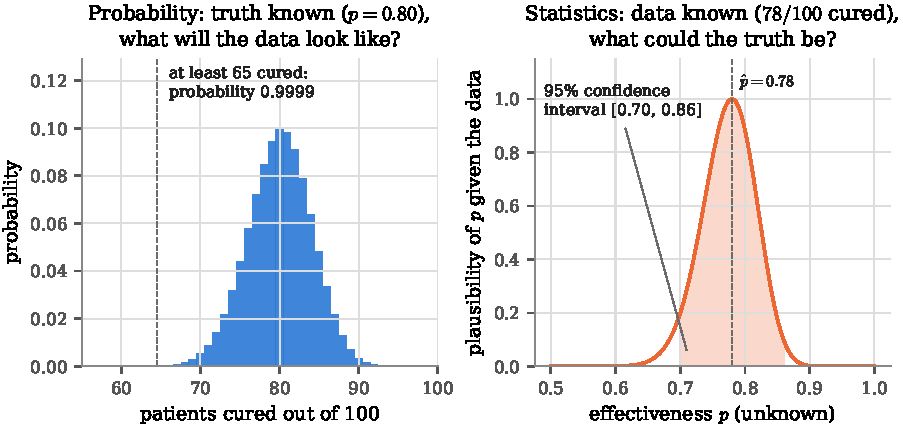
\includegraphics[width=\textwidth]{fig_probability_vs_statistics}
\caption{The drug example in both directions. Left, probability: the effectiveness $p = 0.80$ is known, so the number cured out of $100$ has a known distribution (Binomial), and the probability of at least $65$ cures is a computable $0.9999$. Right, statistics: $78$ of $100$ were cured and $p$ is unknown; the curve shows how plausible each value of $p$ makes the data (it is the likelihood of \cref{ch:likelihood}, scaled to peak at $1$), and the shaded band is the $95\%$ confidence interval $[0.70, 0.86]$ of \cref{ch:confidence-intervals}.}
\label{fig:probstat}
\end{figure}

Notice what the right-hand panel is \textit{not}.
It isn't a probability distribution for $p$: in this book $p$ is a fixed unknown number, not a random variable, and the curve is a plausibility ranking of candidate truths, not a density.
The one place where $p$ does get a distribution is \cref{ch:bayes-intro}, and the difference is the whole point of that chapter.

\begin{bridge}[descriptive and inferential statistics]
An introductory course divides statistics into descriptive (summarize the data you have) and inferential (say something about the population you don't have).
This book is entirely about the second, and it adds the step the introductory course leaves implicit: a mathematical model of how the data were produced, precise enough that the inferential statements can be proved rather than asserted.
The model is the thing on the left of the diagram, and every method in the book is a way of traveling the orange arrow with a guarantee attached.
\end{bridge}

\section{The kiss experiment}
\label{sec:kiss-test}

Newborn babies, lying on their backs, turn their heads to the right more often than to the left.
A 2003 paper in \textit{Nature} asked whether that preference survives into adulthood, and looked for it in an unexpected place: which way couples turn their heads when they kiss.\footnote{O.~G\"unt\"urk\"un, `Adult persistence of head-turning asymmetry', \textit{Nature} 421 (2003), 711.}
The author watched kissing couples in public places (airports, train stations, beaches and parks) in the United States, Germany and Turkey, and recorded for each couple which way their heads turned.

Let $p$ denote the proportion of couples who turn their heads to the right when kissing.
The statistical experiment: observe $n$ kissing couples and record each outcome, $1$ for right and $0$ for left.
Estimate $p$ with the proportion $\hat{p}$ of couples who turned right.
Of the $n = 124$ couples observed, $80$ turned to the right, so
\[
\hat{p} = \frac{80}{124} = 64.5\%.
\]

Two things about the number $124$ because the whole book turns on them.
It is small, and it is small for a reason: each observation needs an observer in a public place at the right moment, close enough to see which way the heads turn, and a kiss is over in seconds.
And it is the only sample there is: the study is published, and the question is what these $124$ observations can be made to say.
Everything that follows is about how much a sample of this size can be made to say.

Now some random intuition.
$64.5\%$ is much larger than $50\%$, so there seems to be a preference for turning right.
But suppose the data had been right, right, left, that is $n = 3$: that's $66.7\%$ to the right, an even bigger number.
Better evidence?
Obviously not; intuitively you need a large enough sample size to make a call.
How large?
Another way to put the problem: for $n = 124$, what is the minimum number of couples turning right that you would need to see to be convinced that $p > 50\%$?
$63$? $72$? $75$? $80$?
Mathematical modeling is needed to understand the accuracy of this procedure, and the number turns out to be $72$ (\cref{sec:kiss-trinity}).

\section{Modeling assumptions}
\label{sec:kiss-assumptions}

Formally, the procedure consists of the following.
For $i = 1, \ldots, n$, define $R_i = 1$ if the $i$-th couple turns to the right and $R_i = 0$ otherwise.
The estimator of $p$ is the sample average
\[
\hat{p} = \bar{R}_n = \frac{1}{n} \sum_{i=1}^n R_i.
\]

What is the accuracy of this estimator?
To answer, you propose a statistical model that describes, or approximates well, the experiment.
You think of the $R_i$'s as random variables so that $\hat{p}$ is also a random variable, and then you study its fluctuations.

Coming up with a model consists of making assumptions on the observations $R_i$, $i = 1, \ldots, n$, in order to draw statistical conclusions.
Here are the three assumptions this model makes:
\begin{enumerate}[nosep]
\item Each $R_i$ is a random variable.
\item Each of the r.v.s $R_i$ is Bernoulli with parameter $p$.
\item $R_1, \ldots, R_n$ are mutually independent.
\end{enumerate}

Let's discuss these assumptions, since each one is a decision rather than a fact.
\begin{enumerate}[nosep]
\item Randomness is a way of modeling lack of information.
With perfect information about the conditions of the kiss (the couple's heights, which side each was standing on, which way each habitually turns, what is going on in their minds), physics and psychology might let you predict the outcome.
You don't have that information, so you treat the outcome as random.
\item Given (1), the $R_i$'s are necessarily Bernoulli r.v.s since $R_i \in \{0, 1\}$; the only question is their parameters.
They could have a different parameter for each couple, $R_i \sim \Bern(p_i)$, but you don't have enough information in the data to estimate $124$ separate $p_i$'s from $124$ observations.
So you simply assume the observations come from the same process: $p_i = p$ for all $i$.
\item Independence is reasonable because the couples were observed in many different places, in three countries, at different times.
It would fail if, say, several of the $124$ observations were the same couple seen more than once, or if couples watched each other and copied.
\end{enumerate}

A collection of r.v.s $X_1, \ldots, X_n$ satisfying (2) and (3), each with the same distribution and all mutually independent, is called \textbf{independent and identically distributed}, abbreviated i.i.d., and the book writes $X_1, \ldots, X_n \iid \Bern(p)$.
Nearly every model in this book starts from an i.i.d.\ sample.

\begin{intuition}[complicated process $=$ simple process $+$ random noise]
That equation is the one-line philosophy of statistical modeling.
Some processes are random in fact (a biased coin, measurement error, which customer walks in next).
Others are deterministic but far too complex to describe (which way a particular couple turns).
Statistical modeling treats the second kind like the first: pick a plausible simple process (every couple turns right with the same probability $p$) and a noise distribution (Bernoulli), and let the noise absorb everything you chose not to model.
Good modeling consists in choosing a simple process and a noise distribution that are plausible for the data at hand, and the trade is always the same: more assumptions buy fewer parameters to estimate, at the price of being wrong if the assumptions are.
\Cref{ch:models} makes this precise with the definition of a statistical model.
\end{intuition}

\section{Population versus sample}
\label{sec:kiss-population}

In the model, what is $\hat{p} = \bar{R}_n$ a sample \textit{from}?
Here is a thought experiment that answers it.
Assume there is a total population of $5{,}000$ couples who kiss in airports, and assume for the sake of argument that $p = 35\%$, or that $p = 65\%$.
What do samples of size $124$ look like in each case?
\Cref{fig:kisssamples} answers by drawing the exact distribution of $\bar{R}_n$ under the i.i.d.\ model for each assumed $p$, together with the distribution for samples of size $3$.
(For a population of $5{,}000$ the draws are without replacement, which changes the standard deviation of the picture by about one percent; the bridge box below says why the book works with the i.i.d.\ model instead.)

\begin{figure}[htbp]
\centering
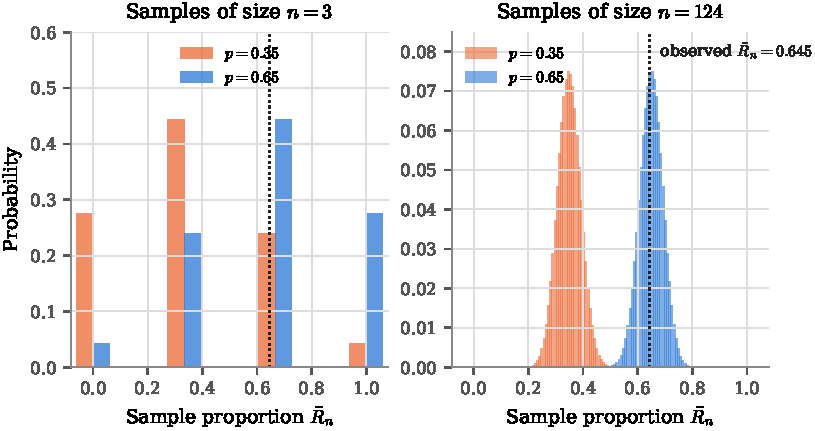
\includegraphics[width=\textwidth]{fig_kiss_samples}
\caption{What samples look like under two hypothetical truths. The bars are the exact (Binomial) distribution of the sample proportion $\bar{R}_n$ when the true proportion is $p = 0.35$ (orange) and when it is $p = 0.65$ (blue). With $n = 3$ (left) the two distributions overlap heavily: two or more right turns out of $3$ has probability $0.28$ under $p = 0.35$ and $0.72$ under $p = 0.65$, so three couples settle nothing. With $n = 124$ (right) the distributions have separated, and the observed $0.645$ (dotted line) is typical under $p = 0.65$ and essentially impossible under $p = 0.35$ (probability about $2 \times 10^{-11}$ of a proportion that large).}
\label{fig:kisssamples}
\end{figure}

The figure is the whole subject in miniature.
Under each candidate truth, probability tells you what the data would look like.
Statistics runs that backwards: the observed data are typical under some candidate truths and absurd under others, and the first group is your answer.
The rest of the book is about doing this with guarantees, and about doing it when the candidate truths form a continuum rather than two values.

\begin{bridge}[population, sample, parameter, statistic]
An introductory course describes a population (all kissing couples), a parameter of it ($p$, the proportion who turn right), a sample ($124$ couples) and a statistic computed from the sample ($\hat{p} = 0.645$) that estimates the parameter.
This book keeps all four words and changes what sits behind the first one.
The population is no longer a finite list of $5{,}000$ couples; it is a probability distribution, $\Bern(p)$, and a sample is $n$ independent draws from it.
The change is what makes the mathematics go: a finite population would make the draws slightly dependent (drawing without replacement) and would make the answer depend on the population size, while the distribution model gives clean results that hold whatever the size of the population and whether or not you can even list it.
\end{bridge}

Why does the model need probability?
Because you need to understand probabilistic aspects of the distribution of the random variable
\[
\hat{p} = \bar{R}_n = \frac{1}{n} \sum_{i=1}^n R_i.
\]
Specifically, you need to be able to answer questions such as:
\begin{itemize}[nosep]
\item Is the expected value of $\hat{p}$ close to the unknown $p$?
\item Does $\hat{p}$ take values close to $p$ with high probability?
\item Is the variance of $\hat{p}$ large? That is, does $\hat{p}$ fluctuate a lot?
\end{itemize}
Most of the probability tools needed are about averages of independent random variables, which is why Part II is about exactly that, once \cref{ch:models} has said what a model is.
For the kiss experiment the three answers are: $\E[\hat{p}] = p$ exactly; $\hat{p}$ is close to $p$ with high probability once $n$ is large (the Law of Large Numbers, \cref{ch:lln}); and $\var(\hat{p}) = p(1-p)/n$, which at $n = 124$ (and evaluated at $p = 0.645$, since $p$ itself is unknown) makes the typical fluctuation of $\hat{p}$ about $0.043$ (the Central Limit Theorem, \cref{ch:clt}, says the fluctuations are Gaussian).

\begin{pitfall}[is $64.5\%$ an estimator?]
No: $64.5\%$ is an estimate, and an estimate is not an estimator.
An \textbf{estimator} is a rule for turning data into a guess, $\hat{p} = \bar{R}_n$, and because the data are random the estimator is a random variable; it has an expectation, a variance and a distribution, and those are what \cref{fig:kisssamples} draws.
An \textbf{estimate} is the number the rule produced on the one sample you have, $\bar{r}_n = 0.645$.
It is one draw from the estimator's distribution: before the study, $\bar{R}_n$ could have come out anywhere from $0$ to $1$ with probabilities set by $p$, and the study produced one of those values.
Once observed it is a fixed number; the distribution belongs to the rule that produced it, not to the number.
Every statement about accuracy in this book is a statement about the estimator; the estimate is what you report.
\Cref{ch:lln} returns to this distinction under the name `theoretical sample mean', and \cref{sec:models-sample-space} walks the whole chain from the sample space to the number.
Outside that discussion and this box, the book follows the usual practice and writes the upper-case symbol with its realized value, $\bar{R}_n = 0.645$, trusting the context to say which of the two is meant.
\end{pitfall}

\section{The trinity of statistical inference}
\label{sec:kiss-trinity}

Everything statistical inference does falls under three headings, together called the trinity of statistical inference.
Here is each one as a sentence about the kiss experiment, with the chapter that makes the sentence precise.

\begin{enumerate}
\item \textbf{Estimation.} `$\hat{p} = \bar{R}_n$ is an estimator for the proportion $p$ of couples who turn their heads to the right.'
What makes it a good one? It is unbiased, its variance shrinks like $1/n$, and it is consistent.
\Cref{ch:estimators} defines these properties and compares estimators by them; \cref{ch:likelihood} shows that $\bar{R}_n$ is also the maximum likelihood estimator.

\item \textbf{Confidence intervals.} `$[0.56, 0.73]$ is a $95\%$ confidence interval for $p$.'
A range of truths under which the observed data are not surprising, with a guarantee about how often the procedure captures the truth.
\Cref{ch:confidence-intervals} builds this interval three ways and explains what the $95\%$ does and does not mean.

\item \textbf{Hypothesis testing.} `We find statistical evidence that more couples turn their heads to the right when kissing.'
A yes/no decision about $p$ with a controlled chance of being wrong.
\Cref{ch:tests-foundations} sets up the decision and \cref{ch:wald-lrt} supplies the general tests.
Here is the answer to the question of \cref{sec:kiss-test}: if the truth were $p = 1/2$, that is, if couples had no preference for either side, then the number turning right among $124$ couples would reach $72$ or more with probability $0.044$ and $75$ or more with probability $0.012$.
So $63$ right turns would be unremarkable (probability $0.46$ of at least that many), $72$ would be mild evidence, and $80$, which has probability $0.0008$ of being reached under $p = 1/2$, is strong evidence.
So $72$ is the threshold at the conventional $5\%$ level for this one-sided question; the two-sided version of \cref{ch:tests-foundations}, which also guards against $p < 1/2$, asks for $74$.
(Both numbers come from the exact Binomial distribution of the count; \cref{ch:tests-foundations} also derives the Gaussian-approximation versions, $72$ and $73$, and says why they can differ.)
\end{enumerate}

All three are statements about the same random variable $\bar{R}_n$, built from the same three modeling assumptions, and \cref{fig:trinity} draws them on one axis.
Change an assumption, for instance drop independence, and all three change.

\begin{figure}[htbp]
\centering
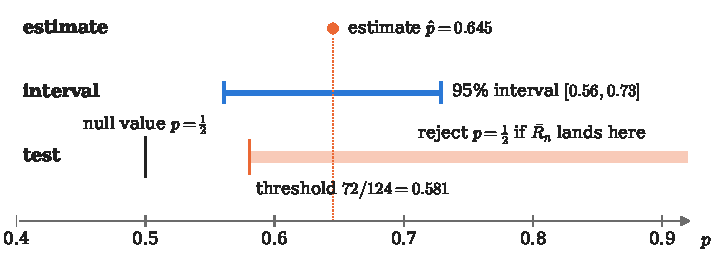
\includegraphics[width=\textwidth]{fig_trinity_axis}
\caption{The trinity on one axis. Every statement is about where $p$ sits on the line. The estimate is a point, $\hat{p} = 0.645$. The $95\%$ confidence interval is a bracket around it, $[0.56, 0.73]$: the truths under which the data are not surprising. The test compares the data to one particular truth, $p = \frac12$: if the observed proportion lands at or beyond the threshold $72/124 = 0.581$ (shaded), the data count as evidence against $p = \frac12$ and for $p > \frac12$. The threshold is set so that this happens only $5\%$ of the time when $p = \frac12$ really is the truth. \Cref{ch:confidence-intervals} and \cref{ch:tests-foundations} build the bracket and the threshold; the point is where both start.}
\label{fig:trinity}
\end{figure}

\section{What this book is and is not}
\label{sec:kiss-course}

This book has two aims: to introduce the mathematical theory behind statistical methods, and to supply theoretical guarantees for the methods you already use.
By the end you should be able to take a real-life situation like the kiss experiment, state it as a statistical problem in mathematical terms, choose methods appropriate to it, and say what those methods do and do not license you to conclude.
Four things recur throughout: the derivation of a standard method rather than its recipe, the justification of a quantitative statement from a stated set of modeling assumptions, the mathematics that arises in statistics and is worth seeing in its own right, and a toolbox of arguments that transfers to models the book never mentions.

Three things are outside its scope.
Applied modeling, meaning which data to collect and how to clean what you collected, is a separate subject, and the kiss experiment illustrates the point: \cref{sec:kiss-assumptions} takes the $124$ observations as given and says nothing about where and when to watch, or how to decide which way a pair of heads turned.
Implementation is not treated at all, and no formula here is tied to a particular piece of software.
And the aim is not a list of named methods: the general machinery of \cref{ch:wald-lrt} delivers whole families of tests at once, including most of the named ones, which is the reason for building it.
Where the undergraduate version of an idea makes the general version easier to see, that version appears in a box labeled `From undergraduate statistics'.

\section{What comes next}
\label{sec:kiss-next}

The three questions of \cref{sec:kiss-population} are all about the random variable $\hat{p} = \bar{R}_n$: its expectation, where it concentrates, how much it fluctuates.
The first has a one-line answer, $\E[\hat{p}] = p$.
Before any of them is answered, \cref{ch:models} turns the three assumptions of \cref{sec:kiss-assumptions} into an object, the statistical model, so that everything later can be stated for any model and not only this one.
The other two questions are about what happens as $n$ grows, and `as $n$ grows' is a limit, so Part II is about limits of random variables: \cref{ch:lln} says where $\bar{R}_n$ ends up, \cref{ch:clt} says what its fluctuations look like on the way, and \cref{ch:limit-tools} says what you may do to those limits (transform them, plug estimates into them) and still know where you are.
\Cref{ch:gaussian} then collects what you need about the Gaussian distribution, which is where all of the limits land.
If you are comfortable with limits of random variables already, \cref{ch:lln} opens with a box that says which parts of Part II are the minimal path.

\section{Summary}
\label{sec:kiss-summary}

\begin{itemize}[nosep]
\item Probability goes from a known mechanism to the data it produces; statistics goes from observed data back to the mechanisms that could have produced them. Same diagram, opposite arrows.
\item The kiss experiment: $n = 124$ couples, $80$ turned right, $\hat{p} = \bar{R}_n = 0.645$. It is the running example of the book.
\item Three modeling assumptions turn the data into mathematics: each $R_i$ is random, each is $\Bern(p)$ with the same $p$, and they are independent. Together: $R_1, \ldots, R_n \iid \Bern(p)$. Each assumption is a choice with a justification.
\item The population is a probability distribution, not a list; a sample is $n$ independent draws. The estimator $\hat{p}$ is a random variable; the estimate $0.645$ is one realization of it.
\item The trinity of inference: estimation (is $\hat{p}$ a good guess?), confidence intervals (which truths are compatible with the data?), hypothesis testing (is $p > 1/2$?). Every inferential method in this book is one of the three.
\end{itemize}

\section{Exercises}
\label{sec:kiss-exercises}

\begin{exercise}
Two dice are rolled and you win \$100 if you called the sum. Which total should you call, and what is your expected winning? Why is this a probability question rather than a statistics question?
\end{exercise}
\begin{solution}
Call $7$: six of the $36$ equally likely pairs sum to $7$, more than any other total, so the probability is $1/6$ and the expected winning is $100/6 \approx \$16.67$. The mechanism (fair, independent dice) is known in full, so there is nothing to learn from data; the answer is deduced.
\end{solution}

\begin{exercise}
In the drug example, verify the probability statement: if the drug cures each patient independently with probability $0.8$, show that the number cured out of $100$ has mean $80$ and standard deviation $4$, and explain why `at least $65$ cured' has probability very close to $1$.
\end{exercise}
\begin{solution}
The count is $\text{Bin}(100, 0.8)$ with mean $np = 80$ and standard deviation $\sqrt{np(1-p)} = \sqrt{16} = 4$. The value $65$ is $15/4 = 3.75$ standard deviations below the mean; a Gaussian approximation gives $\Pr(\text{at least } 65) \approx \Phi(3.75) \approx 0.9999$, and the exact Binomial computation gives $0.99985$.
\end{solution}

\begin{exercise}
Suppose the kiss data had been $n = 3$ couples, two turning right. Under the hypothetical truths $p = 0.35$ and $p = 0.65$, compute the probability of observing at least two right turns. What does the comparison tell you?
\end{exercise}
\begin{solution}
$\Pr(\text{at least } 2) = 3p^2(1-p) + p^3$, which is $0.282$ at $p = 0.35$ and $0.718$ at $p = 0.65$. The data are only about $2.5$ times more probable under the larger $p$, so three couples cannot distinguish the two truths; with $124$ couples the corresponding ratio is astronomically large (\cref{fig:kisssamples}).
\end{solution}

\begin{exercise}
Which of the three modeling assumptions would be violated in each case, and in which direction would it push $\hat{p}$? (a) The observer recorded each couple twice by mistake. (b) Half the couples were observed at a single wedding reception where the photographer told everyone to turn right. (c) The observer only recorded couples whose faces were visible from where the observer stood.
\end{exercise}
\begin{solution}
(a) Independence: the $124$ records are really $62$ independent observations, so $\hat{p}$ is as variable as a sample of $62$, not $124$, though its expectation is still $p$. (b) Identical distribution and independence: those couples share a $p_i$ near $1$ that is not the population's $p$, and they all followed the same instruction, so their outcomes are not independent; $\hat{p}$ is pushed upward. (c) The sample is not drawn from the population of interest at all: if being visible is related to the direction of the turn (it plausibly is, since from one side the observer sees the faces of couples who turn one way and the backs of the heads of couples who turn the other), the $R_i$ are Bernoulli with a parameter that differs from $p$, and no amount of data fixes it. The third is the most dangerous because it is invisible in the data.
\end{solution}

\chapter{Statistical Models and Identifiability}
\label{ch:models}

\begin{chaptergoals}
\begin{itemize}[nosep]
\item What a statistical model is: a sample space and a family of candidate distributions indexed by a parameter. The whole of the rest of the book happens inside this object.
\item The chain from the abstract sample space to the numbers in the data file, walked once for the kiss experiment: outcomes, random variables as functions on them, and observations as those functions evaluated at the outcome that happened.
\item The trade that modeling always makes: assumptions buy fewer parameters to learn, at the price of being wrong if the assumptions are. The siblings example, drawn both ways.
\item Well-specified models, and parametric versus nonparametric ones.
\item Identifiability: when the distribution of the data pins down the parameter, and when it doesn't, with the standard example drawn in the parameter space so you can see what fails.
\item Gaussian mixture models, as a generative story and as an example of a model whose parameter is identifiable only up to relabeling.
\end{itemize}
\Cref{ch:kiss} made three assumptions about the kiss experiment and called the result a model. This chapter says what a model is in general, so that everything from Part III on can be stated for any model and not only the Bernoulli one.
\end{chaptergoals}

\section{The rationale behind statistical modeling}
\label{sec:models-rationale}

\Cref{ch:kiss} was about one estimator, $\hat{p} = \bar{R}_n$, under one set of assumptions.
To say what estimators, intervals and tests are in general, you first have to fix the object they all live in: a model, which is the three assumptions of \cref{sec:kiss-assumptions} written as a mathematical object.
The rationale behind statistical modeling can be outlined as follows:
\begin{itemize}
\item Let $\Xton$ be $n$ independent copies of $X$.
The goal of statistics is to learn the distribution of $X$.

\textbf{NB:} It's crucial to understand this notation, this way of specifying problems, and, most importantly, the relationship between the $n$ i.i.d.\ r.v.s $\Xton$ and the r.v.\ $X$.
Each of the $n$ i.i.d.\ r.v.s $\Xton$ has the same distribution as the r.v.\ $X$.
The relationship between $X$ and $\Xton$ can be understood as follows:
\begin{enumerate}[nosep]
\item $X$ is the underlying r.v.\ of interest, with an unknown distribution that you want to learn.
\item $\Xton$ are $n$ r.v.s that form your sample of observations drawn from the same distribution as $X$.
This is all-important: When you see something like `Suppose $\Xton$ are $n$ independent copies of $X$' you should \textit{automatically interpret these $n$ variables as your sample data}.
\end{enumerate}
By observing the values of $\Xton$, you can make inferences about the distribution of $X$.

\item If $X \in \{0,1\}$, then it's Bernoulli and you only have to learn the parameter $p$.
That was the kiss experiment.

\item It can be more complicated.
Take a (partial) dataset of the number of siblings, including self, collected from college students:
\[
2, 3, 2, 4, 1, 3, 1, 1, 1, 1, 1, 2, 2, 3, 2, 2, 2, 3, 2, 1, 3, 1, 2, 3, \ldots
\]
If $X \in \{1, 2, 3, 4, 5, 6, \geq 7\}$, each with a different probability $\Pr(X = x)$, then you could make no assumption and try to learn the whole PMF: that's $7$ parameters to learn (six, really, since they sum to one).

\item Or you could assume that $X - 1 \sim \Pois(\lambda)$.
That's only 1 parameter, $\lambda$, to learn.
\Cref{fig:siblings} shows both on the siblings data.
The empirical PMF is seven numbers, six of them free since they sum to one; the model is one number, $\hat\lambda$, set to the sample mean minus one.
The model fits well here; where such a model didn't fit, the fault would be the assumption's, not the data's.

\item \textbf{NB:} It's important to keep in mind that parameters define distributions.
What is meant is that, suppose you're considering the family of Gaussian distributions.
Once you specify $\mu$ and $\sigma^2$, you've fixed the distribution.
Learning the parameter and learning the distribution are the same task.
(The Gaussian family appears in several examples of this chapter, written $\Gauss(\mu, \sigma^2)$ with the variance second, and with $\Phi$ for the CDF of $\Gauss(0,1)$; \cref{ch:gaussian} is its full treatment, and the notation page has what is needed here.)
\end{itemize}

\begin{figure}[htbp]
\centering
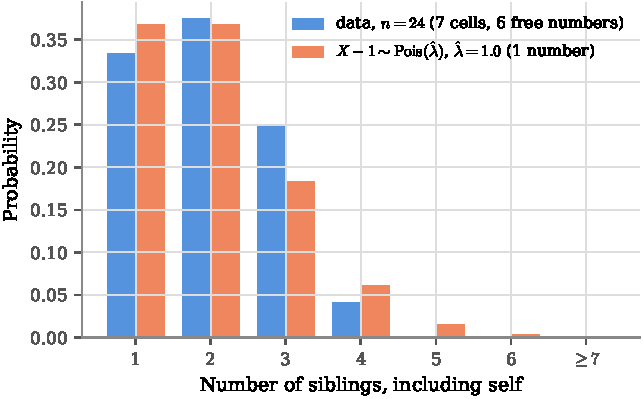
\includegraphics[width=0.78\textwidth]{fig_siblings_model}
\caption{The siblings data ($n = 24$ values) as an empirical PMF (blue), next to the fitted one-parameter model $X - 1 \sim \Pois(\hat\lambda)$ (orange), with $\hat\lambda$ the sample mean minus one.}
\label{fig:siblings}
\end{figure}

\begin{intuition}[assumptions are currency]
Every assumption you add to a model buys you something and costs you something.
`$X - 1$ is Poisson' reduces seven unknowns to one, which means $24$ observations go a long way instead of being spread over seven cells, and it lets you say things about families of $8$ siblings that you never observed.
What it costs is the possibility of being wrong: if the real PMF isn't Poisson-shaped, no amount of data will make the model right, and the estimate of $\lambda$ will be a precise estimate of the wrong thing.
The phrase for this is that a model should be plausible, and the mathematics that follows assumes it is.
Checking the assumption is the job of the goodness-of-fit tests in \cref{ch:gof}.
\end{intuition}

\section{Statistical models}
\label{sec:models-definition}

\begin{definition}[Statistical model]
\label{def:statmodel}
Let the observed outcome of a statistical experiment be a sample $\Xton$ of $n$ i.i.d.\ r.v.s in some sample space $E$ (usually $E \subseteq \real$; the requirement that $E$ be measurable is a technicality, see \toolkit{sec:math-rv}) and denote by $\Pr$ their common distribution.
A \textbf{statistical model} associated to that statistical experiment is a pair:
\[
\left(E, (\Pr_\theta)_{\theta \in \Theta} \right),
\]
where:
\begin{itemize}[nosep]
\item $E$ is the \textbf{sample space} for $X$; that is, the set containing all possible outcomes of $X$.
The sample space is therefore also where your observations, $\Xton$, live.
\item $(\Pr_{\theta})_{\theta \in \Theta}$ is a family of probability distributions on $E$, the candidate distributions for $X$.
\item $\Theta$ is the \textbf{parameter space}; that is, a set consisting of the possible values of $\theta$.
\end{itemize}
\end{definition}

\begin{inwords}
\textbf{In words.} A model is a list of candidate explanations for the data: where an observation can land ($E$), and every distribution you are willing to consider as the one that produced it, with a label $\theta$ on each.
\par\smallskip
\textbf{For the kiss data.} $E = \{0, 1\}$, the candidates are the $\Bern(p)$ distributions, one for each $p \in (0,1)$, and the label is $p$ itself. `Learn the model' means `find out which label is right'.
\end{inwords}

\textbf{Note:} A \textbf{probability measure} or \textbf{probability distribution} takes an event $A \subseteq E$ as input and returns $\Pr_\theta(A)$ \toolkit{sec:math-rv}.
It is assumed to satisfy the usual axioms of probability.
Most importantly, a probability measure is not a PMF or PDF.
A probability measure assigns probabilities to events in the sample space, while a PMF or PDF assigns probabilities (or densities) to specific values of a discrete or continuous r.v.
The two determine each other, so in practice you write down the family by writing down its PMFs or PDFs, as in the examples below, but the object in the definition is the distribution.

\Cref{fig:modelfamilies} is the picture to keep in mind: a model is a family of distributions, and the parameter is the label that picks one out.
In the top row, two one-parameter families; sliding the parameter moves you through the family.
In the bottom row, the Gaussian family has a two-dimensional parameter space, drawn on the left, and each point of it is one distribution, drawn on the right.
The arrow $\theta \mapsto \Pr_\theta$ from the left of the figure to the right is what the definition is about, and \cref{sec:models-identifiability} asks whether it ever sends two points to the same distribution.

\begin{figure}[htbp]
\centering
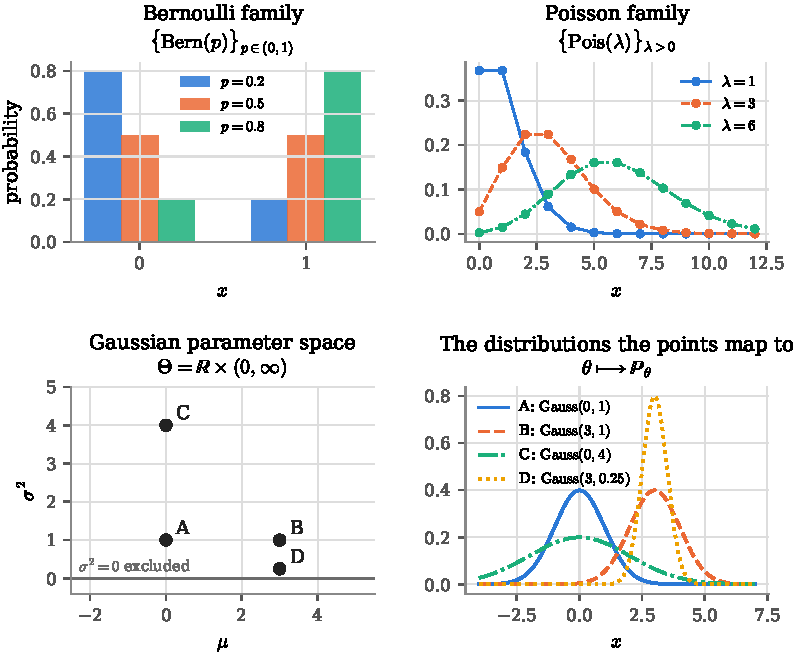
\includegraphics[width=\textwidth]{fig_model_families}
\caption{Top: the Bernoulli family at three values of $p$, and the Poisson family at three values of $\lambda$. Bottom: four points A to D in the Gaussian parameter space $(\mu, \sigma^2)$, left, and the densities they map to, right.}
\label{fig:modelfamilies}
\end{figure}

\subsection{Examples of parametric models}

For parametric models (defined in \cref{sec:models-parametric}: the parameter is a list of finitely many numbers), the parameters live in some space that's a subset of $\real^d$ and the parameters can be represented by a vector.
Here are some canonical examples of parametric models:
\begin{enumerate}
\item For $n$ Bernoulli trials: $\left( \{0, 1\}, (\Bern(p))_{p \in (0,1)} \right)$.
The vectors of parameters thus consist of singletons $(p)$.

\item If $\Xton \iid \Pois(\lambda)$ for some unknown $\lambda > 0$: $\left( \mathbb{N}, (\Pois(\lambda))_{\lambda > 0} \right)$.
The vectors of parameters thus consist of singletons $(\lambda)$.

\item If $\Xton \iid \Gauss(\mu, \sigma^2)$ for some unknown $\mu \in \real$ and $\sigma^2 > 0$:
\[
\left( \real, (\Gauss(\mu, \sigma^2))_{(\mu, \sigma^2) \in \real \times (0, \infty)} \right).
\]
The vector of parameters has length 2 and is given by $(\mu, \sigma^2)$.

\item If $\Xton \iid \Gauss_d(\mu, \ident_d)$ for some unknown $\mu \in \real^d$: $\left( \real^d, (\Gauss_d(\mu, \ident_d))_{\mu \in \real^d} \right)$.
The vector of parameters is $\mu$ itself, of length $d$.

\item If $\Xton \iid \text{Unif}([0, a])$ for some unknown $a > 0$: $\left( \real_+, (\text{Unif}([0, a]))_{a > 0} \right)$.
Not $\left( [0, a], \ldots \right)$: see the pitfall below.
\end{enumerate}

Sometimes there's no simple notation like $\Bern(p)$ for the family and you have to be more explicit.
The linear regression model: $(X_1, Y_1), \ldots, (X_n, Y_n) \in \real^d \times \real$ are i.i.d.\ with $Y_i = \beta^\top X_i + \epsilon_i$, $\epsilon_i \iid \Gauss(0,1)$ independent of $X_i \sim \Gauss_d(0, \ident_d)$, for an unknown $\beta \in \real^d$.
Here $E = \real^d \times \real$, $\Theta = \real^d$, and $\Pr_\beta$ is the joint distribution of the pair $(X, Y)$ that this recipe produces.
\Cref{ch:regression-multi} is about this model in a slightly different form: the $X_i$ treated as fixed numbers rather than Gaussian draws, and the error variance $\sigma^2$ unknown, which makes $\Theta = \real^d \times (0, \infty)$ and makes the $Y_i$ independent but no longer identically distributed, since each has its own mean $\beta^\top x_i$.
Treating the predictors as fixed is what lets the regression chapter condition on them and still have a model in the sense of \cref{def:statmodel}.

\begin{pitfall}[the sample space must not depend on the parameter]
Which of these is a statistical model for $n$ Bernoulli trials: $\left( \{1\}, (\Bern(p))_{p \in (0,1)} \right)$ or $\left( \{0,1\}, (\Bern(p))_{p \in (0.2, 0.4)} \right)$?
Only the second.
The first has a sample space that leaves out an outcome the distributions put mass on; a Bernoulli r.v.\ takes the value $0$, so $\{1\}$ isn't where the observations live.
The second is a model, just one that assumes $p$ is between $0.2$ and $0.4$ (which may or may not be well-specified, the next section's question).
Similarly, for $\Xton \iid \text{Unif}([0, a])$ with $a$ unknown, the model is $\left( \real_+, (\text{Unif}([0, a]))_{a > 0} \right)$ and not $\left( [0, a], \ldots \right)$: the sample space is fixed before you know $a$, so it has to be a set that contains every observation for every candidate $a$.
Any such set will do ($\real$ works too); the convention in this book is the smallest natural one.
A sample space that mentions the unknown parameter is not a sample space.
\end{pitfall}

\begin{bridge}[the model was always there]
In an introductory course the model is a sentence: `assume the data are normally distributed', `assume each trial succeeds with the same probability'.
This book makes the sentence into an object with three parts, and the point of doing so is that every later statement can name exactly what it depends on.
`The sample mean is unbiased' is a statement about $\E_\theta[\bar{X}_n]$ for every $\theta \in \Theta$; `the $t$-test has level $5\%$' is a statement that holds for every member of the Gaussian family; `the estimator is consistent' means $\hat{\theta}_n \to \theta$ under $\Pr_\theta$ for every $\theta$.
When a method fails in practice, it is often because the data came from outside the family, and you can only say that if the family is written down.
\end{bridge}

\section{From the sample space to the data and back}
\label{sec:models-sample-space}

The definition says the observations live in a sample space $E$, and a random variable is, by definition, a function on a sample space $S$ \toolkit{sec:math-rv}; \cref{ch:lln} returns to that definition when it needs sequences of random variables.
These are two uses of the same phrase for two different sets, and the gap between them is where the single most common confusion in this subject lives: what is the relationship between the abstract space on which probability is defined and the concrete numbers in the data file?
This section walks the chain once, slowly, for the kiss experiment, with \cref{fig:layers} as the map.
On the left of the figure is the sample space $\Omega$, one point per complete possible outcome of the study, with the one that happened marked.
In the middle, the data are a function on $\Omega$, one row of $0$s and $1$s per outcome, and the marked row is the data set you have.
On the right, the statistic $\bar R_n$ is another function on $\Omega$; over all outcomes weighted by their probabilities it has a distribution, the bars, and the marked outcome gives the one value you observe, $\bar r_n = 8/12$.
Nothing travels from right to left: the dashed arrow is inference, which holds the one value up against the distribution of the rule.

\begin{figure}[htbp]
\centering
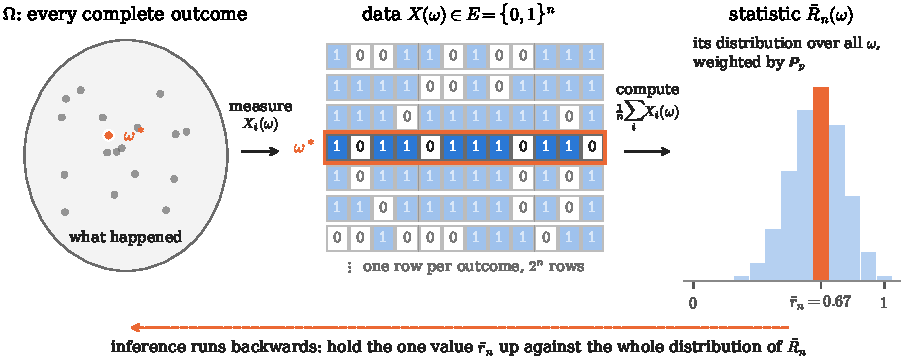
\includegraphics[width=\textwidth]{fig_sample_space_layers}
\caption{The sample space $\Omega$ (left), the data as one row of $0$s and $1$s per outcome (middle), and the statistic $\bar R_n$ with its distribution (right), for a kiss experiment with $n = 12$. The outcome that happened is marked in orange.}
\label{fig:layers}
\end{figure}

\textbf{Layer one: the sample space.}
An outcome $\omega$ of the study is everything that could happen, in full detail: which $124$ couples were observed, where and in which order, and which way each one turned.
The set of all such outcomes is the sample space, written $\Omega$ here ($S$ in the toolkit and in \cref{ch:lln}).
It is as abstract as the subject gets, and you never see an element of it.
What you see is what your measuring instruments report about the one $\omega$ that occurred.

\textbf{Layer two: random variables are the measuring instruments.}
A random variable is a function on $\Omega$ \toolkit{sec:math-rv}.
The instrument for couple $i$ is $R_i$, with $R_i(\omega) = 1$ if, in outcome $\omega$, couple $i$ turned right and $0$ otherwise.
The data vector $(R_1, \ldots, R_n)$ is a function on $\Omega$ too, with values in $E^n = \{0,1\}^n$; one row of \cref{fig:layers} per outcome.
And $\bar{R}_n = \frac{1}{n}\sum_i R_i$ is yet another function on $\Omega$.
That is all `the estimator is a random variable' means: a rule that could be applied to any outcome, written down before you know which outcome you will get.

\textbf{Layer three: the observations are those functions evaluated at the outcome that happened.}
Nature picked one $\omega^*$.
Your data are $r_1 = R_1(\omega^*), \ldots, r_n = R_n(\omega^*)$, and your estimate is $\bar{r}_n = \bar{R}_n(\omega^*) = 0.645$.
Going from the sample space to the observations is `plug in the $\omega$ that occurred'.
A realization is one evaluation of a function; a distribution is how often each value would come up across all of $\Omega$, weighted by probability.
The realized number $0.645$ is one draw from the distribution of $\bar{R}_n$; after it is observed it is a fixed number, and the distribution belongs to the rule, not to the number (the pitfall in \cref{sec:kiss-test}).

\textbf{Going back is not an inverse.}
You never recover $\omega^*$ from the data, and you do not need to.
What inference does instead is ask, for each candidate $\theta$: across all the outcomes that could have occurred under $\Pr_\theta$, how often would $\bar{R}_n$ have landed near the value it took?
The one number is held up against the whole distribution of the rule, and the candidates under which it would have been typical are the plausible ones.
That is the dashed arrow in \cref{fig:layers}, and it is what every confidence interval and test in this book does.

\begin{intuition}[the trick that makes $\Omega$ concrete]
Since $\Omega$ only ever enters through the random variables defined on it, you may as well take $\Omega$ to be the set of data sets you could have gotten.
For the kiss experiment that is $\Omega = \{0,1\}^{124}$, a finite set with $2^{124}$ elements, and under the model $\Pr_p(\omega) = p^{\#\text{ones}}(1-p)^{\#\text{zeros}}$.
Every row of \cref{fig:layers} is a point of this $\Omega$, and $R_i(\omega)$ is just `the $i$-th entry of the row'.
This is why \cref{def:statmodel} mentions $E$ and never $\Omega$: for a fixed $n$ the observable sample space $E^n$ \textit{is} the sample space, and a model is a family of probabilities on it.
The abstract $\Omega$ of probability theory is needed only when one space has to carry infinitely many random variables at once, $R_1, R_2, R_3, \ldots$ without end, which is exactly what the limit theorems of Part II need in order to say `as $n \to \infty$'.
For any fixed $n$, think $\Omega = E^n$ and nothing is lost.
\end{intuition}

\begin{bridge}[the sampling distribution, defined rather than simulated]
An introductory course introduces the sampling distribution of the sample mean by rerunning the study: draw many samples, compute $\bar{x}$ for each, draw the histogram.
That histogram is the right of \cref{fig:layers}, approximated by simulation; this chapter defines it instead, without rerunning anything, by putting a probability on $\Omega$ and asking how $\bar{R}_n(\omega)$ is distributed under it.
The two pictures agree: each simulated sample is one $\omega$, an introductory course's `many samples' are many points of $\Omega$, and the limit of the histogram as the number of samples grows is the distribution of the random variable.
\Cref{fig:twoaverages} in \cref{ch:lln} draws the same picture as rows and columns: a row is an $\omega$, the row average is $\bar{R}_n(\omega)$, and the column of row averages is the sampling distribution.
Your data set is the one row nature handed you.
\end{bridge}

\section{Well-specified models}
\label{sec:models-wellspecified}

It is almost always assumed that a statistical model is well-specified.

\begin{definition}[Well-specified]
\label{def:wellspecified}
A model $\left(E, (\Pr_\theta)_{\theta \in \Theta }\right)$ is \textbf{well-specified} if there exists some $\theta \in \Theta$ such that $\Pr = \Pr_{\theta}$, where $\Pr$ is the true distribution that generates the observed data $\Xton$.
In other words, $\Pr \in (\Pr_{\theta})_{\theta \in \Theta}$.
If $\Pr \notin (\Pr_{\theta})_{\theta \in \Theta}$, then the model is \textbf{misspecified}.
That particular $\theta$ such that $\Pr = \Pr_{\theta}$ is the \textbf{true parameter}, often written $\theta^*$, and is unknown.
\end{definition}

\begin{inwords}
\textbf{In words.} The true distribution is on your list of candidates. If it isn't, no label is right, and `the true parameter' has no meaning.
\par\smallskip
\textbf{For the kiss data.} If couples really do turn right with a single probability $p^*$, independently, the model is well-specified and $p^* \in (0,1)$ is the true parameter. If, say, the probability differed by country, no single $\Bern(p)$ reproduces the data-generating process and the model is misspecified.
\end{inwords}

\begin{center}
\begin{tikzpicture}[font=\small]
  \begin{scope}
    \draw[rounded corners=8pt, fill=boxblue!6, draw=boxblue!60!black] (0,0) rectangle (3.6,2.2);
    \node[anchor=north west, font=\scriptsize] at (0.1,2.15) {$(\Pr_\theta)_{\theta\in\Theta}$};
    \fill[boxaqua!70!black] (2.1,1.0) circle (2.2pt) node[right=1pt, font=\scriptsize] {$\Pr = \Pr_{\theta^*}$};
    \node[below, font=\scriptsize] at (1.8,-0.05) {well-specified: the truth is in the family};
  \end{scope}
  \begin{scope}[xshift=5.2cm]
    \draw[rounded corners=8pt, fill=boxblue!6, draw=boxblue!60!black] (0,0) rectangle (3.6,2.2);
    \node[anchor=north west, font=\scriptsize] at (0.1,2.15) {$(\Pr_\theta)_{\theta\in\Theta}$};
    \fill[boxorange!80!black] (4.3,1.0) circle (2.2pt) node[right=1pt, font=\scriptsize] {$\Pr$};
    \node[below, font=\scriptsize] at (2.3,-0.05) {misspecified: no $\theta$ reproduces the truth};
  \end{scope}
\end{tikzpicture}
\end{center}

Here's an example to illustrate the meaning of well-specified models:
\begin{itemize}
\item Suppose you're modeling the outcome of a coin toss using a Bernoulli distribution with parameter $p$, where $p$ represents the probability of getting heads.
Suppose further that the \textit{true} probability of getting heads is $p^* = 0.6$.
\item Now, if your model considers all possible values of $p \in (0,1)$, then it's a well-specified model because it includes the true probability distribution, the $\Bern(0.6)$ distribution, as one of the possible distributions in the family.
\item On the other hand, if your model only considers values of $p$ between, say, 0 and 0.5, then it's not well-specified because it doesn't include the true probability distribution, $\Bern(0.6)$, in the family of distributions.
\end{itemize}

The above example addresses misspecification when the true parameter value is not contained in your model's parameter space.
But a model misspecification could also be due to applying the `wrong' distribution: for example, by modeling the toss of a coin using a Gaussian distribution, or the siblings data of \cref{fig:siblings} with a shifted Poisson when the true PMF has a second bump at $5$.

One aim of a statistical experiment is to \textit{estimate} the true parameter $\theta^*$.
Another is to check $\theta^*$'s properties when they have a specific meaning determined by the context of the study.
As an example of this second aim you may want to know if $\theta^* > 2$ or if $\theta^* \neq 1/2$, which is the question of \cref{ch:tests-foundations}.

\section{Parametric, nonparametric and semiparametric models}
\label{sec:models-parametric}

It will often be assumed that the parameter space $\Theta$ is a subset of $\real^d$ for some $d \geq 1$.
In this case, when $\Theta \subseteq \real^d$ for $d \geq 1$, the model is called \textbf{parametric}.
Hence, $\Theta$ contains vectors of parameters with length $d$; a finite-dimensional space.

On the other hand, when $\Theta$ is infinite-dimensional, the model is called \textbf{nonparametric}.
The elements of $\Theta$ are then functions (a density, a CDF) rather than vectors of numbers.

Thus, the distinction between parametric and nonparametric models is a distinction between the \textit{length} of the vectors in the parameter space $\Theta$.
It is not a distinction of the \textit{number} of vectors living in the space.
For example, there is an uncountably infinite number of vectors living in the parameter space of a Bernoulli model where $\Theta = (0,1)$, but all the vectors are singletons: any number between 0 and 1.
What makes a model nonparametric is that no finite list of numbers can specify a member of the family; you'd need the value of a function at infinitely many points.

Nonparametric models typically include assumptions on the functions that describe the r.v.
For a continuous r.v.\ there are two: the PDF and the CDF.
Here are two examples of nonparametric models:
\begin{enumerate}
\item If $\Xton \in \real$ are i.i.d.\ r.v.s with unknown unimodal\footnote{A unimodal PDF increases on $(-\infty, a)$ and decreases on $(a, \infty)$ for some $a$.} PDF $f$:
\[
\left( \real, (\Pr_f)_{\{f: f \text{ is a unimodal PDF} \}} \right).
\]
\item If $\Xton \in [0,1]$ are i.i.d.\ r.v.s with unknown invertible CDF $F$:
\[
\left( [0,1],  (\Pr_F)_{\{F: F \text{ is an invertible CDF} \}} \right).
\]
\end{enumerate}
\Cref{fig:paramnonparam} draws the difference.
On the left, one number, $\lambda$, moves you along a single curve through the space of densities; the whole parametric family is this one-dimensional path.
On the right are four members of the first nonparametric family, all unimodal densities; no finite set of numbers indexes them, the family is the whole space of such shapes, and these are four points in it.

\begin{bridge}[nonparametric and distribution-free tests]
Some introductory courses teach nonparametric, or distribution-free, tests, such as the sign test and the Wilcoxon tests, for data that do not look normal.
The word `nonparametric' has this section's meaning: the test's guarantee holds for every member of a nonparametric model.
The sign test of whether a median equals $m_0$ assumes only that $\Xton$ are i.i.d.\ from some continuous distribution, a family indexed by a whole CDF rather than a list of numbers.
It counts the observations above $m_0$, and when $m_0$ is the median the count is $\Bin(n, \frac12)$ whatever the CDF is, so one threshold gives the same level for every continuous distribution with median $m_0$: that is what `distribution-free' means.
Keeping only the signs turns the problem into the kiss experiment's: with right turns as the plus signs, the one-sided $5\%$ threshold of $72$ out of $124$ in \cref{sec:kiss-trinity} is the sign test's threshold.
The Kolmogorov--Smirnov test of \cref{ch:ks} is distribution-free in the same sense.
\end{bridge}

\begin{figure}[htbp]
\centering
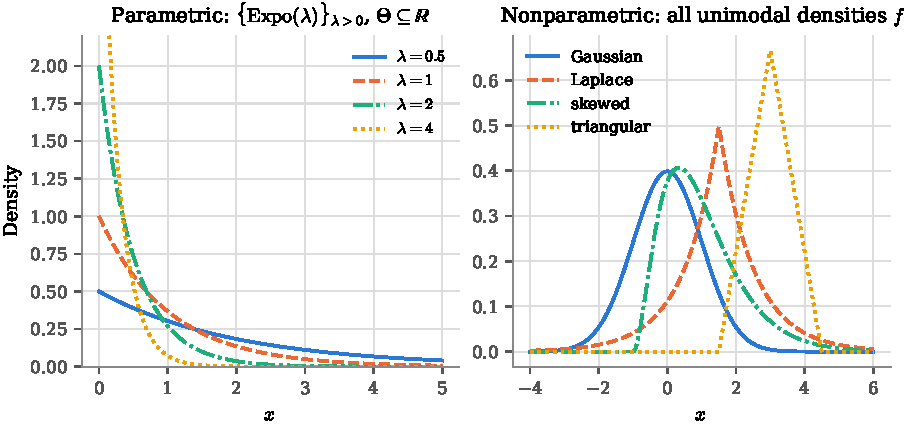
\includegraphics[width=\textwidth]{fig_parametric_vs_nonparametric}
\caption{Left: four members of the parametric family $\{\Expo(\lambda)\}_{\lambda > 0}$, at $\lambda = 0.5, 1, 2, 4$. Right: four members of the nonparametric family of all unimodal densities: Gaussian, Laplace, a skewed density and a triangular one.}
\label{fig:paramnonparam}
\end{figure}

A third kind: if $\Theta = \Theta_1 \times \Theta_2$ where $\Theta_1$ is finite-dimensional and $\Theta_2$ is infinite-dimensional, the model is \textbf{semiparametric}.
In these models you only care to estimate the finite-dimensional parameter, and the infinite-dimensional one is called a \textbf{nuisance parameter}.
The standard example is the Cox proportional hazards model from survival analysis, where the conditional CDF of a survival time $Y$ given covariates $X = x$ has the form
\[
F(t) = 1 - \exp \left( - \int_0^t h(u) e^{\beta^\top x} \, \mathrm{d}u \right),
\]
with $h$ an unknown non-negative nuisance function and $\beta \in \real^d$ the parameter of interest.
This book does not develop such models; the example is here so that you have seen what a semiparametric parameter space looks like, with $\Theta_1 = \real^d$ for $\beta$ and $\Theta_2$ the space of non-negative functions $h$.

\begin{bridge}[the regression conditions as a model]
An introductory course checks four conditions, sometimes remembered as LINE, before any inference about a regression slope: the mean of $y$ is a linear function of $x$, and the errors are independent, normal and of equal variance at every $x$.
Together they are one parametric model, with the $x_i$ treated as fixed: L is the line in $Y_i = \beta_0 + \beta_1 x_i + \epsilon_i$, and I, N and E together say $\epsilon_1, \ldots, \epsilon_n \iid \Gauss(0, \sigma^2)$, so the parameter is $(\beta_0, \beta_1, \sigma^2) \in \real^2 \times (0, \infty)$.
Replace N by `the errors are i.i.d.\ from some distribution with mean $0$ and finite variance' and the model is semiparametric: $(\beta_0, \beta_1)$ is the parameter of interest and the error distribution is an infinite-dimensional nuisance parameter.
Least squares still estimates the line without bias in that model; what N adds is the exact $t$ distribution of the slope's $t$ statistic, as it does for the $t$-test of a mean (\cref{ch:t-test}).
\end{bridge}

\section{Identifiability}
\label{sec:models-identifiability}

The first thing to ask of a model is whether it's well-specified.
You can't verify it, since the true $\Pr$ is exactly what you don't know, but you can ask whether it's plausible, and the mathematics that follows assumes it.
If it isn't, $\theta^*$ doesn't exist and `estimating the true parameter' has no meaning; what the estimators of Part IV estimate in that case is the subject of \cref{ch:distances}.
Presuming your model is well-specified, you also need to ascertain whether the parameter of the model is \textit{identifiable}.
Identifiability is a property of the parameterization: of the map from $\Theta$ to the family, not of the family itself, and not of any estimator or estimation procedure.

\begin{definition}[Identifiability]
\label{def:identifiable}
The parameter $\theta \in \Theta$ is \textbf{identifiable} if the map $\theta \mapsto \Pr_{\theta}$ is injective (one-to-one, \toolkit{sec:math-maps}).
That is:
\[
\theta_1 \neq \theta_2 \implies \Pr_{\theta_1} \neq \Pr_{\theta_2},
\]
or equivalently, taking the contrapositive:
\[
\Pr_{\theta_1} = \Pr_{\theta_2} \implies \theta_1 = \theta_2.
\]
\end{definition}

\begin{inwords}
\textbf{In words.} Different labels, different distributions. Then knowing the distribution (which is what infinitely many data would tell you) pins down the label.
\par\smallskip
\textbf{For the kiss data.} $p_1 \neq p_2$ gives $\Bern(p_1) \neq \Bern(p_2)$, since the two put different probabilities on $1$; $p$ is identifiable. The example below shows a model where two different labels give the same distribution.
\end{inwords}

\begin{center}
\begin{tikzpicture}[font=\small, >={Latex[length=2mm]}]
  \begin{scope}
    \node[font=\scriptsize] at (0.5,2.6) {$\Theta$};
    \node[font=\scriptsize] at (3.3,2.6) {distributions};
    \foreach \y/\l in {2.0/$\theta_1$, 1.3/$\theta_2$, 0.6/$\theta_3$} { \fill (0.5,\y) circle (1.8pt); \node[left=1pt, font=\scriptsize] at (0.5,\y) {\l}; }
    \foreach \y/\l in {2.0/$\Pr_{\theta_1}$, 1.3/$\Pr_{\theta_2}$, 0.6/$\Pr_{\theta_3}$} { \fill (3.3,\y) circle (1.8pt); \node[right=1pt, font=\scriptsize] at (3.3,\y) {\l}; }
    \foreach \y in {2.0, 1.3, 0.6} \draw[->, boxaqua!70!black] (0.6,\y) -- (3.2,\y);
    \node[below, font=\scriptsize] at (1.9,0.2) {identifiable: one-to-one};
  \end{scope}
  \begin{scope}[xshift=6.2cm]
    \node[font=\scriptsize] at (0.5,2.6) {$\Theta$};
    \node[font=\scriptsize] at (3.3,2.6) {distributions};
    \foreach \y/\l in {2.0/$\theta_1$, 1.3/$\theta_2$, 0.6/$\theta_3$} { \fill (0.5,\y) circle (1.8pt); \node[left=1pt, font=\scriptsize] at (0.5,\y) {\l}; }
    \foreach \y/\l in {1.65/$\Pr_{\theta_1} = \Pr_{\theta_2}$, 0.6/$\Pr_{\theta_3}$} { \fill (3.3,\y) circle (1.8pt); \node[right=1pt, font=\scriptsize] at (3.3,\y) {\l}; }
    \draw[->, boxorange!80!black] (0.6,2.0) -- (3.2,1.68);
    \draw[->, boxorange!80!black] (0.6,1.3) -- (3.2,1.62);
    \draw[->, boxaqua!70!black] (0.6,0.6) -- (3.2,0.6);
    \node[below, font=\scriptsize] at (1.9,0.2) {not identifiable: two parameters, one distribution};
  \end{scope}
\end{tikzpicture}
\end{center}

This definition means that distinct values of $\theta$ should correspond to distinct probability distributions.
Intuitively, if the parameter $\theta$ is identifiable you can go from $\Pr_{\theta}$ to $\theta$.
But if $\theta$ is \textit{not} identifiable you can have multiple $\theta$'s that give the same $\Pr$.
This means that even if you had an infinite number of observations, so that you knew $\Pr$ exactly, you'd have no way of deciding which of those $\theta$'s produced it.

Alternatively, think of it this way: if you are handed $\Pr_\theta$, can you actually recover $\theta$?
If not, if $\theta$ is not identifiable, then there are multiple $\theta$ that yield the distribution you were handed.
So if you're going to use the parameter to learn about a distribution, then you must make sure the parameter is identifiable.
Data can only ever tell you about $\Pr$; identifiability is what lets you translate that into a statement about $\theta$.

The formal way of convincing someone that the parameter is \textit{not} identifiable is to exhibit two different parameter values that give the same distribution, as the next example shows.

\subsection{Example: a non-identifiable parameter}

\begin{example}
\label{ex:nonidentifiable}
Let $X_i = \ind(Y_i \geq 0)$ for i.i.d.\ r.v.s $Y_1, \ldots, Y_n \sim \Gauss(\mu, \sigma^2)$, where $\mu$ and $\sigma^2$ are unknown and the $Y_i$ are \textit{not observed}; you only see whether each one is non-negative.
Then $\mu$ and $\sigma^2$ are \textit{not} identifiable from the common distribution of the $X_i$'s.
\end{example}

To see why, first note that, by definition, the $X_i$ are Bernoulli r.v.s since the indicator function $\ind(Y_i \geq 0)$ simply tells you if $Y_i$ is non-negative or not and assigns 1 or 0 accordingly.
So you want to determine whether you can find $\mu$ and $\sigma^2$ just from observing the Bernoulli r.v.s $X_i$.

Now, as the $X_i$'s are Bernoulli, what is the relevant parameter?
It's the probability that $Y \geq 0$, so that $X_i \sim \Bern(\Pr(Y \geq 0))$, where $Y$ represents any one of the $n$ i.i.d.\ r.v.s $Y_i$.
Because $Y$ is a non-standard Gaussian r.v., standardize it to get:
\[
\Pr(Y \geq 0) = \Pr \left( \frac{Y - \mu}{\sigma} \geq -\frac{\mu}{\sigma} \right) = 1 - \Phi \left( -\frac{\mu}{\sigma} \right) = \Phi \left( \frac{\mu}{\sigma} \right).
\]
So the parameter of this Bernoulli is $p = \Phi(\mu/\sigma)$.
As $\Phi$ is invertible, you can solve for $\mu/\sigma$ to get:
\[
\frac{\mu}{\sigma} = \Phi^{-1}(p).
\]
So you can learn $p$ (it's a Bernoulli proportion), apply $\Phi^{-1}$, and this gives you $\mu/\sigma$.
Hence the ratio $\mu/\sigma$ is identifiable.

However, $\mu$ and $\sigma^2$ by themselves are \textit{not} identifiable.
Why?
One way to see it is to count dimensions.
The parameter of a Bernoulli r.v.\ is one number between 0 and 1.
The parameter of the Gaussian is two numbers, $\mu$ and $\sigma^2$.
A continuous map from a two-dimensional space onto a one-dimensional one can't be one-to-one: it has to send whole curves of $(\mu, \sigma^2)$ pairs to the same $p$.

But the formal way mentioned above requires a counterexample.
So, let $(\mu_1, \sigma^2_1) = (1,4)$ and $(\mu_2, \sigma^2_2) = (2,16)$.
Then:
\[
\frac{\mu_1}{\sqrt{\sigma^2_1}} = \frac{1}{\sqrt{4}} = \frac{1}{2}, \,\, \text{ and } \,\, \frac{\mu_2}{\sqrt{\sigma^2_2}} = \frac{2}{\sqrt{16}} = \frac{1}{2}.
\]
Hence different parameter vectors, $(1,4)$ and $(2,16)$, both yield the same Bernoulli parameter $p = \Phi(1/2) = 0.691$, so $\Pr_{(1,4)} = \Pr_{(2,16)}$ while $(1,4) \neq (2,16)$.
\Cref{fig:identifiability} shows the two Gaussians, which look nothing alike, putting the same mass above zero, and shows in the parameter space what the counterexample is a sample of: a whole ray of parameters producing one distribution.
On the left, $\Gauss(1, 4)$ and $\Gauss(2, 16)$ are different distributions, but the only thing you observe is whether $Y \geq 0$, and both put probability $\Phi(1/2) = 0.691$ there.
On the right, in the $(\mu, \sigma)$ plane, every point on the orange ray $\mu/\sigma = 1/2$ produces that same Bernoulli, and every other ray produces some other one.
The observable distribution identifies the ray, that is, $\mu/\sigma$, and nothing more; the counterexample above is two points on the orange ray.

\begin{figure}[htbp]
\centering
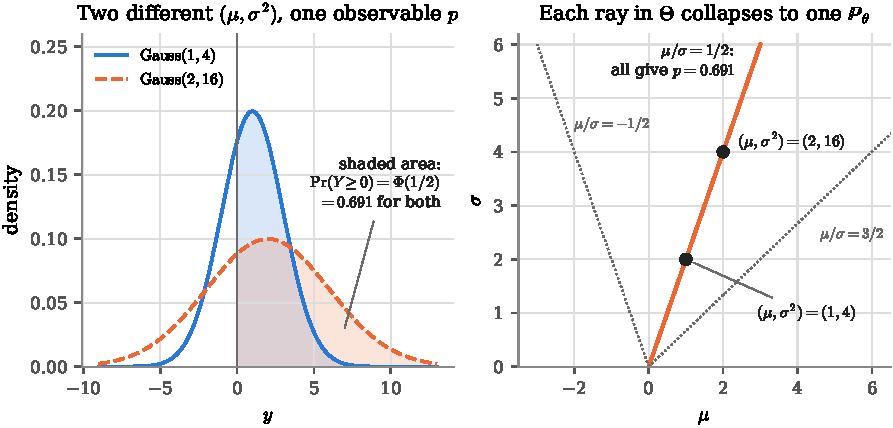
\includegraphics[width=\textwidth]{fig_identifiability}
\caption{\Cref{ex:nonidentifiable}. Left: the densities of $\Gauss(1, 4)$ and $\Gauss(2, 16)$, each with its mass above zero shaded. Right: the $(\mu, \sigma)$ plane, with the ray $\mu/\sigma = 1/2$ in orange, the counterexample's two points marked, and two other rays dotted.}
\label{fig:identifiability}
\end{figure}

\subsection{More examples}

Three variations are worth doing in your head because the pattern is always the same: write down the distribution of what you actually observe as a function of $\theta$, and ask whether that function is one-to-one.

\begin{example}[Censored Exponential]
\label{ex:censored-expo}
Let $X \sim \Expo(\lambda)$ with $\lambda > 0$ unknown, and suppose you observe only $Y = \ind(X > 5)$, a censored version of $X$: you can't see $X$, only whether it exceeded $5$.
Then $Y \sim \Bern(f(\lambda))$ with $f(\lambda) = \Pr(X > 5) = \int_5^\infty \lambda e^{-\lambda x} \, \mathrm{d}x = e^{-5\lambda}$.
The model for $Y$ is $\left( \{0,1\}, (\Bern(e^{-5\lambda}))_{\lambda > 0} \right)$, and $\lambda$ \textit{is} identifiable because $\lambda \mapsto e^{-5\lambda}$ is strictly decreasing, hence injective: from $p = \Pr(Y = 1)$ you recover $\lambda = -\ln(p)/5$.
Censoring loses information (you'll estimate $\lambda$ less precisely than from the $X$'s), but it doesn't lose identifiability.
Compare \cref{ex:nonidentifiable}, where the trouble was not the censoring but the two-dimensional parameter behind a one-dimensional observable.
\end{example}

\begin{example}[Squaring a uniform]
Let $X_i = Y_i^2$ where $Y_1, \ldots, Y_n \iid \text{Unif}([0, a])$ are unobserved.
Is $a$ identifiable?
Yes: $X_i$ takes values in $[0, a^2]$, and $\Pr(X_i \leq x) = \Pr(Y_i \leq \sqrt{x}) = \sqrt{x}/a$ for $0 \leq x \leq a^2$.
Different $a$ give different CDFs (for instance, different supports), so the map $a \mapsto \Pr_a$ is injective.
\end{example}

\begin{example}[Thresholding a uniform at half its range]
Let $X_i = \ind(Y_i \geq a/2)$ where $Y_1, \ldots, Y_n \iid \text{Unif}([0, a])$ are unobserved.
Is $a$ identifiable?
No: $\Pr(Y_i \geq a/2) = 1/2$ for \textit{every} $a > 0$, so $X_i \sim \Bern(1/2)$ whatever $a$ is.
The map $a \mapsto \Pr_a$ is constant, the worst possible failure of injectivity: the data carry no information about $a$ at all.
\end{example}

\Cref{fig:identmaps} draws the three maps side by side; identifiability is the shape of the curve.
In each example the observation is a Bernoulli whose parameter $p$ is a function of $\theta$.
On the left, the censored Exponential has $p = e^{-5\lambda}$, strictly decreasing, so each $p$ comes from exactly one $\lambda$.
In the middle, the uniform thresholded at half its range has $p = \frac12$ for every $a$, so the observation says nothing about $a$.
On the right, the Gaussian sign example has $p = \Phi(\mu/\sigma)$, drawn against $\mu$ for three values of $\sigma$: one value of $p$ is reached by a whole ray of $(\mu, \sigma)$ pairs, the ray of \cref{fig:identifiability}.
Identifiable means the curve never takes the same value twice.

\begin{figure}[htbp]
\centering
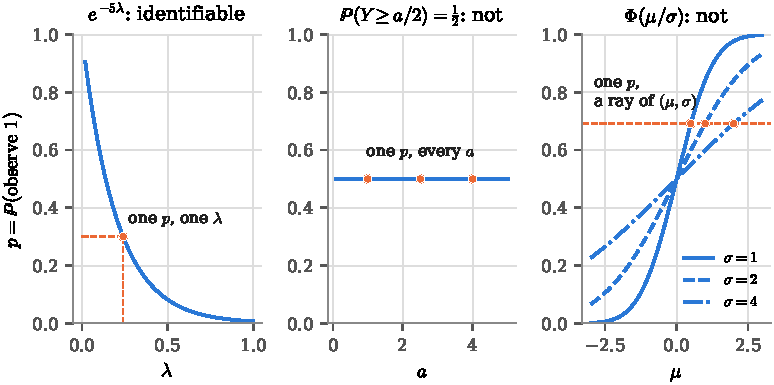
\includegraphics[width=\textwidth]{fig_identifiable_maps}
\caption{The observable Bernoulli parameter $p$ as a function of $\theta$. Left: the censored Exponential, $p = e^{-5\lambda}$. Middle: the uniform thresholded at half its range, $p = \frac12$. Right: the Gaussian sign example, $p = \Phi(\mu/\sigma)$ against $\mu$, one line style per $\sigma$.}
\label{fig:identmaps}
\end{figure}

\begin{bridge}[collinearity, a non-identifiability you have already met]
In a regression course, if two predictors are perfectly collinear (say $x_2 = 2x_1$), the software drops one of them or leaves its coefficient blank.
That is non-identifiability.
The model $Y = \beta_1 x_1 + \beta_2 x_2 + \epsilon$ with $x_2 = 2x_1$ produces exactly the same distribution of $Y$ for every $(\beta_1, \beta_2)$ with the same value of $\beta_1 + 2\beta_2$: a whole line of parameter vectors, one distribution, exactly like the ray in \cref{fig:identifiability}.
The data can tell you $\beta_1 + 2\beta_2$ and nothing more, and no sample size fixes it.
Dropping a predictor is the software's way of choosing one point on the line.
\Cref{ch:regression-multi} returns to this when it needs the design matrix to have full rank.
\end{bridge}

\section{Gaussian mixture models}
\label{sec:models-gmm}

A mixture of Gaussians is best described in terms of the generative model.
You first generate a discrete variable that determines which of the component Gaussians to use, and then generate an observation from that chosen Gaussian density.

More formally, suppose you have two Gaussian r.v.s, $X^{(1)}$ and $X^{(2)}$, such that $X^{(1)} \sim \Gauss(\mu_1, \sigma^2_1)$ and $X^{(2)} \sim \Gauss(\mu_2, \sigma^2_2)$.
Their PDFs are:
\begin{align*}
f_1(x) &= \frac{1}{\sigma_1 \sqrt{2 \pi}} \exp \left( - \frac{(x-\mu_1)^2}{2 \sigma_1^2} \right), \\
f_2(x) &= \frac{1}{\sigma_2 \sqrt{2 \pi}} \exp \left( - \frac{(x-\mu_2)^2}{2 \sigma_2^2} \right).
\end{align*}
Let $\pi \in (0, 1)$ be the \textit{mixture weight}.
A \textbf{mixture} of the two Gaussians has the PDF:
\begin{align*}
f(x) &= \pi f_1(x) + (1 - \pi) f_2(x) \\
	&= \pi \left( \frac{1}{\sigma_1 \sqrt{2 \pi}} \right) \exp \left( - \frac{(x-\mu_1)^2}{2 \sigma_1^2} \right)  + (1-\pi) \left( \frac{1}{\sigma_2 \sqrt{2 \pi}} \right) \exp \left( - \frac{(x-\mu_2)^2}{2 \sigma_2^2} \right).
\end{align*}
(The symbol $\pi$ does double duty here, as the weight and as the constant $3.14159\ldots$ inside the normalizing constants; both uses are standard and the context always tells them apart.)

To better understand a mixture of Gaussian distributions, think of it as a latent variable model.\footnote{Recall that a latent variable is an unobserved variable that can only be inferred indirectly from observable variables.}
Proceed in 3 steps:
\begin{enumerate}
\item \textbf{Latent component selection:} Sample $Z \sim \Bern(\pi)$, so $Z = 1$ with probability $\pi$ and $Z = 0$ with probability $1 - \pi$.
\item \textbf{Independent sampling:} Sample $X^{(1)} \sim \Gauss(\mu_1, \sigma_1^2)$ and $X^{(2)} \sim \Gauss(\mu_2, \sigma_2^2)$, independent of $Z$ and of each other.
Both values are conceptually sampled regardless of $Z$'s value.
\item \textbf{Mixture realization:} Define the r.v.\ $X$ by:
\[
X = Z X^{(1)} + (1 - Z) X^{(2)}.
\]
Only one of the two is used: $X = X^{(1)}$ if $Z = 1$ and $X = X^{(2)}$ if $Z = 0$.
\end{enumerate}

\textbf{Question:} How can this be a \textit{mixture} if each sample comes from exactly \textit{one} Gaussian?

\textbf{Answer:} The answer lies in distinguishing between:
\begin{itemize}[nosep]
\item \textbf{Sample generation}: Each individual observation is generated from only one component, determined by $Z$.
\item \textbf{Distribution properties}: The overall probability distribution of $X$ is a weighted mixture of both Gaussians because you don't get to see $Z$.
\end{itemize}
Mathematically, for any possible value $x$, the law of total probability over $Z$ gives the density
\[
f(x) = \Pr(Z = 1) f_1(x) + \Pr(Z = 0) f_2(x) = \pi f_1(x) + (1-\pi) f_2(x),
\]
so both components contribute to the overall distribution, weighted by their probabilities.
From the population perspective, if you generate $n$ samples from this model, approximately $n\pi$ of them come from $\Gauss(\mu_1, \sigma_1^2)$ and approximately $n(1 - \pi)$ from $\Gauss(\mu_2, \sigma_2^2)$.
\Cref{fig:gmm} shows both perspectives.
On the left, the mixture density is the sum of the two weighted components.
On the right, each of the $400$ draws came from exactly one component, and its color records which; the black mixture density over the histogram is what you see when you cannot tell.

\begin{figure}[htbp]
\centering
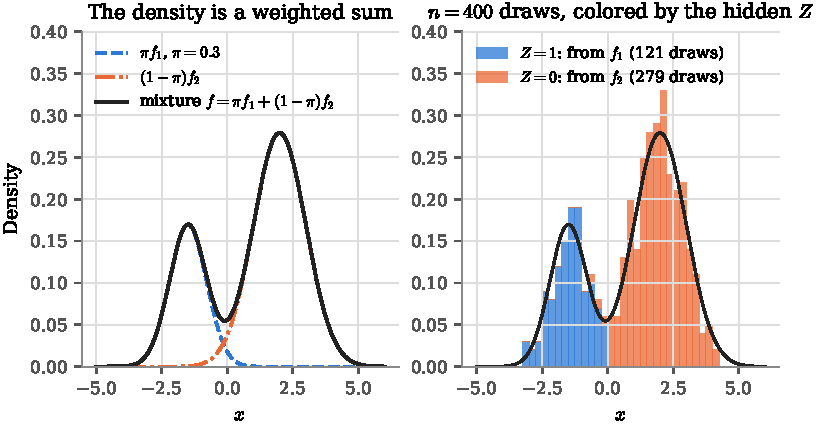
\includegraphics[width=\textwidth]{fig_gaussian_mixture}
\caption{A two-component Gaussian mixture with $\pi = 0.3$, $\Gauss(-1.5, 0.5)$ (blue) and $\Gauss(2, 1)$ (orange). Left: the two weighted components and their sum, the mixture density (black). Right: $400$ draws, histogrammed and colored by the latent $Z$, with the mixture density over them.}
\label{fig:gmm}
\end{figure}

An alternative specification of the same r.v.\ is $X = (X^{(1)})^Z (X^{(2)})^{1-Z}$, which picks the same component as before.
The latent variable perspective is especially useful for inference algorithms like EM (expectation-maximization), where you need to estimate both the component parameters $(\mu_1, \sigma_1^2, \mu_2, \sigma_2^2)$ and the mixture weight $\pi$ without ever observing which component produced which observation.

\begin{bridge}[a histogram with two peaks]
An introductory course reads a histogram with two peaks as a sign that the data may mix two groups, and suggests separating them if some variable records the group.
The Gaussian mixture is that reading as a model, for when no variable does: $Z$ is the unrecorded group, each component is the distribution within one group, and $\pi$ is the share of the first group.
With the groups recorded, $\pi$ would be estimated by the proportion of observations in the first group, a sample proportion like $\hat{p}$, and each component from its own group's mean and variance.
Without them, \cref{sec:lik-em} estimates all five parameters at once; for the waiting times between eruptions of the Old Faithful geyser, with peaks near $55$ and $80$ minutes, it puts about a third of the waits in the short group.
\end{bridge}

\subsection{Possible Gaussian mixture models}

There are several scenarios for a model with mixtures of Gaussians, depending on the constraints imposed on its 5 parameters.
Here are 3 possible examples.
It should be noted that, for clarity but with an abuse of notation, the PDFs of the two Gaussian r.v.s are not explicitly written below; each distribution is written generically as $\Gauss(\mu_1, \sigma_1^2)$.
\begin{enumerate}
\item Model where all 5 parameters are unknown:
\[
\left( \real, (\pi \cdot \Gauss(\mu_1, \sigma_1^2) + (1-\pi) \cdot \Gauss(\mu_2, \sigma_2^2))_{\pi \in (0,1), \, \mu_1, \mu_2 \in \real, \, \sigma_1^2, \sigma_2^2 \in (0,\infty)} \right).
\]
\item Model with known variances, and for simplicity suppose $\sigma_1^2 = \sigma_2^2 = 1$:
\[
\left( \real, (\pi \cdot \Gauss(\mu_1, 1) + (1-\pi) \cdot \Gauss(\mu_2, 1))_{\pi \in (0,1), \, \mu_1, \mu_2 \in \real} \right).
\]
\item Model with only unknown means, and for simplicity suppose $\sigma_1^2 = \sigma_2^2 = 1$ and $\pi = 1/2$:
\[
\left( \real, \left( \tfrac{1}{2} \cdot \Gauss(\mu_1, 1) + \tfrac{1}{2} \cdot \Gauss(\mu_2, 1) \right)_{\mu_1, \mu_2 \in \real} \right).
\]
\end{enumerate}

\begin{pitfall}[mixtures are identifiable only up to relabeling]
Take the third model and the two parameter vectors $(\mu_1, \mu_2) = (-1, 2)$ and $(\mu_1, \mu_2) = (2, -1)$.
They're different points of $\Theta = \real^2$, and they give exactly the same density: $\frac12 f_{-1} + \frac12 f_{2} = \frac12 f_{2} + \frac12 f_{-1}$.
So by \cref{def:identifiable} the parameter is not identifiable; the same happens in the first two models with $(\pi, \mu_1, \sigma_1^2, \mu_2, \sigma_2^2) \leftrightarrow (1-\pi, \mu_2, \sigma_2^2, \mu_1, \sigma_1^2)$.
This failure is called \textit{label switching}, and it's harmless in a way \cref{ex:nonidentifiable} is not: the two parameter vectors describe the same two components with their names swapped, so the data do pin down the components, just not which one is `first'.
The fix is a convention such as $\mu_1 < \mu_2$, which restricts $\Theta$ to half the plane and removes the swap; that nothing else collides, so that the map is then injective, is a theorem about finite Gaussian mixtures that is not proved here.
The lesson is that non-identifiability is sometimes a defect of the labeling rather than of the information in the data, and the first thing to ask when you find it is which of the two you're looking at.
\end{pitfall}

\section{What comes next}
\label{sec:models-next}

A model fixes the family of candidate distributions.
Three things are done inside it, and they are Part III: guess $\theta$ (\cref{ch:estimators}), attach a range to the guess (\cref{ch:confidence-intervals}), and decide a yes/no question about $\theta$ (\cref{ch:tests-foundations}).
All three are stated for a general model $(E, (\Pr_\theta)_{\theta \in \Theta})$ and computed, as always, for the kiss model.
All three also rest on what an average of $n$ draws does as $n$ grows, and that is Part II, which comes first: where the average settles (\cref{ch:lln}), how it fluctuates on the way (\cref{ch:clt}), what may be done to those limits (\cref{ch:limit-tools}), and the Gaussian distribution the limits land on (\cref{ch:gaussian}).

\section{Summary}
\label{sec:models-summary}

\begin{itemize}[nosep]
\item A statistical model is $\left( E, (\Pr_\theta)_{\theta \in \Theta} \right)$: a sample space and a family of candidate distributions for $X$, indexed by a parameter. Parameters define distributions; learning one is learning the other. The sample space must not depend on $\theta$.
\item Assumptions buy fewer parameters: the siblings PMF has six, the shifted Poisson one. The price is misspecification if the assumption is wrong.
\item Three layers: the sample space $\Omega$ (every complete outcome), random variables (functions on $\Omega$, the measuring instruments and the rules applied to their readings), and the observations (those functions evaluated at the one outcome that happened). An estimate is one draw from the estimator's distribution. Inference does not invert the chain; it holds the one value up against the distribution of the rule. For fixed $n$, take $\Omega = E^n$.
\item Well-specified: the true $\Pr$ is some $\Pr_{\theta^*}$ in the family. Everything from Part III on assumes this; \cref{ch:distances} says what estimators estimate when it fails.
\item Parametric: $\Theta \subseteq \real^d$. Nonparametric: $\Theta$ is a space of functions. Semiparametric: a finite-dimensional parameter of interest plus an infinite-dimensional nuisance parameter.
\item Identifiable: $\theta \mapsto \Pr_\theta$ is injective, so knowing the distribution of the data would tell you $\theta$. To show a parameter is not identifiable, exhibit two parameter values with the same distribution. Observing only a function of the data can destroy identifiability (two numbers behind one observable proportion) or leave it intact (one number behind one proportion, injectively); what matters is whether the map from the parameter to the observable distribution is one-to-one.
\item A Gaussian mixture is a latent-variable model: pick a component with $Z \sim \Bern(\pi)$, then draw from it. Its density is $\pi f_1 + (1-\pi) f_2$. Its parameter is identifiable only up to swapping the component labels.
\end{itemize}

\section{Exercises}
\label{sec:models-exercises}

\begin{exercise}
Which of the following is a statistical model? (1) $\left( \{1\}, (\Bern(p))_{p \in (0,1)} \right)$; (2) $\left( \{0,1\}, (\Bern(p))_{p \in (0.2, 0.4)} \right)$; (3) both; (4) neither.
\end{exercise}
\begin{solution}
(2). The first has a sample space that excludes the outcome $0$, which every $\Bern(p)$ puts mass on. The second is a legitimate model with a restricted parameter space; whether it's well-specified is a separate question.
\end{solution}

\begin{exercise}
Let $\Xton \iid \text{Unif}([0, a])$ for some unknown $a > 0$. Which is the associated statistical model: (1) $\left( [0, a], (\text{Unif}([0,a]))_{a > 0} \right)$; (2) $\left( \real_+, (\text{Unif}([0,a]))_{a > 0} \right)$; (3) $\left( \real, (\text{Unif}([0,a]))_{a > 0} \right)$; (4) none?
\end{exercise}
\begin{solution}
The intended answer is (2), and (1) is the one that is definitely wrong: the sample space can't depend on the unknown $a$. Both $\real_+$ and $\real$ contain every observation for every $a$, so by \cref{def:statmodel} (3) is a legitimate model too; the convention is to take $E = \real_+$, the smallest natural set that works, and that convention is what the question is testing.
\end{solution}

\begin{exercise}
Which of these models are parametric? (A) $E = \{0, 1, 2, \ldots\}$ and $\{\Pr_\theta\}$ is the set of all distributions on $E$. (B) $E = \{0,1\}$, $(\Bern(\theta))_{\theta \in [0,1]}$. (C) $E = \real$, $(\Gauss(0, \sigma^2))_{\sigma^2 > 0}$. (D) $E = \{1,2,3,4\}$ and $\Pr_{(p_1, \ldots, p_4)}$ puts probability $p_i$ on $i$, with $p_i \geq 0$ and $\sum p_i = 1$. (E) $E = \real$, $(\Gauss(\mu, \sigma^2))_{\mu \in \real, \sigma^2 > 0}$. (F) $E = [0, \infty)$, $(\text{Unif}([0, \theta]))_{\theta > 0}$. (G) $E = [0,1]$ and $\{\Pr_f\}$ is the set of all distributions with a continuous density $f$ on $[0,1]$.
\end{exercise}
\begin{solution}
B, C, D, E, F. In (A) a member of the family needs infinitely many numbers (a probability for every non-negative integer). (B), (C), (F) need one number, (E) two, (D) three (the fourth $p_i$ is determined by the other three). In (G) a member is a continuous function on $[0,1]$, which no finite list of numbers specifies.
\end{solution}

\begin{exercise}
You observe $X_i = \ind(Y_i \geq c)$ for $Y_i \iid \Gauss(\mu, 1)$ with $\sigma^2 = 1$ known and $c$ a known constant. Is $\mu$ identifiable? What if instead $\sigma^2$ is unknown and $\mu = 0$ is known?
\end{exercise}
\begin{solution}
$\Pr(Y_i \geq c) = 1 - \Phi(c - \mu) = \Phi(\mu - c)$, strictly increasing in $\mu$, so $\mu$ is identifiable: $\mu = c + \Phi^{-1}(p)$. With $\mu = 0$ known and $\sigma$ unknown, $\Pr(Y_i \geq c) = \Phi(-c/\sigma)$: for $c \neq 0$ this is strictly monotone in $\sigma$ and $\sigma$ is identifiable; for $c = 0$ it equals $1/2$ for every $\sigma$, and $\sigma$ is not. The threshold matters: thresholding at the known mean throws away all information about the spread, as in the uniform example.
\end{solution}

\begin{exercise}
In the two-component mixture with all five parameters unknown, is the parameter $(\pi, \mu_1, \sigma_1^2, \mu_2, \sigma_2^2)$ identifiable on the restricted parameter space where $\mu_1 < \mu_2$? What about the point $\pi = 1$, if it were allowed?
\end{exercise}
\begin{solution}
Ordering the means removes the label-switching ambiguity, and it's a theorem (not proved here) that finite Gaussian mixtures are then identifiable. The endpoint $\pi = 1$ is excluded from $\Theta$ for a good reason: at $\pi = 1$ the density is $f_1$ whatever $(\mu_2, \sigma_2^2)$ are, so every value of the second component's parameters gives the same distribution. A component with zero weight is invisible, which is why the weight is required to be in the open interval $(0, 1)$.
\end{solution}


\partintro{The three questions of \cref{ch:kiss} are about the random variable $\bar{R}_n$ as $n$ grows, and `as $n$ grows' is a limit. This part has the three limit facts every later chapter uses, the Law of Large Numbers (\cref{ch:lln}), the Central Limit Theorem (\cref{ch:clt}) and the rules for working with limits (\cref{ch:limit-tools}), and then the Gaussian distribution and the quantile notation that the rest of the book is written in (\cref{ch:gaussian}). If limits are not your difficulty, \cref{ch:lln}'s opening box says what can be skipped.}
\part{Probability for Statistics}
\chapter{The Law of Large Numbers}
\label{ch:lln}

\begin{chaptergoals}
\begin{itemize}[nosep]
\item Why limits of random variables need different tools than limits of numbers.
\item The sample mean on two scales: collapsing on $\mu$ (this chapter) and, magnified by $\sqrt{n}$, settling into a Gaussian (the next).
\item Convergence in probability, the mode of convergence that says an estimator gets close to what it estimates.
\item The Weak Law of Large Numbers, with Chebyshev's inequality as the proof.
\end{itemize}
The running example is the kiss experiment of \cref{ch:kiss}: $n = 124$ couples, $80$ of whom turned right, so $\hat{p} = \bar{R}_n = 0.645$.

\Cref{ch:models} fixed the object inference happens in; this part supplies the three facts about averages that Part III stands on.

\textbf{The next three chapters.}
The rest of the book rests on three limit facts about averages: the Law of Large Numbers (averages settle on their expectations, this chapter), the Central Limit Theorem (the error of an average is Gaussian on the $1/\sqrt{n}$ scale, \cref{ch:clt}), and the rules for transforming limits and plugging in estimates (continuous mapping, Slutsky, the delta method, \cref{ch:limit-tools}).
Those three chapters are the minimal path.
Two more modes of convergence, almost sure and in mean, complete the standard hierarchy; that material is in \cref{app:modes} because nothing later is proved with it; where a later chapter mentions almost sure convergence, the in-probability version is the one in use.
Read it once for orientation and don't spend time mastering it.
\end{chaptergoals}

\begin{intuition}[what `asymptotic' means]
An asymptotic result is a license to replace an unknown sampling distribution by its limiting distribution, usually a Gaussian, with an error the theorem does not tell you.
That is all `asymptotic' ever means in this book.
The definitions below are about infinite sequences, while every application is about one fixed sample size, usually $n = 124$; the theorems say $n \to \infty$ and they get applied at $n = 64$ without further comment.
The gap is real, and \cref{sec:conv-what-limits-buy} in the next chapter says what the alternatives are and why statistical practice accepts the trade.
When a later chapter says `by the CLT' or `asymptotically normal', read it as: for the $n$ at hand, treat this as Gaussian and carry on.
\end{intuition}

\section{Why limits of random variables need new tools}
\label{sec:conv-why}

\Cref{ch:kiss} asked whether $\hat{p}$ is close to $p$ once $n$ is large.
That is a question about a limit, and limits of random variables need their own definition.
In calculus you say that a sequence of real numbers $x_n$ converges to a limit $x$ if, for any $\epsilon > 0$, $\abs{x_n - x} < \epsilon$ for all large $n$ \toolkit{sec:math-limits}.
Convergence is more subtle in probability.
Returning to calculus, suppose that $x_n = x$ for all $n$.
Then, trivially, $\ds \lim_{n \to \infty} x_n = x$.

Consider a probabilistic version of this example.
Suppose that $X_1, X_2, \ldots$ is a sequence of i.i.d.\ r.v.s such that $X_i \iid \Gauss(0,1)$.
Since these all have the same distribution, you might think $X_n$ `converges' to $X \sim \Gauss(0,1)$.
But this can't be right: $X_n - X \sim \Gauss(0, 2)$ for every $n$, so $\Pr(\abs{X_n - X} < \epsilon)$ is the same small number for every $n$ and never improves. (In fact $\Pr(X_n = X) = 0$ for all $n$, since two independent continuous r.v.s are equal with probability zero.\footnote{Why is this true? Let $Y_1$ and $Y_2$ be continuous r.v.s with joint density $f_{Y_1, Y_2}$. Then
\[
\Pr(Y_1 = Y_2) = \iint_D f_{Y_1, Y_2}(y_1, y_2) \, \mathrm{d}y_1 \, \mathrm{d}y_2, \qquad D = \{(y_1,y_2) \in \real^2: y_1 = y_2 \}.
\]
The set $D$ is a line living in two dimensions and hence has no area: you're integrating a bounded function over a region of zero area, so the integral is $0$.
This is the two-dimensional version of the fact that the `area' under a density at a single point is zero.})
This suggests limiting processes involving probabilities require different tools than those limiting processes from calculus.

The central ideas in this chapter and the next are the two most famous results in all of probability theory: the Law(s) of Large Numbers and the Central Limit Theorem.
An understanding of why these results are valid requires an understanding of limiting processes that involve r.v.s.
These limits are conceptually more general than the limits of undergraduate calculus since, as limits of r.v.s, these limits are not limits of numbers but limits of \textit{functions}.

So what is meant by `convergence of random variables'?
And what is a sequence of r.v.s?
Recall that, by definition, an r.v.\ is a mapping from a sample space, $S$, to the real number line \toolkit{sec:math-rv}.
Suppose, to fix ideas, that the outcomes can be listed (a continuous r.v.\ needs a richer sample space, but the picture is the same), so you can write:
\[
S = \{ s_1, \ldots, s_k \}.
\]

This means an r.v.\ $X$ defined on $S$ can be written as:
\[
X(s_i) = x_i, \text{ for } i = 1,\ldots,k.
\]

When you have a sequence of r.v.s it's useful to keep in mind that there's always an underlying sample space.
In particular, each $X_n$ is a function from $S$ to $\real$:
\[
X_n(s_i) = x_{n,i}, \text{ for } i = 1,\ldots,k.
\]

So a sequence of r.v.s is a sequence of functions $X_n: S \to \real$.
Pick an outcome $s_i$ and you get an ordinary sequence of numbers $x_{1,i}, x_{2,i}, x_{3,i}, \ldots$, one such sequence for every outcome.
A \textit{realization} of the sequence is what you see when the experiment is run once and the outcome happens to be $s_i$.

\begin{figure}[htbp]
\centering
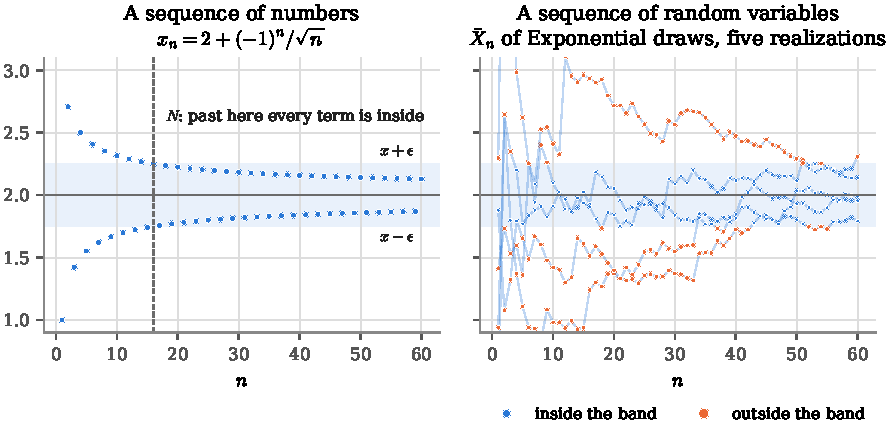
\includegraphics[width=\textwidth]{fig_sequence_vs_random}
\caption{Left: a sequence of numbers converging to $2$. For the band of half-width $\epsilon$ there is an index $N$ past which every term is inside. Right: five realizations of the running sample mean $\bar{X}_n$ of Exponential draws with mean $2$, one path per outcome of the experiment. Each path eventually settles inside the band, but at a different index, and no $N$ works for every path: some realization will leave the band after any $N$ you name. The modes of convergence are different ways of saying `the orange points become rare.'}
\label{fig:seqrand}
\end{figure}

This chapter and the next examine the two modes of convergence this book works with; \cref{app:modes} has the full set.
Why are there different modes of convergence?
Remember that to say a sequence $(X_i)_{i=1}^{\infty}$ converges to $X$ means that the $X_i$'s are getting `closer and closer' to $X$.
Different modes of convergence relate to different ways of defining what `closer' means.
\Cref{fig:seqrand} shows the difficulty: for a sequence of numbers there is a single index $N$ past which every term is within $\epsilon$ of the limit, while for a sequence of r.v.s the index that works depends on the outcome of the experiment and may not exist for some outcomes.

Two of the modes, convergence almost surely and convergence in probability, compare the \textit{values} of $X_n$ and $X$ outcome by outcome, so $X_n$ and $X$ must live on the same sample space.
The third, convergence in distribution, compares the CDFs of $X_n$ and $X$ and never looks at values at all; $X_n$ and $X$ can be defined on entirely different probability spaces.
But as r.v.s have CDFs, the difference between sequences of r.v.s and sequences of CDFs isn't as significant as you might expect.

So it's important to emphasize here that the `things' converging are r.v.s, or their CDFs, and that they converge to an r.v., or a CDF.\footnote{Just because a sequence of r.v.s converges to an r.v.\ doesn't mean the limiting r.v.\ has an interesting distribution or what you normally think of as a `distribution'.
In fact, one mode of convergence explained below (convergence in probability), is almost entirely concerned with the convergence of sequences of r.v.s to a constant or `degenerate' r.v.}

\section{A first look: the sample mean on two scales}
\label{sec:conv-two-scales}

To motivate the notion of convergence of r.v.s, consider the following example.
Suppose that $\Xton$ are i.i.d.\ r.v.s with mean $\mu$ and variance $\sigma^2$ and define the (theoretical, non-realized) sample mean:
\[
\bar{X}_n = \frac{1}{n} \sum_{i=1}^n X_i.
\]

First, consider the behavior of the distribution of $\bar{X}_n$ when $n$ is large.
It seems reasonable that $\bar{X}_n$ will be close to $\mu$ if $n$ is sufficiently large;
that is, the r.v.\ $\bar{X}_n - \mu$ should have a distribution that, for large $n$, is concentrated around 0 or, more precisely:
\[
\Pr(\abs{\bar{X}_n - \mu} \leq \epsilon) \approx 1,
\]

for any small positive number $\epsilon$.
This type of limiting process, and more specifically, that as $n$ increases without limit the probability equals 1, is an example of \textit{convergence in probability}, and also illustrates a convergence process to a constant (here, $\mu$), as discussed in the previous footnote.

Moreover because $\var( \bar{X}_n ) = \sigma^2/n$,\footnote{That $\var( \bar{X}_n ) = \sigma^2/n$ follows from the properties of the variance and the independence of the $X_i$.
Specifically:
\[
\var(\bar{X}_n) = \frac{1}{n^2} \var(X_1 + \cdots + X_n) = \frac{n \sigma^2}{n^2} = \frac{\sigma^2}{n}.
\]} it follows that $\var( \bar{X}_n ) \to 0$ as $n \to \infty$.
Because the variance of $\bar{X}_n$ eventually vanishes as $n$ increases, the limit tells you nothing about the \textit{shape} of the distribution of $\bar{X}_n$: every density in the left panel of \cref{fig:twoviews} is on its way to becoming a spike at $\mu$.

It's possible though to look at the difference between $\bar{X}_n$ and $\mu$ on a `magnified' scale.
To that end, multiply the difference $\bar{X}_n - \mu$ by $\sqrt{n}$, which makes the mean and variance of the resulting r.v.\ constant.
Specifically, define the r.v.\ $Y_n$ by:
\[
Y_n = \sqrt{n}(\bar{X}_n - \mu),
\]

and note that:
\[
\E[Y_n] = \E[\sqrt{n}(\bar{X}_n - \mu)] = \sqrt{n} (\E[\bar{X}_n] - \mu) = \sqrt{n} (\mu - \mu) = 0,
\]

and
\[
\var(Y_n) = \var(\sqrt{n}(\bar{X}_n - \mu)) = n \var(\bar{X}_n - \mu) = n \var(\bar{X}_n) = \sigma^2.
\]

\begin{intuition}[what's special about $\sqrt{n}$?]
Why does multiplying by $\sqrt{n}$, and not by $n$ or by $\log n$, yield a constant mean and variance?
\begin{itemize}[nosep]
\item \textbf{The mean:} Multiplying $\bar{X}_n - \mu$ by anything doesn't impact its expected value because $\bar{X}_n$ is an unbiased estimator of $\mu$, so the expected value of the difference is $0$ to begin with.
\item \textbf{The variance:} As $n$ increases, $\var(\bar{X}_n) = \sigma^2/n$ decreases.
When you multiply an r.v.\ by $\sqrt{n}$ the variance is scaled by a factor of $n$, which exactly cancels the division by $n$.
Multiplying by $n$ instead would scale the variance by $n^2$ and the result would blow up; multiplying by $\log n$ would not be enough and the result would still collapse to a spike.
\end{itemize}
The standard deviation of $\bar{X}_n$ is $\sigma/\sqrt{n}$, so $\sqrt{n}$ is the magnification that holds the spread fixed.
\end{intuition}

\begin{figure}[htbp]
\centering
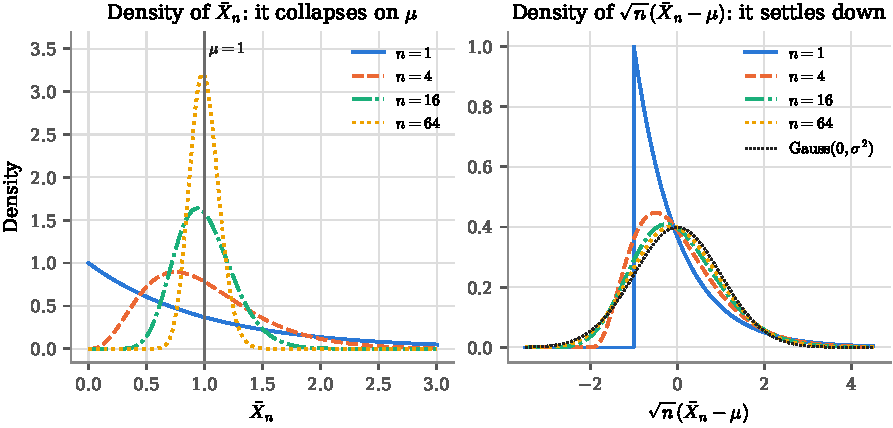
\includegraphics[width=\textwidth]{fig_lln_clt_two_views}
\caption{The same sample mean of $\Expo(1)$ draws on two scales. Left: the density of $\bar{X}_n$ collapses onto $\mu = 1$ as $n$ grows (this is the Law of Large Numbers). Right: after the $\sqrt{n}$ magnification the density of $\sqrt{n}(\bar{X}_n - \mu)$ keeps a fixed spread and its shape settles down to a Gaussian (this is the Central Limit Theorem). At $n = 1$ the magnified density is the skewed exponential itself, shifted; by $n = 64$ it is hard to tell from $\Gauss(0, \sigma^2)$.}
\label{fig:twoviews}
\end{figure}

You can now consider the behavior of the CDF of $Y_n$ as $n$ increases.
If this sequence of CDFs has a limit, then you can use the limiting CDF to approximate the CDF of $Y_n$ (and hence of $\bar{X}_n$).

For example, suppose you have that:
\[
\Pr(Y_n \leq y) = \Pr( \sqrt{n}(\bar{X}_n - \mu) \leq y) \approx F_0(y).
\]

Then, to say something about the CDF of $\bar{X}_n$, subtract $\mu$ from $\bar{X}_n$ and multiply this difference by $\sqrt{n}$, to get:
\[
\Pr(\bar{X}_n \leq x) = \Pr( \sqrt{n}(\bar{X}_n - \mu)  \leq \sqrt{n}(x - \mu)) \approx F_0(\sqrt{n}(x - \mu)),
\]

provided $n$ is sufficiently large to make the approximation valid.
This type of limiting process is an example of \textit{convergence in distribution}, which is the subject of \cref{ch:clt}.

What if instead of transforming $\bar{X}_n$ into $Y_n$, you `standardized' it by dividing $Y_n$ by $\sigma$.
That is, define the r.v.\ $Z_n$ by:
\[
Z_n = \sqrt{n} \left( \frac{\bar{X}_n - \mu}{\sigma} \right).
\]

Now, calculate $\E[Z_n]$ and $\var(Z_n)$:
\[
\E[Z_n] = \E \left[ \sqrt{n} \left( \frac{\bar{X}_n - \mu}{\sigma} \right) \right] = \frac{\sqrt{n}}{\sigma} (\E[\bar{X}_n] - \mu) = \frac{\sqrt{n}}{\sigma} (\mu - \mu) = 0.
\]

Thus, $\E[Y_n] = \E[Z_n] = 0$.
But observe that $\var(Z_n) \neq \var(Y_n) = \sigma^2$:
\begin{align*}
\var(Z_n) &= \var \left( \sqrt{n} \left( \frac{\bar{X}_n - \mu}{\sigma} \right) \right) \\
 &= \frac{n}{\sigma^2} \var \left( \bar{X}_n \right) \\
 &= \frac{n}{\sigma^2} \var \left( \frac{1}{n} \sum_{i=1}^n X_i \right)  \\
 &= \frac{1}{n \sigma^2} \var \left( \sum_{i=1}^n X_i \right) \\
 &= \frac{n \sigma^2}{n \sigma^2} \\
 &= 1.
\end{align*}

Thus, despite the extra scaling factor, $\sqrt{n}$, the r.v.\ $Z_n$ has a `standard' look to it: Its mean is 0 and its variance is 1.
It may not come as a surprise that $Z_n$ converges in distribution to a standard Gaussian distribution.

\begin{bridge}[the standard error]
An introductory course states, usually without proof, that the sampling distribution of the sample mean has mean $\mu$, has standard deviation $\sigma/\sqrt{n}$ (the \textit{standard error} of the mean), and is approximately normal when $n$ is large.
The two panels of \cref{fig:twoviews} are the two halves of that statement.
The standard error shrinking to zero is what drives the Law of Large Numbers.
The shape becoming normal is the Central Limit Theorem.
Dividing $\bar{X}_n - \mu$ by the standard error $\sigma/\sqrt{n}$ is exactly the standardization that produces $Z_n$:
\[
Z_n = \frac{\bar{X}_n - \mu}{\sigma/\sqrt{n}} = \sqrt{n} \left( \frac{\bar{X}_n - \mu}{\sigma} \right).
\]
This chapter proves the first half; \cref{ch:clt} makes `approximately normal when $n$ is large' into a theorem and says what `large' buys you.
\end{bridge}

\section{Convergence in probability}
\label{sec:conv-prob}

Convergence in probability considers the distance between a sequence of r.v.s $X_n$ and some number $x$ being at least as large as some arbitrary $\epsilon > 0$.
That is, in formal terms you're concerned with whether the probability of $\abs{X_n - x} \geq \epsilon$ converges to 0.

A first step in such problems, and limit problems generally, is to grasp the meaning of $\abs{X_n - x} \geq \epsilon$.
An absolute value can be thought of as the distance from 0.
So $\abs{X_n - x}$ is the distance of the number $X_n - x$ from 0, and the event $\abs{X_n - x} \geq \epsilon$ says that this distance is at least $\epsilon$, which happens either when $X_n - x \geq \epsilon$ or when $X_n - x \leq - \epsilon$.
A visualization along the real line is instructive.

\begin{center}
\begin{tikzpicture}[x=1cm, y=1cm]
  \draw[-{Latex[length=2mm]}, gray] (-4.6,0) -- (4.6,0);
  \draw[very thick, boxorange, -{Latex[length=2mm]}] (1.6,0) -- (4.3,0);
  \draw[very thick, boxorange, -{Latex[length=2mm]}] (-1.6,0) -- (-4.3,0);
  \draw[very thick, boxblue] (-1.6,0) -- (1.6,0);
  \fill[boxorange] (1.6,0) circle (2pt);
  \fill[boxorange] (-1.6,0) circle (2pt);
  \draw (0,0.1) -- (0,-0.1);
  \node[below] at (0,-0.1) {$0$};
  \node[below] at (1.6,-0.1) {$\epsilon$};
  \node[below] at (-1.6,-0.1) {$-\epsilon$};
  \node[above, font=\small] at (3.0,0.1) {$X_n - x \geq \epsilon$};
  \node[above, font=\small] at (-3.0,0.1) {$X_n - x \leq -\epsilon$};
  \node[above, font=\small, boxblue!70!black] at (0,0.1) {$\abs{X_n - x} < \epsilon$};
\end{tikzpicture}
\end{center}

If a sequence of r.v.s converges in probability to a number, say, 0, then you say the sequence converges to the zero \textit{random variable} (not the number 0).
Now for the definition.

\begin{definition}[Convergence in probability]
\label{def:convp}
A sequence of r.v.s, $(X_n)_{n \geq 1}$, \textbf{converges in probability} to an r.v.\ $X$ if, for every $\epsilon > 0$:
\[
\lim_{n \to \infty} \Pr(\abs{X_n - X} \geq \epsilon) = 0, \, \text{ or equivalently } \, \lim_{n \to \infty} \Pr(\abs{X_n - X} < \epsilon) = 1.
\]
If $(X_n)_{n \geq 1}$ converges in probability to some r.v.\ $X$, then this is denoted by $X_n \convp X$.
\end{definition}

\begin{inwords}
\textbf{In words.} Read the definition from the inside out. Fix a tolerance $\epsilon$. For each $n$, $\Pr(\abs{X_n - X} \geq \epsilon)$ is a number, the probability mass that $X_n$ puts outside the $\epsilon$-band around $X$. The definition says this sequence of \textit{numbers} goes to $0$ in the ordinary calculus sense \toolkit{sec:math-limits}, and that it must do so for every tolerance, however small. Nothing is said about any single outcome; everything is said about probabilities.
\par\smallskip
\textbf{For the kiss data.} $\bar{R}_n \convp p$ means: pick any tolerance, say $0.01$; the probability that the sample proportion turning right misses $p$ by more than $0.01$ can be made as small as you like by observing enough couples. It does not say how many couples; \cref{sec:wlln} and \cref{ch:clt} do.
\end{inwords}
\Cref{fig:convpband} shows the picture for the sample mean, where $X$ is the constant $\mu$.

\begin{figure}[htbp]
\centering
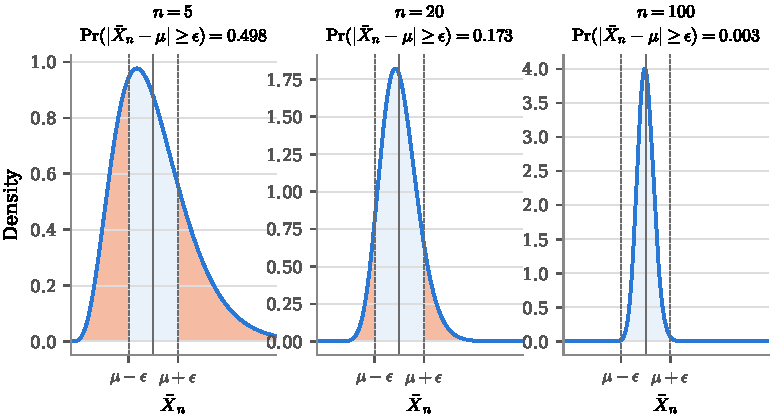
\includegraphics[width=\textwidth]{fig_conv_prob_band}
\caption{Convergence in probability as a picture. The density of $\bar{X}_n$ for $\Expo(1)$ draws at three sample sizes, with the band $[\mu - \epsilon, \mu + \epsilon]$ for $\epsilon = 0.3$. The shaded orange mass is $\Pr(\abs{\bar{X}_n - \mu} \geq \epsilon)$; it goes from about one half at $n = 5$ to essentially zero at $n = 100$. Shrink $\epsilon$ and the same thing happens, only it takes a larger $n$.}
\label{fig:convpband}
\end{figure}

Though convergence in probability is defined as a sequence of r.v.s converging to an r.v., in statistical applications the limit is almost always a constant: the sample mean converges to $\mu$, an estimator converges to the parameter it estimates.
There's a reason the interesting limits are constants.
If the r.v.s in the sequence are independent and the sequence converges in probability, then the limiting r.v.\ must be a constant.\footnote{A sketch, not a proof, and not needed later: the limit of a sequence can't depend on any finite number of its terms (throw away the first million terms and the limit is unchanged). If the terms are independent, the limit is therefore independent of every one of them, hence independent of everything that's random in the experiment, hence independent of itself. An r.v.\ independent of itself satisfies $\var(X) = \cov(X, X) = 0$, so it's a constant. The precise statement is Kolmogorov's zero-one law.}
The sample mean $\bar{X}_n$ isn't a sequence of independent r.v.s (each $\bar{X}_n$ shares $X_1$ with all the others), so this fact doesn't apply to it directly, but the conclusion is the same: the randomness averages out.

\subsection{Example: the minimum of uniforms}

\begin{example}
\label{ex:min-unif}
Let $X_1, X_2, \ldots \iid \text{Unif}([0,1])$ and define the minimum of the first $n$ by $\ds X_{(1)} = \min_{i=1,\ldots,n} X_i$.
Then:
\[
X_{(1)} \convp 0.
\]
\end{example}

\coreproof{Write the event $\abs{X_{(1)} - 0} \geq \epsilon$ as an event about the whole sample, use independence to turn its probability into a product of $n$ equal factors, and let $n \to \infty$. This is the template for every direct convergence proof that follows.}
\begin{proof}
\leavevmode % Puts first item on next line
\begin{itemize}

\item Let $\epsilon > 0$.
Write the claim using the definition of convergence in probability: you need $\Pr(\abs{X_{(1)} - 0} \geq \epsilon) \to 0$.

\item Now, you'll simplify the expression in such a way as to eventually take the limit of the expression as $n \to \infty$.

\item To that end, observe that:
\begin{align*}
\Pr(\abs{X_{(1)} - 0} \geq \epsilon) &= \Pr(\abs{X_{(1)}} \geq \epsilon) \\
								&= \Pr(X_{(1)} \geq \epsilon) \\
								&= \Pr(X_1 \geq \epsilon, X_2 \geq \epsilon, \ldots, X_n \geq \epsilon) \\
								&= \Pr(X_1 \geq \epsilon) \Pr(X_2 \geq \epsilon) \cdots \Pr(X_n \geq \epsilon) \\
								&= \Pr(X_1 \geq \epsilon)^n.
\end{align*}

The movement from the second to the third equality holds because, as $X_{(1)}$ is the minimum of the $X_i$'s, the minimum is at least $\epsilon$ exactly when every $X_i$ is at least $\epsilon$: the single event is equivalent to the joint event.
The fourth equality results since the $X_i$'s are independent, and the fifth since they're identically distributed.

\item You know that $X_1 \sim \text{Unif}([0,1])$.
Therefore, $f_{{X}_1}(x) = 1$ for all values in $X_1$'s support.

\item This implies that $\ds \Pr(X_1 \geq \epsilon) = \int_{\epsilon}^1 1 \dx = 1 - \epsilon$, and further that:
\[
\Pr(X_1 \geq \epsilon)^n = (1 - \epsilon)^n.
\]

Also, note that $1 - \epsilon$ is some number between 0 and 1 (for $\epsilon \geq 1$ the probability is already $0$, so there's nothing to prove).

\item Now you're ready to take the limit of this probability and confirm the statement:
\[
\lim_{n \to \infty} \Pr(\abs{X_{(1)} - 0} \geq \epsilon) = \lim_{n \to \infty} (1 - \epsilon)^n = 0,
\]

and hence $X_{(1)} \convp 0$, as desired.
\end{itemize}
\end{proof}

\begin{figure}[htbp]
\centering
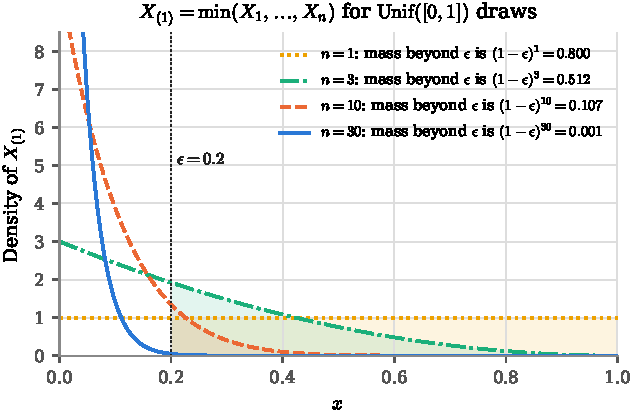
\includegraphics[width=0.8\textwidth]{fig_min_uniform}
\caption{\Cref{ex:min-unif} as a picture. The density of $X_{(1)} = \min(X_1, \ldots, X_n)$ is $n(1-x)^{n-1}$ on $[0,1]$. As $n$ grows the mass piles up against $0$, and the mass beyond $\epsilon$, which is the $(1-\epsilon)^n$ of the proof, goes to zero. The proof computes the shaded tail; the picture shows why it has to shrink. (The $n = 10$ and $n = 30$ curves are cut off at the top; their peaks are at $10$ and $30$.)}
\label{fig:minunif}
\end{figure}

The proof is the template for every direct proof of convergence in probability: write the event $\abs{X_n - X} \geq \epsilon$, rewrite it as an event about the original sample, use independence to turn a joint probability into a product, and take the limit.

\subsection{A workhorse: shrinking variance}

Most of the time you won't compute $\Pr(\abs{X_n - x} \geq \epsilon)$ directly.
You'll use the following criterion, which only needs a mean and a variance.

\begin{proposition}[Shrinking-variance criterion]
\label{prop:shrinking-variance}
Let $(T_n)_{n \geq 1}$ be a sequence of r.v.s with $\E[T_n] \to \mu$ and $\var(T_n) \to 0$.
Then $T_n \convp \mu$.
\end{proposition}

\coreproof{Chebyshev's inequality bounds the probability of a large deviation by a variance; a variance going to $0$ drags the probability with it. The triangle inequality handles the mean not being exactly $\mu$ \toolkit{sec:math-inequalities}.}
\begin{proof}
The argument is Chebyshev's inequality.
Recall its two ingredients.
\textit{Markov's inequality:} if $Y \geq 0$ then $\Pr(Y \geq a) \leq \E[Y]/a$ for every $a > 0$.
\textit{Chebyshev's inequality:} applying Markov's inequality to $Y = (T - \E[T])^2$ with $a = \epsilon^2$ gives, for any r.v.\ $T$ with finite variance,
\[
\Pr(\abs{T - \E[T]} \geq \epsilon) \leq \frac{\var(T)}{\epsilon^2}.
\]
Now fix $\epsilon > 0$.
For $n$ large enough that $\abs{\E[T_n] - \mu} < \epsilon/2$, the event $\abs{T_n - \mu} \geq \epsilon$ forces $\abs{T_n - \E[T_n]} \geq \epsilon/2$ (triangle inequality), so
\[
\Pr(\abs{T_n - \mu} \geq \epsilon) \leq \Pr(\abs{T_n - \E[T_n]} \geq \epsilon/2) \leq \frac{4 \var(T_n)}{\epsilon^2} \to 0. \qedhere
\]
\end{proof}

\begin{example}
\label{ex:bern-1-over-n}
Let $X_n \sim \Bern(1/n)$, so $X_n$ is $1$ with probability $1/n$ and $0$ otherwise.
For $0 < \epsilon < 1$, $\Pr(\abs{X_n - 0} \geq \epsilon) = \Pr(X_n = 1) = 1/n \to 0$, so $X_n \convp 0$.
Alternatively, $\E[X_n] = 1/n \to 0$ and $\var(X_n) = \frac{1}{n}(1 - \frac{1}{n}) \to 0$, and \cref{prop:shrinking-variance} gives the same conclusion.
\end{example}

\section{The Weak Law of Large Numbers (WLLN)}
\label{sec:wlln}

Frequently, statisticians are concerned with situations in which the limiting r.v.\ is a constant and the r.v.s in the sequence are sample means.
The most famous result along these lines is the Weak Law of Large Numbers (WLLN), which is stated here but explained and proved below.

\begin{theorem}[Weak Law of Large Numbers]
\label{thm:wlln}
Let $X_1, X_2, \ldots$ be i.i.d.\ r.v.s with $\E[X_i] = \mu$ and $\var(X_i) = \sigma^2 < \infty$, and let $\bar{X}_n$ be the sample mean.
Then, for every $\epsilon > 0$:
\[
\lim_{n \to \infty} \Pr(\abs{\bar{X}_n - \mu} < \epsilon) = 1.
\]
That is, $\bar{X}_n \convp \mu$.
\end{theorem}

Let's motivate this all-important result.
Suppose you have some probability distribution with a certain mean, $\mu$, and variance, $\sigma^2$, which is assumed finite.
Then you draw $n$ independent r.v.s, $\Xton$, from the distribution so that the $X_i$'s are independent and identically distributed (i.i.d.\ r.v.s).
At this point, make sure you understand that each $X_i$ is an exact copy of the parent r.v.\ you are `drawing' these r.v.s from.
Also, make sure to keep in mind that you're `drawing' r.v.s and not values of r.v.s (i.e., numbers).
You can think of this as carrying out a long experiment during which these r.v.s are drawn.
Once you've drawn all of these r.v.s, you calculate their average that yields the \textbf{(theoretical) sample mean}, $\bar{X}_n$:
\[
\bar{X}_n = \frac{X_1 + \cdots + X_n}{n}.
\]

\textbf{Question:} Why `theoretical' sample mean?

\textbf{Answer:} In order to avoid confusion with the descriptive statistic that also goes by `sample mean', $\bar{X}_n$ is the theoretical sample mean because \textit{it's a random variable}, not a number.
The sample here, $\Xton$, is a sample of $n$ r.v.s, each of which has the same distribution.
If the values of the $X_i$'s are realized, then the descriptive sample mean, the realized value, is easily calculated as:
\[
\bar{x}_n = \frac{x_1 + \cdots + x_n}{n},
\]

where the $x_i$'s are the realized values of the $X_i$'s.
This explanation is given in the hopes that when you see $\bar{X}_n$ your mind doesn't go to the number $\bar{x}_n$.
In the kiss experiment, $\bar{R}_n$ is the r.v.\ `proportion turning right in a sample of $n$ couples' and $\bar{r}_n = 80/124 = 0.645$ is the number the one sample happened to produce.

Notice that $\bar{X}_n$ is itself an r.v.\ because it's a function of r.v.s.
The sample mean isn't the true mean, $\mu$, of the parent distribution; that is, $\bar{X}_n \neq \mu$, although as demonstrated below $\E[\bar{X}_n] = \mu$.
But, $\mu = \E[X_i]$ for all $i$ and is a number (not an r.v.).
This is how it should be since the distribution of every $X_i$ is an exact copy of $X$'s distribution.
As such, the mean of $X$ must equal the mean of the $X_i$'s.
The sample mean is the simplest and most natural way for trying to estimate the true mean, and the Weak Law of Large Numbers (WLLN) offers support to this notion.

Before explaining in more detail the WLLN consider some properties of the sample mean, $\bar{X}_n$.
By linearity, its expectation is:
\[
\E[\bar{X}_n] = \E\left[\frac{X_1 + \cdots + X_n}{n} \right] = \frac{n \mu}{n} = \mu.
\]

The expectation $\E[\bar{X}_n]$ involves two different kinds of averaging, and it's worth separating them.
The sample mean, $\bar{X}_n$, averages over the $n$ draws of one experiment.
The expectation, $\E[\bar{X}_n]$, averages over \textit{all} possible outcomes of that experiment, weighted by their probabilities, which is a theoretical average because you never observe all possible outcomes.
The statement $\E[\bar{X}_n] = \mu$ says that the second kind of average of the first kind of average lands on the true mean.
\Cref{fig:twoaverages} draws the two directions.

\begin{figure}[htbp]
\centering
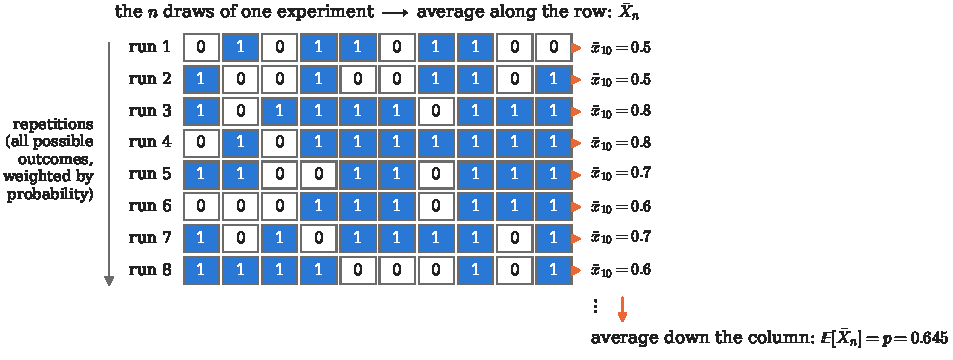
\includegraphics[width=\textwidth]{fig_two_averages}
\caption{Two kinds of averaging. Each row is one run of the experiment, here $n = 10$ Bernoulli draws with $p = 0.645$; averaging along the row gives that run's sample mean, a different number each time. The expectation averages down the column, over every possible run weighted by its probability (only eight runs are shown; the expectation uses all $2^{10}$ of them). The first average is a random variable; the second is the number $p$.}
\label{fig:twoaverages}
\end{figure}

Now, consider the variance of $\bar{X}_n$:
\[
\var(\bar{X}_n) = \frac{\var(X_1 + \cdots + X_n)}{n^2} = \frac{n \sigma^2}{n^2} = \frac{\sigma^2}{n}.
\]

This follows since the $X_i$'s are independent so that the variance of the sum is the sum of the individual variances.

\begin{intuition}[why the variance of the sample mean is scaled by $1/n$]
Averaging $n$ independent draws cancels noise.
Think of each $X_i$ as $\mu + U_i$ where the $U_i$ are independent, mean-zero errors.
Then $\bar{X}_n = \mu + \bar{U}_n$, and the errors in $\bar{U}_n$ have no reason to line up: some are positive, some negative, and summing $n$ of them produces a total whose typical size grows like $\sqrt{n}$, not like $n$ (variances add, so standard deviations add in quadrature).
Dividing by $n$ then leaves a typical error of size $\sigma \sqrt{n}/n = \sigma/\sqrt{n}$.
That's why $\var(\bar{X}_n) = \sigma^2/n$ and why doubling the precision costs four times the data.
\Cref{fig:whyrootn} is that claim drawn: the sum of $n$ cancelling errors reaches about $\sqrt{n}$, not $n$.
\end{intuition}

\begin{figure}[htbp]
\centering
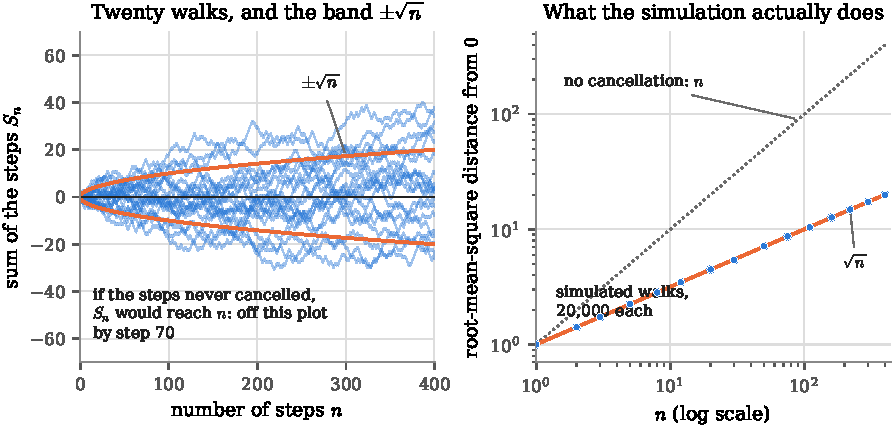
\includegraphics[width=\textwidth]{fig_why_root_n}
\caption{Where the $\sqrt{n}$ in every formula in this book comes from. Left: twenty running sums of steps of $+1$ and $-1$, each step equally likely, with the band $\pm\sqrt{n}$ drawn over them. If the steps never cancelled, the sum after $n$ steps would be $n$, which leaves the top of this figure by step $70$. Because they cancel, the sum stays inside a band that widens like $\sqrt{n}$. Right: the root-mean-square distance of the sum from zero, measured over $20{,}000$ simulated runs at each $n$, against $\sqrt{n}$ and against $n$ on logarithmic axes. The simulated points sit on $\sqrt{n}$, which is exact here: $\E[S_n^2] = n$, since each step has variance $1$ and the cross terms have expectation zero.}
\label{fig:whyrootn}
\end{figure}

\begin{sanitycheck}[The cost of precision]
Any time you produce a standard error, ask what it would take to halve it.
The answer is always four times the data, and it follows from the $\sqrt{n}$: to replace $\sigma/\sqrt{n}$ by $\sigma/(2\sqrt{n})$ you need $\sqrt{n}$ to double, so $n$ must quadruple.
If a calculation of yours implies that twice the data halves the error, you have divided by $n$ somewhere that should have been $\sqrt{n}$.
For the kiss experiment, the standard error at $n = 124$ is $0.043$; getting it to $0.02$ takes not $250$ couples but about $570$.
\end{sanitycheck}

Now, Chebyshev's inequality says that the probability that the distance of some r.v.\ from its mean is larger than some number, say $\epsilon$, is bounded above by the variance of the r.v.\ divided by $\epsilon^2$.
In the present context, the variance is $\sigma^2/n$, and so the upper bound is $\ds \frac{\sigma^2}{n \epsilon^2}$.
Formally, this is expressed as:
\[
\Pr(\abs{\bar{X}_n - \mu} \geq \epsilon) \leq \frac{\sigma^2}{n \epsilon^2}.
\]

The WLLN states that if $\epsilon$ is a fixed number and you take the limit of this probability as $n \to \infty$, then the limit converges to 0.
That is, the WLLN states that for any $\epsilon > 0$, as $n \to \infty$ you have:
\[
\Pr(\abs{\bar{X}_n - \mu} \geq \epsilon) = \Pr \left( \abs*{\frac{X_1 + \cdots + X_n}{n} - \mu} \geq \epsilon \right) \to 0.
\]

So the probability of falling far from the mean diminishes to zero as you draw more and more samples.

To make the interpretation of the WLLN more concrete, suppose again that you're conducting one long experiment, and during that experiment you draw $n$ i.i.d.\ r.v.s, $\Xton$, from the same parent distribution.
One way of thinking about the $X_i$ is that each one equals the true mean, $\mu$, plus some measurement noise, $U_i$, where $\E[U_i] = 0$ for all $i$ and the $U_i$ are independent.
You can then express these noisy measurements as $X_i = \mu + U_i$ for $i = 1, \ldots, n$.

So you've got a collection of noisy measurements and then you compute their average.
What the Weak Law of Large Numbers says is that the sample mean, $\bar{X}_n$, is unlikely to be far off from the true mean, $\mu$, of the parent distribution.
And by far off is meant at least $\epsilon$ distance away.
The sample mean is, thus, a good estimator of the true mean.

Here's the proof of the WLLN, which is easily demonstrated with Chebyshev's inequality.

\coreproof{Two lines: Chebyshev's inequality with $\var(\bar{X}_n) = \sigma^2/n$, then $n \to \infty$. This is the proof to know by heart.}
\begin{proof}
\leavevmode % Puts first item on next line
\begin{itemize}

\item Let $\epsilon$ be some positive real number.
Then by Chebyshev's inequality:
\[
\Pr(\abs{\bar{X}_n - \mu} \geq \epsilon) \leq \frac{\var(\bar{X}_n)}{\epsilon^2} = \frac{\sigma^2}{n \epsilon^2}.
\]

\item As $n \to \infty$, the right-hand side goes to 0, which implies $\Pr(\abs{\bar{X}_n - \mu} \geq \epsilon)$ goes to 0, too.
\end{itemize}
\end{proof}

\begin{worked}[the kiss experiment and Chebyshev]
In the kiss experiment $R_i \iid \Bern(p)$, so $\mu = p$ and $\sigma^2 = p(1-p)$.
How likely is it that the sample proportion misses $p$ by more than $0.084$ (about $10$ couples out of $124$)?
Chebyshev's inequality with $n = 124$, $\epsilon = 0.084$ and the worst case $p(1-p) \leq 1/4$ gives
\[
\Pr(\abs{\bar{R}_n - p} \geq 0.084) \leq \frac{p(1-p)}{n \epsilon^2} \leq \frac{0.25}{124 \times 0.084^2} \approx 0.29,
\]
and with $p(1-p)$ evaluated at $0.645$ the bound is $0.26$.
The bound is true but loose: the CLT (\cref{ch:clt}) says the probability is really about $0.05$.
Chebyshev's inequality is the right tool for proving that something converges, and the wrong tool for saying how fast.
\Cref{fig:bounds} in the next chapter shows all the bounds on the same axes.
\end{worked}

\begin{bridge}[consistency]
An estimator that converges in probability to the parameter it estimates is called \textit{consistent}.
The WLLN says the sample mean is a consistent estimator of the population mean, and the sample proportion is a consistent estimator of the population proportion.
In an introductory course you were told `with a bigger sample the estimate gets closer to the truth'; the WLLN is that sentence with every word defined.
Note what it does not say: it doesn't say $\bar{X}_n$ equals $\mu$ for any finite $n$, and it doesn't say how big $n$ must be for a given accuracy.
The CLT and Hoeffding's inequality, both in \cref{ch:clt}, handle the second question.
\end{bridge}

\section{What comes next}
\label{sec:lln-next}

The Law of Large Numbers says where $\bar{X}_n$ ends up: at $\mu$, with the variance $\sigma^2/n$ shrinking to nothing.
That's the left panel of \cref{fig:twoviews}, and it leaves the obvious question open.
If every density in that panel is on its way to becoming a spike, what does $\bar{X}_n$ look like \textit{along the way}?
The right panel already gave the answer in a picture: magnify the error by $\sqrt{n}$ and its shape settles down to a Gaussian, whatever the parent distribution.
Making that picture into a theorem needs the second mode of convergence, and it's the subject of the next chapter.

\section{Summary}
\label{sec:lln-summary}

\begin{itemize}[nosep]
\item A sequence of r.v.s is a sequence of functions on the sample space; one outcome fixes one ordinary sequence of numbers. No single index $N$ works for every outcome, so convergence has to be defined through probabilities.
\item `Asymptotic' means: for the $n$ at hand, replace the unknown sampling distribution by its limit, usually a Gaussian, and carry on; the theorem does not say how large $n$ must be.
\item $\bar{X}_n$ is a random variable, the theoretical sample mean; $\bar{x}_n$ is the number one sample produced. Every theorem is about the first. Its expectation is a second average, over all possible samples, of the first.
\item \textbf{Convergence in probability:} $X_n \convp X$ if $\Pr(\abs{X_n - X} \geq \epsilon) \to 0$ for every $\epsilon > 0$. The mass outside any band around the limit disappears.
\item \textbf{Shrinking-variance criterion:} $\E[T_n] \to \mu$ and $\var(T_n) \to 0$ imply $T_n \convp \mu$. This is Chebyshev's inequality, and it's how consistency is usually proved.
\item \textbf{Weak Law of Large Numbers:} $\bar{X}_n \convp \mu$ whenever the variance is finite because $\E[\bar{X}_n] = \mu$ and $\var(\bar{X}_n) = \sigma^2/n$. Estimators built from averages are consistent.
\item Chebyshev's bound $\sigma^2/(n\epsilon^2)$ is a guarantee at every $n$ but a loose one: $0.26$ in the kiss experiment where the truth is $0.05$.
\end{itemize}

\section{Exercises}
\label{sec:lln-exercises}

\begin{exercise}
Let $X_n \sim \Bern(1/n)$. (a) For $0 < \epsilon < 1$, what is $\Pr(\abs{X_n} > \epsilon)$? (b) Does $(X_n)$ converge in probability, and to what? (c) Does it converge in distribution? (d) What is $\lim_n \E[\cos(X_n)]$?
\end{exercise}
\begin{solution}
(a) $\Pr(\abs{X_n} > \epsilon) = \Pr(X_n = 1) = 1/n$. (b) Yes, to $0$, since $1/n \to 0$. (c) Yes, to $0$: convergence in probability implies convergence in distribution (\cref{prop:convp-implies-convd} in the next chapter), or directly, the CDF of $X_n$ is $1 - 1/n$ on $[0, 1)$ and $1$ from $1$ on, which converges to the CDF of the constant $0$ at every $x$ (at $x = 0$ too, here). (d) $\E[\cos X_n] = (1 - \frac1n)\cos 0 + \frac1n \cos 1 \to 1$; the next chapter's \cref{prop:convd-equiv} says this is no accident, since $\cos$ is continuous and bounded.
\end{solution}

\begin{exercise}
Let $\Xton \iid \Expo(\lambda)$, so $\E[X_1] = 1/\lambda$ and $\var(X_1) = 1/\lambda^2$. Use the shrinking-variance criterion to show that $\bar{X}_n \convp 1/\lambda$, and find the smallest $n$ for which Chebyshev's inequality guarantees $\Pr(\abs{\bar{X}_n - 1/\lambda} \geq 0.1/\lambda) \leq 0.05$.
\end{exercise}
\begin{solution}
$\E[\bar{X}_n] = 1/\lambda$ for every $n$ and $\var(\bar{X}_n) = 1/(n\lambda^2) \to 0$, so \cref{prop:shrinking-variance} applies. Chebyshev with $\epsilon = 0.1/\lambda$ gives $\Pr(\abs{\bar{X}_n - 1/\lambda} \geq 0.1/\lambda) \leq \frac{1/(n\lambda^2)}{0.01/\lambda^2} = \frac{100}{n}$, which is at most $0.05$ once $n \geq 2000$. The CLT of the next chapter, used as in its exercise 4, gives $n \approx 1.96^2/0.01 \approx 385$, which is the usual gap between a bound and the truth.
\end{solution}

\begin{exercise}
In the kiss model with $p = 0.645$, how many couples would Chebyshev's inequality require before $\Pr(\abs{\bar{R}_n - p} \geq 0.02) \leq 0.05$? Is the answer sensitive to $p$?
\end{exercise}
\begin{solution}
$\Pr(\abs{\bar{R}_n - p} \geq 0.02) \leq p(1-p)/(n \times 0.0004) \leq 0.05$ requires $n \geq p(1-p)/(0.00002) = 0.229/0.00002 \approx 11{,}450$. With the worst case $p(1-p) = 1/4$ the requirement is $12{,}500$; the dependence on $p$ is mild because $p(1-p)$ is flat near $1/2$.
\end{solution}

\chapter{The Central Limit Theorem}
\label{ch:clt}

\begin{chaptergoals}
\begin{itemize}[nosep]
\item Convergence in distribution, the mode of convergence that compares CDFs rather than values, and why its definition only looks at continuity points.
\item The Central Limit Theorem in its three equivalent forms, and what it says at the sample sizes you actually have.
\item Hoeffding's inequality: a finite-sample guarantee for bounded data when $n$ is too small to trust the CLT.
\item What the limit theorems buy you, and which of their conclusions could be reached without limits.
\end{itemize}
\Cref{ch:lln} ended with $\bar{X}_n$ collapsing onto $\mu$ and the question of what it looks like on the way there. This chapter answers it.
\end{chaptergoals}

\section{Convergence in distribution}
\label{sec:conv-dist}

Convergence in distribution is weaker than convergence in probability (and, in the full hierarchy of \cref{app:modes}, the weakest mode there is).
All it says is that the CDF of $X_n$ converges to the CDF of $X$ as $n$ goes to infinity, \textit{but doesn't require any dependence between the} $X_n$'\textit{s} \textit{and} $X$.
That is, the r.v.s $X_n$ and $X$ can be defined on entirely different probability spaces.
The CDF of these r.v.s is used instead of a PDF or PMF because all r.v.s, whether they be discrete, continuous or mixed, have CDFs.

\textbf{Question:} Why does not requiring any dependence between the $X_n$'s and $X$ make convergence in distribution weak?
You might think that, by not introducing a dependence assumption, you're actually making the statement stronger.

\textbf{Answer:} By not imposing any dependence structure between $X_n$ and $X$, convergence in distribution allows for a wider range of scenarios where the CDFs of $X_n$ converge to the CDF of $X$.
It doesn't guarantee that the actual values of $X_n$ get closer to $X$ as $n$ increases, which is a requirement for stronger forms of convergence like convergence in probability or convergence almost surely.
Convergence in distribution only concerns the limiting behavior of the distributions, not the actual values of the r.v.s.
A statement that holds in more scenarios is a weaker statement because it tells you less about any one of them.

\begin{definition}[Convergence in distribution]
\label{def:convd}
A sequence $(X_n)_{n \geq 1}$ of r.v.s \textbf{converges in distribution} to an r.v.\ $X$, denoted $X_n \convd X$, if:
\[
\lim_{n \to \infty} F_{X_n}(x) = F_X(x),
\]
for all $x$ at which $F_X$ is continuous.
\end{definition}

\begin{inwords}
\textbf{In words.} For each fixed $x$, $F_{X_n}(x) = \Pr(X_n \leq x)$ is a number, and the definition asks that this sequence of numbers converge to $\Pr(X \leq x)$, at every $x$ where the limit's CDF has no jump \toolkit{sec:math-density}. It compares two distributions, not two random variables: nothing is said about $X_n$ and $X$ being close on any outcome, and they need not even live on the same sample space.
\par\smallskip
\textbf{For the kiss data.} The CLT will say that the standardized error $\sqrt{n}(\bar{R}_n - p)/\sqrt{p(1-p)}$ converges in distribution to $\Gauss(0,1)$: for every $x$, the probability that the standardized error is below $x$ approaches $\Phi(x)$. With $n = 124$ that is the license to compute $\Pr(\abs{\bar{R}_n - p} \leq 0.084) \approx \Phi(1.95) - \Phi(-1.95) = 0.95$.
\end{inwords}

\subsection{Why only the continuity points?}

The qualifier `at which $F_X$ is continuous' looks like a technicality.
It isn't; without it the most basic examples fail.

\begin{example}
\label{ex:unif-shrinking}
Let $T_n \sim \text{Unif}\left(\left[5 - \frac{1}{2n}, 5 + \frac{1}{2n}\right]\right)$, a uniform on an interval of width $1/n$ centered at $5$.
Every sensible notion of convergence should say $T_n \to 5$, and indeed $T_n \convp 5$ since $\Pr(\abs{T_n - 5} > \delta) = 0$ as soon as $\frac{1}{2n} \leq \delta$.
The CDF $F_n$ of $T_n$ is $0$ to the left of the interval, rises linearly to $1$ across it, and in particular $F_n(5) = \frac12$ for \textit{every} $n$.
The CDF of the constant $5$ is the step function $F(t) = \ind(t \geq 5)$, with $F(5) = 1$.
So $F_n(t) \to F(t)$ for every $t \neq 5$ but not at $t = 5$, the one point where $F$ jumps.
With the continuity-point qualifier, $T_n \convd 5$; without it, $T_n$ wouldn't converge in distribution to anything.
\Cref{fig:cdfcont} shows the picture: the $F_n$ close in on the step function everywhere except at the jump, where all of them pass through $\frac12$, and the definition of convergence in distribution excludes exactly that point.
\end{example}

\begin{figure}[htbp]
\centering
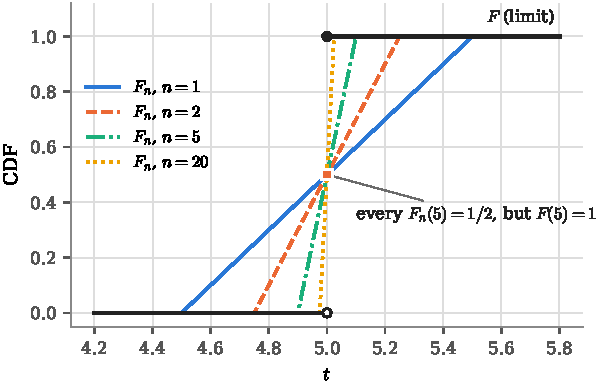
\includegraphics[width=0.7\textwidth]{fig_cdf_continuity_points}
\caption{The CDFs $F_n$ of $T_n \sim \text{Unif}([5 - \frac{1}{2n}, 5 + \frac{1}{2n}])$ for $n = 1, 2, 5, 20$, and the CDF $F$ of the constant $5$ in black. The orange square marks the point $(5, \frac12)$ that every $F_n$ passes through.}
\label{fig:cdfcont}
\end{figure}

The general principle: a jump in $F_X$ at $x$ means $X$ has positive probability of equaling $x$ exactly, and a sequence approaching from the left or the right can straddle that jump forever.
Away from the jumps there's nothing to straddle.

\subsection{Two equivalent definitions}

Alternatively, convergence in distribution can be defined using the expectation of a function, provided the function is continuous and bounded.
This is the form that generalizes: on spaces where there is no CDF to write down, it becomes the definition of convergence in distribution.

\begin{proposition}[Equivalent characterizations]
\label{prop:convd-equiv}
For real-valued r.v.s the following are equivalent:
\begin{enumerate}[nosep]
\item $F_{X_n}(x) \to F_X(x)$ for all $x$ at which $F_X$ is continuous;
\item $\E[f(X_n)] \to \E[f(X)]$ for every continuous and bounded function $f: \real \to \real$.
\end{enumerate}
If moreover $X$ has a density (for instance $X$ is Gaussian), then $X_n \convd X$ implies convergence of interval probabilities:
\[
\Pr(a \leq X_n \leq b) \to \Pr(a \leq X \leq b), \qquad \text{for all } a < b.
\]
\end{proposition}

Note that in (2) the things converging are numbers, $\E[f(X_n)]$, so the convergence is ordinary convergence of numbers.
The second form is the useful one in proofs because it doesn't single out any particular $x$; the first form is the useful one in computations because CDFs are what you can write down.
The last statement is why the CLT is enough to compute probabilities: $\Pr(a \leq Z_n \leq b) \approx \Phi(b) - \Phi(a)$, which is what every asymptotic confidence interval and test rests on.

One implication between the two modes is used on nearly every page from here on, so here it is as a statement with a proof.

\begin{proposition}[In probability implies in distribution]
\label{prop:convp-implies-convd}
If $X_n \convp X$, then $X_n \convd X$.
\end{proposition}

\optionalproof{Sandwich $F_{X_n}(x)$ between $F_X(x - \epsilon)$ and $F_X(x + \epsilon)$, up to the probability that $X_n$ and $X$ differ by more than $\epsilon$, which goes to $0$; then let $\epsilon \to 0$ and use continuity of $F_X$ at $x$. The statement is what matters; the proof is a standard $\epsilon$ argument.}
\begin{proof}
Fix a continuity point $x$ of $F_X$ and an $\epsilon > 0$.
If $X_n \leq x$ then either $X \leq x + \epsilon$ or $\abs{X_n - X} > \epsilon$, so
\[
F_{X_n}(x) \leq F_X(x + \epsilon) + \Pr(\abs{X_n - X} > \epsilon).
\]
In the same way, if $X \leq x - \epsilon$ then either $X_n \leq x$ or $\abs{X_n - X} > \epsilon$, so
\[
F_X(x - \epsilon) - \Pr(\abs{X_n - X} > \epsilon) \leq F_{X_n}(x).
\]
Let $n \to \infty$: the probability terms vanish by convergence in probability, and $F_{X_n}(x)$ is squeezed, in the limit, between $F_X(x - \epsilon)$ and $F_X(x + \epsilon)$.
Now let $\epsilon \to 0$: both bounds tend to $F_X(x)$ because $F_X$ is continuous at $x$.
\end{proof}

The continuity-point qualifier is what the last line uses: at a jump of $F_X$ the two bounds would not meet, and \cref{ex:unif-shrinking} shows the conclusion can indeed fail there.

\begin{example}
\label{ex:cos}
In \cref{ex:bern-1-over-n}, $X_n \sim \Bern(1/n)$ converges in probability, hence in distribution, to $0$.
The function $f(x) = \cos x$ is continuous and bounded, so $\E[\cos(X_n)] \to \cos(0) = 1$.
You can check this directly: $\E[\cos X_n] = (1 - \frac1n) \cos 0 + \frac1n \cos 1 \to 1$.
\end{example}

\subsection{Example 1: i.i.d.\ random variables}

If $(X_n)_{n \geq 1}$ is a sequence of i.i.d.\ r.v.s, then convergence in distribution isn't very interesting because they converge to the CDF of any one r.v.\ in the sequence.
That is, if $X_1, X_2, \ldots$ is a sequence of i.i.d.\ r.v.s with CDF $F_X(x)$, then $X_n \convd X$.
This is because:
\[
F_{X_n}(x) = F_X(x), \text{ for all } x \, \text{ implies that } \lim_{n\to \infty} F_{X_n}(x) = F_X(x), \, \text{ for all } x.
\]

This is the example from \cref{sec:conv-why}: the sequence of standard Gaussians converges in distribution to a standard Gaussian even though $\Pr(X_n = X) = 0$.
Convergence in distribution is the mode that makes sense of that example.

\subsection{Example 2: the maximum of uniforms}

\begin{example}
\label{ex:max-unif}
Let $X_1, X_2, \ldots \iid \text{Unif}([0,1])$ and define the maximum of the first $n$ by $\ds X_{(n)} = \max_{i=1,\ldots,n} X_i$.
Then:
\[
n(1 - X_{(n)}) \convd \Expo(1).
\]
\end{example}

Before the proof, a word on why the maximum is being magnified by $n$ rather than $\sqrt{n}$.
The maximum of $n$ uniforms piles up just below $1$; by the same argument as in \cref{ex:min-unif} it converges in probability to $1$, so the unmagnified sequence has a degenerate limit.
The gap $1 - X_{(n)}$ is of order $1/n$ (with $n$ points spread over $[0,1]$ the largest one sits about $1/n$ from the top), so $n$ is the magnification that holds its size fixed.
The CLT's $\sqrt{n}$ is for sums; a maximum is not a sum and gets a different rate and a different (non-Gaussian) limit.

\coreproof{Write the CDF of $n(1 - X_{(n)})$ as a probability about the whole sample, use independence to get a power $(1 - x/n)^n$, and recognize the limit $e^{-x}$ \toolkit{sec:math-explog}. Same template as \cref{ex:min-unif}, with a CDF in place of a tail probability.}
\begin{proof}
\leavevmode % Puts first item on next line
\begin{itemize}

\item Define the CDF of the r.v.\ $n(1 - X_{(n)})$ at a point $x > 0$:
\[
F_{n(1 - X_{(n)})} (x) = \Pr(n(1 - X_{(n)}) \leq x).
\]

\item Now, simplify the CDF in such a way as to eventually take the limit as $n \to \infty$.

\item To that end, observe that:
\begin{align*}
\Pr(n(1 - X_{(n)}) \leq x) &= \Pr(n - nX_{(n)} \leq x ) \\
								&= \Pr \left(X_{(n)} \geq 1 - \frac{x}{n} \right) \\
								&= 1 - \Pr \left(X_{(n)} < 1 - \frac{x}{n} \right) \\
								&= 1 - \Pr \left( X_1 < 1 - \frac{x}{n}, X_2 < 1 - \frac{x}{n}, \ldots, X_n < 1 - \frac{x}{n} \right)  \\
								&= 1 - \Pr \left(X_1 < 1 - \frac{x}{n} \right)  \Pr \left( X_2 < 1 - \frac{x}{n} \right)  \cdots \Pr \left( X_n < 1 - \frac{x}{n} \right)  \\
								&= 1 - \Pr \left( X_1 < 1 - \frac{x}{n}\right)^n.
\end{align*}

The movement from the third to the fourth equality holds because, as $X_{(n)}$ is the maximum of the $X_i$'s, the maximum is below a level exactly when every $X_i$ is below it: the single event is equivalent to the joint event.
The fifth equality results since the $X_i$'s are independent.

\item Now, recall that the $X_i$'s, and thus $X_1$, are uniformly distributed on $(0,1)$.
This means its CDF is linear, emanating from the origin rising to 1 with a slope of 1;
in other words, plug any value of the support into the CDF and you get the same value back.
Hence, for $n$ large enough that $1 - x/n \in (0,1)$:
\[
\Pr \left( X_1 < 1 - \frac{x}{n}\right) = 1 - \frac{x}{n}.
\]

\item Returning to the last right-hand side from above, you have that:
\[
1 - \Pr \left( X_1 < 1 - \frac{x}{n}\right)^n = 1 -  \left( 1 - \frac{x}{n} \right)^n,
\]

which by taking the limit as $n \to \infty$ gives:
\[
\lim_{n \to \infty} \left[ 1 -  \left( 1 - \frac{x}{n} \right)^n \right] = 1 - e^{-x},
\]

using the calculus fact $(1 - x/n)^n \to e^{-x}$.

\item To summarize, then, you have:
\[
\lim_{n \to \infty} \Pr(n(1 - X_{(n)}) \leq x) = 1 - e^{-x} \quad \text{for every } x > 0,
\]

and $1 - e^{-x}$ is the CDF of the Exponential with $\lambda = 1$ (for $x \leq 0$ both sides are $0$).
This proves the result.
\end{itemize}
\end{proof}

\Cref{fig:maxunif} shows the result by simulation.
On the left, the maximum of $n = 50$ uniforms crowds the top of the interval.
On the right, the magnified gap $n(1 - X_{(n)})$ is already very close to $\Expo(1)$ at $n = 50$.

\begin{figure}[htbp]
\centering
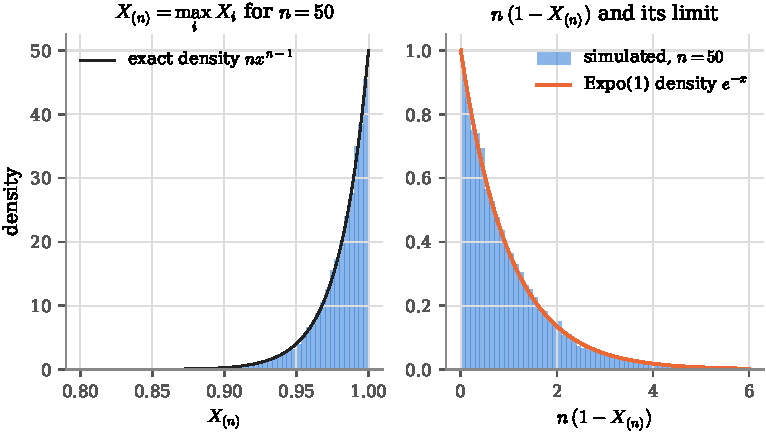
\includegraphics[width=\textwidth]{fig_max_uniform_expo}
\caption{\Cref{ex:max-unif} by simulation, $20{,}000$ replications at $n = 50$. Left: histogram of the maximum $X_{(n)}$ of $n$ uniforms, with its exact density $n x^{n-1}$ in black. Right: histogram of $n(1 - X_{(n)})$, with the $\Expo(1)$ density in orange.}
\label{fig:maxunif}
\end{figure}

\begin{pitfall}[convergence in distribution says nothing about closeness]
Let $Z \sim \Gauss(0,1)$ and set $X_n = -Z$ for every $n$.
By the symmetry of the Gaussian, $X_n \sim \Gauss(0,1)$ for every $n$, so $X_n \convd Z$.
But $\abs{X_n - Z} = 2\abs{Z}$, which is not small and never becomes small.
So $X_n$ does not converge in probability to $Z$, even though it converges in distribution to it.
Convergence in distribution is a statement about two CDFs, not about two columns of numbers getting closer.
The same example shows why you can't add limits in distribution: $X_n + Z = 0$ for every $n$, while the sum of two independent $\Gauss(0,1)$ r.v.s is $\Gauss(0,2)$.
Knowing the limiting distributions of $X_n$ and $Y_n$ separately doesn't determine the limiting distribution of $X_n + Y_n$; you need to know how they're related.
\Cref{ch:limit-tools} says what you can do instead.
\end{pitfall}


\subsection{Limits that are constants}

One case of convergence in distribution is used constantly later, so here it is as a statement with a proof.

\begin{proposition}
\label{prop:convd-constant}
If $X_n \convd c$ for a constant $c$, then $X_n \convp c$.
\end{proposition}

\optionalproof{The CDF of a constant is a step; convergence of the CDFs at two continuity points, one on each side of $c$, squeezes the mass outside the $\epsilon$-band to $0$.}
\begin{proof}
The CDF of the constant $c$ is the step $F(x) = \ind(x \geq c)$, continuous everywhere except at $c$.
Fix $\epsilon > 0$.
The points $c - \epsilon$ and $c + \epsilon/2$ are continuity points, so $F_{X_n}(c - \epsilon) \to F(c - \epsilon) = 0$ and $F_{X_n}(c + \epsilon/2) \to F(c + \epsilon/2) = 1$.
Therefore
\[
\Pr(\abs{X_n - c} \geq \epsilon) = \Pr(X_n \leq c - \epsilon) + \Pr(X_n \geq c + \epsilon) \leq F_{X_n}(c - \epsilon) + \left( 1 - F_{X_n}(c + \epsilon/2) \right) \to 0 + 0. \qedhere
\]
\end{proof}

For a constant limit, then, `in probability' and `in distribution' are the same thing, which is why the Law of Large Numbers could equally be written with the arrow for convergence in distribution, and why Slutsky's theorem in \cref{ch:limit-tools} needs only convergence in probability for the sequence with the constant limit.

\section{The Central Limit Theorem}
\label{sec:clt}

As in the previous section, let $X_1, X_2, \ldots$ be i.i.d.\ r.v.s with mean $\mu$ and variance $\sigma^2$.
The Law of Large Numbers says that as $n \to \infty$, $\bar{X}_n$ converges to the constant $\mu$.
But what is $\bar{X}_n$'s distribution along the way to becoming the constant $\mu$?
This is addressed by the Central Limit Theorem (CLT), an all-important theorem in statistics.

The CLT states that for large $n$, the distribution of $\bar{X}_n$ \textit{after standardization} approaches a standard Gaussian distribution.
Recall that if you standardize an r.v., the resulting r.v.\ is measured in units of standard deviation.
In the present case, the convergence process examines the typical deviations of $\bar{X}_n$ around $\mu$.
Now the statement of the CLT.

\begin{theorem}[Central Limit Theorem]
\label{thm:clt}
Let $\Xton$ be i.i.d.\ r.v.s such that $\E[X_i] = \mu$ and $\var(X_i) = \sigma^2 < \infty$ for $i = 1, \ldots, n$.
Then:
\[
\sqrt{n} \left( \frac{\bar{X}_n - \mu}{\sigma} \right) \convd \Gauss(0, 1).
\]
In words, the CDF of the left-hand side converges to $\Phi$, the CDF of the standard Gaussian distribution.
\end{theorem}

An equivalent statement of the CLT in which $\bar{X}_n$ remains mean-centered by $\mu$ but omits the standardization by $\sigma$ is given as follows:
\[
\sqrt{n} \left( \bar{X}_n - \mu \right) \convd \Gauss(0, \sigma^2).
\]

\textbf{Question 1:} Why does this second statement hold?

\textbf{Answer 1:} It holds because of the way the Gaussian family behaves under scaling.
Let $X \sim \Gauss(0, 1)$, so its PDF is:
\[
f_X(x) = \frac{1}{\sqrt{2 \pi} } \exp \left( - \frac{x^2}{2} \right).
\]

Now let $Y = \sigma X$ for some $\sigma > 0$.
Then $\E[Y] = \E[\sigma X] = \sigma \E[X] = 0$.
Hence the mean remains 0.
But note what happens to the variance of $X$ after multiplying it by $\sigma$:
\begin{align*}
\var(Y) = \E[(Y - \E[Y])^2] &= \E[(\sigma X - 0)^2] \\
	&= \sigma^2 \E[X^2] \\
	&= \sigma^2 \var(X) \\
	&= \sigma^2,
\end{align*}

and $Y$ is still Gaussian (a linear function of a Gaussian is Gaussian), so $\sigma X \sim \Gauss(0, \sigma^2)$.
Multiplying both sides of the first statement by the constant $\sigma$ therefore gives the second; the step `multiply both sides of a limit in distribution by a constant' is justified by the continuous mapping theorem of \cref{ch:limit-tools}.

\textbf{Question 2:} In the statement of the CLT the r.v.\ $\ds \sqrt{n} \left( \frac{\bar{X}_n - \mu}{\sigma} \right)$ converges to the standard Gaussian distribution.
The term in parentheses standardizes $\bar{X}_n$;
that is, the mean, $\mu$, is subtracted from $\bar{X}_n$, and the result divided by the standard deviation, $\sigma$.
But why multiply this standardized term by $\sqrt{n}$?

\textbf{Answer 2:} Because $\sigma$ is the standard deviation of a single $X_i$, not of $\bar{X}_n$.
The standard deviation of the sample mean equals $\sigma/\sqrt{n}$.\footnote{To see why, let $\Xton$ be i.i.d.\ r.v.s.
By independence, you have that:
\[
\var(\bar{X}_n) = \var\left( \frac{X_1}{n} + \cdots + \frac{X_n}{n} \right) = \frac{\sigma^2}{n^2} + \cdots + \frac{\sigma^2}{n^2} = \frac{n \sigma^2}{n^2} = \frac{\sigma^2}{n}.
\]}
Standardizing $\bar{X}_n$ properly means dividing by \textit{its} standard deviation, and division by a fraction is multiplication by its reciprocal:
\[
\frac{\bar{X}_n - \mu}{\sigma/\sqrt{n}} = \sqrt{n} \left( \frac{\bar{X}_n - \mu}{\sigma} \right).
\]
So the $\sqrt{n}$ isn't an extra factor; it's the part of the standardization that's easy to lose track of.

A third and equivalent statement of the CLT uses a standardized sum.
Define the standardized sum of $X_1 + \cdots + X_n$ by:
\[
Z_n = \frac{n \bar{X}_n - n \mu}{\sqrt{n} \sigma},
\]

where $n \bar{X}_n$ is just $X_1 + \cdots + X_n$.
As $Z_n$ is standardized it follows that $\E(Z_n) = 0$ and $\var(Z_n) = 1$.
Further, let $Z$ be a standard Gaussian r.v.
Then the CLT states that:
\[
\lim_{n \to \infty} \Pr(Z_n \leq z) = \Pr(Z \leq z), \text{ for every } z,
\]

where $\Pr(Z \leq z)$ is the standard Gaussian CDF $\Phi(z)$.
The reason why the CLT states that the CDF of $Z_n$ (and not its PDF) converges to the standard Gaussian CDF is because the result applies to \textit{all} r.v.s with finite variance, and all r.v.s have CDFs.
The $X_i$ can be discrete, as in the kiss experiment, in which case $Z_n$ has no PDF at all.

\textbf{Question 3:} Why do you standardize the sums of the $X_i$'s for the approximation?

\textbf{Answer 3:} Suppose the $X_1 + \cdots + X_n$ aren't standardized.
Then $\E(X_1 + \cdots + X_n) = n \mu$ and $\var(X_1 + \cdots + X_n) = n \sigma^2$.
Both are finite for every $n$, but neither stays bounded as $n \to \infty$: the unstandardized sum drifts off (its mean is $n\mu$) and spreads out (its standard deviation is $\sigma\sqrt{n}$), so no fixed distribution can describe it and its CDF has no limit that is a CDF.
Standardizing pins the sum down, with $\E(Z_n) = 0$ and $\var(Z_n) = 1$ for all $n$, so that a limiting distribution has a chance to exist.

\begin{figure}[htbp]
\centering
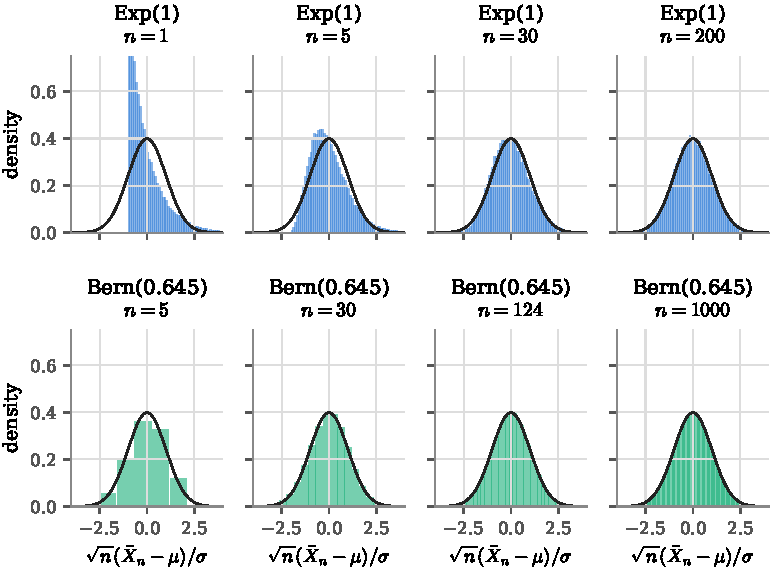
\includegraphics[width=\textwidth]{fig_clt_in_action}
\caption{The standardized sample mean $\sqrt{n}(\bar{X}_n - \mu)/\sigma$, with the $\Gauss(0,1)$ density in black over it. Top row: $\Expo(1)$ draws at $n = 1, 5, 30, 200$, histograms from $50{,}000$ simulated samples. Bottom row: $\Bern(0.645)$ draws at $n = 5, 30, 124, 1000$, the exact Binomial distribution as bars.}
\label{fig:cltaction}
\end{figure}

\begin{bridge}[the `$n \geq 30$' rule]
Introductory courses offer a rule of thumb: the normal approximation to the sample mean is fine once $n \geq 30$.
The CLT contains no such number.
It's a limit statement, and how fast the limit is reached depends on the parent distribution: above all on how asymmetric and heavy-tailed it is.
In the top row of \cref{fig:cltaction} the parent is the strongly skewed $\Expo(1)$, and the skew is still visible at $n = 30$.
In the bottom row the parent is the kiss experiment's $\Bern(0.645)$; the standardized mean lives on a lattice, visible as bars, and by $n = 124$ the Gaussian is already an excellent description.
For a symmetric parent, $n = 5$ can be enough; for a heavily skewed one, $n = 200$ may not be.
What is a theorem is the \textit{rate}: the Berry--Esseen bound says the gap between the CDF of $Z_n$ and $\Phi$ is at most a universal constant times $\E\abs{X - \mu}^3 / (\sigma^3 \sqrt{n})$, so the error shrinks like $1/\sqrt{n}$, slowly when the ratio $\E\abs{X - \mu}^3/\sigma^3$ is large, as it is for skewed and heavy-tailed parents.
A finer expansion (the Edgeworth expansion) shows that, for a continuous parent, the leading term of the error is proportional to the parent's skewness, which is why symmetric parents reach the Gaussian faster in practice.
\end{bridge}

\subsection{The essence of the CLT: a `stochastic' bound}

Due to the so-called `empirical rule', values between $-3$ and $3$ in the support of a standard Gaussian account for nearly 100\% of its probability mass ($99.7\%$ of it).
By the CLT, this implies that, for $n$ large enough for the approximation to apply, the following inequality holds with probability about $99.7\%$:
\[
\abs{\bar{X}_n - \mu} \leq \frac{3 \sigma}{\sqrt{n}},
\]

since, for every $n$, the two events are the same:
\begin{align*}
\sqrt{n} \left( \frac{\bar{X}_n - \mu}{\sigma} \right) \in [-3, 3] &\Leftrightarrow -3 \leq \sqrt{n} \left( \frac{\bar{X}_n - \mu}{\sigma} \right) \leq 3 \\
&\Leftrightarrow \abs*{ \sqrt{n} \left( \frac{\bar{X}_n - \mu}{\sigma} \right) } \leq 3 \\
&\Leftrightarrow \frac{\sqrt{n}}{\sigma} \abs{ \bar{X}_n - \mu } \leq 3 \\
&\Leftrightarrow \abs{ \bar{X}_n - \mu } \leq  \frac{3 \sigma}{\sqrt{n}}.
\end{align*}

The essence of the CLT is that, despite $\bar{X}_n - \mu$ being an r.v.\ with an unbounded support (when the $X_i$ are unbounded), it's \textit{stochastically} bounded in the sense that, with high probability, it's between $-3\sigma/\sqrt{n}$ and $3\sigma/\sqrt{n}$.
Replace $3$ by $1.96$ and `with high probability' by $95\%$ and you have the recipe for every confidence interval in \cref{ch:confidence-intervals}.
\Cref{fig:funnel} draws the bound as a funnel around the running average, and it is also the chapter's two theorems in one picture.
The funnel narrows like $1/\sqrt{n}$: that is the Law of Large Numbers.
At any fixed $n$ past the first few dozen, about $5\%$ of the paths are outside the inner funnel and almost none outside the outer one (in this simulation, $6\%$ of the points with $n \geq 30$ are outside the inner funnel): that is the stochastic bound.
The inner funnel at $n = 124$ is the width of the confidence interval of \cref{ch:confidence-intervals}.

\begin{bridge}[the `$np \geq 10$ and $n(1 - p) \geq 10$' condition]
An introductory course says the sample proportion is approximately normal, with mean $p$ and standard deviation $\sqrt{p(1-p)/n}$, once $np \geq 10$ and $n(1 - p) \geq 10$ (some books say $5$, some $15$).
That is \cref{thm:clt} for $\Bern(p)$ data, with $\mu = p$ and $\sigma^2 = p(1-p)$; the inner funnel of \cref{fig:funnel} is $p$ plus or minus $1.96$ of those standard deviations.
The condition is stated in counts rather than in $n$ because the Bernoulli parent's skewness, $(1 - 2p)/\sqrt{p(1-p)}$, grows without bound as $p$ nears $0$ or $1$, and the skewness of the count is that divided by $\sqrt{n}$.
With both counts at least $10$ the count's skewness is at most $1/\sqrt{10} = 0.32$ in size, whatever $p$ is; at $p = 0.01$ the condition asks for $n = 1{,}000$, where the `$n \geq 30$' rule would accept $n = 30$ and a skewness of $1.8$.
For the kiss data the counts, with $\hat{p}$ in place of $p$, are the observed $80$ and $44$, and the count's skewness is $-0.05$.
\Cref{sec:tests-kiss} takes up the continuity correction, which repairs the count's discreteness rather than its skewness.
\end{bridge}

\begin{figure}[htbp]
\centering
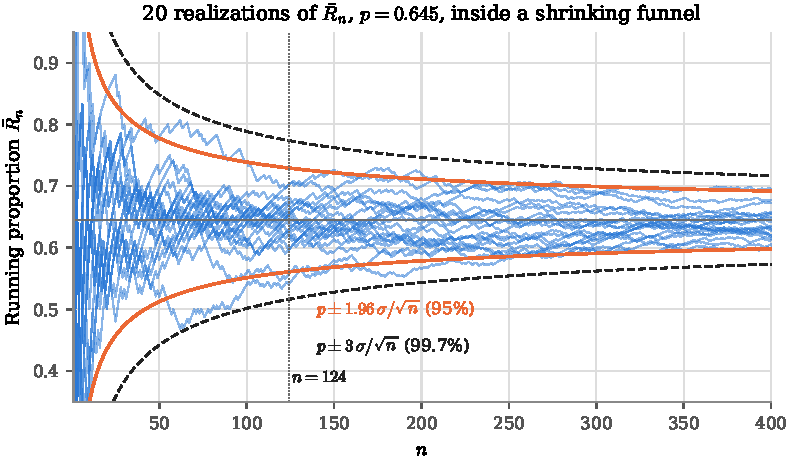
\includegraphics[width=\textwidth]{fig_clt_funnel}
\caption{Twenty realizations of the running proportion $\bar{R}_n$ in the kiss model, $p = 0.645$, with the curves $p \pm 1.96\,\sigma/\sqrt{n}$ (orange) and $p \pm 3\,\sigma/\sqrt{n}$ (dashed black), where $\sigma = \sqrt{p(1-p)}$. The dotted line marks $n = 124$.}
\label{fig:funnel}
\end{figure}

\section{Hoeffding's inequality: help for small sample sizes}
\label{sec:hoeffding}

What if your sample size, $n$, is not large enough to apply the CLT?
Hoeffding's inequality is a helpful tool when $n$ is small that effectively delivers the same essential message as the CLT: $\bar{X}_n$ is close to $\mu$ within some stochastic bound.
The statement isn't as strong as the CLT and requires additional restrictions on the r.v.s.
Namely, the r.v.s must be bounded almost surely, that is, with probability one \toolkit{sec:math-rv}, which rules out any r.v.\ with an arbitrarily large or small support (e.g., Gaussian and Exponential r.v.s).
But despite the stronger restrictions, its power lies in providing a bound on the distance between $\bar{X}_n$ and $\mu$ that is a theorem rather than an approximation, for every $n$, however small.
Here's the statement.

\begin{theorem}[Hoeffding's inequality, 1963]
\label{thm:hoeffding}
Let $n$ be some positive integer and $X, \Xton$ be i.i.d.\ r.v.s such that $\mu = \E[X]$ and $X$ is almost surely bounded within $[a,b]$ where $a < b$.
Then:
\[
\Pr\left( \abs{ \bar{X}_n - \mu } \geq \epsilon \right) \leq 2 \exp \left( - \frac{2n\epsilon^2}{(b-a)^2} \right), \, \, \text{ for all } \epsilon > 0.
\]
\end{theorem}

Compare this with Chebyshev's bound $\sigma^2/(n \epsilon^2)$.
Both go to zero as $n$ grows, but Hoeffding's bound goes to zero \textit{exponentially} fast in $n$ while Chebyshev's goes like $1/n$.
The price is the boundedness assumption, which Chebyshev doesn't need.
Note also what Hoeffding's inequality is not: it's a bound, not an approximation.
The CLT says $\Pr(\abs{\bar{X}_n - \mu} \geq \epsilon) \approx 2(1 - \Phi(\epsilon \sqrt{n}/\sigma))$ for large $n$ without saying how large; Hoeffding says $\Pr(\abs{\bar{X}_n - \mu} \geq \epsilon) \leq 2e^{-2n\epsilon^2/(b-a)^2}$ for every $n \geq 1$, full stop.

\begin{worked}[the kiss experiment, three ways]
The $R_i$ are Bernoulli, so they're bounded in $[0, 1]$ and $(b - a)^2 = 1$.
With $n = 124$ and $\epsilon = 0.084$:
\begin{itemize}[nosep]
\item Chebyshev (with $p(1-p)$ evaluated at $0.645$): $\Pr(\abs{\bar{R}_n - p} \geq 0.084) \leq 0.26$; with the worst case $p(1-p) \leq 1/4$ instead, $0.29$.
\item Hoeffding: $\Pr(\abs{\bar{R}_n - p} \geq 0.084) \leq 2 \exp(-2 \times 124 \times 0.084^2) = 2 e^{-1.75} \approx 0.35$.
\item CLT: $\Pr(\abs{\bar{R}_n - p} \geq 0.084) \approx 2 \left( 1 - \Phi \left( \frac{0.084 \sqrt{124}}{\sqrt{0.645 \times 0.355}} \right) \right) = 2(1 - \Phi(1.95)) \approx 0.05$.
\end{itemize}
At this $n$ the exact Binomial probability is $0.05$, so the CLT approximation is right on and both bounds are loose, with Chebyshev slightly tighter than Hoeffding.
\Cref{fig:bounds} shows that Hoeffding overtakes Chebyshev at about $n = 165$ and is far ahead by $n = 400$, as the exponential must eventually beat $1/n$.
In the figure the CLT approximation sits on top of the exact probability for $n$ beyond a few dozen.
The jaggedness of the exact curve is real: it comes from the lattice of possible values of $\bar{R}_n$ moving relative to the fixed $\epsilon$.
The two bounds are guarantees; the CLT number is an approximation that happens, here, to be excellent.
\end{worked}

\begin{figure}[htbp]
\centering
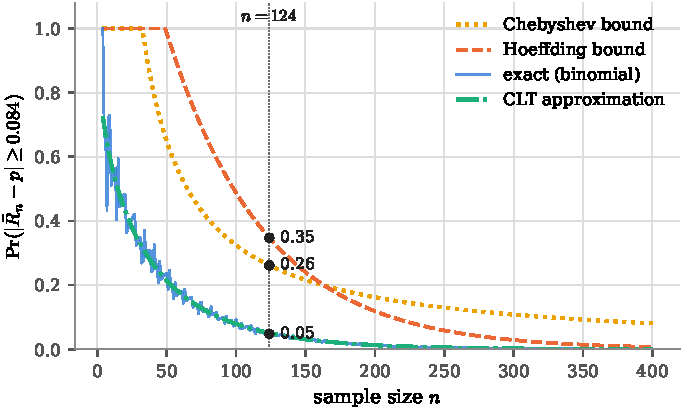
\includegraphics[width=0.85\textwidth]{fig_bounds_vs_truth}
\caption{$\Pr(\abs{\bar{R}_n - p} \geq 0.084)$ in the kiss model with $p = 0.645$, as a function of $n$: the exact Binomial probability, the CLT approximation, and the Chebyshev and Hoeffding upper bounds. The dots mark $n = 124$.}
\label{fig:bounds}
\end{figure}

\section{What the limit theorems buy you}
\label{sec:conv-what-limits-buy}

A fair question at this point: couldn't the results of this chapter and the last be proved without limits?
More of them than you would guess, and it's worth seeing which because it shows what the limit theorems are actually for.

\textbf{Results that have a finite-sample version.}
\begin{itemize}
\item The Law of Large Numbers is Chebyshev's inequality with $n$ sent to infinity.
The finite-$n$ content is the inequality itself, $\Pr(\abs{\bar{X}_n - \mu} \geq \epsilon) \leq \sigma^2/(n\epsilon^2)$; the limit only tidies the statement.
Hoeffding's inequality (\cref{sec:hoeffding}) is the same idea with a better bound; the `conservative' confidence interval of \cref{ch:confidence-intervals} uses the same trick of replacing the unknown variance by its worst case, $p(1-p) \leq 1/4$.
Both are guarantees that hold at $n = 2$ as well as at $n = 10^6$.
\item When the parent distribution is known, an exact sampling distribution replaces the CLT.
For Bernoulli data the sum $n\bar{R}_n$ is Binomial, so the kiss experiment's proportion has exact tests and an exact interval (the Clopper--Pearson interval, which for these data is $[0.55, 0.73]$).
For Exponential data the sum is Gamma, which gives an exact interval for the subway rate $\lambda$ (an exercise in \cref{ch:confidence-intervals}).
For Gaussian data the standardized mean has a $t$ distribution and the ratio of variances an $F$ distribution, which is why the $t$-test of \cref{ch:t-test} and Gaussian linear regression in \cref{ch:regression-multi} need no limit theorem at all.
\item The CLT itself has a finite-sample version: the Berry--Esseen theorem mentioned in \cref{sec:clt} bounds the gap between the CDF of the standardized mean and $\Phi$ at every $n$.
The limit statement is that theorem with the error term dropped.
\end{itemize}

\textbf{What has no finite-sample substitute.}
What you can't do without a limit theorem is get a statement that is both universal and sharp.
Chebyshev and Hoeffding hold for every parent too, but as bounds that may sit far from the truth; an approximation that is accurate for every parent at once is the whole content of the CLT.
It's the only reason the same recipe, estimate $\pm 1.96 \times$ standard error, works for proportions, means, rates, regression coefficients and maximum likelihood estimators of every model in this book.
Without it you must either know the parent exactly, and then compute its exact sampling distribution, which is possible for the three families above and intractable for most others, or accept an inequality, which is honest but often far from the truth: Hoeffding says $0.35$ where the exact answer is $0.05$ in the kiss experiment (\cref{fig:bounds}).
The asymptotic normality of a general maximum likelihood estimator (\cref{ch:mle-properties}) and Wilks' theorem for the likelihood ratio test (\cref{ch:wald-lrt}) have no finite-sample versions; their exact distributions depend on the model and are usually unobtainable.

So the asymptotic route is a trade: one formula for every model, in exchange for not knowing how large $n$ must be.
The price is paid in the places where the approximation is poor, which the Berry--Esseen bound says are the heavy-tailed and asymmetric parents, and small $n$.

\section{What comes next}
\label{sec:clt-next}

You now have two limits for the sample mean: it collapses onto $\mu$ (\cref{ch:lln}) and, magnified by $\sqrt{n}$, its error is Gaussian (this chapter).
Almost nothing in statistics is literally a sample mean.
The estimator of the subway rate is $1/\bar{T}_n$, the standard error you can compute has $\hat{p}$ where the CLT has $p$, and the odds are a ratio of two things.
The next chapter is the toolkit for carrying the two limits through such operations: Slutsky's theorem for plugging in, the continuous mapping theorem for transforming, and the delta method for the CLT of a function of an average.

\section{Summary}
\label{sec:clt-summary}

\begin{itemize}[nosep]
\item \textbf{Convergence in distribution:} $X_n \convd X$ if $F_{X_n}(x) \to F_X(x)$ at every continuity point of $F_X$; equivalently $\E[f(X_n)] \to \E[f(X)]$ for every bounded continuous $f$. It compares distributions, not values: $X_n = -Z$ converges in distribution to $Z$ without ever being close to it.
\item Convergence in probability implies convergence in distribution (\cref{prop:convp-implies-convd}). The converse can fail, as the $X_n = -Z$ example shows, unless the limit is a constant, in which case it holds (\cref{prop:convd-constant}).
\item \textbf{Central Limit Theorem:} $\sqrt{n}(\bar{X}_n - \mu)/\sigma \convd \Gauss(0,1)$, whatever the parent distribution with finite variance. With overwhelming probability $\abs{\bar{X}_n - \mu} \leq 3\sigma/\sqrt{n}$: a funnel that narrows like $1/\sqrt{n}$. How fast the Gaussian arrives depends on the parent, above all on its asymmetry; the `$n \geq 30$' rule is a convention.
\item Averages are not the only things with limits, and $\sqrt{n}$ and the Gaussian are not the only rate and limit: the maximum of $n$ uniforms has an error of order $1/n$ and an Exponential limit (\cref{ex:max-unif}).
\item \textbf{Hoeffding's inequality:} for data in $[a,b]$, $\Pr(\abs{\bar{X}_n - \mu} \geq \epsilon) \leq 2 e^{-2n\epsilon^2/(b-a)^2}$ for every $n$. A guarantee, not an approximation, and exponentially better than Chebyshev for large $n$.
\item The limit theorems' content is universality: one formula for every parent. The price is not knowing how large $n$ must be. When the parent is known, exact distributions (Binomial, Gamma, $t$, $F$) need no limits at all.
\end{itemize}

\section{Exercises}
\label{sec:clt-exercises}

\begin{exercise}
Let $T_n \sim \text{Unif}([5 - \frac{1}{2n}, 5 + \frac{1}{2n}])$. (a) For a fixed $0 < \delta < 1$, find $N$ such that $\Pr(\abs{T_n - 5} > \delta) = 0$ whenever $n \geq N$. (b) What is the limit of $(T_n)$? (c) Let $F_n$ be the CDF of $T_n$ and $F$ the CDF of the limit. For which $t$ does $F_n(t) \to F(t)$?
\end{exercise}
\begin{solution}
(a) $\abs{T_n - 5} \leq \frac{1}{2n}$ always, so the probability is $0$ as soon as $\frac{1}{2n} \leq \delta$, i.e., for $n \geq \frac{1}{2\delta}$; any $N \geq \frac{1}{2\delta}$ works. (b) $T_n \convp 5$ (and so also in distribution). (c) For all $t \neq 5$: $F_n(5) = \frac12$ for every $n$ while $F(5) = 1$. See \cref{ex:unif-shrinking} and \cref{fig:cdfcont}.
\end{solution}

\begin{exercise}
Let $Y_1, Y_2, \ldots \iid \text{Unif}([0,1])$ and $M_n = \max(Y_1, \ldots, Y_n)$. (a) For $0 < \delta < 1$, find $\Pr(\abs{M_n - 1} > \delta)$. (b) Does $M_n$ converge in probability to a constant? (c) Find the CDF of $M_n$ on $[0,1]$.
\end{exercise}
\begin{solution}
(a) Since $M_n \leq 1$, $\Pr(\abs{M_n - 1} > \delta) = \Pr(M_n < 1 - \delta) = \Pr(Y_1 < 1 - \delta)^n = (1 - \delta)^n$. (b) Yes: $(1-\delta)^n \to 0$, so $M_n \convp 1$. (c) $F_{M_n}(x) = \Pr(Y_1 \leq x, \ldots, Y_n \leq x) = x^n$. As $n \to \infty$ this tends to $0$ for $x < 1$ and equals $1$ at $x = 1$: the CDF of the constant $1$, at its continuity points.
\end{solution}

\begin{exercise}
Let $\Xton \iid \text{Unif}([0, b])$, so $\sigma^2 = b^2/12$, with $n$ too small to trust the CLT. Find the Chebyshev and Hoeffding upper bounds on $\Pr(\abs{\bar{X}_n - \E[X]} \geq c\,\sigma/\sqrt{n})$ for $c = 2$ and $c = 6$.
\end{exercise}
\begin{solution}
Chebyshev with $\epsilon = c\sigma/\sqrt{n}$ gives $\frac{\sigma^2/n}{c^2 \sigma^2/n} = 1/c^2$: $0.25$ for $c = 2$ and $0.028$ for $c = 6$. Hoeffding with $(b - a)^2 = b^2$ gives $2\exp(-2n\epsilon^2/b^2) = 2\exp(-2c^2\sigma^2/b^2) = 2 e^{-c^2/6}$: $2e^{-2/3} = 1.03$ (useless, since a probability is at most $1$) for $c = 2$, and $2e^{-6} = 0.005$ for $c = 6$. Chebyshev wins for small $c$; Hoeffding's bound decays like $e^{-c^2/6}$ against Chebyshev's $1/c^2$, so Hoeffding wins once $c$ is large, exactly as in \cref{fig:bounds} with $n$ in place of $c$.
\end{solution}

\begin{exercise}
In the kiss experiment, use the CLT to find the smallest $n$ for which $\Pr(\abs{\bar{R}_n - p} \geq 0.02) \approx 0.05$ when $p = 0.645$, and compare with the Chebyshev answer of \cref{sec:lln-exercises}.
\end{exercise}
\begin{solution}
The CLT gives $\Pr(\abs{\bar{R}_n - p} \geq \epsilon) \approx 2(1 - \Phi(\epsilon\sqrt{n}/\sqrt{p(1-p)}))$, which equals $0.05$ when $\epsilon \sqrt{n}/\sqrt{p(1-p)} = 1.96$, i.e., $n = 1.96^2 \times 0.229/0.02^2 \approx 2{,}200$. Chebyshev demanded about $11{,}450$, five times as many, for the same guarantee.
\end{solution}

\chapter[Working with Limits]{Working with Limits: Slutsky, the Continuous Mapping Theorem and the Delta Method}
\label{ch:limit-tools}

\begin{chaptergoals}
\begin{itemize}[nosep]
\item Which arithmetic survives a limit: sums, products and quotients for convergence in probability, and the one case (Slutsky's theorem) where it works for convergence in distribution.
\item The continuous mapping theorem: a continuous function of a convergent sequence converges.
\item The delta method: the Central Limit Theorem for a function of an average, with the derivative as the scale factor.
\item A map from every asymptotic result in the rest of the book back to these tools.
\end{itemize}
You now have two limits in hand: $\bar{X}_n \convp \mu$ from \cref{ch:lln} and $\sqrt{n}(\bar{X}_n - \mu) \convd \Gauss(0, \sigma^2)$ from \cref{ch:clt}. Almost nothing in statistics is literally an average, so the question is what you may do to these limits and still know where you end up.
\end{chaptergoals}

\section{Arithmetic and convergence}
\label{sec:conv-operations}

For convergence in probability and convergence almost surely, the arithmetic properties of limits of real-valued sequences have analogous arithmetic properties.
(Almost sure convergence is defined in \cref{app:modes}; on the minimal path, read the rules below for convergence in probability, the only one of the two the rest of the book uses.)

Let $(X_n)_{n \geq 1}$ and $(Y_n)_{n \geq 1}$ be sequences of r.v.s and suppose that:
\[
X_n \convasp X \text{ and } Y_n \convasp Y.
\]

Then:
\begin{enumerate}
\item \textbf{Additive property:} $X_n + Y_n \convasp X + Y$.

\item \textbf{Multiplicative property:} $X_n Y_n \convasp XY$.

\item \textbf{Division property:} If $Y \neq 0$ almost surely, then:
\[
\frac{X_n}{Y_n} \convasp \frac{X}{Y}.
\]
\end{enumerate}

For almost sure convergence these are just the calculus rules applied outcome by outcome: on the probability-one set where both sequences of numbers converge, their sums, products and quotients converge to the sums, products and quotients of the limits.
For convergence in probability the rules hold too, though the proof is a little longer.

\textbf{NB:} These rules \textbf{don't} apply to convergence in distribution.
The pitfall box in \cref{sec:conv-dist} gave the counterexample: $X_n = -Z$ and $Y_n = Z$ both converge in distribution to $\Gauss(0,1)$, but $X_n + Y_n = 0$, while two independent sequences with the same marginal limits would have sum converging to $\Gauss(0,2)$.
The marginal limits don't determine the limit of the sum because they say nothing about how $X_n$ and $Y_n$ are related.
This is where Slutsky's theorem comes in: it's the special case where one of the two limits is a constant, so there's no relationship to worry about.

\begin{bridge}[variances add, standard deviations do not]
An introductory course combines independent random variables with the rule `variances add': $\var(X \pm Y) = \var(X) + \var(Y)$, for a difference as well as a sum.
Without independence there is a third term, $\var(X \pm Y) = \var(X) + \var(Y) \pm 2\cov(X, Y)$, and the covariance is one part of the relation between $X_n$ and $Y_n$ that the marginal limits leave out.
In the counterexample above both variables have variance $1$: $X_n = -Y_n$ gives $\var(X_n + Y_n) = 0$, independence gives $2$, and $X_n = Y_n$ gives $4$, the case in which the standard deviations add, $1 + 1 = 2$.
Independence is the hypothesis behind the two-sample standard error $\sqrt{s_1^2/n_1 + s_2^2/n_2}$: two independent kiss studies of $124$ couples give two sample proportions with standard error $0.043$ each, and their difference has standard error $\sqrt{0.043^2 + 0.043^2} = 0.061$, not $0.086$.
Before-and-after measurements on the same subjects are usually positively correlated, so the two-sample formula overstates the variance of their difference, and the paired analysis of an introductory course works with the differences instead.
\end{bridge}

\section{Slutsky's theorem}
\label{sec:slutsky}

For convergence in distribution, Slutsky's theorem is the main tool, and the kiss experiment shows why you need one.
The CLT says
\[
\sqrt{n} \, \frac{\bar{R}_n - p}{\sqrt{p(1-p)}} \convd \Gauss(0,1),
\]
but the denominator involves the unknown $p$, so you cannot compute the left side from data.
You'd like to replace $\sqrt{p(1-p)}$ by $\sqrt{\hat{p}(1 - \hat{p})}$ with $\hat{p} = \bar{R}_n$.
Write the thing you want as a product:
\[
\sqrt{n} \, \frac{\bar{R}_n - p}{\sqrt{\hat{p}(1-\hat{p})}} = \underbrace{\sqrt{n} \, \frac{\bar{R}_n - p}{\sqrt{p(1-p)}}}_{\convd \Gauss(0,1) \text{ by the CLT}} \cdot \underbrace{\sqrt{\frac{p(1-p)}{\hat{p}(1-\hat{p})}}}_{\convp 1 \text{ by the LLN and CMT}}.
\]
The first factor converges in distribution and the second in probability, to the constant $1$.
What is the limit of the product?
The pitfall of \cref{sec:conv-dist} says that in general the two marginal limits don't determine it.
Slutsky's theorem says that when one of the limits is a constant, they do.

\begin{theorem}[Slutsky]
\label{thm:slutsky}
Let $(X_n)_{n \geq 1}$ and $(Y_n)_{n \geq 1}$ be sequences of r.v.s such that:
\[
X_n \convd X \, \text{ and } \, Y_n \convp y,
\]
where $X$ is an r.v.\ and $y$ is a given real number;
that is, the limit of $Y_n$ is deterministic.
Then:
\begin{enumerate}
\item \textbf{Additive property:} $X_n + Y_n \convd X + y$.

\item \textbf{Multiplicative property:} $X_n Y_n \convd yX$.

\item \textbf{Division property:} If $y \neq 0$, then:
\[
\frac{X_n}{Y_n} \convd \frac{X}{y}.
\]
\end{enumerate}
\end{theorem}

Slutsky's theorem is useful precisely because it allows you to combine multiple r.v.s with known asymptotics, and retain this knowledge;
that is, you know what the resultant distribution will converge to as $n \to \infty$.
Its typical use: the CLT hands you a sequence converging in distribution to a Gaussian, the Law of Large Numbers hands you a sequence converging in probability to a constant, and Slutsky lets you multiply or divide the one by the other.
Note that, by \cref{prop:convd-constant}, the hypothesis $Y_n \convp y$ could equally be written $Y_n \convd y$; the theorem needs the limit to be a constant, not a particular mode.

\begin{worked}[the plug-in standardization in the kiss experiment, finished]
Back to the product above.
The second factor converges in probability to $1$ because $\hat{p} \convp p$ (Law of Large Numbers) and $x \mapsto \sqrt{p(1-p)/(x(1-x))}$ is continuous at $p$ (continuous mapping theorem, next).
Slutsky's multiplicative property then gives
\[
\sqrt{n} \, \frac{\bar{R}_n - p}{\sqrt{\hat{p}(1-\hat{p})}} \convd 1 \cdot \Gauss(0,1) = \Gauss(0,1).
\]
This is the plug-in route to the confidence interval for $p$, and it's the justification for every $\hat{p} \pm 1.96 \sqrt{\hat{p}(1-\hat{p})/n}$ you've ever computed.
\end{worked}

\begin{bridge}[why you're allowed to use $s$ in place of $\sigma$]
Every introductory course replaces the unknown $\sigma$ by the sample standard deviation $s$ in the standard error, and for a mean switches from $z$ to $t$.
Slutsky's theorem is the reason this works for large $n$: $s \convp \sigma$ by the Law of Large Numbers applied to the data and to their squares (for the squares in its finite-mean form, \cref{thm:slln}) and the continuous mapping theorem of \cref{sec:cmt}, so
\[
\frac{\bar{X}_n - \mu}{s/\sqrt{n}} = \frac{\bar{X}_n - \mu}{\sigma/\sqrt{n}} \cdot \frac{\sigma}{s} \convd \Gauss(0,1) \cdot 1.
\]
The $t$ distribution is the exact finite-sample answer when the data are Gaussian (\cref{ch:t-test}); Slutsky is the large-sample answer for any parent with finite variance.
\end{bridge}

\section{Continuous mapping theorem (CMT)}
\label{sec:cmt}

The Continuous Mapping Theorem (CMT) states that if there's some random variable $X$ for which $X_n \convd X$, then $f(X_n) \convd f(X)$, too, provided $f$ is a continuous function (a function whose graph has no jumps; a small change in the input gives a small change in the output).
In short, CMT states that a continuous function preserves the asymptotic limits of an r.v.

But the CMT is actually more general than explained above.
Specifically, it applies to all three modes of convergence, almost surely (\cref{app:modes}) and in probability as well as in distribution.
Here's its more general statement.

\begin{theorem}[Continuous mapping theorem]
\label{thm:cmt}
If $f$ is a continuous function and $(X_n)_{n \geq 1}$ is a sequence of r.v.s, then:
\[
X_n \convany X \hspace{3mm}\Rightarrow \hspace{3mm} f(X_n) \convany f(X).
\]
\end{theorem}

For almost sure convergence the theorem is the calculus fact that a continuous function of a convergent sequence of numbers converges, applied outcome by outcome.
For convergence in distribution it follows from the $\E[g(X_n)]$ characterization of \cref{prop:convd-equiv}, since $g \circ f$ is continuous and bounded whenever $g$ is.
Only continuity at the points where the limit lives is needed: if $X_n \convp p$ with $p > 0$, then $1/X_n \convp 1/p$ even though $f(x) = 1/x$ isn't continuous at $0$.

\begin{example}
By the Law of Large Numbers, $\bar{R}_n \convp p$.
Therefore $f(\bar{R}_n) \convp f(p)$ for any continuous $f$: the sample odds $\bar{R}_n/(1 - \bar{R}_n)$ converge to the true odds $p/(1-p)$, the sample log-odds converge to the true log-odds, and so on.
Consistency survives continuous transformations.
\end{example}

\begin{pitfall}[what the CMT does not give you]
By the CLT, $\sqrt{n}(\bar{R}_n - p) \convd Y$ with $Y \sim \Gauss(0, p(1-p))$, so by the CMT
\[
f \left( \sqrt{n}(\bar{R}_n - p) \right) \convd f(Y).
\]
That is a true statement, and almost never the one you want.
What you want is the limit of $\sqrt{n} \left( f(\bar{R}_n) - f(p) \right)$: the magnified error of the transformed \textit{estimator}, not a transformation of the magnified error.
The CMT is silent on this.
The delta method is the tool, and \cref{fig:cmtpitfall} shows the two objects side by side, for $f(x) = x^2$ in the kiss model with $p = 0.645$ and $n = 124$; $p^2$ is the probability that two independent couples both turn right.
On the left is $f$ applied to the magnified error, $(\sqrt{n}(\bar{R}_n - p))^2$, which by the CMT converges to the square of a Gaussian, $\sigma^2 \chi^2_1$ with $\sigma^2 = p(1-p)$, a chi-squared shape.
True, and useless for saying how accurate $\bar{R}_n^2$ is.
On the right is the magnified error of the transformed estimator, $\sqrt{n}(\bar{R}_n^2 - p^2)$, which the delta method says is $\Gauss(0, (2p)^2 p(1-p))$, standard deviation $0.62$.
\end{pitfall}

\begin{figure}[htbp]
\centering
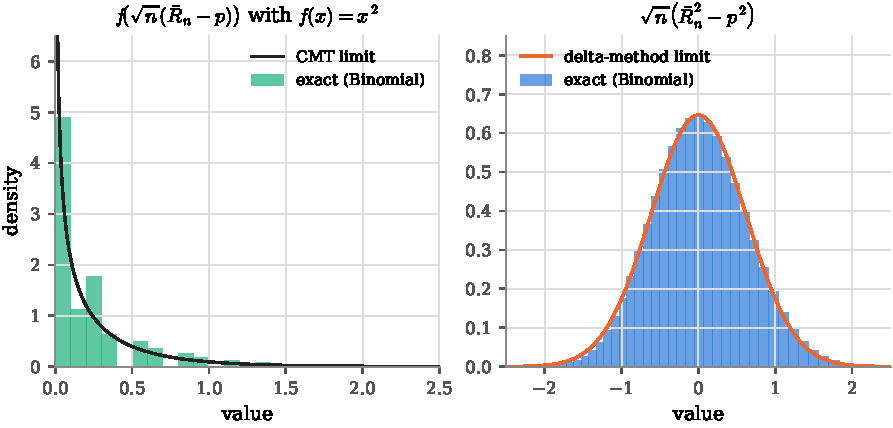
\includegraphics[width=\textwidth]{fig_cmt_pitfall}
\caption{Two different random variables for $f(x) = x^2$ in the kiss model, $p = 0.645$, $n = 124$. Left: $(\sqrt{n}(\bar{R}_n - p))^2$ with its CMT limit (black curve). Right: $\sqrt{n}(\bar{R}_n^2 - p^2)$ with its delta-method limit (orange curve). The bars are the exact Binomial distribution of $n\bar{R}_n$, binned.}
\label{fig:cmtpitfall}
\end{figure}

\section{The delta method}
\label{sec:delta-method}

The delta method is what you need when you're taking the limit of something like $\sqrt{n} \left( g(\bar{X}_n) - g(\mu) \right)$: you know the CLT for $\bar{X}_n$, and you want the CLT for a function of it.

\begin{theorem}[Delta method]
\label{thm:delta}
Let $(Z_n)_{n \geq 1}$ be a sequence of r.v.s such that:
\[
\sqrt{n} (Z_n - \theta) \convd \Gauss(0, \sigma^2),
\]
for some $\theta \in \real$ and $\sigma^2 > 0$.
A sequence like $(Z_n)_{n \geq 1}$ that satisfies this condition is said to be \textit{asymptotically normal around} $\theta$, and $\sigma^2$ is its asymptotic variance.
Let $g: \real \to \real$ be continuously differentiable at the point $\theta$.
Then:
\begin{enumerate}[nosep]
\item $g(Z_n) \convp g(\theta)$;
\item $(g(Z_n))_{n \geq 1}$ is also asymptotically normal, around $g(\theta)$;
\item more precisely,
\[
\sqrt{n} \left( g(Z_n) - g(\theta) \right) \convd \Gauss \left( 0, \, g'(\theta)^2 \sigma^2 \right).
\]
\end{enumerate}
\end{theorem}

\begin{intuition}[a differentiable function is locally linear]
\Cref{fig:delta} is the whole idea.
It is drawn for $g(x) = 1/x$ with the numbers of the subway example below, $\theta = 6.23$ and $\sigma/\sqrt{n} = 0.78$; the dotted lines map $\theta \pm 2\sigma/\sqrt{n}$ across.
For large $n$, $Z_n$ sits in a narrow Gaussian blob of width $\sigma/\sqrt{n}$ around $\theta$.
On a blob that narrow, the curve $g$ is indistinguishable from its tangent line at $\theta$, which has slope $g'(\theta)$.
A linear function maps a Gaussian to a Gaussian, shifting the center to $g(\theta)$ and multiplying the width by the slope.
So $g(Z_n)$ sits in a Gaussian blob of width $\abs{g'(\theta)} \, \sigma / \sqrt{n}$ around $g(\theta)$, which is statement (3).
Where $g$ is steep, errors in $Z_n$ are amplified; where it's flat, they're damped.
\end{intuition}

\begin{figure}[htbp]
\centering
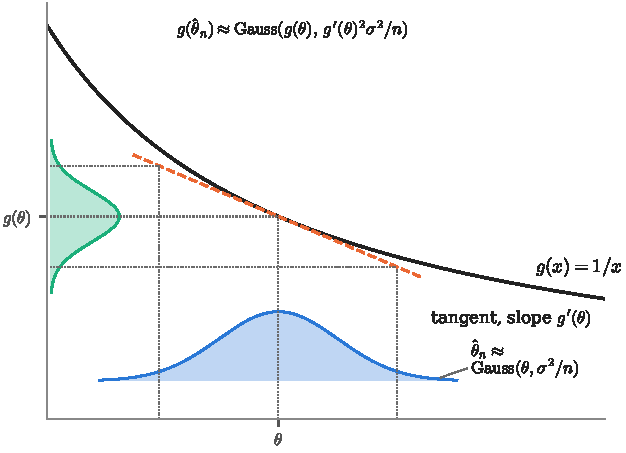
\includegraphics[width=0.78\textwidth]{fig_delta_method}
\caption{The delta method for $g(x) = 1/x$, $\theta = 6.23$, $\sigma/\sqrt{n} = 0.78$: the input Gaussian in blue on the horizontal axis, its image in green on the vertical axis, the tangent at $\theta$ dashed in orange, and dotted guides at $\theta \pm 2\sigma/\sqrt{n}$.}
\label{fig:delta}
\end{figure}

\coreproof{The mean value theorem \toolkit{sec:math-mvt} writes $g(Z_n) - g(\theta)$ as a slope times $Z_n - \theta$. The slope converges in probability to $g'(\theta)$ (CMT), and $\sqrt{n}(Z_n - \theta)$ converges in distribution (the assumption); Slutsky multiplies the two.}
\begin{proof}
By the mean value theorem there's a point $\tilde{\theta}_n$ between $Z_n$ and $\theta$ such that
\[
g(Z_n) - g(\theta) = g'(\tilde{\theta}_n)(Z_n - \theta).
\]
Multiply through by $\sqrt{n}$:
\[
\sqrt{n} \left( g(Z_n) - g(\theta) \right) = g'(\tilde{\theta}_n) \cdot \sqrt{n}(Z_n - \theta).
\]
Now take the two factors in turn.
First, $Z_n \convp \theta$: by Slutsky, $Z_n - \theta = \frac{1}{\sqrt{n}} \cdot \sqrt{n}(Z_n - \theta) \convd 0 \cdot \Gauss(0, \sigma^2) = 0$, and convergence in distribution to a constant is convergence in probability (\cref{prop:convd-constant}).
This proves (1) via the CMT, and since $\tilde{\theta}_n$ is squeezed between $Z_n$ and $\theta$, also $\tilde{\theta}_n \convp \theta$, hence $g'(\tilde{\theta}_n) \convp g'(\theta)$ by the CMT and the continuity of $g'$ at $\theta$.
Second, $\sqrt{n}(Z_n - \theta) \convd \Gauss(0, \sigma^2)$ by assumption.
Slutsky's multiplicative property with $y = g'(\theta)$ gives
\[
g'(\tilde{\theta}_n) \cdot \sqrt{n}(Z_n - \theta) \convd g'(\theta) \cdot \Gauss(0, \sigma^2) = \Gauss(0, g'(\theta)^2 \sigma^2),
\]
which is (3), and (2) is (3) read as a sentence.
\end{proof}

The proof is three lines because Slutsky and the CMT did the work in advance.
Note that nothing requires $g$ to be invertible or monotone; $g(x) = \sqrt{2} \sin x$ is a perfectly good choice.
Note also that the asymptotic variance $g'(\theta)^2 \sigma^2$ generally depends on the unknown $\theta$, even when $\sigma^2$ doesn't; the plug-in trick of the previous section handles that.

\begin{worked}[inter-arrival times of the T]
You observe the times between arrivals of the subway at Kendall, $T_1, \ldots, T_n$, and model them as i.i.d.\ $\Expo(\lambda)$, so $\E[T_1] = 1/\lambda$ and $\var(T_1) = 1/\lambda^2$.
The natural estimator of $\lambda$ is $\hat{\lambda} = 1/\bar{T}_n$.
\begin{itemize}[nosep]
\item \textit{Consistency.} $\bar{T}_n \convp 1/\lambda$ by the Law of Large Numbers, so $\hat{\lambda} = 1/\bar{T}_n \convp \lambda$ by the CMT ($f(x) = 1/x$ is continuous at $1/\lambda > 0$).
\item \textit{The CLT for $\bar{T}_n$.} $\sqrt{n} \left( \bar{T}_n - \frac{1}{\lambda} \right) \convd \Gauss(0, \lambda^{-2})$.
\item \textit{The delta method for $\hat{\lambda}$.} Take $g(x) = 1/x$, so $g'(x) = -1/x^2$ and $g'(1/\lambda)^2 = \lambda^4$. Then
\[
\sqrt{n} \left( \hat{\lambda} - \lambda \right) \convd \Gauss \left( 0, \, \lambda^4 \cdot \lambda^{-2} \right) = \Gauss(0, \lambda^2).
\]
\end{itemize}
With $n = 64$ and $\bar{T}_n = 6.23$ minutes: $\hat{\lambda} = 0.1605$ per minute, and the standard error of $\hat{\lambda}$ (the standard deviation $\lambda/\sqrt{n}$ of its approximating Gaussian, with $\hat{\lambda}$ plugged in for $\lambda$) is about $0.020$.
So $\lambda$ is pinned down to roughly $0.16 \pm 0.04$, which becomes the plug-in confidence interval $[0.12, 0.20]$ of \cref{ch:confidence-intervals}.
\end{worked}

\begin{worked}[odds in the kiss experiment]
The odds of turning right are $\omega = p/(1-p)$, estimated by $\hat{\omega} = \bar{R}_n/(1 - \bar{R}_n)$.
With $g(p) = p/(1-p)$ you get $g'(p) = 1/(1-p)^2$, and the CLT gives asymptotic variance $p(1-p)$ for $\bar{R}_n$, so
\[
\sqrt{n} \left( \hat{\omega} - \omega \right) \convd \Gauss \left( 0, \, \frac{p(1-p)}{(1-p)^4} \right) = \Gauss \left( 0, \, \frac{p}{(1-p)^3} \right).
\]
At $p = 0.645$ and $n = 124$: $\hat{\omega} = 1.82$ and the standard error is $\sqrt{0.645/0.355^3/124} \approx 0.34$.
The derivative $1/(1-p)^2 \approx 7.9$ is large, so the odds are estimated far less precisely, in absolute terms, than the proportion they're computed from: a steep $g$ amplifies the error.
\Cref{fig:steepflat} puts this next to a flat $g$, where the same input error nearly disappears.
The input on both sides is $\bar{R}_n \approx \Gauss(p, p(1-p)/n)$ with standard deviation $0.043$.
On the left, the odds have slope $7.9$ at $p = 0.645$, and the output standard deviation is $7.9 \times 0.043 = 0.34$.
On the right, the variance $g(p) = p(1-p)$ has slope $-0.29$ there, and the output standard deviation is $0.29 \times 0.043 = 0.012$.
Same data and the same precision in $p$; the delta method's $\abs{g'(\theta)}$ is the whole difference in the precision of $g(p)$.
\end{worked}

\begin{figure}[htbp]
\centering
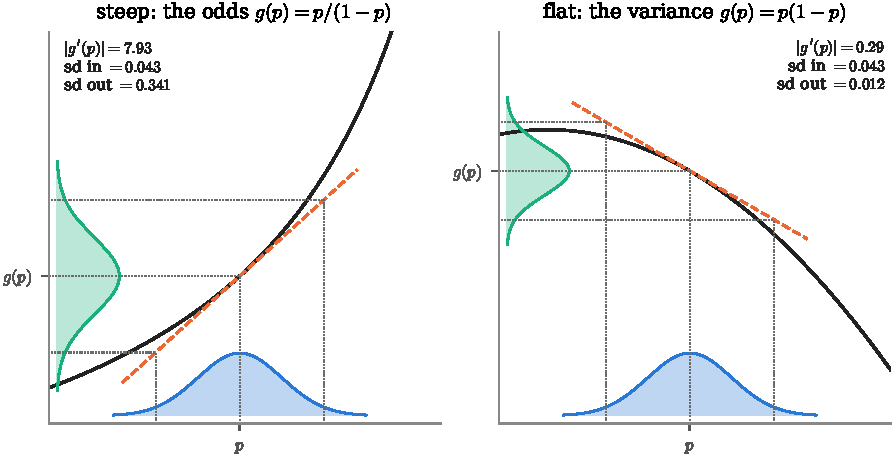
\includegraphics[width=\textwidth]{fig_delta_steep_flat}
\caption{The input $\bar{R}_n \approx \Gauss(p, p(1-p)/n)$, in blue on the horizontal axis, pushed through two functions, with the output in green on the vertical axis and the tangent at $p$ dashed in orange. Left: the odds $g(p) = p/(1-p)$. Right: the variance $g(p) = p(1-p)$.}
\label{fig:steepflat}
\end{figure}

\begin{bridge}[propagation of error]
If you took a laboratory course you met the rule `if $y = g(x)$ and $x$ has uncertainty $\delta x$, then $y$ has uncertainty $\delta y \approx \abs{g'(x)} \, \delta x$'.
The delta method is that rule for standard errors, with a theorem attached:
\[
\se \left( g(\ethn) \right) \approx \abs{g'(\theta)} \, \se(\ethn), \qquad \se(\ethn) = \frac{\sigma}{\sqrt{n}}.
\]
It also says what the lab rule leaves out: the transformed estimate isn't just `uncertain by $\delta y$', it's approximately Gaussian, so you can attach a probability to the error bar.
\end{bridge}

\begin{remark}
When $g'(\theta) = 0$ the theorem still holds but says only that $\sqrt{n}(g(Z_n) - g(\theta)) \convd 0$, that is, the error of $g(Z_n)$ is of smaller order than $1/\sqrt{n}$.
To see the actual limit you magnify by $n$ instead of $\sqrt{n}$ and get a second-order expansion: $n(g(Z_n) - g(\theta)) \convd \frac{\sigma^2 g''(\theta)}{2} \chi^2_1$.
No result later in this book needs this case.
\end{remark}

\begin{remark}[Vector versions]
Everything in this chapter has a version for vectors, with a covariance matrix in place of $\sigma^2$ and a matrix of partial derivatives in place of $g'(\theta)$.
If $\sqrt{n}(Z_n - \theta) \convd \Gauss_d(0, \Sigma)$ and $g: \real^d \to \real^k$ is continuously differentiable at $\theta$, with $\nabla g(\theta)$ the $d \times k$ matrix of partial derivatives, then
\[
\sqrt{n} \left( g(Z_n) - g(\theta) \right) \convd \Gauss_k \left( 0, \, \nabla g(\theta)^\top \Sigma \, \nabla g(\theta) \right),
\]
and the multivariate CLT says that the vector of sample means of i.i.d.\ vectors with covariance $\Sigma$ satisfies the hypothesis with $\Sigma$ itself.
The proofs are the ones above with matrices in place of numbers.
The method of moments (\cref{ch:mom-mestimation}) and the chi-squared goodness-of-fit test (\cref{ch:gof}) use these, and the book states them again there in the form each needs.
\end{remark}

\begin{bridge}[the confidence interval for an odds ratio]
Courses in biostatistics and epidemiology teach a confidence interval for an odds ratio: the log of the estimated odds ratio plus or minus $1.96\sqrt{1/a + 1/b + 1/c + 1/d}$, with $a, b, c, d$ the four counts of the two-by-two table, exponentiated at both ends.
The square root is the delta method.
For one group with $S$ successes in $n$ trials, the log odds $g(p) = \log\big(p/(1-p)\big)$ has $g'(p) = 1/\big(p(1-p)\big)$, so \cref{thm:delta} gives it approximate variance $g'(p)^2 \, p(1-p)/n = \big(1/p + 1/(1-p)\big)/n$, which with $\hat{p} = S/n$ plugged in is $1/S + 1/(n - S)$.
For the kiss data the log odds of turning right is $\log(80/44) = 0.598$ with standard error $\sqrt{1/80 + 1/44} = 0.188$, and exponentiating the ends of $0.598 \pm 1.96 \times 0.188$, which keeps the level (\cref{sec:ci-subway}), gives $[1.26, 2.63]$ for the odds.
An odds ratio compares two independent groups, so its log is the difference of two independent log odds, and the variance of that difference adds all four reciprocals.
\end{bridge}

\section{Where the limit theorems are used in the rest of the book}
\label{sec:conv-where-used}

Every asymptotic statement in the later chapters is one of the facts of \cref{ch:lln,ch:clt} or this chapter in disguise, with two exceptions the table names, both stated without proof (Donsker's theorem about the whole empirical CDF, behind the Kolmogorov--Smirnov test, and the Bernstein--von Mises theorem of \cref{ch:bayes-intro}).
The table says which.
`LLN' means the Law of Large Numbers (\cref{thm:wlln}), `CLT' the Central Limit Theorem (\cref{thm:clt}), `CMT' the continuous mapping theorem (\cref{thm:cmt}), `Slutsky' \cref{thm:slutsky}, and `delta' the delta method (\cref{thm:delta}).

\begin{center}
\small
\begin{tabular}{@{}>{\raggedright\arraybackslash}p{2.55in}>{\raggedright\arraybackslash}p{0.9in}>{\raggedright\arraybackslash}p{2.45in}@{}}
\toprule
Result & Chapter & Rests on \\
\midrule
Consistency of $\bar{X}_n$, $\hat{p}$, and any estimator built from an average & \cref{ch:estimators} & LLN, then CMT for functions of averages \\[3pt]
Asymptotic confidence intervals; the plug-in interval & \cref{ch:confidence-intervals} & CLT; Slutsky for replacing $p$ by $\hat{p}$ in the standard error \\[3pt]
Confidence interval for $1/\bar{T}_n$ and other transformed estimators & \cref{ch:confidence-intervals} & delta \\[3pt]
Level and $p$-value of a test built on a standardized average & \cref{ch:tests-foundations} & CLT, Slutsky \\[3pt]
Consistency of the maximum likelihood estimator & \cref{ch:mle-properties} & LLN applied to the average log-likelihood, plus the KL divergence argument \\[3pt]
Asymptotic normality of the MLE, with variance $1/I(\theta)$ & \cref{ch:mle-properties} & CLT applied to the average score, then a Taylor expansion exactly as in the delta method proof, with Fisher information as the slope \\[3pt]
Method of moments: consistency and asymptotic variance & \cref{ch:mom-mestimation} & LLN, then the (multivariate) delta method \\[3pt]
Wald test & \cref{ch:wald-lrt} & asymptotic normality of the MLE, Slutsky for the estimated information, CMT (squaring gives a $\chi^2$) \\[3pt]
Likelihood ratio test (Wilks' theorem) & \cref{ch:wald-lrt} & a second-order Taylor expansion, the same device as the delta method, plus Slutsky \\[3pt]
Score test & \cref{ch:wald-lrt} & multivariate CLT applied to the score, then CMT \\[3pt]
$t$-test & \cref{ch:t-test} & nothing here: exact for Gaussian data (Cochran's theorem) \\[3pt]
Chi-squared goodness-of-fit test & \cref{ch:gof} & multivariate CLT for the rotated standardized deviations of the counts, then CMT; with estimated parameters, the nuisance-parameter theorem of \cref{ch:wald-lrt} \\[3pt]
Kolmogorov--Smirnov and Lilliefors tests & \cref{ch:ks} & Glivenko--Cantelli (a uniform LLN), proved there from the LLN at finitely many points; Donsker's theorem (a CLT for the whole empirical CDF), stated without proof \\[3pt]
Bayesian posteriors concentrate on the truth (proved for Beta priors); Bernstein--von Mises & \cref{ch:bayes-intro} & LLN and Chebyshev for the concentration; Bernstein--von Mises stated, not proved \\[3pt]
Inference for least squares with non-Gaussian errors & \cref{ch:regression-multi} & CLT (exact $t$ and $F$ when errors are Gaussian) \\[3pt]
Asymptotic normality of GLM estimates & \cref{ch:glm-links} & the MLE result again \\[3pt]
Sample covariance converges to the true covariance & \cref{ch:pca} & LLN entrywise, then CMT for the eigenvectors \\
\bottomrule
\end{tabular}
\end{center}

\section{What comes next}
\label{sec:tools-next}

Every limit in these three chapters landed on the same distribution.
\Cref{ch:gaussian} collects what the rest of the book needs about it: the density, the three properties that let you standardize anything Gaussian, how to turn a Gaussian probability into a table lookup, and this book's convention for quantiles, which is the notation every confidence interval and test from \cref{ch:confidence-intervals} on is written in.
If you know the Gaussian well, the quantile section is the one part not to skip.

\section{Summary}
\label{sec:tools-summary}

\begin{itemize}[nosep]
\item For convergence in probability (and almost surely), limits add, multiply and divide like limits of numbers. For convergence in distribution they do not: the marginal limits of $X_n$ and $Y_n$ don't determine the limit of $X_n + Y_n$.
\item \textbf{Slutsky's theorem:} if $X_n \convd X$ and $Y_n \convp y$ with $y$ a constant, then $X_n + Y_n \convd X + y$, $X_n Y_n \convd yX$ and $X_n / Y_n \convd X/y$. This justifies every plug-in: replacing $\sigma$ by $s$, or $p$ by $\hat{p}$, in a standard error.
\item \textbf{Continuous mapping theorem:} $X_n \to X$ in any of the three modes implies $f(X_n) \to f(X)$ in the same mode, for $f$ continuous at the limit. Consistency survives transformations. What it does not give you is the limit of $\sqrt{n}(f(\bar{X}_n) - f(\mu))$; that is the delta method's job.
\item \textbf{Delta method:} if $\sqrt{n}(Z_n - \theta) \convd \Gauss(0, \sigma^2)$ and $g$ is continuously differentiable at $\theta$, then $\sqrt{n}(g(Z_n) - g(\theta)) \convd \Gauss(0, g'(\theta)^2 \sigma^2)$. A narrow Gaussian blob pushed through a smooth curve comes out Gaussian, with its width multiplied by the slope. This is propagation of error with a theorem attached.
\end{itemize}

\section{Exercises}
\label{sec:tools-exercises}

\begin{exercise}
Let $\Xton \iid \Bern(p)$. Use the delta method to find the asymptotic distribution of $\sqrt{n} \left( \bar{X}_n(1 - \bar{X}_n) - p(1-p) \right)$. For which $p$ does the delta method fail to give a Gaussian limit, and why?
\end{exercise}
\begin{solution}
With $g(p) = p(1-p)$, $g'(p) = 1 - 2p$, and the CLT gives asymptotic variance $p(1-p)$ for $\bar{X}_n$, so the limit is $\Gauss(0, (1-2p)^2 p(1-p))$. At $p = \frac12$ the derivative is $0$ and the limit is degenerate: the sample variance of a fair coin is estimated with error of order $1/n$ rather than $1/\sqrt{n}$, and the second-order remark of \cref{sec:delta-method} applies.
\end{solution}

\begin{exercise}
Let $\Xton \iid \Expo(\lambda)$. Show that $\sqrt{n}(\log \bar{X}_n + \log \lambda) \convd \Gauss(0, 1)$, whatever $\lambda$ is. Why might a statistician prefer to build a confidence interval for $\log(1/\lambda)$ rather than for $1/\lambda$?
\end{exercise}
\begin{solution}
The CLT gives $\sqrt{n}(\bar{X}_n - 1/\lambda) \convd \Gauss(0, 1/\lambda^2)$. With $g(x) = \log x$, $g'(1/\lambda) = \lambda$, so the asymptotic variance of $\log \bar{X}_n$ is $\lambda^2 \cdot \lambda^{-2} = 1$, free of $\lambda$. A limit whose variance doesn't depend on the unknown parameter needs no plug-in: the interval $\log \bar{X}_n \pm 1.96/\sqrt{n}$ for $\log(1/\lambda)$ has asymptotic level $95\%$ with no further work, and can be exponentiated afterwards. This is called a variance-stabilizing transformation.
\end{solution}

\begin{exercise}
Let $\Xton \iid \Bern(p)$ with $0 < p < 1$. Show that
\[
\sqrt{n}\,\frac{\bar{X}_n - p}{\sqrt{\bar{X}_n(1 - \bar{X}_n)}} \convd \Gauss(0,1),
\]
naming the theorem used at each step.
\end{exercise}
\begin{solution}
By the CLT, $\sqrt{n}(\bar{X}_n - p)/\sqrt{p(1-p)} \convd \Gauss(0,1)$. By the LLN, $\bar{X}_n \convp p$, and $x \mapsto \sqrt{p(1-p)/(x(1-x))}$ is continuous at $p$, so by the continuous mapping theorem $\sqrt{p(1-p)/(\bar{X}_n(1-\bar{X}_n))} \convp 1$. Slutsky's multiplicative property with $y = 1$ gives the product's limit, $1 \cdot \Gauss(0,1)$.
\end{solution}

\chapter{The Gaussian Distribution and Quantiles}
\label{ch:gaussian}

\begin{chaptergoals}
\begin{itemize}[nosep]
\item The Gaussian density: what each piece of the formula does, why the CDF has no closed form, and why the tails are so thin that the distribution lives in a finite interval for practical purposes.
\item The three properties used constantly from here on: closure under affine transformations, standardization, and symmetry. Plus the one that usually goes unstated: sums of independent Gaussians are Gaussian.
\item How to turn a Gaussian probability into a table lookup, forwards and backwards.
\item Quantiles, in this book's convention $q_\alpha$ (the number with mass $\alpha$ to its \textit{right}), the four values worth memorizing, and the one-sided versus two-sided distinction that every confidence interval and test depends on.
\end{itemize}
This chapter is a review. If you know it, read the quantile section for the notation and move on.
\end{chaptergoals}

\section{Why the Gaussian is everywhere}
\label{sec:gauss-why}

\Cref{ch:lln,ch:clt,ch:limit-tools} kept producing Gaussian limits; this chapter collects what you need about the Gaussian to use them, and fixes the quantile notation of the rest of the book.
Because of the Central Limit Theorem (\cref{ch:clt}), the Gaussian (also called the normal) distribution is ubiquitous in statistics: every average of enough independent, identically distributed draws with finite variance is approximately Gaussian, whatever the draws come from, so every estimator built from an average inherits a Gaussian error distribution for large $n$.
That is where the Gaussian enters statistical inference, and it stays: confidence intervals, test statistics, the asymptotic distribution of the maximum likelihood estimator, the error term of linear regression.
The distribution is named after Carl Friedrich Gauss (1777--1855), who arrived at it in the context of the method of least squares, which is the subject of \cref{ch:regression-uni}.

\section{The density and its CDF}
\label{sec:gauss-density}

\begin{definition}[Gaussian distribution]
\label{def:gaussian}
A continuous r.v.\ $X$ has the \textbf{Gaussian distribution} with parameters $\mu \in \real$ and $\sigma^2 > 0$ if its PDF is given by:
\[
f_{\mu, \sigma^2}(x) = \frac{1}{\sigma \sqrt{2 \pi}} \exp \left(- \frac{(x - \mu)^2}{2 \sigma^2} \right), \, \text{ for } x \in (-\infty, \infty).
\]
You write this as $X \sim \Gauss(\mu, \sigma^2)$, and then $\E[X] = \mu$ and $\var(X) = \sigma^2$.
The case $\mu = 0$, $\sigma^2 = 1$ is the \textbf{standard Gaussian}, whose density and CDF get their own letters:
\[
\varphi(z) = \frac{1}{\sqrt{2\pi}} e^{-z^2/2}, \qquad \Phi(z) = \int_{-\infty}^z \varphi(t) \, \mathrm{d}t.
\]
\end{definition}

\begin{inwords}
\textbf{In words.} A Gaussian variable is one whose probabilities are areas under the bell-shaped curve above \toolkit{sec:math-density}; $\mu$ says where the bell is centered and $\sigma$ how wide it is. Two numbers fix the whole distribution.
\par\smallskip
\textbf{For the kiss data.} The CLT says $\bar{R}_n$ behaves, for large $n$, like a Gaussian with $\mu = p$ and $\sigma^2 = p(1-p)/n$: centered at the truth, with width $0.043$ at $n = 124$ and $p = 0.645$.
\end{inwords}

Take the formula apart.
The constant $\ds \frac{1}{\sigma \sqrt{2 \pi}}$ is a \textit{normalizing constant}: it normalizes the total area under the PDF to 1, and plays no other role.
Everything about the shape is in the exponent.
Consider the quadratic there:
\[
- \frac{(x - \mu)^2}{2\sigma^2} = - \left( \frac{x^2 - 2\mu x + \mu^2}{2\sigma^2} \right).
\]
It is zero at $x = \mu$ and negative everywhere else, so the density peaks at $\mu$ and falls off symmetrically on both sides.
If $\sigma$ is small, that is, if the standard deviation is small, then the quadratic is more negative at the same distance from $\mu$, so the exponential falls off faster and the density is narrower.
A small standard deviation and a narrow density are the same thing seen twice.
\Cref{fig:gaussdensity} shows the effect of each parameter.
On the left, $\Gauss(0, 4)$ is $\Gauss(0, 1)$ stretched to twice the width, and its peak drops to half the height to keep the area at $1$; $\Gauss(10, 4)$ is $\Gauss(0, 4)$ moved ten units to the right with no change of shape.
So $\mu$ moves the density without changing its shape, and $\sigma$ stretches it without moving its center.
On the right, the three shaded regions of the standard Gaussian have probabilities $0.6827$, $0.9545$ and $0.9973$: the `$68$--$95$--$99.7$ rule' of an introductory course, stated exactly.

\begin{figure}[htbp]
\centering
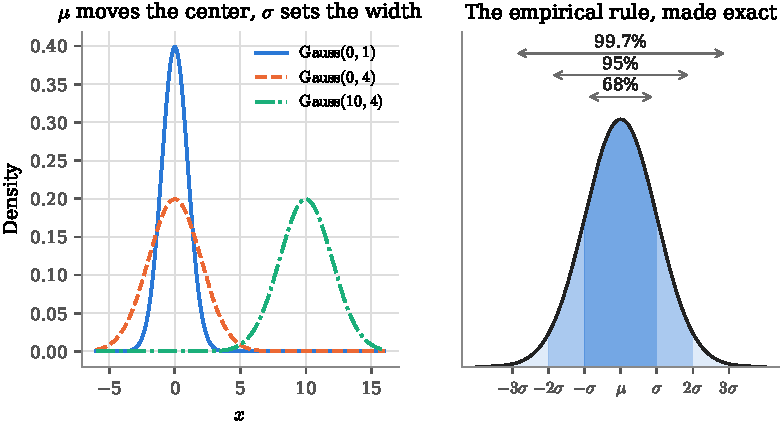
\includegraphics[width=\textwidth]{fig_gaussian_density}
\caption{Left: the densities of $\Gauss(0, 1)$ (solid), $\Gauss(0, 4)$ (dashed) and $\Gauss(10, 4)$ (dash-dot). Right: the standard Gaussian density, shaded within one, two and three standard deviations of the mean.}
\label{fig:gaussdensity}
\end{figure}

Two consequences of the exponent are worth stating on their own.
\begin{itemize}
\item \textbf{The tails are thin.}
The density decays like $e^{-x^2/(2\sigma^2)}$, faster than any exponential $e^{-c|x|}$, so for practical purposes a Gaussian lives in a finite interval: $99.7\%$ of the mass is within $3\sigma$ of $\mu$, and the probability of being more than $5\sigma$ away is about one in two million.
This is what licenses a statement like `with overwhelming probability $\abs{\bar{X}_n - \mu} \leq 3\sigma/\sqrt{n}$' (\cref{sec:clt}).
\item \textbf{The CDF has no closed form.}
\[
\Pr(X \leq x) = F_{\mu, \sigma^2}(x) = \frac{1}{\sigma \sqrt{2\pi}} \int_{-\infty}^x \exp \left(- \frac{(t - \mu)^2}{2 \sigma^2} \right) \, \mathrm{d}t
\]
must be left as an integral: it's mathematically impossible to write the antiderivative of $e^{-t^2/2}$ in terms of elementary functions.
Still, $F_{\mu, \sigma^2}$ is a perfectly well-defined function: input some value $x$ and it returns the accumulated area under the PDF from $-\infty$ up to $x$.
You get its values from tables or from software, and \cref{sec:gauss-computing} says how.
\end{itemize}

\section{Properties of Gaussian distributions}
\label{sec:gauss-properties}

\begin{enumerate}
\item \textbf{Affine transformation.}
Perhaps the most useful property of the Gaussian family is that it is invariant under affine transformations.
Given the r.v.\ $X \sim \Gauss(\mu, \sigma^2)$, then
\[
aX + b \sim \Gauss(a\mu + b, a^2\sigma^2) \qquad \text{for all } a \neq 0, \, b \in \real.
\]
Shifting and rescaling a Gaussian produces another Gaussian; the mean and variance change in the way means and variances always do under $aX + b$, and the shape stays Gaussian, which is the content of the statement.

\optionalproof{Write the CDF of $aX + b$ as a CDF of $X$ at a transformed point, differentiate (chain rule) to get the density, and recognize the Gaussian formula with new parameters \toolkit{sec:math-density}.}
\begin{proof}
Take $a > 0$ (the case $a < 0$ is the same with the inequality flipped).
The CDF of $Y = aX + b$ is
\[
F_Y(y) = \Pr(aX + b \leq y) = \Pr \left( X \leq \frac{y - b}{a} \right) = F_X \left( \frac{y-b}{a} \right).
\]
Differentiate with respect to $y$ (chain rule) to get the density:
\begin{align*}
f_Y(y) = \frac{1}{a} f_X \left( \frac{y - b}{a} \right) &= \frac{1}{a \sigma \sqrt{2\pi}} \exp \left( - \frac{\left( \frac{y-b}{a} - \mu \right)^2}{2 \sigma^2} \right) \\
&= \frac{1}{(a\sigma) \sqrt{2\pi}} \exp \left( - \frac{(y - (a\mu + b))^2}{2 (a\sigma)^2} \right),
\end{align*}
which is the $\Gauss(a\mu + b, a^2 \sigma^2)$ density.
\end{proof}

\item \textbf{Standardization.}
If $X \sim \Gauss(\mu, \sigma^2)$, then:
\[
Z = \frac{X - \mu}{\sigma} \sim \Gauss(0, 1).
\]
This is the affine property with $a = 1/\sigma$ and $b = -\mu/\sigma$, and it is the single most used fact about the Gaussian because it reduces every Gaussian probability to a probability about the one fixed distribution that is tabulated.
That is because of standardization, you have that:
\[
\Pr(u \leq X \leq v) = \Pr \left( \frac{u - \mu}{\sigma} \leq Z \leq \frac{v-\mu}{\sigma}\right) = \Phi \left( \frac{v-\mu}{\sigma} \right) - \Phi \left( \frac{u-\mu}{\sigma} \right),
\]
where $Z$ on the right-hand side is as above, $Z = \frac{X - \mu}{\sigma}$.

\textbf{Question:} Why does this last result follow?

\textbf{Answer:} Consider $\Pr(u \leq X \leq v)$ where $X \sim \Gauss(\mu, \sigma^2)$.
First, mean-center the variables by subtracting the mean of $X$ in the inequalities and then divide each term by the standard deviation.
\begin{align*}
\Pr(u \leq X \leq v) &= \Pr(u - \mu \leq X - \mu \leq v - \mu) \\
					 &= \Pr \left( \frac{u - \mu}{\sigma} \leq \frac{X - \mu}{\sigma} \leq \frac{v - \mu}{\sigma} \right) \\
					 &= \Pr \left( \frac{u - \mu}{\sigma} \leq Z \leq \frac{v - \mu}{\sigma} \right).
\end{align*}
Observe that the inequalities are preserved because adding a number and multiplying by a positive number doesn't change an inequality's direction.

\item \textbf{Symmetry.}
If $X \sim \Gauss(0, \sigma^2)$, then $-X \sim \Gauss(0, \sigma^2)$ (the affine property with $a = -1$, $b = 0$).
Consequently, for $x > 0$:
\begin{align*}
\Pr(\abs{X} > x) &= \Pr(X > x \text{ or } X < -x) \\
				&= \Pr(X > x) + \Pr(X < -x) \\
				&= \Pr(X > x) + \Pr(-X > x) \\
				&= 2 \Pr(X > x).
\end{align*}
Intuitively, when you negate a Gaussian r.v.\ you mirror its distribution about the vertical axis.
This mirroring doesn't change the shape or the spread of the distribution; it only changes the sign of the values.
As a result, the negated Gaussian random variable $-X$ maintains the same mean (here, 0) and the same variance $\sigma^2$ as the original r.v.\ $X$.
For the standard Gaussian the symmetry reads $\Phi(-z) = 1 - \Phi(z)$, which is why tables only print positive $z$.

\item \textbf{Sums of independent Gaussians are Gaussian.}
If $X_1 \sim \Gauss(\mu_1, \sigma_1^2)$ and $X_2 \sim \Gauss(\mu_2, \sigma_2^2)$ are independent, then
\[
X_1 + X_2 \sim \Gauss(\mu_1 + \mu_2, \sigma_1^2 + \sigma_2^2).
\]
The mean and variance are what they would be for any independent pair; the point is again that the shape stays Gaussian.
(The proof is omitted here; it follows from the convolution formula, or in one line from moment generating functions.)
Combined with the affine property, it gives the fact behind every exact small-sample result in this book: if $\Xton \iid \Gauss(\mu, \sigma^2)$ then
\[
\bar{X}_n \sim \Gauss \left( \mu, \frac{\sigma^2}{n} \right) \qquad \text{exactly, for every } n,
\]
with no appeal to the Central Limit Theorem.
For Gaussian data the CLT's conclusion holds at $n = 2$.
\end{enumerate}

\begin{bridge}[$z$-scores]
Standardization is the $z$-score of an introductory course: `how many standard deviations above the mean is this observation?'
What the introductory course sometimes leaves unsaid is that the $z$-score of a Gaussian observation is itself a standard Gaussian random variable, which is the reason a single table serves every $\mu$ and $\sigma$.
Here the same move is applied not to an observation but to an estimator: $\sqrt{n}(\bar{X}_n - \mu)/\sigma$ is the $z$-score of $\bar{X}_n$, and the CLT says it is approximately standard Gaussian.
Every `$z$-interval' and `$z$-test' you learned is that sentence plus a quantile from \cref{sec:gauss-quantiles}.
\end{bridge}

\section{Computing probabilities, forwards and backwards}
\label{sec:gauss-computing}

Since the CDF has no formula, every Gaussian probability is computed by standardizing and then looking up $\Phi$, in a table or in software.
There are two directions.
\textit{Forwards:} given a value, find a probability; standardize to a $z$-score and read $\Phi(z)$.
\textit{Backwards:} given a probability, find the value; read the table in reverse to get $z = \Phi^{-1}(\text{probability})$ and unstandardize, $x = \mu + \sigma z$.
\Cref{fig:gausscdf} shows both on the graph of $\Phi$, with the numbers of the exam example that follows.
Forwards, a $z$-score goes in on the horizontal axis and a probability comes out on the vertical axis: $\Phi(2.5) = 0.9938$.
Backwards, a probability goes in on the vertical axis and a $z$-score comes out on the horizontal axis: $\Phi^{-1}(0.90) = 1.28$.
Tables print the forward direction; for the backward direction you scan the table for the probability, or ask software for the quantile directly.

\begin{figure}[htbp]
\centering
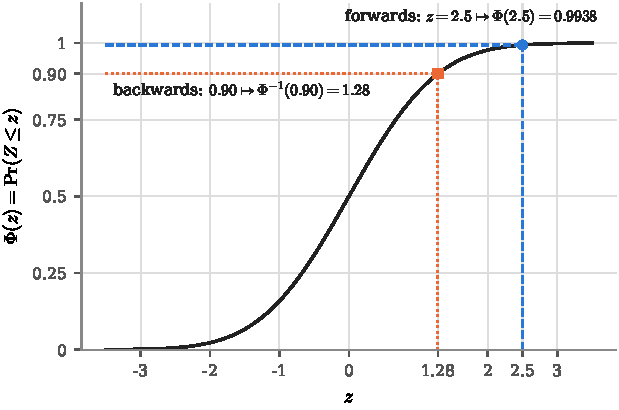
\includegraphics[width=0.72\textwidth]{fig_gaussian_cdf}
\caption{The standard Gaussian CDF $\Phi$ with the two readings of the exam example below: forwards from $z = 2.5$ to $\Phi(2.5) = 0.9938$ (blue dashes), backwards from $0.90$ to $\Phi^{-1}(0.90) = 1.28$ (orange dots).}
\label{fig:gausscdf}
\end{figure}

\begin{worked}[exam scores]
Assume that the score distribution for a final exam is approximately $X \sim \Gauss(85, 4)$, that is, mean $85$ and standard deviation $\sigma = 2$.
\begin{itemize}[nosep]
\item $\Pr(X > 90)$. Standardize: $z = (90 - 85)/2 = 2.5$. Then $\Pr(X > 90) = \Pr(Z > 2.5) = 1 - \Phi(2.5) = 1 - 0.9938 = 0.0062$. About six students in a thousand score above $90$.
\item $\Pr(80 < X < 90)$. The endpoints standardize to $-2.5$ and $2.5$, so $\Pr(80 < X < 90) = \Phi(2.5) - \Phi(-2.5) = 2\Phi(2.5) - 1 = 0.9876$, using the symmetry $\Phi(-z) = 1 - \Phi(z)$.
\item The score $x$ such that $\Pr(X < x) = 0.90$ (the $90$th percentile). For this you read the table backwards: the $z$ with $\Phi(z) = 0.90$ is $z = 1.2816$, so $x = 85 + 2 \times 1.2816 = 87.6$.
\end{itemize}
\end{worked}

\begin{pitfall}[variance or standard deviation?]
This book writes $\Gauss(\mu, \sigma^2)$: the second parameter is the \textit{variance}.
So $\Gauss(85, 4)$ has standard deviation $2$, and $\Gauss(10, 4)$ in \cref{fig:gaussdensity} is twice as wide as $\Gauss(0, 1)$, not four times.
Most software and many textbooks take the standard deviation instead, and the mix-up fails silently: for the exam scores, $\Pr(X \leq 90)$ is $0.994$ with standard deviation $2$, but a $4$ entered where the $2$ was meant answers a different question and gives $0.894$, with no warning that anything went wrong.
Check which convention is in force every time, and when you write $\Gauss(\mu, \sigma^2)$ yourself, write the square.
\end{pitfall}

\section{Quantiles}
\label{sec:gauss-quantiles}

To grasp the idea of a quantile it's instructive to consider an example involving a closely related idea, a percentile.
Suppose you score a 72 on an exam.
Then your percentile is the fraction of students who score \textit{below} a 72.
In terms of probability, percentiles are computed using the CDF of exam scores: Letting $X$ denote the score of a random student on the exam, and to make things easy supposing $X$ is a continuous r.v., then your percentile is $\Pr(X \leq 72) = F_X(72)$.

In general, a student with score $x$ has percentile $F_X(x)$.
Going the other way, if you start with a percentile, say $0.95$, then $F^{-1}(0.95)$ is the score on the exam that has that percentile.
A percentile is also called a quantile, which is why $F^{-1}$ is called the \textbf{quantile function}.\footnote{More precisely, a percentile is a quantile expressed as a percentage.}
The function $F$ converts scores to quantiles, and the function $F^{-1}$ converts quantiles to scores: the forward and backward readings of \cref{fig:gausscdf}.
And finally, note that a quantile (of a specific order) is a number in the support of an r.v., not a probability.
Now for the formal definition, in the convention this book uses throughout.

\begin{definition}[Quantile of order $1 - \alpha$]
\label{def:quantile}
Let $\alpha \in (0,1)$.
The \textbf{quantile of order $1 - \alpha$} of an r.v.\ $X$ is the number $q_\alpha$ such that
\[
\Pr(X \leq q_\alpha) = 1 - \alpha.
\]
\end{definition}

\begin{figure}[htbp]
\centering
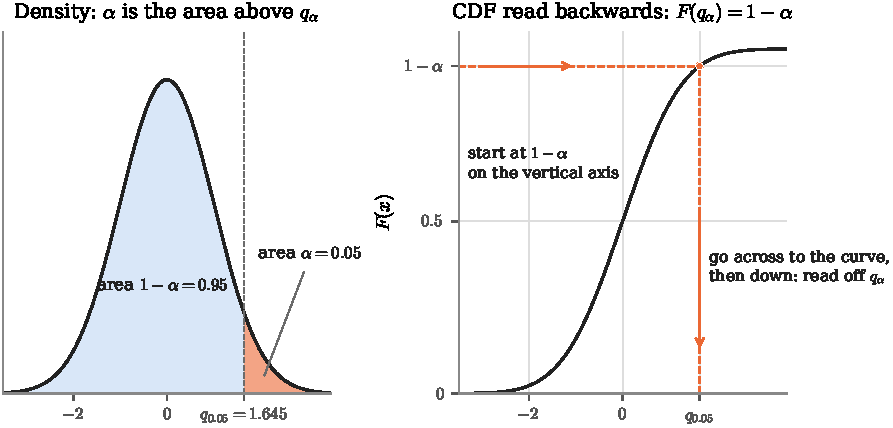
\includegraphics[width=\textwidth]{fig_quantile_def}
\caption{The definition of $q_\alpha$ for the standard Gaussian, $\alpha = 0.05$. Left: the density, with area $1 - \alpha$ below $q_\alpha$ (blue) and area $\alpha$ above it (orange). Right: the CDF, with the backward reading from $1 - \alpha$ to $q_\alpha$ (orange dashes).}
\label{fig:quantiledef}
\end{figure}

\begin{inwords}
\textbf{In words.} $q_\alpha$ is the cutoff with probability $\alpha$ above it and $1 - \alpha$ below: read the CDF backwards at $1 - \alpha$, as in \cref{fig:quantiledef} \toolkit{sec:math-density}. The subscript names the tail it cuts off, so read $q_{0.05}$ as `the cutoff with $5\%$ above it'.
\par\smallskip
\textbf{For the kiss data.} The $1.96$ in $\bar{R}_n \pm 1.96 \times 0.043$ is $q_{0.025}$: it leaves $2.5\%$ in each tail, $5\%$ in both, so the interval catches the standardized error $95\%$ of the time.
\end{inwords}

\textbf{How to read the notation.}
The symbol $q_\alpha$ carries two numbers and it is easy to attach the subscript to the wrong one.
The subscript $\alpha$ is a \textit{probability}, the area of the upper tail in \cref{fig:quantiledef}; the value $q_\alpha$ is a \textit{number on the horizontal axis}, a cutoff in the same units as $X$.
The left of the figure shows the first as a shaded area and the second as the cutoff that leaves area $\alpha$ to its right and $1 - \alpha$ to its left.
The right shows how to find the cutoff: read the CDF backwards, starting at height $1 - \alpha$ on the vertical axis, going across to the curve, then dropping down to the horizontal axis; the number you land on is $q_\alpha$, and for the standard Gaussian and $\alpha = 0.05$ it is $1.645$.
So $q_{0.05} = 1.645$ says: the probability that a standard Gaussian exceeds $1.645$ is $0.05$.
The phrase `quantile of order $1 - \alpha$' in the definition refers to the area \textit{below} the cutoff, $0.95$ for $q_{0.05}$, which is how the inverse CDF is indexed; the subscript refers to the area \textit{above}.
Both describe the same point.

\textbf{Remark:} It might seem weird to define quantiles in terms of their complements;
that is, the quantile is of order $1 - \alpha$ and not of order $\alpha$.
The reason is what the quantile is for.
In the formulas that follow, $\alpha$ is usually a small tail probability (a $5\%$ level, a $2.5\%$ tail), and $q_\alpha$ is the cutoff that leaves exactly that much probability in the upper tail.
Indexing the cutoff by the tail it cuts off, rather than by the mass below it, is what makes $q_{0.05}$ mean `the $5\%$ critical value' in every formula that follows.
In an intro course the same number arrived as $z^* = 1.645$ or $z_{0.05}$ from the back of the book; $q_{0.05}$ is that $z^*$ with the tail it cuts off written into the name.

\textbf{Properties of quantiles.}
In the following let $F$ be the CDF of some r.v.\ $X$, assumed continuous and strictly increasing so that $F^{-1}$ exists.
\begin{itemize}
\item By the definitions of CDFs and quantiles, it follows that $F(q_{\alpha}) = 1 - \alpha$.
\item How do you find $q_{\alpha}$, the quantile of order $1-\alpha$?
Since $F(q_{\alpha}) = 1 - \alpha$, you just take the inverse of $F$, meaning $F^{-1}(1-\alpha) = q_{\alpha}$.
\item Note also that $\Pr(X > q_{\alpha}) = \alpha$.
This follows from the definition of quantiles by considering the complement of $\Pr(X \leq q_{\alpha})$, and it's the form you'll use most: $q_\alpha$ is the number exceeded with probability $\alpha$.
\item Let $X = Z \sim \Gauss(0,1)$.
Then $\alpha$ equals the probability that $\abs{Z}$ is greater than $q_{\alpha/2}$.
That is, $\Pr(\abs{Z} > q_{\alpha/2}) = \alpha$.
This is the symmetry property: $\Pr(\abs{Z} > q_{\alpha/2}) = 2\Pr(Z > q_{\alpha/2}) = 2 \cdot \alpha/2$.
\end{itemize}

The last property is the two-sided version, and the difference between it and the one-sided definition is drawn in \cref{fig:gaussquantiles}.
For a one-sided statement (`$Z$ exceeds the cutoff') the cutoff is $q_\alpha$; for a two-sided statement (`$Z$ is beyond the cutoff in either direction') the cutoff is $q_{\alpha/2}$ because the probability $\alpha$ has to be split between two tails.
With $\alpha = 0.05$: on the left of the figure, $q_{0.05} = 1.645$ leaves $5\%$ of the mass in the upper tail; on the right, $q_{0.025} = 1.96$ leaves $2.5\%$ in each tail, so $\abs{Z} > 1.96$ has probability $5\%$.
Same $\alpha$, different cutoff.

\begin{figure}[htbp]
\centering
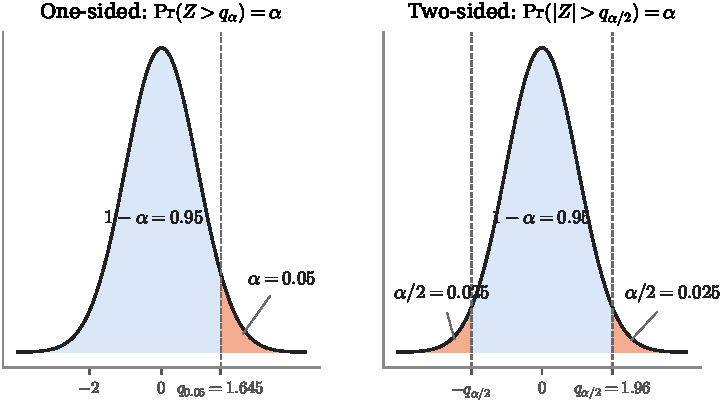
\includegraphics[width=\textwidth]{fig_gaussian_quantiles}
\caption{The standard Gaussian density with $\alpha = 0.05$. Left: the one-sided cutoff $q_{0.05} = 1.645$, with the tail of area $0.05$ in orange. Right: the two-sided cutoffs $\pm q_{0.025} = \pm 1.96$, with the two tails of area $0.025$ each in orange.}
\label{fig:gaussquantiles}
\end{figure}

Some important quantiles of the standard Gaussian, which recur so often that it is worth knowing them by heart:
\begin{center}
\begin{tabular}{@{}lcccc@{}}
\toprule
$\alpha$ & $10\%$ & $5\%$ & $2.5\%$ & $0.5\%$ \\
\midrule
$q_\alpha$ & $1.28$ & $1.645$ & $1.96$ & $2.576$ \\
\bottomrule
\end{tabular}
\end{center}
Read across: $\Pr(Z > 1.28) = 10\%$, $\Pr(Z > 1.645) = 5\%$, $\Pr(Z > 1.96) = 2.5\%$, $\Pr(Z > 2.576) = 0.5\%$.
And read two-sided: $\Pr(\abs{Z} > 1.645) = 10\%$, $\Pr(\abs{Z} > 1.96) = 5\%$, $\Pr(\abs{Z} > 2.576) = 1\%$.
The $1.96$ of every $95\%$ confidence interval is $q_{0.025}$, not $q_{0.05}$.

\begin{pitfall}[which $\alpha$ is that?]
Two conventions collide here and both are in common use.
This book's $q_\alpha$ has mass $\alpha$ \textit{above} it: $q_{0.05} = 1.645$.
Software and many textbooks index a quantile by the mass \textit{below} it: on that convention the $0.95$-quantile is $1.645$ and the $0.05$-quantile is $-1.645$.
So this book's $q_\alpha$ is the other convention's $(1 - \alpha)$-quantile, and its $q_{\alpha/2}$ for a $95\%$ interval is the other convention's $0.975$-quantile.
When a formula in this book says $q_{\alpha/2}$ and you reach for a table or software that counts from below, look up $1 - \alpha/2$.
\Cref{fig:quantiledef} is the picture to keep in mind: the subscript is the area in the upper tail.
\end{pitfall}

\begin{example}[Quantiles of the Exponential]
\label{ex:expo-quantile}
Let $X \sim \Expo(\lambda)$, with CDF $F_X(x) = 1 - e^{-\lambda x}$ for $x \geq 0$.
To find the number $x$ below which the mass is $p$, solve $F_X(x) = p$:
\begin{align*}
1 - e^{-\lambda x} &= p \\
e^{-\lambda x} &= 1 - p \\
-\lambda x &= \ln(1 - p) \\
x &= -\frac{\ln(1-p)}{\lambda}.
\end{align*}
So, for example, the 50th percentile, or median, of an Exponential r.v.\ with parameter $\lambda$ is $x = -\ln(1/2)/\lambda = \ln 2 / \lambda \approx 0.69/\lambda$, which is less than the mean $1/\lambda$ because the distribution is skewed to the right.
In this book's notation, $q_\alpha = -\ln(\alpha)/\lambda$: the subway inter-arrival time of \cref{ch:limit-tools}, with $\hat{\lambda} = 0.16$ per minute, exceeds $q_{0.05} = -\ln(0.05)/0.16 \approx 19$ minutes about one time in twenty.
\Cref{fig:expoquantile} shows the three numbers on the density.
The median, $\ln 2/\lambda = 4.3$ minutes, splits the mass in half and sits left of the mean of $1/\lambda = 6.2$ minutes because the long right tail pulls the mean up; the quantile $q_{0.05} = 18.7$ minutes leaves $5\%$ of the mass above it.
For the Gaussian the median and the mean coincide; for a skewed distribution they don't.
\end{example}

\begin{figure}[htbp]
\centering
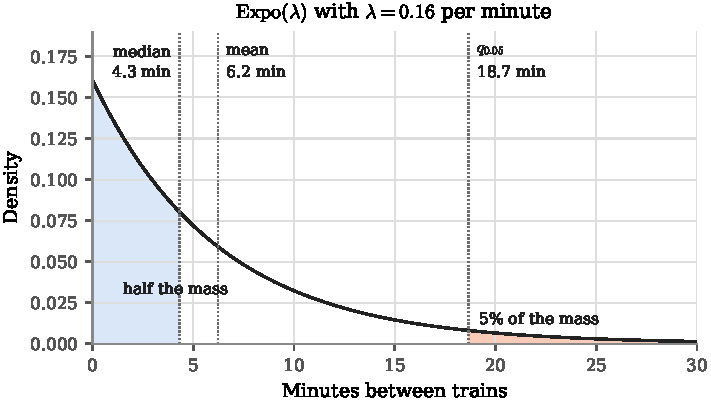
\includegraphics[width=0.8\textwidth]{fig_expo_quantile}
\caption{The $\Expo(\lambda)$ density of the subway inter-arrival times, $\lambda = 0.16$ per minute, with the median, the mean and $q_{0.05}$ marked by dotted lines. The half of the mass below the median is blue; the $5\%$ above $q_{0.05}$ is orange.}
\label{fig:expoquantile}
\end{figure}

\section{What comes next}
\label{sec:gauss-next}

This closes the probability part of the book.
Part III turns the three questions of \cref{ch:kiss} into definitions with guarantees, stated for the general model of \cref{ch:models}: \cref{ch:estimators} says what an estimator is and how to judge one; \cref{ch:confidence-intervals} and \cref{ch:tests-foundations} attach the two kinds of guarantee, an interval and a decision.
The Gaussian quantiles of this chapter appear in every formula of the last two.

\section{Summary}
\label{sec:gauss-summary}

\begin{itemize}[nosep]
\item $X \sim \Gauss(\mu, \sigma^2)$ has density $\frac{1}{\sigma\sqrt{2\pi}} \exp(-(x-\mu)^2/(2\sigma^2))$. The second parameter is the variance. The CDF has no closed form; the tails are thin enough that $3\sigma$ contains $99.7\%$ of the mass.
\item Affine transformations, in particular standardization $Z = (X - \mu)/\sigma \sim \Gauss(0,1)$, preserve Gaussianity; so do sums of independent Gaussians. The sample mean of Gaussian data is exactly $\Gauss(\mu, \sigma^2/n)$.
\item Every Gaussian probability is a table lookup after standardization: forwards for probabilities, backwards for quantiles. $\Phi(-z) = 1 - \Phi(z)$.
\item The quantile $q_\alpha$ of order $1 - \alpha$ satisfies $\Pr(X > q_\alpha) = \alpha$. For the standard Gaussian, $\Pr(\abs{Z} > q_{\alpha/2}) = \alpha$. Memorize $q_{0.05} = 1.645$ and $q_{0.025} = 1.96$, and keep straight which one a question needs.
\end{itemize}

\section{Exercises}
\label{sec:gauss-exercises}

\begin{exercise}
Let $Z \sim \Gauss(0,1)$. Compute $\Pr(Z \leq 1)$, $\Pr(Z \geq -1)$ and $\Pr(\abs{Z} > 1)$.
\end{exercise}
\begin{solution}
From the table, $\Phi(1) = 0.8413$. By symmetry $\Pr(Z \geq -1) = \Pr(Z \leq 1) = 0.8413$, and $\Pr(\abs{Z} > 1) = 2(1 - \Phi(1)) = 0.3173$. So about a third of standard Gaussian draws fall more than one standard deviation from the mean, the complement of the $68\%$ in \cref{fig:gaussdensity}.
\end{solution}

\begin{exercise}
Let $X \sim \Gauss(\mu, \sigma^2)$ and $Y = 2X$. Write down the PDF of $Y$, first from the affine property and then by the change-of-variables formula $f_Y(y) = f_X(g^{-1}(y)) / \abs{g'(g^{-1}(y))}$ for $Y = g(X)$.
\end{exercise}
\begin{solution}
By the affine property $Y \sim \Gauss(2\mu, 4\sigma^2)$, so $f_Y(y) = \frac{1}{2\sigma\sqrt{2\pi}} \exp \left( -\frac{(y - 2\mu)^2}{2 \cdot 4\sigma^2} \right)$. By change of variables with $g(x) = 2x$, $g^{-1}(y) = y/2$ and $g' = 2$: $f_Y(y) = \frac{1}{2} f_X(y/2) = \frac{1}{2\sigma\sqrt{2\pi}} \exp \left( -\frac{(y/2 - \mu)^2}{2\sigma^2} \right)$, and $(y/2 - \mu)^2 / (2\sigma^2) = (y - 2\mu)^2 / (8\sigma^2)$, the same thing.
\end{solution}

\begin{exercise}
Let $X \sim \Gauss(2, 2)$ (mean $2$, variance $2$) and let $x > 0$. Write $\Pr(X \geq -x)$ as $\Phi(g(x))$ for a function $g$ that is positive for $x > 0$.
\end{exercise}
\begin{solution}
Standardize: $(X - 2)/\sqrt{2} \sim \Gauss(0,1)$, so $\Pr(X \geq -x) = \Pr \left( Z \geq \frac{-x - 2}{\sqrt{2}} \right) = 1 - \Phi \left( -\frac{x+2}{\sqrt{2}} \right) = \Phi \left( \frac{x + 2}{\sqrt{2}} \right)$ by symmetry. For $x = 1$ this is $\Phi(2.12) = 0.983$.
\end{solution}

\begin{exercise}
Verify the three numbers of the empirical rule from a table, and find $\Pr(\abs{X - \mu} > 2\sigma)$ for any Gaussian $X$. Why doesn't the answer depend on $\mu$ or $\sigma$?
\end{exercise}
\begin{solution}
$2\Phi(1) - 1 = 0.6827$, $2\Phi(2) - 1 = 0.9545$, $2\Phi(3) - 1 = 0.9973$. The complement of the second is $\Pr(\abs{X - \mu} > 2\sigma) = \Pr(\abs{Z} > 2) = 0.0455$. The event $\abs{X - \mu} > 2\sigma$ is the event $\abs{Z} > 2$ for the standardized variable, whose distribution is the same whatever $\mu$ and $\sigma$ are.
\end{solution}

\begin{exercise}
For $\alpha = 0.10$, what is the cutoff $c$ such that $\Pr(Z > c) = 0.10$, and what is the cutoff $c'$ such that $\Pr(\abs{Z} > c') = 0.10$? Which of the two belongs in a $90\%$ confidence interval of the form $\bar{X}_n \pm c \, \sigma / \sqrt{n}$?
\end{exercise}
\begin{solution}
$c = q_{0.10} = 1.28$ and $c' = q_{0.05} = 1.645$. A confidence interval is a two-sided statement (the truth may be on either side of the estimate), so it needs $c' = 1.645$: $\Pr(\abs{\bar{X}_n - \mu} \leq 1.645 \, \sigma/\sqrt{n}) \approx 0.90$. Using $1.28$ would give an $80\%$ interval.
\end{solution}


\partintro{The three questions of \cref{ch:kiss} become definitions with guarantees, stated for the general model of \cref{ch:models} and computed for the kiss experiment. An estimator (\cref{ch:estimators}) is a guess inside the model, judged by bias, variance and risk; a confidence interval (\cref{ch:confidence-intervals}) and a test (\cref{ch:tests-foundations}) are the two ways of attaching a guarantee to the guess.}
\part{Foundations of Inference}
\chapter{Estimators: Bias, Variance and Risk}
\label{ch:estimators}

\begin{chaptergoals}
\begin{itemize}[nosep]
\item What a statistic is, what an estimator is, and the sense in which a statistic throws information away (and when, by the sufficiency principle, that's fine).
\item The two large-sample properties an estimator should have: consistency (it gets to the truth) and asymptotic normality (it gets there at rate $1/\sqrt{n}$ with a Gaussian error), and why the asymptotic variance is not the limit of the variance.
\item The two finite-sample measures: bias and variance, with Jensen's inequality as the reason transformed estimators pick up bias.
\item Quadratic risk $=$ variance $+$ bias$^2$, and the trade-off it makes visible: a biased estimator can beat an unbiased one, and no estimator wins for every value of the parameter.
\end{itemize}
The running example is again the kiss experiment, $R_1, \ldots, R_n \iid \Bern(p)$ with $n = 124$, now with several competing estimators of $p$.
\Cref{ch:models} fixed the object inside which inference happens, and Part II supplied the three limit facts about averages; the first task inside the model is to guess $\theta$ from the data, and this chapter says what a guess is and how to judge one.
\end{chaptergoals}

\section{Statistics and estimators}
\label{sec:est-statistics}

\begin{definition}[Statistic, estimator]
\label{def:estimator}
A \textbf{statistic} is any measurable function of the sample: $T = T(\Xton)$.
For example, $\bar{X}_n$, $\max_i X_i$, $X_1 + \log(1 + \abs{X_n})$, the sample variance, and so on.
As a statistic is a function of your data, it's an r.v.

An \textbf{estimator} of $\theta$ is a statistic $\ethn = \ethn(\Xton)$ whose expression doesn't depend on $\theta$.
\end{definition}

\begin{inwords}
\textbf{In words.} A statistic is anything you can compute from the data. An estimator is a statistic you intend as a guess for $\theta$, and its formula may use the data and known constants only, never $\theta$.
\par\smallskip
\textbf{For the kiss data.} $\bar{R}_n$ is a statistic and an estimator of $p$. $\bar{R}_n - p$ is a random variable but not a statistic, since you cannot compute it. $\max_i R_i$ is a statistic (it is $1$ unless every couple turned left) and a useless estimator of $p$.
\end{inwords}

The word `measurable' is a technicality from probability theory \toolkit{sec:math-rv}; the working rule of thumb is that if you can compute it exactly once you're given the data, it's measurable.
Things that are only implicitly defined, such as a $\sup$ or $\inf$ over an infinite family \toolkit{sec:math-sup}, can fail the condition, but every statistic this book writes down is a formula in the observations and passes it.

The clause `doesn't depend on $\theta$' is the whole content of the second definition.
$\bar{R}_n$ is an estimator of $p$ in the kiss model; $\bar{R}_n - p$ is neither a statistic nor an estimator because you can't compute it from the data alone: its formula involves the thing you're trying to estimate. (It is a perfectly good random variable, and it has a name, the \textbf{estimation error}, which is the quantity the rest of this chapter measures.)
The constant $0.5$ is an estimator of $p$ (a bad one, as \cref{sec:est-strengths} will show), and so is $X_1$: the definition says what an estimator is, not what a good one is.
The rest of the chapter is about telling them apart.

Recall from \cref{ch:kiss} the distinction between an estimator and an estimate: the estimator $\ethn$ is a random variable, with a distribution, an expectation and a variance; the \textit{estimate} $\hat{\theta}_n(x_1, \ldots, x_n)$ is the number it produces on your one sample.
Every property defined in this chapter is a property of the random variable.

\section{A statistic reduces the data}
\label{sec:est-reduction}

Let $\matx = (\Xton)$ be the vector of observations and $\vecx = (x_1, \ldots, x_n)$ a realized sample.
Any statistic $T(\matx)$ defines a form of data reduction.
Anyone who uses only the observed value of the statistic, $T(\vecx)$, rather than the entire observed sample $\vecx$, will treat as equal two samples, $\vecx$ and $\vecy$, that satisfy $T(\vecx) = T(\vecy)$ even though the actual sample values may differ.

Data reduction in terms of a particular statistic can be thought of as a partition of the sample space $E^n$.
For illustration, suppose a sample of size $n$ is drawn and $\bar{x} = 8$.
There are many points in $E^n$ which have the same mean of $8$, and you can think of them as belonging to the set $\{ (x_1, \ldots, x_n) : \bar{x} = 8 \}$.
In fact, all points on the hyperplane
\[
x_1 + \cdots + x_n = 8n
\]
yield the mean $\bar{x} = 8$, and thus the hyperplane is the set.
But there are of course many values that $\bar{X}_n$ can take, and thus there are many such sets.
In this sense, the sample mean, or any statistic, partitions the sample space into a collection of sets (equivalence classes).
\Cref{fig:partition} draws this for $n = 2$, where the sample space is the plane and the hyperplanes are lines, next to the quite different partition induced by the maximum.
On the left, the samples $(1.5, 4.5)$ and $(4.5, 1.5)$ lie on the same line and are the same sample to anyone who only sees $\bar{x} = 3$.
On the right, the level sets of the maximum are L-shapes, and $(1.5, 4.5)$ and $(4.5, 4.5)$ are the same sample to anyone who only sees $\max = 4.5$.
Each statistic keeps one number and discards the rest, and which rest is discarded depends on the statistic.

\begin{figure}[htbp]
\centering
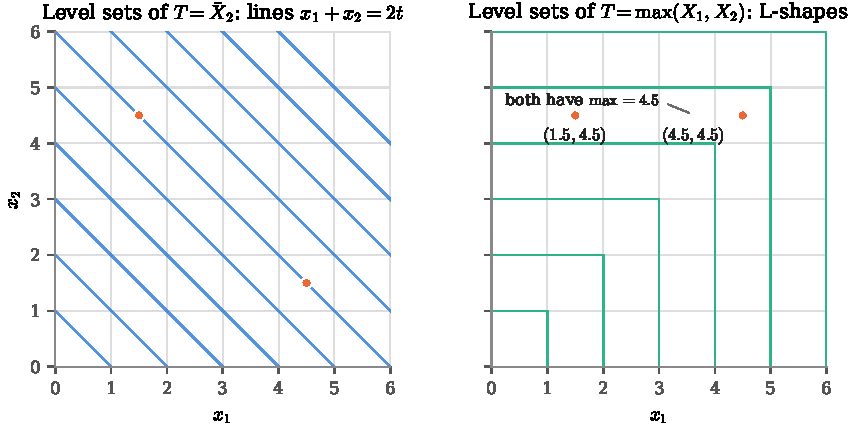
\includegraphics[width=\textwidth]{fig_statistic_partition}
\caption{Level sets of the sample mean (left, the lines $x_1 + x_2 = 2t$) and of the maximum (right, L-shapes) for a sample of size $n = 2$, a point in the plane. Orange dots mark two samples on one level set.}
\label{fig:partition}
\end{figure}

Let $\mathcal{T} = \{ t = T(\vecx) \text{ for some } \vecx \in E^n \}$ be the image of $E^n$ under $T$;
that is, $\mathcal{T}$ is the set of all possible values of the statistic.
Then $T$ partitions the sample space into the sets $A_t = \{ \vecx : T(\vecx) = t \}$ for $t \in \mathcal{T}$.
Samples $\vecx_1$ and $\vecx_2$ belong to the same set if and only if $T(\vecx_1) = T(\vecx_2)$.
The statistic summarizes the data in that, rather than reporting the entire sample $\vecx$, it reports only that $T(\vecx) = t$ or, equivalently, $\vecx \in A_t$.

\subsection{The sufficiency principle}

A \textbf{sufficient statistic} for a parameter $\theta$ is a statistic that, in a certain sense, captures all the information about $\theta$ contained in the sample.
Any additional information in the sample, besides the value of the sufficient statistic, does not contain any more information about $\theta$.
This leads to the data reduction technique called the sufficiency principle.

\textbf{Sufficiency principle:} If $T(\matx)$ is a sufficient statistic for $\theta$, then any inference about $\theta$ should depend on the sample $\matx$ only through the value $T(\matx)$.
That is, if $\vecx$ and $\vecy$ are two sample points such that $T(\vecx) = T(\vecy)$, then the inference about $\theta$ should be the same whether $\matx = \vecx$ or $\matx = \vecy$ is observed.

\begin{definition}[Sufficient statistic]
\label{def:sufficient}
A statistic $T(\matx)$ is a \textbf{sufficient statistic for} $\theta$ if the conditional distribution of the sample $\matx$ given the value of $T(\matx)$ does not depend on $\theta$.
\end{definition}

\begin{inwords}
\textbf{In words.} Once you know the value of $T$, the rest of the sample looks the same whatever $\theta$ is, so the rest carries no further information about $\theta$.
\par\smallskip
\textbf{For the kiss data.} Given that $80$ of $124$ couples turned right, every ordering of the $80$ ones and $44$ zeros is equally likely, whatever $p$ is; the count is sufficient and the order tells you nothing more about $p$. The example below does the computation.
\end{inwords}

\begin{example}
\label{ex:sufficient-bernoulli}
In the kiss model, the number of couples turning right $S = \sum_i R_i$ is sufficient for $p$.
Given $S = s$, every arrangement of $s$ ones and $n - s$ zeros is equally likely:
\[
\Pr_p(\matx = \vecx \mid S = s) = \frac{p^s (1-p)^{n-s}}{\binom{n}{s} p^s (1-p)^{n-s}} = \frac{1}{\binom{n}{s}},
\]
which doesn't involve $p$.
Once you know $80$ of $124$ couples turned right, the order in which they did so tells you nothing further about $p$.
This is why every method in this book for this model is a function of $\bar{R}_n$ alone: by the sufficiency principle, nothing else in the sample tells you more about $p$, if the model is right. (The order of the $R_i$ is exactly what you would look at to check whether it is, as with the wedding reception of exercise 4(b) in \cref{ch:kiss}, whose couples would show up as a run of $1$s.)
\end{example}

Sufficiency has a large theory of its own, which this book does not take up; it appears once more, in \cref{ch:exp-families}, where the exponential families make the sufficient statistic visible.
It is here because it says precisely what the data reduction in \cref{fig:partition} is allowed to throw away: everything except $T$, whenever the conditional distribution of the sample given $T$ is free of $\theta$.

\section{Consistency}
\label{sec:est-consistency}

The best estimator would be the one that equals the parameter of interest.
Given the probabilistic nature of statistics, ascertaining rules to derive such an estimator is hopeless.
But there are desirable properties you want estimators to have.

For example, as you collect more and more data you should get a better and better idea of which distribution generated the data.
In the limit, as your sample size increases to infinity you should know exactly which distribution it is.
Specifically, you want an estimator that converges to the true parameter $\theta$ as your sample size goes to infinity.
An estimator satisfying this property is called \textit{consistent}, and it comes in two forms, depending on whether the convergence is in probability or almost surely.

\begin{definition}[Consistency]
\label{def:consistent}
An estimator $\ethn$ of $\theta$ is \textbf{weakly consistent} if
\[
\ethn \convp \theta \quad (\text{with respect to } \Pr_\theta),
\]
that is, $\Pr_\theta \left( \abs{\ethn - \theta} \geq \epsilon \right) \to 0$ for every $\epsilon > 0$, and \textbf{strongly consistent} if $\ethn \convas \theta$ (almost sure convergence is defined in \cref{app:modes}; the unqualified word `consistent' is used for either, in this book and in common usage).
Here $\Pr_\theta$ is the distribution that generated the data, and the statement is required to hold for every $\theta \in \Theta$.
\end{definition}

\begin{inwords}
\textbf{In words.} With enough data the estimator lands as close to the truth as you like, with probability as high as you like, and this must be so whichever value the truth has.
\par\smallskip
\textbf{For the kiss data.} $\bar{R}_n \convp p$ is the Law of Large Numbers, so $\bar{R}_n$ is consistent. The constant estimator $0.5$ is not: it never moves, so it only gets close to $p$ if $p$ happens to be $0.5$, and consistency has to hold for every $p$.
\end{inwords}

The Law of Large Numbers is the consistency of $\bar{X}_n$ for $\mu$; its weak form (\cref{thm:wlln}) gives weak consistency, its strong form (\cref{thm:slln} in \cref{app:modes}) strong consistency.
\recall{The Law of Large Numbers says that an average of independent draws settles on the number it is an average of: for any width you name, the probability that $\bar{X}_n$ sits outside a band of that width around $\mu$ goes to zero. It says nothing about how fast, and nothing about the shape of what is left; those are the Central Limit Theorem's business.}
The continuous mapping theorem (\cref{ch:limit-tools}) then makes any continuous function of a consistent estimator consistent for the corresponding function of the parameter.
\recall{The continuous mapping theorem says that applying a continuous function to a converging sequence gives a converging sequence, with the function applied to the limit: if $\hat\theta_n \convp \theta$ and $g$ is continuous at $\theta$, then $g(\hat\theta_n) \convp g(\theta)$. It is the rule that lets you take square roots and reciprocals of estimators without starting over.}

Consistency only takes a stand on where the distribution of $\ethn$ \textit{concentrates}, not on the whole distribution.
This is evident from its definition; consistency is defined in terms of convergence in probability or almost surely, and both are statements about the limit being a point.
But consistency usually isn't enough to do inference because you want to know not just where the estimator concentrates but also the precision with which it concentrates, and how fast.

\begin{example}[How fast is consistent?]
\label{ex:rate}
Let $\Xton \iid \Bern(p)$.
What is the smallest $c$ such that $n^c(\bar{X}_n - p)$ does \textit{not} converge to $0$ in probability?
By the CLT, $\sqrt{n}(\bar{X}_n - p)/\sigma \convd \Gauss(0,1)$ with $\sigma = \sqrt{p(1-p)}$, so for $c < 1/2$,
\[
n^c (\bar{X}_n - p) = \frac{\sigma}{n^{1/2 - c}} \cdot \frac{\sqrt{n}}{\sigma} (\bar{X}_n - p) \convd 0 \cdot \Gauss(0,1) = 0
\]
by Slutsky, which is convergence in probability to $0$ since the limit is a constant.
At $c = 1/2$ the limit is $\Gauss(0, \sigma^2)$, not $0$.
So $c = 1/2$: the estimation error $\bar{X}_n - p$ is of exact order $1/\sqrt{n}$, and such an estimator is called \textit{$\sqrt{n}$-consistent}.
That is more than consistency says, and it's the second property.
\end{example}

\section{Asymptotic normality}
\label{sec:est-asymptotic-normality}

This is where the property of asymptotic normality enters, which unlike consistency is \textit{defined in terms of convergence in distribution}.
Asymptotic normality is a property of an estimator that, if present, gives it CLT-like behavior: a Gaussian limiting distribution.
Unlike the CLT, it's not a theorem; it's a property that a given estimator may or may not have, and specifically a property of estimators, hence concerned with inference.
For reasons addressed below, it involves some scaling in order to circumvent a problem with the variance of the limiting distribution.

\begin{definition}[Asymptotic normality]
\label{def:asymp-normal}
An estimator $\ethn$ of $\theta$ is \textbf{asymptotically normal} if
\[
\sqrt{n}(\ethn - \theta) \convd \Gauss(0, \sigma^2).
\]
The variance of this limiting distribution, $\sigma^2$, is called the \textbf{asymptotic variance} of $\ethn$.
\end{definition}

\begin{inwords}
\textbf{In words.} Magnify the estimation error by $\sqrt{n}$ and it settles into a bell curve centered at $0$. Unmagnified, the error is approximately $\Gauss(0, \sigma^2/n)$: shrinking like $1/\sqrt{n}$, with a known shape.
\par\smallskip
\textbf{For the kiss data.} $\sqrt{n}(\bar{R}_n - p) \convd \Gauss(0, p(1-p))$ by the CLT, so $\bar{R}_n$ is asymptotically normal with asymptotic variance $p(1-p) = 0.229$ at $p = 0.645$, and its error at $n = 124$ is approximately $\Gauss(0, 0.043^2)$.
\end{inwords}

\textbf{NB$_1$:} You might imagine the `natural' form of the asymptotic variance would simply be the limit of $\var(\ethn)$ as $n$ goes to infinity.
\textbf{This is not what it is.}
Why not?
Think about the estimator $\bar{X}_n$.
Its variance is $\var(\bar{X}_n) = \sigma^2/n$, and hence, as $n \to \infty$, it converges to 0.
It'd be silly to let `asymptotic variance' refer to something that's always 0.
Hence, the asymptotic variance $\sigma^2$ is \textit{not} the limit of the variance of $\ethn$.
\Cref{fig:asympvar} shows the two quantities side by side for the kiss estimator.
On the left, $\var(\hat{p}) = p(1-p)/n$ goes to zero, and its limit carries no information about precision.
On the right, $n \cdot \var(\hat{p}) = p(1-p) = 0.229$ is constant, and that constant is the asymptotic variance, the variance of the limiting Gaussian of $\sqrt{n}(\hat{p} - p)$.

\begin{figure}[htbp]
\centering
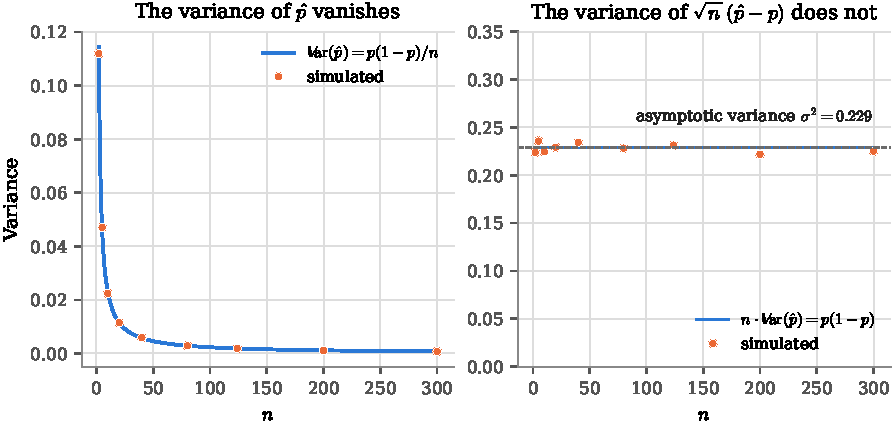
\includegraphics[width=\textwidth]{fig_asymptotic_variance}
\caption{For $\hat{p} = \bar{R}_n$ with $p = 0.645$, against $n$. Left: $\var(\hat{p}) = p(1-p)/n$. Right: $n \cdot \var(\hat{p})$, with the asymptotic variance as a gray dashed line. Blue curves are exact; orange dots are variances estimated from $4{,}000$ simulated samples at each $n$.}
\label{fig:asympvar}
\end{figure}

\textbf{NB$_2$:} This brings us to the rescaling in the definition of asymptotic normality.
The rescaling by $\sqrt{n}$ is crucial because it holds the \textit{spread} of the error fixed as the sample size increases, which is what allows a non-degenerate Gaussian limit to exist at all.
To understand why, again think about $\bar{X}_n$: without the rescaling, $\bar{X}_n - \mu$ converges to the degenerate distribution at $0$, which is consistency restated and says nothing about precision.
With it, $\sqrt{n}(\bar{X}_n - \mu)$ has variance $\sigma^2$ for every $n$ and a Gaussian limit.
For the sample mean the asymptotic variance therefore coincides with $n \var(\bar{X}_n)$; in general it is defined as the variance of the limiting Gaussian, which is the only definition that always makes sense, since convergence in distribution does not by itself say anything about variances.
This is the two-scales picture of \cref{sec:conv-two-scales}, and \cref{ex:rate} says why $\sqrt{n}$ and not some other power.

\textbf{NB$_3$:} Note also that you subtract the unknown parameter $\theta$ from $\ethn$ in the definition.
This focuses attention on the deviation of the estimator from its true value, $\ethn - \theta$, which is the estimation error, the quantity you actually care about.

\begin{intuition}[what asymptotic normality buys]
For large $n$ the error of an asymptotically normal estimator is approximately $\Gauss(0, \sigma^2/n)$.
That one sentence gives you a standard error, $\sigma/\sqrt{n}$; an error bar, $\ethn \pm 1.96 \sigma/\sqrt{n}$ with probability about $95\%$; and a test of any hypothesis about $\theta$.
Consistency says the error vanishes; asymptotic normality says how big it is at the $n$ you have and what shape it has.
\Cref{ch:confidence-intervals} is entirely about using the sentence.
When the asymptotic variance depends on $\theta$ (as $p(1-p)$ does), you'll replace it by a consistent estimate and lean on Slutsky, as in \cref{ch:limit-tools}.
\end{intuition}

\section{Bias}
\label{sec:est-bias}

Consistency and asymptotic normality are properties of the limit.
The next two are properties of $\ethn$ at the sample size you actually have.

\begin{definition}[Bias]
\label{def:bias}
The \textbf{bias} of an estimator $\ethn$ of $\theta$ is
\[
\Bias(\ethn) = \E_\theta[\ethn] - \theta.
\]
If $\Bias(\ethn) = 0$ for every $\theta \in \Theta$, the estimator is called \textbf{unbiased}.
\end{definition}

\begin{inwords}
\textbf{In words.} Average the estimator over all the samples you could have drawn; the bias is how far that average sits from the truth.
\par\smallskip
\textbf{For the kiss data.} $\E[\bar{R}_n] = p$, so $\bar{R}_n$ is unbiased; the constant $0.5$ has bias $0.5 - p$, which is $-0.145$ if $p = 0.645$.
\end{inwords}

An unbiased estimator is right on average: if you could repeat the experiment many times, the estimates would be scattered around $\theta$ with no systematic lean.
It says nothing about how widely they're scattered.

\begin{worked}[four estimators of $p$: bias]
Let $\Xton \iid \Bern(p)$ and consider four candidate estimators of $p$, the first three of which look respectable and the fourth of which does not.
\begin{enumerate}[nosep]
\item $\hat{p} = \bar{X}_n$: $\E[\bar{X}_n] = p$, so the bias is $0$.
\item $\hat{p} = X_1$: $\E[X_1] = p$, bias $0$. Unbiased, and it ignores $n - 1$ observations.
\item $\hat{p} = (X_1 + X_2)/2$: $\E = p$, bias $0$.
\item $\hat{p} = \sqrt{\ind(X_1 = 1, X_2 = 1)}$: the indicator is $1$ with probability $p^2$, and the square root of $0$ or $1$ is itself, so $\E[\hat{p}] = p^2$ and the bias is $p^2 - p = -p(1-p) < 0$.
This estimator is systematically too low.
\end{enumerate}
The fourth one is a trap for anyone who moves a square root through an expectation: $\sqrt{\E[\cdot]}$ is not $\E[\sqrt{\cdot}]$.
\end{worked}

\begin{worked}[a biased sample mean]
Let $\Xton \iid \text{Unif}([a, a+1])$ with $a$ unknown.
Then $\E[\bar{X}_n] = \E[X_1] = \int_a^{a+1} x \, \mathrm{d}x = a + \frac12$, so $\bar{X}_n$ has bias $\frac12$ as an estimator of $a$, for every $n$: more data doesn't help because the lean is built in.
The fix is obvious once the bias is known: $\bar{X}_n - \frac12$ is unbiased for $a$.
A known bias that doesn't depend on the unknown parameter is as good as no bias at all; the dangerous biases are the ones you don't know, and the awkward ones are those that depend on the parameter, like the subway bias below.
\end{worked}

\subsection{Jensen's inequality}

The fourth estimator above is a case of a general fact: applying a convex (or concave) function to an unbiased estimator produces a biased one, and the direction of the bias is predictable.

A function $g: \real \to \real$ is \textbf{convex} if for all $x_1 < x_2$ and all $0 \leq t \leq 1$,
\[
g(t x_1 + (1 - t) x_2) \leq t g(x_1) + (1 - t) g(x_2):
\]
the graph of $g$ lies below every chord.
Now read the right-hand side probabilistically.
Let $X$ take the value $x_1$ with probability $t$ and $x_2$ with probability $1 - t$.
Then $t x_1 + (1-t) x_2 = \E[X]$ and $t g(x_1) + (1-t) g(x_2) = \E[g(X)]$, so convexity says $g(\E[X]) \leq \E[g(X)]$ for every two-point $X$.
It holds in general.

\begin{theorem}[Jensen's inequality]
\label{thm:jensen}
For any r.v.\ $X$ with finite mean and any convex function $g$,
\[
g(\E[X]) \leq \E[g(X)].
\]
For a concave $g$ the inequality reverses.
\end{theorem}
The two-point argument above is the whole idea; the general case replaces the chord by the tangent line at $\E[X]$, which for a convex $g$ lies below the curve everywhere \toolkit{sec:math-convex}; evaluating that line at $X$ and taking expectations kills its linear term and leaves exactly $g(\E[X]) \leq \E[g(X)]$.

\Cref{fig:jensen} draws the two-point case for $g(x) = 1/x$ and an $X$ equal to $1$ or $4$ with probability $\frac12$ each.
The point $(\E[X], \E[g(X)])$ is the midpoint of the chord, and the chord lies above the curve, so $\E[g(X)] = 0.625$ exceeds $g(\E[X]) = 0.4$.
For any convex $g$, averaging first and transforming second gives less than transforming first and averaging second.

\begin{figure}[htbp]
\centering
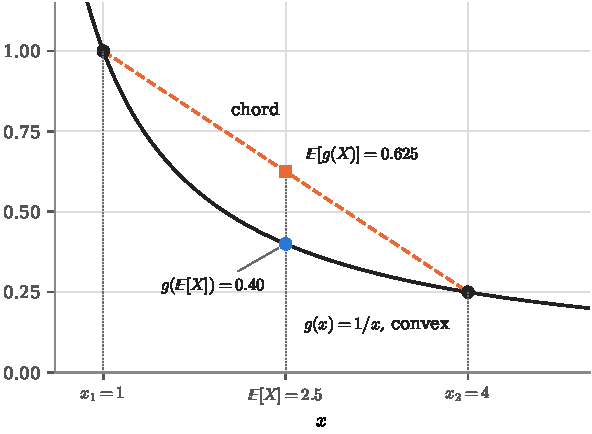
\includegraphics[width=0.7\textwidth]{fig_jensen}
\caption{Jensen's inequality for $g(x) = 1/x$ (solid curve) and an $X$ equal to $1$ or $4$ with probability $\frac12$ each. The orange dashed line is the chord; the blue dot is $(\E[X], g(\E[X]))$ and the orange square is $(\E[X], \E[g(X)])$.}
\label{fig:jensen}
\end{figure}

\begin{example}[The subway rate again]
In \cref{ch:limit-tools} the rate of the T was estimated by $\hat{\lambda} = 1/\bar{T}_n$, with $\E[\bar{T}_n] = 1/\lambda$.
Since $g(x) = 1/x$ is convex on $(0, \infty)$, Jensen gives $\E[1/\bar{T}_n] \geq 1/\E[\bar{T}_n] = \lambda$: the estimator is biased upward, for every $n$.
The bias does vanish as $n$ grows, but not because the estimator is consistent and asymptotically normal (neither property says anything about the bias); it vanishes because an exact computation gives $\E[1/\bar{T}_n] = \frac{n}{n-1}\lambda$, a bias of $\lambda/(n-1)$, which is of order $1/n$ and so is swamped by the $1/\sqrt{n}$ standard error. The exercises take this up.
Biased and consistent is a common combination, and nothing is wrong with it.
\end{example}

\begin{bridge}[why the sample variance divides by $n - 1$]
An introductory course divides the sum of squared deviations by $n - 1$, and the reason is a bias calculation.
For $\Xton$ i.i.d.\ with mean $\mu$ and variance $\sigma^2$, the natural estimator $\frac{1}{n} \sum (X_i - \bar{X}_n)^2$ has expectation
\[
\E \left[ \frac1n \sum_{i=1}^n (X_i - \bar{X}_n)^2 \right] = \E \left[ \frac1n \sum_{i=1}^n (X_i - \mu)^2 \right] - \E \left[ (\bar{X}_n - \mu)^2 \right] = \sigma^2 - \frac{\sigma^2}{n} = \frac{n-1}{n} \sigma^2,
\]
using $\sum (X_i - \bar{X}_n)^2 = \sum (X_i - \mu)^2 - n(\bar{X}_n - \mu)^2$.
Its bias is $-\sigma^2/n$: the deviations from $\bar{X}_n$ are systematically smaller than the deviations from $\mu$ because $\bar{X}_n$ was chosen to be in the middle of this sample.
Multiplying by $n/(n-1)$ removes the bias exactly, which is the $S^2 = \frac{1}{n-1} \sum (X_i - \bar{X}_n)^2$ you were taught.
Both versions are consistent; the correction matters at $n = 5$ and not at $n = 500$.
\end{bridge}

\section{Variance}
\label{sec:est-variance}

An estimator is a random variable, so it has a variance, $\var(\ethn) = \E[(\ethn - \E[\ethn])^2]$, which measures how widely it scatters around its own mean (not around $\theta$).
Small variance means the estimate you got is close to the estimate you would have got from a different sample; it says nothing about whether either is close to $\theta$.

\begin{worked}[four estimators of $p$: variance]
For the same four estimators, with $\var(X_i) = p(1-p)$:
\begin{enumerate}[nosep]
\item $\bar{X}_n$: $\var = p(1-p)/n$, since the variance of a sum of independent terms is the sum of the variances.
\item $X_1$: $\var = p(1-p)$. Unbiased, but as variable as a single coin flip, however large $n$ is.
\item $(X_1 + X_2)/2$: $\var = p(1-p)/2$.
\item $\sqrt{\ind(X_1 = 1, X_2 = 1)}$: a Bernoulli with parameter $p^2$, so $\var = p^2(1 - p^2)$.
\end{enumerate}
The first three are unbiased, so among them the comparison is purely on variance, and $\bar{X}_n$ wins by a factor of $n$ over $X_1$.
This is the sense in which using all the data matters: an unbiased estimator that ignores observations is paying in variance for no return in bias.
\Cref{fig:fourestimators} draws all four sampling distributions on one axis.
$\bar{X}_n$ is a narrow spike at $p$.
$X_1$ is two bars, at $0$ and $1$: unbiased, since its mean is $p$, and never anywhere near $p$.
$(X_1 + X_2)/2$ is three bars.
The square-root indicator is two bars with its mean at $p^2 = 0.42$, off the truth.
Bias is where the triangle sits relative to the orange line, variance is how spread out the bars are, and only the first estimator does well on both.
\end{worked}

\begin{figure}[htbp]
\centering
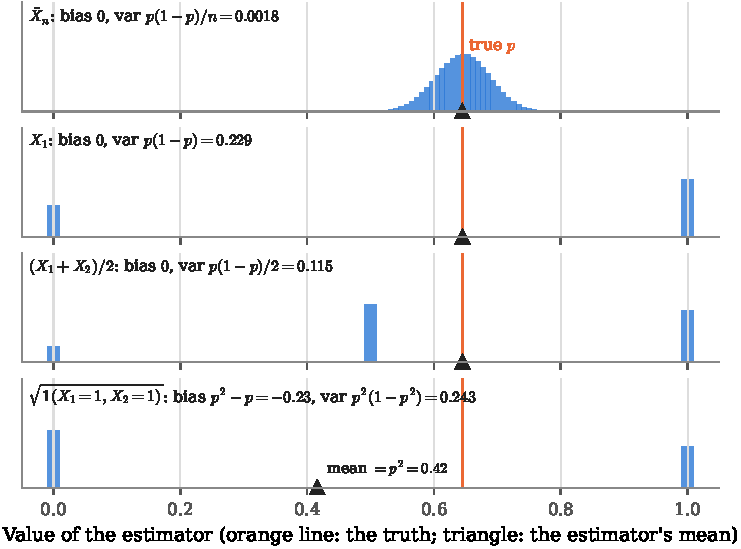
\includegraphics[width=\textwidth]{fig_four_estimators}
\caption{The exact sampling distributions (blue bars) of the four estimators of $p$ at $n = 124$, $p = 0.645$. The orange line is the true $p$; the black triangle under each axis is the estimator's mean.}
\label{fig:fourestimators}
\end{figure}

For the uniform example, $\var(\bar{X}_n) = \var(X_1)/n = \frac{1}{12n}$, and the bias-corrected $\bar{X}_n - \frac12$ has the same variance, since subtracting a constant changes nothing.

\section{Quadratic risk}
\label{sec:est-risk}

It may not be possible to find an estimator that is both unbiased and has the smallest variance.
Is there a compromise that can be made between a biased estimator and a high-variance one?
That is, can you find an estimator that simply has a small bias and a small variance?
That's where the quadratic risk comes in: a single number that charges for both.

\begin{definition}[Quadratic risk]
\label{def:risk}
The \textbf{quadratic risk} (or \textbf{risk}) of an estimator $\ethn \in \real$ is
\[
R(\ethn) = \E_\theta \left[ \abs{\ethn - \theta}^2 \right],
\]
the expected squared distance from the estimator to the truth.
It is more commonly called the \textbf{mean squared error}, and the two names mean the same thing.
\end{definition}

\begin{inwords}
\textbf{In words.} Square the miss, average over all possible samples. One number that punishes both a systematic lean and a wide scatter.
\par\smallskip
\textbf{For the kiss data.} $R(\bar{R}_n) = p(1-p)/n = 0.00185$ at $p = 0.645$, $n = 124$; a typical miss is its square root, $0.043$.
\end{inwords}

\begin{theorem}[Bias-variance decomposition]
\label{thm:bias-variance}
\[
R(\ethn) = \var(\ethn) + \Bias(\ethn)^2.
\]
\end{theorem}

\coreproof{Add and subtract $\E[\ethn]$ inside the square, expand, and watch the cross term vanish because $\E[\ethn - \E[\ethn]] = 0$.}
\begin{proof}
First note that $\abs{\ethn - \theta}^2 = (\ethn - \theta)^2$.
Add and subtract $\E[\ethn]$ inside the square and expand:
\begin{align*}
R(\ethn) &= \E\left[ ( \ethn - \E[\ethn] + \E[\ethn] - \theta)^2 \right] \\
	&= \E \left[ (\ethn  - \E[\ethn])^2 \right] + \E \left[ (\E[\ethn] - \theta)^2 \right] + 2 \E\left[(\ethn - \E[\ethn]) (\E[\ethn] - \theta) \right] \\
	&= \var(\ethn) + (\E[\ethn] - \theta)^2 + 2 (\E[\ethn] - \theta) \, \E\left[\ethn - \E[\ethn] \right] \\
	&= \var(\ethn) + \Bias(\ethn)^2 + 2 (\E[\ethn] - \theta) \cdot 0.
\end{align*}
In the second term, $\E[\ethn] - \theta$ is a number, so its expectation is itself; in the third, the same number comes out of the expectation, and what remains, $\E[\ethn - \E[\ethn]]$, is zero.
\end{proof}

\begin{bridge}[the MSE in an ANOVA table]
An introductory course's ANOVA table reports MSE, the mean square for error: the squared deviations of the observations from their group means, summed and divided by $N - k$ for $N$ observations in $k$ groups (simple regression output divides the sum of squared residuals by $N - 2$ instead).
It shares a name with the quadratic risk, but the squares it averages are residuals, not an estimator's misses.
MSE is a statistic, computed from the data, and an unbiased estimator of $\sigma^2$, the common variance of the model's errors.
The quadratic risk is an expectation under $\Pr_\theta$, a function of the unknown parameter, and no data set produces it.
The two meet in the standard error: with one group the MSE is the sample variance $S^2$, and $S^2/n$, the square of the estimated standard error $S/\sqrt{n}$, is an unbiased estimator of $\sigma^2/n$, which is the risk of $\bar{X}_n$ since $\bar{X}_n$ is unbiased.
\end{bridge}

The decomposition is the reason a biased estimator can be the better one: if accepting a little bias buys a large reduction in variance, the risk goes down.
It also makes a point that is easy to miss when you only ever compute bias and variance separately: the risk is a function of $\theta$, through both terms, and an estimator that is best for one value of $\theta$ need not be best for another.
\Cref{fig:biasvariance} shows both facts in the kiss model.
On the left, at $p = 0.645$ and $n = 124$, $\bar{R}_n$ is unbiased with standard deviation $0.043$.
The shrinkage estimator $(n\bar{R}_n + 10)/(n + 20)$ pulls the estimate toward $\frac12$, as if $20$ extra coin flips had come up half heads; it is biased by $-0.020$ but has standard deviation $0.037$, and its risk, $0.00177$, is smaller than $\bar{R}_n$'s $0.00185$.
On the right, the risk of four estimators is plotted against the true $p$.
Shrinkage beats $\bar{R}_n$ for $p$ between $0.34$ and $0.66$ and loses outside; the constant $0.5$ is unbeatable at $p = 0.5$ and terrible elsewhere; $X_1$ is unbiased and hopeless everywhere.
No curve lies below all the others, so `best estimator' is not a well-posed question without saying for which $p$.

\begin{figure}[htbp]
\centering
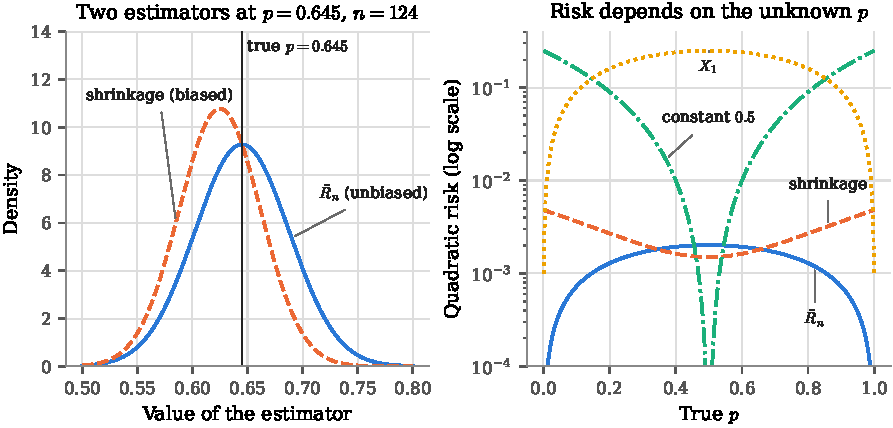
\includegraphics[width=\textwidth]{fig_bias_variance}
\caption{The kiss model, $n = 124$. Left: Gaussian approximations to the sampling distributions of $\bar{R}_n$ (solid) and the shrinkage estimator (dashed) at $p = 0.645$. Right: risk against the true $p$, log scale: $\bar{R}_n$ (solid), shrinkage (dashed), the constant $0.5$ (dash-dot), $X_1$ (dotted).}
\label{fig:biasvariance}
\end{figure}

\begin{intuition}[bias and variance as a target]
Think of the truth $\theta$ as the bull's-eye and each estimate as a shot.
Variance is how tight the group is; bias is how far the center of the group is from the bull's-eye.
The risk is the average squared distance of a shot from the bull's-eye, and the decomposition says it's the squared distance of the group's center plus the group's spread: a tight group off to one side can be closer on average than a loose group centered on the target.
The shrinkage estimator in \cref{fig:biasvariance} is the tight group off to one side.
What the target picture doesn't show is that moving the bull's-eye (changing $p$) changes which group is closer, and that's the right of \cref{fig:biasvariance}.
\Cref{fig:target} draws the four combinations.
The cross in each is $\E[\ethn]$, so bias is the distance from the cross to the bull's-eye, variance is the spread of the dots around the cross, and the risk is the average squared distance from a dot to the bull's-eye, which the decomposition splits into the two.
Lower left is the shrinkage estimator of \cref{fig:biasvariance}: a tight group slightly off center, closer on average than the loose group centered on the target at upper right.
\end{intuition}

\begin{figure}[htbp]
\centering
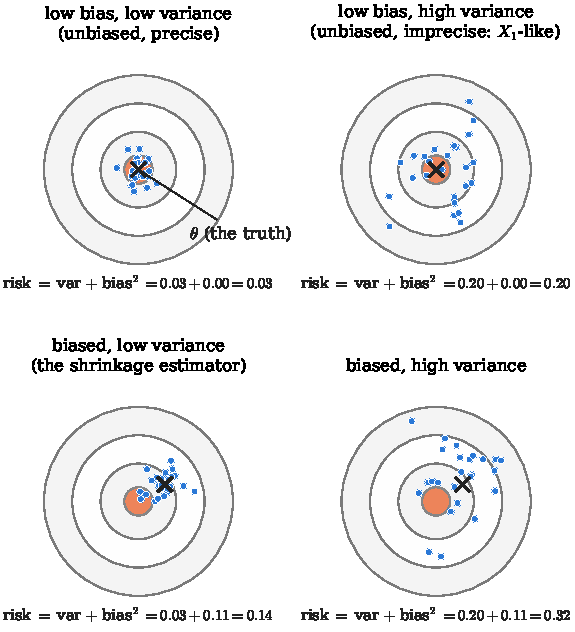
\includegraphics[width=0.78\textwidth]{fig_target}
\caption{Bias and variance as a target, in the four combinations. The bull's-eye is the truth $\theta$; each blue dot is the estimate from one sample; the black cross is the center of the group, $\E[\ethn]$.}
\label{fig:target}
\end{figure}

The target picture also settles a question the earlier bridge on $n - 1$ left open: Unbiased is not the same as closest.

\begin{bridge}[the $n - 1$ story, finished]
Among estimators of the form $c\sum_i (X_i - \bar{X}_n)^2$, the unbiased $S^2$ is not the one with the smallest quadratic risk.
For Gaussian data, dividing by $n + 1$ instead gives a biased estimator with strictly smaller quadratic risk than both the $n$ and $n - 1$ versions.
It is rarely used, since unbiasedness is a convention that makes results comparable across studies.
At $n = 12$ the risks are $0.182\sigma^4$, $0.160\sigma^4$ and $0.154\sigma^4$ for the divisors $n - 1$, $n$ and $n + 1$, and \cref{ex:t-nplus1} proves the general case.
\end{bridge}

\section{Strengths and weaknesses of estimators}
\label{sec:est-strengths}

Everything in this chapter can be applied at once to three estimators of $p$ for $\Xton \iid \Bern(p)$, $n$ large: $\bar{X}_n$, the constant $0.5$, and $X_1$.
Four criteria: bias, consistency, whether the estimator is efficiently computable (in this section, whether there is an explicit formula for it; the maximum likelihood estimators of \cref{ch:glm-links} have no closed form and are found by an iterative algorithm instead), and whether the quadratic risk tends to $0$ as $n \to \infty$.

\begin{center}
\small
\begin{tabular}{@{}l>{\raggedright\arraybackslash}p{1.1in}>{\raggedright\arraybackslash}p{1.1in}>{\raggedright\arraybackslash}p{1.1in}>{\raggedright\arraybackslash}p{1.3in}@{}}
\toprule
Estimator & Bias & Consistent? & Explicit formula? & Risk $\to 0$? \\
\midrule
$\bar{X}_n$ & $0$ & yes (LLN) & yes & yes: $p(1-p)/n$ \\[2pt]
$0.5$ & $0.5 - p$, nonzero unless $p = \frac12$ & no, unless $p = \frac12$ & yes & no: $(0.5 - p)^2$ for every $n$ \\[2pt]
$X_1$ & $0$ & no: it's $0$ or $1$, never near $p$ & yes & no: $p(1-p)$ for every $n$ \\
\bottomrule
\end{tabular}
\end{center}

The constant $0.5$ uses none of the data, so nothing can be learned from it; its only virtue is that it's exactly right when $p = \frac12$.
$X_1$ is unbiased, which sounds good, and uses one observation out of $n$, which is the actual problem: its risk doesn't shrink, so its accuracy is limited no matter how many samples are collected.
$\bar{X}_n$ has every property on the list.
Unbiasedness is desirable and may be the first thing to check, but the comparison with $X_1$ shows why it isn't enough: there are estimators that are unbiased and have a lot of variability, and risk is the number that catches them.

\begin{bridge}[random sampling for bias, a larger sample for variability]
An introductory course often draws the four targets of \cref{fig:target} with two rules: random sampling reduces bias, and a larger sample reduces variability.
The two rules act on the two terms of \cref{thm:bias-variance}.
Random sampling makes each $R_i$ a draw from $\Bern(p)$ with $p$ the population's proportion, which is all that $\E[\bar{R}_n] = p$ needs.
A design that over-represents part of the population draws from $\Bern(p')$ instead, with $p' \neq p$, so $\bar{R}_n$ is unbiased and consistent for $p'$, and as an estimator of $p$ it has
\[
R(\bar{R}_n) = \frac{p'(1 - p')}{n} + (p' - p)^2,
\]
of which a larger sample shrinks only the first term.
The 1936 \textit{Literary Digest} poll had about $2.4$ million returned ballots and predicted that Landon would beat Roosevelt $57\%$ to $43\%$; of the votes cast for the two, Roosevelt won $62\%$ (Freedman, Pisani and Purves, \textit{Statistics}).
With $p' = 0.43$ and $p = 0.62$ the first term is $1.0 \times 10^{-7}$, a standard deviation of $0.0003$, and the second is $0.036$: the risk was almost all bias, a miss of $19$ points.
\end{bridge}

\section{What comes next}
\label{sec:est-next}

Asymptotic normality hands you a sentence, `the error of $\ethn$ is approximately $\Gauss(0, \sigma^2/n)$', and the next two chapters are the two ways of using it.
\Cref{ch:confidence-intervals} turns it into a range of plausible values of $\theta$ with a guaranteed capture rate; \cref{ch:tests-foundations} turns it into a yes/no decision about $\theta$ with a guaranteed error rate.
Both need the quantiles of \cref{ch:gaussian} and the plug-in step of \cref{ch:limit-tools}, since $\sigma^2$ usually depends on $\theta$.

\section{Summary}
\label{sec:est-summary}

\begin{itemize}[nosep]
\item A statistic is a function of the data; an estimator of $\theta$ is a statistic whose formula doesn't involve $\theta$. Both are random variables. A statistic partitions the sample space and keeps one number per cell; a sufficient statistic keeps everything the sample says about $\theta$.
\item Consistent: $\ethn \convp \theta$ under $\Pr_\theta$, for every $\theta$. The sample mean is $\sqrt{n}$-consistent: its error is of exact order $1/\sqrt{n}$ (\cref{ex:rate}). Asymptotically normal: $\sqrt{n}(\ethn - \theta) \convd \Gauss(0, \sigma^2)$; $\sigma^2$ is the asymptotic variance, the variance of the limiting Gaussian, which for the sample mean equals $n \var(\bar{X}_n)$ and is never the limit of $\var(\ethn)$, which for any estimator whose variance shrinks is $0$ and carries no information.
\item Bias: $\E[\ethn] - \theta$. Unbiased means right on average. Convex or concave functions of unbiased estimators are biased, in the direction Jensen's inequality says: $g(\E[X]) \leq \E[g(X)]$ for convex $g$.
\item Variance: spread of $\ethn$ around its own mean. Using more of the data lowers it.
\item Quadratic risk: $\E[(\ethn - \theta)^2] = \var + \Bias^2$. It depends on $\theta$; a biased estimator can have lower risk than an unbiased one, and no estimator has the lowest risk for every $\theta$.
\item Of $\bar{X}_n$, the constant $\frac12$ and $X_1$, only $\bar{X}_n$ is unbiased, consistent and has risk tending to $0$. Unbiasedness alone, as $X_1$ shows, is not enough.
\end{itemize}

\section{Exercises}
\label{sec:est-exercises}

\begin{exercise}
Let $\Xton \iid \text{Unif}([a, a+1])$. Find $\E[\bar{X}_n]$, the bias of $\bar{X}_n$ for $a$, $\var(\bar{X}_n)$, and the quadratic risk of $\bar{X}_n - \frac12$.
\end{exercise}
\begin{solution}
$\E[\bar{X}_n] = a + \frac12$, bias $\frac12$. $\var(X_1) = \int_a^{a+1} x^2 \, \mathrm{d}x - (a + \frac12)^2 = a^2 + a + \frac13 - a^2 - a - \frac14 = \frac{1}{12}$, so $\var(\bar{X}_n) = \frac{1}{12n}$. The estimator $\bar{X}_n - \frac12$ is unbiased with the same variance, so its risk is $\frac{1}{12n}$, which tends to $0$.
\end{solution}

\begin{exercise}
Let $\Xton \iid \Bern(p)$ and $\hat{p} = \sqrt{\ind(X_1 = 1, X_2 = 1)}$. Find its bias, variance and quadratic risk, and say whether it is consistent.
\end{exercise}
\begin{solution}
$\hat{p} \sim \Bern(p^2)$, so bias $= p^2 - p$, variance $= p^2(1-p^2)$, and risk $= p^2(1-p^2) + (p^2 - p)^2 = p^2(1 - p^2) + p^2(1-p)^2$. None of these depend on $n$, so the risk does not go to $0$. The estimator is not consistent either, for the direct reason that its distribution never changes with $n$: $\Pr(\abs{\hat{p} - p} > \epsilon)$ is the same positive number for every $n$. It never uses $X_3, \ldots, X_n$.
\end{solution}

\begin{exercise}
In the kiss model with $n = 124$, compute the bias, variance and risk of the shrinkage estimator $\tilde{p}_n = (n \bar{R}_n + 10)/(n + 20)$ at $p = 0.645$ and at $p = 0.9$, and compare each with $\bar{R}_n$.
\end{exercise}
\begin{solution}
$\E[\tilde{p}_n] = (np + 10)/(n + 20)$ and $\var(\tilde{p}_n) = n p(1-p)/(n+20)^2$. At $p = 0.645$: mean $0.6249$, bias $-0.0201$, variance $0.001369$, risk $0.001775$, against $\bar{R}_n$'s risk $0.001847$. At $p = 0.9$: mean $0.8444$, bias $-0.0556$, variance $0.000538$, risk $0.003625$, against $\bar{R}_n$'s $0.000726$. Shrinking toward $\frac12$ pays when $p$ is near $\frac12$ and costs five times over when it isn't; \cref{fig:biasvariance} shows the crossover at $p \approx 0.34$ and $0.66$.
\end{solution}

\begin{exercise}
Let $\Xton \iid \Expo(\lambda)$ and $\hat{\lambda} = 1/\bar{X}_n$. Use Jensen's inequality to determine the sign of the bias, and use the fact (which you may take as given) that $\bar{X}_n$ has the Gamma distribution with $\E[1/\bar{X}_n] = \frac{n}{n-1} \lambda$ for $n \geq 2$ to find the bias exactly. Is there an unbiased estimator of $\lambda$ of the form $c/\bar{X}_n$?
\end{exercise}
\begin{solution}
$g(x) = 1/x$ is convex on $(0,\infty)$, so $\E[1/\bar{X}_n] \geq 1/\E[\bar{X}_n] = \lambda$: the bias is non-negative. Exactly, the bias is $\frac{n}{n-1}\lambda - \lambda = \frac{\lambda}{n-1}$, positive and of order $1/n$. The estimator $\frac{n-1}{n} \cdot \frac{1}{\bar{X}_n} = (n-1)/\sum X_i$ is unbiased.
\end{solution}

\begin{exercise}
Show that an estimator whose bias and variance both tend to $0$ is consistent. Is the converse true?
\end{exercise}
\begin{solution}
Bias and variance tending to $0$ means $R(\ethn) = \E[(\ethn - \theta)^2] \to 0$, which implies convergence in probability by Chebyshev's inequality (\cref{prop:shrinking-variance}; in the language of \cref{app:modes}, convergence in quadratic mean implies convergence in probability). The converse fails: convergence in probability does not require any moments to exist. For an example, take $\ethn = \theta$ with probability $1 - 1/n$ and $\ethn = n$ with probability $1/n$; then $\ethn \convp \theta$, but $\E[\ethn] = \theta(1 - 1/n) + 1 \to \theta + 1$, so the bias tends to $1$, not $0$.
\end{solution}

\chapter{Confidence Intervals}
\label{ch:confidence-intervals}

\begin{chaptergoals}
\begin{itemize}[nosep]
\item What a confidence interval is: a \textit{random} interval, computable from the data alone, that traps the fixed parameter with a guaranteed probability. The two words that carry the definition are `random' and `computable'.
\item The recipe that produces every interval in this book: find a pivot (a quantity whose distribution you know), trap it between two quantiles, solve for the parameter. An exact pivot gives an exact interval; the CLT gives an asymptotic one.
\item Three ways around a pivot whose scale involves the unknown parameter: conservative, solve, plug-in. One picture explains all three and shows how they nest.
\item What drives the width (the level, through a quantile; the sample size, through $1/\sqrt{n}$), and what the $95\%$ does and does not mean.
\end{itemize}
The running examples are the kiss experiment ($n = 124$, $\bar{R}_n = 0.645$), for which \cref{ch:kiss} promised the interval $[0.56, 0.73]$, and the subway inter-arrival times of \cref{ch:limit-tools} ($n = 64$, $\bar{T}_n = 6.23$).
\end{chaptergoals}

\section{What a confidence interval is}
\label{sec:ci-definition}

\Cref{ch:estimators} produced a number, $\hat{p} = 0.645$, and a sampling distribution around it.
A confidence interval converts the two into a statement with a guarantee: a range of values of $p$, and a probability that the range is right.

\begin{definition}[Confidence interval]
\label{def:ci}
Let $\statmodel$ be a statistical model based on observations $\Xton$, with $\Theta \subseteq \real$, and let $\alpha \in (0,1)$.

A \textbf{confidence interval of level $1 - \alpha$} for $\theta$ is a random interval $\mathcal{I} = [L(\Xton), \, U(\Xton)]$ whose endpoints are statistics (their formulas don't involve $\theta$), such that
\[
\Pr_\theta \left( \mathcal{I} \ni \theta \right) \geq 1 - \alpha \quad \text{for all } \theta \in \Theta.
\]

A confidence interval of \textbf{asymptotic level $1 - \alpha$} is a random interval $\mathcal{I} = \mathcal{I}_n$ of the same kind such that
\[
\limn \Pr_\theta \left( \mathcal{I}_n \ni \theta \right) \geq 1 - \alpha \quad \text{for all } \theta \in \Theta.
\]
\end{definition}

\begin{inwords}
\textbf{In words.} A rule that turns a sample into an interval, computable from the sample alone, such that the interval it produces contains the true parameter at least $100(1 - \alpha)\%$ of the time, whatever the true parameter is. `Asymptotic' means the guarantee holds in the limit of large samples.
\par\smallskip
\textbf{For the kiss data.} The rule `$\bar{R}_n \pm 1.96\sqrt{\bar{R}_n(1 - \bar{R}_n)/n}$' is a confidence interval of asymptotic level $95\%$; on this sample it produced $[0.56, 0.73]$. The rule `$\bar{R}_n \pm 1.96\sqrt{p(1-p)/n}$' is not one, since $p$ is in its formula.
\end{inwords}

The notation $\mathcal{I} \ni \theta$ says `$\mathcal{I}$ contains $\theta$'.
It means the same as $\theta \in \mathcal{I}$, and this book writes it backwards on purpose: the random object, the thing the probability is about, is the interval on the left, not the parameter on the right.
Both appearances of $\theta$ in $\Pr_\theta(\mathcal{I} \ni \theta)$ are the same fixed number doing two jobs: as the subscript it fixes which distribution the sample is drawn from, and inside the parentheses it is the target that the interval either contains or misses.
Nothing in the expression is random except $\mathcal{I}$.

Three things in the definition deserve a second look.

\begin{enumerate}[nosep]
\item \textit{The interval is random; the parameter is not.} $L$ and $U$ are functions of the sample, so they're random variables, and $\mathcal{I}$ moves from sample to sample. $\theta$ is a fixed number that doesn't move. The probability is the probability that the moving interval lands on the fixed point.
\item \textit{The endpoints must be computable.} An interval whose formula contains $\theta$ is not a confidence interval, however nice its coverage probability: you can't compute it. This clause is what the three `solutions' of \cref{sec:ci-three-solutions} are solutions to.
\item \textit{The guarantee holds for every $\theta$.} You don't know $\theta$, so a guarantee that holds for some values of it and not others is no guarantee. This clause is what makes one of the intervals in \cref{ex:ci-fifty} fail.
\end{enumerate}

The inequality $\geq 1 - \alpha$ has a consequence worth stating once: a confidence interval of level $95\%$ is also a confidence interval of level $90\%$, of level $50\%$, of any level below $95\%$.
It is not, in general, one of level $98\%$.
`Level' is a floor on the coverage, not its exact value.

The word `level' is used for tests too (\cref{ch:tests-foundations}), where it denotes $\alpha$, the probability of rejecting a true hypothesis; for an interval the level is $1 - \alpha$, the probability of a correct capture.
Same $\alpha$, complementary conventions, and the context always says which is meant.

\begin{intuition}[a procedure, not a number]
The confidence interval is the \textit{rule} that turns a sample into an interval, $(x_1, \ldots, x_n) \mapsto [L, U]$, and the level is a property of the rule: the fraction of samples on which the rule's output contains $\theta$.
Once you apply the rule to your one sample you get two numbers, $[0.56, 0.73]$.
Those numbers are not random and the parameter is not random, so the pair has no probability attached: $[0.56, 0.73]$ either contains $p$ or it doesn't, and you will never know which.
What you know is that the rule that produced it is right $95\%$ of the time.
\Cref{fig:cirepeated} is this sentence as a picture.
The kiss experiment was simulated $100$ times with $n = 124$ and $p = 0.645$, and the plug-in interval of \cref{sec:ci-three-solutions} was computed each time.
The parameter is the fixed vertical line; the intervals move, and each is centered at its own $\hat{p}$.
Sorted by $\hat{p}$, the six that miss are the samples whose proportion came out unusually low or high.
Ninety-four of the hundred contain $0.645$ and six don't, and the level $95\%$ is the long-run rate of the first kind, not a statement about any one of the hundred intervals.
\end{intuition}

\begin{figure}[htbp]
\centering
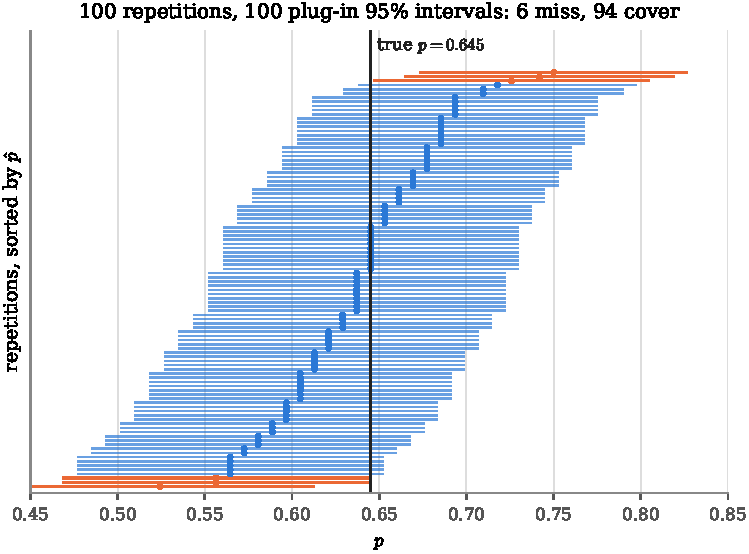
\includegraphics[width=\textwidth]{fig_ci_repeated}
\caption{One hundred simulated kiss experiments with $n = 124$ and $p = 0.645$, sorted by $\hat{p}$ (dot), each with its $95\%$ plug-in interval. The black vertical line is $p$; intervals that contain it are blue, the six that miss are orange.}
\label{fig:cirepeated}
\end{figure}

\section{The recipe, on an exact case}
\label{sec:ci-recipe}

Every interval in this book is built the same way, and the cleanest place to see the construction is the one case where nothing is asymptotic.

\begin{worked}[Gaussian data, known variance]
Let $\Xton \iid \Gauss(\mu, \sigma^2)$ with $\sigma^2$ known and $\mu$ unknown.
By \cref{ch:gaussian}, $\bar{X}_n \sim \Gauss(\mu, \sigma^2/n)$ exactly, for every $n$, so
\[
Z = \sqrt{n} \, \frac{\bar{X}_n - \mu}{\sigma} \sim \Gauss(0, 1) \quad \text{for every } n \text{ and every } \mu.
\]
A quantity like $Z$, a function of the data and the parameter whose distribution doesn't depend on the parameter, is called a \textbf{pivot}.
The recipe has three steps.
\begin{enumerate}[nosep]
\item \textit{Trap the pivot.} With $q_{\alpha/2}$ the quantile of \cref{sec:gauss-quantiles}, $\Pr(-q_{\alpha/2} \leq Z \leq q_{\alpha/2}) = 1 - \alpha$.
\item \textit{Rewrite the event.} $-q_{\alpha/2} \leq \sqrt{n}(\bar{X}_n - \mu)/\sigma \leq q_{\alpha/2}$ is the same event as $\abs{\bar{X}_n - \mu} \leq q_{\alpha/2} \, \sigma/\sqrt{n}$.
\item \textit{Solve for the parameter.} That event is the same as
\[
\mu \in \left[ \bar{X}_n - q_{\alpha/2} \frac{\sigma}{\sqrt{n}}, \; \bar{X}_n + q_{\alpha/2} \frac{\sigma}{\sqrt{n}} \right] =: \mathcal{I}.
\]
\end{enumerate}
The event in step 3 is the event in step 1, written differently, so $\Pr_\mu(\mathcal{I} \ni \mu) = 1 - \alpha$ for every $\mu$ and every $n$.
The endpoints involve $\bar{X}_n$, $\sigma$ (known), $n$ and a quantile, none of which is $\mu$, so $\mathcal{I}$ is a confidence interval of level $1 - \alpha$, with no limit anywhere.
For $\alpha = 0.05$ it is $\bar{X}_n \pm 1.96 \, \sigma/\sqrt{n}$.
\end{worked}

\begin{bridge}[estimate $\pm$ margin of error]
The interval you learned is `point estimate $\pm$ (critical value) $\times$ (standard error)'.
The recipe says where each piece comes from: the point estimate is the center because the pivot is centered at the parameter; the critical value is the quantile that traps the pivot; the standard error is the pivot's scale, $\sigma/\sqrt{n}$.
When $\sigma$ is unknown, an introductory course replaces it by $s$ and switches to a $t$ critical value: that is a different pivot, $\sqrt{n}(\bar{X}_n - \mu)/s$, with an exact Student distribution for Gaussian data, and \cref{ch:t-test} derives it.
For large $n$ and any parent distribution, the replacement is justified by Slutsky instead (\cref{sec:slutsky}), which is the route this chapter takes.
\end{bridge}

\textbf{One-sided intervals.}
Nothing forces step 1 to trap the pivot symmetrically.
$\Pr(Z \leq q_\alpha) = 1 - \alpha$ as well, and solving $\sqrt{n}(\bar{X}_n - \mu)/\sigma \leq q_\alpha$ for $\mu$ gives
\[
\mu \in \left[ \bar{X}_n - q_\alpha \frac{\sigma}{\sqrt{n}}, \; \infty \right),
\]
a \textbf{lower confidence bound}: `$\mu$ is at least this much', with level $1 - \alpha$.
Trapping $Z \geq -q_\alpha$ gives the upper bound $(-\infty, \bar{X}_n + q_\alpha \sigma/\sqrt{n}]$.
Note the quantile: $q_\alpha$ ($1.645$ at $95\%$), not $q_{\alpha/2}$ ($1.96$) because all of the $5\%$ of misses is spent on one side.
One-sided intervals are the confidence-interval face of one-sided tests, and \cref{ex:ci-onesided} makes the correspondence exact.

\section{The kiss experiment: an interval that isn't one}
\label{sec:ci-kiss-problem}

Now $R_1, \ldots, R_n \iid \Bern(p)$, $\hat{p} = \bar{R}_n$, and there is no exact pivot in sight: the distribution of $\bar{R}_n$ is Binomial, scaled, and it depends on $p$ in a way that no simple transformation removes.
What there is instead is the CLT (\cref{thm:clt}).
\recall{The Central Limit Theorem says that the error of an average, magnified by $\sqrt{n}$ and divided by the standard deviation of one observation, has a distribution that settles down to $\Gauss(0,1)$, whatever the observations were drawn from. You do not need to know that distribution to use the theorem; you need only its mean and variance.}
\[
\sqrt{n} \, \frac{\bar{R}_n - p}{\sqrt{p(1-p)}} \convd \Gauss(0, 1).
\]
The left side is an \textit{asymptotic} pivot: its distribution depends on $p$ for every finite $n$, but its limit doesn't.
Convergence in distribution means convergence of the CDF at every continuity point of the limit (\cref{sec:conv-dist}), and the Gaussian CDF is continuous everywhere, so
\[
\limn \Pr_p \left( -q_{\alpha/2} \leq \sqrt{n} \, \frac{\bar{R}_n - p}{\sqrt{p(1-p)}} \leq q_{\alpha/2} \right) = \Pr(-q_{\alpha/2} \leq Z \leq q_{\alpha/2}) = 1 - \alpha.
\]
Steps 2 and 3 of the recipe then give
\begin{equation}
\label{eq:ci-not-a-ci}
\limn \Pr_p \left( \left[ \bar{R}_n - q_{\alpha/2} \sqrt{\frac{p(1-p)}{n}}, \; \bar{R}_n + q_{\alpha/2} \sqrt{\frac{p(1-p)}{n}} \right] \ni p \right) = 1 - \alpha.
\end{equation}
This looks like the Gaussian case with $\sigma$ replaced by $\sqrt{p(1-p)}$, and it has the right asymptotic coverage, \textit{but it is not a confidence interval}: the endpoints contain $p$.
You can't compute $\bar{R}_n \pm 1.96 \sqrt{p(1-p)/124}$ without knowing the thing you're estimating.
The pivot's scale depends on the parameter, and the recipe's step 3 is stuck.

\begin{figure}[htbp]
\centering
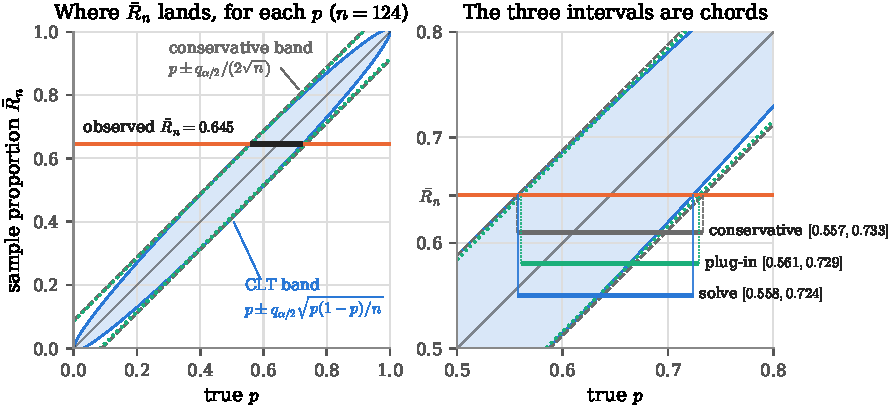
\includegraphics[width=\textwidth]{fig_ci_inversion}
\caption{Sample proportion against the true $p$, $n = 124$. Left: the CLT band $p \pm q_{\alpha/2}\sqrt{p(1-p)/n}$ (blue), the widest band (gray dashes), a band of constant width (aqua dots) and the observed $\bar{R}_n = 0.645$ (orange line). Right: the three chords, to scale.}
\label{fig:ciinversion}
\end{figure}

\section{Three ways to get unstuck}
\label{sec:ci-three-solutions}

\Cref{fig:ciinversion} is the picture to hold on to.
For each candidate value of $p$ on the horizontal axis, the CLT band is the set of sample proportions that value would plausibly produce: by \cref{eq:ci-not-a-ci}, $\bar{R}_n$ lands in $p \pm q_{\alpha/2}\sqrt{p(1-p)/n}$ about $95\%$ of the time, and the band is a lens, widest at $p = \frac12$ and pinched at the ends.
Reading the picture downwards, from a $p$ to its band, is probability.
Reading it sideways, from the observed $\bar{R}_n = 0.645$ (the horizontal line) to the set of $p$ whose bands reach it, is statistics, and that set is the confidence interval.
With the lens itself, it is the chord the line cuts out of the lens, and that chord is the solve interval.
The three solutions differ in which band they read.
The conservative interval replaces the lens by the widest band it fits in, and gets a longer chord.
The plug-in interval replaces the lens by a band of constant width $q_{\alpha/2}\sqrt{\hat{p}(1-\hat{p})/n}$, the width the lens has at $p = \hat{p}$, and gets a chord of nearly the same length, centered at $\hat{p}$.
The right of the figure shows the three chords to scale, with $n = 124$.

\subsection*{Solution 1: conservative}

Whatever $p$ is, $p(1-p) \leq \frac14$, with equality at $p = \frac12$.
So the event in \cref{eq:ci-not-a-ci} is contained in a larger event with a computable boundary:
\[
\abs{\bar{R}_n - p} \leq q_{\alpha/2} \sqrt{\frac{p(1-p)}{n}} \quad \Longrightarrow \quad \abs{\bar{R}_n - p} \leq \frac{q_{\alpha/2}}{2\sqrt{n}}.
\]
Define
\[
\mathcal{I}_{\text{conserv}} = \left[ \bar{R}_n - \frac{q_{\alpha/2}}{2\sqrt{n}}, \; \bar{R}_n + \frac{q_{\alpha/2}}{2\sqrt{n}} \right].
\]
Its coverage is at least that of the CLT event, so $\limn \Pr_p(\mathcal{I}_{\text{conserv}} \ni p) \geq 1 - \alpha$ for every $p$: an asymptotic confidence interval, with the inequality of the definition used in earnest.
The coverage is exactly $1 - \alpha$ in the limit only at $p = \frac12$; elsewhere the interval is wider than it needs to be, which is what `conservative' means.
In the figure it reads the widest band instead of the lens.

With $n = 124$: $q_{0.025}/(2\sqrt{124}) = 1.96/22.27 = 0.088$, so $\mathcal{I}_{\text{conserv}} = [0.557, 0.733]$.

\subsection*{Solution 2: solve}

Keep the lens and do step 3 properly.
The event $\abs{\bar{R}_n - p} \leq q_{\alpha/2}\sqrt{p(1-p)/n}$ is, after squaring,
\[
(\bar{R}_n - p)^2 \leq \frac{q_{\alpha/2}^2}{n} \, p(1-p),
\qquad \text{that is,} \qquad
\left( 1 + \frac{q_{\alpha/2}^2}{n} \right) p^2 - \left( 2\bar{R}_n + \frac{q_{\alpha/2}^2}{n} \right) p + \bar{R}_n^2 \leq 0.
\]
The left side is a convex quadratic in $p$, so the inequality holds exactly between its two roots $p_1 < p_2$, and
\[
\mathcal{I}_{\text{solve}} = [p_1, p_2]
\]
is the \textit{same event} as the one in \cref{eq:ci-not-a-ci}, now with computable endpoints: $\limn \Pr_p(\mathcal{I}_{\text{solve}} \ni p) = 1 - \alpha$, with equality.
The quadratic formula gives the roots in closed form,
\begin{equation}
\label{eq:wilson}
p_{1,2} = \frac{1}{1 + q_{\alpha/2}^2/n} \left( \bar{R}_n + \frac{q_{\alpha/2}^2}{2n} \; \mp \; q_{\alpha/2} \sqrt{ \frac{\bar{R}_n(1 - \bar{R}_n)}{n} + \frac{q_{\alpha/2}^2}{4n^2} } \right),
\end{equation}
an interval known as the Wilson score interval.
The word `score' is explained in \cref{sec:tests-duality}: this interval is what you get by inverting a standard test of $H_0: p = p_0$, the score test, which measures distance from $p_0$ in units of the standard error computed at $p_0$.
Note that it is \textit{not} centered at $\bar{R}_n$: its center is pulled toward $\frac12$, by an amount of order $1/n$ because the lens is wider there.

With $n = 124$, $\bar{R}_n = 80/124$ and $q_{0.025} = 1.96$ the quadratic is $1.0310\,p^2 - 1.3213\,p + 0.4162 \leq 0$, with roots $p_1 = 0.558$ and $p_2 = 0.724$: $\mathcal{I}_{\text{solve}} = [0.558, 0.724]$.

\begin{pitfall}[rounding the quadratic before solving it]
Solve for $p_1$ and $p_2$ from the coefficients as computed, not from rounded versions of them.
A quadratic's roots are sensitive to its coefficients, and this quadratic is a bad case.
Its constant term is $0.4162$; carrying that to two decimals as $0.41$ moves the roots three points each way, to $[0.53, 0.75]$, and rounding it up to $0.42$ instead gives $[0.59, 0.69]$, wrong in the other direction.
Two decimals are not enough here either way, and the error is large enough to change the conclusion: the $[0.53, 0.75]$ that the truncated coefficients produce is wider than the conservative interval $[0.557, 0.733]$, while the true solve interval $[0.558, 0.724]$ is the narrowest of the three.
The solve interval can never be the widest, since \cref{prop:ci-nesting} shows it always sits inside the conservative interval, so an interval that comes out wider than the conservative one is an arithmetic error and nothing else.
\end{pitfall}

\subsection*{Solution 3: plug-in}

Replace the unknown scale $\sqrt{p(1-p)}$ by its estimate $\sqrt{\hat{p}(1 - \hat{p})}$, and let Slutsky's theorem pay for it.
\recall{Slutsky's theorem is the rule that lets you substitute an estimate for an unknown constant inside a limit: if one quantity settles into a distribution and a second converges in probability to a constant, their product and their sum behave as if the second simply \textit{were} that constant. It is what makes every `estimate $\pm$ standard error' formula legitimate.}
This is the worked example of \cref{sec:slutsky}: since $\hat{p} \convp p$ (LLN) and $x \mapsto \sqrt{p(1-p)/(x(1-x))}$ is continuous at $p$ (CMT),
\[
\sqrt{n} \, \frac{\bar{R}_n - p}{\sqrt{\hat{p}(1 - \hat{p})}}
= \underbrace{\sqrt{n} \, \frac{\bar{R}_n - p}{\sqrt{p(1-p)}}}_{\convd \Gauss(0,1)} \cdot \underbrace{\sqrt{\frac{p(1-p)}{\hat{p}(1-\hat{p})}}}_{\convp 1} \convd \Gauss(0,1).
\]
The left side is a new asymptotic pivot whose scale no longer involves $p$, so the recipe runs to the end:
\[
\mathcal{I}_{\text{plug-in}} = \left[ \bar{R}_n - q_{\alpha/2} \sqrt{\frac{\hat{p}(1-\hat{p})}{n}}, \; \bar{R}_n + q_{\alpha/2} \sqrt{\frac{\hat{p}(1-\hat{p})}{n}} \right],
\qquad \limn \Pr_p(\mathcal{I}_{\text{plug-in}} \ni p) = 1 - \alpha.
\]
In the figure it reads a band of constant width, the lens's width at $\hat{p}$.
The price is a second asymptotic approximation on top of the CLT: Slutsky's theorem is a statement about $n \to \infty$, and at finite $n$ the estimated scale is itself noisy.

With $n = 124$: $1.96 \sqrt{0.645 \times 0.355/124} = 0.084$, so $\mathcal{I}_{\text{plug-in}} = [0.561, 0.729]$.

\subsection*{The three side by side}

\begin{center}
\begin{tabular}{@{}ll>{\raggedright\arraybackslash}p{3.6cm}>{\raggedright\arraybackslash}p{4.6cm}@{}}
\toprule
Interval & $95\%$, $n = 124$ & Reads & Asymptotic coverage \\
\midrule
conservative & $[0.557, 0.733]$ & the widest band & $\geq 1 - \alpha$; $= 1 - \alpha$ only at $p = \frac12$ \\[2pt]
solve & $[0.558, 0.724]$ & the lens itself & $= 1 - \alpha$; one approximation (CLT) \\[2pt]
plug-in & $[0.561, 0.729]$ & a band of half-width $q_{\alpha/2}\sqrt{\hat{p}(1-\hat{p})/n}$ & $= 1 - \alpha$; two approximations (CLT, Slutsky) \\
\bottomrule
\end{tabular}
\end{center}

The conservative and plug-in intervals round to the $[0.56, 0.73]$ that \cref{ch:kiss} promised, the solve interval to $[0.56, 0.72]$, and \cref{ch:kiss}'s drug example is the same computation: $78$ of $100$ cured gives $\hat{p} = 0.78$ and $\mathcal{I}_{\text{plug-in}} = 0.78 \pm 1.96\sqrt{0.78 \times 0.22/100} = [0.699, 0.861]$, the $[0.70, 0.86]$ quoted there.
There are more intervals still; the exact interval built from the Binomial distribution of $n\bar{R}_n$ rather than from the CLT (the Clopper--Pearson interval mentioned in \cref{sec:conv-what-limits-buy}) gives $[0.554, 0.729]$ for the kiss data, and Newcombe (1998) compares seven of them on coverage and width.\footnote{R.\ Newcombe, `Two-sided confidence intervals for the single proportion: comparison of seven methods', \textit{Statistics in Medicine} 17 (1998).}
That they all agree to within a point is the CLT doing its job at $n = 124$.

\begin{proposition}[How the three nest]
\label{prop:ci-nesting}
For every sample and every $n$: $\mathcal{I}_{\text{solve}} \subseteq \mathcal{I}_{\text{conserv}}$ and $\mathcal{I}_{\text{plug-in}} \subseteq \mathcal{I}_{\text{conserv}}$, and both $\mathcal{I}_{\text{solve}}$ and $\mathcal{I}_{\text{plug-in}}$ contain $\bar{R}_n$.
\end{proposition}
\coreproof{Everything follows from $p(1-p) \leq \frac14$: a $p$ that passes the solve test passes the conservative one, and the plug-in half-width is at most the conservative half-width.}
\begin{proof}
If $p \in \mathcal{I}_{\text{solve}}$ then $\abs{\bar{R}_n - p} \leq q_{\alpha/2}\sqrt{p(1-p)/n} \leq q_{\alpha/2}/(2\sqrt{n})$, so $p \in \mathcal{I}_{\text{conserv}}$.
The plug-in half-width is $q_{\alpha/2}\sqrt{\hat{p}(1-\hat{p})/n} \leq q_{\alpha/2}/(2\sqrt{n})$, the conservative one.
Finally $p = \bar{R}_n$ satisfies the solve inequality trivially ($0 \leq$ something non-negative), and the plug-in interval is centered there.
\end{proof}

In the picture: the lens lies inside the widest band, so any chord of the lens lies inside the corresponding chord of the band.
Solve and plug-in need not nest with each other; here the solve interval is shifted toward $\frac12$ and slightly shorter.

\begin{intuition}[which one to use]
Use the solve interval for a proportion, the plug-in interval for everything else.
The defense: the solve interval has the exact asymptotic level with one approximation, has a closed form (\cref{eq:wilson}) and, as \cref{fig:cicoverage} shows, holds up at finite $n$ far better than the plug-in interval near $p = 0$ or $1$, where the latter breaks; the only reason it isn't universal is that `solve for the parameter' is a quadratic here and may be intractable elsewhere.
The plug-in interval is the one every formula sheet gives, is what the next chapters use, and is fine whenever $n\hat{p}(1-\hat{p})$ is comfortably large; \cref{ch:wald-lrt} identifies it as an inverted Wald test and, for models other than the proportion, recommends the likelihood ratio interval in its place.
The conservative interval is for two jobs: a guaranteed level, and planning sample sizes before any data exist (\cref{sec:ci-width}), since it is the only one of the three whose width you know in advance.
\end{intuition}

\section{What `asymptotic level' buys at a finite \texorpdfstring{$n$}{n}}
\label{sec:ci-coverage}

Asymptotic level $1 - \alpha$ is a promise about $n \to \infty$.
For a proportion you can check what it delivers at the $n$ you have because the distribution of $n\bar{R}_n$ is Binomial and the coverage probability is a finite sum:
\[
\Pr_p(\mathcal{I} \ni p) = \sum_{k=0}^{n} \binom{n}{k} p^k (1-p)^{n-k} \, \ind\big( \mathcal{I}(k) \ni p \big),
\]
where $\mathcal{I}(k)$ is the interval the rule produces when $k$ of the $n$ couples turn right.
\Cref{fig:cicoverage} plots this against $p$ for the three intervals, at $n = 124$ and at $n = 20$.
The conservative interval over-covers away from $p = \frac12$: its coverage is $0.99995$ at $p = 0.05$.
The plug-in interval under-covers, mildly at $n = 124$ ($0.939$ at $p = 0.645$) and badly at $n = 20$ near the edges.
The solve interval stays near $0.95$ at $n = 124$ ($0.952$ at $p = 0.645$) and above $0.92$ at $n = 20$ for $p$ between $0.01$ and $0.99$, where the plug-in interval falls as low as $0.33$, below the bottom of the plot.
The saw teeth are real, not noise: $\bar{R}_n$ takes only $n + 1$ values, so there are only $n + 1$ possible intervals, and the coverage jumps whenever $p$ crosses an endpoint of one of them.

\begin{figure}[htbp]
\centering
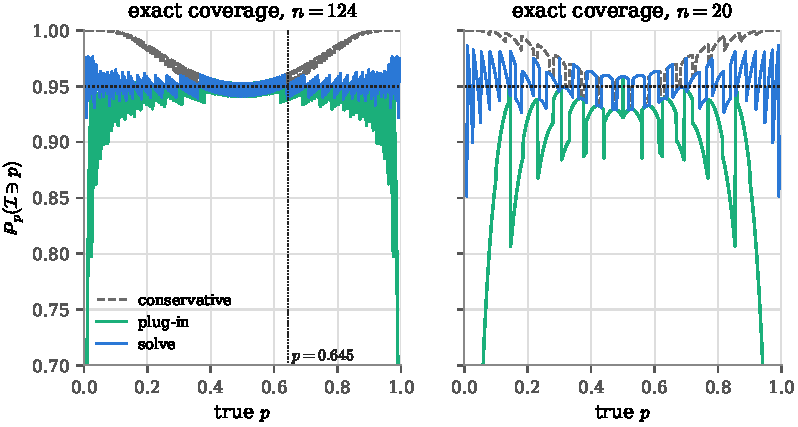
\includegraphics[width=\textwidth]{fig_ci_coverage}
\caption{Exact coverage probability $\Pr_p(\mathcal{I} \ni p)$ of the three $95\%$ intervals against the true $p$: conservative (gray dashes), plug-in (aqua) and solve (blue), with the nominal $0.95$ as a dotted line. Left, $n = 124$; right, $n = 20$.}
\label{fig:cicoverage}
\end{figure}

Three lessons from the figure.
The asymptotic promise is kept at $n = 124$ to within a point or two for $p$ in the middle of $(0,1)$, which is where the kiss data put it.
The plug-in interval is the one that fails first as $n$ shrinks or $p$ approaches the edges because its width is $\sqrt{\hat{p}(1-\hat{p})/n}$ and $\hat{p}$ near $0$ or $1$ makes it think it is very precise (at $\hat{p} = 0$ its width is zero).
And the conservative interval is not free: its extra width buys coverage you didn't ask for, and that over-coverage is wasted precision.

This is the chapter's instance of the book's stance on asymptotics (the intuition box that opens \cref{ch:lln}, and \cref{sec:conv-what-limits-buy}): the theorem licenses the Gaussian replacement and is silent about the error at your $n$.
For a proportion the error can be computed, as here.
For most models it can't, and the plug-in interval is used on trust and on the experience that $n$ in the dozens with a parameter away from the boundary is usually enough.

\section{The subway: when the scale depends on the parameter in a new way}
\label{sec:ci-subway}

The three solutions were introduced for a proportion, where the scale $\sqrt{p(1-p)}$ is bounded.
The inter-arrival-time example of \cref{sec:delta-method} shows what changes when it isn't.
$T_1, \ldots, T_n \iid \Expo(\lambda)$, $\hat{\lambda} = 1/\bar{T}_n$, and the delta method gave
\recall{The delta method says what happens to a transformed estimator: if $\hat\theta_n$ is approximately Gaussian around $\theta$ with standard deviation $\sigma/\sqrt{n}$, then $g(\hat\theta_n)$ is approximately Gaussian around $g(\theta)$ with standard deviation $\abs{g'(\theta)}\sigma/\sqrt{n}$. The slope of $g$ at $\theta$ stretches or compresses the error.}
\[
\sqrt{n} \, (\hat{\lambda} - \lambda) \convd \Gauss(0, \lambda^2),
\qquad \text{so} \qquad
\limn \Pr_\lambda \left( \abs{\hat{\lambda} - \lambda} \leq q_{\alpha/2} \frac{\lambda}{\sqrt{n}} \right) = 1 - \alpha.
\]
Again the half-width involves the parameter, now as a factor $\lambda$ rather than $\sqrt{p(1-p)}$, and \cref{fig:ciwedge} shows the consequence: the band is a wedge, not a lens.
For each true $\lambda$, the delta method says $\hat{\lambda}$ lands in $\lambda \pm q_{\alpha/2}\lambda/\sqrt{n}$ about $95\%$ of the time, and that band keeps opening as $\lambda$ grows, with no widest point.
The observed $\hat{\lambda} = 1/6.23 = 0.1605$ is the horizontal line, and the solve interval is the chord it cuts from the wedge, which is not centered at $\hat{\lambda}$ because the wedge is wider to the right.
The plug-in interval uses a band of constant width $q_{\alpha/2}\hat{\lambda}/\sqrt{n}$ and is centered.
No band of constant width contains the wedge, so there is nothing for a conservative interval to read.

\begin{figure}[htbp]
\centering
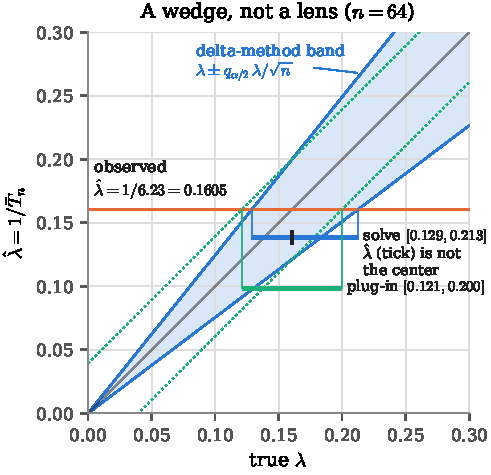
\includegraphics[width=0.62\textwidth]{fig_ci_wedge}
\caption{The subway rate, $n = 64$: $\hat{\lambda}$ against the true $\lambda$. The delta-method band $\lambda \pm q_{\alpha/2}\lambda/\sqrt{n}$ (blue), the plug-in band of constant width (aqua dots), the observed $\hat{\lambda} = 0.1605$ (orange line) and the two chords below it.}
\label{fig:ciwedge}
\end{figure}

\begin{enumerate}[nosep]
\item \textit{Conservative:} there is nothing to bound. $\lambda$ ranges over $(0, \infty)$, so $\sup_\lambda q_{\alpha/2}\lambda/\sqrt{n} = \infty$ and the `conservative interval' is $(0, \infty)$, which has level $100\%$ and says nothing.
\item \textit{Solve:} the inequality is linear in $\lambda$ this time. $\abs{\hat{\lambda} - \lambda} \leq q_{\alpha/2}\lambda/\sqrt{n}$ is the same as $\lambda(1 - q_{\alpha/2}/\sqrt{n}) \leq \hat{\lambda} \leq \lambda(1 + q_{\alpha/2}/\sqrt{n})$, and if $n > q_{\alpha/2}^2$ (so that $1 - q_{\alpha/2}/\sqrt{n} > 0$) this solves to
\[
\mathcal{I}_{\text{solve}} = \left[ \frac{\hat{\lambda}}{1 + q_{\alpha/2}/\sqrt{n}}, \; \frac{\hat{\lambda}}{1 - q_{\alpha/2}/\sqrt{n}} \right].
\]
\item \textit{Plug-in:} replace $\lambda$ in the half-width by $\hat{\lambda}$ (Slutsky, since $\hat{\lambda} \convp \lambda$):
\[
\mathcal{I}_{\text{plug-in}} = \left[ \hat{\lambda} \left( 1 - \frac{q_{\alpha/2}}{\sqrt{n}} \right), \; \hat{\lambda} \left( 1 + \frac{q_{\alpha/2}}{\sqrt{n}} \right) \right].
\]
\end{enumerate}
With $n = 64$ and $\bar{T}_n = 6.23$ minutes: $\hat{\lambda} = 0.1605$ per minute and $q_{0.025}/\sqrt{64} = 0.245$, so
\[
\mathcal{I}_{\text{solve}} = [0.129, 0.213] \approx [0.13, 0.21], \qquad \mathcal{I}_{\text{plug-in}} = [0.121, 0.200] \approx [0.12, 0.20].
\]
The two differ more than the kiss intervals did because $n = 64$ is smaller and $q/\sqrt{n} = 0.245$ is not small: $1/(1 - 0.245) = 1.32$ against $1 + 0.245 = 1.245$.
The solve interval reaches further to the right, where the wedge is wider: large values of $\lambda$ produce more variable $\hat{\lambda}$, so more of them are compatible with the observed $0.16$.

\begin{remark}
There is a second way to see the solve interval that explains its asymmetry.
Build the plug-in interval for the \textit{mean} $1/\lambda$ first: the CLT gives $\sqrt{n}(\bar{T}_n - 1/\lambda) \convd \Gauss(0, 1/\lambda^2)$, and plugging in gives $\bar{T}_n(1 \pm q_{\alpha/2}/\sqrt{n}) = [4.70, 7.76]$ minutes.
Now map it through $x \mapsto 1/x$, which is decreasing: $\lambda \in [1/7.76, 1/4.70] = [0.129, 0.213]$, which is $\mathcal{I}_{\text{solve}}$ exactly.
A confidence interval for $\theta$ becomes a confidence interval for $g(\theta)$, with the same level, by applying any continuous and strictly monotone $g$ to its endpoints, in the right order ($[g(L), g(U)]$ for increasing $g$, $[g(U), g(L)]$ for decreasing $g$) because $\theta \in [L, U]$ and $g(\theta) \in g([L, U])$ are the same event.
The delta method is needed when $g$ is not monotone (the odds of \cref{ch:limit-tools} are, $p(1-p)$ is not), or when you want the interval for $g(\theta)$ to be symmetric about $g(\ethn)$, and symmetry is not a virtue in itself.
\end{remark}

\section{What makes an interval wide}
\label{sec:ci-width}

The half-width of the conservative and plug-in intervals is exactly
\[
\text{half-width} = q_{\alpha/2} \times \frac{\widehat{\sigma}}{\sqrt{n}},
\]
a quantile times an estimated standard error, and the solve intervals have the same size up to terms of smaller order.
The two factors are the two things you control.

\begin{figure}[htbp]
\centering
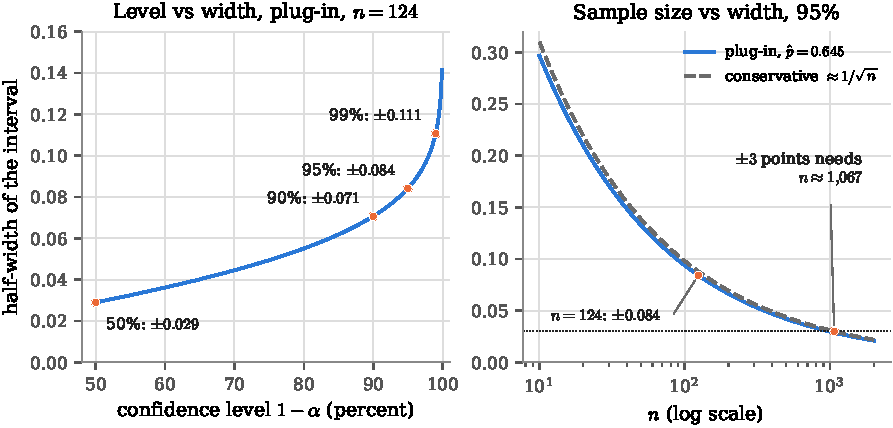
\includegraphics[width=\textwidth]{fig_ci_width}
\caption{Left: the half-width of the plug-in interval at $\hat{p} = 0.645$, $n = 124$, against the confidence level, with orange dots at the usual levels. Right: the half-width at $95\%$ against $n$, plug-in at $\hat{p} = 0.645$ (blue) and conservative (gray dashes).}
\label{fig:ciwidth}
\end{figure}

\textbf{The level.}
Raising the confidence level widens the interval, through the quantile, and the cost accelerates (\cref{fig:ciwidth}, left).
The quantile $q_{\alpha/2}$ does the work: $0.67$ at $50\%$, $1.645$ at $90\%$, $1.96$ at $95\%$, $2.58$ at $99\%$, $3.29$ at $99.9\%$, and infinite at $100\%$.
Going from $90\%$ to $95\%$ costs $19\%$ more width; from $95\%$ to $99\%$, $31\%$ more; and $100\%$ confidence costs the whole parameter space, since $q_{\alpha/2} \to \infty$ as $\alpha \to 0$.
This is why $95\%$ is a convention and not a law: it is a point on a curve where the interval is still informative and the miss rate is still small.
A $98\%$ interval of the same type always contains the $95\%$ one because $q_{0.01} > q_{0.025}$; but a $98\%$ interval need not contain a $95\%$ interval built differently. $[0, \, \bar{R}_n + q_{0.02}\,\widehat{\sigma}/\sqrt{n}]$ has asymptotic level $98\%$ and does not contain the $95\%$ lower-bound interval $[\bar{R}_n - q_{0.05}\,\widehat{\sigma}/\sqrt{n}, \, 1]$, nor the other way around: the $98\%$ interval reaches down to $0$ but stops short of $1$, the $95\%$ one reaches up to $1$ but stops short of $0$, so each contains points the other does not.
Nesting holds within one family of intervals indexed by $\alpha$, not between two intervals of different shapes whose levels happen to differ.

\textbf{The sample size.}
The width shrinks like $1/\sqrt{n}$ (\cref{fig:ciwidth}, right), which is the rate of the CLT and the rate of every interval in this book built from a sample mean.
Both curves on the right fall at that rate, the plug-in half-width at $\hat{p} = 0.645$ and the conservative half-width $q_{0.025}/(2\sqrt{n}) = 0.98/\sqrt{n}$, which is the pollster's `about $1/\sqrt{n}$'; the marked point is the $n \approx 1{,}067$ that a margin of $\pm 3$ points needs.
The practical form of $1/\sqrt{n}$: to halve the width you need four times the data; to get one more decimal place you need a hundred times the data.
Intervals that shrink faster exist when the model has special structure (\cref{ex:ci-shifted-expo} has one that shrinks like $1/n$), but they are built on the model's exact distribution rather than on the CLT, and they are fragile when the model is wrong.

\begin{bridge}[the pollster's $\pm 3$ points]
National polls report a `margin of error of $\pm 3$ percentage points' with about $1{,}000$ respondents, whatever the question.
That is the conservative interval: its half-width $q_{0.025}/(2\sqrt{n}) = 0.98/\sqrt{n} \approx 1/\sqrt{n}$ doesn't depend on $p$, so a pollster can state it before seeing a single answer.
Setting $0.98/\sqrt{n} = 0.03$ gives $n = (1.96/0.06)^2 = 1{,}067$.
The same arithmetic plans any proportion study: the sample size for a margin $m$ at $95\%$ is $n = (0.98/m)^2$, and the conservative bound is the right one to use because at the planning stage there is no $\hat{p}$ to plug in.
\end{bridge}

\section{What the \texorpdfstring{$95\%$}{95\%} means, and three things it doesn't}
\label{sec:ci-meaning}

Take $\mathcal{I}_{\text{plug-in}} = [0.12, 0.20]$ for the subway rate.
The sentence `$[0.12, 0.20]$ is a confidence interval of asymptotic level $95\%$ for $\lambda$' means: \textit{if you were to repeat the experiment}, collecting $64$ new inter-arrival times and computing the interval each time, the parameter $\lambda$ would be inside the resulting interval about $95\%$ of the time, with the approximation improving as $n$ grows.
This is the frequentist interpretation, and \cref{fig:cirepeated} is a hundred such repetitions.
Three readings that sound the same and are not:

\begin{pitfall}[three wrong readings]
\begin{enumerate}[nosep]
\item \textit{`The probability that $\lambda \in [0.12, 0.20]$ is $0.95$.'} No. $\lambda$ is a fixed number and $[0.12, 0.20]$ is a fixed interval; $\Pr(\lambda \in [0.12, 0.20])$ is $1$ or $0$, and the theory doesn't tell you which. The $0.95$ belongs to the procedure. (The sentence `you are $95\%$ confident that $\lambda$ is in $[0.12, 0.20]$', as in the drug example of \cref{ch:kiss}, is the accepted shorthand for the procedure statement, and is fine as long as it's read that way.)
\item \textit{`$95\%$ of the inter-arrival times fall in $[0.12, 0.20]$.'} No. The interval is for the parameter $\lambda$, not for the data; it shrinks to a point as $n \to \infty$ while the data's spread stays what it is.
\item \textit{`$95\%$ of the future estimates $\hat{\lambda}$ will fall in $[0.12, 0.20]$.'} No. A future $\hat{\lambda}$ is centered at $\lambda$, not at this sample's $0.16$, and lands in this particular interval about $95\%$ of the time only if this sample's $0.16$ happens to be close to $\lambda$, and less the further it is off.
\end{enumerate}
\end{pitfall}

The first reading is the one everyone wants, a probability statement about the parameter given the data.
It is available, but at a price: you must treat $\lambda$ as random, with a distribution before the data (a prior), and compute its distribution after the data (the posterior).
That is the Bayesian approach of \cref{ch:bayes-intro}, and the interval it produces, which \cref{ch:jeffreys} calls a Bayesian confidence region, does carry the probability $0.95$ in the sense of reading 1.
For large $n$ the two kinds of interval nearly coincide, which is the Bernstein--von Mises result mentioned in \cref{sec:conv-where-used}; what differs is what the number $0.95$ is a probability \textit{of}.

\section{What comes next}
\label{sec:ci-next}

A confidence interval answers `which values of $\theta$ are compatible with the data?'.
A test answers a narrower question, `is this particular value compatible?', and \cref{ex:ci-onesided} already showed that the two are the same construction: the value $\frac12$ is rejected exactly when it falls outside a one-sided interval.
\Cref{ch:tests-foundations} starts from the decision rather than the interval, which brings in two new things the interval didn't need: two kinds of error, with a level for one and a power for the other, and the $p$-value, which reports a test without fixing $\alpha$ in advance.
The thresholds $72$ and $74$ that \cref{ch:kiss} quoted are derived there.

\section{Summary}
\label{sec:ci-summary}

\begin{itemize}[nosep]
\item A confidence interval of level $1 - \alpha$ is a random interval with computable endpoints such that $\Pr_\theta(\mathcal{I} \ni \theta) \geq 1 - \alpha$ for every $\theta$; asymptotic level replaces the probability by its limit. Level is a floor: a $95\%$ interval is also a $90\%$ one.
\item The recipe: find a pivot, trap it between quantiles ($q_{\alpha/2}$ two-sided, $q_\alpha$ one-sided), solve for the parameter. Gaussian data with known variance give an exact pivot and an exact interval; the CLT gives an asymptotic pivot and an asymptotic interval.
\item When the pivot's scale involves the parameter, the interval it suggests isn't computable. Three fixes: bound the scale (conservative, level $\geq 1 - \alpha$, widest), solve the inequality for the parameter (solve, exact asymptotic level, one approximation), or estimate the scale and invoke Slutsky (plug-in, exact asymptotic level, two approximations). In the inversion picture they read the widest band, the lens, and a band of constant width.
\item Kiss experiment, $95\%$: conservative $[0.557, 0.733]$, solve $[0.558, 0.724]$, plug-in $[0.561, 0.729]$; they agree to within a point, and here the solve interval is the narrowest, not the widest. Subway: solve $[0.13, 0.21]$, plug-in $[0.12, 0.20]$, no conservative interval.
\item At finite $n$ the three behave differently: for a proportion the exact coverage can be computed from the Binomial, and at $n = 124$ the plug-in interval covers $0.939$ and the solve interval $0.952$ at $p = 0.645$, while at $n = 20$ the plug-in interval fails near the edges and the solve interval holds. Use solve for a proportion, plug-in otherwise.
\item A continuous, strictly monotone map carries a confidence interval for $\theta$ to one for $g(\theta)$ with the same level; the subway solve interval is the plug-in interval for $1/\lambda$ mapped through $x \mapsto 1/x$.
\item Half-width $= q_{\alpha/2} \, \widehat{\sigma}/\sqrt{n}$: the level acts through the quantile (and $100\%$ costs everything), the sample size through $1/\sqrt{n}$ (four times the data, half the width; $\pm 3$ points needs about $1{,}000$).
\item The level is the long-run hit rate of the procedure. A realized interval has no probability attached; the statement `$\Pr(p \in [0.56, 0.73]) = 0.95$' is Bayesian, and \cref{ch:bayes-intro} says what it costs.
\end{itemize}

\section{Exercises}
\label{sec:ci-exercises}

\begin{exercise}
\label{ex:ci-ninetyeight}
For the kiss data, find a $98\%$ asymptotic confidence interval for $p$ of the conservative and of the plug-in type. If $[0.34, 0.57]$ is a $95\%$ confidence interval for some proportion, is it also a $98\%$ one? A $90\%$ one?
\end{exercise}
\begin{solution}
$q_{0.01} = 2.326$. Conservative: the half-width is $2.326/(2\sqrt{124}) = 0.1045$, so $0.6452 \pm 0.1045 = [0.541, 0.750]$. Plug-in: the half-width is $2.326 \times 0.0430 = 0.1000$, so $0.6452 \pm 0.1000 = [0.545, 0.745]$. Both contain their $95\%$ versions, as they must for intervals of the same type. A $95\%$ interval is a $90\%$ interval (level is a floor) but is not in general a $98\%$ interval, so the answers are No to the $98\%$ question and Yes to the $90\%$ one.
\end{solution}

\begin{exercise}
\label{ex:ci-fifty}
A second study observes $150$ couples, $75$ turning each way, so $\bar{R}_n = 0.5$. Which of the following are realizations of $50\%$ asymptotic confidence intervals for $p$: (1) $[0, 0.5]$; (2) $[0.5, 1]$; (3) $[0.466, 0.533]$; (4) $[0.48, 0.52]$?
\end{exercise}
\begin{solution}
(1) is the realization of $[0, \bar{R}_n]$, and $\Pr_p([0, \bar{R}_n] \ni p) = \Pr_p(\bar{R}_n \geq p) \to \Pr(Z \geq 0) = \frac12$ for every $p$, by the CLT: a $50\%$ asymptotic interval, a strange one. (2) is $[\bar{R}_n, 1]$, the same argument. (3) is the realization at $n = 150$ of the rule $\bar{R}_n \pm c/\sqrt{n}$ with $c = 0.0335\sqrt{150} = 0.41$ (a fixed half-width would have limiting coverage $1$, so the rule has to shrink with $n$), and the conservative bound gives $\limn \Pr_p(\abs{\bar{R}_n - p} \leq c/\sqrt{n}) \geq \Pr(\abs{Z} \leq 2c) = \Pr(\abs{Z} \leq 0.82) = 0.59 \geq 0.5$ for every $p$: yes. (4) is the rule $\bar{R}_n \pm c/\sqrt{n}$ with $c = 0.02\sqrt{150} = 0.245$, and at $p = \frac12$ its limiting coverage is $\Pr(\abs{Z} \leq 2c) = \Pr(\abs{Z} \leq 0.49) = 0.38 < 0.5$. The definition asks for coverage at every $p$, and $p = \frac12$ is a $p$, so (4) is not a $50\%$ interval even though it is one for $p$ far from $\frac12$. The realizations of $50\%$ asymptotic intervals are therefore (1), (2) and (3).
\end{solution}

\begin{exercise}
\label{ex:ci-nesting}
Prove that $\mathcal{I}_{\text{plug-in}} \subseteq \mathcal{I}_{\text{conserv}}$ always, and find the sample for which the two coincide. Then show that $\mathcal{I}_{\text{solve}} = \mathcal{I}_{\text{plug-in}}$ never happens unless $\bar{R}_n = \frac12$, by comparing centers.
\end{exercise}
\begin{solution}
$\hat{p}(1 - \hat{p}) \leq \frac14$ for every $\hat{p} \in [0,1]$, so the plug-in half-width $q_{\alpha/2}\sqrt{\hat{p}(1-\hat{p})/n}$ is at most the conservative one $q_{\alpha/2}/(2\sqrt{n})$, with equality exactly when $\hat{p} = \frac12$. From \cref{eq:wilson}, the center of $\mathcal{I}_{\text{solve}}$ is $(\bar{R}_n + q_{\alpha/2}^2/(2n))/(1 + q_{\alpha/2}^2/n)$, which equals $\bar{R}_n$, the center of $\mathcal{I}_{\text{plug-in}}$, if and only if $\bar{R}_n + q^2/(2n) = \bar{R}_n + \bar{R}_n q^2/n$, that is, $\bar{R}_n = \frac12$. Otherwise the solve interval's center lies strictly between $\bar{R}_n$ and $\frac12$.
\end{solution}

\begin{exercise}
\label{ex:ci-curved}
Let $\Xton \iid \Gauss(\theta, \theta)$ for an unknown $\theta > 0$: the mean and the variance are the same unknown number. (a) Find an exact pivot based on $\bar{X}_n$. (b) Write the interval $\mathcal{I}_\theta$, depending on $\theta$, with exact coverage $90\%$. (c) Find the plug-in interval of asymptotic level $90\%$. (d) Find the solve interval, and say whether its level is exact or asymptotic.
\end{exercise}
\begin{solution}
(a) $\bar{X}_n \sim \Gauss(\theta, \theta/n)$ exactly, so $\sqrt{n/\theta}\,(\bar{X}_n - \theta) \sim \Gauss(0,1)$ for every $n$ and $\theta$. (b) With $t = q_{0.05} = 1.645$: $\mathcal{I}_\theta = [\bar{X}_n - t\sqrt{\theta/n}, \; \bar{X}_n + t\sqrt{\theta/n}]$, exact coverage $0.90$, not computable. (c) $\bar{X}_n \convp \theta$, so Slutsky gives $\sqrt{n/\bar{X}_n}\,(\bar{X}_n - \theta) \convd \Gauss(0,1)$ and $\mathcal{I}_{\text{plug-in}} = \bar{X}_n \pm t\sqrt{\bar{X}_n/n}$, asymptotic level $90\%$. (d) $\frac{n}{\theta}(\bar{X}_n - \theta)^2 \leq t^2$ is $\theta^2 - (2\bar{X}_n + t^2/n)\theta + \bar{X}_n^2 \leq 0$, so
\[
\mathcal{I}_{\text{solve}} = \left[ \bar{X}_n + \frac{t^2}{2n} - \sqrt{\Delta}, \; \bar{X}_n + \frac{t^2}{2n} + \sqrt{\Delta} \right], \qquad \Delta = \frac{t^4}{4n^2} + \frac{t^2 \bar{X}_n}{n}.
\]
Because the pivot in (a) is exact, so is this interval's level: it is a confidence interval of level $90\%$ for every $n$, not only asymptotically. Solving adds no approximation beyond the pivot's own; plugging in always adds one.
\end{solution}

\begin{exercise}
\label{ex:ci-shifted-expo}
Let $\Xton$ be i.i.d.\ with density $f(x) = e^{-(x - a)} \ind(x \geq a)$, a unit Exponential shifted by an unknown $a \in \real$. (a) Show that $\hat{a}_1 = \bar{X}_n - 1$ is consistent and find its asymptotic distribution and the two-sided plug-in interval of asymptotic level $1 - \alpha$. (b) Let $\hat{a}_2 = \min_i X_i$. Show that $n(\hat{a}_2 - a) \sim \Expo(1)$ exactly, and build a one-sided interval of exact level $1 - \alpha$ from it. (c) Compare the two intervals' widths and their robustness.
\end{exercise}
\begin{solution}
(a) $\E[X_1] = a + 1$ and $\var(X_1) = 1$ (a shift doesn't change the variance of $\Expo(1)$), so $\hat{a}_1 \convp a$ by the LLN and $\sqrt{n}(\hat{a}_1 - a) \convd \Gauss(0,1)$ by the CLT. The asymptotic variance is known, so there is nothing to plug in: $\mathcal{I}_1 = \hat{a}_1 \pm q_{\alpha/2}/\sqrt{n}$. (b) For $t \geq a$, $\Pr(\hat{a}_2 > t) = \Pr(X_i > t \ \forall i) = (e^{-(t-a)})^n = e^{-n(t-a)}$, so $\Pr(n(\hat{a}_2 - a) > s) = e^{-s}$: $n(\hat{a}_2 - a) \sim \Expo(1)$, for every $n$. Since $\hat{a}_2 \geq a$ always, the natural interval is $[\hat{a}_2 - s, \hat{a}_2]$, and $\Pr(a \in [\hat{a}_2 - s, \hat{a}_2]) = \Pr(n(\hat{a}_2 - a) \leq ns) = 1 - e^{-ns}$. Setting this to $1 - \alpha$ gives $s = \log(1/\alpha)/n$ and $\mathcal{I}_2 = [\hat{a}_2 - \log(1/\alpha)/n, \; \hat{a}_2]$, exact level $1 - \alpha$. (c) $\mathcal{I}_1$ has width $2q_{\alpha/2}/\sqrt{n}$ and $\mathcal{I}_2$ has width $\log(1/\alpha)/n$: at $n = 100$ and $\alpha = 0.05$, $0.39$ against $0.03$. The minimum is tailored to the model, uses its exact distribution, and needs no asymptotics. It is also fragile: one observation below $a$, impossible under the model but possible under a slightly wrong one, breaks it completely, while the sample mean barely notices. The generic $1/\sqrt{n}$ interval is the price of robustness.
\end{solution}

\begin{exercise}
\label{ex:ci-onesided}
For the kiss data, build a $95\%$ lower confidence bound for $p$ of the plug-in type and of the conservative type. Then show that `$\frac12$ is below the conservative lower bound' is the same event as `$n\bar{R}_n \geq 72$', the one-sided threshold that \cref{ch:kiss} quoted and \cref{ch:tests-foundations} derives.
\end{exercise}
\begin{solution}
One-sided, so $q_{0.05} = 1.645$. Plug-in: $[0.645 - 1.645 \times 0.0430, \, 1] = [0.574, 1]$. Conservative: $[0.645 - 1.645/(2\sqrt{124}), \, 1] = [0.571, 1]$. With $95\%$ confidence, at least $57\%$ of couples turn right. The conservative lower bound exceeds $\frac12$ when $\bar{R}_n - 1.645/(2\sqrt{n}) > \frac12$, that is, $\bar{R}_n > 0.5 + 0.0739 = 0.5739$, that is, $n\bar{R}_n > 71.2$, that is, $n\bar{R}_n \geq 72$. A confidence interval excluding the value $\frac12$ and a test rejecting $p = \frac12$ are the same decision looked at from two sides, and the conservative scale $\frac12$ is exactly the scale the test uses under its null hypothesis; \cref{ch:tests-foundations} makes this duality general.
\end{solution}

\begin{exercise}
\label{ex:ci-gamma}
The subway data have an exact interval that uses no limit theorem. If $T_1, \ldots, T_n \iid \Expo(\lambda)$ then $\lambda \sum_i T_i = \lambda n \bar{T}_n$ has the Gamma distribution with shape $n$ and rate $1$, whatever $\lambda$ is (you may take this as given). Use it as a pivot to build a confidence interval for $\lambda$ of exact level $95\%$, and compute it for $n = 64$, $\bar{T}_n = 6.23$, given that the $2.5\%$ and $97.5\%$ points of that Gamma distribution are $49.29$ and $80.60$.
\end{exercise}
\begin{solution}
The pivot is $G = \lambda n \bar{T}_n$, whose distribution doesn't involve $\lambda$. Trap it: $\Pr(49.29 \leq \lambda n \bar{T}_n \leq 80.60) = 0.95$ for every $\lambda$ and this $n$. Solve for $\lambda$: $\lambda \in [49.29/(n\bar{T}_n), \, 80.60/(n\bar{T}_n)]$, an interval of exact level $95\%$ with computable endpoints. With $n\bar{T}_n = 398.7$: $[0.124, 0.202]$, between the solve interval $[0.129, 0.213]$ and the plug-in interval $[0.121, 0.200]$ of \cref{sec:ci-subway}, and like the solve interval not centered at $\hat{\lambda} = 0.1605$. This is the exact interval \cref{sec:conv-what-limits-buy} mentioned; it exists because the parent distribution is known in full, which is exactly what the CLT lets you do without.
\end{solution}

\chapter[Hypothesis Tests]{Hypothesis Tests: Errors, Level, Power and $p$-Values}
\label{ch:tests-foundations}

\begin{chaptergoals}
\begin{itemize}[nosep]
\item What a test is: a yes/no rule applied to the data, written as an indicator of a rejection region. The null hypothesis is the claim the data are allowed to overturn; the alternative is what you conclude when they do.
\item The two ways a test can be wrong, why they are not treated alike, and the two numbers that describe a test: its level, a cap on one error, and its power, one minus the other.
\item The recipe behind every test in this book: a test statistic whose distribution under the null hypothesis you know, and a quantile of that distribution as the threshold. One-sided and two-sided versions, and why the null hypothesis makes the unknown parameter known.
\item The test for the kiss data, done exactly and done by the CLT: thresholds $72$ and $74$ one way, $72$ and $73$ the other, and why they differ.
\item The $p$-value: the smallest level at which the data reject, and the one number a test reports.
\item Tests and confidence intervals are the same construction seen from two sides.
\end{itemize}
The running example is the kiss experiment: $n = 124$ couples, $80$ turning right, and the question \cref{ch:kiss} opened with, whether $80$ is more than chance would produce if couples had no preference for either side.
\end{chaptergoals}

\section{A yes/no question about a parameter}
\label{sec:tests-question}

A confidence interval reports a range.
Often what is wanted is a decision.
The examples below are the kind a manager or a scientist actually faces, and each is a yes/no question about a parameter of a model.

\begin{itemize}
\item \textbf{Boarding a plane.} Two airlines board differently: one from the rear of the plane to the front (`R2F'), the other by window seats first, then middle, then aisle (`WilMA').
Which is faster?
The data are $n = 72$ R2F flights averaging $24.2$ minutes with a standard deviation of $2.1$, and $m = 56$ WilMA flights averaging $15.9$ minutes with a standard deviation of $1.3$.
With boarding times modeled as $X \sim \Gauss(\mu_1, \sigma_1^2)$ and $Y \sim \Gauss(\mu_2, \sigma_2^2)$ and the two samples independent, the question is: is $\mu_1 = \mu_2$, or is $\mu_1 > \mu_2$?
Two samples, one question: a \textbf{two-sample test}.
\item \textbf{Waiting in the emergency room.} The national average wait is $30$ minutes.
Patients at one hospital say its wait is longer.
With $\Xton$ the waits of $n$ random patients there and $\mu = \E[X_1]$, the question is: is $\mu > 30$?
One sample: a \textbf{one-sample test}.
\item \textbf{The kiss experiment.} If couples have no preference for either side, $p = \frac12$.
Of $124$ couples, $80$ turned right.
Is $p = \frac12$, or not?
\end{itemize}

The obvious first answer to the boarding question is `$\bar{X}_n = 24.2 > 15.9 = \bar{Y}_m$, so $\mu_1 > \mu_2$'.
What is wrong with it is this: by bad luck the $72$ R2F flights might all have been full and the $56$ WilMA flights half empty, and sample means move from sample to sample.
A better rule puts a buffer around each mean and asks whether the buffers still separate:
\[
\text{conclude } \mu_1 > \mu_2 \text{ if } \bar{X}_n - \text{buffer} > \bar{Y}_m + \text{buffer}.
\]
For the one-sample version, conclude $\mu > 30$ if $\bar{X}_n > 30 + \text{buffer}$.
What should the buffer be?
Something that measures the size of the random fluctuations of $\bar{X}_n$, and \cref{ch:clt} says what that is: a few multiples of $\sigma/\sqrt{n}$.
\Cref{fig:testbuffer} draws the heuristic for the boarding data and for two one-sample examples, with a buffer of two standard errors around each estimate.
With $n = 72$ and $m = 56$ the buffers around $24.2$ and $15.9$ minutes reach about half a minute (R2F) and a third of a minute (WilMA) on each side, nowhere near each other, and the conclusion is not in doubt.
For a coin tossed $30$ times with $13$ heads, the buffer $0.43 \pm 0.18$ reaches well past $\frac12$, and the heuristic says nothing.
For a survey of $4{,}971$ Americans in which $32\%$ get news on YouTube, the buffer $0.32 \pm 0.013$ just reaches the $33\%$ being tested, and again the heuristic is silent.
For a proportion the buffer is $2\sqrt{\hat{p}(1-\hat{p})/n}$, and it shrinks like $1/\sqrt{n}$.

\begin{figure}[htbp]
\centering
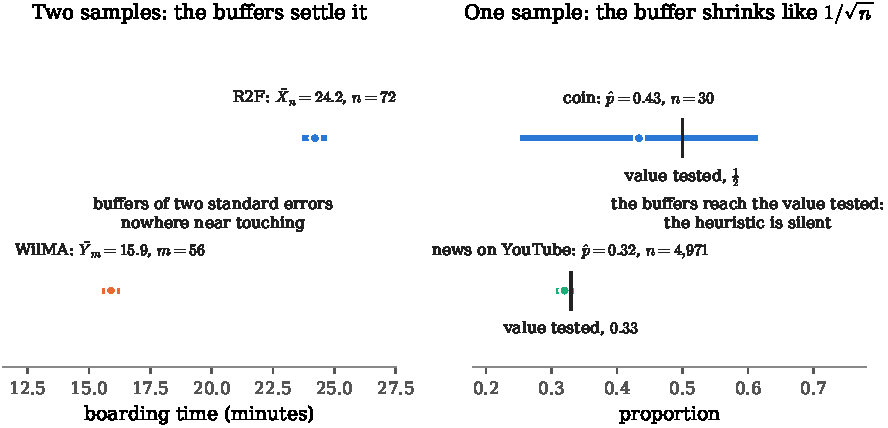
\includegraphics[width=\textwidth]{fig_test_buffer}
\caption{Buffers of two standard errors around each estimate (dot). Left: the boarding data, R2F (blue) and WilMA (orange). Right: two one-sample proportions, the coin (blue) and the YouTube survey (aqua), each with the value being tested as a black tick.}
\label{fig:testbuffer}
\end{figure}

The rest of the chapter makes the heuristic precise: what counts as a buffer, what guarantee it comes with, and what to report when the data land near the edge.

\begin{bridge}[statistically significant]
Every one of these questions was answered in an introductory course with a $z$-test or a $t$-test and the phrase `the difference is statistically significant at the $5\%$ level'.
This chapter is that procedure, written so that each piece has a name and a guarantee: the hypotheses, the rejection region, the two errors, the level, the power and the $p$-value.
`Significant at $5\%$' will turn out to mean `the test of level $5\%$ rejected', and `$p < 0.05$' will be a theorem rather than a rule of thumb.
\end{bridge}

\section{Null and alternative hypotheses}
\label{sec:tests-hypotheses}

Let $\Xton$ be a sample of i.i.d.\ r.v.s and $\statmodel$ a statistical model (\cref{ch:models}).
Let $\Theta_0$ and $\Theta_1$ be disjoint subsets of $\Theta$.
The two hypotheses are
\[
H_0: \theta \in \Theta_0 \qquad \text{and} \qquad H_1: \theta \in \Theta_1.
\]
$H_0$ is the \textbf{null hypothesis}, $H_1$ the \textbf{alternative hypothesis}.
If you believe the true $\theta$ is in one of the two sets, you test $H_0$ against $H_1$: you look in the data for evidence against $H_0$, and you decide whether to \textbf{reject} $H_0$.\footnote{Some treatments require $\Theta_0$ and $\Theta_1$ to partition $\Theta$, and others, this book among them, ask only that the two sets be disjoint. The difference matters when values of $\theta$ in neither set are possible, in which case the test is silent about them. In every example in this book the two sets partition $\Theta$.}

The two hypotheses do not play symmetric roles, and this asymmetry is the first thing to internalize.
The data are used only to try to disprove $H_0$.
If they fail to, that is not evidence that $H_0$ is true; it is a lack of evidence against it.
The standard phrase is `innocent until proven guilty': the null hypothesis is the defendant, the data are the evidence, and a verdict of not guilty is not a finding of innocence.
So the conclusions of a test are `reject $H_0$' and `fail to reject $H_0$', never `accept $H_0$'.

Which claim goes in the null?
The one that gets the benefit of the doubt: the status quo, the claim of no effect, the value you would act on if the data said nothing.
For the kiss experiment the null is $p = \frac12$, no preference; for the emergency room it is `the wait is not longer than the national average'; for the boarding methods it is `no difference'.
The alternative is the claim that needs evidence to be adopted, and it is the one the study was run to look for.

\textbf{Simple and composite.}
A hypothesis is \textbf{simple} if its set is a single point, $\Theta_k = \{\theta_k\}$, and \textbf{composite} otherwise, typically a half-line $\{\theta > \theta_k\}$ or $\{\theta < \theta_k\}$ or everything but a point, $\{\theta \neq \theta_k\}$.
When $\Theta \subseteq \real$ and $H_0$ is simple, $H_0: \theta = \theta_0$, the terminology is:
\begin{itemize}[nosep]
\item \textbf{two-sided test}: $H_1: \theta \neq \theta_0$, departures in either direction count as evidence;
\item \textbf{one-sided test}: $H_1: \theta > \theta_0$ or $H_1: \theta < \theta_0$, only one direction counts.
\end{itemize}
One-sided tests are also written with a composite null, $H_0: \theta \leq \theta_0$ against $H_1: \theta > \theta_0$; \cref{sec:tests-errors} explains why the two forms of the null lead to the same test.
For the examples above: the boarding question is one-sided ($\mu_1 > \mu_2$); the emergency room is one-sided ($\mu > 30$); the fair coin is two-sided ($p \neq \frac12$); and the test for the kiss data can be put either way, two-sided as $H_0: p = \frac12$ against $H_1: p \neq \frac12$, or one-sided as \cref{ch:kiss} asked it, $H_1: p > \frac12$.
Both are done below.

\begin{pitfall}[one-sided is a modeling decision, not a reading of the data]
Writing $H_1: \mu_1 > \mu_2$ for the boarding methods says that $\mu_1 < \mu_2$ is not a possibility you entertain.
The modeling assumption reduces the number of ways the hypothesis $\mu_1 = \mu_2$ can be rejected: $\mu_1 < \mu_2$ is not allowed, so a sample pointing that way counts as no evidence against the null at all.
That decision has to be made before looking at the data.
Choosing the side after seeing which way $\bar{X}_n - \bar{Y}_m$ came out is a way of rejecting more often than the level promises: a nominal $5\%$ becomes an actual $10\%$, since a two-sided question is then being answered with a one-sided threshold.
\Cref{sec:tests-kiss} shows the thresholds differ ($72$ against $74$ right turns for the kiss data), which is exactly the room this mistake exploits.
\end{pitfall}

\section{What a test is}
\label{sec:tests-definition}

\begin{definition}[Test, rejection region]
\label{def:test}
A \textbf{test} is a statistic $\psi: E^n \to \{0, 1\}$: a function of the sample $\Xton$ taking the values $0$ and $1$, such that
\begin{itemize}[nosep]
\item if $\psi(\Xton) = 0$, $H_0$ is not rejected;
\item if $\psi(\Xton) = 1$, $H_0$ is rejected.
\end{itemize}
The \textbf{rejection region} of $\psi$ is the set of samples on which it rejects,
\[
R_\psi = \{ (x_1, \ldots, x_n) \in E^n : \psi(x_1, \ldots, x_n) = 1 \},
\]
so that $\psi = \ind(R_\psi)$ \toolkit{sec:math-indicator}.
\end{definition}

\begin{inwords}
\textbf{In words.} A test is a rule, fixed before the data arrive, that sorts every possible sample into two bins: reject or don't. The rejection region is the `reject' bin, and the test is its indicator. Because the rule is applied to a random sample, $\psi$ is a random variable, a Bernoulli one, and asking how often it equals $1$ is a probability question, like asking how often an interval covers.
\par\smallskip
\textbf{For the kiss data.} `Reject $p = \frac12$ if $72$ or more of the $124$ couples turn right' is the test $\psi = \ind(n\bar{R}_n \geq 72)$. Its rejection region is every sequence of $124$ zeros and ones with at least $72$ ones. On the sample we have, $n\bar{R}_n = 80$ and $\psi = 1$.
\end{inwords}

The definition contains no probability: a test is a partition of the sample space $E^n$ of \cref{sec:models-sample-space} into two pieces.
Probability enters when you ask how the test behaves under each candidate $\Pr_\theta$, which is the next section.

In practice every test in this book has the form
\[
\psi = \ind( T_n > c )
\]
for a statistic $T_n = T_n(\Xton)$, called the \textbf{test statistic}, and a number $c$, the \textbf{threshold}; the rejection region is then $\{T_n > c\}$ (for a count, `$\geq 72$' is `$> 71$', so the strict inequality is only a matter of where $c$ sits).
The test statistic compresses the sample into one number that measures how far the data are from what $H_0$ predicts, and the threshold says how far is too far.
Everything a test does is in those two choices, and the sections that follow are about making them.

\begin{bridge}[the test statistic you already know]
In an introductory course the test statistic was $z = (\bar{x} - \mu_0)/(\sigma/\sqrt{n})$, or $t$ with $s$ in place of $\sigma$, and the threshold was a number from a table, $1.96$ or $1.645$ or a $t$ critical value.
That is $\psi = \ind(\abs{T_n} > c)$ with $T_n$ the standardized mean.
What this chapter adds is the function $\psi$ itself as an object, so that `the test rejects with probability $\alpha$ when $H_0$ is true' is a statement about a random variable with a definition, and so that tests with other statistics (likelihood ratios in \cref{ch:wald-lrt}, chi-squared distances in \cref{ch:gof}) are the same object with a different $T_n$.
\end{bridge}

\section{Two kinds of error, level and power}
\label{sec:tests-errors}

A test can be wrong in two ways, and the standard table lays them out with the truth in the rows and the decision in the columns:
\begin{center}
\begin{tabular}{@{}lcc@{}}
\toprule
 & not rejected ($\psi = 0$) & rejected ($\psi = 1$) \\
\midrule
$H_0$ true ($\theta \in \Theta_0$) & correct & \textbf{type 1 error} \\
$H_1$ true ($\theta \in \Theta_1$) & \textbf{type 2 error} & correct \\
\bottomrule
\end{tabular}
\end{center}
A \textbf{type 1 error} is rejecting $H_0$ when it is true: convicting the innocent.
A \textbf{type 2 error} is failing to reject $H_0$ when $H_1$ is true: acquitting the guilty.
Since the truth is one fixed $\theta$ and the decision is random, the natural measure of each error is a probability, and since the probability depends on which $\theta$ is true, each error is a \textit{function} of $\theta$ on its own hypothesis.

\begin{definition}[Type 1 error, type 2 error, power]
\label{def:errors}
For a test $\psi$ of $H_0: \theta \in \Theta_0$ against $H_1: \theta \in \Theta_1$:
\begin{itemize}[nosep]
\item the \textbf{type 1 error} of $\psi$ is the function
\[
\alpha_\psi: \Theta_0 \to [0, 1], \qquad \theta \mapsto \Pr_\theta(\psi = 1);
\]
\item the \textbf{type 2 error} of $\psi$ is the function
\[
\beta_\psi: \Theta_1 \to [0, 1], \qquad \theta \mapsto \Pr_\theta(\psi = 0);
\]
\item the \textbf{power} of $\psi$ is the number \toolkit{sec:math-sup}
\[
\pi_\psi = \inf_{\theta \in \Theta_1} \left( 1 - \beta_\psi(\theta) \right).
\]
\end{itemize}
\end{definition}

\begin{inwords}
\textbf{In words.} Fix a truth $\theta$ and imagine rerunning the study many times. If $\theta$ is in the null set, the fraction of reruns on which the test rejects is the type 1 error at that $\theta$; if $\theta$ is in the alternative, the fraction on which it fails to reject is the type 2 error at that $\theta$, and the fraction on which it rejects is the power at that $\theta$. The power of the test is the worst case of that last fraction over the whole alternative: the least the test can be relied on to detect a departure from $H_0$.
\par\smallskip
\textbf{For the kiss data.} For $\psi = \ind(n\bar{R}_n \geq 72)$ and the one-sided hypotheses $H_0: p = \frac12$, $H_1: p > \frac12$: the type 1 error is the single number $\Pr_{1/2}(n\bar{R}_n \geq 72) = 0.044$. The type 2 error at $p = 0.645$ is $\Pr_{0.645}(n\bar{R}_n \leq 71) = 0.057$, so the test detects a true $p$ of $0.645$ with probability $0.943$. The power in the definition's sense is $\inf_{p > 1/2}$ of that detection probability, which is $0.044$, approached as $p \downarrow \frac12$: no test can reliably detect a $p$ just above $\frac12$ with $124$ couples, and the infimum records that.
\end{inwords}

\begin{figure}[htbp]
\centering
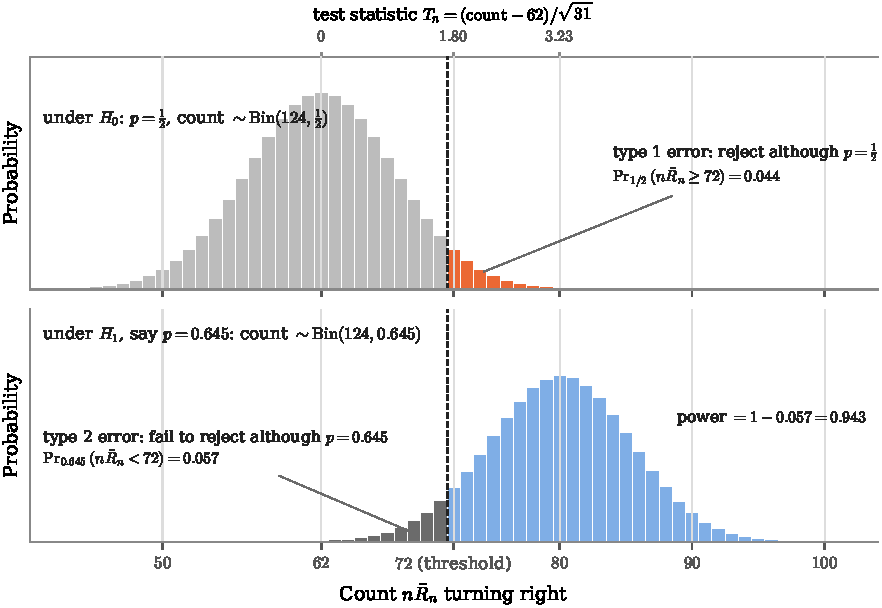
\includegraphics[width=\textwidth]{fig_test_two_errors}
\caption{The test `reject $p = \frac12$ if the count is $72$ or more', threshold dashed. Top: the count under $p = \frac12$, mass at $72$ and above in orange. Bottom: the count under $p = 0.645$, mass below $72$ in gray, the rest in blue.}
\label{fig:twoerrors}
\end{figure}

\Cref{fig:twoerrors} is the picture to hold on to.
The same threshold cuts two different distributions of the count: the one $H_0$ predicts and one of the many $H_1$ allows.
At the top, if $p = \frac12$ the count is $\mathrm{Bin}(124, \frac12)$, centered at $62$, and the orange mass at $72$ and above is the type 1 error, $0.044$.
At the bottom, if instead $p = 0.645$ the count is $\mathrm{Bin}(124, 0.645)$, centered at $80$; the gray mass below $72$ is the type 2 error at that $p$, $0.057$, and the blue mass is the power there, $0.943$.
What falls on the wrong side of the cut under each is the corresponding error.
The scale along the top of each is the test statistic $T_n = (\text{count} - 62)/\sqrt{31}$ of \cref{sec:tests-clt}: the threshold $72$ is $T_n = 1.80$, and the observed $80$ is $3.23$.
And the picture shows the trade: sliding the threshold to the right makes the type 1 error smaller and the type 2 error larger (the orange shrinks and the gray grows), sliding it left does the reverse, and at a fixed $n$ you cannot shrink both.
The two distributions pull apart as $n$ grows (their standard deviations are $\sqrt{p(1-p)/n}$ on the proportion scale), and that is the only lever that lowers both errors at once.

Rather than two functions on two sets, it is often clearer to look at one function on all of $\Theta$, the probability of rejecting,
\[
\theta \mapsto \Pr_\theta(\psi = 1),
\]
which is $\alpha_\psi$ on $\Theta_0$ and $1 - \beta_\psi$ on $\Theta_1$.\footnote{Two conventions for the letter $\beta$ are in common use. This book writes $\beta_\psi$ for the type 2 error, as in \cref{def:errors}. Elsewhere $\beta(\theta)$ names this rejection probability itself, the power function, which is $1 - \beta_\psi(\theta)$ on $\Theta_1$ and $\alpha_\psi(\theta)$ on $\Theta_0$. Check which one a source means before carrying a formula across.}
\Cref{fig:powercurve} draws it for the kiss data, computed exactly from the Binomial distribution of the count.
On the left, at $n = 124$, the one-sided test rejects for a count of $72$ or more and the two-sided test for $74$ or more or $50$ or fewer.
At $p = \frac12$ both curves are at or below $0.05$ (they are $0.044$ and $0.038$); to the right both climb to $1$, the one-sided test faster since it spends its whole $5\%$ on that side; to the left the two-sided test climbs and the one-sided test, which does not watch that side, stays at $0$.
On the right, the one-sided test at $n = 30$ (threshold $20$) sits beside the same test at $n = 124$: more data makes the curve steeper, so both errors fall at once.
A good test has a rejection curve that is low on $\Theta_0$ and climbs quickly to $1$ on $\Theta_1$; the level, defined next, caps the low part, and the power is the lowest point of the high part.

\begin{figure}[htbp]
\centering
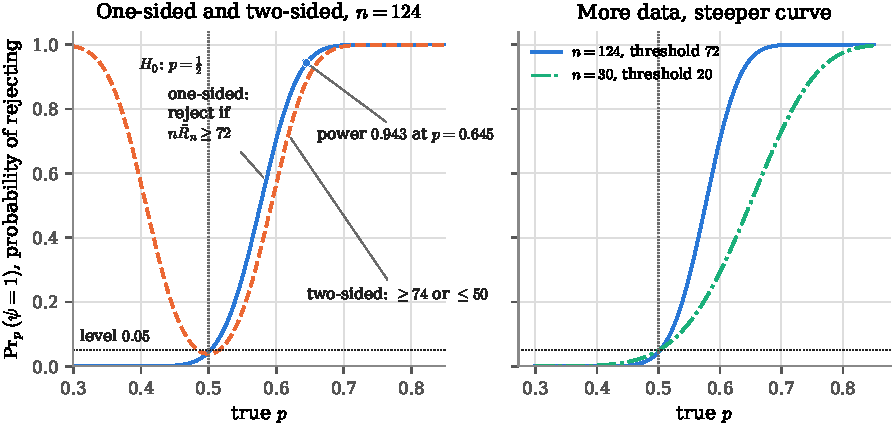
\includegraphics[width=\textwidth]{fig_power_curve}
\caption{The probability of rejecting against the true $p$, with the level $0.05$ dotted. Left, $n = 124$: one-sided, count $\geq 72$ (solid), and two-sided, $\geq 74$ or $\leq 50$ (dashed). Right: one-sided at $n = 124$ (solid) and $n = 30$ (dash-dot).}
\label{fig:powercurve}
\end{figure}

\begin{bridge}[$\alpha$, $\beta$ and the power calculation]
An introductory course calls the type 1 error probability $\alpha$ and the type 2 error probability $\beta$, says `power $= 1 - \beta$', and may have made you compute the sample size needed for $80\%$ power against a specific alternative.
All of that is here. The only addition is that $\alpha$ and $\beta$ are functions of $\theta$, not single numbers: a type 2 error of $0.057$ is a type 2 error \textit{at} $p = 0.645$, and at $p = 0.55$ the same test has a type 2 error of $0.72$, which is why failing to reject is not accepting: this test misses a true $p$ of $0.55$ nearly three times in four.
The power calculation of an introductory course picks one alternative and reads one point off \cref{fig:powercurve}'s curve; the power $\pi_\psi$ of \cref{def:errors} takes the infimum over all of them, which for a composite alternative that touches $\Theta_0$ is the rejection probability at the edge of $\Theta_0$, $0.044$ here: at most the level, and useless as a summary of what the test can detect. The one-point version is the useful one in planning a study, and the infimum is the one that describes the test over the whole alternative.
\end{bridge}

\begin{definition}[Level, asymptotic level]
\label{def:level}
Let $\alpha \in (0, 1)$.
A test $\psi$ has \textbf{level} $\alpha$ if
\[
\alpha_\psi(\theta) \leq \alpha \quad \text{for all } \theta \in \Theta_0,
\]
and \textbf{asymptotic level} $\alpha$ if
\[
\limn \alpha_{\psi_n}(\theta) \leq \alpha \quad \text{for all } \theta \in \Theta_0,
\]
where $\psi_n$ is the test built on $n$ observations \toolkit{sec:math-limits}.
\end{definition}

\begin{inwords}
\textbf{In words.} A test of level $5\%$ is one that convicts the innocent at most $5\%$ of the time, whichever innocent $\theta$ is the truth. The level is a cap on the worst case of the type 1 error over the whole null set, not the type 1 error at one point. `Asymptotic' means the cap is guaranteed only in the limit of large samples, which is what a CLT-based threshold delivers.
\par\smallskip
\textbf{For the kiss data.} $\psi = \ind(n\bar{R}_n \geq 72)$ has level $5\%$ for $H_0: p = \frac12$ exactly, since $0.044 \leq 0.05$; it also has level $5\%$ for the composite null $H_0: p \leq \frac12$, since $\Pr_p(n\bar{R}_n \geq 72)$ only decreases as $p$ falls below $\frac12$. The threshold $71$ would not do: $\Pr_{1/2}(n\bar{R}_n \geq 71) = 0.063$.
\end{inwords}

Two remarks on the definition, both consequences of the asymmetry of \cref{sec:tests-hypotheses}.
First, the level is a guarantee about the type 1 error only.
A test of level $5\%$ promises nothing about its type 2 error; $\psi \equiv 0$, the test that never rejects, has level $5\%$ (its type 1 error is $0$) and is useless.
The standard way of choosing a test is to fix the level first and then, among tests of that level, prefer the one with the most power.
Second, the level is a cap, so a test of level $5\%$ is also a test of level $10\%$: `level $5\%$' is a one-directional bound, as `level $95\%$' was for an interval in \cref{ch:confidence-intervals}, the worst the procedure can do rather than what it does.

\begin{pitfall}[level $\alpha$ for a test, level $1 - \alpha$ for an interval]
The same word, the same $\alpha$, complementary conventions.
For a confidence interval the level is $1 - \alpha$, the probability of a correct capture.
For a test the level is $\alpha$, the probability of an incorrect rejection.
Both conventions describe the procedure by the guarantee it gives, and the guarantee for a test is about the error it controls.
\Cref{sec:tests-duality} shows the two procedures are one object, which is why the same $\alpha$ appears in both.
\end{pitfall}

\begin{intuition}[why the worst case over $\Theta_0$]
For a one-sided question such as `can we conclude that at most a third of Americans get news on YouTube?' you would write $H_0: p \geq 0.33$ against $H_1: p < 0.33$, a composite null. Which $p$ in $\Theta_0$ should the threshold be computed from?
The definition answers: the one that makes rejection most likely, since the level must hold for every $p$ in $\Theta_0$.
The test rejects when $\hat{p}$ is small, and a small $\hat{p}$ is likeliest when $p$ is as small as $\Theta_0$ allows, that is, at the boundary $p = 0.33$.
So the composite null $p \geq 0.33$ is tested with the threshold of the simple null $p = 0.33$, and no separate computation is needed.
The same reasoning gives the threshold $72$ of the kiss data for $H_0: p \leq \frac12$.
This is why one-sided tests are freely written either way.
\end{intuition}

\section{Building a test from the Central Limit Theorem}
\label{sec:tests-clt}

The general-purpose test is the standardized mean, and, as in the plug-in interval of \cref{ch:confidence-intervals}, all three limit tools of Part II work together in its one argument.

Let $\Xton$ be i.i.d.\ with mean $\mu$ and variance $\sigma^2$, both finite, and let $\mu_0$ be a fixed number.
To test $H_0: \mu = \mu_0$ against $H_1: \mu \neq \mu_0$, take
\[
T_n = \sqrt{n}\, \frac{\bar{X}_n - \mu_0}{\sigma}.
\]
If $H_0$ is true then $\mu = \mu_0$ and the CLT (\cref{thm:clt}) says $T_n \convd \Gauss(0, 1)$.
So under $H_0$ the probability that $\abs{T_n}$ exceeds $q_{\alpha/2}$ tends to $\Pr(\abs{Z} > q_{\alpha/2}) = \alpha$, and the test
\[
\psi_\alpha = \ind( \abs{T_n} > q_{\alpha/2} )
\]
has asymptotic level $\alpha$.
The one-sided versions use one tail: for $H_1: \mu > \mu_0$, $\psi_\alpha = \ind(T_n > q_\alpha)$; for $H_1: \mu < \mu_0$, $\psi_\alpha = \ind(T_n < -q_\alpha)$.
\Cref{fig:gaussquantiles} in \cref{ch:gaussian} is the picture: $q_{\alpha/2}$ leaves $\alpha/2$ in each tail, $q_\alpha$ leaves $\alpha$ in one.

\begin{proposition}[The standardized-mean test]
\label{prop:clt-test}
Under the assumptions above, with $\sigma$ known or replaced by any consistent estimator $\hat{\sigma}_n$:
\begin{enumerate}[nosep]
\item $\psi_\alpha = \ind(\abs{T_n} > q_{\alpha/2})$ has asymptotic level $\alpha$ for $H_0: \mu = \mu_0$, and $\ind(T_n > q_\alpha)$ has asymptotic level $\alpha$ for $H_0: \mu \leq \mu_0$.
\item Under any $\mu \neq \mu_0$ in the alternative, $\Pr_\mu(\psi_\alpha = 1) \to 1$: the type 2 error at every fixed alternative tends to $0$.
\end{enumerate}
\end{proposition}

\coreproof{Under $H_0$ the CLT gives the limit of the rejection probability, and it is a limit of numbers, computed from $\Phi$. With $\hat{\sigma}_n$ in place of $\sigma$, Slutsky supplies the same limit. Under $H_1$ the LLN sends $\bar{X}_n - \mu_0$ to a nonzero constant, so $T_n$ runs off to $\pm\infty$.}
\begin{proof}
(1) Under $\Pr_{\mu_0}$, $T_n \convd Z \sim \Gauss(0,1)$ by the CLT, and the set $\{\abs{z} > q_{\alpha/2}\}$ has boundary points $\pm q_{\alpha/2}$ at which $Z$ has no mass, so convergence in distribution gives convergence of the probabilities (\cref{prop:convd-equiv}):
\[
\alpha_{\psi_n}(\mu_0) = \Pr_{\mu_0}(\abs{T_n} > q_{\alpha/2}) \to \Pr(\abs{Z} > q_{\alpha/2}) = \alpha.
\]
This is a limit of a sequence of numbers, one per $n$, and not a mode of convergence of random variables.
The random variable $T_n$ is the thing that converges in distribution; the probability it assigns to the fixed set $\{\abs{z} > q_{\alpha/2}\}$ is a number for each $n$, and those numbers converge in the ordinary calculus sense \toolkit{sec:math-limits}.
If $\sigma$ is replaced by $\hat{\sigma}_n \convp \sigma$, then $\sqrt{n}(\bar{X}_n - \mu_0)/\hat{\sigma}_n = \left(\sqrt{n}(\bar{X}_n - \mu_0)/\sigma\right)\cdot(\sigma/\hat{\sigma}_n)$ is a product of something converging in distribution and something converging in probability to the constant $1$, and Slutsky's theorem (\cref{thm:slutsky}) gives the same limit.
For the one-sided test with composite null $\mu \leq \mu_0$: at $\mu = \mu_0$ the same argument gives $\Pr_{\mu_0}(T_n > q_\alpha) \to \Pr(Z > q_\alpha) = \alpha$; at $\mu < \mu_0$, write the event $\{T_n > q_\alpha\}$ as $\{(\bar{X}_n - \mu_0)/\sigma > q_\alpha/\sqrt{n}\}$: the left side converges in probability to the negative number $(\mu - \mu_0)/\sigma$ by the LLN, while the right side tends to $0$, so the event's probability tends to $0 \leq \alpha$ (once $q_\alpha/\sqrt{n}$ is within $\epsilon$ of $0$, the event is contained in $\{\abs{(\bar{X}_n - \mu_0)/\sigma - (\mu - \mu_0)/\sigma} > \abs{\mu - \mu_0}/\sigma - \epsilon\}$, whose probability tends to $0$).

(2) Under $\mu \neq \mu_0$, write $\{\abs{T_n} > q_{\alpha/2}\}$ as $\{\abs{(\bar{X}_n - \mu_0)/\sigma} > q_{\alpha/2}/\sqrt{n}\}$: the left side converges in probability to the positive number $\abs{\mu - \mu_0}/\sigma$ while the right side tends to $0$, so the probability tends to $1$ by the same containment argument.
For the one-sided test, $\mu > \mu_0$ sends $(\bar{X}_n - \mu_0)/\sigma$ to a positive number and $\Pr_\mu(T_n > q_\alpha) \to 1$ the same way.
\end{proof}

Part (2) is the reason for liking this test: against any fixed departure from $H_0$, enough data will detect it.
A test with this property is called \textbf{consistent}, by analogy with a consistent estimator.
Part (1) is the promise \cref{sec:conv-where-used} made: the level of a test built on a standardized average rests on the CLT, and on Slutsky as soon as the scale is estimated.

\begin{intuition}[under the null the parameter becomes known]
The reason tests are easier than intervals is that under the null hypothesis the value of the unknown parameter becomes known, so there is nothing to plug in.
A confidence interval for $p$ had to deal with the unknown $p$ in the standard error $\sqrt{p(1-p)/n}$, which is what the three solutions of \cref{sec:ci-three-solutions} were for.
A test of $H_0: p = \frac12$ computes everything \textit{as if} $p = \frac12$ because the level is a statement about what happens when $H_0$ is true.
So the standard error is $\sqrt{\frac12 \cdot \frac12 / n} = 1/(2\sqrt{n})$, a number, and the test statistic is
\[
T_n = \sqrt{n}\, \frac{\bar{R}_n - \frac12}{\sqrt{\frac12 \cdot \frac12}} = 2\sqrt{n}\left(\bar{R}_n - \tfrac12\right),
\]
with nothing unknown in it.
The alternative only enters through the power, which is computed separately and does not affect the threshold.
\end{intuition}

\begin{worked}[three tests of a proportion]
Each is the two-sided or one-sided test above with $\sigma$ the null standard deviation $\sqrt{p_0(1 - p_0)}$.
\begin{itemize}
\item \textbf{The kiss experiment}, $H_0: p = \frac12$ against $H_1: p \neq \frac12$.
$T_n = \sqrt{124}\,(0.645 - 0.5)/0.5 = 3.23$, and $3.23 > 1.96 = q_{0.025}$: reject at asymptotic level $5\%$.
The one-sided version compares with $q_{0.05} = 1.645$ and rejects too.
\item \textbf{The fair coin}, $13$ heads in $30$ tosses, $H_0: p = \frac12$ against $H_1: p \neq \frac12$.
$T_n = \sqrt{30}\,(13/30 - 0.5)/0.5 = -0.73$, and $0.73 < 1.96$: do not reject.
A value of $-0.73$ is a perfectly plausible draw from a standard Gaussian: about $47\%$ of draws fall further from zero than that.
\item \textbf{News on YouTube}, $\hat{p} = 0.32$ of $n = 4{,}971$, $H_0: p \geq 0.33$ against $H_1: p < 0.33$.
A one-sided test with the threshold computed at the boundary $p = 0.33$: $T_n = \sqrt{4971}\,(0.32 - 0.33)/\sqrt{0.33 \times 0.67} = -1.50$, and $-1.50 > -1.645 = -q_{0.05}$: do not reject at level $5\%$.
The data lean the alternative's way but not far enough, which is the same thing \cref{fig:testbuffer} showed with the buffer just reaching $0.33$.
\end{itemize}
Note that the three conclusions came from the same kind of comparison, $T_n$ against a Gaussian quantile; what differed was the quantile, $q_{0.025}$ for a two-sided question and $q_{0.05}$ for a one-sided one, and, for the one-sided test, that only one sign counts.
It is easier to reject one-sided than two-sided because a one-sided test puts its whole $\alpha$ in the tail it watches.
\end{worked}

\begin{example}[A Poisson rate]
\label{ex:tests-poisson}
Let $\Xton \iid \Pois(\lambda)$, so $\E[X_i] = \var(X_i) = \lambda$, and let $\hat{\lambda} = \bar{X}_n$.
The CLT gives $\sqrt{n}(\hat{\lambda} - \lambda)/\sqrt{\lambda} \convd \Gauss(0,1)$.
To test $H_0: \lambda = 2$ against $H_1: \lambda \neq 2$ at asymptotic level $5\%$, use $T_n = \sqrt{n}(\hat{\lambda} - 2)/\sqrt{2}$, with the null value $2$ in the variance as well as the mean, and reject when $\abs{T_n} > 1.96$.
To test $H_0: \lambda \geq 2$ against $H_1: \lambda < 2$, reject when $T_n < -1.645$; at any $\lambda > 2$ the LLN sends $T_n$ to $+\infty$ and the rejection probability to $0$, so the level is set at the boundary $\lambda = 2$ as in the intuition box above.
A fourth pair of hypotheses, $H_0: \abs{\lambda - 2} \leq 1$ against $H_1: \abs{\lambda - 2} > 1$, has a null set that is an interval, $[1, 3]$; the worst case over it is at the two endpoints, $1$ and $3$, the test has to be sized at both, and \cref{ex:tests-interval-null} works it out.
\end{example}

\section{The kiss experiment, exactly and by the CLT}
\label{sec:tests-kiss}

\Cref{ch:kiss} quoted two thresholds, $72$ for the one-sided question and $74$ for the two-sided one, and said both come from the exact Binomial distribution of the count.
The CLT test of the previous section gives $72$ and $73$.
Here are both computations and the reason for the gap.

\textbf{Exactly.}
Under $H_0: p = \frac12$ the count $n\bar{R}_n$ is exactly $\mathrm{Bin}(124, \frac12)$, with no approximation.
A one-sided test of level $5\%$ rejects for counts $\geq k$ with $k$ the smallest integer such that $\Pr_{1/2}(n\bar{R}_n \geq k) \leq 0.05$.
The tail probabilities are $0.063$ at $k = 71$, $0.044$ at $k = 72$, so $k = 72$.
A two-sided test of level $5\%$ rejects for counts $\geq k$ or $\leq 124 - k$, and by symmetry needs $\Pr_{1/2}(n\bar{R}_n \geq k) \leq 0.025$: the tail is $0.029$ at $k = 73$ and $0.019$ at $k = 74$, so $k = 74$, with the mirror threshold $50$.
These are the \textbf{exact Binomial tests} that \cref{sec:conv-what-limits-buy} promised: the finite-sample alternatives to the CLT that exist whenever the parent distribution is known.
Their type 1 errors are $0.044$ and $0.038$, not $0.05$: with a discrete statistic the level can only be met from below, since the tail probability jumps at each integer and $0.05$ is not one of the values it takes.

\textbf{By the CLT.}
The one-sided test rejects when $2\sqrt{n}(\bar{R}_n - \frac12) > 1.645$, that is, when $n\bar{R}_n > 62 + 1.645 \times \sqrt{31} = 71.2$, that is, for counts $\geq 72$.
The two-sided test rejects when $\abs{n\bar{R}_n - 62} > 1.96 \times \sqrt{31} = 10.9$, that is, for counts $\geq 73$ or $\leq 51$.
So the one-sided thresholds agree and the two-sided ones differ by one count.

\begin{figure}[htbp]
\centering
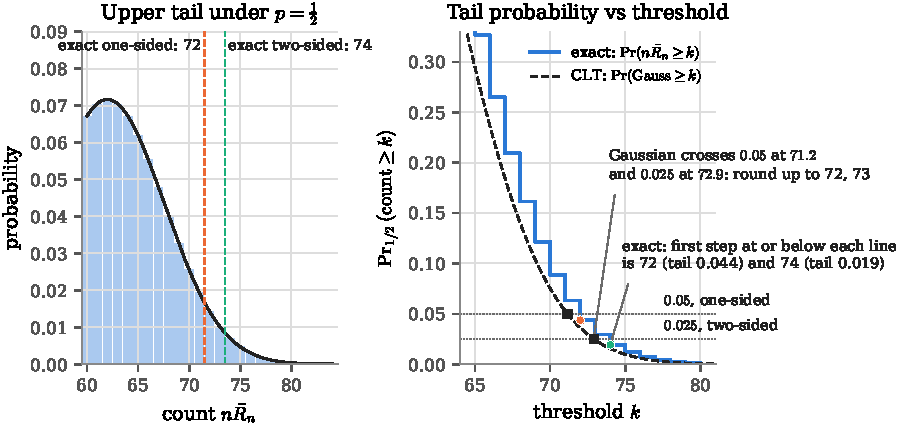
\includegraphics[width=\textwidth]{fig_exact_vs_clt}
\caption{Left: the upper tail of $\mathrm{Bin}(124, \frac12)$ (bars) and the $\Gauss(62, 31)$ density (curve), with the exact thresholds $72$ (orange) and $74$ (aqua) dashed. Right: $\Pr_{1/2}(\text{count} \geq k)$ against $k$, exact (staircase) and Gaussian (dashed), with the levels $0.05$ and $0.025$ dotted.}
\label{fig:exactclt}
\end{figure}

\textbf{Why they differ.}
\Cref{fig:exactclt} shows the two tail probabilities side by side.
On the left is the $\Gauss(62, 31)$ density the CLT puts in place of the $\mathrm{Bin}(124, \frac12)$ bars; on the right is the tail probability $\Pr_{1/2}(\text{count} \geq k)$ as a function of the threshold $k$, a staircase for the exact distribution and a smooth curve for the Gaussian.
The exact threshold is the first step at or below the level line, $72$ for $0.05$ and $74$ for $0.025$; the CLT threshold is where the curve crosses the line, $71.2$ and $72.9$, rounded up to $72$ and $73$.
The Gaussian curve is a good approximation of the staircase, off by about $0.005$ at $k = 73$, but $0.005$ is enough to put the exact tail ($0.029$) above the line $0.025$ and the Gaussian tail ($0.024$) below it, and that is the whole disagreement.
The gap is mostly discreteness, not the CLT's inaccuracy: the Gaussian approximates the probability of the count being $\geq 73$ better if the threshold is placed at $72.5$ (the \textbf{continuity correction} of an introductory course), and with it the two-sided threshold becomes $62 + 0.5 + 10.9 = 73.4$, rounding up to $74$, in agreement with the exact test.
This book does not use the correction. For a proportion, whenever the Gaussian approximation lands close enough to the line that the correction would change the decision, the exact Binomial test is available and settles the question outright. An asymptotic level $5\%$ is not an exact level $5\%$, and at a threshold where the exact tail is near the line the two can round in different directions.
For $80$ right turns, far from either threshold, the decision is the same every way: reject.

\begin{bridge}[the binomial test and the $z$-test for a proportion]
An introductory course presents these as two tests: the `exact binomial test' when $n$ is small, the `$z$-test for a proportion' when $np_0$ and $n(1 - p_0)$ are both at least $10$.
They test the same hypothesis with the same statistic, the count, and differ only in whether the count's distribution under $H_0$ is used as it is or replaced by its Gaussian limit.
The rule of thumb keeps the count's skewness small (the `$np \geq 10$' bridge in \cref{sec:clt}); it does nothing about discreteness, which is why the two-sided thresholds above still differ by one count with $np_0 = 62$.
\end{bridge}

\section{\texorpdfstring{$p$}{p}-values}
\label{sec:tests-pvalue}

A test as defined reports one bit, reject or not, at one level fixed in advance.
That loses information: a $T_n$ of $1.97$ and a $T_n$ of $3.23$ both reject at $5\%$, and the second is much stronger evidence.
It also forces the reader to accept the writer's $\alpha$.
The $p$-value fixes both.

\begin{definition}[$p$-value]
\label{def:pvalue}
Let $(\psi_\alpha)_{\alpha \in (0,1)}$ be a family of tests of $H_0$ indexed by their level, nested so that rejecting at level $\alpha$ implies rejecting at every level above $\alpha$.
The \textbf{(asymptotic) $p$-value} of the family on a given sample is the smallest (asymptotic) level $\alpha$ at which $\psi_\alpha$ rejects $H_0$ on that sample.\footnote{Strictly an infimum: at the boundary level the threshold equals the observed statistic and the strict inequality in $\psi_\alpha$ fails. The boundary case has probability zero, and the golden rule's $\leq$ settles it by convention.}
It is random: it depends on the sample.
\end{definition}

\begin{inwords}
\textbf{In words.} Run the test at every level at once. At large $\alpha$ it rejects easily, at small $\alpha$ it is hard to satisfy; the $p$-value is the level where it switches. Equivalently, for the standardized-mean tests of this chapter, it is the probability under $H_0$ of a test statistic at least as extreme as the one observed: the tail area beyond the observed value.
\par\smallskip
\textbf{For the kiss data.} $T_n = 3.23$. Two-sided, the $p$-value is $\Pr(\abs{Z} > 3.23) = 2(1 - \Phi(3.23)) = 0.0012$; one-sided, $\Pr(Z > 3.23) = 0.0006$. The exact Binomial tails give $0.0016$ and $0.0008$. Under $p = \frac12$, $80$ or more right turns out of $124$ is a one-in-a-thousand event.
\end{inwords}

\begin{figure}[htbp]
\centering
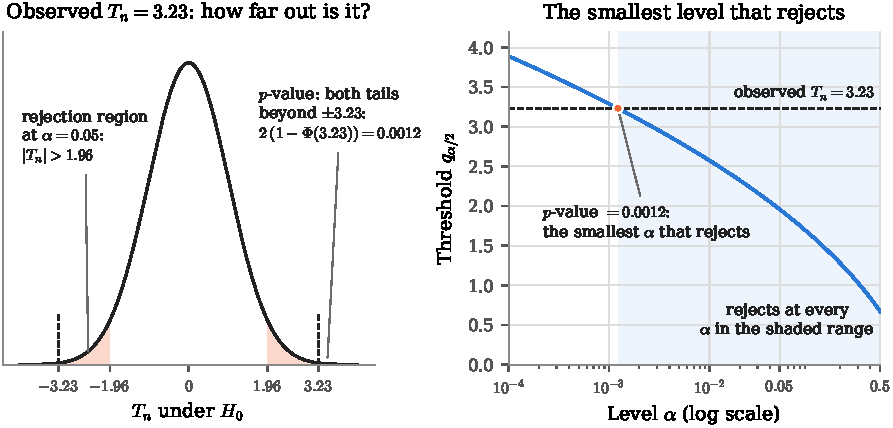
\includegraphics[width=\textwidth]{fig_pvalue}
\caption{The $p$-value for $T_n = 3.23$. Left: the density of $T_n$ under $H_0$, the rejection region at $5\%$ (light orange), the area beyond $\pm 3.23$ (dark orange), the observed value (dashed). Right: the threshold $q_{\alpha/2}$ against the level $\alpha$, with the observed value dashed.}
\label{fig:pvalue}
\end{figure}

\Cref{fig:pvalue} shows the $p$-value two ways.
On the left, the density of $T_n$ under $H_0$ is the standard Gaussian by the CLT, the $5\%$ rejection region is $\abs{T_n} > 1.96$, and the $p$-value is the area beyond $\pm 3.23$, too small to see at this scale: the probability under $H_0$ of something at least this extreme, $0.0012$.
On the right, the threshold $q_{\alpha/2}$ is drawn as a function of the level, with the observed value as a horizontal line; the test rejects at every level whose threshold lies below the line, and the smallest such level, where the curve crosses, is the $p$-value.
The two readings are the same number because of how the thresholds are built.
For the two-sided test, $\psi_\alpha$ rejects when $\abs{T_n} > q_{\alpha/2}$, and $q_{\alpha/2}$ decreases as $\alpha$ grows, so the levels at which the test rejects are exactly those with $q_{\alpha/2} < \abs{t}$ for the observed $t$, that is, those with $\alpha/2 > \Pr(Z > \abs{t})$, that is, $\alpha > \Pr(\abs{Z} > \abs{t})$.
The smallest such $\alpha$ is $\Pr(\abs{Z} > \abs{t})$, the tail area.
For a one-sided test with $H_1: \mu > \mu_0$ the same argument gives $\Pr(Z > t)$.
Since $\Pr(\abs{Z} > \abs{t}) = 2\Pr(Z > \abs{t})$, a two-sided $p$-value is twice the one-sided one when the data lean the alternative's way; when they lean the other way the one-sided $p$-value is above $\frac12$ and the one-sided test cannot reject. That is the one-sided test's advantage of \cref{sec:tests-clt} seen from the other end: it spends its whole $\alpha$ on one side and is blind to the other.

\textbf{The golden rule.}
The consequence of the definition is the rule worth memorizing:
\[
p\text{-value} \leq \alpha \quad \Longleftrightarrow \quad H_0 \text{ is rejected by } \psi_\alpha \text{ at (asymptotic) level } \alpha.
\]
So one number replaces the whole family of tests.
A reader who wants level $5\%$ compares the $p$-value with $0.05$; one who wants $1\%$ compares with $0.01$; and the smaller the $p$-value, the more levels reject, the more confidently $H_0$ is rejected.

\begin{bridge}[$p < 0.05$]
`Reject if $p < 0.05$' was the rule of an introductory course, and the golden rule is its justification: the $p$-value is the smallest level that rejects, so a $p$-value below $0.05$ means the level-$5\%$ test rejects, no more and no less.
Two habits from that course transfer intact. The $p$-value is computed from the null distribution of the statistic, which is why it needed $\mu_0$ (or $p_0$) and not any guess at the alternative. And a one-sided $p$-value is half the two-sided one for a symmetric statistic when the data lean the alternative's way, so the choice of sides made in \cref{sec:tests-hypotheses} before seeing the data is the choice that fixes the $p$-value.
\end{bridge}

\begin{pitfall}[what a $p$-value is not]
A $p$-value of $0.0012$ is the probability, computed as if $H_0$ were true, of data at least as extreme as these.
It is not the probability that $H_0$ is true; in this part of the book $H_0$ is true or false and has no probability (\cref{ch:bayes-intro} is where hypotheses get probabilities, and the number it produces is a different one).
It is not the probability that the result `was due to chance'.
And it is not a measure of the size of the effect: with $n$ large enough, a true $p$ of $0.51$ produces a tiny $p$-value (at $n = 100{,}000$, $T_n = 2\sqrt{n} \times 0.01 = 6.3$), since by \cref{prop:clt-test} the test detects any fixed departure eventually.
The $p$-value answers one question, how surprising the data would be under $H_0$, and the confidence interval of \cref{ch:confidence-intervals} answers the other, how big the departure is.
Report both.
\end{pitfall}

\begin{intuition}[the $p$-value is a statistic, and under $H_0$ it is uniform]
The $p$-value is a function of the sample, so it is a random variable, and it has a distribution under each $\theta$.
Under a simple $H_0$, for a test statistic with a continuous distribution, that distribution is uniform on $[0, 1]$: a $p$-value below $0.05$ happens $5\%$ of the time, below $0.01$ $1\%$ of the time, which is just the level restated (\cref{ex:tests-uniform} proves it).
Under $H_1$ the distribution piles up near $0$, and the more so the larger $n$.
So a small $p$-value is not proof; it is an event that is rare under $H_0$ and common under $H_1$.
\end{intuition}

\section{Tests and confidence intervals are one construction}
\label{sec:tests-duality}

\Cref{ex:ci-onesided} in \cref{ch:confidence-intervals} found that `$\frac12$ is below the conservative lower confidence bound' is the same event as `$n\bar{R}_n \geq 72$', the one-sided test's rejection.
That was not a coincidence of the kiss data.

\begin{proposition}[Duality of tests and confidence intervals]
\label{prop:duality}
Let $\Theta \subseteq \real$.
\begin{enumerate}[nosep]
\item Suppose that for every $\theta_0 \in \Theta$ there is a test $\psi(\theta_0)$ of $H_0: \theta = \theta_0$ with level $\alpha$.
Then the set of values not rejected,
\[
\mathcal{I} = \{ \theta_0 \in \Theta : \psi(\theta_0) = 0 \},
\]
is a confidence set of level $1 - \alpha$ for $\theta$.
\item Conversely, if $\mathcal{I}$ is a confidence interval of level $1 - \alpha$ for $\theta$, then for every $\theta_0$ the test $\psi(\theta_0) = \ind(\theta_0 \notin \mathcal{I})$ has level $\alpha$ for $H_0: \theta = \theta_0$.
\end{enumerate}
The same holds with `asymptotic' in front of both levels.
\end{proposition}

\coreproof{Both directions are one line: the event `the true $\theta$ is not in $\mathcal{I}$' is the event `the test of the true $\theta$ rejects', whose probability is the type 1 error.}
\begin{proof}
(1) For any true $\theta$, $\Pr_\theta(\mathcal{I} \not\ni \theta) = \Pr_\theta(\psi(\theta) = 1) = \alpha_{\psi(\theta)}(\theta) \leq \alpha$, since $\psi(\theta)$ has level $\alpha$ for the null $\theta = \theta$, which is true.
So $\Pr_\theta(\mathcal{I} \ni \theta) \geq 1 - \alpha$ for every $\theta$: the coverage condition of \cref{def:ci}, applied to a set rather than an interval.
(2) Under $H_0: \theta = \theta_0$ the truth is $\theta_0$, and $\Pr_{\theta_0}(\psi(\theta_0) = 1) = \Pr_{\theta_0}(\mathcal{I} \not\ni \theta_0) \leq \alpha$ by the coverage guarantee.
The asymptotic version replaces each probability by its limit.
\end{proof}

\begin{figure}[htbp]
\centering
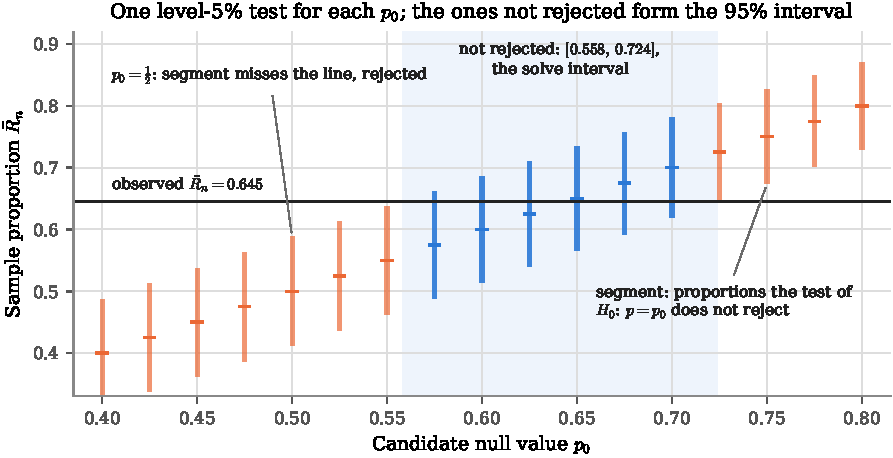
\includegraphics[width=\textwidth]{fig_test_ci_duality}
\caption{The duality for the kiss data. At each candidate $p_0$ (horizontal axis), a vertical segment $p_0 \pm 1.96\sqrt{p_0(1-p_0)/124}$; the horizontal line is the observed $\bar{R}_n = 0.645$. Segments crossing the line are blue, segments missing it are orange, and the shaded strip is $[0.558, 0.724]$.}
\label{fig:duality}
\end{figure}

\Cref{fig:duality} draws part (1) for the kiss data, running the test for every $p_0$ at once.
Each vertical segment is the set of sample proportions the level-$5\%$ test of $H_0: p = p_0$ does not reject; a candidate whose segment crosses the line of the observed $\bar{R}_n = 0.645$ is not rejected, one whose segment misses it is rejected, and $\frac12$ misses.
The shaded strip of candidates not rejected is $[0.558, 0.724]$, the solve interval of \cref{ch:confidence-intervals} exactly.
The test being inverted is
\[
\psi(p_0) = \ind\left\{ \abs{\bar{R}_n - p_0} > q_{\alpha/2}\sqrt{p_0(1 - p_0)/n} \right\},
\]
which measures the distance from $p_0$ in units of the standard error computed \textit{at $p_0$}, the value the null hypothesis asserts. For a proportion, a test built that way, from the standard error under the null rather than from an estimate, is the \textbf{score test}, which \cref{ch:wald-lrt} defines for any model.
The candidates that survive are those with $\abs{\bar{R}_n - p_0} \leq q_{\alpha/2}\sqrt{p_0(1-p_0)/n}$, which is the inequality that \cref{sec:ci-three-solutions} solved to get the solve interval $[0.558, 0.724]$.
So the solve interval is the set of null values the score test does not reject, and the score test of $p = \frac12$ rejects exactly because $\frac12$ is outside the interval. This is why \cref{sec:ci-three-solutions} called the result the Wilson score interval: it is the score test, inverted.
Inverting the test built from the \textit{estimated} standard error $\sqrt{\bar{R}_n(1 - \bar{R}_n)/n}$ instead gives the plug-in interval $[0.561, 0.729]$. That one is \textbf{Wald's test}, which \cref{ch:wald-lrt} treats in general. Score and Wald are the same idea evaluated at two different places, the null value and the estimate, and they are the two tests you will meet most often.
And the one-sided test of \cref{ex:ci-onesided} inverts to a one-sided interval, a lower confidence bound.
Every interval in \cref{ch:confidence-intervals} is a test turned inside out, and every test here is an interval asked about one point.

\begin{bridge}[if the confidence interval excludes the null value, reject]
An introductory course states this as a shortcut: `the $95\%$ confidence interval is $[0.56, 0.73]$, which does not contain $0.5$, so the difference is significant at $5\%$'.
\Cref{prop:duality} is why the shortcut is legitimate, and it also says when it is exact and when it is approximate.
The shortcut reproduces the test's decision exactly when the test and the interval are built from the same standard error, the solve interval for the score test and the plug-in interval for Wald's, and only approximately otherwise.
Using the plug-in interval to decide a score test can disagree with it on a borderline sample, since the two standard errors differ: $\sqrt{\bar{R}_n(1 - \bar{R}_n)/n} = 0.043$ against $\sqrt{\frac12 \cdot \frac12 / n} = 1/(2\sqrt{n}) = 0.045$ here. Far from the border, as with $80$ picks, every version agrees.
\end{bridge}

\section{What comes next}
\label{sec:tests-next}

This chapter built one test, the standardized mean against a Gaussian quantile, and the ideas that describe any test.
The remaining tests in this book are the same object with a different statistic and a different null distribution.
\Cref{ch:t-test} replaces the Gaussian quantile by a Student quantile when $n$ is small and the data are Gaussian, which needs the chi-squared distribution and Cochran's theorem for the sample variance; it also finishes the boarding example as a two-sample test.
\Cref{ch:wald-lrt} gives three general recipes for a test statistic in any parametric model, Wald's test (the standardized maximum likelihood estimator), the likelihood ratio test and the score test, with chi-squared limits in place of Gaussian ones.
\Cref{ch:gof} and \cref{ch:ks} test the model itself rather than a parameter in it, with the same vocabulary: a statistic, a null distribution, a threshold, a $p$-value.
In all of them the level is the cap on the type 1 error, the power is what the test can detect, and the $p$-value is what gets reported.

\section{Summary}
\label{sec:tests-summary}

\begin{itemize}[nosep]
\item Hypotheses: $H_0: \theta \in \Theta_0$ against $H_1: \theta \in \Theta_1$, disjoint. The data are used only to try to reject $H_0$; failing to reject is not accepting. Simple ($\{\theta_0\}$) or composite; one-sided or two-sided, and the side is chosen before the data are seen.
\item A test is $\psi: E^n \to \{0,1\}$, the indicator of its rejection region; in practice $\psi = \ind(T_n > c)$ for a test statistic $T_n$ and a threshold $c$.
\item Type 1 error $\alpha_\psi(\theta) = \Pr_\theta(\psi = 1)$ on $\Theta_0$; type 2 error $\beta_\psi(\theta) = \Pr_\theta(\psi = 0)$ on $\Theta_1$; power $\pi_\psi = \inf_{\Theta_1}(1 - \beta_\psi)$. At fixed $n$ the two errors trade off; only $n$ lowers both.
\item Level $\alpha$: $\alpha_\psi \leq \alpha$ on all of $\Theta_0$, a cap on the worst case; asymptotic level: the same in the limit. For a composite null the worst case is at the boundary, so $H_0: \theta \leq \theta_0$ and $H_0: \theta = \theta_0$ get the same test. For a test the level is $\alpha$; for an interval it is $1 - \alpha$.
\item The standardized-mean test: $T_n = \sqrt{n}(\bar{X}_n - \mu_0)/\sigma$, reject if $\abs{T_n} > q_{\alpha/2}$ (two-sided) or $T_n > q_\alpha$ (one-sided). Asymptotic level $\alpha$ by the CLT, plus Slutsky if $\sigma$ is estimated; consistent (power $\to 1$ at every fixed alternative) by the LLN. Under $H_0$ the parameter is known, so no plug-in is needed.
\item Kiss experiment: $T_n = 3.23$, reject at $5\%$ either way. Exact Binomial thresholds $72$ (one-sided) and $74$ (two-sided); CLT thresholds $72$ and $73$. They differ because the exact tail is a staircase and $0.025$ falls between two of its steps.
\item $p$-value: the smallest level at which the data reject; for these tests, the tail area beyond the observed statistic under $H_0$. Golden rule: $p$-value $\leq \alpha$ if and only if $\psi_\alpha$ rejects. Kiss experiment: $0.0012$ two-sided, $0.0006$ one-sided. Not the probability that $H_0$ is true.
\item Duality: the null values a level-$\alpha$ test does not reject form a level-$(1-\alpha)$ confidence set, and a level-$(1-\alpha)$ interval rejects every null value outside it at level $\alpha$. The solve interval inverts the score test, which uses the standard error at the null value; the plug-in interval inverts Wald's test, which uses the estimated standard error.
\end{itemize}

\section{Exercises}
\label{sec:tests-exercises}

\begin{exercise}
\label{ex:tests-kiss-pvalue}
For $80$ of $124$ couples turning right, formulate the two-sided hypothesis problem, compute the $p$-value by the CLT and exactly, and conclude. Then do the one-sided version.
\end{exercise}
\begin{solution}
$H_0: p = \frac12$ against $H_1: p \neq \frac12$ in the model $(\{0,1\}, (\Bern(p))_{p \in (0,1)})$. $T_n = 2\sqrt{124}(0.6452 - 0.5) = 3.23$. CLT $p$-value: $2(1 - \Phi(3.23)) = 0.0012$. Exact: $\Pr_{1/2}(n\bar{R}_n \geq 80) = 0.0008$, doubled for two sides, $0.0016$. Both are far below $0.05$ (and below $0.01$): reject $H_0$ at any conventional level; the data are not compatible with equal appeal. One-sided, $H_1: p > \frac12$: $p$-values $1 - \Phi(3.23) = 0.0006$ (CLT) and $0.0008$ (exact), half the two-sided ones.
\end{solution}

\begin{exercise}
\label{ex:tests-cookies}
(From OpenIntro Statistics.) Students count the chocolate chips in $32$ cookies and find a mean of $14.77$ with a standard deviation of $4.37$. The packaging claims at least $20$ chips per cookie. One student says the claim is unreasonable; another says the difference might be chance. Formulate the hypotheses, compute a $p$-value and decide, saying what approximation you used.
\end{exercise}
\begin{solution}
Let $\mu$ be the mean number of chips. The claim is the null, $H_0: \mu \geq 20$, and the student's doubt is the alternative, $H_1: \mu < 20$: a one-sided test with the threshold computed at the boundary $\mu_0 = 20$. With $\sigma$ replaced by the sample standard deviation, $T_n = \sqrt{32}\,(14.77 - 20)/4.37 = -6.77$. By the CLT and Slutsky the $p$-value is approximately $\Phi(-6.77) \approx 6 \times 10^{-12}$: reject at every conventional level; the difference is not chance. The approximation is the Gaussian limit at $n = 32$ with an estimated $\sigma$; \cref{ch:t-test} replaces it by Student's $t$ with $31$ degrees of freedom, for which $-6.77$ is just as decisive.
\end{solution}

\begin{exercise}
\label{ex:tests-cancer}
A machine learning procedure claims to reduce the rate of surgery on benign tumors below the state of the art, $95\%$, while keeping the true positive rate. On $297$ benign tumors it recommended surgery for $206$. Let $p$ be the proportion of benign tumors on which it prescribes surgery. Formulate the hypotheses, compute the $p$-value and conclude.
\end{exercise}
\begin{solution}
The claim needs evidence, so it is the alternative: $H_0: p \geq 0.95$ against $H_1: p < 0.95$, one-sided, threshold at the boundary $p_0 = 0.95$. $\hat{p} = 206/297 = 0.6936$ and $T_n = \sqrt{297}\,(0.6936 - 0.95)/\sqrt{0.95 \times 0.05} = -20.3$. The $p$-value $\Phi(-20.3)$ is zero to every decimal place anyone prints: reject $H_0$; the procedure's false positive rate is below $95\%$. (Whether it is below by enough to matter is the confidence interval's question: $0.694 \pm 1.96\sqrt{0.694 \times 0.306/297} = [0.64, 0.75]$.)
\end{solution}

\begin{exercise}
\label{ex:tests-coin}
For the fair coin ($13$ heads in $30$ tosses), compute the two-sided $p$-value by the CLT and exactly, and comment on the gap.
\end{exercise}
\begin{solution}
$T_n = -0.73$, CLT $p$-value $2\Phi(-0.73) = 0.47$. Exactly, $\Pr_{1/2}(\mathrm{Bin}(30, \frac12) \leq 13) = 0.292$, doubled $0.58$. Neither is close to rejecting. The gap between $0.47$ and $0.58$ is the discreteness of \cref{fig:exactclt} at $n = 30$: the Gaussian tail beyond $13$ undercounts the mass of the bar at $13$ itself, which the continuity correction (evaluating at $13.5$) largely repairs: $2\Phi(\sqrt{30}(13.5/30 - 0.5)/0.5) = 2\Phi(-0.55) = 0.58$.
\end{solution}

\begin{exercise}
\label{ex:tests-interval-null}
For $\Xton \iid \Pois(\lambda)$, build a test of asymptotic level $5\%$ for $H_0: \abs{\lambda - 2} \leq 1$ against $H_1: \abs{\lambda - 2} > 1$.
\end{exercise}
\begin{solution}
$\Theta_0 = [1, 3]$. Reject when $\hat{\lambda}$ is far outside it on either side, with a margin that shrinks like $1/\sqrt{n}$ and uses the standard deviation $\sqrt{\lambda}$ at its own endpoint: $\psi = \ind(\hat{\lambda} > 3 + s\sqrt{3/n}) + \ind(\hat{\lambda} < 1 - s\sqrt{1/n})$ for a number $s$ to be chosen (the two events are disjoint, since $\hat{\lambda}$ cannot be both above $3$ and below $1$). The type 1 error at $\lambda \in [1, 3]$ is largest at the endpoints: at $\lambda = 3$ the first indicator is the event $\sqrt{n}(\hat{\lambda} - 3)/\sqrt{3} > s$, whose probability tends to $\Pr(Z > s)$ by the CLT, and the second indicator's probability tends to $0$ by the LLN; at $\lambda = 1$ the reverse, with limit $\Pr(Z < -s)$. At any interior $\lambda$ both probabilities tend to $0$. Choosing $s = 1.645$ makes each endpoint's limiting type 1 error $0.05$, so the test has asymptotic level $5\%$ (not $2.5\%$ per side: at any one $\lambda$ only one side can fire in the limit). Each side uses the standard deviation $\sqrt{\lambda}$ at its own endpoint, which is the `parameter known under the null' idea applied endpoint by endpoint.
\end{solution}

\begin{exercise}
\label{ex:tests-uniform}
Let $T$ be a test statistic with a continuous, strictly increasing CDF $F_0$ under $H_0$, and let the test reject for large $T$, so the $p$-value is $P = 1 - F_0(T)$. Show that under $H_0$, $P$ is uniform on $[0, 1]$, and deduce that $\Pr_{H_0}(P \leq \alpha) = \alpha$ for every $\alpha$: the golden rule gives exact level $\alpha$.
\end{exercise}
\begin{solution}
For $u \in (0, 1)$, $\Pr_{H_0}(P \leq u) = \Pr_{H_0}(1 - F_0(T) \leq u) = \Pr_{H_0}(F_0(T) \geq 1 - u) = \Pr_{H_0}(T \geq F_0^{-1}(1 - u)) = 1 - F_0(F_0^{-1}(1 - u)) = u$, using that $F_0$ is continuous and strictly increasing so that $F_0^{-1}$ exists and $\Pr(T = t) = 0$ \toolkit{sec:math-density}. A CDF equal to $u$ on $(0,1)$ is the uniform CDF. Then $\Pr_{H_0}(P \leq \alpha) = \alpha$, which is the golden rule's `reject when $P \leq \alpha$' having type 1 error exactly $\alpha$. For a discrete $T$ the equality becomes $\leq \alpha$, the staircase of \cref{sec:tests-kiss}.
\end{solution}

\begin{exercise}
\label{ex:tests-solve-inversion}
Show that the set of $p_0 \in (0,1)$ not rejected by the test $\psi(p_0) = \ind(\abs{\bar{R}_n - p_0} > q_{\alpha/2}\sqrt{p_0(1 - p_0)/n})$ is exactly the solve interval of \cref{sec:ci-three-solutions}, and that inverting the test with the plug-in standard error gives the plug-in interval.
\end{exercise}
\begin{solution}
Not rejecting $p_0$ means $\abs{\bar{R}_n - p_0} \leq q_{\alpha/2}\sqrt{p_0(1-p_0)/n}$, that is, $(\bar{R}_n - p_0)^2 \leq q_{\alpha/2}^2\, p_0(1 - p_0)/n$, the quadratic inequality in $p_0$ whose solution set is the solve interval (\cref{eq:wilson}). With $\sqrt{\bar{R}_n(1 - \bar{R}_n)/n}$ in place of $\sqrt{p_0(1-p_0)/n}$ the inequality is $\abs{\bar{R}_n - p_0} \leq q_{\alpha/2}\sqrt{\bar{R}_n(1 - \bar{R}_n)/n}$, whose solution set is $\bar{R}_n \pm q_{\alpha/2}\sqrt{\bar{R}_n(1-\bar{R}_n)/n}$, the plug-in interval. The conservative interval inverts the test that uses the worst-case standard error $1/(2\sqrt{n})$ for every $p_0$.
\end{solution}


\partintro{Part III judged estimators; this part produces them. The distances between distributions of \cref{ch:distances} say what `close to the truth' means; maximum likelihood (\cref{ch:likelihood,ch:mle-properties}) is the main method, with its consistency and asymptotic normality through the Fisher information; the method of moments and M-estimation (\cref{ch:mom-mestimation}) are the two generalizations.}
\part{Methods of Estimation}
\chapter[Distances Between Distributions]{Distances Between Distributions: Total Variation and Kullback--Leibler}
\label{ch:distances}

\begin{chaptergoals}
\begin{itemize}[nosep]
\item Why `the estimate is close to the truth' should be measured between distributions and not between parameters, and an example where a parameter difference of $0.01$ means almost nothing in one place and a great deal in another.
\item Total variation: the largest disagreement between two distributions over all events, equal to the area between their densities. What it says about tests: the best possible test between two distributions has $\alpha + \beta = 1 - \TV$.
\item Why total variation, for all its good properties, can't be estimated by an average of the data.
\item The Kullback--Leibler divergence: the average evidence one observation supplies against the wrong distribution. Its properties, its asymmetry, why it adds up over independent observations, and why near the truth it is a parabola.
\item Estimating the KL divergence by the Law of Large Numbers, and the discovery that minimizing the estimate is maximizing the likelihood.
\item What an estimator estimates when the model is wrong: the member of the family closest to the truth in KL. For the Gaussian family that is the member with the right mean and variance.
\end{itemize}
Part III judged estimators that were handed to you. This chapter is the first step toward producing them: it says what `close' means, and the answer leads straight to maximum likelihood in \cref{ch:likelihood}.
\end{chaptergoals}

\section{What `close to the truth' should mean}
\label{sec:dist-close}

Go back to the setup of \cref{ch:models}.
You have a statistical model $(E, (\Pr_\theta)_{\theta \in \Theta})$, data $\Xton \iid \Pr_{\theta^*}$ from a true parameter $\theta^*$ that you don't know, and an estimator $\hat{\theta}_n$.
What would it mean for $\hat{\theta}_n$ to be a good estimator?

The answer of \cref{ch:estimators} was that $\hat{\theta}_n$ should be close to $\theta^*$ as numbers: small bias, small variance, small quadratic risk $\E[(\hat{\theta}_n - \theta^*)^2]$.
That is a fine answer when the parameter is the thing you care about, like the share of couples who turn right.
But a parameter is a label for a distribution.
What you actually use a fitted model for is its distribution: the probability it assigns to an interval, a tail, a range of outcomes.
So the question you'd really like answered is whether the fitted distribution $\Pr_{\hat{\theta}_n}$ is close to the true one $\Pr_{\theta^*}$, in the sense that for every event $A$,
\[
\Pr_{\hat{\theta}_n}(A) \approx \Pr_{\theta^*}(A).
\]
If that holds, every probability you compute from the fitted model is about right, and that is the whole point of fitting it.

\begin{intuition}[a parameter difference has no fixed meaning]
Is a difference of $0.01$ between two parameters small?
It depends on where in the parameter space it happens.
Two Gaussians with standard deviation $1$ whose means differ by $0.01$ are, for every practical purpose, the same distribution: no event has probabilities under the two that differ by more than $0.004$.
Two Gaussians with mean $0$ whose standard deviations are $0.01$ and $0.02$ also have parameters $0.01$ apart, and they are obviously different distributions: one is twice as wide as the other, and there is an event whose probability is $0.32$ higher under one than under the other.
\Cref{fig:paramvsdist} draws both.
\end{intuition}

\begin{figure}[htbp]
\centering
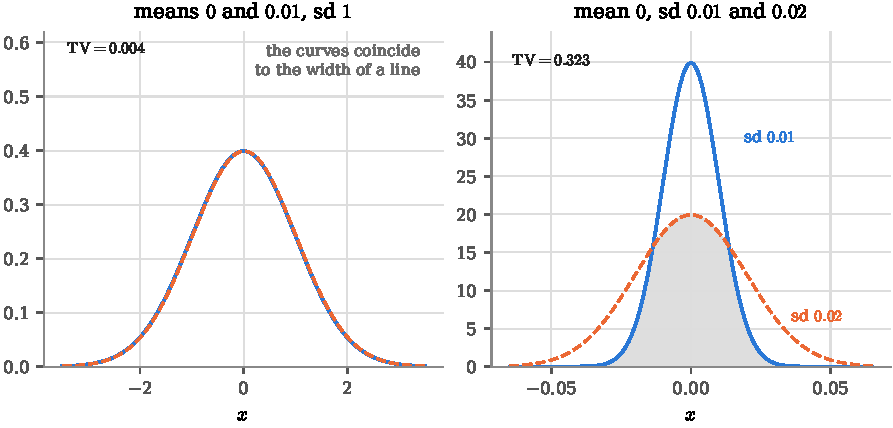
\includegraphics[width=\textwidth]{fig_param_vs_dist}
\caption{Two pairs of Gaussians whose parameters differ by $0.01$. Left: means $0$ and $0.01$, standard deviation $1$; the curves coincide to the width of a line and the total variation distance is $0.004$. Right: mean $0$, standard deviations $0.01$ and $0.02$; the curves share only the gray area, $0.677$, so the total variation distance is $0.323$.}
\label{fig:paramvsdist}
\end{figure}

There is a second reason to measure closeness between distributions, and it matters as much as the first.
\Cref{sec:models-wellspecified} asked whether the model is well-specified, whether the true distribution is in the family at all.
If it isn't, there is no $\theta^*$, and `the distance from $\hat{\theta}_n$ to $\theta^*$' has no meaning.
A distance between distributions still has one: you can ask which member of the family is closest to the truth, even when none of them is the truth.
\Cref{sec:dist-projection} answers that question.

The chapter builds two such measures.
The first, total variation, is the natural one, and it is a true distance.
The second, the Kullback--Leibler divergence, is not a true distance, and it is the one statistics uses, for a reason that takes \cref{sec:dist-tv-estimate} to explain.

\section{Total variation}
\label{sec:dist-tv}

The requirement `$\Pr(A) \approx \Qr(A)$ for every event $A$' already contains a definition.
Look at all the events, find the one on which the two distributions disagree most, and call that disagreement the distance.

\begin{definition}[Total variation distance]
\label{def:tv}
Let $\Pr$ and $\Qr$ be two probability distributions on the same sample space $E$.
The \textbf{total variation distance} between them is
\[
\TV(\Pr, \Qr) = \max_{A \subset E} \abs{\Pr(A) - \Qr(A)},
\]
the largest difference between the probabilities they assign to one event.
\end{definition}

\begin{inwords}
\textbf{In words.} Run through every question you could ask about one draw (is it positive? is it between $2$ and $3$? is it even?) and record how differently the two distributions answer. The total variation distance is the worst case. If it is $0.01$, no question you could ever ask gets answers more than one percentage point apart. That is exactly the guarantee you want from a fitted model: every probability it reports is within $\TV$ of the true one.
\par\smallskip
\textbf{For the kiss data.} One couple either turns right or doesn't, so there are four events: nothing, `right', `left' and everything. Compare $\Bern(0.645)$, the fitted distribution, with $\Bern(\frac12)$, `no preference'. The empty event and the whole space get probabilities $0$ and $1$ from both. `Right' gets $0.645$ and $0.5$; `left' gets $0.355$ and $0.5$. The largest difference is $0.145$, so $\TV = 0.145$. As a natural frequency: of $1{,}000$ couples, the fitted model predicts $645$ right turns and `no preference' predicts $500$; the two descriptions disagree about $145$ couples in a thousand.
\end{inwords}

For a sample space with four events the maximum is easy.
For a sample space like $\real$ there are uncountably many events, and searching over them is not a calculation anyone wants to do.
The next result turns the maximum into a sum or an integral.

\begin{proposition}[Total variation as an area]
\label{prop:tv-area}
If $\Pr$ and $\Qr$ have PMFs $p$ and $q$ on a discrete $E$,
\[
\TV(\Pr, \Qr) = \frac12 \sum_{x \in E} \abs{p(x) - q(x)};
\]
if they have densities $p$ and $q$,
\[
\TV(\Pr, \Qr) = \frac12 \int_E \abs{p(x) - q(x)} \, \mathrm{d}x.
\]
The maximum in \cref{def:tv} is attained at the event $A^\star = \{x : p(x) > q(x)\}$, where $\Pr$ puts more mass than $\Qr$.
\end{proposition}

\coreproof{The event that favors $\Pr$ most collects every point where $p$ beats $q$ and no other point. Its advantage is the area of the region where $p$ is above $q$; the region where $q$ is above $p$ has the same area, since both densities have total mass $1$. Half the total area between the curves is therefore the area of either piece.}
\begin{proof}
The discrete case; the continuous one replaces sums by integrals.
Split $E$ into $A^\star = \{p > q\}$ and its complement $\{p \leq q\}$.
For any event $A$,
\[
\Pr(A) - \Qr(A) = \sum_{x \in A} \big(p(x) - q(x)\big) \leq \sum_{x \in A \cap A^\star} \big(p(x) - q(x)\big) \leq \sum_{x \in A^\star} \big(p(x) - q(x)\big) = \Pr(A^\star) - \Qr(A^\star).
\]
The first inequality drops the points of $A$ where $p - q \leq 0$, which can only increase the sum; the second adds the points of $A^\star$ that $A$ missed, where $p - q > 0$, which can only increase it again.
The same argument with $\Pr$ and $\Qr$ exchanged gives $\Qr(A) - \Pr(A) \leq \Qr(A^{\star c}) - \Pr(A^{\star c})$.
Both $p$ and $q$ sum to $1$, so
\[
\sum_{x \in A^\star} \big(p(x) - q(x)\big) + \sum_{x \notin A^\star} \big(p(x) - q(x)\big) = 1 - 1 = 0,
\]
which says that $\Pr(A^\star) - \Qr(A^\star) = \Qr(A^{\star c}) - \Pr(A^{\star c})$: the area where $p$ is above $q$ equals the area where $q$ is above $p$.
Call this common value $D$.
Every event has $\abs{\Pr(A) - \Qr(A)} \leq D$, and $A^\star$ attains it, so $\TV(\Pr, \Qr) = D$.
Finally $\sum_x \abs{p(x) - q(x)}$ is the sum of the two pieces, $D + D = 2D$, and so $D = \frac12 \sum_x \abs{p(x) - q(x)}$.
\end{proof}

\Cref{fig:tvarea} is the proposition as a picture.
Lay the two densities on top of each other.
Where they overlap, the gray region, they agree.
Where they don't, the area splits into two pieces of equal size, one where $p$ is above and one where $q$ is above, and the total variation distance is the area of either piece.
Equivalently, $1 - \TV$ is the area of the overlap, the probability mass the two distributions share.

\begin{figure}[htbp]
\centering
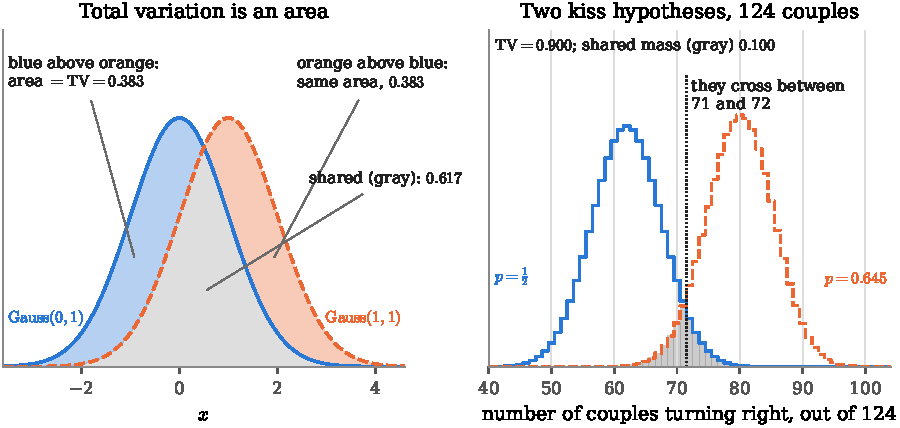
\includegraphics[width=\textwidth]{fig_tv_area}
\caption{Total variation as an area. Left: $\Gauss(0,1)$ and $\Gauss(1,1)$. The blue region, where the first density is above the second, and the orange region, where the second is above the first, have the same area, $0.383$, which is the total variation distance; the gray overlap has area $1 - 0.383 = 0.617$. Right: the distributions of the number of right turns among $124$ couples when $p = \frac12$ and when $p = 0.645$. They share only $0.100$ of their mass (gray), so $\TV = 0.900$, and the two PMFs cross between $71$ and $72$.}
\label{fig:tvarea}
\end{figure}

\begin{worked}[four total variation distances]
\begin{itemize}
\item \textbf{Two Bernoullis.} For $\Bern(p)$ and $\Bern(q)$ the PMFs differ by $\abs{p - q}$ at $1$ and by $\abs{(1-p) - (1-q)} = \abs{p - q}$ at $0$, so
\[
\TV(\Bern(p), \Bern(q)) = \tfrac12\big(\abs{p - q} + \abs{p - q}\big) = \abs{p - q}.
\]
For the kiss data, $\abs{0.645 - 0.5} = 0.145$, as the in-words box found by listing events. For $\Bern(\frac12)$ against $\Bern(\frac1{10})$, $0.4$.
\item \textbf{Two Gaussians with the same variance.} The densities of $\Gauss(0, 1)$ and $\Gauss(\mu, 1)$, $\mu > 0$, cross at the midpoint $\mu/2$, and $A^\star = \{x < \mu/2\}$ is where the first is above. So $\TV = \Pr(Z < \mu/2) - \Pr(Z + \mu < \mu/2) = \Phi(\mu/2) - \Phi(-\mu/2) = 2\Phi(\mu/2) - 1$ for $Z \sim \Gauss(0,1)$. With $\mu = 1$ this is $0.383$, the left of \cref{fig:tvarea}; with $\mu = 0.01$ it is $0.004$, the left of \cref{fig:paramvsdist}.
\item \textbf{An exponential and a uniform.} $\Expo(1)$ has density $e^{-x}$ on $[0, \infty)$, and $\Unif([0,1])$ has density $1$ on $[0,1]$. The two need a common sample space, and $[0, \infty)$ contains both. On $[0,1]$, $1 \geq e^{-x}$; beyond $1$, only the exponential has mass. So
\[
\TV = \frac12 \left( \int_0^1 (1 - e^{-x}) \, \mathrm{d}x + \int_1^\infty e^{-x} \, \mathrm{d}x \right) = \frac12 \left( (1 - 1 + e^{-1}) + e^{-1} \right) = e^{-1} = 0.368.
\]
\item \textbf{Number of right turns.} $\Bin(124, \frac12)$ against $\Bin(124, 0.645)$: half the sum of $125$ absolute differences, computed by machine, is $0.900$. One couple's distributions are $0.145$ apart; $124$ couples' are $0.900$ apart. \Cref{sec:dist-tv-tests} says what that growth means.
\end{itemize}
\end{worked}

\begin{proposition}[Total variation is a distance]
\label{prop:tv-metric}
For distributions $\Pr$, $\Qr$, $\mathbb{V}$ on the same $E$:
\begin{enumerate}[nosep]
\item \textbf{symmetry:} $\TV(\Pr, \Qr) = \TV(\Qr, \Pr)$;
\item \textbf{bounds:} $0 \leq \TV(\Pr, \Qr) \leq 1$, with $\TV = 1$ exactly when there is an event that has probability $1$ under one and $0$ under the other;
\item \textbf{definiteness:} $\TV(\Pr, \Qr) = 0$ only if $\Pr = \Qr$;
\item \textbf{triangle inequality:} $\TV(\Pr, \Qr) \leq \TV(\Pr, \mathbb{V}) + \TV(\mathbb{V}, \Qr)$.
\end{enumerate}
\end{proposition}

\optionalproof{Each property holds for every single event, and taking the maximum over events keeps it.}
\begin{proof}
(1) $\abs{\Pr(A) - \Qr(A)} = \abs{\Qr(A) - \Pr(A)}$.
(2) Every $\abs{\Pr(A) - \Qr(A)}$ is a difference of two numbers in $[0,1]$, so it lies in $[0,1]$. It equals $1$ only if one probability is $1$ and the other is $0$.
(3) If the maximum over events is $0$, every event has the same probability under both, and that is what $\Pr = \Qr$ means.
(4) For each event, $\abs{\Pr(A) - \Qr(A)} \leq \abs{\Pr(A) - \mathbb{V}(A)} + \abs{\mathbb{V}(A) - \Qr(A)}$ by the triangle inequality for numbers \toolkit{sec:math-inequalities}, and each term on the right is at most the corresponding total variation. Take the maximum over $A$ on the left.
\end{proof}

A total variation of $1$ means the two distributions live on separate parts of the sample space: one draw tells you, with certainty, which one it came from.
A total variation of $0$ means they are the same.
Everything else is in between, and \cref{sec:dist-tv-tests} makes `in between' precise.

\begin{bridge}[effect sizes and overlap]
An introductory course measured how far apart two groups are with Cohen's $d$, the difference in means in units of the standard deviation, and called $0.2$ small, $0.5$ medium and $0.8$ large.
For two Gaussians with a common standard deviation, $d$ is a parameter distance, and the second item of the worked example converts it to a distance between distributions: $\TV = 2\Phi(d/2) - 1$.
\Cref{fig:tvcohen} draws the three conventional sizes.
A `large' effect still leaves the two distributions sharing $69\%$ of their mass, and a `small' one leaves them sharing $92\%$.
The shared area $1 - \TV$ is what some texts call the overlapping coefficient, and $\TV$ is the share of each group that has no counterpart in the other.
With equal numbers in the two groups, the best rule for guessing which group one person came from is right with probability $(1 + \TV)/2$, which at $d = 0.8$ is $0.66$.
\end{bridge}

\begin{figure}[htbp]
\centering
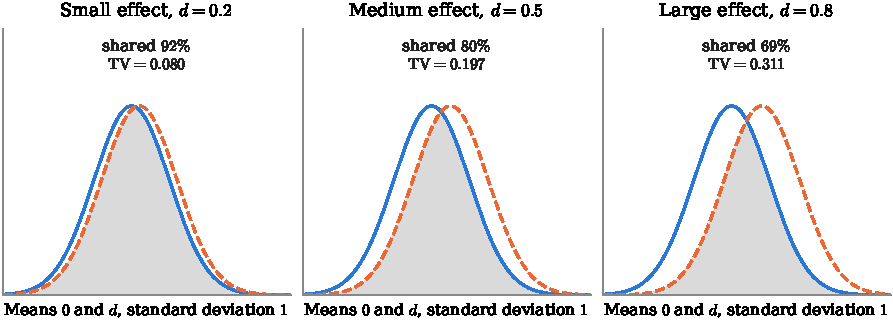
\includegraphics[width=\textwidth]{fig_tv_cohen}
\caption{Cohen's three conventional effect sizes as total variation distances between $\Gauss(0,1)$ (blue, solid) and $\Gauss(d,1)$ (orange, dashed). The shared mass (gray) is $92\%$, $80\%$ and $69\%$; the total variation distances are $0.080$, $0.197$ and $0.311$.}
\label{fig:tvcohen}
\end{figure}

\begin{pitfall}[total variation does not know which outcomes are near each other]
Let $X \sim \Bern(\frac12)$ and $a = 0.001$.
The random variable $X + a$ is $X$ shifted by a thousandth, and any reasonable notion of `close' should call the two distributions close.
Total variation calls them as far apart as two distributions can be: $X$ lives on $\{0, 1\}$, $X + a$ on $\{0.001, 1.001\}$, the event $\{0, 1\}$ has probability $1$ under the first and $0$ under the second, and $\TV = 1$.
Total variation compares probabilities point by point; it has no idea that $0$ and $0.001$ are neighbors.
The same thing happens with the CLT.
\recall{The Central Limit Theorem (\cref{thm:clt}): for iid data with mean $\mu$ and variance $\sigma^2$, $\sqrt{n}(\bar{X}_n - \mu)/\sigma \convd \Gauss(0,1)$.}
For $\Xton \iid \Bern(\frac12)$, $2\sqrt{n}(\bar{X}_n - \frac12) \convd \Gauss(0,1)$, but $2\sqrt{n}(\bar{X}_n - \frac12)$ takes only the $n + 1$ values $2\sqrt{n}(k/n - \frac12)$, a set that has probability $1$ under its own distribution and probability $0$ under any continuous one.
So the total variation distance between the standardized mean and its Gaussian limit is $1$ for every $n$.
Convergence in distribution (\cref{def:convd}) is not convergence in total variation, and it can't be: a discrete distribution is never close to a continuous one in total variation, however finely its mass is spread.
\end{pitfall}

\section{What total variation says about tests}
\label{sec:dist-tv-tests}

Total variation has an operational meaning that makes `in between' concrete: it measures how well data from one distribution can be told apart from data from the other.

Suppose you have to decide, from one draw $X$, whether it came from $\Pr$ or from $\Qr$.
This is the test of \cref{ch:tests-foundations} with $H_0: X \sim \Pr$ and $H_1: X \sim \Qr$, both simple.
A test is an event $R$, the rejection region, and its two errors are $\alpha = \Pr(R)$, rejecting when $\Pr$ is true, and $\beta = \Qr(R^c)$, not rejecting when $\Qr$ is true.
How small can the two errors be together?

\begin{proposition}[The best test and total variation]
\label{prop:tv-best-test}
For every test $R$ of $\Pr$ against $\Qr$,
\[
\alpha + \beta = \Pr(R) + \Qr(R^c) \geq 1 - \TV(\Pr, \Qr),
\]
with equality for the test that rejects where $\Qr$'s density is larger, $R = \{x : q(x) > p(x)\}$.
\end{proposition}

\coreproof{Rewrite $\alpha + \beta$ as $1$ minus the advantage $\Qr(R) - \Pr(R)$ the rejection region gives the alternative. That advantage can never exceed $\TV$, and the region where $q$ beats $p$ achieves it.}
\begin{proof}
$\Qr(R^c) = 1 - \Qr(R)$, so $\alpha + \beta = 1 - \big(\Qr(R) - \Pr(R)\big)$.
By \cref{def:tv}, $\Qr(R) - \Pr(R) \leq \TV(\Pr, \Qr)$ for every event $R$, which gives the inequality.
By \cref{prop:tv-area} with the roles of $\Pr$ and $\Qr$ exchanged, the event $\{q > p\}$ attains the maximum, which gives the equality.
\end{proof}

\begin{intuition}[total variation is distinguishability]
Read \cref{prop:tv-best-test} at its two ends.
If $\TV = 0$, the two distributions are the same, and every test has $\alpha + \beta = 1$ exactly, no better than a test that ignores the data.
If $\TV = 1$, the two live on separate parts of $E$, and the test `reject if $X$ lands in $\Qr$'s part' makes no errors at all.
In between, $1 - \TV$ is the irreducible error: the total of the two error rates that no test, however clever, can get below.
In \cref{fig:tvarea} it is the gray overlap.
A draw that lands in the overlap could have come from either distribution, and that is where every test makes its mistakes.
\end{intuition}

\begin{worked}[how distinguishable is `no preference' from the kiss data?]
For one couple, $\TV(\Bern(\frac12), \Bern(0.645)) = 0.145$, so the best test based on a single couple has $\alpha + \beta \geq 0.855$: almost no better than a coin flip.

For $124$ couples, the relevant distributions are those of the count of right turns, $\Bin(124, \frac12)$ and $\Bin(124, 0.645)$; the order in which the couples turned carries no information about $p$, so the count is all that matters.
Their total variation is $0.900$, so the best test has $\alpha + \beta = 0.100$.
The right of \cref{fig:tvarea} shows where the best test rejects: where the $0.645$ PMF is above the $\frac12$ PMF, which is from $72$ right turns up.
Its two errors are
\[
\alpha = \Pr_{1/2}(\text{count} \geq 72) = 0.0438, \qquad \beta = \Pr_{0.645}(\text{count} \leq 71) = 0.0567,
\]
and they add up to $0.100$.
In natural frequencies: of $1{,}000$ studies of $124$ couples in a world with no preference, the best test cries `preference' in about $44$; of $1{,}000$ studies in a world where $p = 0.645$, it misses the preference in about $57$.
No test of $124$ couples does better on both counts at once.

That threshold, $72$, is the one \cref{sec:tests-kiss} found for the one-sided exact test at level $5\%$.
Both tests reject for large counts, which is no accident; that they pick the same cutoff is a coincidence of these particular numbers: the level-$5\%$ test fixes $\alpha$ near $0.05$ and accepts whatever $\beta$ results, while the best test of \cref{prop:tv-best-test} minimizes the sum and accepts whatever split results.
\end{worked}

\begin{sanitycheck}[More data, more distinguishable]
Going from one couple to $124$ took the total variation from $0.145$ to $0.900$.
That is the direction it has to go: more data can only make two hypotheses easier to tell apart, since you could always ignore the extra data.
But it doesn't go up by a factor of $124$, and it couldn't: total variation is capped at $1$.
Total variation doesn't add over independent observations, and it has no simple formula for $n$ observations in terms of one.
The divergence of \cref{sec:dist-kl} does, which is one of several reasons it is the one that statistics uses.
\end{sanitycheck}

\section{Why total variation can't be estimated by an average}
\label{sec:dist-tv-estimate}

Here is the plan the chapter started with.
Total variation measures how close $\Pr_\theta$ is to the truth $\Pr_{\theta^*}$.
So estimate the function
\[
\theta \mapsto \TV(\Pr_\theta, \Pr_{\theta^*})
\]
from the data, and take as $\hat{\theta}_n$ the $\theta$ that makes the estimate smallest.
If the estimate is good, its minimizer should be near the true minimizer, which is $\theta^*$ (the only $\theta$ at distance $0$, if the model is identifiable).

The obstacle is the word `estimate'.
The one general-purpose estimation tool in this book is the Law of Large Numbers.

\recall{The Law of Large Numbers (\cref{thm:wlln}): if $\Xton \iid \Pr_{\theta^*}$ and $h$ is a function with $\var_{\theta^*}(h(X)) < \infty$, then $\frac1n \sum_{i=1}^n h(X_i) \convp \E_{\theta^*}[h(X)]$. An expectation under the truth is estimated by an average over the data.}

So the question is whether $\TV(\Pr_\theta, \Pr_{\theta^*})$ is an expectation under $\Pr_{\theta^*}$ of something you can compute.
It can be written as one.
Factor $p_{\theta^*}(x)$ out of the integrand of \cref{prop:tv-area}:
\[
\TV(\Pr_\theta, \Pr_{\theta^*}) = \frac12 \int \abs{\frac{p_\theta(x)}{p_{\theta^*}(x)} - 1} p_{\theta^*}(x) \, \mathrm{d}x = \E_{\theta^*}\left[ \frac12 \abs{\frac{p_\theta(X)}{p_{\theta^*}(X)} - 1} \right].
\]
But the function inside the expectation contains $p_{\theta^*}$, the density you don't know, and it sits inside the absolute value tangled up with $p_\theta$.
To average it over the data you would need to evaluate it at each $X_i$, and to evaluate it you would need $\theta^*$, so no average of the data estimates it.
For a sample space with a few outcomes there is a way around this: plug in the observed frequencies. For the kiss data, $\TV(\Bern(q), \Bern(p^*)) = \abs{q - p^*}$ is estimated by $\abs{q - \hat{p}}$, whose minimizer is $\hat{p}$.
For continuous data the plug-in fails outright: the observed frequencies form a discrete distribution, and by the pitfall of \cref{sec:dist-tv} a discrete distribution sits at total variation $1$ from every continuous candidate.

What would rescue the plan is a measure of distance in which the unknown $p_{\theta^*}$ separates from $p_\theta$, so that the part involving $\theta^*$ is a constant that doesn't depend on $\theta$.
A constant can be left unestimated: it doesn't move the minimizer.
The logarithm turns a ratio into a difference, $\log(p_{\theta^*}/p_\theta) = \log p_{\theta^*} - \log p_\theta$, and that is how the next divergence is built.

\section{The Kullback--Leibler divergence}
\label{sec:dist-kl}

Here is a second way to compare two distributions, built from a question about evidence.
Suppose the truth is $\Pr$, with PMF or density $p$, and you are weighing it against an alternative $\Qr$, with $q$.
One observation $x$ arrives.
How much does it favor $\Pr$ over $\Qr$?
A natural measure is the ratio $p(x)/q(x)$, how many times more likely $x$ is under $\Pr$ than under $\Qr$, and its logarithm $\log\big(p(x)/q(x)\big)$ turns the product of the ratios for independent observations into a sum.
This log-ratio is positive when $x$ favors $\Pr$, negative when it favors $\Qr$ and $0$ when it favors neither.
A single observation can point the wrong way.
On average, over observations drawn from the truth $\Pr$, it should point the right way.
That average is the divergence.

\begin{definition}[Kullback--Leibler divergence]
\label{def:kl}
Let $\Pr$ and $\Qr$ be distributions on $E$ with PMFs or densities $p$ and $q$.
The \textbf{Kullback--Leibler (KL) divergence} of $\Qr$ from $\Pr$ is
\[
\KL(\Pr, \Qr) = \E_{\Pr}\left[ \log \frac{p(X)}{q(X)} \right] =
\begin{cases}
\displaystyle \sum_{x \in E} p(x) \log \frac{p(x)}{q(x)} & \text{(discrete)},\\[10pt]
\displaystyle \int_E p(x) \log \frac{p(x)}{q(x)} \, \mathrm{d}x & \text{(continuous)},
\end{cases}
\]
where the sum or integral runs over the points with $p(x) > 0$, and $\KL(\Pr, \Qr) = +\infty$ if $q(x) = 0$ at some point where $p(x) > 0$.
It is also written $\KL(\Pr \,\|\, \Qr)$, and called the \textbf{relative entropy}.
\end{definition}

\begin{inwords}
\textbf{In words.} Draw $X$ from the truth $\Pr$ and compute how much more likely $X$ is under $\Pr$ than under the alternative $\Qr$, on the log scale. Average that over many draws. The result is the average evidence one observation supplies for the truth against $\Qr$. The divergence is large when $\Qr$ makes the observations that actually happen look improbable, and it is infinite when $\Qr$ calls something impossible that $\Pr$ produces: one such observation refutes $\Qr$ outright. The logarithm is natural (base $e$), and the unit is the \textit{nat}; with base-$2$ logarithms the unit is the \textit{bit}, and $1$ nat is $1.44$ bits.
\par\smallskip
\textbf{For the kiss data.} Take the truth to be the fitted $\Bern(\hat{p})$, $\hat{p} = 80/124 = 0.6452$, and the alternative $\Bern(\frac12)$. A couple turning right favors $\hat{p}$ by $\log(0.6452/0.5) = 0.2549$; a couple turning left favors $\frac12$ by $\log(0.5/0.3548) = 0.3430$. Right turns happen $64.5\%$ of the time, so on average
\[
\KL(\Bern(\hat{p}), \Bern(\tfrac12)) = 0.6452 \times 0.2549 - 0.3548 \times 0.3430 = 0.0428 \text{ nats}.
\]
Each couple, on average, supplies $0.043$ nats of evidence that $p = 0.645$ rather than $\frac12$. Left turns are individually stronger evidence the other way; right turns are more frequent, and frequency wins.
\end{inwords}

Two conventions in the definition need a word.
Points where $p(x) = 0$ never occur when $X \sim \Pr$, so they contribute nothing to an expectation under $\Pr$; this is also the convention $0 \log(0/q) = 0$, which agrees with the limit $t \log t \to 0$ as $t \to 0^+$.
Points where $q(x) = 0$ but $p(x) > 0$ are the opposite: they occur, and when they do, the log-ratio is $+\infty$.
An expectation that puts positive probability on $+\infty$ is $+\infty$.

\begin{figure}[htbp]
\centering
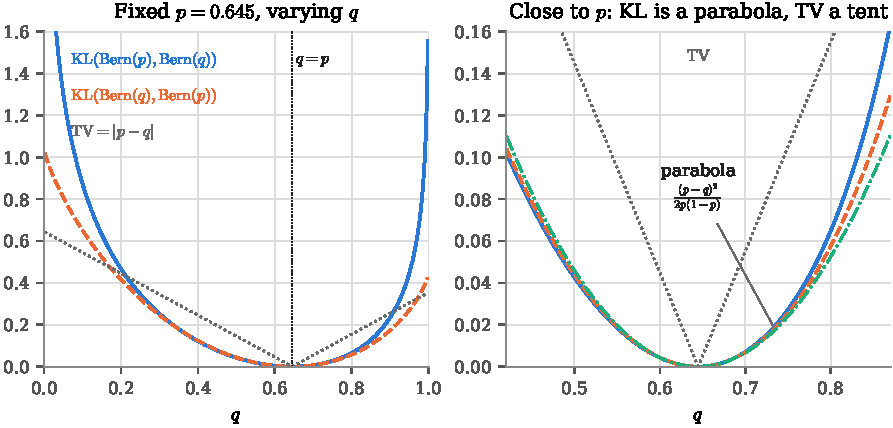
\includegraphics[width=\textwidth]{fig_kl_bernoulli}
\caption{KL divergence and total variation between $\Bern(p)$ and $\Bern(q)$, with $p = 0.645$ fixed and $q$ varying. Left, the whole range: total variation is a tent with straight sides; the two KL divergences are smooth at $q = p$, differ from each other away from it, and $\KL(\Bern(p), \Bern(q))$ (blue) goes to infinity as $q$ approaches $0$ or $1$, where $\Bern(q)$ calls one of the two outcomes impossible. Right, near $q = p$: both KL curves hug the parabola $(p - q)^2 / (2p(1-p))$. At $q = \frac12$: total variation $0.145$, the two KL divergences $0.0428$ and $0.0440$, the parabola $0.0460$.}
\label{fig:klbern}
\end{figure}

\begin{worked}[KL divergences you can compute by hand]
\begin{itemize}
\item \textbf{Two Bernoullis.} With two outcomes the sum has two terms:
\[
\KL(\Bern(p), \Bern(q)) = p \log \frac{p}{q} + (1 - p) \log \frac{1 - p}{1 - q}.
\]
\Cref{fig:klbern} plots it with $p = 0.645$ fixed.
Two values to keep: $\KL(\Bern(\frac12), \Bern(\frac1{10})) = 0.511$ and $\KL(\Bern(\frac1{10}), \Bern(\frac12)) = 0.368$.
\item \textbf{Two Gaussians with the same variance.} For $\Pr = \Gauss(a, \sigma^2)$ and $\Qr = \Gauss(b, \sigma^2)$ the normalizing constants cancel in the ratio, and
\[
\log \frac{p(x)}{q(x)} = \frac{(x - b)^2 - (x - a)^2}{2\sigma^2} = \frac{(a - b)(2x - a - b)}{2\sigma^2}.
\]
This is linear in $x$, so its expectation under $X \sim \Gauss(a, \sigma^2)$ is the same expression at $x = a$:
\[
\KL(\Gauss(a, \sigma^2), \Gauss(b, \sigma^2)) = \frac{(a - b)(2a - a - b)}{2\sigma^2} = \frac{(a - b)^2}{2\sigma^2}.
\]
Half the squared distance between the means in standard-deviation units. For the left pair of \cref{fig:paramvsdist}, means $0$ and $0.01$ with $\sigma = 1$ give $0.00005$. The right pair, standard deviations $0.01$ and $0.02$, does not have a common variance and needs the general formula of \cref{ex:dist-kl-gauss}: $\KL(\Gauss(0, 0.01^2), \Gauss(0, 0.02^2)) = 0.318$, and $0.807$ the other way.
\item \textbf{Two exponentials.} For $\Expo(\lambda)$ against $\Expo(\mu)$, $\log(p(x)/q(x)) = \log(\lambda/\mu) - (\lambda - \mu)x$, again linear in $x$, with $\E[X] = 1/\lambda$:
\[
\KL(\Expo(\lambda), \Expo(\mu)) = \log \frac{\lambda}{\mu} - \frac{\lambda - \mu}{\lambda} = \log\frac{\lambda}{\mu} + \frac{\mu}{\lambda} - 1.
\]
$\KL(\Expo(1), \Expo(2)) = 0.307$ and $\KL(\Expo(2), \Expo(1)) = 0.193$.
\end{itemize}
\end{worked}

\begin{sanitycheck}[The Gaussian formula]
Check $(a - b)^2/(2\sigma^2)$ three ways.
At $a = b$ it is $0$, which a divergence between a distribution and itself must be.
It is symmetric in $a$ and $b$, which is right here (swapping the two Gaussians is the same as reflecting the line, and reflecting changes nothing), though KL is not symmetric in general.
And it is unchanged if $a$, $b$ and $\sigma$ are all converted to a new unit, say minutes instead of hours: a divergence between distributions can't depend on the units of the measurement, and $(a - b)/\sigma$ doesn't.
\end{sanitycheck}

\begin{proposition}[Properties of the KL divergence]
\label{prop:kl-properties}
For distributions $\Pr$ and $\Qr$ on $E$:
\begin{enumerate}[nosep]
\item \textbf{nonnegativity:} $\KL(\Pr, \Qr) \geq 0$;
\item \textbf{definiteness:} $\KL(\Pr, \Qr) = 0$ only if $\Pr = \Qr$;
\item \textbf{no symmetry:} in general $\KL(\Pr, \Qr) \neq \KL(\Qr, \Pr)$;
\item \textbf{no triangle inequality:} in general $\KL(\Pr, \Qr) \not\leq \KL(\Pr, \mathbb{V}) + \KL(\mathbb{V}, \Qr)$.
\end{enumerate}
Properties 1 and 2 make KL behave like a distance in the way that matters most: it is zero exactly when the distributions agree. Properties 3 and 4 mean it is not a distance, which is why it is called a divergence.
\end{proposition}

\coreproof{The log-ratio $\log(p/q)$ is $-\log$ of the ratio $q/p$. The curve $-\log y$ lies above its tangent line $1 - y$ at $y = 1$, touching it only there. The average of the ratio $q(X)/p(X)$ under $\Pr$ is at most $1$, since it is the total mass of $q$ on the points where $p$ is positive, so the average of the tangent line is at least $0$.}
\begin{proof}
(1) If $\KL(\Pr, \Qr) = +\infty$ there is nothing to prove, so assume $q > 0$ wherever $p > 0$.
Let $X \sim \Pr$ and $Y = q(X)/p(X)$, a positive random variable.
Then $\log(p(X)/q(X)) = -\log Y$.
The function $g(y) = -\log y$ is convex ($g''(y) = 1/y^2 > 0$), so it lies above its tangent line at $y = 1$, which is $1 - y$, and touches it only at $y = 1$ \toolkit{sec:math-convex}:
\[
-\log y \geq 1 - y \quad \text{for all } y > 0, \text{ with equality only at } y = 1.
\]
Taking expectations,
\[
\KL(\Pr, \Qr) = \E[-\log Y] \geq 1 - \E[Y].
\]
In the discrete case, $\E[Y] = \sum_{x: p(x) > 0} p(x) \cdot q(x)/p(x) = \sum_{x: p(x) > 0} q(x) \leq 1$; in the continuous case the same with an integral.
So $1 - \E[Y] \geq 0$. (This is the same idea as Jensen's inequality, \cref{thm:jensen}: the tangent-line argument is its proof.)

(2) If $\KL(\Pr, \Qr) = 0$, both inequalities in (1) are equalities.
The first, $\E[-\log Y] = 1 - \E[Y]$, is an average of the nonnegative gap $-\log Y - (1 - Y)$ that comes out $0$, so the gap is $0$ with probability $1$, which forces $Y = 1$: $q(x) = p(x)$ at every point where $p(x) > 0$.
Then $q$ already has total mass $1$ on those points, so it has none anywhere else, and $q = p$.

(3) $\KL(\Bern(\frac12), \Bern(\frac1{10})) = 0.511$ and $\KL(\Bern(\frac1{10}), \Bern(\frac12)) = 0.368$.

(4) With the Gaussian formula,
\[
\begin{aligned}
\KL(\Gauss(0,1), \Gauss(2,1)) &= 2, \quad \text{while}\\
\KL(\Gauss(0,1), \Gauss(1,1)) + \KL(\Gauss(1,1), \Gauss(2,1)) &= 0.5 + 0.5 = 1.
\end{aligned}
\]
The direct route is twice as long as the detour: KL grows like a squared distance, and squares of distances don't satisfy the triangle inequality.
\end{proof}

\begin{intuition}[why the order matters: who is surprised by what]
Think of $\log(1/q(x))$ as how surprised you are to see $x$ if you believe $\Qr$.
Then $\KL(\Pr, \Qr)$ is how much more surprised, on average, a believer in $\Qr$ is than a believer in $\Pr$, when the data really come from $\Pr$.
Take $\Pr = \Bern(\frac12)$, a fair coin, and $\Qr = \Bern(\frac1{10})$, a coin that rarely shows heads.
With the fair coin as the truth, each head is $5$ times likelier under the truth than under $\Qr$, worth $\log 5 = 1.609$ in favor of the truth, and heads come half the time; each tail favors $\Qr$ by $\log(0.9/0.5) = 0.588$.
On average, $0.5 \times 1.609 - 0.5 \times 0.588 = 0.511$.
Reverse the roles, so the $\frac1{10}$ coin is the truth.
Now each tail favors the truth by $0.588$ and comes $90\%$ of the time, while the rare heads favor the fair-coin believer by $1.609$: on average $0.9 \times 0.588 - 0.1 \times 1.609 = 0.368$.
The decisive outcome, heads, is common in the first case and rare in the second.
The divergence is largest when the alternative calls rare what the truth makes common.
At the extreme, $\KL(\Bern(\frac12), \Bern(0)) = +\infty$, since the first head refutes `heads never happen'; but $\KL(\Bern(0), \Bern(\frac12)) = \log 2 = 0.693$, finite, since a stream of tails is perfectly possible for a fair coin, just less likely each time.
\end{intuition}

\subsection{Independent observations add}

The single most useful property of the KL divergence is the one total variation lacks.

\begin{proposition}[Additivity over independent observations]
\label{prop:kl-additive}
If $\Pr^{\otimes n}$ and $\Qr^{\otimes n}$ denote the distributions of $n$ independent draws from $\Pr$ and from $\Qr$, then
\[
\KL(\Pr^{\otimes n}, \Qr^{\otimes n}) = n \, \KL(\Pr, \Qr).
\]
\end{proposition}

\optionalproof{The log of a product is a sum, and an expectation of a sum is a sum of expectations.}
\begin{proof}
The joint PMF or density of $n$ independent draws is the product, so the log-ratio of the joint distributions is a sum:
\[
\log \frac{\prod_{i=1}^n p(x_i)}{\prod_{i=1}^n q(x_i)} = \sum_{i=1}^n \log \frac{p(x_i)}{q(x_i)}.
\]
Under $\Pr^{\otimes n}$ each $X_i \sim \Pr$, and the expectation of a sum is the sum of the expectations, each equal to $\KL(\Pr, \Qr)$.
\end{proof}

Evidence from independent observations accumulates, and on the log scale it accumulates by addition.
For the kiss data, $124$ couples supply on average $124 \times 0.0428 = 5.30$ nats of evidence for $p = 0.645$ over $p = \frac12$, a likelihood ratio of about $e^{5.30} \approx 200$.
The count of right turns is enough to compute that evidence, so the same additivity gives $\KL(\Bin(n, p), \Bin(n, q)) = n\, \KL(\Bern(p), \Bern(q))$, which \cref{ex:dist-kl-binomial} asks you to check directly.
Compare total variation, which went from $0.145$ for one couple to $0.900$ for $124$, by no rule you could state, and could never pass $1$.

\subsection{Near the truth, KL is a parabola}

\Cref{fig:klbern} shows something about the shape of KL that the formulas don't make obvious.
Total variation between Bernoullis is $\abs{p - q}$, a tent with a corner at $q = p$.
KL is smooth there: flat at the bottom, curving up on both sides, the shape of a parabola.
It must be flat at $q = p$, since KL has a minimum of $0$ there and is differentiable.
A second-order Taylor expansion \toolkit{sec:math-mvt} in $q$ around $p$ gives the curvature.
With $f(q) = p \log(p/q) + (1-p)\log((1-p)/(1-q))$, $f(p) = 0$; $f'(q) = -p/q + (1-p)/(1-q)$, so $f'(p) = 0$; and $f''(q) = p/q^2 + (1-p)/(1-q)^2$, so $f''(p) = 1/p + 1/(1-p) = 1/(p(1-p))$.
Hence
\[
\KL(\Bern(p), \Bern(q)) \approx \frac12 f''(p) (q - p)^2 = \frac{(p - q)^2}{2p(1 - p)} \quad \text{for $q$ near $p$}.
\]
For the kiss data the approximation gives $0.0460$ against the exact $0.0428$.

Look at what the curvature is: $1/(p(1-p))$, one over the variance of a single Bernoulli observation.
The Gaussian formula has the same shape, $(a - b)^2/(2\sigma^2)$, with curvature $1/\sigma^2$.
In both, KL near the truth is half the squared parameter distance measured in units of the noise in one observation.
Where an observation is noisy, nearby parameters are hard to tell apart and KL rises slowly; where it is precise, KL rises fast.
\Cref{ch:mle-properties} gives the curvature its name, the Fisher information, and shows that it sets the variance of the best estimators.

\begin{bridge}[the $G$-test and Pearson's chi-squared]
Some introductory courses teach a test of a proportion, or of a table of counts, called the $G$-test or likelihood-ratio chi-squared test: $G^2 = 2\sum O \log(O/E)$, summed over cells, with $O$ the observed and $E$ the expected counts.
That statistic is a KL divergence.
For the kiss data, the cells are right and left, $O = (80, 44)$ and, under $p = \frac12$, $E = (62, 62)$:
\[
G^2 = 2\left(80 \log \tfrac{80}{62} + 44 \log \tfrac{44}{62}\right) = 2 \times 124 \times \KL\big(\Bern(\hat{p}), \Bern(\tfrac12)\big) = 10.60,
\]
twice the $5.30$ nats of evidence above.
Pearson's chi-squared statistic for the same table is $\sum (O - E)^2/E = 10.45$, which is also $z^2 = 3.233^2$ from the test of \cref{sec:tests-kiss}.
Pearson's statistic is a parabola approximation to $G^2$, with the variance taken at the null value.
The expansion above was in $q$ around $p$; expanding instead in $p$ around $q$ gives the same parabola with the variance at $q$, $(p - q)^2/(2q(1 - q))$.
With $q = \frac12$ that is $2(\hat{p} - \frac12)^2 = 0.0421$, and $248 \times 0.0421 = 10.45$, Pearson's statistic.
With the variance at $\hat{p}$ instead, $248 \times 0.0460 = 11.41$, the square of the Wald statistic $\sqrt{124}(\hat{p} - \frac12)/\sqrt{\hat{p}(1 - \hat{p})} = 3.38$ of \cref{ch:wald-lrt}.
Both are compared with a chi-squared distribution with one degree of freedom, whose $95\%$ quantile is $3.84 = 1.96^2$, and both reject.
\Cref{ch:gof} develops the chi-squared test in general.
\end{bridge}

\subsection{KL controls total variation}

KL is not a distance, but small KL forces small total variation.

\begin{theorem}[Pinsker's inequality]
\label{thm:pinsker}
For any distributions $\Pr$ and $\Qr$,
\[
\TV(\Pr, \Qr) \leq \sqrt{\tfrac12 \KL(\Pr, \Qr)}.
\]
\end{theorem}

Nothing later in the book depends on Pinsker's inequality, so its proof is in \cref{sec:proof-pinsker} of \cref{app:proofs}. It is a page of calculus that reuses the tangent-line bound from the proof of \cref{prop:kl-properties}.
For the kiss data, $\sqrt{0.0428/2} = 0.146$, against $\TV = 0.145$: nearly tight.
The inequality is what lets you work with KL, which is convenient, and still conclude something about total variation, which is what you wanted in \cref{sec:dist-close}: if the fitted distribution is close to the truth in KL, then every probability it reports is close to the true probability.
The converse fails: total variation can be small while KL is infinite.
$\Pr = \Pois(1/n)$ and $\Qr$, the distribution that puts all its mass at $0$, have $\TV = 1 - e^{-1/n}$, which goes to $0$, while $\KL(\Pr, \Qr) = +\infty$ for every $n$, since $\Pr$ gives positive probability to $1$ and $\Qr$ calls it impossible (\cref{ex:dist-pois-dirac}).

\section{Estimating the KL divergence: the road to maximum likelihood}
\label{sec:dist-estimating-kl}

Return to the plan of \cref{sec:dist-tv-estimate} with KL in place of total variation.
The quantity to make small is $\theta \mapsto \KL(\Pr_{\theta^*}, \Pr_\theta)$, the divergence of the candidate from the truth.
The truth goes first: the average is taken under the distribution the data come from, which is the only distribution you can average under.
Split the logarithm of the ratio into a difference:
\[
\KL(\Pr_{\theta^*}, \Pr_\theta) = \E_{\theta^*}\big[\log p_{\theta^*}(X)\big] - \E_{\theta^*}\big[\log p_\theta(X)\big].
\]
The first term involves the unknown $\theta^*$, but it does not involve $\theta$: as a function of $\theta$ it is a constant.
The second term is an expectation under the truth of a function, $\log p_\theta$, that you can compute for any $\theta$ you like.

\recall{The Law of Large Numbers (\cref{thm:wlln}): an average of $h(X_1), \ldots, h(X_n)$ over iid data converges in probability to $\E_{\theta^*}[h(X)]$, provided $h(X)$ has finite variance.}

Apply it to $h = \log p_\theta$, one $\theta$ at a time:
\[
\widehat{\KL}(\Pr_{\theta^*}, \Pr_\theta) = \text{constant} - \frac1n \sum_{i=1}^n \log p_\theta(X_i).
\]
You don't know the constant, and you don't need to.
The $\theta$ that minimizes $\widehat{\KL}$ is the same whatever the constant is, and it is the $\theta$ that maximizes $\frac1n \sum_i \log p_\theta(X_i)$.
Since $\log$ turns a product into a sum and is increasing \toolkit{sec:math-explog},
\[
\operatorname*{argmin}_\theta \widehat{\KL}(\Pr_{\theta^*}, \Pr_\theta) = \operatorname*{argmax}_\theta \sum_{i=1}^n \log p_\theta(X_i) = \operatorname*{argmax}_\theta \prod_{i=1}^n p_\theta(X_i).
\]
The product $\prod_i p_\theta(X_i)$ is the probability, or density, of the data you observed, computed as if $\theta$ were the truth.
The $\theta$ that makes your data most probable is the \textbf{maximum likelihood estimator}, and minimizing the estimated KL divergence is the same thing as finding it.
\Cref{ch:likelihood} takes this as its starting point.

\begin{worked}[the kiss data]
For Bernoulli data, $\log p_q(x) = x \log q + (1 - x)\log(1 - q)$, and the average over $124$ couples of whom $80$ turned right is
\[
\frac{1}{124}\sum_{i=1}^{124} \log p_q(R_i) = \hat{p} \log q + (1 - \hat{p}) \log(1 - q), \qquad \hat{p} = \tfrac{80}{124} = 0.645.
\]
Its derivative in $q$ is $\hat{p}/q - (1 - \hat{p})/(1 - q)$, which is zero at $q = \hat{p}$, positive before and negative after.
The estimated KL is smallest at the sample proportion, $\hat{p} = 0.645$, the estimator you would have used anyway.
\end{worked}

\Cref{fig:klestimate} shows the estimate at work.
To draw it, the unknown constant has to be filled in, so the figure does what only a simulation can: it fixes the truth at $p^* = 0.645$ and draws samples from it.
The black curve is the true $\KL(\Bern(p^*), \Bern(q))$.
Each colored curve is the estimate from one simulated sample, $\frac1n \sum_i \log(p^*(R_i)/p_q(R_i))$, the same curve as the true one with the expectation replaced by an average.
Each estimated curve has its minimum at its own sample proportion.
As $n$ grows the estimated curves close in on the true one, and their minimizers close in on $p^*$, which is the true curve's minimizer.
That is the argument \cref{ch:mle-properties} turns into a proof that the maximum likelihood estimator is consistent.

\begin{figure}[htbp]
\centering
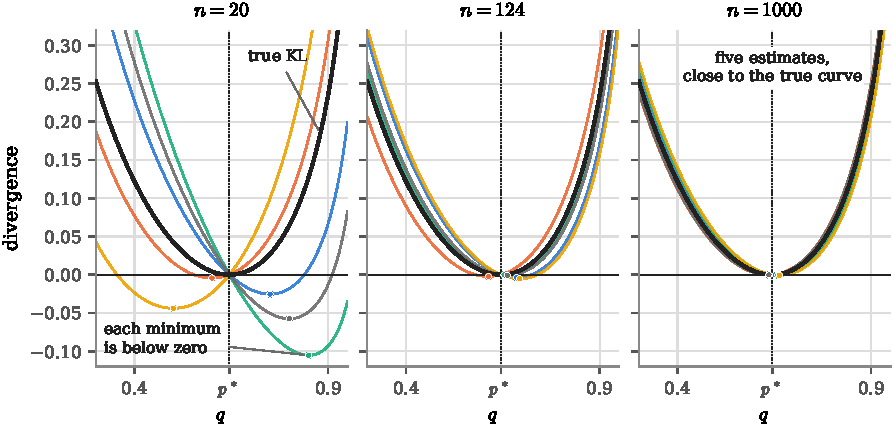
\includegraphics[width=\textwidth]{fig_kl_estimate}
\caption{The true $\KL(\Bern(p^*), \Bern(q))$ for $p^* = 0.645$ (black) and five estimates of it, each from one simulated sample of $n$ couples (colors), for $n = 20$, $124$ and $1{,}000$. Each estimated curve is lowest at its own sample proportion (dots), which is the maximum likelihood estimate. Every estimated curve passes through $0$ at $q = p^*$ and dips below zero near its minimum. As $n$ grows the estimates close in on the true curve, and their minimizers on $p^*$.}
\label{fig:klestimate}
\end{figure}

\begin{sanitycheck}[An estimated divergence below zero]
Every estimated curve in \cref{fig:klestimate} dips below zero, and a KL divergence is never negative.
Is the estimate broken?
No.
At $q = p^*$ the estimate is exactly $0$ (each term is $\log 1$), and at its own minimizer $\hat{p}$ it must be lower still.
The estimate is an average, and an average of quantities whose expectation is positive can come out negative in a finite sample; the LLN promises only that it ends up near the expectation.
What the dip measures is how much better the sample proportion fits this sample than the truth does, which is always at least a little, since $\hat{p}$ was chosen by looking at the sample.
For $n = 20$ the dips are visible; for $n = 1{,}000$ they are invisible at this scale.
\end{sanitycheck}

\begin{pitfall}[the constant you dropped was the distance]
Minimizing $\widehat{\KL}$ finds the best $\theta$, but the minimum value of $-\frac1n\sum_i \log p_\theta(X_i)$ is not an estimate of the distance from the truth.
The dropped constant $\E_{\theta^*}[\log p_{\theta^*}(X)]$ is unknown, so the number you computed is the divergence plus an unknown shift.
The maximized log-likelihood of the kiss data, $80 \log 0.645 + 44 \log 0.355 = -80.6$, says nothing on its own about how well the Bernoulli model fits.
Only differences of log-likelihoods, between two values of $\theta$ or two models fitted to the same data, cancel the constant and mean something.
That is why the likelihood ratio tests of \cref{ch:wald-lrt} compare two maximized log-likelihoods and never interpret one alone.
\end{pitfall}

\section{When the model is wrong: the closest member of the family}
\label{sec:dist-projection}

Everything so far assumed the truth is $\Pr_{\theta^*}$ for some $\theta^*$ in the model.
\Cref{ch:models} warned that the assumption can fail, and promised to say what estimators estimate when it does.
Here is the answer.

Let the truth be any distribution $\Pr$, in the family or not.
\recall{The Law of Large Numbers (\cref{thm:wlln}): for iid data from $\Pr$, $\frac1n \sum_i h(X_i) \convp \E_\Pr[h(X)]$ when $h(X)$ has finite variance. Nothing in it requires $\Pr$ to belong to a model.}
The estimated divergence is built the same way: $\KL(\Pr, \Pr_\theta) = \E_{\Pr}[\log p(X)] - \E_{\Pr}[\log p_\theta(X)]$, the first term is still a constant, and the LLN still estimates the second by $\frac1n\sum_i \log p_\theta(X_i)$, since the data still come from $\Pr$.
So maximum likelihood still minimizes an estimate of $\theta \mapsto \KL(\Pr, \Pr_\theta)$.
What has changed is the minimum: no $\theta$ makes the divergence $0$, so the minimizer is the member of the family that is closest to the truth, not the truth.

\begin{definition}[KL projection]
\label{def:kl-projection}
Let $\Pr$ be a distribution and $(\Pr_\theta)_{\theta \in \Theta}$ a family on the same sample space.
A \textbf{KL projection} of $\Pr$ onto the family is a parameter
\[
\theta^\circ = \operatorname*{argmin}_{\theta \in \Theta} \KL(\Pr, \Pr_\theta),
\]
when the minimum exists and is attained at a single point.
If $\Pr = \Pr_{\theta^*}$ is in the family and the model is identifiable, $\theta^\circ = \theta^*$.
\end{definition}

\begin{inwords}
\textbf{In words.} Look over every distribution the model allows and pick the one the truth diverges from least. If the truth is in the model, that is the truth itself, at divergence $0$. If not, it is the model's best impersonation of the truth. Maximum likelihood, applied to data from a truth outside the model, estimates $\theta^\circ$: under conditions that \cref{ch:mle-properties} states, $\hat{\theta}_n \convp \theta^\circ$. So a wrong model fitted by maximum likelihood is not meaningless. It converges to something definite, the closest member of the family, and the question is only whether the closest member is close enough for your purpose.
\par\smallskip
\textbf{For the kiss data.} The Bernoulli family contains every distribution on $\{0, 1\}$, so for the kiss experiment the model cannot be wrong in this sense: whatever the truth is, one couple's turn is some $\Bern(p)$. What can fail is the iid assumption of \cref{ch:kiss}: couples influencing each other, or one observer's couples differing from another's. A Bernoulli model with dependent data is misspecified in a way that no projection onto a family of iid models repairs.
\end{inwords}

\begin{proposition}[KL projection onto the Gaussian and Poisson families]
\label{prop:kl-projection}
Let $\Pr$ be the distribution of a random variable $X$.
\begin{enumerate}[nosep]
\item If $X$ has a density $p$ with $\E\abs{\log p(X)} < \infty$ and finite variance, the KL projection onto $(\Gauss(\mu, \sigma^2))_{\mu \in \real, \sigma^2 > 0}$ is $\mu^\circ = \E[X]$, $(\sigma^2)^\circ = \var(X)$: the Gaussian with the same mean and variance.
\item If $X$ takes values in $\{0, 1, 2, \ldots\}$, with $\E[X] > 0$, $\E[\log X!] < \infty$ and $\E\abs{\log p(X)} < \infty$ for its PMF $p$, the KL projection onto $(\Pois(\lambda))_{\lambda > 0}$ is $\lambda^\circ = \E[X]$: the Poisson with the same mean.
\end{enumerate}
\end{proposition}

The conditions on $\log p(X)$ keep the constant $\E[\log p(X)]$ finite. Without them the divergence can be $+\infty$ for every member of the family (a discrete $X$ against any Gaussian, say), and what maximum likelihood targets is then the minimizer of $-\E[\log p_\theta(X)]$ alone, which the same calculation finds.

\optionalproof{Only the term $-\E[\log p_\theta(X)]$ depends on the parameter. For both families it involves $X$ only through $\E[X]$ and $\E[X^2]$ (plus a term free of the parameter), so it is an explicit function of the parameters. Minimize it by calculus.}
\begin{proof}
(1) For the Gaussian density, $-\log p_{\mu, \sigma^2}(x) = \frac12 \log(2\pi\sigma^2) + (x - \mu)^2/(2\sigma^2)$, and
\[
-\E[\log p_{\mu,\sigma^2}(X)] = \tfrac12 \log(2\pi\sigma^2) + \frac{\E[(X - \mu)^2]}{2\sigma^2} = \tfrac12 \log(2\pi\sigma^2) + \frac{\var(X) + (\E[X] - \mu)^2}{2\sigma^2},
\]
using the bias-variance split $\E[(X - \mu)^2] = \var(X) + (\E[X] - \mu)^2$ from \cref{ch:estimators}.
For any $\sigma^2$, the $\mu$ that minimizes this is $\mu = \E[X]$, which kills the squared term.
With that $\mu$, the derivative in $\sigma^2$ of $\frac12\log(2\pi\sigma^2) + \var(X)/(2\sigma^2)$ is $\frac{1}{2\sigma^2} - \frac{\var(X)}{2\sigma^4}$, zero at $\sigma^2 = \var(X)$, negative before and positive after, so this is the minimum.

(2) For the Poisson PMF, $-\log p_\lambda(x) = \lambda - x\log\lambda + \log(x!)$, and $-\E[\log p_\lambda(X)] = \lambda - \E[X] \log\lambda + \E[\log X!]$.
The last term doesn't depend on $\lambda$.
The derivative of the rest is $1 - \E[X]/\lambda$, zero at $\lambda = \E[X]$, negative before and positive after.
\end{proof}

\begin{worked}[fitting a Gaussian to exponential data]
Let the truth be $\Expo(1)$, which has mean $1$ and variance $1$, and fit the Gaussian family.
The KL projection is $\Gauss(1, 1)$.
From the proof, with $\var(X) = 1$ and $\E[X] = 1$, and with the constant term $\E[\log e^{-X}] = -\E[X] = -1$,
\[
\KL(\Expo(1), \Gauss(\mu, \sigma^2)) = \tfrac12\log(2\pi\sigma^2) + \frac{1 + (1 - \mu)^2}{2\sigma^2} - 1.
\]
At the projection the divergence is $\frac12\log(2\pi) + \frac12 - 1 = 0.419$.
The minimum is not $0$, since no Gaussian is an exponential.
\Cref{fig:klprojection} shows the projection against two other candidates, $\Gauss(0.7, 0.6)$, which is taller and sits closer to the exponential's peak at $0$, and $\Gauss(1.5, 1.5)$, which covers its long right tail better.
Both diverge more, $0.572$ and $0.538$.
The divergence weights each point by how often the truth produces it, and it penalizes a candidate that calls likely outcomes unlikely; matching the mean and the variance is the best a Gaussian can do on that criterion.
\end{worked}

\begin{figure}[htbp]
\centering
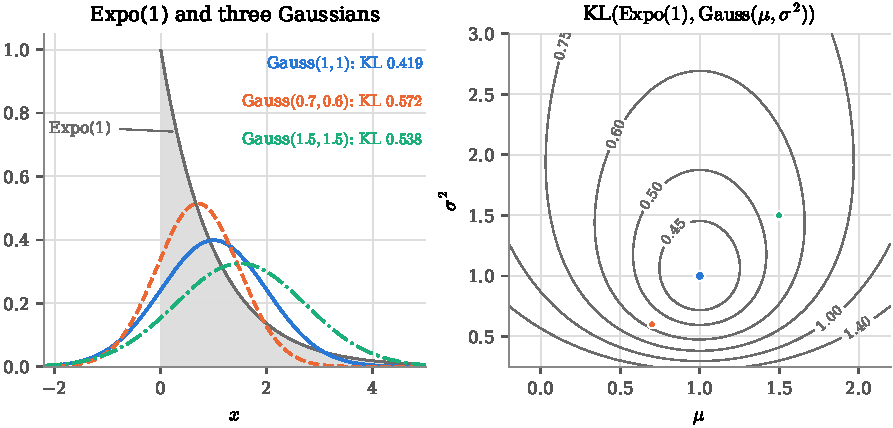
\includegraphics[width=\textwidth]{fig_kl_projection}
\caption{Projecting $\Expo(1)$ onto the Gaussian family. Left: the exponential density (gray) and three Gaussians with their KL divergences from it. Right: $\KL(\Expo(1), \Gauss(\mu, \sigma^2))$ over a grid of means and variances, with its minimum $0.419$ at mean $1$ and variance $1$, the exponential's own mean and variance; the dots mark the three Gaussians on the left.}
\label{fig:klprojection}
\end{figure}

The Poisson half of \cref{prop:kl-projection} pays off the debt of \cref{ch:models}.
The siblings data of \cref{fig:siblings} were fitted with $X - 1 \sim \Pois(\hat{\lambda})$ and $\hat{\lambda}$ the sample mean minus one.
If the true distribution of the number of siblings is not a shifted Poisson, say with an extra bump at $5$, the fit is still estimating something definite: the shifted Poisson whose mean matches the true mean, $\lambda^\circ = \E[X] - 1$, which is the KL projection.
The sample mean minus one estimates it by the LLN, which needs no assumption that the shifted Poisson is right.
Whether that projection is a good description of the truth is a separate question, and it is the question the goodness-of-fit tests of \cref{ch:gof} ask.

\begin{bridge}[`fit a normal with the sample mean and standard deviation']
An introductory course fits a normal distribution to data by plugging in $\bar{x}$ and $s$, and justifies it, if at all, by saying that the normal is determined by its mean and standard deviation.
\Cref{prop:kl-projection} is a better justification, and it holds whether or not the data are normal: $\Gauss(\E[X], \var(X))$ is the Gaussian closest to the truth in KL, and $\bar{x}$ and $s^2$ estimate its two parameters.
What the procedure can't tell you is whether the closest Gaussian is close.
For exponential data it is $0.419$ nats away, and probabilities computed from it can be badly wrong: under $\Gauss(1, 1)$ the probability of a negative value is $\Phi(-1) = 0.16$, under $\Expo(1)$ it is $0$.
A QQ plot (\cref{ch:ks}) is how you see that in data.
\end{bridge}

\begin{pitfall}[the order of the arguments is not a choice]
$\KL(\Pr, \Pr_\theta)$ and $\KL(\Pr_\theta, \Pr)$ are different functions of $\theta$ with different minimizers in general.
Statistics minimizes the first, with the truth first, and not because it is better in some abstract sense: it is the only one that can be estimated.
The first is an expectation under the truth $\Pr$, which the data average.
The second is an expectation under the candidate $\Pr_\theta$, and it has the unknown $p$ inside it in a way that does not split off as a constant.
Because KL is not symmetric, the two orders are different problems, and only the truth-first order is an average under the distribution the data come from.
\end{pitfall}

\section{What comes next}
\label{sec:dist-next}

This chapter ended at maximum likelihood without defining a likelihood.
\Cref{ch:likelihood} defines it, for discrete and continuous models, and computes the maximum likelihood estimator for the families of this book: Bernoulli, Poisson, Gaussian, exponential, uniform.
\Cref{ch:mle-properties} proves what \cref{fig:klestimate} shows, that the estimator converges to the minimizer of the KL divergence, and then uses the curvature of KL at its minimum, the $1/(p(1-p))$ of \cref{fig:klbern}, to find its asymptotic variance: that curvature is the Fisher information.
Distances between distributions return in \cref{ch:ks}, where the largest gap between an empirical CDF and a candidate CDF is the test statistic.

\section{Summary}
\label{sec:dist-summary}

\begin{itemize}[nosep]
\item Closeness should be measured between distributions, not parameters: a parameter difference of $0.01$ is $\TV = 0.004$ for two means with $\sigma = 1$ and $\TV = 0.323$ for standard deviations $0.01$ and $0.02$. A distance between distributions also makes sense when the model is wrong.
\item Total variation: $\TV(\Pr, \Qr) = \max_A \abs{\Pr(A) - \Qr(A)} = \frac12 \sum \abs{p - q}$ (or $\frac12\int$), attained at $\{p > q\}$; the area where one density is above the other; $1 - \TV$ is the shared mass. A true distance with values in $[0, 1]$. $\TV(\Bern(p), \Bern(q)) = \abs{p - q}$; kiss data $0.145$ for one couple, $0.900$ for $124$.
\item The best test of $\Pr$ against $\Qr$ has $\alpha + \beta = 1 - \TV$. For $124$ couples it rejects $p = \frac12$ from $72$ right turns, with $\alpha = 0.0438$ and $\beta = 0.0567$.
\item Total variation ignores the geometry of the sample space: $\TV(X, X + 0.001) = 1$, and a discrete distribution is at distance $1$ from every continuous one, so the CLT is not convergence in total variation.
\item Total variation can't be estimated by an average: written as an expectation under the truth, it has the unknown density inside an absolute value. Plugging in frequencies works for a few discrete outcomes and fails for continuous data.
\item KL divergence: $\KL(\Pr, \Qr) = \E_\Pr[\log(p(X)/q(X))]$, the average evidence per observation for $\Pr$ over $\Qr$; $+\infty$ if $\Qr$ calls impossible what $\Pr$ produces. Nonnegative and zero only for $\Pr = \Qr$ (Jensen), but not symmetric and no triangle inequality. Kiss data: $0.0428$ and, reversed, $0.0440$.
\item Formulas: Bernoulli $p\log(p/q) + (1-p)\log((1-p)/(1-q))$; Gaussians with a common variance $(a - b)^2/(2\sigma^2)$; exponentials $\log(\lambda/\mu) + \mu/\lambda - 1$.
\item KL adds over independent observations: $\KL(\Pr^{\otimes n}, \Qr^{\otimes n}) = n \KL(\Pr, \Qr)$; $124 \times 0.0428 = 5.30$ nats for the kiss data. Near the truth it is a parabola with curvature one over the variance of one observation, $(p - q)^2/(2p(1-p))$ for Bernoulli. $2n\KL$ is the $G^2$ statistic, and its parabola approximation is Pearson's chi-squared.
\item Pinsker: $\TV \leq \sqrt{\KL/2}$; the converse fails.
\item $\KL(\Pr_{\theta^*}, \Pr_\theta)$ is a constant minus $\E_{\theta^*}[\log p_\theta(X)]$, and the LLN estimates the second term by $\frac1n \sum \log p_\theta(X_i)$. Minimizing the estimate is maximizing the likelihood $\prod p_\theta(X_i)$. Kiss data: the minimizer is $\hat{p} = 0.645$.
\item When the model is wrong, maximum likelihood estimates the KL projection, the member of the family closest to the truth. For the Gaussian family it has the true mean and variance; for the Poisson family, the true mean. $\Expo(1)$ projects to $\Gauss(1,1)$ at divergence $0.419$.
\end{itemize}

\section{Exercises}
\label{sec:dist-exercises}

\begin{exercise}
\label{ex:dist-tv-bern}
Compute $\TV(\Bern(\frac12), \Bern(\frac12))$, $\TV(\Bern(\frac12), \Bern(\frac13))$ and $\TV(\Bern(\frac12), \Bern(\frac1{10}))$ from \cref{def:tv}, by listing the events, and check each against the formula $\abs{p - q}$.
\end{exercise}
\begin{solution}
On $E = \{0, 1\}$ the events are $\emptyset$, $\{0\}$, $\{1\}$ and $E$, and the first and last have the same probability under any two distributions. For $\Bern(\frac12)$ against $\Bern(q)$, the event $\{1\}$ has probabilities $\frac12$ and $q$, and $\{0\}$ has $\frac12$ and $1 - q$; both differences are $\abs{\frac12 - q}$. So the three distances are $0$, $\frac16 = 0.167$ and $0.4$, matching $\abs{p - q}$. The first is $0$ whether or not two Bernoulli variables with these distributions are independent: total variation compares distributions, not random variables, and their joint behavior doesn't enter.
\end{solution}

\begin{exercise}
\label{ex:dist-tv-expo-unif}
Show that $\TV(\Expo(1), \Unif([0,1])) = 1/e$, and identify the event $A^\star$ of \cref{prop:tv-area}.
\end{exercise}
\begin{solution}
The computation is the third item of the worked example in \cref{sec:dist-tv}. The event on which $\Expo(1)$ puts more mass is $A^\star = \{x > 1\}$, where the uniform density is $0$; its probabilities are $e^{-1}$ and $0$, so $\abs{\Pr(A^\star) - \Qr(A^\star)} = e^{-1} = 0.368$, the same answer as the integral. The complementary event $[0, 1]$ favors the uniform by the same amount, $1 - (1 - e^{-1}) = e^{-1}$.
\end{solution}

\begin{exercise}
\label{ex:dist-tv-shift}
Let $X \sim \Bern(\frac12)$ and $a \in (0, 1)$. Show that $\TV(X, X + a) = 1$, meaning the total variation distance between the distributions of $X$ and $X + a$. Then show that $\TV(2\sqrt{n}(\bar{X}_n - \frac12), Z) = 1$ for every $n$, where $\Xton \iid \Bern(\frac12)$ and $Z \sim \Gauss(0,1)$, and explain why this does not contradict the CLT.
\end{exercise}
\begin{solution}
$X$ takes values in $\{0, 1\}$ and $X + a$ in $\{a, 1 + a\}$, disjoint from it since $0 < a < 1$. The event $A = \{0, 1\}$ has $\Pr(X \in A) = 1$ and $\Pr(X + a \in A) = 0$, so $\TV = 1$, the largest possible value. For the second, $2\sqrt{n}(\bar{X}_n - \frac12)$ takes values in the finite set $S_n = \{2\sqrt{n}(k/n - \frac12) : k = 0, \ldots, n\}$, so $\Pr(2\sqrt{n}(\bar{X}_n - \frac12) \in S_n) = 1$, while $\Pr(Z \in S_n) = 0$ because a continuous random variable has probability $0$ of landing in any finite set. Hence $\TV = 1$. The CLT says $\Pr(2\sqrt{n}(\bar{X}_n - \frac12) \leq t) \to \Phi(t)$ for every $t$: convergence of the probabilities of the intervals $(-\infty, t]$. Total variation asks for agreement on all events at once, including the finite set $S_n$, which changes with $n$. Convergence in distribution is the weaker requirement.
\end{solution}

\begin{exercise}
\label{ex:dist-best-test}
For one observation from $\Bern(p_0)$ or $\Bern(p_1)$ with $p_0 < p_1$, list all four tests (rejection regions $\emptyset$, $\{0\}$, $\{1\}$, $\{0, 1\}$), compute $\alpha + \beta$ for each, and confirm that the smallest is $1 - \abs{p_1 - p_0}$, as \cref{prop:tv-best-test} says. Evaluate for $p_0 = \frac12$, $p_1 = 0.645$.
\end{exercise}
\begin{solution}
$\alpha = \Pr_{p_0}(R)$, $\beta = \Pr_{p_1}(R^c)$. $R = \emptyset$: $\alpha = 0$, $\beta = 1$, sum $1$. $R = \{0, 1\}$: $\alpha = 1$, $\beta = 0$, sum $1$. $R = \{1\}$: $\alpha = p_0$, $\beta = 1 - p_1$, sum $1 - (p_1 - p_0)$. $R = \{0\}$: $\alpha = 1 - p_0$, $\beta = p_1$, sum $1 + (p_1 - p_0)$. The smallest is $1 - (p_1 - p_0) = 1 - \TV$, from the test that rejects when $X = 1$, the outcome $\Bern(p_1)$ favors. For the kiss values, $0.855$: one couple barely distinguishes the two hypotheses.
\end{solution}

\begin{exercise}
\label{ex:dist-kl-binomial}
Compute $\KL(\Bin(n, p), \Bin(n, q))$ directly from the Binomial PMF and show that it equals $n\,\KL(\Bern(p), \Bern(q))$. Evaluate for $n = 124$, $p = 80/124$, $q = \frac12$.
\end{exercise}
\begin{solution}
The binomial coefficients cancel in the ratio: $\log\big(p_{\Bin(n,p)}(k)/p_{\Bin(n,q)}(k)\big) = k\log(p/q) + (n - k)\log((1-p)/(1-q))$. This is linear in $k$, and under $\Bin(n, p)$, $\E[K] = np$, so the expectation is $np\log(p/q) + n(1 - p)\log((1-p)/(1-q)) = n\,\KL(\Bern(p), \Bern(q))$. For the kiss data, $124 \times 0.0428 = 5.30$. The count of right turns carries the same evidence as the full sequence of turns, which is why the distributions of the sequence and of the count give the same divergence.
\end{solution}

\begin{exercise}
\label{ex:dist-kl-gauss}
Show that
\[
\KL(\Gauss(a, \sigma^2), \Gauss(b, \tau^2)) = \log\frac{\tau}{\sigma} + \frac{\sigma^2 + (a - b)^2}{2\tau^2} - \frac12.
\]
Check that it reduces to $(a - b)^2/(2\sigma^2)$ when $\tau = \sigma$, and evaluate it for $\Gauss(0, 0.01^2)$ against $\Gauss(0, 0.02^2)$ and the other way round.
\end{exercise}
\begin{solution}
The log-ratio of the densities is
\[
\log\frac{p(x)}{q(x)} = \log\frac{\tau}{\sigma} - \frac{(x - a)^2}{2\sigma^2} + \frac{(x - b)^2}{2\tau^2}.
\]
Under $X \sim \Gauss(a, \sigma^2)$, $\E[(X - a)^2] = \sigma^2$ and $\E[(X - b)^2] = \sigma^2 + (a - b)^2$, so the expectation is $\log(\tau/\sigma) - \frac12 + (\sigma^2 + (a-b)^2)/(2\tau^2)$. With $\tau = \sigma$ the first term is $0$ and the rest is $\frac12 + (a - b)^2/(2\sigma^2) - \frac12$. For $\sigma = 0.01$, $\tau = 0.02$, $a = b = 0$: $\log 2 + \frac{1}{8} - \frac12 = 0.318$. The other way round, $\sigma = 0.02$, $\tau = 0.01$: $\log\frac12 + 2 - \frac12 = 0.807$. Believing the narrow distribution when the wide one is true is costlier: the wide one regularly produces values the narrow one calls very unlikely.
\end{solution}

\begin{exercise}
\label{ex:dist-kl-expo}
Show that $\KL(\Expo(\lambda), \Expo(\mu)) = \log(\lambda/\mu) + \mu/\lambda - 1$, check that it is nonnegative by studying $t \mapsto t - 1 - \log t$ with $t = \mu/\lambda$, and check that it is $0$ only when $\lambda = \mu$.
\end{exercise}
\begin{solution}
The derivation is the third item of the worked example in \cref{sec:dist-kl}. With $t = \mu/\lambda > 0$ the divergence is $-\log t + t - 1 = g(t)$. Then $g(1) = 0$, and $g'(t) = 1 - 1/t$ is negative for $t < 1$ and positive for $t > 1$, so $g$ has its minimum $0$ at $t = 1$ and is positive elsewhere. This is \cref{prop:kl-properties} for this family, by direct calculation instead of Jensen.
\end{solution}

\begin{exercise}
\label{ex:dist-pois-dirac}
Let $\Pr_n = \Pois(1/n)$ and let $\delta_0$ be the distribution that puts all its mass at $0$. Compute $\TV(\Pr_n, \delta_0)$, $\KL(\Pr_n, \delta_0)$ and $\KL(\delta_0, \Pr_n)$, and say what happens as $n \to \infty$.
\end{exercise}
\begin{solution}
$\Pr_n$ puts mass $e^{-1/n}$ at $0$ and $1 - e^{-1/n}$ on $\{1, 2, \ldots\}$. By \cref{prop:tv-area}, $\TV = \frac12\big(\abs{e^{-1/n} - 1} + (1 - e^{-1/n})\big) = 1 - e^{-1/n} \to 0$ ($0.095$ at $n = 10$). $\KL(\Pr_n, \delta_0) = +\infty$ for every $n$, since $\Pr_n$ gives positive probability to $1$, which $\delta_0$ calls impossible. $\KL(\delta_0, \Pr_n)$ has a single term, at $x = 0$: $1 \cdot \log\big(1/e^{-1/n}\big) = 1/n \to 0$. So $\Pr_n$ approaches $\delta_0$ in total variation and in one direction of KL, and stays infinitely far in the other.
\end{solution}

\begin{exercise}
\label{ex:dist-kl-mle-poisson}
Let $\Xton \iid \Pois(\lambda^*)$. Write $\widehat{\KL}(\Pois(\lambda^*), \Pois(\lambda))$ up to its constant, and find the $\lambda$ that minimizes it.
\end{exercise}
\begin{solution}
$\log p_\lambda(x) = -\lambda + x\log\lambda - \log(x!)$, so $\widehat{\KL} = \text{constant} - \frac1n\sum_i \log p_\lambda(X_i) = \text{constant}' + \lambda - \bar{X}_n\log\lambda$, where $\frac1n\sum_i\log(X_i!)$ has been absorbed into the constant since it doesn't depend on $\lambda$. The derivative $1 - \bar{X}_n/\lambda$ is zero at $\lambda = \bar{X}_n$, negative before and positive after. The minimizer, which is the maximum likelihood estimator, is the sample mean. It is the sample version of \cref{prop:kl-projection}(2), with the true mean replaced by the sample mean.
\end{solution}

\begin{exercise}
\label{ex:dist-projection-bin}
Data $X_i \in \{0, 1, 2\}$ come from a distribution with $\Pr(X = 0) = 0.5$, $\Pr(X = 1) = 0.2$, $\Pr(X = 2) = 0.3$, and are fitted with the model $X \sim \Bin(2, \theta)$. Find the KL projection $\theta^\circ$ and the divergence at it. Is the model well-specified?
\end{exercise}
\begin{solution}
$-\E[\log p_\theta(X)] = -\E[\log\binom{2}{X}] - \E[X]\log\theta - (2 - \E[X])\log(1 - \theta)$, and only the last two terms depend on $\theta$. Setting the derivative $-\E[X]/\theta + (2 - \E[X])/(1 - \theta)$ to zero gives $\theta^\circ = \E[X]/2 = (0.2 + 0.6)/2 = 0.4$: the Binomial with the same mean. $\Bin(2, 0.4)$ has PMF $(0.36, 0.48, 0.16)$, and $\KL = 0.5\log(0.5/0.36) + 0.2\log(0.2/0.48) + 0.3\log(0.3/0.16) = 0.164 - 0.175 + 0.189 = 0.178$. The model is not well-specified: every $\Bin(2, \theta)$ satisfies $\Pr(X = 1)^2 = 4\Pr(X = 0)\Pr(X = 2)$, and here $0.04 \neq 0.6$. The fitted model matches the mean but puts far too much mass on $1$ and too little on $0$ and $2$.
\end{solution}

\chapter{The Likelihood and Maximum Likelihood}
\label{ch:likelihood}

\begin{chaptergoals}
\begin{itemize}[nosep]
\item The likelihood: the probability (or density) of the data you actually observed, read as a function of the parameter. One formula, two readings, and why the switch between them is the whole idea.
\item Why a density can stand in for a probability when the data are continuous.
\item The likelihoods of the standard families: Bernoulli, Poisson, Gaussian, exponential, uniform, and a mixture of Gaussians.
\item The maximum likelihood estimator, and how to find a maximum: concave functions, the first-order condition, and the second-derivative test in one and in several variables.
\item The maximum likelihood estimators of the standard families, computed for the kiss data, the siblings data, the subway data and the boarding data. The uniform family, where calculus fails and the answer is the largest observation.
\item When the estimator doesn't exist or isn't unique, and what to do when there is no formula: the EM algorithm for a mixture, run on the waiting times of Old Faithful.
\end{itemize}
\Cref{ch:distances} ended with a principle: minimizing an estimate of the KL divergence from the truth is the same as maximizing $\prod_i p_\theta(X_i)$. This chapter names that product and learns to maximize it.
\end{chaptergoals}

\section{From the KL divergence to the likelihood}
\label{sec:lik-from-kl}

\recall{\Cref{ch:distances}: for data $\Xton \iid \Pr_{\theta^*}$, $\KL(\Pr_{\theta^*}, \Pr_\theta) = \text{constant} - \E_{\theta^*}[\log p_\theta(X)]$; the Law of Large Numbers estimates the expectation by $\frac1n \sum_i \log p_\theta(X_i)$ (when $\log p_\theta(X)$ has finite variance); and the $\theta$ that minimizes the estimated divergence is the $\theta$ that maximizes $\prod_{i=1}^n p_\theta(X_i)$.}

That product is the subject of this chapter.
It is the probability, or the density, of the data you have, computed as if $\theta$ were the truth.
\Cref{ch:distances} reached it from a question about distances.
There is a second road to it, more direct and older.
Ask of each candidate $\theta$: if this were the truth, how probable would the data I actually saw be?
A candidate under which your data would be a fluke is a poor candidate.
A candidate under which your data are typical is a good one.
Ranking candidates by the probability they give your data, and picking the top one, is maximum likelihood.
The two roads arrive at the same estimator, and \cref{ch:mle-properties} uses the first one to prove that it works.

\section{The likelihood of a discrete model}
\label{sec:lik-discrete}

Start with a model whose observations take values in a countable set $E$: the kiss data in $\{0, 1\}$, the siblings counts in $\{1, 2, 3, \ldots\}$.
Each $\Pr_\theta$ has a PMF $p_\theta(x) = \Pr_\theta(X = x)$.

\begin{definition}[Likelihood, discrete model]
\label{def:likelihood-discrete}
Let $(E, (\Pr_\theta)_{\theta \in \Theta})$ be a statistical model for $\Xton$ i.i.d., with $E$ countable and $\Pr_\theta$ having PMF $p_\theta$.
The \textbf{likelihood} of the model is the function
\begin{align*}
L_n : E^n \times \Theta &\to \real \\
(x_1, \ldots, x_n; \theta) &\mapsto \Pr_\theta(X_1 = x_1, \ldots, X_n = x_n) = \prod_{i=1}^n p_\theta(x_i).
\end{align*}
The product form is independence: the joint PMF of independent observations is the product of the individual PMFs.
We write $L$ for $L_n$ when $n$ is clear, and $L(\theta)$ when the data are fixed.
\end{definition}

\begin{inwords}
\textbf{In words.} Take the data you observed and a candidate $\theta$, and compute the probability that the model with parameter $\theta$ would produce exactly those data. That number, for every candidate at once, is the likelihood. The data are held fixed; the parameter varies.
\par\smallskip
\textbf{For the kiss data.} Each couple contributes $p$ if it turned right and $1 - p$ if it turned left, so for the observed $80$ right turns and $44$ left turns
\[
L(p) = p^{80}(1 - p)^{44}.
\]
At $p = 0.645$ this is $9.4 \times 10^{-36}$; at $p = \frac12$ it is $4.7 \times 10^{-38}$. Both are tiny, and they should be: there are $2^{124}$ possible sequences of turns, and any one sequence with $80$ right turns is improbable under every $p$, its probability never more than $9.4 \times 10^{-36}$. What carries information is the ratio. The observed sequence is about $200$ times more probable under $p = 0.645$ than under $p = \frac12$, and $\log 200 = 5.30$, the evidence in nats that \cref{ch:distances} found.
\end{inwords}

\begin{intuition}[one formula, two readings]
You have written $\Pr_\theta(X = x)$ many times, always as a function of $x$ with $\theta$ held fixed: the PMF.
The same expression is a function of both $x$ and $\theta$, and the likelihood is what you get by switching which one you hold fixed.
\Cref{fig:likslices} makes the switch visible for the kiss model.
The left of the figure shades $\Pr_p(\text{count} = k)$ over a grid of counts $k$ and parameters $p$.
Read it along a horizontal line, $p$ fixed: you get the distribution of the count, the probability question of \cref{ch:kiss}, which sums to $1$ over $k$.
Read it along a vertical line, the count fixed at the $80$ you observed: you get the likelihood, the statistics question, a curve over $p$ that peaks where the data are most probable.
Probability fixes the parameter and asks about the data; statistics fixes the data and asks about the parameter.
\end{intuition}

\begin{figure}[htbp]
\centering
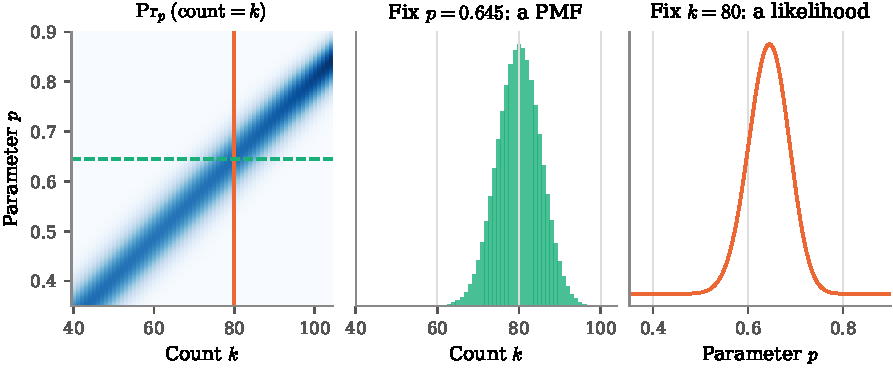
\includegraphics[width=\textwidth]{fig_likelihood_slices}
\caption{One function, two readings, for $124$ couples. Left: $\Pr_p(\text{count} = k)$ over counts $k$ (horizontal) and parameters $p$ (vertical); darker is more probable. Middle: the slice along the dashed aqua line, $p = 0.645$, a PMF over $k$ that sums to $1$. Right: the slice along the orange line, the observed $k = 80$, which is the likelihood; it peaks at $80/124 = 0.645$. The likelihood of the full sequence of $124$ turns is this curve divided by the constant $\binom{124}{80}$, which doesn't change where it peaks.}
\label{fig:likslices}
\end{figure}

\begin{pitfall}[the likelihood is not a distribution for $\theta$]
The likelihood curve in \cref{fig:likslices} looks like a density for $p$, and it isn't one.
The curve drawn there (the version for the count) has area $1/125$, not $1$, and the sequence likelihood $p^{80}(1 - p)^{44}$ has area $1.0 \times 10^{-36}$; nothing in the construction makes the area mean anything: rescale it by any constant and every comparison it supports is unchanged.
Until \cref{ch:bayes-intro}, $p$ is a fixed unknown number, not a random variable, so `the probability that $p$ is between $0.6$ and $0.7$' has no meaning here.
The likelihood is a plausibility ranking of candidate truths by how well they predicted your data.
This is why the right of \cref{fig:probstat} in \cref{ch:kiss}, which is this kind of curve for the drug data scaled to peak at $1$, has no vertical scale that could be read as a probability.
That chapter is where the parameter gets a distribution, and the likelihood is one of its two ingredients.
\end{pitfall}

\begin{worked}[the likelihoods of the two discrete families]
\begin{itemize}
\item \textbf{Bernoulli.} For $\Xton \iid \Bern(p)$, $E = \{0, 1\}$ and $\Theta = (0, 1)$. The PMF can be written in one line as $p_p(x) = p^x (1 - p)^{1 - x}$, which is $p$ at $x = 1$ and $1 - p$ at $x = 0$. Then
\[
L(x_1, \ldots, x_n; p) = \prod_{i=1}^n p^{x_i}(1 - p)^{1 - x_i} = p^{\sum_i x_i}(1 - p)^{n - \sum_i x_i}.
\]
The data enter only through the number of ones, $\sum_i x_i$.
\item \textbf{Poisson.} For $\Xton \iid \Pois(\lambda)$, $E = \{0, 1, 2, \ldots\}$ and $\Theta = (0, \infty)$:
\[
L(x_1, \ldots, x_n; \lambda) = \prod_{i=1}^n e^{-\lambda}\frac{\lambda^{x_i}}{x_i!} = e^{-n\lambda}\frac{\lambda^{\sum_i x_i}}{x_1! \cdots x_n!}.
\]
For the siblings data of \cref{ch:models}, modeled as $X_i - 1 \sim \Pois(\lambda)$, the $24$ values of $x_i - 1$ add up to $24$, and the likelihood is $e^{-24\lambda}\lambda^{24}$ divided by a constant that doesn't involve $\lambda$.
\end{itemize}
\end{worked}

Three properties of a likelihood follow straight from the product.

\begin{itemize}
\item \textbf{Order doesn't matter.} A product can be taken in any order, so the likelihood of $(1, 2, 3)$ is the likelihood of $(2, 3, 1)$. For the Bernoulli and Poisson families it depends on the data only through their sum, up to a factor that does not involve the parameter; the sum is the sufficient statistic of \cref{ch:estimators}: the likelihood never looks at anything else in the data.
\item \textbf{It updates one observation at a time.} If $L_n$ is the likelihood after $n$ observations, then $L_{n+1}(\theta) = L_n(\theta) \cdot p_\theta(x_{n+1})$. For Poisson data $1, 2$ the likelihood is $e^{-2\lambda}\lambda^3/2$; a third observation $3$ multiplies it by $e^{-\lambda}\lambda^3/6$, giving $e^{-3\lambda}\lambda^6/12$ (\cref{ex:lik-poisson-update}).
\item \textbf{It is as smooth in $\theta$ as the PMF is.} If each $p_\theta(x)$ is a continuous function of $\theta$, so is the product. A discrete model can have a perfectly smooth likelihood: the data are discrete, the parameter is not.
\end{itemize}

\section{The likelihood of a continuous model}
\label{sec:lik-continuous}

For continuous data the probability of observing exactly $x_1, \ldots, x_n$ is $0$ under every candidate, which would make every likelihood $0$ and rank nothing.
The fix is to use densities.

\begin{definition}[Likelihood, continuous model]
\label{def:likelihood-continuous}
Let $(E, (\Pr_\theta)_{\theta \in \Theta})$ be a statistical model for $\Xton$ i.i.d., where each $\Pr_\theta$ has a density $f_\theta$ \toolkit{sec:math-density}.
The \textbf{likelihood} of the model is
\begin{align*}
L_n : E^n \times \Theta &\to \real \\
(x_1, \ldots, x_n; \theta) &\mapsto \prod_{i=1}^n f_\theta(x_i).
\end{align*}
\end{definition}

\begin{inwords}
\textbf{In words.} The same recipe as for a discrete model, with each observation contributing the height of its density instead of its probability. A candidate whose density is high where your data fell scores well; one whose density is low there scores badly.
\par\smallskip
\textbf{For the kiss data.} The kiss data are discrete, so the discrete definition applies and this one doesn't. The two definitions are one idea, and from here on the chapter writes $p_\theta$ for either a PMF or a density.
\end{inwords}

\begin{intuition}[why the density is enough]
A recorded measurement is never exact.
A subway gap written down as $5$ minutes was somewhere near $5$, say within $h/2$ of it for a small $h$.
The probability of that is the area of a thin strip under the density, about $f_\lambda(5)\cdot h$.
Compare two candidate rates, and the $h$ cancels:
\[
\frac{\Pr_{\lambda_1}(\text{gap within } h/2 \text{ of } 5)}{\Pr_{\lambda_2}(\text{gap within } h/2 \text{ of } 5)} \approx \frac{f_{\lambda_1}(5)\, h}{f_{\lambda_2}(5)\, h} = \frac{f_{\lambda_1}(5)}{f_{\lambda_2}(5)}.
\]
\Cref{fig:densitystrip} shows the ratio of strip probabilities settling at the ratio of densities as the strip narrows.
Every use of a likelihood is a comparison between parameters, so the density is all it needs.
\end{intuition}

\begin{figure}[htbp]
\centering
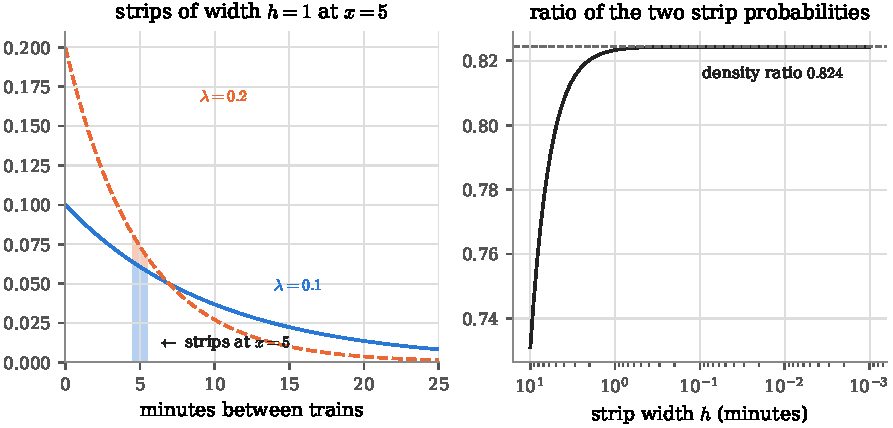
\includegraphics[width=\textwidth]{fig_density_strip}
\caption{Why a density can stand in for a probability. Left: the $\Expo(0.1)$ and $\Expo(0.2)$ densities, with the probabilities of a gap within $\frac12$ minute of $5$ shown as strips; the $\Expo(0.1)$ strip is blue, and the taller $\Expo(0.2)$ strip contains it, its extra height in orange. Right: the ratio of the two strip probabilities as the width $h$ shrinks; it settles at the ratio of the densities, $f_{0.1}(5)/f_{0.2}(5) = 0.824$.}
\label{fig:densitystrip}
\end{figure}

\begin{worked}[the likelihoods of the continuous families]
\begin{itemize}
\item \textbf{Gaussian.} For $\Xton \iid \Gauss(\mu, \sigma^2)$, $E = \real$ and $\Theta = \real \times (0, \infty)$:
\[
\begin{aligned}
L(x_1, \ldots, x_n; \mu, \sigma^2) &= \prod_{i=1}^n \frac{1}{\sigma\sqrt{2\pi}}\exp\left(-\frac{(x_i - \mu)^2}{2\sigma^2}\right)\\
&= \frac{1}{(\sigma\sqrt{2\pi})^n}\exp\left(-\frac{1}{2\sigma^2}\sum_{i=1}^n (x_i - \mu)^2\right).
\end{aligned}
\]
\item \textbf{Exponential.} For $\Xton \iid \Expo(\lambda)$, $E = (0, \infty)$ and $\Theta = (0, \infty)$. The density is $f_\lambda(x) = \lambda e^{-\lambda x}\ind(x > 0)$, so
\[
L(x_1, \ldots, x_n; \lambda) = \lambda^n e^{-\lambda \sum_i x_i} \prod_{i=1}^n \ind(x_i > 0) = \lambda^n e^{-\lambda \sum_i x_i}\, \ind\big(\min_i x_i > 0\big).
\]
The product of indicators is $1$ exactly when every $x_i$ is positive, which is when the smallest one is \toolkit{sec:math-indicator}. The indicator doesn't involve $\lambda$, and data from the model are always positive, so it is usually dropped: $L(\lambda) = \lambda^n e^{-\lambda\sum_i x_i}$.
\item \textbf{Uniform.} For $\Xton \iid \Unif([0, \theta])$, $E = [0, \infty)$ and $\Theta = (0, \infty)$. The density is $f_\theta(x) = \frac1\theta \ind(0 \leq x \leq \theta)$, so
\[
L(x_1, \ldots, x_n; \theta) = \frac{1}{\theta^n}\prod_{i=1}^n \ind(0 \leq x_i \leq \theta) = \frac{1}{\theta^n}\,\ind\big(\min_i x_i \geq 0\big)\,\ind\big(\max_i x_i \leq \theta\big).
\]
Every $x_i \leq \theta$ holds exactly when the largest does. Here the indicator involving the maximum \textit{does} depend on $\theta$, and it cannot be dropped: it is what makes this likelihood unusual (\cref{sec:lik-families}). The other indicator doesn't involve $\theta$ and is dropped as before: $L(\theta) = \theta^{-n}\ind(\theta \geq \max_i x_i)$.
\item \textbf{Mixture of two Gaussians.} For the model of \cref{sec:models-gmm}, with weight $\pi$ and components $\Gauss(\mu_1, \sigma_1^2)$ and $\Gauss(\mu_2, \sigma_2^2)$, the density of one observation is a sum, and
\[
L = \prod_{i=1}^n \left( \frac{\pi}{\sigma_1\sqrt{2\pi}} e^{-(x_i - \mu_1)^2/(2\sigma_1^2)} + \frac{1 - \pi}{\sigma_2\sqrt{2\pi}} e^{-(x_i - \mu_2)^2/(2\sigma_2^2)} \right).
\]
A product of sums does not simplify, and that is the source of the trouble in \cref{sec:lik-em}.
\end{itemize}
\end{worked}

\begin{pitfall}[an indicator you drop must not involve the parameter]
Dropping a factor from a likelihood is safe exactly when the factor doesn't depend on $\theta$: it multiplies every candidate's score by the same number and changes no comparison.
The exponential's $\ind(\min_i x_i > 0)$ is such a factor.
The uniform's $\ind(\max_i x_i \leq \theta)$ is not, and dropping it leaves $\theta^{-n}$, which grows without bound as $\theta \to 0$: the best candidate would be one under which your data were impossible.
\end{pitfall}

\section{The maximum likelihood estimator}
\label{sec:lik-mle}

\begin{definition}[Maximum likelihood estimator]
\label{def:mle}
Let $\Xton$ be an i.i.d.\ sample from a statistical model $(E, (\Pr_\theta)_{\theta \in \Theta})$ with likelihood $L$.
The \textbf{maximum likelihood estimator} (MLE) of $\theta$ is
\[
\hat{\theta}_n^{\text{MLE}} = \operatorname*{argmax}_{\theta \in \Theta} L(X_1, \ldots, X_n; \theta),
\]
provided the maximum exists and is attained at a single point.
\end{definition}

\begin{inwords}
\textbf{In words.} Among all the candidate truths the model allows, pick the one under which the data you actually got were most probable. Before the data arrive, $\hat{\theta}_n^{\text{MLE}}$ is a random variable, a function of $\Xton$ like every estimator in \cref{ch:estimators}; once they arrive it is a number, the maximum likelihood estimate.
\par\smallskip
\textbf{For the kiss data.} $L(p) = p^{80}(1 - p)^{44}$ is largest at $p = 80/124 = 0.645$ (\cref{sec:lik-families} does the calculus), so the maximum likelihood estimate is the sample proportion. In general $\hat{p}^{\text{MLE}} = \bar{R}_n$, the estimator \cref{ch:kiss} started from because it was the obvious one. In models where no estimator is obvious, the same principle still produces one.
\end{inwords}

In practice you maximize the logarithm of the likelihood, the \textbf{log-likelihood}
\[
\ell_n(\theta) = \log L(X_1, \ldots, X_n; \theta) = \sum_{i=1}^n \log p_\theta(X_i).
\]
Because $\log$ is strictly increasing, $L$ and $\ell_n$ have their maximum at the same $\theta$ \toolkit{sec:math-explog}.
There are three reasons to prefer $\ell_n$.
It turns a product of $n$ factors into a sum of $n$ terms, and sums are easier to differentiate.
It keeps the numbers in a sane range: $L(0.645) = 9.4 \times 10^{-36}$ for the kiss data, and for a few thousand observations a likelihood is smaller than any number a computer stores, while $\ell_n(0.645) = -80.65$ is an ordinary number.
And $\frac1n\ell_n(\theta)$ is an average, which is what the Law of Large Numbers and the Central Limit Theorem know how to handle; \cref{ch:mle-properties} uses that.

\Cref{fig:kissloglik} shows both curves for the kiss data.
The likelihood is a narrow peak at $0.645$ on a scale of $10^{-36}$.
The log-likelihood is a smooth hill whose top is at the same place, flat there, and $5.30$ higher than its value at $p = \frac12$.

\begin{figure}[htbp]
\centering
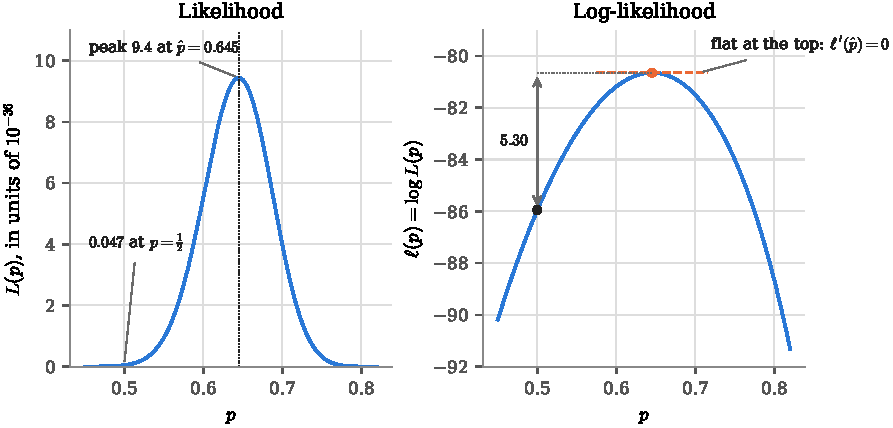
\includegraphics[width=\textwidth]{fig_kiss_loglik}
\caption{The kiss data. Left: the likelihood $L(p) = p^{80}(1 - p)^{44}$ in units of $10^{-36}$, with its peak $9.4$ at $\hat{p} = 0.645$ and the value $0.047$ at $p = \frac12$. Right: the log-likelihood $\ell(p) = 80\log p + 44\log(1 - p)$, concave, with its maximum $-80.65$ at $0.645$ where the tangent is flat, and the value $-85.95$ at $\frac12$; the gap, $5.30$, is $124$ times the KL divergence $0.0428$ of \cref{ch:distances}.}
\label{fig:kissloglik}
\end{figure}

\begin{sanitycheck}[The sharpness of the peak]
How sharply the log-likelihood curves down at its top should say something about how precisely the data pin down $p$: a flat top means many values of $p$ fit about equally well.
Check it.
For the kiss data $\ell(p) = 80\log p + 44\log(1 - p)$, so $\ell''(p) = -80/p^2 - 44/(1 - p)^2$, and at $\hat{p}$ this is $-n/(\hat{p}(1 - \hat{p})) = -541.7$.
Then $1/\sqrt{541.7} = 0.0430$, which is exactly the standard error $\sqrt{\hat{p}(1 - \hat{p})/n}$ of \cref{ch:confidence-intervals}, since $\ell''(\hat{p}) = -n/(\hat{p}(1 - \hat{p}))$.
For the subway data the same computation gives $\hat{\lambda}/\sqrt{n} = 0.020$, the standard error of \cref{ch:limit-tools}.
It is not a coincidence, and \cref{ch:mle-properties} proves it in general: the curvature of the log-likelihood at its peak estimates $n$ times the Fisher information, and one over its square root is the standard error of the MLE.
\end{sanitycheck}

\section{Finding a maximum}
\label{sec:lik-maximize}

The definition says `argmax', and an argmax has to be found.
Maximizing an arbitrary function is hard: it can have many hills, and a point where the slope is zero can be the top of a small hill, the bottom of a valley or neither.
The right of \cref{fig:concavevsnot} is $\theta \mapsto \prod_i (\theta - x_i)$ for five numbers $x_i$: four points with zero slope, and on the whole line no maximum at all.
The functions that are easy to maximize are the concave ones.

\begin{definition}[Concave and convex functions]
\label{def:concave}
A twice-differentiable function $h: \Theta \to \real$ on an interval $\Theta \subset \real$ is \textbf{concave} if $h''(\theta) \leq 0$ for every $\theta \in \Theta$, and \textbf{strictly concave} if $h''(\theta) < 0$ for every $\theta$.
(The `strictly' version here is stronger than the usual chord definition, which also allows $h'' = 0$ at isolated points, as for $-\theta^4$; it is the version this book uses.)
It is (strictly) \textbf{convex} if $-h$ is (strictly) concave, that is, $h'' \geq 0$ ($h'' > 0$).
\end{definition}

\begin{inwords}
\textbf{In words.} A concave function's slope never increases: it is a hill, or a straight line, never a valley. Every chord lies below the graph \toolkit{sec:math-convex}. On their natural domains, $-\theta^2$, $\sqrt{\theta}$, $\log\theta$ and $\sin\theta$ on $[0, \pi]$ are concave; $2\theta - 3$ is both concave and convex; $\theta^2$ and $e^\theta$ are convex.
\par\smallskip
\textbf{For the kiss data.} $\ell''(p) = -80/p^2 - 44/(1 - p)^2$ is negative for every $p \in (0, 1)$, so the kiss log-likelihood is strictly concave: one hill, no valleys, as the right of \cref{fig:kissloglik} shows.
\end{inwords}

\begin{proposition}[Maximizing a strictly concave function]
\label{prop:concave-max}
Let $h$ be strictly concave and differentiable on an open interval $\Theta$.
If $h'(\hat{\theta}) = 0$ at some $\hat{\theta} \in \Theta$, then $\hat{\theta}$ is the unique maximizer of $h$ on $\Theta$.
If $h'$ never vanishes, $h$ has no maximum on $\Theta$.
\end{proposition}

\optionalproof{Strict concavity makes the slope strictly decreasing, so it can cross zero at most once, and on each side of the crossing the function moves away from the top.}
\begin{proof}
Since $h'' < 0$, $h'$ is strictly decreasing.
If $h'(\hat{\theta}) = 0$, then $h' > 0$ to the left of $\hat{\theta}$ and $h' < 0$ to the right: $h$ increases up to $\hat{\theta}$ and decreases after, so $h(\theta) < h(\hat{\theta})$ for every $\theta \neq \hat{\theta}$.
At an interior maximizer the derivative must be $0$, since otherwise moving a little in the direction of the slope would increase $h$; so if $h'$ never vanishes there is no interior maximizer, and on an open interval there is no other kind.
\end{proof}

\begin{figure}[htbp]
\centering
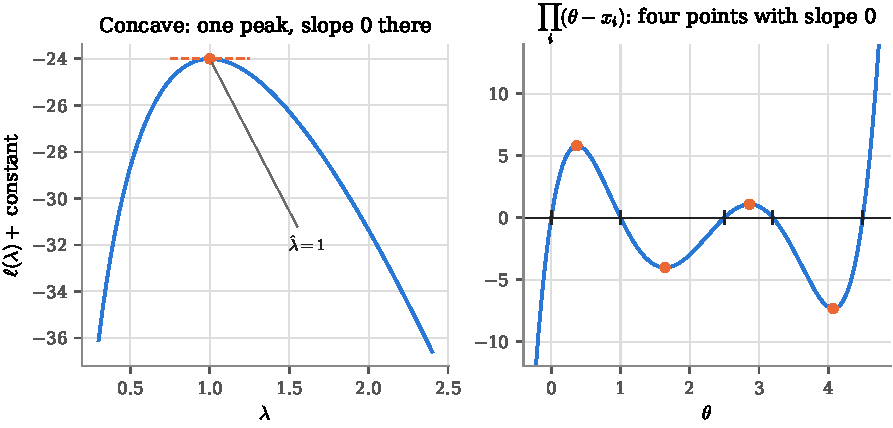
\includegraphics[width=\textwidth]{fig_concave_vs_not}
\caption{Easy and hard functions to maximize. Left: the Poisson log-likelihood of the siblings data, $-24\lambda + 24\log\lambda$ up to a constant, strictly concave with its single maximum at $\hat{\lambda} = 1$, where the slope is $0$. Right: $\prod_i (\theta - x_i)$ for the five values marked on the axis; four points have slope $0$ (dots), and setting the derivative to $0$ finds all four without saying which, if any, is a maximum.}
\label{fig:concavevsnot}
\end{figure}

So the recipe for a one-parameter model is: write $\ell_n$, check that it is strictly concave, solve $\ell_n'(\theta) = 0$.
The Bernoulli, Poisson and exponential log-likelihoods of \cref{sec:lik-families} pass the check; the Gaussian needs a two-step argument instead; the uniform fails it entirely.

For a parameter with several coordinates, $\theta = (\theta_1, \ldots, \theta_d)$, the derivative becomes the \textbf{gradient} $\nabla\ell_n(\theta)$, the vector of partial derivatives, and the second derivative becomes the \textbf{Hessian} $\nabla^2\ell_n(\theta)$, the $d \times d$ matrix of second partial derivatives \toolkit{sec:math-multivar}.
The first-order condition is $\nabla\ell_n(\hat{\theta}) = 0$, a system of $d$ equations.
A sufficient condition for strict concavity (on a $\Theta$ that contains the segment between any two of its points) is a negative definite Hessian at every $\theta$, which for $d = 2$ means its top-left entry is negative and its determinant positive.
Under it, the solution of $\nabla\ell_n = 0$, if there is one, is the unique maximizer, as in one dimension.
When there is no formula for the solution, numerical methods find it; for a concave $\ell_n$ they are reliable, and the subject of convex optimization is how to do it fast.

\section{Maximum likelihood estimators of the standard families}
\label{sec:lik-families}

\begin{worked}[Bernoulli: the kiss data]
For $\Xton \iid \Bern(p)$ with $S = \sum_i X_i$ ones,
\[
\ell_n(p) = S\log p + (n - S)\log(1 - p), \quad \ell_n'(p) = \frac{S}{p} - \frac{n - S}{1 - p}, \quad \ell_n''(p) = -\frac{S}{p^2} - \frac{n - S}{(1 - p)^2} < 0.
\]
Setting $\ell_n'(p) = 0$ gives $S(1 - p) = (n - S)p$, so $p = S/n$:
\[
\hat{p}^{\text{MLE}} = \bar{X}_n.
\]
(If $S = 0$ or $S = n$ there is no solution in $(0, 1)$; \cref{sec:lik-fail} deals with that.)
For the kiss data, $\hat{p} = 80/124 = 0.645$, the estimate of every earlier chapter.
\end{worked}

\begin{worked}[Poisson: the siblings data]
For $\Xton \iid \Pois(\lambda)$,
\[
\ell_n(\lambda) = -n\lambda + \Big(\sum_i X_i\Big)\log\lambda - \sum_i \log(X_i!), \quad \ell_n'(\lambda) = -n + \frac{\sum_i X_i}{\lambda}, \quad \ell_n''(\lambda) = -\frac{\sum_i X_i}{\lambda^2} < 0
\]
(when at least one $X_i$ is positive).
The first-order condition gives
\[
\hat{\lambda}^{\text{MLE}} = \bar{X}_n.
\]
For the siblings data, with $X_i - 1 \sim \Pois(\lambda)$, the sample mean of the $x_i - 1$ is $24/24 = 1$, so $\hat{\lambda} = 1.0$: the fit drawn in \cref{fig:siblings}, and the left of \cref{fig:concavevsnot}.
\end{worked}

\begin{worked}[exponential: the subway data]
For $\Xton \iid \Expo(\lambda)$,
\[
\ell_n(\lambda) = n\log\lambda - \lambda\sum_i X_i, \quad \ell_n'(\lambda) = \frac{n}{\lambda} - \sum_i X_i, \quad \ell_n''(\lambda) = -\frac{n}{\lambda^2} < 0,
\]
and
\[
\hat{\lambda}^{\text{MLE}} = \frac{n}{\sum_i X_i} = \frac{1}{\bar{X}_n}.
\]
For the $64$ subway gaps averaging $6.23$ minutes, $\hat{\lambda} = 0.1605$ per minute, the estimator of \cref{ch:limit-tools}.
\Cref{ch:estimators} showed it is biased upward, $\E[1/\bar{T}_n] = \frac{n}{n-1}\lambda$: a maximum likelihood estimator need not be unbiased.
\end{worked}

\begin{worked}[Gaussian: the boarding data]
For $\Xton \iid \Gauss(\mu, \sigma^2)$ the parameter has two coordinates, and
\[
\ell_n(\mu, \sigma^2) = -\frac{n}{2}\log(2\pi\sigma^2) - \frac{1}{2\sigma^2}\sum_{i=1}^n (X_i - \mu)^2.
\]
Maximize in $\mu$ first, for a fixed $\sigma^2$.
The only term involving $\mu$ is $-\frac{1}{2\sigma^2}\sum_i(X_i - \mu)^2$, and the split
\[
\sum_{i=1}^n (X_i - \mu)^2 = \sum_{i=1}^n (X_i - \bar{X}_n)^2 + n(\bar{X}_n - \mu)^2
\]
(write $X_i - \mu = (X_i - \bar{X}_n) + (\bar{X}_n - \mu)$, square, and note the cross terms add to $0$) shows it is largest at $\mu = \bar{X}_n$, whatever $\sigma^2$ is.
Now put $\mu = \bar{X}_n$ and maximize in $\sigma^2$.
With $D = \sum_i (X_i - \bar{X}_n)^2$, the function $-\frac{n}{2}\log\sigma^2 - D/(2\sigma^2)$ has derivative $-\frac{n}{2\sigma^2} + \frac{D}{2\sigma^4}$, positive for $\sigma^2 < D/n$ and negative after.
Chaining the two steps, for every $(\mu, \sigma^2)$,
\[
\ell_n(\mu, \sigma^2) \leq \ell_n(\bar{X}_n, \sigma^2) \leq \ell_n(\bar{X}_n, D/n),
\]
with equality only at $(\bar{X}_n, D/n)$, so
\[
\hat{\mu}^{\text{MLE}} = \bar{X}_n, \qquad \widehat{\sigma^2}^{\text{MLE}} = \frac1n\sum_{i=1}^n (X_i - \bar{X}_n)^2.
\]
At the maximum the gradient is $0$ and the Hessian is the diagonal matrix with entries $-n/\widehat{\sigma^2}$ and $-n/(2\widehat{\sigma^2}^2)$, negative definite.
(The log-likelihood is not concave in $\sigma^2$ everywhere, which is why the argument went one coordinate at a time instead of checking the Hessian at every point. It also needs $D > 0$: if every observation is the same number, the likelihood grows without bound as $\sigma^2 \to 0$.)

For the $72$ flights boarded rear to front, with mean $24.2$ minutes and standard deviation $s = 2.1$ (taken to be computed with $n - 1$, the usual convention), $\hat{\mu} = 24.2$ and $\widehat{\sigma^2} = \frac{71}{72} \times 2.1^2 = 4.35$.
\Cref{fig:gaussloglik} draws the log-likelihood surface.
\end{worked}

\begin{figure}[htbp]
\centering
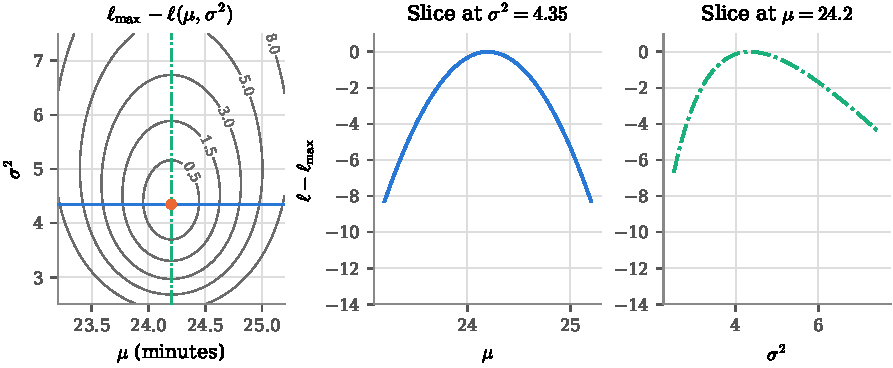
\includegraphics[width=\textwidth]{fig_gauss_loglik}
\caption{The Gaussian log-likelihood of the boarding data ($n = 72$, mean $24.2$, standard deviation $2.1$), measured from its maximum. Left: contours over $(\mu, \sigma^2)$, labeled by how far each lies below the maximum, with the maximum at $(24.2, 4.35)$ and the two slices drawn as lines (blue solid, aqua dash-dot). Middle: the slice at $\sigma^2 = 4.35$, symmetric in $\mu$. Right: the slice at $\mu = 24.2$, lopsided: variances above the maximum are penalized less than variances below it.}
\label{fig:gaussloglik}
\end{figure}

\begin{bridge}[$n$ or $n - 1$?]
The maximum likelihood estimator of the variance divides by $n$.
The sample variance you were taught divides by $n - 1$.
They differ by the factor $(n - 1)/n$, which is $0.986$ for the boarding data: $4.35$ against $4.41$.
\Cref{ch:estimators} showed that dividing by $n$ is biased low by exactly that factor and that dividing by $n - 1$ removes the bias; it also showed that removing the bias is not the same as minimizing the risk.
Maximum likelihood doesn't aim at unbiasedness, so it lands on $n$.
For large $n$ the difference is negligible, and every large-sample result in \cref{ch:mle-properties} holds for either.
\end{bridge}

\begin{bridge}[least squares is maximum likelihood]
The Gaussian log-likelihood contains $-\frac{1}{2\sigma^2}\sum_i (X_i - \mu)^2$, so maximizing it over $\mu$ is minimizing a sum of squared deviations.
The same is true when $\mu$ is replaced by a regression line $a + b x_i$: if the errors around the line are Gaussian with a common variance, the maximum likelihood estimates of $a$ and $b$ are the least squares estimates of an introductory regression course.
\Cref{ch:regression-uni} starts from that observation.
\end{bridge}

\begin{worked}[uniform: where calculus fails]
For $\Xton \iid \Unif([0, \theta])$ the likelihood is $L(\theta) = \theta^{-n}\ind(\theta \geq \max_i X_i)$.
Below the largest observation the likelihood is $0$ (a $\theta$ smaller than an observation makes that observation impossible). From the largest observation on it is $\theta^{-n}$, which decreases, with derivative $-n\theta^{-n-1}$, never $0$.
The maximum is at the jump:
\[
\hat{\theta}^{\text{MLE}} = \max_i X_i.
\]
\Cref{fig:uniformlik} draws it for five observations whose largest is $7.6$.
Setting the derivative to $0$ would have found only the flat stretch below $\max_i X_i$, where the likelihood is $0$; the recipe of \cref{sec:lik-maximize} assumes a smooth function with its maximum inside $\Theta$, and this likelihood is neither smooth at its maximum nor concave.
The estimator is also biased: the largest of $n$ draws always falls short of $\theta$, and $\E[\max_i X_i] = \frac{n}{n+1}\theta$ (\cref{ex:lik-uniform}). Multiplying by $\frac{n+1}{n}$ removes the bias.
\end{worked}

\begin{figure}[htbp]
\centering
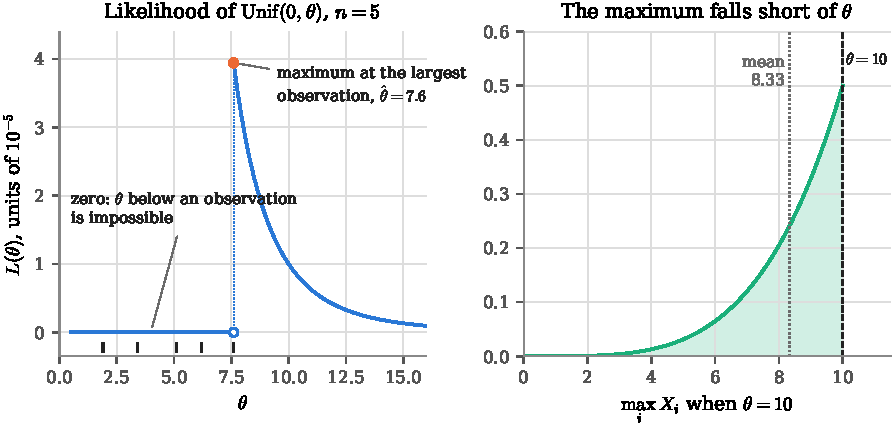
\includegraphics[width=\textwidth]{fig_uniform_likelihood}
\caption{Left: the likelihood of $\Unif([0, \theta])$ for five observations (ticks below the axis), zero until the largest observation, $7.6$, then $\theta^{-5}$, decreasing. The maximum is at the jump, where no derivative is zero. Right: the density $5m^4/10^5$ of the maximum of five draws when $\theta = 10$; it never exceeds $10$, and its mean is $8.33$.}
\label{fig:uniformlik}
\end{figure}

\begin{intuition}[the German tank problem]
The uniform model once estimated an enemy's tank production.
During the Second World War, Allied statisticians estimated German tank production from the serial numbers on captured tanks.
If serial numbers run $1, 2, \ldots, N$ and the captured ones are a random sample, $N$ plays the role of $\theta$, the largest serial number seen is the maximum likelihood estimate, and correcting it for the shortfall of the maximum gives a better one.
Their serial-number estimates, which refined this idea and used markings on several components (chassis, gearboxes, wheels), for three months, beside the figures from conventional intelligence and the German records found after the war:\footnote{R.~Ruggles and H.~Brodie, `An empirical approach to economic intelligence in World War II', \textit{Journal of the American Statistical Association} 42 (1947), 72--91.}
\begin{center}
\begin{tabular}{lrrr}
Month & Statistical estimate & Intelligence estimate & German records \\
\hline
June 1940 & 169 & 1{,}000 & 122 \\
June 1941 & 244 & 1{,}550 & 271 \\
August 1942 & 327 & 1{,}550 & 342
\end{tabular}
\end{center}
The model is crude (serial numbers are not quite a random sample), and its estimates were within $50$ tanks of the records while the intelligence estimates were off by a factor of about four to eight.
\end{intuition}

One more property makes maximum likelihood convenient: it doesn't care how the parameter is written.

\begin{proposition}[Invariance]
\label{prop:mle-invariance}
Let $g: \Theta \to g(\Theta)$ be one-to-one, and reparameterize the model by $\eta = g(\theta)$.
If $\hat{\theta}$ is the MLE of $\theta$, then $g(\hat{\theta})$ is the MLE of $\eta$.
\end{proposition}

\optionalproof{Reparameterizing relabels the candidates without changing any candidate's likelihood, so the winner is the same distribution under its new label.}
\begin{proof}
The candidate labeled $\eta$ in the new parameterization is the distribution $\Pr_{g^{-1}(\eta)}$, so its likelihood is $L(g^{-1}(\eta))$.
This is largest when $g^{-1}(\eta) = \hat{\theta}$, that is, at $\eta = g(\hat{\theta})$.
\end{proof}

For the subway data, the mean gap $\beta = 1/\lambda$ has MLE $1/\hat{\lambda} = \bar{X}_n = 6.23$ minutes.
For the boarding data, the standard deviation has MLE $\sqrt{4.35} = 2.09$ minutes.
Invariance does not carry unbiasedness along: $\bar{X}_n$ is unbiased for $\beta$ and $1/\bar{X}_n$ is biased for $\lambda$, though both are maximum likelihood estimators.

\section{When the maximum likelihood estimator fails to exist or isn't unique}
\label{sec:lik-fail}

\Cref{def:mle} said `provided the maximum exists and is attained at a single point'. Both can fail, in ordinary models.

\begin{pitfall}[three ways the definition can fail]
\begin{itemize}
\item \textbf{No maximum: the data sit on the boundary.} If every observation in a Bernoulli sample is $0$ ($S = 0$), then $L(p) = (1 - p)^n$ increases as $p$ decreases and has no maximum on $\Theta = (0, 1)$: the supremum is at $p = 0$, which the model excludes. For the kiss data this can't happen in practice (under $p = 0.645$ its probability is $0.355^{124}$), but for $n = 5$ observations of an outcome with $p = 0.1$ it happens $59\%$ of the time. The usual repair is to allow $p \in [0, 1]$, and then $\hat{p} = 0$.
\item \textbf{More than one maximum.} For $\Xton \iid \Unif([\theta, \theta + 1])$, $L(\theta) = \ind(\theta \leq \min_i X_i)\,\ind(\theta + 1 \geq \max_i X_i)$, which equals $1$ on the whole interval $[\max_i X_i - 1, \min_i X_i]$ and $0$ elsewhere. Every point of that interval is a maximizer (\cref{ex:lik-unif-shift}).
\item \textbf{An unbounded likelihood.} In the mixture of two Gaussians with unknown variances, put $\mu_1 = x_1$ and let $\sigma_1 \to 0$. The first factor of the likelihood contains $\pi/(\sigma_1\sqrt{2\pi})$, which goes to infinity, while every other factor stays above $(1 - \pi)$ times the second component's density at its point, which is positive. The likelihood is unbounded: a component of zero width sitting on one data point `explains' that point infinitely well. The maximum likelihood estimator of a mixture with free variances does not exist, and what is computed in practice is the best local maximum away from these spikes.
\end{itemize}
\end{pitfall}

\section{No formula: mixtures and the EM algorithm}
\label{sec:lik-em}

The left of \cref{fig:emfaithful} is a histogram of the $272$ waiting times, in minutes, between eruptions of the Old Faithful geyser in Yellowstone National Park.\footnote{The version of the data distributed with W.~H\"ardle, \textit{Smoothing Techniques} (Springer, 1991); A.~Azzalini and A.~W.~Bowman, `A look at some data on the Old Faithful geyser', \textit{Applied Statistics} 39 (1990), 357--365, analyze a longer record.}
It has two humps, one near $55$ minutes and one near $80$, and a single Gaussian (orange) fits it badly.
A mixture of two Gaussians is the natural model: each wait comes from a short-wait regime or a long-wait regime, and you don't get to see which.

The log-likelihood of the mixture,
\[
\ell_n = \sum_{i=1}^n \log\Big( \pi\, f_{\mu_1, \sigma_1^2}(X_i) + (1 - \pi)\, f_{\mu_2, \sigma_2^2}(X_i) \Big),
\]
has the log of a sum in every term, and setting its gradient to $0$ gives five equations with no closed-form solution.
The \textbf{EM algorithm} (expectation-maximization, given its general form and its name in 1977 and still in everyday use) gets around this with one idea: pretend you know which regime each observation came from.

\subsection*{The complete data}

Recall the generative story of \cref{sec:models-gmm}: draw $Z_i \sim \Bern(\pi)$; if $Z_i = 1$, draw $X_i$ from component $1$, otherwise from component $2$.
If you observed the labels $Z_i$ along with the $X_i$, the log-likelihood of the \textit{complete data} $(X_i, Z_i)$ would split:
\[
\ell_n^{\text{comp}} = \sum_{i=1}^n \Big[ Z_i\big(\log\pi + \log f_{\mu_1, \sigma_1^2}(X_i)\big) + (1 - Z_i)\big(\log(1 - \pi) + \log f_{\mu_2, \sigma_2^2}(X_i)\big) \Big].
\]
There is no log of a sum: each observation contributes to exactly one component.
Maximizing it is two separate Gaussian fits and one Bernoulli fit, each done in \cref{sec:lik-families}: $\hat{\pi}$ is the share of observations labeled $1$, and $\hat{\mu}_1$, $\hat{\sigma}_1^2$ are the mean and divide-by-$n$ variance of the observations labeled $1$ (and likewise for component $2$).

\subsection*{The E step: guess the labels}

You don't observe the $Z_i$.
The best guess for $Z_i$ given $X_i$, under the current parameter values, is its conditional expectation, which is the probability that $X_i$ came from component $1$.
By Bayes' formula,
\[
w_i = \E[Z_i \mid X_i] = \Pr(Z_i = 1 \mid X_i) = \frac{\pi\, f_{\mu_1, \sigma_1^2}(X_i)}{\pi\, f_{\mu_1, \sigma_1^2}(X_i) + (1 - \pi)\, f_{\mu_2, \sigma_2^2}(X_i)} \in (0, 1).
\]
A wait of $50$ minutes gets $w_i$ close to $1$; a wait of $85$ gets $w_i$ close to $0$; a wait of $67$, between the humps, gets something in the middle.
Guessing $Z_i \approx \E[Z_i] = \pi$, the same for every observation, would ignore the data entirely; conditioning on $X_i$ is what makes the guess useful.

\subsection*{The M step: fit as if the guesses were labels}

Replace each $Z_i$ in $\ell_n^{\text{comp}}$ by $w_i$ and maximize.
This is legitimate because $\ell_n^{\text{comp}}$ is linear in each $Z_i$, so its expectation given the data, under the current parameter values, is $\ell_n^{\text{comp}}$ with each $Z_i$ replaced by $w_i$.
The same calculus as before, with weights, gives
\[
\hat{\pi} = \frac1n\sum_i w_i, \quad \hat{\mu}_1 = \frac{\sum_i w_i X_i}{\sum_i w_i}, \quad \hat{\sigma}_1^2 = \frac{\sum_i w_i (X_i - \hat{\mu}_1)^2}{\sum_i w_i},
\]
and the same for component $2$ with weights $1 - w_i$ (\cref{ex:lik-em-mstep}).
Each observation is split between the components in proportion to how likely it is to belong to each.

\begin{worked}[the EM algorithm]
\begin{enumerate}[nosep]
\item Start from some values of $\pi, \mu_1, \mu_2, \sigma_1^2, \sigma_2^2$.
\item \textbf{E step:} compute $w_i$ for every observation from the current values.
\item \textbf{M step:} update all five parameters by the weighted formulas.
\item Repeat steps 2 and 3 until the parameters stop changing.
\end{enumerate}
For Old Faithful, starting from means $50$ and $70$, both standard deviations $10$ and $\pi = \frac12$, the algorithm settles on weight $0.36$ for $\Gauss(54.6, 5.87^2)$ and $0.64$ for $\Gauss(80.1, 5.87^2)$: about a third of the waits are short, averaging $55$ minutes, and the rest are long, averaging $80$. The fitted mixture is the blue curve in \cref{fig:emfaithful}. Its log-likelihood is $-1034.0$, against $-1095.3$ for the best single Gaussian.
\end{worked}

\begin{figure}[htbp]
\centering
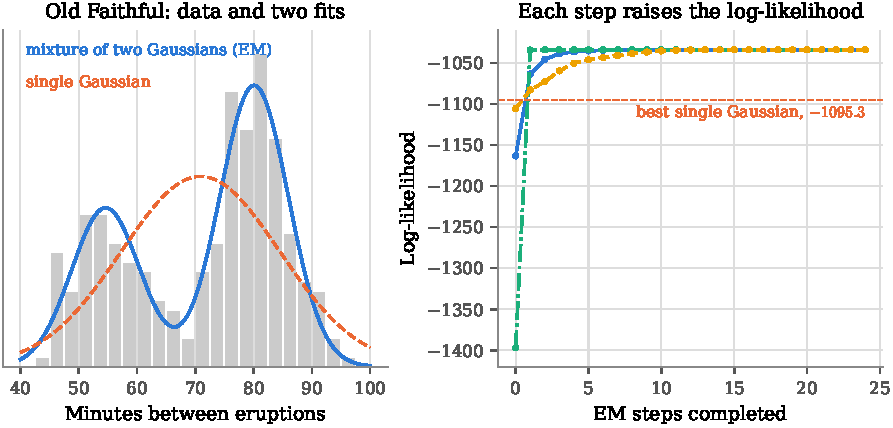
\includegraphics[width=\textwidth]{fig_em_faithful}
\caption{The EM algorithm on the $272$ waiting times between eruptions of Old Faithful. Left: the histogram, the best single Gaussian (orange, dashed) and the two-component mixture fitted by EM (blue): weight $0.36$ on $\Gauss(54.6, 5.87^2)$ and $0.64$ on $\Gauss(80.1, 5.87^2)$. Right: the log-likelihood at the start and after each EM step, from three starting points: means $50$ and $70$ (blue, solid), $40$ and $95$ (aqua, dash-dot), $65$ and $75$ (yellow, dashed). It never decreases, and all three runs reach $-1034.0$, well above the single Gaussian's $-1095.3$ (orange line).}
\label{fig:emfaithful}
\end{figure}

The right of \cref{fig:emfaithful} shows the property that makes EM trustworthy as far as it goes: every step raises the log-likelihood or leaves it unchanged.
That fact is proved in \cref{sec:proof-em} of \cref{app:proofs}, with an argument that uses the nonnegativity of the KL divergence; nothing later in the book depends on it.
What it does not guarantee is that EM reaches the highest point.
It climbs whatever hill it starts near, which may be a local maximum or one of the spikes of \cref{sec:lik-fail}.
In practice EM is run from several starting points and the run with the largest log-likelihood is kept.
EM is guaranteed to climb, not to reach the top: the results that guarantee it reaches the maximum likelihood estimate assume a starting point close enough to it, or well-separated components.

\begin{pitfall}[which component is which]
EM's labels `component $1$' and `component $2$' mean nothing.
Start it with the means the other way round and it returns the same fit with the labels swapped: weight $0.64$ on $\Gauss(80.1, 5.87^2)$ and $0.36$ on $\Gauss(54.6, 5.87^2)$.
Both have the same likelihood, since they are the same distribution.
This is the label switching of \cref{sec:models-gmm}: the mixture's parameter is identifiable only up to relabeling, so every peak of its likelihood has a twin with the labels swapped.
\end{pitfall}

\section{What comes next}
\label{sec:lik-next}

This chapter defined the maximum likelihood estimator and computed it.
\Cref{ch:mle-properties} asks how good it is, and answers with three results that hold for every well-behaved model at once.
It is consistent, by the argument \cref{fig:klestimate} drew: the average log-likelihood converges to a function maximized at the truth.
It is asymptotically normal, by the Central Limit Theorem applied to the derivative of the log-likelihood.
And its asymptotic variance is one over the Fisher information, the curvature that the sanity check of \cref{sec:lik-mle} found matching the standard errors of earlier chapters.
\Cref{ch:mom-mestimation} generalizes in two directions: the method of moments, an older and simpler recipe that often gives the same answer, and M-estimation, which maximizes or minimizes averages other than the log-likelihood.

\section{Summary}
\label{sec:lik-summary}

\begin{itemize}[nosep]
\item The likelihood $L(\theta) = \prod_i p_\theta(x_i)$ (PMFs) or $\prod_i f_\theta(x_i)$ (densities) is the probability or density of the observed data under each candidate $\theta$: the joint PMF read with the data fixed and the parameter varying. It is not a distribution for $\theta$; only ratios of likelihoods mean something. Kiss data: $L(p) = p^{80}(1 - p)^{44}$, $200$ times larger at $0.645$ than at $\frac12$.
\item A density works in place of a probability because a recorded value stands for a small interval, whose width cancels in every comparison between parameters.
\item The likelihood ignores the order of the data, updates one observation at a time, and is as smooth in $\theta$ as the PMF or density. Factors that don't involve $\theta$ (the exponential's indicator) can be dropped; factors that do (the uniform's $\ind(\theta \geq \max_i x_i)$) cannot.
\item MLE: $\hat{\theta}^{\text{MLE}} = \operatorname{argmax}_\theta L = \operatorname{argmax}_\theta \ell_n$, with $\ell_n = \sum_i \log p_\theta(X_i)$. If $\ell_n$ is strictly concave, the solution of $\ell_n' = 0$ (or $\nabla\ell_n = 0$) is the unique maximizer; in several dimensions, a negative definite Hessian everywhere is enough for strict concavity.
\item Bernoulli $\bar{X}_n$ ($0.645$ for the kiss data); Poisson $\bar{X}_n$ ($1.0$ for the siblings); exponential $1/\bar{X}_n$ ($0.1605$ per minute for the subway); Gaussian $\bar{X}_n$ and $\frac1n\sum(X_i - \bar{X}_n)^2$ ($24.2$ and $4.35$ for boarding); uniform $\max_i X_i$, found at a jump rather than where a derivative vanishes, and biased low by the factor $n/(n+1)$.
\item The curvature of the log-likelihood at its peak gives the standard error: $1/\sqrt{541.7} = 0.043$ for the kiss data.
\item Invariance: the MLE of $g(\theta)$ is $g(\hat{\theta})$ for one-to-one $g$. Unbiasedness is not invariant.
\item The MLE can fail to exist (all-zero Bernoulli data on $(0, 1)$; mixtures with free variances, whose likelihood is unbounded) or be non-unique ($\Unif([\theta, \theta+1])$).
\item EM for mixtures: E step $w_i = \Pr(Z_i = 1 \mid X_i)$ by Bayes' formula; M step, weighted proportions, means and variances. No step lowers the log-likelihood; it can stop at a local maximum, so run it from several starts. Old Faithful: weight $0.36$ on mean $54.6$, $0.64$ on mean $80.1$, log-likelihood $-1034.0$ against $-1095.3$ for one Gaussian.
\end{itemize}

\section{Exercises}
\label{sec:lik-exercises}

\begin{exercise}
\label{ex:lik-poisson-update}
Let $\Xton \iid \Pois(\lambda)$. You observe $X_1 = 1$, $X_2 = 2$. Compute $L_2(1, 2; \lambda)$. A third observation $X_3 = 3$ arrives: compute $L_3(1, 2, 3; \lambda)$ in two ways, from the definition and by updating $L_2$. Then compute $L_3(2, 3, 1; \lambda)$ and explain why it is the same.
\end{exercise}
\begin{solution}
$L_2(1, 2; \lambda) = e^{-\lambda}\frac{\lambda^1}{1!} \cdot e^{-\lambda}\frac{\lambda^2}{2!} = e^{-2\lambda}\frac{\lambda^3}{2}$. From the definition, $L_3(1, 2, 3; \lambda) = e^{-3\lambda}\frac{\lambda^{1+2+3}}{1!\,2!\,3!} = e^{-3\lambda}\frac{\lambda^6}{12}$. By updating, $L_3 = L_2 \cdot e^{-\lambda}\frac{\lambda^3}{3!} = e^{-2\lambda}\frac{\lambda^3}{2}\cdot e^{-\lambda}\frac{\lambda^3}{6} = e^{-3\lambda}\frac{\lambda^6}{12}$. $L_3(2, 3, 1; \lambda)$ is the same product with the factors in a different order, so it is also $e^{-3\lambda}\lambda^6/12$: the likelihood of i.i.d.\ data does not depend on the order of the observations. The MLE from the three observations is $\bar{X}_3 = 2$.
\end{solution}

\begin{exercise}
\label{ex:lik-continuity}
Let $(\mathbb{Z}, (\Pr_\theta)_{\theta \in \real})$ be a discrete model whose PMF $p_\theta(x)$ is a continuous function of $\theta$ for each fixed $x$. True or false: for fixed data $x_1, \ldots, x_n$, the likelihood $\theta \mapsto L_n(x_1, \ldots, x_n; \theta)$ is continuous. Give a discrete model with a smooth likelihood.
\end{exercise}
\begin{solution}
True. $L_n(\theta) = \prod_{i=1}^n p_\theta(x_i)$ is a product of $n$ continuous functions of $\theta$, and a product of continuous functions is continuous. The Bernoulli likelihood $p^{S}(1 - p)^{n - S}$ is a polynomial in $p$, as smooth as a function can be, although the data take only the values $0$ and $1$. The Poisson likelihood $e^{-n\lambda}\lambda^{\sum x_i}/\prod x_i!$ is another.
\end{solution}

\begin{exercise}
\label{ex:lik-gauss-known-mean}
Let $\Xton \iid \Gauss(0, \sigma^2)$ with $\sigma^2 > 0$ unknown. Find the MLE of $\sigma^2$, check that the log-likelihood has a unique maximum, and use invariance to find the MLE of $\sigma$.
\end{exercise}
\begin{solution}
$\ell_n(\sigma^2) = -\frac{n}{2}\log(2\pi\sigma^2) - \frac{1}{2\sigma^2}\sum_i X_i^2$. With $v = \sigma^2$ and $Q = \sum_i X_i^2$, $\ell_n'(v) = -\frac{n}{2v} + \frac{Q}{2v^2} = \frac{Q - nv}{2v^2}$, positive for $v < Q/n$ and negative for $v > Q/n$, so the unique maximizer is $\widehat{\sigma^2} = \frac1n\sum_i X_i^2$. (The log-likelihood is not concave in $v$ for all $v$, which is why the sign of the derivative is used instead of the second derivative.) It is unbiased here, since the mean is known: $\E[X_i^2] = \sigma^2$. By invariance, $\hat{\sigma} = \sqrt{\frac1n\sum_i X_i^2}$.
\end{solution}

\begin{exercise}
\label{ex:lik-uniform}
Let $\Xton \iid \Unif([0, \theta])$ and $M = \max_i X_i$. Show that $\Pr(M \leq m) = (m/\theta)^n$ for $0 \leq m \leq \theta$, find the density of $M$, and show that $\E[M] = \frac{n}{n+1}\theta$. Which multiple of $M$ is unbiased?
\end{exercise}
\begin{solution}
$M \leq m$ exactly when every $X_i \leq m$, and by independence $\Pr(M \leq m) = \prod_i \Pr(X_i \leq m) = (m/\theta)^n$. Differentiating, $M$ has density $n m^{n-1}/\theta^n$ on $[0, \theta]$. Then $\E[M] = \int_0^\theta m \cdot \frac{n m^{n-1}}{\theta^n}\, \mathrm{d}m = \frac{n}{\theta^n}\cdot\frac{\theta^{n+1}}{n+1} = \frac{n}{n+1}\theta$. So $\frac{n+1}{n}M$ is unbiased. For the five observations of \cref{fig:uniformlik}, $\frac65 \times 7.6 = 9.12$. The bias of $M$ is $-\theta/(n+1)$, of order $1/n$, and its standard deviation is also of order $1/n$, not $1/\sqrt{n}$: this model is not one of the regular models whose large-sample theory \cref{ch:mle-properties} develops.
\end{solution}

\begin{exercise}
\label{ex:lik-unif-shift}
Let $\Xton \iid \Unif([\theta, \theta + 1])$ with $\theta \in \real$. Write the likelihood and show that every $\theta$ in $[\max_i X_i - 1, \min_i X_i]$ maximizes it. Why is that interval never empty?
\end{exercise}
\begin{solution}
Each density is $\ind(\theta \leq x_i \leq \theta + 1)$, so $L(\theta) = \prod_i \ind(\theta \leq x_i)\ind(x_i \leq \theta + 1) = \ind(\theta \leq \min_i x_i)\,\ind(\theta \geq \max_i x_i - 1)$. It is $1$ on $[\max_i x_i - 1, \min_i x_i]$ and $0$ elsewhere, so every point of that interval maximizes it and the MLE is not unique. The interval is nonempty because all the data lie in an interval of length $1$, $[\theta^*, \theta^* + 1]$, so $\max_i x_i - \min_i x_i \leq 1$. Its midpoint is a sensible choice of estimate, but the likelihood alone doesn't pick it.
\end{solution}

\begin{exercise}
\label{ex:lik-geometric}
A basketball player takes shots until the first one goes in; the number of shots is $X \sim \text{Geom}(p)$, with $\Pr(X = k) = (1 - p)^{k-1}p$ for $k = 1, 2, \ldots$. Over $n$ independent rounds the numbers of shots are $\Xton$. Find the MLE of $p$, and evaluate it for rounds of $3$, $1$, $2$, $5$ and $1$ shots.
\end{exercise}
\begin{solution}
$\ell_n(p) = \sum_i\big[(X_i - 1)\log(1 - p) + \log p\big] = (S - n)\log(1 - p) + n\log p$ with $S = \sum_i X_i$. $\ell_n'(p) = -\frac{S - n}{1 - p} + \frac{n}{p} = 0$ gives $n(1 - p) = (S - n)p$, so $p = n/S$: $\hat{p} = 1/\bar{X}_n$. $\ell_n''(p) = -\frac{S - n}{(1-p)^2} - \frac{n}{p^2} < 0$, so this is the unique maximum. For the data, $S = 12$ and $n = 5$, so $\hat{p} = 5/12 = 0.417$: five makes in twelve shots.
\end{solution}

\begin{exercise}
\label{ex:lik-shifted-expo}
Let $\Xton$ be i.i.d.\ with density $f_a(x) = e^{-(x - a)}\ind(x \geq a)$, an exponential shifted to start at an unknown $a \in \real$. Find the MLE of $a$.
\end{exercise}
\begin{solution}
$L(a) = \prod_i e^{-(x_i - a)}\ind(x_i \geq a) = e^{na - \sum_i x_i}\,\ind(a \leq \min_i x_i)$. For $a \leq \min_i x_i$ this is increasing in $a$; beyond, it is $0$. So $\hat{a} = \min_i X_i$, found at the jump, as for the uniform. Again no derivative vanishes where $L > 0$, and again the estimator is biased: $\min_i X_i - a \sim \Expo(n)$, so $\E[\hat{a}] = a + 1/n$.
\end{solution}

\begin{exercise}
\label{ex:lik-laplace}
Let $\Xton$ be i.i.d.\ with the Laplace density $f_m(x) = \frac12 e^{-\abs{x - m}}$, $m \in \real$, and $n$ odd. Show that the MLE of $m$ is the sample median.
\end{exercise}
\begin{solution}
$\ell_n(m) = -n\log 2 - \sum_i\abs{X_i - m}$, so maximizing it is minimizing $g(m) = \sum_i \abs{X_i - m}$. Away from the data points, $g'(m) = (\text{number of } X_i < m) - (\text{number of } X_i > m)$, which is negative when fewer than half the observations lie below $m$ and positive when more than half do. With $n$ odd, $g$ decreases until the middle observation and increases after it, so the minimizer is the sample median. The Gaussian's squared deviations give the mean; the Laplace's absolute deviations give the median. \Cref{ch:mom-mestimation} takes this up as M-estimation.
\end{solution}

\begin{exercise}
\label{ex:lik-em-mstep}
Derive the M-step formulas for $\pi$ and $\mu_1$: maximize $\sum_i [w_i(\log\pi + \log f_{\mu_1,\sigma_1^2}(X_i)) + (1 - w_i)(\log(1-\pi) + \log f_{\mu_2,\sigma_2^2}(X_i))]$ over $\pi$ and over $\mu_1$.
\end{exercise}
\begin{solution}
The terms involving $\pi$ are $\big(\sum_i w_i\big)\log\pi + \big(\sum_i (1 - w_i)\big)\log(1 - \pi)$: the Bernoulli log-likelihood with $\sum_i w_i$ `successes' out of $n$, maximized at $\hat{\pi} = \frac1n\sum_i w_i$. The terms involving $\mu_1$ are $-\sum_i w_i (X_i - \mu_1)^2/(2\sigma_1^2)$, a concave quadratic in $\mu_1$ with derivative $\sum_i w_i (X_i - \mu_1)/\sigma_1^2$, zero at $\hat{\mu}_1 = \sum_i w_i X_i / \sum_i w_i$. For the variance, write $W = \sum_i w_i$ and $D_1 = \sum_i w_i (X_i - \hat{\mu}_1)^2$. The terms involving $(\mu_1, \sigma_1^2)$ are $-\frac{W}{2}\log(2\pi\sigma_1^2) - \sum_i w_i(X_i - \mu_1)^2/(2\sigma_1^2)$. For each $\sigma_1^2$ this is largest at $\mu_1 = \hat{\mu}_1$, as just shown; with $\mu_1 = \hat{\mu}_1$ it is $-\frac{W}{2}\log\sigma_1^2 - D_1/(2\sigma_1^2)$ plus a constant, whose derivative $-\frac{W}{2\sigma_1^2} + \frac{D_1}{2\sigma_1^4}$ is positive below $D_1/W$ and negative above. Chaining the two steps as in the unweighted Gaussian case gives the joint maximum $\hat{\sigma}_1^2 = D_1/W$. The terms for component $2$ are maximized separately in the same way, with weights $1 - w_i$.
\end{solution}

\begin{exercise}
\label{ex:lik-boundary}
In the Bernoulli model with $\Theta = (0, 1)$, show that the MLE fails to exist when all $n$ observations are $0$. If $p = 0.1$, how likely is that for $n = 5$ and for $n = 50$?
\end{exercise}
\begin{solution}
With $S = 0$, $L(p) = (1 - p)^n$, strictly decreasing on $(0, 1)$, so for every $p$ in $\Theta$ there is a smaller $p$ with a larger likelihood: no maximum is attained. Allowing $p \in [0, 1]$ gives $\hat{p} = 0$. The event has probability $0.9^5 = 0.59$ for $n = 5$ and $0.9^{50} = 0.005$ for $n = 50$.
\end{solution}

\chapter[Properties of the MLE]{Properties of the MLE: Consistency, Fisher Information and Asymptotic Normality}
\label{ch:mle-properties}

% Not yet written. Source material: notes ch. Maximum Likelihood Estimation (properties, Fisher information); unit 3 slides

\chapter{Method of Moments and M-Estimation}
\label{ch:mom-mestimation}

\begin{chaptergoals}
\begin{itemize}[nosep]
\item The method of moments: match the sample mean, mean square and so on to their population versions, and solve for the parameter. Older than maximum likelihood, often the same answer, always a formula.
\item Its asymptotic variance, by the delta method, and why it is never smaller than the maximum likelihood estimator's.
\item M-estimation: the general recipe behind both. Pick a loss whose expected value is smallest at the quantity you want, average the loss over the data, minimize. The sample mean, the median, every quantile and the MLE are all instances.
\item The asymptotic variance of an M-estimator, $J^{-1}KJ^{-1}$, by the argument of \cref{ch:mle-properties} with two matrices in place of one. The Laplace median has asymptotic variance $1$, as \cref{ch:mle-properties} promised.
\item Robustness: when the data have heavy tails or a few wild values, the median and Huber's estimator keep working and the mean does not. The Cauchy distribution, for which the sample mean never settles down.
\end{itemize}
\Cref{ch:mle-properties} finished maximum likelihood. This chapter puts the two other estimation recipes beside it and shows all three are one idea.
\end{chaptergoals}

\section{Three recipes, one idea}
\label{sec:mom-idea}

Every estimator in Part III was pulled out of the air: the sample proportion for $p$, the sample mean for $\mu$, $1/\bar{T}_n$ for the subway rate.
Each looked obvious, and \cref{ch:likelihood} showed that maximum likelihood produces each of them from a principle.
This chapter gives two more principles.
The method of moments is the older and simpler one: write the parameter as a function of the population mean (and mean square, and so on), then replace the population moments by sample moments.
M-estimation is the more general: choose a loss function, average it over the data, minimize.
Maximum likelihood is M-estimation with the negative log-likelihood as the loss, and the method of moments is M-estimation with a squared-distance loss, so this chapter also explains what the three have in common and why the limit theorems of \cref{ch:mle-properties} apply to all of them.

\section{The method of moments}
\label{sec:mom}

\recall{The Law of Large Numbers (\cref{thm:wlln}): for i.i.d.\ $\Xton$ and a function $h$ with $\var(h(X)) < \infty$, $\frac1n\sum_{i=1}^n h(X_i) \convp \E[h(X)]$.}

The $k$th \textbf{moment} of a distribution $\Pr_\theta$ is $m_k(\theta) = \E_\theta[X^k]$: the mean for $k = 1$, the mean square for $k = 2$.
Its sample version is $\hat{m}_k = \frac1n\sum_{i=1}^n X_i^k$, and by the LLN (with $h(x) = x^k$, which needs $\E[X^{2k}] < \infty$), $\hat{m}_k \convp m_k(\theta^*)$.
So the sample moments are consistent estimators of the population moments.
The method of moments turns that into an estimator of $\theta$ by inverting the map from parameters to moments.

\begin{definition}[Method of moments estimator]
\label{def:mom}
Let $(E, (\Pr_\theta)_{\theta \in \Theta})$ be a model with $E \subset \real$ and $\Theta \subset \real^d$, and let $M(\theta) = (m_1(\theta), \ldots, m_d(\theta))$ be its \textbf{moment map}, assumed one-to-one.
The \textbf{method of moments estimator} is
\[
\hat{\theta}_n^{\text{MM}} = M^{-1}(\hat{m}_1, \ldots, \hat{m}_d),
\]
the parameter whose first $d$ population moments equal the first $d$ sample moments, provided one exists.
\end{definition}

\begin{inwords}
\textbf{In words.} A model with $d$ unknowns needs $d$ equations. The method of moments writes down $d$ of them: the population mean equals the sample mean, the population mean square equals the sample mean square, and so on up to $d$. Solve for the $d$ unknowns. The hope is that $d$ moments pin down $d$ parameters, which is what `one-to-one' asks of the moment map.
\par\smallskip
\textbf{For the kiss data.} One parameter, one equation: $m_1(p) = \E_p[R] = p$, so $M(p) = p$, $M^{-1}$ is the identity, and $\hat{p}^{\text{MM}} = \hat{m}_1 = \bar{R}_n = 0.645$. For a proportion the method of moments is the sample proportion, as every method so far has been.
\end{inwords}

\Cref{fig:mommatching} draws the definition for two families.
On the right, the exponential family has one parameter and the moment map $m_1(\lambda) = 1/\lambda$ is a curve.
Reading it backwards from the subway's sample mean of $6.23$ minutes gives $\hat{\lambda} = 1/6.23 = 0.1605$, the same estimate as maximum likelihood.
On the left, the Gaussian family has two parameters and the moment map sends $(\mu, \sigma^2)$ to $(m_1, m_2) = (\mu, \sigma^2 + \mu^2)$.
The parameters with the sample's $\hat{m}_1 = 70.9$ lie on a vertical line, those with its $\hat{m}_2 = 5{,}210$ on a curve, and the two cross once, at the estimate: $\hat{\mu} = 70.9$ minutes and $\widehat{\sigma^2} = 184.1$ for the $272$ Old Faithful waits of \cref{ch:likelihood}.

\begin{figure}[htbp]
\centering
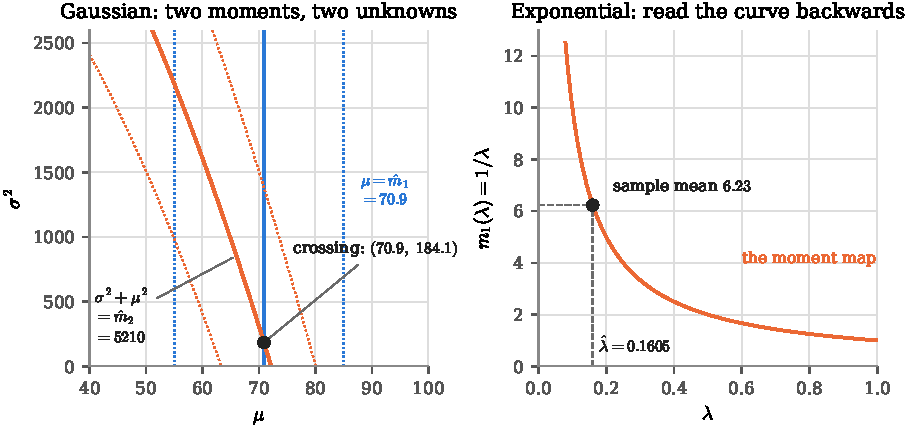
\includegraphics[width=\textwidth]{fig_mom_matching}
\caption{Left: the Gaussian moment map, with the parameters having the Old Faithful sample mean (blue) and sample mean square (orange) crossing at the estimate; dotted: other values of $m_1$ and $m_2$. Right: the exponential moment map $m_1 = 1/\lambda$, read backwards from the subway sample mean.}
\label{fig:mommatching}
\end{figure}

\begin{worked}[method of moments for the standard families]
\begin{itemize}
\item \textbf{Bernoulli.} $m_1(p) = p$, so $\hat{p} = \bar{X}_n$.
\item \textbf{Poisson.} $m_1(\lambda) = \lambda$, so $\hat{\lambda} = \bar{X}_n$. For the siblings data with $X - 1 \sim \Pois(\lambda)$, $m_1 = \lambda + 1$ and $\hat{\lambda} = \bar{X}_n - 1 = 1.0$, which is how \cref{ch:models} fitted it in the first place.
\item \textbf{Exponential.} $m_1(\lambda) = 1/\lambda$, so $\hat{\lambda} = 1/\bar{X}_n$.
\item \textbf{Gaussian.} $m_1 = \mu$ and $m_2 = \sigma^2 + \mu^2$. Solving, $\hat{\mu} = \hat{m}_1 = \bar{X}_n$ and $\widehat{\sigma^2} = \hat{m}_2 - \hat{m}_1^2 = \frac1n\sum_i X_i^2 - \bar{X}_n^2 = \frac1n\sum_i (X_i - \bar{X}_n)^2$: the divide-by-$n$ variance, which is the MLE as well.
\item \textbf{Uniform.} For $\Unif([0, \theta])$, $m_1 = \theta/2$, so $\hat{\theta}^{\text{MM}} = 2\bar{X}_n$. This one differs from the MLE $\max_i X_i$, and it can be absurd: for the five observations of \cref{fig:uniformlik}, with mean $4.84$, it gives $9.68$, which is fine, but a sample of $1, 1, 1, 1, 7.6$ gives $4.64$, below an observation the model then calls impossible.
\end{itemize}
For the Bernoulli, Poisson, exponential and Gaussian families the method of moments is the maximum likelihood estimator; for the uniform it is not, and for the Laplace model of \cref{ex:lik-laplace} the method of moments gives the sample mean while maximum likelihood gives the median.
The agreement for the first four is not a coincidence, and \cref{ch:exp-families} explains it: in an exponential family the likelihood equations match the moments of the sufficient statistics, which for these four families are the moments of $X$ itself.
\end{worked}

\begin{bridge}[the method of moments is how your first statistics course estimated everything]
An introductory course estimates a population mean by the sample mean, a variance by the sample variance, a proportion by the sample proportion, a correlation by the sample correlation.
Each of those is the method of moments: a population quantity written in terms of moments, with sample moments plugged in.
Karl Pearson named the method in 1894, before maximum likelihood existed, and it is still the first thing to try when a model's likelihood is awkward, since solving $d$ polynomial equations is usually easier than maximizing a function.
What the introductory course did not say is how precise the plug-in is, which is the next section.
\end{bridge}

\subsection{Asymptotic variance of the method of moments}
\label{sec:mom-variance}

\recall{The delta method (\cref{thm:delta}): if $\sqrt{n}(Z_n - \theta) \convd \Gauss(0, \sigma^2)$ and $g$ is continuously differentiable at $\theta$, then $\sqrt{n}(g(Z_n) - g(\theta)) \convd \Gauss(0, g'(\theta)^2\sigma^2)$. The Central Limit Theorem (\cref{thm:clt}): for i.i.d.\ $Y_i$ with mean $m$ and variance $s^2 < \infty$, $\sqrt{n}(\bar{Y}_n - m) \convd \Gauss(0, s^2)$. Slutsky's theorem (\cref{thm:slutsky}): if $X_n \convd X$ and $Y_n \convp y$, then $X_n Y_n \convd yX$ and, for $y \neq 0$, $X_n/Y_n \convd X/y$. Vector versions (the vector-versions remark of \cref{ch:limit-tools}): for i.i.d.\ vectors $V_i$ with mean $m$ and finite covariance matrix $\Sigma$, $\sqrt{n}(\bar{V}_n - m) \convd \Gauss_d(0, \Sigma)$, a Gaussian vector, meaning that every linear combination $a^\top Z$ of its coordinates is Gaussian, with variance $a^\top\Sigma a$; and for $g: \real^d \to \real^d$ continuously differentiable at $m$ with Jacobian matrix $G$ (row $j$ is the gradient of the $j$th coordinate of $g$), $\sqrt{n}(g(\bar{V}_n) - g(m)) \convd \Gauss_d(0, G\Sigma G^\top)$.}

A method of moments estimator is a function, $M^{-1}$, of sample moments, and sample moments are averages.
So the CLT gives the limit of the moments and the delta method carries it through $M^{-1}$.

\begin{theorem}[Asymptotic normality of the method of moments]
\label{thm:mom-normal}
Suppose $\Xton \iid \Pr_{\theta^*}$, the moment map $M$ is one-to-one, its image $M(\Theta)$ contains a neighborhood of $M(\theta^*)$ (so that the estimator exists for sample moments near the population ones), $M^{-1}$ is continuously differentiable at $M(\theta^*)$, and $\E_{\theta^*}[X^{2d}] < \infty$.
Let $\Sigma(\theta^*)$ be the $d \times d$ covariance matrix of the vector $(X, X^2, \ldots, X^d)$ under $\Pr_{\theta^*}$, and $\nabla M^{-1}$ the Jacobian matrix of $M^{-1}$ at $M(\theta^*)$: the $d \times d$ matrix whose row $j$ is the gradient of the $j$th coordinate of $M^{-1}$ (the transpose of the matrix in the vector-versions remark of \cref{ch:limit-tools}, which puts the coordinates in columns).
Then
\[
\sqrt{n}\,\big(\hat{\theta}_n^{\text{MM}} - \theta^*\big) \convd \Gauss_d\big(0, \Gamma(\theta^*)\big), \qquad \Gamma(\theta^*) = \nabla M^{-1}\,\Sigma(\theta^*)\,(\nabla M^{-1})^\top.
\]
For $d = 1$: $\Gamma = \big((M^{-1})'(m_1)\big)^2 \var_{\theta^*}(X)$.
\end{theorem}

\optionalproof{The vector of sample moments is an average of i.i.d.\ vectors, so the multivariate CLT gives $\sqrt{n}(\hat{m} - M(\theta^*)) \convd \Gauss_d(0, \Sigma)$. The estimator is $M^{-1}(\hat{m})$, and the multivariate delta method pushes the Gaussian through $M^{-1}$: the covariance gets multiplied by the derivative matrix on both sides.}
\begin{proof}
The $i$th observation contributes the vector $(X_i, X_i^2, \ldots, X_i^d)$; these vectors are i.i.d.\ with mean $M(\theta^*)$ and covariance $\Sigma(\theta^*)$, finite by the moment condition, and $\hat{m} = (\hat{m}_1, \ldots, \hat{m}_d)$ is their average.
The multivariate CLT of the recall gives $\sqrt{n}(\hat{m} - M(\theta^*)) \convd \Gauss_d(0, \Sigma(\theta^*))$.
For $d = 1$ the delta method applied to $g = M^{-1}$ finishes the proof.
For general $d$, the multivariate delta method is the same argument coordinate by coordinate: the mean value theorem writes $M^{-1}(\hat{m}) - M^{-1}(M(\theta^*))$ as a matrix of derivatives, evaluated at in-between points that converge to $M(\theta^*)$, times $\hat{m} - M(\theta^*)$; the derivative matrix converges in probability to $\nabla M^{-1}$ by continuity, and Slutsky's theorem (\cref{thm:slutsky}) multiplies it into the Gaussian limit.
A matrix $A$ times a Gaussian vector $Z$ with covariance $\Sigma$ is Gaussian with covariance $A\Sigma A^\top$: each linear combination $a^\top AZ = (A^\top a)^\top Z$ is Gaussian with variance $a^\top A \Sigma A^\top a$, and when $A$ is invertible, the linear-map rule of the Toolkit \toolkit{sec:math-gaussquad} shows that $AZ$ is $\Gauss_d(0, A\Sigma A^\top)$ in the sense defined there.
\end{proof}

\begin{worked}[the exponential rate, both ways]
For $\Expo(\lambda)$, $M(\lambda) = 1/\lambda$, $M^{-1}(m) = 1/m$ and $(M^{-1})'(m) = -1/m^2$, which at $m = 1/\lambda$ is $-\lambda^2$.
With $\var(X) = 1/\lambda^2$, the theorem gives asymptotic variance $\lambda^4 \cdot \lambda^{-2} = \lambda^2$: the same as the maximum likelihood estimator's $1/I(\lambda) = \lambda^2$ from \cref{ch:mle-properties}, as it must be, since the two estimators are the same function of the data.
For the subway, standard error $\hat{\lambda}/\sqrt{n} = 0.020$ once more.
\end{worked}

\begin{sanitycheck}[Could a different moment do better?]
The Poisson model has $m_1 = \lambda$, and also $m_2 = \lambda + \lambda^2$.
Nothing in the definition says you must use the first moment; you could match the second instead, solving $\hat{m}_2 = \lambda + \lambda^2$ for $\lambda = \big(-1 + \sqrt{1 + 4\hat{m}_2}\big)/2$.
Is that any better?
The theorem says no.
With $g(m) = (-1 + \sqrt{1 + 4m})/2$, $g'(m_2) = 1/(2\lambda + 1)$, and $\var(X^2) = \lambda + 6\lambda^2 + 4\lambda^3$ for a Poisson, so the asymptotic variance is $(\lambda + 6\lambda^2 + 4\lambda^3)/(2\lambda + 1)^2$, which at $\lambda = 1$ is $11/9 = 1.22$ against $\lambda = 1$ for the sample mean.
The second-moment estimator is $22\%$ noisier.
It throws away information by squaring, and an estimator built on higher moments is usually worse than one built on lower ones, since higher sample moments have larger variance (usually, not always: the derivative of $M^{-1}$ matters as much as the variance of the moment).
\end{sanitycheck}

\begin{proposition}[Method of moments is never better than maximum likelihood]
\label{prop:mom-vs-mle}
In a regular model (\cref{sec:mle-regularity}), under the hypotheses of \cref{thm:mom-normal}, the asymptotic variance of the method of moments estimator is at least that of the maximum likelihood estimator: $\Gamma(\theta^*) \geq 1/I(\theta^*)$ for $d = 1$, and in general $\Gamma - I^{-1}$ is positive semidefinite, meaning $a^\top(\Gamma - I^{-1})a \geq 0$ for every vector $a$: no linear combination of the parameters is estimated more precisely by moments than by likelihood.
\end{proposition}

\optionalproof{The delta step of \cref{thm:mom-normal} writes the method of moments estimator as an average plus a negligible term, and the score is an average too. The multivariate CLT makes the pair jointly Gaussian in the limit, their covariance works out to the identity by the same differentiate-under-the-integral step as in Cram\'er--Rao, and a variance is never negative.}
\begin{proof}
Take $d = 1$ first.
Write $T_n = \hat{\theta}_n^{\text{MM}}$ and $c = (M^{-1})'(m_1(\theta^*))$.
The mean value theorem step in the proof of \cref{thm:mom-normal} gives
\[
\sqrt{n}(T_n - \theta^*) = c\,\sqrt{n}(\hat{m}_1 - m_1(\theta^*)) + R_n, \qquad R_n \convp 0,
\]
since the derivative at the in-between point differs from $c$ by a quantity converging to zero in probability, multiplied by a sequence converging in distribution (Slutsky).
So $\sqrt{n}(T_n - \theta^*)$ is, up to $R_n$, the standardized average of the i.i.d.\ variables $U_i = c(X_i - m_1(\theta^*))$.
The score is the average of the i.i.d.\ variables $W_i = \ell'(\theta^*; X_i)$, with mean zero (\cref{prop:score-mean}) and variance $I(\theta^*)$ (\cref{def:fisher}).
Apply the multivariate CLT to the pairs $(U_i, W_i)$: the pair $\big(\sqrt{n}\bar{U}_n, \sqrt{n}\bar{W}_n\big)$ converges to a Gaussian vector $(U, W)$ with $\var(U) = \Gamma$, $\var(W) = I$ and
\begin{align*}
\cov(U, W) = \cov(U_1, W_1) &= c\,\E_{\theta^*}\!\big[X\,\ell'(\theta^*; X)\big] = c \int x\,\frac{\partial}{\partial\theta}p_{\theta}(x)\Big|_{\theta^*}\,\mathrm{d}x \\
&= c\,\frac{\mathrm{d}}{\mathrm{d}\theta}m_1(\theta)\Big|_{\theta^*} = c\,M'(\theta^*) = 1,
\end{align*}
where the mean-zero score let us drop $m_1(\theta^*)$, the exchange of derivative and integral is the regularity condition used in \cref{thm:cramer-rao}, and the last step is the inverse function rule $(M^{-1})'(M(\theta^*)) = 1/M'(\theta^*)$.
Adding $R_n$ does not change the limit (Slutsky).
Now $\var(U - W/I) = \Gamma - 2\cdot\frac{1}{I} + \frac{I}{I^2} = \Gamma - \frac1I \geq 0$, which is the claim.

For general $d$ the same steps give a Gaussian vector $(U, W)$ in $\real^{2d}$, with $U$ having covariance $\Gamma$, $W$ the score vector with covariance $I$, and $\cov(U, W) = \nabla M^{-1}\,\nabla M = $ the identity matrix, since the matrix of $\partial m_k/\partial\theta_j$ is the Jacobian $\nabla M$ and the inverse function rule inverts it.
For any vector $a$, $\var\big(a^\top U - a^\top I^{-1}W\big) = a^\top\Gamma a - 2a^\top I^{-1}a + a^\top I^{-1}II^{-1}a = a^\top(\Gamma - I^{-1})a \geq 0$.
\end{proof}

So when maximum likelihood is available, it is at least as precise.
The method of moments is the tool elsewhere: when the likelihood has no tractable maximum (the mixture of \cref{sec:lik-em} is a classic case, and Pearson's 1894 paper fitted a mixture of two Gaussians by matching five moments), or when it is the same estimator anyway and the moment version is easier to compute.

\section{M-estimation}
\label{sec:mest}

Both recipes so far minimized something.
Maximum likelihood minimized $-\frac1n\sum_i\log p_\theta(X_i)$.
The method of moments, for $d = 1$, solves $\hat{m}_1 = m_1(\theta)$, which is where $\frac1n\sum_i(X_i - m_1(\theta))^2$ has zero derivative with respect to $m_1$.
Here is the general pattern.

\begin{definition}[M-estimator]
\label{def:mest}
Let $\Xton$ be i.i.d.\ from a distribution $\Pr$ on $E$, and let $\mu^* \in \mathcal{M} \subset \real^d$ be a quantity attached to $\Pr$ that you want to estimate.
A \textbf{loss function} for $\mu^*$ is a function $\rho: E \times \mathcal{M} \to \real$ with $\E\abs{\rho(X, \mu)} < \infty$ for every $\mu$, such that the \textbf{expected loss}
\[
Q(\mu) = \E\big[\rho(X, \mu)\big]
\]
is smallest at $\mu = \mu^*$, and only there.
The \textbf{M-estimator} of $\mu^*$ is the minimizer of the \textbf{empirical loss},
\[
\hat{\mu}_n = \operatorname*{argmin}_{\mu \in \mathcal{M}} Q_n(\mu), \qquad Q_n(\mu) = \frac1n\sum_{i=1}^n \rho(X_i, \mu).
\]
\end{definition}

\begin{inwords}
\textbf{In words.} You want a number attached to the distribution: its mean, its median, a parameter. Find a loss that charges each observation according to how far it is from a candidate $\mu$, chosen so that the average charge over the whole distribution is smallest at the number you want. You cannot compute that average, but the LLN says the average over the data is close to it, so minimize the data's average instead. No statistical model is needed: the recipe asks only that $Q$ have its minimum at $\mu^*$.
\par\smallskip
\textbf{For the kiss data.} With $\rho(r, \mu) = (r - \mu)^2$, $Q(\mu) = \E[(R - \mu)^2] = \var(R) + (p - \mu)^2$ is smallest at $\mu = p$, and $Q_n(\mu) = \frac1n\sum_i(R_i - \mu)^2$ is smallest at $\bar{R}_n = 0.645$. The sample proportion is an M-estimator for the squared loss, which is its fourth derivation in this book.
\end{inwords}

\begin{worked}[losses and what they estimate]
\begin{itemize}
\item \textbf{Squared loss, $\rho(x, \mu) = (x - \mu)^2$.} $Q(\mu) = \var(X) + (\E[X] - \mu)^2$, minimized at $\mu^* = \E[X]$ (when $\var(X) < \infty$). The M-estimator is the sample mean: for the Old Faithful waits, $Q_n$ is minimized at $70.9$ minutes, the blue dot in \cref{fig:mestlosses}. In $\real^d$, with $\rho = \norm{x - \mu}^2$, it is the vector of sample means.
\item \textbf{Absolute loss, $\rho(x, \mu) = \abs{x - \mu}$.} $Q(\mu) = \E\abs{X - \mu}$ is minimized at a median of $X$ (\cref{prop:median-min}; this needs $\E\abs{X} < \infty$, and \cref{sec:mest-robust} says what to do when that fails). The M-estimator is the sample median.
\item \textbf{Check loss, $\rho(x, \mu) = C_\alpha(x - \mu)$ with $C_\alpha(u) = \alpha u$ for $u \geq 0$ and $-(1 - \alpha)u$ for $u < 0$.} A tilted absolute value, charging $\alpha$ per unit above $\mu$ and $1 - \alpha$ per unit below. $Q$ is minimized at the point with probability $\alpha$ below it, the $\alpha$-quantile (\cref{ex:mest-quantile}). The M-estimator is the sample quantile. With $\alpha = \frac12$ it is the median again.
\item \textbf{Negative log-likelihood, $\rho(x, \theta) = -\log p_\theta(x)$,} in a model with $\Pr = \Pr_{\theta^*}$. $Q(\theta) = -\E_{\theta^*}[\log p_\theta(X)] = \KL(\Pr_{\theta^*}, \Pr_\theta) + \text{constant}$, minimized at $\theta^*$ when the model is identifiable (\cref{ch:distances}). The M-estimator is the MLE.
\item \textbf{Huber's loss,} $\rho(x, \mu) = h_\delta(x - \mu)$ with $h_\delta(u) = u^2/2$ for $\abs{u} \leq \delta$ and $\delta(\abs{u} - \delta/2)$ beyond. Quadratic near zero, linear far away. For a symmetric distribution $Q$ is minimized at the center. \Cref{sec:mest-robust} says what it is for.
\end{itemize}
\end{worked}

\Cref{fig:mestlosses} draws three of the losses and their empirical versions on the Old Faithful waits.
The squared loss is a parabola in the residual (drawn as $\frac12(x - \mu)^2$, so that it and Huber's loss coincide on $[-\delta, \delta]$; halving a loss changes neither its minimizer nor, as \cref{sec:mest-normal} shows, the variance of its M-estimator); the absolute loss is a V; Huber's is the parabola inside $[-\delta, \delta]$ and the V's straight sides outside, where the blue and aqua curves separate.
On the right, each empirical loss is minimized at a different center of the same data: the squared loss at the mean, $70.9$ minutes; the absolute loss at the median, $76$; Huber's loss with $\delta = 5$ minutes at $75.0$, between the two.
The data are not symmetric (the two humps of \cref{fig:emfaithful} have unequal weights), so the three `centers' are three different numbers, each the right answer to its own loss.

\begin{figure}[htbp]
\centering
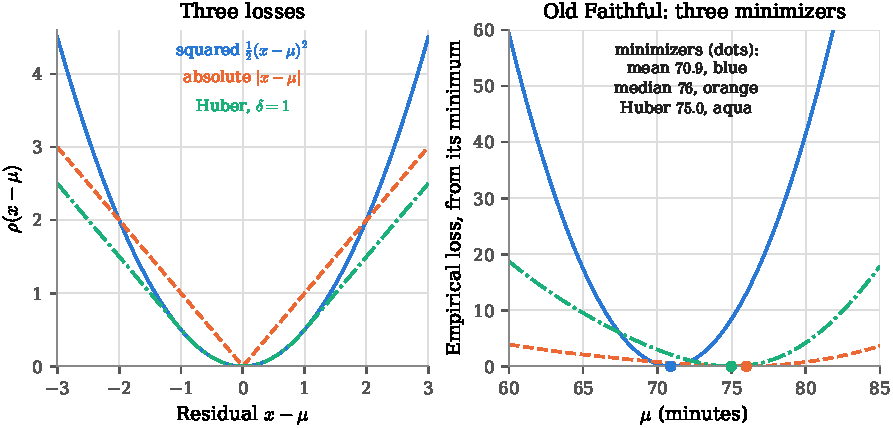
\includegraphics[width=\textwidth]{fig_mestimation_losses}
\caption{Left: the squared (blue), absolute (orange, dashed) and Huber (aqua, dash-dot, $\delta = 1$) losses as functions of the residual. Right: the three empirical losses for the Old Faithful waits, each measured from its minimum, with the minimizers marked.}
\label{fig:mestlosses}
\end{figure}

\begin{proposition}[The median minimizes expected absolute deviation]
\label{prop:median-min}
Let $X$ have $\E\abs{X} < \infty$ and a continuous density $f$, and let $m$ be a median, $\Pr(X < m) = \Pr(X > m) = \frac12$.
Then $Q(\mu) = \E\abs{X - \mu}$ is minimized at $\mu = m$, and at no other point if $f(m) > 0$.
\end{proposition}

\coreproof{The derivative of $Q$ at $\mu$ is the probability below $\mu$ minus the probability above it: each unit you move $\mu$ to the right, the observations below it each cost one more and those above each cost one less. That derivative is negative below the median, zero at it and positive above.}
\begin{proof}
Split the expectation at $\mu$:
\[
Q(\mu) = \int_\mu^\infty (x - \mu)f(x)\,\mathrm{d}x + \int_{-\infty}^\mu (\mu - x)f(x)\,\mathrm{d}x.
\]
Differentiate in $\mu$. The first integral has derivative $-\int_\mu^\infty f(x)\,\mathrm{d}x$ (the integrand's derivative in $\mu$ is $-f$, and the boundary term $(\mu - \mu)f(\mu)$ is $0$); the second has derivative $\int_{-\infty}^\mu f(x)\,\mathrm{d}x$ by the same reasoning \toolkit{sec:math-density}.
So
\[
Q'(\mu) = \Pr(X < \mu) - \Pr(X > \mu) = 2F(\mu) - 1,
\]
where $F$ is the CDF.
This is at most $0$ for $\mu < m$, zero at $m$ and at least $0$ for $\mu > m$, so $Q$ decreases until $m$ and increases after: $m$ is a minimizer. If $f(m) > 0$, then $F$ is strictly increasing near $m$, so $Q'$ is strictly negative just below $m$ and strictly positive just above, and $m$ is the only minimizer (the Laplace and Gaussian densities are positive everywhere, so this applies to them).
\end{proof}

\begin{sanitycheck}[Is the kiss proportion a median too?]
The median of $\Bern(0.645)$ is $1$: more than half the mass sits there.
So the absolute loss, which estimates the median, would estimate `$1$' for the kiss experiment, and indeed the sample median of $80$ ones and $44$ zeros is $1$.
That is correct and useless.
A loss chooses what it estimates (an M-estimator estimates whatever its $Q$ is minimized at), and for a proportion the squared loss, which estimates the mean $p$, is the one that answers the question.
\end{sanitycheck}

\subsection{Asymptotic normality of M-estimators}
\label{sec:mest-normal}

The argument of \cref{ch:mle-properties} used only that the log-likelihood is a sum of i.i.d.\ terms.
Every empirical loss is one, so the argument goes through, with one change: the two roles the Fisher information played, as the variance of the score and as the curvature, are now played by two different numbers.

\begin{definition}[The $J$ and $K$ of a loss]
\label{def:jk}
For a loss $\rho$ twice differentiable in $\mu$, with $\mu \in \real^d$, define
\[
J(\mu) = \E\big[\nabla^2_\mu\,\rho(X, \mu)\big], \qquad K(\mu) = \mathrm{Cov}\big(\nabla_\mu\,\rho(X, \mu)\big),
\]
the expected Hessian of the loss (the curvature of $Q$ at $\mu$) and the covariance matrix of its gradient (as the Fisher information matrix of \cref{def:fisher} is the covariance of the score). For $d = 1$ they are $J(\mu) = \E[\partial^2_\mu\rho(X, \mu)]$ and $K(\mu) = \var(\partial_\mu\rho(X, \mu))$.
\end{definition}

\begin{inwords}
\textbf{In words.} $K$ is how much one observation's push on the estimate varies: the analogue of the variance of the score. $J$ is how hard the expected loss resists being pushed: the analogue of the curvature. For the negative log-likelihood the two coincide and both equal the Fisher information, by \cref{thm:fisher-curvature}; for any other loss they are different numbers.
\par\smallskip
\textbf{For the kiss data.} With the squared loss, $\partial_\mu\rho = -2(R - \mu)$ and $\partial^2_\mu\rho = 2$, so $J = 2$ and $K = 4\var(R) = 4p(1 - p)$: at $p = 0.645$, $K = 0.916$.
\end{inwords}

\recall{\Cref{thm:mle-normal} and its proof: for an estimator defined by $\sum_i g_i'(\hat{\mu}) = 0$, the mean value theorem writes $0 = \sum_i g_i'(\mu^*) + \sum_i g_i''(\tilde{\mu})(\hat{\mu} - \mu^*)$; the CLT handles the first sum, the LLN the second, Slutsky the ratio.}

\begin{theorem}[Asymptotic normality of M-estimators]
\label{thm:mest-normal}
Let $\Xton$ be i.i.d.\ from $\Pr$ and let $\mu^*$ be the unique minimizer of $Q$, in the interior of $\mathcal{M}$ (the analogue of condition 3 of \cref{sec:mle-regularity}).
Suppose the hypotheses of \cref{thm:mle-consistent} hold with $\rho$ in place of $-\log p_\theta$ (a bounded closed $\mathcal{M}$, or the restriction argument given there; $\rho$ continuous in $\mu$; $\E[\sup_\mu\abs{\rho(X, \mu)}] < \infty$), so that $\hat{\mu}_n \convp \mu^*$.
Suppose also that $\rho$ is three times differentiable in $\mu$ near $\mu^*$, that derivatives in $\mu$ can be moved inside $\E$ at $\mu^*$, that $K(\mu^*)$ and $\E[\partial^2_\mu\rho(X, \mu^*)]$ are finite with $J(\mu^*)$ invertible (the analogue of condition 5), and that $\abs{\partial^3_\mu\rho(X, \mu)} \leq B(X)$ near $\mu^*$ for some $B$ with $\E[B(X)] < \infty$ (the analogue of condition 4).
Then
\[
\sqrt{n}\,(\hat{\mu}_n - \mu^*) \convd \Gauss_d\Big(0,\; J(\mu^*)^{-1}K(\mu^*)J(\mu^*)^{-1}\Big).
\]
For $d = 1$ the asymptotic variance is $K(\mu^*)/J(\mu^*)^2$.
\end{theorem}

\optionalproof{Word for word the proof of \cref{thm:mle-normal}, with $\rho$ in place of $-\log p_\theta$. The gradient of the empirical loss is zero at $\hat{\mu}_n$ and, by the CLT, approximately $\Gauss(0, K/n)$ at $\mu^*$ (its mean is zero there because $\mu^*$ minimizes $Q$). The curvature between is about $J$ by the LLN. Displacement is push over resistance: $(\text{sd } \sqrt{K/n})/J$.}
\begin{proof}
Consistency is \cref{thm:mle-consistent} with $-\log p_\theta$ replaced by $\rho$: the proof there used the uniform LLN and the unique minimizer of the limit, and nothing about the likelihood.
For normality, take $d = 1$.
Since $\mu^*$ minimizes $Q$ and is interior, $Q'(\mu^*) = \E[\partial_\mu\rho(X, \mu^*)] = 0$ (differentiating under the expectation, which the regularity conditions allow).
So the terms $\partial_\mu\rho(X_i, \mu^*)$ are i.i.d.\ with mean $0$ and variance $K(\mu^*)$, and the CLT gives $\frac{1}{\sqrt{n}}\sum_i\partial_\mu\rho(X_i, \mu^*) \convd \Gauss(0, K(\mu^*))$.
Since $\hat{\mu}_n$ is interior with probability tending to $1$, $Q_n'(\hat{\mu}_n) = 0$, and the mean value theorem gives a $\tilde{\mu}_n$ between $\hat{\mu}_n$ and $\mu^*$ with
\[
0 = Q_n'(\hat{\mu}_n) = Q_n'(\mu^*) + Q_n''(\tilde{\mu}_n)(\hat{\mu}_n - \mu^*), \qquad\text{so}\qquad \sqrt{n}(\hat{\mu}_n - \mu^*) = -\,\frac{\sqrt{n}\,Q_n'(\mu^*)}{Q_n''(\tilde{\mu}_n)}.
\]
The numerator is $\frac{1}{\sqrt{n}}\sum_i\partial_\mu\rho(X_i, \mu^*)$, which converges in distribution to $\Gauss(0, K)$.
The denominator is $Q_n''(\tilde{\mu}_n) = \frac1n\sum_i\partial^2_\mu\rho(X_i, \tilde{\mu}_n)$. It converges in probability to $J(\mu^*)$ by the LLN at $\mu^*$ and the bound $B$ on the third derivative, used exactly as $K$ was in the proof of \cref{thm:mle-normal}: the difference between the average second derivative at $\tilde{\mu}_n$ and at $\mu^*$ is at most $\bar{B}_n\abs{\hat{\mu}_n - \mu^*}$, an average converging to $\E[B(X)]$ times a quantity converging to $0$.
Slutsky's theorem gives the limit $-\Gauss(0, K)/J = \Gauss(0, K/J^2)$ (the sign is absorbed, since $-Z$ has the same distribution as $Z$).
In $d$ dimensions the denominator is the matrix $J$, inverted, applied to a Gaussian vector of covariance $K$, giving $J^{-1}KJ^{-1}$.
\end{proof}

\begin{intuition}[why the variance has three factors]
For maximum likelihood the push and the resistance were the same number, $I$, and push over resistance gave $\sqrt{I}/I = 1/\sqrt{I}$.
For a general loss they come apart.
The push has standard deviation $\sqrt{K}$; the resistance is $J$; the displacement has standard deviation $\sqrt{K}/J$, and its variance is $K/J^2$.
In matrix form that is $J^{-1}KJ^{-1}$, the curvature inverted on both sides of the push's covariance, which is why it is called the \textbf{sandwich}.
A loss with a stiff $Q$ (large $J$) and a quiet gradient (small $K$) gives a precise estimator.
\end{intuition}

\begin{worked}[the sandwich for the sample mean]
With the squared loss, $J = 2$ and $K = 4\var(X)$, so the asymptotic variance is $4\var(X)/4 = \var(X)$: the CLT for the sample mean, recovered. For the kiss data, $p(1 - p) = 0.229$.
\end{worked}

\begin{worked}[the Laplace median has asymptotic variance $1$]
\label{wk:laplace-median}
Let $\Xton$ have the Laplace density $f(x) = \frac12 e^{-\abs{x - m}}$ of \cref{ex:lik-laplace}, and estimate the center $m$ by the sample median, the M-estimator for $\rho = \abs{x - \mu}$.
The absolute value has a corner, so \cref{def:jk} does not apply directly; the way around is to compute $J$ as the curvature of $Q$ itself.
From the proof of \cref{prop:median-min}, $Q'(\mu) = 2F(\mu) - 1$, so $J = Q''(m) = 2f(m) = 2 \times \frac12 = 1$.
For $K$, $\partial_\mu\abs{X - \mu} = -\mathrm{sign}(X - \mu)$ away from the corner, which is $\pm 1$ with probability $\frac12$ each at $\mu = m$: variance $1$.
So the asymptotic variance is $K/J^2 = 1$.
The sample mean of Laplace data has asymptotic variance $\var(X) = 2$.
The median is twice as precise, and its standard error is $1/\sqrt{n}$ against the mean's $\sqrt{2/n}$.
(That the theorem's conclusion holds despite the corner is a separate argument, which this book does not reproduce; the formula $1/(4f(m)^2)$ for the median's asymptotic variance is standard.)
\end{worked}

\section{Robustness}
\label{sec:mest-robust}

\Cref{fig:robustmeanmedian} runs the sample mean and the sample median side by side on three symmetric distributions, $20{,}000$ samples of $n = 100$ each.
For Gaussian data the mean is the better estimator of the center: its standard deviation is $0.100$ against the median's $0.124$, matching the asymptotic variances $1$ and $\pi/2$ (the median's $1/(4f(0)^2)$ with $f(0) = 1/\sqrt{2\pi}$).
In about $61\%$ of samples the mean lands closer to the truth.
For Laplace data the order reverses, $0.141$ against $0.108$, and the median is closer in $62\%$ of samples. The mean's $0.141$ is exactly the $\sqrt{2/100}$ of the worked example; the median's $0.108$ is still $8\%$ above its asymptotic $1/\sqrt{100} = 0.100$, because the Laplace density has a corner at the center and the median's distribution approaches its Gaussian limit slowly there.
For Cauchy data, with density $f(x) = 1/(\pi(1 + (x - m)^2))$, the mean does not settle at all: its histogram is spread across the whole axis and beyond, with a standard deviation of $72$ over the $20{,}000$ samples, while the median's is $0.158$, close to its asymptotic $(\pi/2)/10 = 0.157$.

\begin{figure}[htbp]
\centering
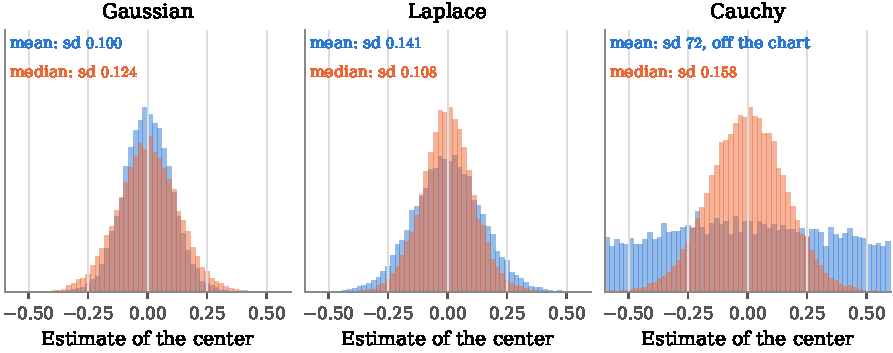
\includegraphics[width=\textwidth]{fig_robust_mean_median}
\caption{The sample mean (blue) and sample median (orange) of $n = 100$ observations, over $20{,}000$ samples, for Gaussian, Laplace and Cauchy data centered at $0$.}
\label{fig:robustmeanmedian}
\end{figure}

\begin{pitfall}[the Cauchy mean]
The Cauchy density has tails so heavy that $\E\abs{X} = \int\abs{x}f(x)\,\mathrm{d}x$ is infinite: the integrand behaves like $1/(\pi\abs{x})$ for large $\abs{x}$, and $\int_1^A \mathrm{d}x/x = \log A \to \infty$.
The mean does not exist, the LLN's hypothesis fails, and the sample mean does not converge to anything.
Worse, the average of $n$ Cauchy observations has exactly the same Cauchy distribution as a single observation: averaging $100$ of them buys nothing.
The method of moments is unavailable (no moments), the sample mean is useless, and the median, the MLE and Huber's estimator all work, with the Cauchy MLE of the center attaining the Cram\'er--Rao variance $2$, against the median's $\pi^2/4 = 2.47$. (Since $\E\abs{X} = \infty$, the absolute loss has infinite expectation here and \cref{def:mest} does not literally apply; the fix is the loss $\abs{x - \mu} - \abs{x}$, which is bounded by $\abs{\mu}$, has finite expectation for every distribution, and has the same minimizer and the same M-estimator, since subtracting $\abs{x}$ shifts $Q_n$ by a constant.)
\end{pitfall}

An estimator that keeps working when the data have heavy tails, or when a few observations are wrong (a decimal point in the wrong place, a sensor fault), is called \textbf{robust}.
The sample median is the simplest robust estimator of a center: move the largest observation to $10^{10}$ and the median does not change, while the mean goes to infinity.
Its price is efficiency on clean Gaussian data, where it is $\pi/2 = 1.57$ times noisier than the mean, so that it needs $57\%$ more observations for the same precision.
Huber's loss is the compromise.

\begin{intuition}[Huber's loss: a mean in the middle, a median in the tails]
$h_\delta(u)$ is $u^2/2$ for $\abs{u} \leq \delta$ and $\delta(\abs{u} - \delta/2)$ beyond, joined so that the function and its slope are continuous (\cref{fig:mestlosses}, left).
Its derivative is the \textbf{clip} function: $u$ inside $[-\delta, \delta]$ and $\pm\delta$ outside.
So an observation within $\delta$ of the current center pushes it the way the squared loss would, in proportion to its distance, and an observation beyond $\delta$ pushes with the fixed force $\delta$, the way the absolute loss would, however far away it is.
A wild observation can push at most $\delta$: that is the robustness.
Observations in the bulk are treated as the mean treats them: that is the efficiency.
The constant $\delta$ sets where `the bulk' ends, and a common choice on data with scale $1$ is $\delta = 1.345$, which costs only $5\%$ in variance on Gaussian data ($1.05$ against the mean's $1$) while capping the influence of any observation.
\end{intuition}

\begin{worked}[Huber on Laplace data]
Take the Laplace center $m$ and $\rho(x, \mu) = h_\delta(x - \mu)$.
Huber's loss is twice differentiable except at $\pm\delta$, so \cref{def:jk} applies (as with the median, the kink means \cref{thm:mest-normal} does not literally cover it, and the standard argument that extends the theorem to this case is not reproduced here): $\partial^2_\mu\rho = \ind(\abs{X - \mu} \leq \delta)$, and
\[
J(m) = \Pr(\abs{X - m} \leq \delta) = \int_{-\delta}^\delta \tfrac12 e^{-\abs{u}}\,\mathrm{d}u = 1 - e^{-\delta}.
\]
The gradient $-\mathrm{clip}_\delta(X - \mu)$ has mean zero at $m$ by symmetry, and
\[
K(m) = \E\big[\mathrm{clip}_\delta(X - m)^2\big] = \int_{-\delta}^\delta u^2\,\tfrac12 e^{-\abs{u}}\,\mathrm{d}u + \delta^2\Pr(\abs{X - m} > \delta) = 2 - e^{-\delta}(2\delta + 2),
\]
the integral by two integrations by parts.
With $\delta = 1$: $J = 0.632$, $K = 0.528$ and the asymptotic variance $K/J^2 = 1.32$, between the median's $1$ and the mean's $2$.
As $\delta \to 0$ the variance tends to $1$ (Huber becomes the median) and as $\delta \to \infty$ it tends to $2$ (Huber becomes the mean); at $\delta = 0.5$ it is $1.17$, at $\delta = 2$ it is $1.59$.
\end{worked}

\begin{bridge}[trimmed means and `robust standard errors']
An introductory course may have mentioned the trimmed mean, the average after discarding the top and bottom $10\%$, as a compromise between mean and median.
Huber's estimator is the principled version: instead of discarding the extremes it caps their influence, and it comes with a standard error, $\sqrt{K/(nJ^2)}$ with $J$ and $K$ estimated from the data.
The sandwich formula also underlies the `robust' or `heteroskedasticity-consistent' standard errors of regression software: least squares is an M-estimator with the squared loss, and when the errors are not identically distributed $K$ is no longer a multiple of $J$, so the usual standard error ($\sigma^2$ times the inverse of $\E[XX^\top]$) is wrong and the sandwich $J^{-1}KJ^{-1}$ is right.
\Cref{ch:regression-multi} returns to this.
\end{bridge}

\section{What comes next}
\label{sec:mom-next}

Part IV is complete: three recipes, each consistent and asymptotically normal, each with a variance you can compute and plug in to get $\text{estimate} \pm 1.96\,\text{standard error}$.
Maximum likelihood has the smallest variance when the model is right; the method of moments is the same estimator for the common families and a fallback when the likelihood is awkward; M-estimation with a robust loss gives up a little precision for protection against heavy tails and bad data.
\Cref{ch:t-test} opens Part V by handling the one situation none of this covers, a small Gaussian sample where the limit theorems have not taken hold, with exact distributions in place of asymptotic ones.
\Cref{ch:wald-lrt} turns the asymptotic normality of \cref{ch:mle-properties} into tests.
\Cref{ch:exp-families} explains why the method of moments and maximum likelihood kept agreeing.

\section{Summary}
\label{sec:mom-summary}

\begin{itemize}[nosep]
\item Method of moments: $\hat{\theta}^{\text{MM}} = M^{-1}(\hat{m}_1, \ldots, \hat{m}_d)$, the parameter whose first $d$ moments match the sample's. Bernoulli, Poisson, exponential and Gaussian all give the MLE; $\Unif([0, \theta])$ gives $2\bar{X}_n$, not the MLE.
\item Its asymptotic variance, by the multivariate CLT and the delta method, is $\nabla M^{-1}\,\Sigma\,(\nabla M^{-1})^\top$; for $d = 1$, $((M^{-1})')^2\var(X)$. It is never below $1/I$. Higher moments make worse estimators ($11/9$ against $1$ for the Poisson rate).
\item M-estimator: $\hat{\mu}_n = \operatorname{argmin}\frac1n\sum_i\rho(X_i, \mu)$ for a loss whose expectation $Q$ is minimized at $\mu^*$. Squared loss gives the mean, absolute loss the median ($Q' = 2F - 1$), check loss the quantile, negative log-likelihood the MLE, Huber's loss a robust center.
\item Asymptotic variance $J^{-1}KJ^{-1}$ with $J = \E[\nabla^2\rho]$ (resistance) and $K = \mathrm{Cov}(\nabla\rho)$ (push); for the MLE $J = K = I$. Laplace median $1$ against mean $2$; Gaussian median $\pi/2$ against mean $1$; Huber with $\delta = 1$ on Laplace data $1.32$.
\item Cauchy data have no mean; the sample mean of $100$ of them is as noisy as one. The median, Huber and the MLE still work.
\end{itemize}

\section{Exercises}
\label{sec:mom-exercises}

\begin{exercise}
\label{ex:mom-gauss-data}
For the four observations $0.5, 1.8, -2.3, 0.9$ from a $\Gauss(\mu, \sigma^2)$ model, compute the method of moments estimates of $\mu$ and $\sigma$.
\end{exercise}
\begin{solution}
$\hat{m}_1 = (0.5 + 1.8 - 2.3 + 0.9)/4 = 0.225$ and $\hat{m}_2 = (0.25 + 3.24 + 5.29 + 0.81)/4 = 2.3975$. So $\hat{\mu} = 0.225$ and $\hat{\sigma} = \sqrt{2.3975 - 0.225^2} = \sqrt{2.347} = 1.532$. These are the MLEs as well; the divide-by-$(n-1)$ sample standard deviation would be $1.532\sqrt{4/3} = 1.769$.
\end{solution}

\begin{exercise}
\label{ex:mom-uniform}
For $\Xton \iid \Unif([0, \theta])$, find the method of moments estimator and its asymptotic variance, and compare its standard deviation at $n = 100$, $\theta = 10$ with the MLE's, whose error is about $\theta/n$ in size (\cref{ex:mle-uniform-rate}).
\end{exercise}
\begin{solution}
$m_1 = \theta/2$, so $\hat{\theta}^{\text{MM}} = 2\bar{X}_n$. With $M^{-1}(m) = 2m$ and $\var(X) = \theta^2/12$, the asymptotic variance is $4\theta^2/12 = \theta^2/3$, and the standard deviation at $n = 100$ is $\sqrt{100/3}/10 = 0.577$. The MLE's error is of order $\theta/n = 0.1$, six times smaller, and shrinking like $1/n$ rather than $1/\sqrt{n}$. The method of moments estimator is unbiased and asymptotically normal, and the MLE beats it anyway: the model is not regular, so the Cram\'er--Rao floor that would protect a regular MLE's variance does not exist here, and the MLE goes below it.
\end{solution}

\begin{exercise}
\label{ex:mom-gamma}
The Gamma family with shape $a > 0$ and rate $b > 0$ has $m_1 = a/b$ and $m_2 = a(a + 1)/b^2$. Find the method of moments estimators of $a$ and $b$. (The MLE of this family has no closed form, which is why the method of moments is used for it.)
\end{exercise}
\begin{solution}
From $m_2 - m_1^2 = a/b^2$ (the variance) and $m_1 = a/b$: dividing, $m_1/(m_2 - m_1^2) = b$, and then $a = m_1 b = m_1^2/(m_2 - m_1^2)$. So $\hat{b} = \hat{m}_1/(\hat{m}_2 - \hat{m}_1^2) = \bar{X}_n/\widehat{\sigma^2}$ and $\hat{a} = \bar{X}_n^2/\widehat{\sigma^2}$, with $\widehat{\sigma^2}$ the divide-by-$n$ sample variance. Two moments, two unknowns, solved in two lines; the likelihood equations involve the derivative of $\log\Gamma(a)$ and need a numerical solver.
\end{solution}

\begin{exercise}
\label{ex:mest-quantile}
Show that $Q(\mu) = \E[C_\alpha(X - \mu)]$, with the check loss $C_\alpha(u) = \alpha u$ for $u \geq 0$ and $-(1 - \alpha)u$ for $u < 0$, is minimized at the $\alpha$-quantile of a continuous $X$ with $\E\abs{X} < \infty$, the point $q$ with $F(q) = \alpha$.
\end{exercise}
\begin{solution}
$Q(\mu) = \alpha\int_\mu^\infty (x - \mu)f(x)\,\mathrm{d}x + (1 - \alpha)\int_{-\infty}^\mu (\mu - x)f(x)\,\mathrm{d}x$. Differentiating as in \cref{prop:median-min}, $Q'(\mu) = -\alpha\Pr(X > \mu) + (1 - \alpha)\Pr(X < \mu) = -\alpha(1 - F(\mu)) + (1 - \alpha)F(\mu) = F(\mu) - \alpha$. This is zero exactly when $F(\mu) = \alpha$, negative below and positive above, so the minimizer is the $\alpha$-quantile. With $\alpha = \frac12$, $Q' = F - \frac12$, half the median's $2F - 1$, and the same minimizer. (The quantile here is the point with probability $\alpha$ \textit{below} it; the book's $q_\alpha$ for Gaussian tails has probability $\alpha$ above, as \cref{ch:gaussian} explains.)
\end{solution}

\begin{exercise}
\label{ex:mest-gauss-median}
For Gaussian data with variance $\sigma^2$, compute the asymptotic variance of the sample median by the $1/(4f(m)^2)$ formula and compare it with the sample mean's. How many more observations does the median need for the same precision?
\end{exercise}
\begin{solution}
$f(m) = 1/(\sigma\sqrt{2\pi})$, so $1/(4f(m)^2) = 2\pi\sigma^2/4 = (\pi/2)\sigma^2 = 1.571\sigma^2$, against $\sigma^2$ for the mean. The median needs $\pi/2 - 1 = 57\%$ more observations. In the simulation of \cref{fig:robustmeanmedian}, $0.124/0.100 = 1.24 \approx \sqrt{\pi/2} = 1.253$.
\end{solution}

\begin{exercise}
\label{ex:mest-huber-gauss}
For Gaussian data with variance $1$ and Huber's loss with $\delta = 1.345$, $J = \Pr(\abs{Z} \leq \delta) = 2\Phi(\delta) - 1$ and $K = \E[\min(Z^2, \delta^2)]$. Given $J = 0.821$ and $K = 0.710$, compute the asymptotic variance and the efficiency relative to the sample mean.
\end{exercise}
\begin{solution}
$K/J^2 = 0.710/0.674 = 1.053$. The mean has asymptotic variance $1$, so Huber's estimator is $5.3\%$ noisier on clean Gaussian data, which is the price of capping every observation's influence at $\delta$. For $\delta = 1$ the figures are $J = 0.683$, $K = 0.516$ and variance $1.107$; for $\delta = 2$, variance $1.010$. The larger $\delta$, the closer to the mean in both efficiency and fragility.
\end{solution}

\begin{exercise}
\label{ex:mest-cauchy-avg}
Accept that the average of $n$ i.i.d.\ Cauchy observations has the same Cauchy distribution as one of them. Explain why this does not contradict the Law of Large Numbers or the Central Limit Theorem, and what it says about $\bar{X}_{1000}$ as an estimate of the center.
\end{exercise}
\begin{solution}
Both theorems assume a finite mean (the LLN as stated in this book assumes a finite variance). The Cauchy has neither: $\int\abs{x}f(x)\,\mathrm{d}x = \infty$. So the theorems say nothing, and the fact is consistent with them. $\bar{X}_{1000}$ is exactly as spread out as a single observation: its probability of landing within $1$ of the center is $\Pr(\abs{X_1 - m} \leq 1) = \frac12$, the same as for $n = 1$. A thousand observations averaged are worth one. The sample median of the same thousand has standard deviation about $\sqrt{\pi^2/4}/\sqrt{1000} = 0.050$.
\end{solution}

\begin{exercise}
\label{ex:mest-sandwich-mle}
Show that for the loss $\rho(x, \theta) = -\log p_\theta(x)$ in a regular model, $J(\theta^*) = K(\theta^*) = I(\theta^*)$, so that \cref{thm:mest-normal} reduces to \cref{thm:mle-normal}.
\end{exercise}
\begin{solution}
$\nabla_\theta\rho = -\nabla_\theta\log p_\theta(X)$, the negative score, whose covariance is the covariance of the score, $I(\theta^*)$ by \cref{def:fisher} (a sign flip does not change a covariance). $\nabla^2_\theta\rho = -\nabla^2_\theta\log p_\theta(X)$, whose expectation is $-\E[\nabla^2\ell] = I(\theta^*)$ by \cref{thm:fisher-curvature}. So $J = K = I$ and $J^{-1}KJ^{-1} = I^{-1}II^{-1} = I^{-1}$.
\end{solution}


\partintro{The tests of \cref{ch:tests-foundations} were built on one standardized average. This part supplies the distributions the remaining parametric tests use, chi-squared and Student's $t$, with Cochran's theorem behind them (\cref{ch:t-test}), and the three general-purpose tests built on the likelihood, Wald's, the likelihood ratio and the score test (\cref{ch:wald-lrt}).}
\part{Parametric Hypothesis Tests}
\chapter[The $t$-Test]{Chi-Squared, Student's $t$, Cochran's Theorem and the $t$-Test}
\label{ch:t-test}

% Not yet written. Source material: notes sections The Chi-Squared Distribution, The t-Test, Cochran's Theorem; unit 4 slides

\chapter{Wald and Likelihood Ratio Tests}
\label{ch:wald-lrt}

% Not yet written. Source material: notes sections Wald's Test, Recitation: Comparisons of Two Proportions; unit 4 slides (likelihood ratio test)


\partintro{Every method so far assumed the model was well-specified. This part tests that assumption: goodness of fit for discrete distributions by the chi-squared test (\cref{ch:gof}), and for continuous ones by comparing the empirical CDF with the candidate, the Kolmogorov--Smirnov and Lilliefors tests and the QQ plot (\cref{ch:ks}).}
\part{Nonparametric Hypothesis Tests}
\chapter{Goodness of Fit for Discrete Distributions}
\label{ch:gof}

% Not yet written. Source material: notes ch. Non-Parametric Hypothesis Tests; unit 5 slides

\chapter{Kolmogorov--Smirnov, Lilliefors and QQ Plots}
\label{ch:ks}

\begin{chaptergoals}
\begin{itemize}[nosep]
\item The empirical CDF, which estimates a whole distribution at once. At each point it is a sample proportion, so the Law of Large Numbers and the Central Limit Theorem apply point by point; the Glivenko--Cantelli theorem makes the first hold at all points at once, and Donsker's theorem does the same for the second.
\item The Kolmogorov--Smirnov test of a stated continuous distribution: the largest vertical gap between the empirical CDF and the candidate. Its null distribution is the same for every continuous candidate, so one table, or one simulation, serves them all.
\item Other measures of the gap, Cram\'er--von Mises and Anderson--Darling, and what binning the data for a chi-squared test gives up.
\item Testing a family: estimating its parameters changes the null distribution, and the Kolmogorov--Smirnov table then gives a test that almost never rejects. The Lilliefors test for normality is the repair.
\item QQ plots: the same comparison drawn as quantiles against quantiles, and how to read heavy tails, light tails and skew from one. Newcomb's measurements of the speed of light and the eruptions of Old Faithful.
\end{itemize}
\Cref{ch:gof} tested distributions on finitely many categories by counting. This chapter tests continuous distributions without grouping the data at all.
\end{chaptergoals}

\section{The empirical CDF}
\label{sec:ks-ecdf}

A continuous distribution has no natural categories.
\Cref{ch:gof} could still test one by cutting the line into cells and counting, but the answer depends on where the cuts go, and each observation is reduced to the name of its cell.
The object that describes a distribution on the line without any cutting is its CDF, $F(t) = \Pr(X \leq t)$, and it has an obvious estimate: the proportion of the sample at or below $t$.

\begin{definition}[The empirical CDF]
\label{def:ecdf}
For a sample $\Xton$, the \textbf{empirical CDF} is the random function
\[
F_n(t) = \frac1n\sum_{i=1}^n \ind(X_i \leq t) = \frac{\#\{i : X_i \leq t\}}{n}, \qquad t \in \real.
\]
With the observations sorted, $X_{(1)} \leq X_{(2)} \leq \cdots \leq X_{(n)}$ (the \textbf{order statistics}), $F_n$ is a staircase that is $0$ below $X_{(1)}$, climbs $1/n$ at each observation, and is $1$ from $X_{(n)}$ on.
\end{definition}

\begin{inwords}
\textbf{In words.} At each $t$, count the observations at or below $t$ and divide by $n$ \toolkit{sec:math-indicator}. The result is the CDF of the distribution that puts probability $1/n$ on each data point.
\par\smallskip
\textbf{For the kiss data.} With $R_i = 1$ for a right turn, $F_n(t)$ is $0$ for $t < 0$, $44/124 = 0.355$ for $0 \leq t < 1$, and $1$ from $t = 1$ on. Its step at $1$ has height $\hat{p} = 0.645$: for two-valued data the empirical CDF carries exactly the information in $\hat{p}$.
\end{inwords}

The left of \cref{fig:ecdfgc} shows two empirical CDFs of simulated waits from the exponential distribution with mean $6.23$ minutes, the model of the subway data, against the true CDF.
With $10$ observations the staircase is coarse and strays as far as $0.25$ from the curve; with $100$ it stays within about $0.08$.

\recall{The Law of Large Numbers (\cref{thm:wlln}): for i.i.d.\ random variables with mean $\mu$ and finite variance, $\bar{X}_n \convp \mu$. The Central Limit Theorem (\cref{thm:clt}): if the variance $\sigma^2$ is also positive, $\sqrt{n}(\bar{X}_n - \mu) \convd \Gauss(0, \sigma^2)$. Slutsky's theorem (\cref{thm:slutsky}): if $X_n \convd X$ and $Y_n \convp y$, a constant, then $X_nY_n \convd yX$; it lets an estimated standard error stand in for the true one.}

\begin{proposition}[The empirical CDF at fixed points]
\label{prop:ecdf-pointwise}
Let $\Xton$ be i.i.d.\ with CDF $F$. For each $t$, $nF_n(t) \sim \Bin(n, F(t))$, so $\E[F_n(t)] = F(t)$ and $\var(F_n(t)) = F(t)(1 - F(t))/n$; for $s \leq t$, $\cov(F_n(s), F_n(t)) = F(s)(1 - F(t))/n$. As $n \to \infty$, $F_n(t) \convp F(t)$, and if $0 < F(t) < 1$, $\sqrt{n}(F_n(t) - F(t)) \convd \Gauss\big(0, F(t)(1 - F(t))\big)$.
\end{proposition}

\optionalproof{$F_n(t)$ is the average of the i.i.d.\ indicators $\ind(X_i \leq t)$, each Bernoulli with mean $F(t)$; the Law of Large Numbers and the CLT do the rest.}
\begin{proof}
The indicators $\ind(X_i \leq t)$ are independent and each is $\Bern(F(t))$, so their sum $nF_n(t)$ is $\Bin(n, F(t))$, with mean $nF(t)$ and variance $nF(t)(1 - F(t))$.
For $s \leq t$, $\ind(X \leq s)\ind(X \leq t) = \ind(X \leq s)$, so the two indicators of one observation have covariance $F(s) - F(s)F(t) = F(s)(1 - F(t))$; indicators of different observations are independent, and dividing the sum of the $n$ covariances by $n^2$ gives the formula.
The two limits are the Law of Large Numbers and the CLT for the average of the indicators, whose variance $F(t)(1 - F(t))$ is finite, and positive when $0 < F(t) < 1$.
\end{proof}

So at any one point the empirical CDF is an ordinary proportion, and \cref{ch:confidence-intervals} already gives an interval for it.
For the waiting times between eruptions of Old Faithful (\cref{ch:likelihood}), $83$ of the $272$ waits were $60$ minutes or less, so $F_{272}(60) = 0.305$, and the plug-in $95\%$ interval for $F(60)$ is $0.305 \pm 1.96\sqrt{0.305 \times 0.695/272} = [0.250, 0.360]$.

\begin{bridge}[the cumulative relative frequency plot]
An introductory course groups data into classes and plots the cumulative relative frequency at the end of each class, a plot sometimes called an ogive.
The empirical CDF is that plot with every observation its own class: no class width to choose, and nothing lost to grouping.
Read at one $t$ it is the sample proportion of \cref{ch:confidence-intervals}, with the standard error $\sqrt{F(t)(1 - F(t))/n}$ of any proportion.
\end{bridge}

\section{All points at once: the Glivenko--Cantelli theorem}
\label{sec:ks-gc}

A goodness-of-fit test compares the whole curve $F_n$ with a candidate, so it needs $F_n$ to be close to $F$ everywhere at the same time.
\Cref{prop:ecdf-pointwise} does not say that.
It says that at each fixed $t$ a large gap is unlikely; but there are infinitely many $t$, and small chances at infinitely many places need not add up to a small chance of a large gap somewhere.
Functions can converge at every point without converging uniformly: $x^n$ tends to $0$ at every $x$ in $[0, 1)$, yet $\sup_{0 \leq x < 1} x^n = 1$ for every $n$ \toolkit{sec:math-sup}.
For CDFs uniform convergence does hold, and the reason is that CDFs never go down.

\recall{The Law of Large Numbers, as above: the average of i.i.d.\ indicators converges in probability to their common mean.}

\begin{theorem}[Glivenko--Cantelli]
\label{thm:glivenko-cantelli}
Let $\Xton$ be i.i.d.\ with CDF $F$, any CDF. Then
\[
\sup_{t \in \real}\abs{F_n(t) - F(t)} \convp 0.
\]
\end{theorem}

\coreproof{Cut the line at the $k - 1$ points where $F$ crosses $\frac1k, \frac2k, \ldots$. Between two cuts both $F$ and $F_n$ only go up, and $F$ rises by at most $\frac1k$, so the gap anywhere is at most the gap at the cuts plus $\frac1k$. The Law of Large Numbers controls the gaps at finitely many cuts; then let $k$ grow.}
\begin{proof}
Write $F(t-) = \Pr(X < t)$, which equals $F(t)$ unless $F$ jumps at $t$, and likewise $F_n(t-) = \frac1n\#\{i : X_i < t\}$.
$F$ is continuous from the right and has a limit from the left at every $t$: as $m$ grows, the events $\{X \leq t + \frac1m\}$ shrink to $\{X \leq t\}$, so $F(t + \frac1m)$ decreases to $F(t)$, and the events $\{X \leq t - \frac1m\}$ grow to $\{X < t\}$, so $F(t - \frac1m)$ increases to $F(t-)$.
Fix an integer $k \geq 2$.
For $j = 1, \ldots, k - 1$ let $t_j = \inf\{t : F(t) \geq j/k\}$, a finite number since $F$ rises from $0$ to $1$, and set $t_0 = -\infty$ and $t_k = +\infty$, with $F(t_0) = F_n(t_0) = 0$ and $F(t_k-) = F_n(t_k-) = 1$.
Since $F(t) < j/k$ for every $t < t_j$, and $F$ is continuous from the right, $F(t_j-) \leq j/k \leq F(t_j)$; therefore
\[
F(t_j-) - F(t_{j-1}) \leq \frac{j}{k} - \frac{j - 1}{k} = \frac1k, \qquad j = 1, \ldots, k.
\]
Take any $t$, and the $j$ with $t_{j-1} \leq t < t_j$.
(If $F$ jumps across several of the levels $j/k$ at once, the corresponding $t_j$ coincide and the stretches between them are empty; every $t$ still lies in exactly one stretch.)
Both $F$ and $F_n$ are nondecreasing, so
\[
F_n(t) - F(t) \leq F_n(t_j-) - F(t_{j-1}) \leq F_n(t_j-) - F(t_j-) + \frac1k
\]
and
\[
F_n(t) - F(t) \geq F_n(t_{j-1}) - F(t_j-) \geq F_n(t_{j-1}) - F(t_{j-1}) - \frac1k.
\]
Hence $\sup_t\abs{F_n(t) - F(t)} \leq M_n + 1/k$, where $M_n$ is the largest of the $2(k - 1)$ numbers $\abs{F_n(t_j) - F(t_j)}$ and $\abs{F_n(t_j-) - F(t_j-)}$, $j = 1, \ldots, k - 1$.
Each of them converges to $0$ in probability by the Law of Large Numbers: $F_n(t_j)$ is the average of the indicators $\ind(X_i \leq t_j)$, with mean $F(t_j)$, and $F_n(t_j-)$ the average of $\ind(X_i < t_j)$, with mean $F(t_j-)$.
So $\Pr(M_n > \varepsilon)$, which is at most the sum of the $2(k - 1)$ probabilities that one of them exceeds $\varepsilon$ (the probability of a union is at most the sum of the probabilities, as in the proof of \cref{prop:bonferroni}), tends to $0$ for every $\varepsilon > 0$.
Given $\varepsilon > 0$, choose $k > 2/\varepsilon$: then $\Pr\big(\sup_t\abs{F_n(t) - F(t)} > \varepsilon\big) \leq \Pr(M_n > \varepsilon/2) \to 0$.
\end{proof}

With the Strong Law of Large Numbers (\cref{thm:slln}) in place of the weak one, the same argument, run for every $k = 2, 3, \ldots$ at once, shows that the largest gap tends to $0$ with probability $1$, which is how the theorem is usually stated (Glivenko and Cantelli, both in 1933); nothing later needs that form.
\Cref{app:proofs} proves a uniform Law of Large Numbers (\cref{thm:ulln}) for functions that are continuous in a parameter ranging over a closed, bounded set; the indicators $\ind(x \leq t)$ are neither continuous in $t$ nor indexed by a bounded set, and monotonicity does the work instead.

\begin{intuition}[a staircase in a corridor]
The right of \cref{fig:ecdfgc} draws the proof with $k = 4$, for a continuous $F$.
The quartiles $t_1, t_2, t_3$ of the true CDF cut the line into four stretches, and on each stretch the true CDF climbs through one gray box, from its lower-left corner to its upper-right corner, a rise of $\frac14$.
The empirical CDF is a staircase that also only goes up.
If at the three cuts it is within $\delta$ of the curve, then inside a stretch it can be no lower than its value at the left cut and no higher than its value at the right cut, so it stays within $\delta + \frac14$ of the curve everywhere.
Three proportions control a whole function; with $k$ stretches, $k - 1$ proportions control it to within $\frac1k$ plus their own errors.
\end{intuition}

\begin{figure}[htbp]
\centering
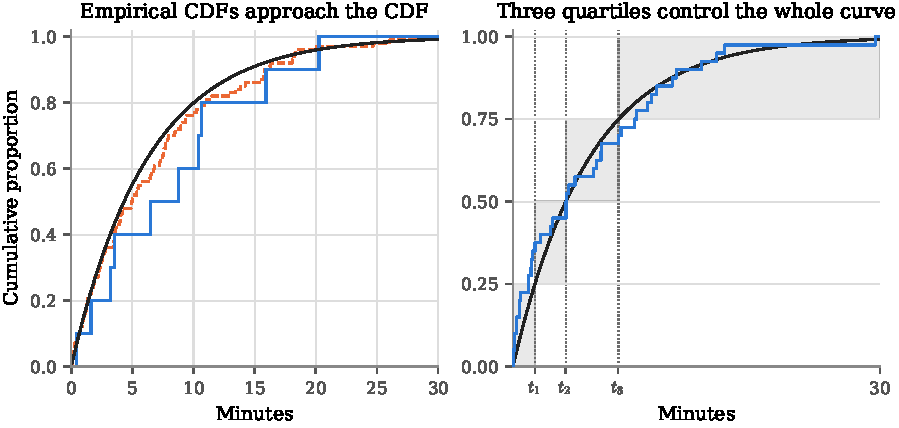
\includegraphics[width=\textwidth]{fig_ecdf_gc}
\caption{Simulated waits, mean $6.23$; the exponential CDF (black) in both halves. Left: empirical CDFs for $n = 10$ (blue) and $n = 100$ (orange, dashed). Right: quartiles $t_1, t_2, t_3$ (dotted), four gray boxes, and an empirical CDF for $n = 40$ (blue).}
\label{fig:ecdfgc}
\end{figure}

The largest gap is itself a distance between distributions, the \textbf{Kolmogorov distance} $\sup_t\abs{F(t) - G(t)}$ between the distributions with CDFs $F$ and $G$.
It compares the probabilities of the half-lines $(-\infty, t]$ only, where total variation compares those of all events, so it is never larger than the total variation distance (\cref{ex:ks-tv}).
That restriction is what makes it estimable.
\Cref{sec:dist-tv-estimate} showed that the empirical distribution of continuous data sits at total variation $1$ from the truth at every $n$; at Kolmogorov distance it converges to the truth, by the Glivenko--Cantelli theorem.
For the exponential $\Expo(1)$ and $\Gauss(1, 1)$, its closest Gaussian in KL divergence (\cref{ch:distances}), the Kolmogorov distance is $0.159$, attained at $0$, below which the Gaussian puts probability $\Phi(-1) = 0.159$ and the exponential none; their total variation distance is $0.319$.

How fast does the largest gap shrink?
In $4{,}000$ simulated samples its median is $0.247$ at $n = 10$, $0.081$ at $n = 100$ and $0.026$ at $n = 1{,}000$, and $\sqrt{n}$ times the median is close to $0.8$ at all three.
The gap shrinks like $1/\sqrt{n}$, as the error of an average does, and the next section finds the distribution of $\sqrt{n}$ times it.

\section{The size of the gap: Donsker's theorem}
\label{sec:ks-donsker}

Multiplying by $\sqrt{n}$, as the CLT does for an average, turns the gap into a random curve, $t \mapsto \sqrt{n}(F_n(t) - F(t))$.
By \cref{prop:ecdf-pointwise}, at each $t$ it is approximately $\Gauss(0, F(t)(1 - F(t)))$, and its values at two points $s \leq t$ have covariance $F(s)(1 - F(t))$.
The variance is largest where $F = \frac12$ and falls to $0$ at both ends, where $F_n$ and $F$ are both pinned near $0$ or near $1$.
For uniform data, $F(u) = u$ on $[0, 1]$, the curve is $u \mapsto \sqrt{n}(G_n(u) - u)$, with $G_n$ the empirical CDF of $n$ independent $\Unif(0, 1)$ draws $U_1, \ldots, U_n$, and the covariance at $u \leq v$ is $u(1 - v) = \min(u, v) - uv$.

\recall{The Central Limit Theorem for vectors (the vector-versions remark of \cref{ch:limit-tools}): for i.i.d.\ random vectors $Y_i$ with mean $m$ and positive definite covariance matrix $\Sigma$, $\sqrt{n}(\bar{Y}_n - m) \convd \Gauss_d(0, \Sigma)$.}

At finitely many points $u_1 < \cdots < u_k$ in $(0, 1)$, the values of this curve are $\sqrt{n}$ times the centered average of the i.i.d.\ vectors $(\ind(U_i \leq u_1), \ldots, \ind(U_i \leq u_k))$, and the CLT for vectors makes them jointly Gaussian in the limit (the covariance matrix is positive definite; \cref{ex:ks-cov} checks two points).
The limit of the whole curve is a random function with those Gaussian values.

\begin{theorem}[Kolmogorov; Donsker]
\label{thm:donsker}
Let $\Xton$ be i.i.d.\ with a continuous CDF $F$. Then
\[
\sqrt{n}\,\sup_{t \in \real}\abs{F_n(t) - F(t)} \convd K,
\]
where $K$ is the largest absolute value of a \textbf{Brownian bridge}: a random continuous function $B$ on $[0, 1]$ with $B(0) = B(1) = 0$ whose values at any points $0 < u_1 < \cdots < u_k < 1$ form a Gaussian vector with mean $0$ and $\cov(B(u), B(v)) = \min(u, v) - uv$. The distribution of $K$, \textbf{Kolmogorov's distribution}, is
\[
\Pr(K > x) = 2\sum_{j=1}^\infty (-1)^{j-1}e^{-2j^2x^2}, \qquad x > 0,
\]
and its $95\%$ quantile is $q_{0.05}(K) = 1.358$ ($1.224$ for $90\%$, $1.628$ for $99\%$).
\end{theorem}

This theorem is stated without proof.
The part about finitely many points follows from the CLT for vectors, as above; the step from finitely many points to the largest gap over all of them needs a theory of convergence for random functions that this book does not develop.
Donsker's theorem proper says that the whole curve $u \mapsto \sqrt{n}(G_n(u) - u)$ converges in distribution to $B$; this book uses only its consequence for the largest gap.
Kolmogorov (\textit{Giornale dell'Istituto Italiano degli Attuari}, 1933) found the limit distribution, and Smirnov (\textit{Annals of Mathematical Statistics}, 1948) tabulated it; Doob (\textit{Annals of Mathematical Statistics}, 1949) saw, and Donsker (\textit{Annals of Mathematical Statistics}, 1952) proved, that it is the distribution of the largest absolute value of the limiting curve, the Brownian bridge.
Notice what the limit does not depend on: $F$.
Every continuous distribution leads to the same $K$, which the next section explains.

The left of \cref{fig:brownianbridge} shows four curves $\sqrt{n}(G_n(u) - u)$ for $n = 1{,}000$ uniform draws.
They already look like the limit: pinned to $0$ at both ends, wandering most in the middle, and, like about $19$ in $20$ such curves, staying inside $\pm 1.358$.
The right compares the distribution of $\sqrt{n}$ times the largest gap at $n = 100$ with Kolmogorov's density; at $n = 100$ the exact $95\%$ point is $1.340$, against the limit's $1.358$.

\begin{figure}[htbp]
\centering
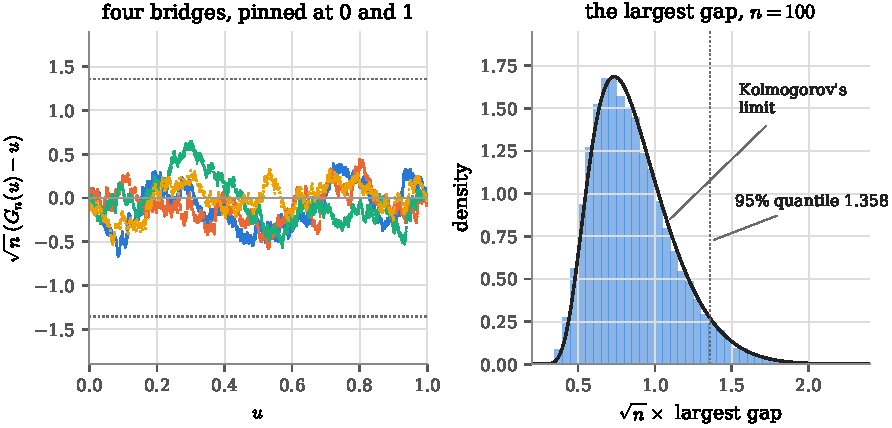
\includegraphics[width=\textwidth]{fig_brownian_bridge}
\caption{Uniform data. Left: four curves $\sqrt{n}(G_n(u) - u)$ for $n = 1{,}000$, and $\pm 1.358$ (dotted). Right: $\sqrt{n}$ times the largest gap in $20{,}000$ samples of $n = 100$ (histogram), Kolmogorov's density (black) and its $95\%$ quantile (dotted).}
\label{fig:brownianbridge}
\end{figure}

\begin{sanitycheck}[Why is the threshold 1.36 and not 0.98?]
At the single point $u = \frac12$ the bridge has variance $\frac12 - \frac14 = \frac14$, so $\abs{B(\frac12)}$ exceeds $1.96 \times \frac12 = 0.98$ with probability $5\%$.
$K$ is the largest $\abs{B(u)}$ over the whole curve, so it exceeds $0.98$ more often, and its $95\%$ point must be higher.
It is $1.358$, which is the $95\%$ point of the largest of about eight independent values distributed like $\abs{B(\frac12)}$: values of the bridge at nearby points move together, so infinitely many points behave like a handful.
The same contrast set the thresholds of the multiple-testing corrections of \cref{sec:t-multiple}: the largest of many statistics needs a larger threshold than any one of them.
\end{sanitycheck}

\textbf{A confidence band.}
For continuous $F$, since $\Pr(\sqrt{n}\sup_t\abs{F_n(t) - F(t)} \leq 1.358) \to 0.95$, the band $F_n(t) \pm 1.358/\sqrt{n}$ contains the entire curve $F$ with probability tending to $95\%$.
For Old Faithful, $n = 272$ and the half-width is $1.358/\sqrt{272} = 0.082$, so at $60$ minutes the band is $[0.223, 0.387]$, wider than the pointwise interval $[0.250, 0.360]$ of \cref{sec:ks-ecdf}, since the band must cover every $t$ at once.
The band does not even need large $n$.
Massart (\textit{Annals of Probability}, 1990) proved the Dvoretzky--Kiefer--Wolfowitz inequality with its best constant: for every $n$, every $\varepsilon > 0$ and every $F$,
\[
\Pr\Big(\sup_t\abs{F_n(t) - F(t)} > \varepsilon\Big) \leq 2e^{-2n\varepsilon^2}.
\]
Setting the right side to $0.05$ gives $\varepsilon = \sqrt{\log 40/(2n)} = 1.3581/\sqrt{n}$, the asymptotic half-width to four digits, so the band with this half-width covers $F$ with probability at least $95\%$ at every $n$, whatever $F$ is.
(The inequality is stated without proof; nothing later depends on it.)
A band tests every candidate at once: a stated CDF is rejected at the $5\%$ level when it leaves the band somewhere, and a family is rejected when every member does.
The Gaussian CDF closest to the Old Faithful staircase in Kolmogorov distance has mean $72.5$ and standard deviation $15.1$ and is $0.102$ away, outside the band, so no Gaussian fits the waits.

\section{The Kolmogorov--Smirnov test}
\label{sec:ks-test}

To test whether data come from a stated continuous distribution, measure the largest gap between its CDF and the empirical CDF.
The alternative is every other distribution, which no finite list of parameters describes; over all densities the likelihood has no maximum (a density can be made as tall as we like at the observed points), so the tests of \cref{ch:wald-lrt} do not apply, and the statistic is built from the empirical CDF alone.

\begin{definition}[The Kolmogorov--Smirnov test]
\label{def:ks-test}
Let $F^0$ be a continuous CDF. For $H_0: F = F^0$ against $H_1: F \neq F^0$, the \textbf{Kolmogorov--Smirnov statistic} is
\[
D_n = \sup_{t \in \real}\abs{F_n(t) - F^0(t)},
\]
and the \textbf{Kolmogorov--Smirnov test} of level $\alpha$ rejects when $D_n > d_\alpha(n)$, the $1 - \alpha$ quantile of $D_n$ under $H_0$. The test of asymptotic level $\alpha$ rejects when $\sqrt{n}D_n > q_\alpha(K)$, which is $1.358$ for $\alpha = 0.05$.
\end{definition}

\begin{inwords}
\textbf{In words.} Draw the candidate CDF and the staircase of the data on the same axes, find the largest vertical distance between them, and reject when it is larger than chance alone would make it. The threshold shrinks like $1/\sqrt{n}$: about $1.36/\sqrt{n}$ at the $5\%$ level.
\par\smallskip
\textbf{For the kiss data.} The kiss data are $0$s and $1$s, and the candidate $p = \frac12$ has a two-step CDF, so $D_n = \abs{F_n(0) - F^0(0)} = \abs{0.355 - 0.5} = 0.145$, the gap in the proportion of left turns, and $\sqrt{124}\,D_n = 1.62$, half the statistic $3.23$ of \cref{ch:tests-foundations}. But $F^0$ is not continuous, and the theory below does not apply: with this discrete null the threshold $1.358$ would reject a true null about $5$ times in $1{,}000$ at $n = 124$ ($0.66\%$ in the limit), not $50$ times (\cref{ex:ks-discrete}). Discrete data belong to the tests of \cref{ch:tests-foundations,ch:gof}.
\end{inwords}

The supremum runs over infinitely many $t$, but only $2n$ numbers need checking.

\begin{proposition}[Computing the statistic]
\label{prop:ks-compute}
If $F^0$ is continuous,
\[
D_n = \max_{1 \leq i \leq n}\max\Big(\frac{i}{n} - F^0(X_{(i)}),\ F^0(X_{(i)}) - \frac{i - 1}{n}\Big).
\]
\end{proposition}

\optionalproof{Between two observations the staircase is flat and $F^0$ only rises, so the largest gaps sit at the steps.}
\begin{proof}
On $[X_{(i)}, X_{(i+1)})$, $F_n = i/n$ and $F^0$ is nondecreasing, so $F_n - F^0$ is largest at the left end, where it is $i/n - F^0(X_{(i)})$, and $F^0 - F_n$ approaches its supremum $F^0(X_{(i+1)}) - i/n$ at the right end, by the continuity of $F^0$.
On $(-\infty, X_{(1)})$, $F_n = 0$ and the gap $F^0(t)$ approaches $F^0(X_{(1)}) - 0$; on $[X_{(n)}, \infty)$, $F_n = 1$ and the gap $1 - F^0(t)$ is largest at $X_{(n)}$, where it is $n/n - F^0(X_{(n)})$.
These are the $2n$ terms of the formula.
If several observations are tied, $X_{(i)} = \cdots = X_{(j)}$, the staircase jumps from $(i - 1)/n$ to $j/n$ there; the terms $j/n - F^0(X_{(j)})$ and $F^0(X_{(i)}) - (i - 1)/n$ are the gaps at that value and just below it, and the other terms of the block are no larger.
\end{proof}

\begin{worked}[ten random numbers]
A random number generator should produce independent $\Unif(0, 1)$ values.
Ten of its outputs, sorted and rounded to two decimals, are in the second row below. Here $F^0(u) = u$, so the two terms of \cref{prop:ks-compute} are the last two rows:
\begin{center}
\small
\begin{tabular}{@{}lrrrrrrrrrr@{}}
\toprule
$i$ & $1$ & $2$ & $3$ & $4$ & $5$ & $6$ & $7$ & $8$ & $9$ & $10$ \\
\midrule
$u_{(i)}$ & $0.08$ & $0.17$ & $0.38$ & $0.51$ & $0.54$ & $0.61$ & $0.80$ & $0.87$ & $0.94$ & $0.98$ \\
$i/10 - u_{(i)}$ & $0.02$ & $0.03$ & $-0.08$ & $-0.11$ & $-0.04$ & $-0.01$ & $-0.10$ & $-0.07$ & $-0.04$ & $0.02$ \\
$u_{(i)} - (i-1)/10$ & $0.08$ & $0.07$ & $0.18$ & $0.21$ & $0.14$ & $0.11$ & $0.20$ & $0.17$ & $0.14$ & $0.08$ \\
\bottomrule
\end{tabular}
\end{center}
The largest entry is $0.51 - 0.30 = 0.21$: just below $0.51$ the staircase is still at $0.30$, while the uniform CDF has reached $0.51$.
So $D_{10} = 0.21$.
The exact $5\%$ threshold for $n = 10$ is $d_{0.05}(10) = 0.409$, and the exact $p$-value is $\Pr(D_{10} \geq 0.21) = 0.70$: nothing here suggests that the generator is broken.
The asymptotic version agrees: $\sqrt{10} \times 0.21 = 0.664 < 1.358$, with $p$-value $\Pr(K > 0.664) = 0.77$.
The left of \cref{fig:ksexample} draws the staircase, the uniform CDF and this largest gap, in orange.
\end{worked}

The worked example used the uniform candidate, and nothing in it was special to the uniform.

\begin{lemma}[The probability integral transform]
\label{lem:pit}
If $X$ has a continuous CDF $F$, then $F(X) \sim \Unif(0, 1)$.
\end{lemma}

\coreproof{The event $F(X) \leq u$ is the event that $X$ is at or below the last point where $F$ equals $u$, and that has probability $u$.}
\begin{proof}
Fix $u \in (0, 1)$.
Since $F$ is continuous and runs from $0$ to $1$, it takes the value $u$ (the intermediate value theorem), and since it is nondecreasing and continuous, the set where $F(t) = u$ is a closed, bounded interval $[a, b]$, possibly a single point.
If $X \leq b$ then $F(X) \leq F(b) = u$; if $X > b$ then $F(X) > u$, since $b$ is the last point where $F$ equals $u$.
So $\Pr(F(X) \leq u) = \Pr(X \leq b) = F(b) = u$, which is the CDF of $\Unif(0, 1)$.
\end{proof}

\begin{theorem}[The Kolmogorov--Smirnov test]
\label{thm:ks}
Let $\Xton$ be i.i.d.\ with CDF $F$, and let $F^0$ be continuous.
\begin{enumerate}[nosep]
\item If $F = F^0$, then $D_n$ has the distribution of $\sup_{0 \leq u \leq 1}\abs{G_n(u) - u}$, where $G_n$ is the empirical CDF of $n$ i.i.d.\ $\Unif(0, 1)$ variables. It is the same for every continuous $F^0$, so the test of \cref{def:ks-test} has level $\alpha$, and by \cref{thm:donsker} the test with threshold $q_\alpha(K)/\sqrt{n}$ has asymptotic level $\alpha$.
\item If $F \neq F^0$, then $D_n \convp \sup_t\abs{F(t) - F^0(t)} > 0$, and the probability that either test rejects tends to $1$.
\end{enumerate}
\end{theorem}

\coreproof{Push every observation through $F^0$. Under $H_0$ the transformed values are uniform, and the vertical gaps between the staircase and the candidate do not change, since the transformation only moves points along the horizontal axis.}
\begin{proof}
(1) Suppose first that $F^0$ is strictly increasing on the interval where $0 < F^0 < 1$.
Let $U_i = F^0(X_i)$; under $H_0$ these are i.i.d.\ $\Unif(0, 1)$ by \cref{lem:pit}, and with probability $1$ every $X_i$ lies in that interval.
For such an $X_i$ and every $t$, $X_i \leq t$ exactly when $U_i \leq F^0(t)$, so $F_n(t) = G_n(F^0(t))$, where $G_n$ is the empirical CDF of $U_1, \ldots, U_n$.
Hence
\[
D_n = \sup_t\abs{G_n(F^0(t)) - F^0(t)} = \sup_{0 < u < 1}\abs{G_n(u) - u},
\]
since $F^0(t)$ takes every value in $(0, 1)$ as $t$ runs over the line; at $u = 0$ and $u = 1$ the gap is $0$ with probability $1$.
If $F^0$ is flat on a stretch, extend the stretch as far as $F^0$ stays flat: the result is a closed stretch of probability $0$.
There are at most countably many of these longest flat stretches (they do not overlap and each has positive length, so each contains a rational number of its own), so with probability $1$ no observation falls in one, endpoints included.
For every other value of $X_i$ the equivalence above still holds: if $X_i > t$ and $F^0(X_i) = F^0(t)$, then $F^0$ is flat on $[t, X_i]$, a stretch containing $X_i$.
The threshold $d_\alpha(n)$ is a quantile of this one distribution, which gives the level; and the uniform distribution is continuous, so \cref{thm:donsker} applied to $U_1, \ldots, U_n$ gives the asymptotic level.

(2) By the triangle inequality, at every $t$, $\abs{F_n(t) - F^0(t)}$ differs from $\abs{F(t) - F^0(t)}$ by at most $\abs{F_n(t) - F(t)}$, so $D_n$ differs from $c = \sup_t\abs{F(t) - F^0(t)}$ by at most $\sup_t\abs{F_n(t) - F(t)}$, which converges to $0$ in probability by \cref{thm:glivenko-cantelli}.
Hence $D_n \convp c$, and $c > 0$ since $F \neq F^0$.
Both thresholds tend to $0$: $q_\alpha(K)/\sqrt{n}$ plainly, and $d_\alpha(n)$ since, under $H_0$, the Glivenko--Cantelli theorem gives $\Pr(D_n > \varepsilon) < \alpha$ for large $n$ and any $\varepsilon > 0$, so that $d_\alpha(n) \leq \varepsilon$.
Once both thresholds are below $c/2$, the probability of rejecting is at least $\Pr(D_n > c/2)$, which tends to $1$.
\end{proof}

\begin{intuition}[one table for every continuous distribution]
The right of \cref{fig:ksexample} takes the ten generator outputs of the worked example and sends each through the exponential quantile function, $x = -5\log(1 - u)$, which turns uniform numbers into exponential waits with mean $5$ minutes (\cref{ex:ks-pit}).
Against the exponential CDF the new staircase has the same steps at the same heights, and every gap is the same, including $D_{10} = 0.21$.
That is the theorem: an increasing transformation stretches the horizontal axis and leaves heights alone, and the Kolmogorov--Smirnov statistic measures only heights.
So the null distribution of $D_n$ can be computed once, for uniform data, and used for every continuous $F^0$.
Massey (\textit{Journal of the American Statistical Association}, 1951) published such a table, for $n$ up to $35$, and a simulation of uniform samples reproduces any entry of it.
\end{intuition}

\begin{figure}[htbp]
\centering
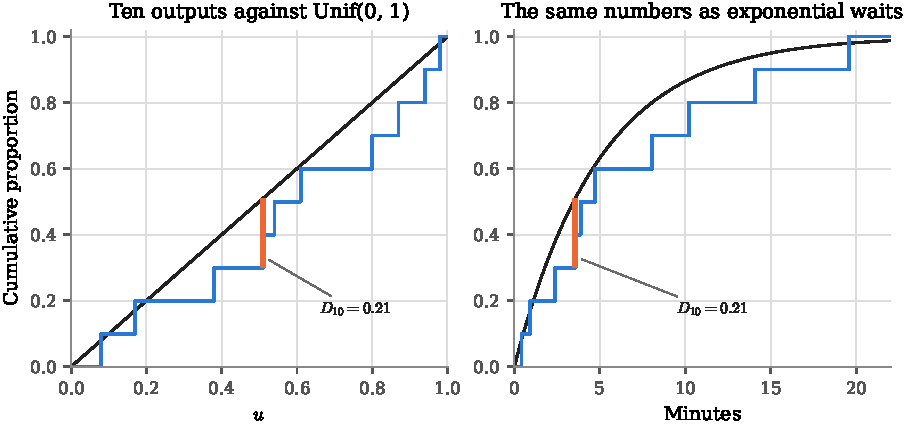
\includegraphics[width=\textwidth]{fig_ks_example}
\caption{Left: the empirical CDF (blue) of ten generator outputs against the $\Unif(0, 1)$ CDF (black), largest gap in orange. Right: the same values as exponential waits, $x = -5\log(1 - u)$, against the exponential CDF with mean $5$.}
\label{fig:ksexample}
\end{figure}

The exact thresholds approach $1.358/\sqrt{n}$ from below: for $n = 5$, $10$, $20$, $50$ and $100$ they are $0.563$, $0.409$, $0.294$, $0.188$ and $0.134$, against $0.607$, $0.429$, $0.304$, $0.192$ and $0.136$.
So the asymptotic test is slightly conservative, and from $n = 50$ on the two thresholds agree to within about $2\%$.

\section{Other measures of the gap}
\label{sec:ks-other}

The Kolmogorov--Smirnov statistic keeps only the largest gap.
Two other classical statistics add up the squared gaps over the whole line, weighting each $t$ by the probability the candidate puts near it:
\[
W^2_n = n\int_{-\infty}^\infty \big(F_n(t) - F^0(t)\big)^2 f^0(t)\,\mathrm{d}t, \qquad
A^2_n = n\int_{-\infty}^\infty \frac{\big(F_n(t) - F^0(t)\big)^2}{F^0(t)\big(1 - F^0(t)\big)}\, f^0(t)\,\mathrm{d}t,
\]
the \textbf{Cram\'er--von Mises} and \textbf{Anderson--Darling} statistics, with $f^0$ the density of $F^0$ (Anderson and Darling, \textit{Annals of Mathematical Statistics}, 1952, introduced the second).
The substitution $u = F^0(t)$, with $\mathrm{d}u = f^0(t)\,\mathrm{d}t$, turns both into integrals over $[0, 1]$ of the uniform staircase $G_n$ of \cref{thm:ks}, so both are distribution-free in the same way.
With $U_{(i)} = F^0(X_{(i)})$ they are computed as
\[
W^2_n = \frac{1}{12n} + \sum_{i=1}^n\Big(U_{(i)} - \frac{2i - 1}{2n}\Big)^2, \qquad
A^2_n = -n - \frac1n\sum_{i=1}^n(2i - 1)\Big(\log U_{(i)} + \log\big(1 - U_{(n+1-i)}\big)\Big)
\]
(\cref{ex:ks-cvm} derives the first), and their $5\%$ thresholds are about $0.46$ and $2.49$ for large $n$.

The weight in $A^2_n$ has a reason.
The gap at $t$ has variance $F(t)(1 - F(t))/n$ (\cref{prop:ecdf-pointwise}), which falls to $0$ in the tails.
The Kolmogorov--Smirnov statistic and $W^2_n$ measure raw gaps, which are naturally small in the tails, so they hardly look there.
$A^2_n$ divides each squared gap by its variance, as Pearson's statistic divided each squared deviation by its expected count in \cref{ch:gof}, and a gap in the tails then counts as much as one in the middle.

\Cref{fig:edfpower} puts the three ideas side by side for a Gaussian null with $n = 50$: the Kolmogorov--Smirnov test, the Anderson--Darling test, and Pearson's test on the counts in $4$ or in $10$ cells equally likely under the null, each with level $5\%$ or just below, its threshold simulated under the null.
When the mean is off by $0.4$ standard deviations they reject $69\%$, $78\%$, $57\%$ and $42\%$ of the time.
Binning gives something up: each observation becomes the name of its cell, and with more cells each count is noisier.
When the spread is $1.5$ times too large the order changes: $36\%$, $81\%$, $40\%$ and $60\%$.
A change of spread moves the tails most, where the Kolmogorov--Smirnov statistic hardly looks, and when the spread is $0.7$ times what it should be, the two binned tests ($47\%$ and $42\%$) beat both of the others ($17\%$ and $26\%$).
No test wins everywhere; the Anderson--Darling test loses least across these alternatives.

\begin{figure}[htbp]
\centering
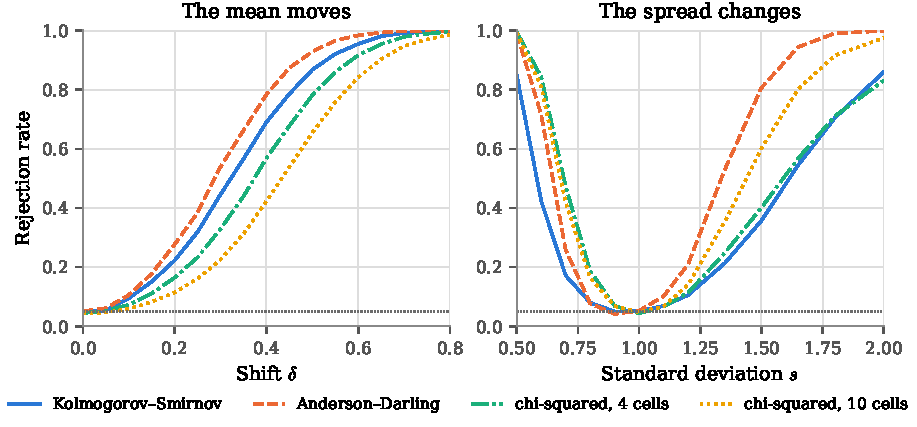
\includegraphics[width=\textwidth]{fig_edf_power}
\caption{Rejection rates of four $5\%$ tests of $\Gauss(0, 1)$ with $n = 50$: Kolmogorov--Smirnov, Anderson--Darling, and Pearson's test on $4$ or $10$ equally likely cells. Left: data from $\Gauss(\delta, 1)$. Right: data from $\Gauss(0, s^2)$. Gray dotted line: $5\%$.}
\label{fig:edfpower}
\end{figure}

\section{Testing a family: the Lilliefors test}
\label{sec:ks-lilliefors}

The question asked of data is rarely `is this $\Gauss(0, 1)$?' and usually `is this Gaussian?', with the mean and variance unknown; before the $t$-test of \cref{ch:t-test}, for instance.
The obvious move is to plug in estimates,
\[
\hat{D}_n = \sup_t\abs{F_n(t) - \Phi\Big(\frac{t - \bar{X}_n}{S_n}\Big)},
\]
with $\bar{X}_n$ and $S_n$ the sample mean and standard deviation (with divisor $n - 1$, as in \cref{ch:t-test}; the thresholds below use it), and to compare $\hat{D}_n$ with the Kolmogorov--Smirnov threshold.

\begin{pitfall}[the Kolmogorov--Smirnov table with estimated parameters]
The fitted Gaussian is chosen to match the data, so it sits closer to the empirical CDF than the true Gaussian does, and $\hat{D}_n$ is systematically smaller than $D_n$.
The left of \cref{fig:lilliefors} shows the two null distributions for $n = 50$: $95\%$ of the time $\sqrt{n}\hat{D}_n$ is below $0.88$, while the Kolmogorov--Smirnov threshold is $1.33$.
Using that threshold for $\hat{D}_n$ gives a test that rejects a true Gaussian model fewer than $2$ times in $10{,}000$ samples, at $n = 50$ and at $n = 100$ alike, where it should reject $500$ times.
\Cref{ch:gof} met the same effect for the chi-squared test: a parameter fitted to the data makes the fit look better than it is, which there cost a degree of freedom for each parameter fitted from the counts, and left no exact correction when the parameters came from the raw data (a Gaussian in four cells, compared with $\chi^2_1$ instead of $\chi^2_3$, rejected $10.5\%$ of the time in the limit instead of $5\%$: the correction overshot). For the Kolmogorov--Smirnov statistic the effect is larger, and no change of degrees of freedom repairs it.
\end{pitfall}

The repair is to find the null distribution of $\hat{D}_n$ itself, and it can be found once and for all.

\begin{proposition}[The fitted statistic is pivotal]
\label{prop:lilliefors}
Let $\Xton \iid \Gauss(\mu, \sigma^2)$, $n \geq 2$. The distribution of $\hat{D}_n$ does not depend on $\mu$ or $\sigma^2$: it is the distribution of the same statistic computed from $n$ i.i.d.\ standard Gaussians.
\end{proposition}

\coreproof{Standardize the data. Shifting and rescaling a sample shifts and rescales its empirical CDF, its mean and its standard deviation together, so every gap stays where it was.}
\begin{proof}
Write $X_i = \mu + \sigma Z_i$ with $Z_1, \ldots, Z_n \iid \Gauss(0, 1)$, and let $\bar{Z}_n$, $S^Z_n$ and $F^Z_n$ be the mean, standard deviation and empirical CDF of the $Z_i$.
Then $\bar{X}_n = \mu + \sigma\bar{Z}_n$ and $S_n = \sigma S^Z_n$.
For every $t$, put $s = (t - \mu)/\sigma$: $X_i \leq t$ exactly when $Z_i \leq s$, so $F_n(t) = F^Z_n(s)$, and $(t - \bar{X}_n)/S_n = (s - \bar{Z}_n)/S^Z_n$.
As $t$ runs over the line so does $s$, so
\[
\hat{D}_n = \sup_s\abs{F^Z_n(s) - \Phi\Big(\frac{s - \bar{Z}_n}{S^Z_n}\Big)},
\]
a function of $Z_1, \ldots, Z_n$ alone.
\end{proof}

\begin{definition}[The Lilliefors test for normality]
\label{def:lilliefors}
For $H_0$: the $X_i$ are i.i.d.\ $\Gauss(\mu, \sigma^2)$ for some $\mu$ and some $\sigma^2 > 0$, against $H_1$: they are not, the \textbf{Lilliefors test} of level $\alpha$ rejects when $\hat{D}_n > \ell_\alpha(n)$, the $1 - \alpha$ quantile of $\hat{D}_n$ under $H_0$, computed by simulating samples of $n$ standard Gaussians (\cref{prop:lilliefors}).
\end{definition}

\begin{inwords}
\textbf{In words.} Fit the Gaussian with the sample mean and standard deviation, measure the largest gap as before, and compare it with a threshold made for fitted Gaussians, about two thirds of the Kolmogorov--Smirnov one.
\par\smallskip
\textbf{For the kiss data.} The Gaussian with the kiss data's mean $0.645$ and standard deviation $0.480$ gives $\hat{D}_{124} = 0.415$, attained just below $1$, where the staircase is at $0.355$ and the fitted Gaussian at $0.770$; the $5\%$ threshold for $n = 124$ is $0.080$. Two-valued data are far from Gaussian, which is why the $t$-test of \cref{ch:t-test} is only asymptotically valid for them.
\end{inwords}

\begin{center}
\small
\begin{tabular}{@{}lrrrrr@{}}
\toprule
$n$ & $5$ & $10$ & $20$ & $50$ & $100$ \\
\midrule
Kolmogorov--Smirnov, $d_{0.05}(n)$ & $0.563$ & $0.409$ & $0.294$ & $0.188$ & $0.134$ \\
Lilliefors, $\ell_{0.05}(n)$ & $0.343$ & $0.262$ & $0.192$ & $0.125$ & $0.089$ \\
\bottomrule
\end{tabular}
\end{center}

The table gives $5\%$ thresholds for both tests; the Lilliefors values come from $200{,}000$ simulated samples for each $n$, and for large $n$ they are about $0.9/\sqrt{n}$, against $1.36/\sqrt{n}$.
Lilliefors (\textit{Journal of the American Statistical Association}, 1967) made the first such table by simulation.
The proof of \cref{prop:lilliefors} works for any family obtained by shifting and rescaling one distribution, with estimates that shift and rescale along with the data, and also for the exponential scale family (\cref{ex:ks-expo}).
For families without this invariance the null distribution depends on the true parameter, and simulating samples from the fitted distribution is the usual approximation.

\begin{worked}[Newcomb's measurements of the speed of light]
In 1882 Simon Newcomb measured, $66$ times, the time light takes to travel to a distant mirror and back, a known distance of about $7.4$ kilometers; the values are in nanoseconds above $24{,}800$ (Stigler, \textit{Annals of Statistics}, 1977).
Sixty-four of them lie between $16$ and $40$; the other two are $-44$ and $-2$.
All $66$ have mean $26.2$ and standard deviation $10.7$, and the fitted Gaussian is $\hat{D}_{66} = 0.231$ from the staircase, against the $5\%$ threshold $\ell_{0.05}(66) = 0.109$: none of $40{,}000$ simulated Gaussian samples came this far, and the test rejects.
Without the two low values, the $64$ that remain have mean $27.75$ and standard deviation $5.08$, and $\hat{D}_{64} = 0.090$ is below the threshold $\ell_{0.05}(64) = 0.111$: no evidence against a Gaussian shape.
The two values that sink the test stand out at once in the QQ plot of \cref{sec:ks-qq}.
The modern value of the speed of light corresponds to $33.0$ in these units, so the $64$ good measurements also share a systematic error of about $5$, which no test of shape can see.
\end{worked}

The right of \cref{fig:lilliefors} is the Old Faithful staircase against its fitted Gaussian, with mean $70.9$ and standard deviation $13.6$.
The fitted Gaussian puts probability $0.62$ below $75$ minutes, while only $46\%$ of the observed waits are that short; the gap, $\hat{D}_{272} = 0.155$, is almost three times the threshold $\ell_{0.05}(272) = 0.054$, and none of $20{,}000$ simulated samples came this far.
The waits are a mixture of two kinds of eruption (\cref{fig:emfaithful}), and a single Gaussian is the wrong shape.

\textbf{Rounded data.}
Newcomb's values are whole numbers and the waits are whole minutes, so both samples contain ties.
\Cref{prop:ks-compute} still computes the statistic, but rounding alone makes the staircase take bigger steps, which moves the null distribution of $\hat{D}_n$ up; the thresholds above are for unrounded data.
Gaussian samples with the fitted mean and standard deviation, rounded the same way, give $5\%$ thresholds of $0.116$ for Newcomb's $66$ values, $0.131$ for his $64$ good ones, where the $p$-value of $\hat{D}_{64} = 0.090$ rises from $0.21$ to $0.56$, and $0.063$ for the $272$ waits.
The two low values still sink Newcomb's test, the other $64$ still pass, and Old Faithful's $0.155$ is still far above its threshold.

\begin{figure}[htbp]
\centering
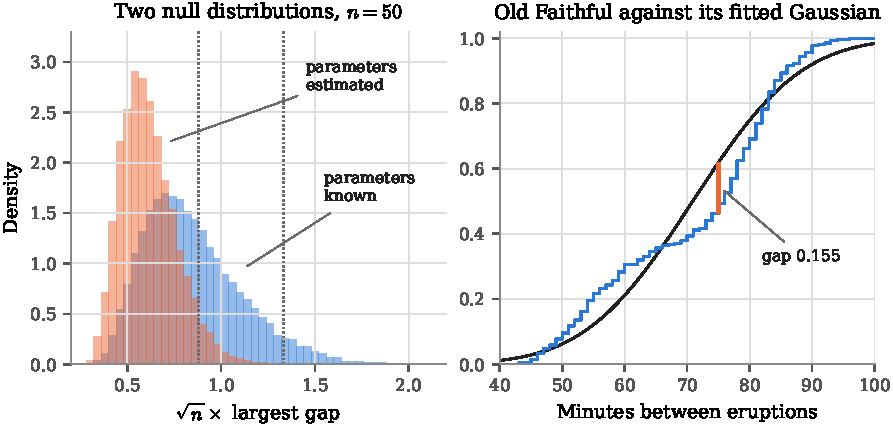
\includegraphics[width=\textwidth]{fig_lilliefors}
\caption{Left: for $n = 50$, $\sqrt{n}$ times the largest gap to the true Gaussian (blue) and the fitted one (orange); $95\%$ points $1.33$ and $0.88$ dotted. Right: Old Faithful's waits (blue), fitted Gaussian (black), largest gap (orange).}
\label{fig:lilliefors}
\end{figure}

Not rejecting is weak evidence when the sample is small.
With $12$ observations, the size of the wind-turbine sample of \cref{ch:t-test}, the Lilliefors test detects exponential data only $36\%$ of the time and data from Student's $t$ with $3$ degrees of freedom $18\%$ of the time; with $20$ observations, $58\%$ and $26\%$.

\begin{bridge}[checking normality before a $t$-test]
An introductory course asks for a look at a histogram, or a normal probability plot, before a $t$-test on a small sample, and software often reports a formal test of normality, commonly the Shapiro--Wilk test, which is more powerful than Lilliefors' against many alternatives.
The Lilliefors test is the formal version of the histogram check, and the QQ plot of the next section is the normal probability plot.
Formal tests are limited the way \cref{ch:gof} found: a small sample shows little, as the $36\%$ above says, and a large sample finds every departure, including ones that do not matter for a $t$-test, whose level the CLT protects at large $n$ (\cref{ch:t-test}).
\end{bridge}

\section{QQ plots}
\label{sec:ks-qq}

A test answers yes or no.
A QQ plot shows where the data depart from a candidate, and how.
It compares quantiles instead of CDF heights: the $i$th smallest observation $X_{(i)}$ is a sample quantile of order about $i/n$, and if the data come from $F$ it should be close to the population quantile of the same order.

\begin{definition}[QQ plot]
\label{def:qq}
Let $F$ be a continuous CDF, strictly increasing where $0 < F < 1$, with quantile function $F^{-1}$ (\cref{ch:gaussian}). The \textbf{QQ plot} of a sample against $F$ is the set of points
\[
\Big(F^{-1}\Big(\frac{i - 1/2}{n}\Big),\ X_{(i)}\Big), \qquad i = 1, \ldots, n.
\]
Against $F = \Phi$, the standard Gaussian CDF, it is called a \textbf{normal QQ plot}.
\end{definition}

\begin{inwords}
\textbf{In words.} Sort the data, and pair the $i$th smallest value with the point below which the candidate puts a fraction $(i - \frac12)/n$ of its probability. Some authors use $i/n$ and drop the last point, whose quantile $F^{-1}(1)$ is infinite; the picture is the same.
\par\smallskip
\textbf{For the kiss data.} Against Gaussian quantiles the kiss data plot as two flat rows, $44$ points at height $0$ and $80$ at height $1$. A two-valued sample gives a staircase, never a line.
\end{inwords}

If $X \sim \Gauss(\mu, \sigma^2)$, its quantile of order $p$ is $\mu + \sigma\Phi^{-1}(p)$, so the normal QQ plot of Gaussian data lies near a straight line with slope $\sigma$ and height $\mu$ at $0$, whatever $\mu$ and $\sigma$ are.
That is why one normal QQ plot checks the whole Gaussian family: the question is whether the points lie on some line, not on a particular one.
The figures below draw the line through the points at the first and third quartiles, which outliers cannot pull.

\begin{intuition}[reading the ends of a QQ plot]
For data with a single peak, the middle of a QQ plot is usually close to straight, and the ends carry the information.
\Cref{fig:qqpatterns} shows four samples of $200$ against Gaussian quantiles.
Heavy tails, as for Student's $t$ with $3$ degrees of freedom: the smallest values are smaller and the largest larger than a Gaussian with the same quartiles would give, so the left end falls below the line and the right end rises above it.
Light tails, as for the uniform: the opposite, with both ends bending back toward the horizontal.
Skewed right, as for the exponential: the lower tail is short and the upper tail long, so the points bend upward, above the line at both ends and below it in the middle.
Skewed left: the mirror image, bending down.
The skewed-right plot is the picture \cref{ch:distances} promised for exponential data and their closest Gaussian.
\end{intuition}

\begin{figure}[htbp]
\centering
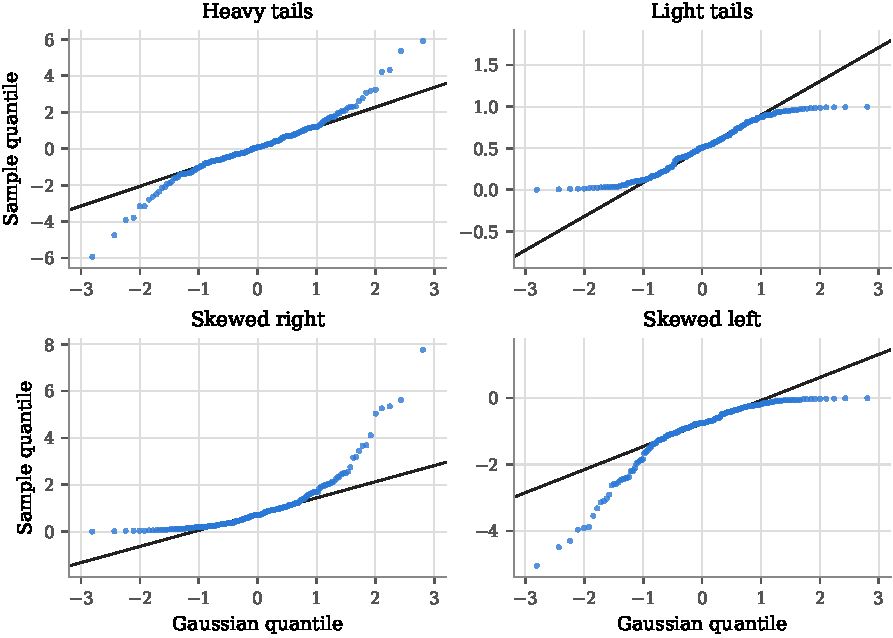
\includegraphics[width=\textwidth]{fig_qq_patterns}
\caption{Normal QQ plots of samples of $n = 200$ (blue), each with the line through its quartiles (black). Heavy tails: Student's $t$, $3$ degrees of freedom. Light tails: $\Unif(0, 1)$. Skewed right: $\Expo(1)$. Skewed left: minus an $\Expo(1)$.}
\label{fig:qqpatterns}
\end{figure}

\Cref{fig:qqreal} reads two real samples beside a simulated one.
On the left are $66$ standard Gaussians, for calibration: the points wander around the line, most at the ends, where order statistics are noisiest, and a pattern in a small sample should be judged against plots like this one.
In the middle, Newcomb's $64$ good measurements line up, and $-44$ and $-2$ sit far below the line; no test statistic points to the two culprits as directly.
On the right, Old Faithful's waits rise gently, then steeply, then gently again: two clumps, around $55$ and $80$ minutes, with few waits in between.

\begin{figure}[htbp]
\centering
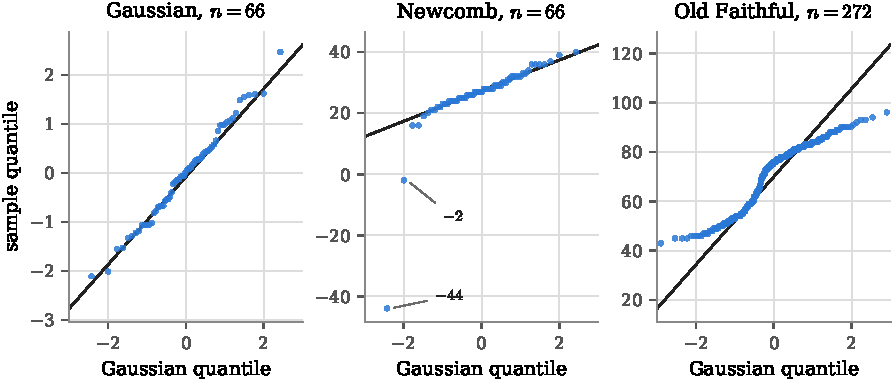
\includegraphics[width=\textwidth]{fig_qq_real}
\caption{Normal QQ plots (blue) with the line through the quartiles (black). Left: $66$ simulated standard Gaussians. Middle: Newcomb's $66$ measurements, nanoseconds above $24{,}800$. Right: Old Faithful's $272$ waits, in minutes.}
\label{fig:qqreal}
\end{figure}

The QQ plot and the Kolmogorov--Smirnov statistic compare the same two curves: the QQ plot measures the distance between them horizontally, at a fixed probability, and the statistic vertically, at a fixed $t$.
In the tails, where a CDF is nearly flat, two CDFs can be far apart horizontally and still close vertically: the extreme quantiles differ a lot while the probabilities differ little.
So the QQ plot magnifies the tails, which is where the Kolmogorov--Smirnov statistic hardly looks.

\section{What comes next}
\label{sec:ks-next}

Every method in the book so far has treated the parameter as a fixed unknown and the data as the only random thing.
\Cref{ch:bayes-intro} begins Part VII, where the parameter gets a distribution of its own: a prior, updated by the data into a posterior, with the kiss data's $p$ the first example.
The likelihood of \cref{ch:likelihood} is one of the two ingredients, and the answer is a distribution for $p$ rather than an interval or a test.

\section{Summary}
\label{sec:ks-summary}

\begin{itemize}[nosep]
\item The empirical CDF $F_n(t)$ is the proportion of the sample at or below $t$: at each $t$ a binomial proportion, with variance $F(t)(1 - F(t))/n$. Old Faithful: $F_{272}(60) = 0.305$.
\item Glivenko--Cantelli: $\sup_t\abs{F_n(t) - F(t)} \convp 0$ for every $F$, proved by cutting the line at finitely many quantiles and using monotonicity. The Kolmogorov distance can be estimated where total variation cannot.
\item Kolmogorov and Donsker: for continuous $F$, $\sqrt{n}\sup_t\abs{F_n(t) - F(t)} \convd K$, the largest absolute value of a Brownian bridge; $q_{0.05}(K) = 1.358$. The band $F_n \pm 1.358/\sqrt{n}$ covers $F$ with probability close to $95\%$ for large $n$ when $F$ is continuous, and with $1.3581$ in place of $1.358$ it covers $F$ with probability at least $95\%$ at every $n$, whatever $F$ is (Dvoretzky--Kiefer--Wolfowitz).
\item The Kolmogorov--Smirnov test of a stated continuous $F^0$ uses $D_n$, the largest of the $2n$ numbers $i/n - F^0(X_{(i)})$ and $F^0(X_{(i)}) - (i-1)/n$. By the probability integral transform its null distribution is the same for every continuous $F^0$; the test is consistent against every alternative.
\item Cram\'er--von Mises and Anderson--Darling add up squared gaps; Anderson--Darling divides each by its variance and so sees the tails. Binning for a chi-squared test loses power against shifts.
\item With parameters estimated, the Kolmogorov--Smirnov table gives a test that almost never rejects. For the Gaussian family the fitted statistic is pivotal, and the Lilliefors test simulates its null distribution: thresholds about $0.9/\sqrt{n}$ against $1.36/\sqrt{n}$. Newcomb: rejected with the two low values, not without them. Old Faithful: $0.155$ against $0.054$ ($0.063$ allowing for rounding).
\item A QQ plot pairs $X_{(i)}$ with $F^{-1}((i - \frac12)/n)$. A line means a good fit up to location and scale; heavy tails put the left end below the line and the right end above it, light tails bend both ends toward the horizontal, and skew bends the whole plot one way.
\end{itemize}

\section{Exercises}
\label{sec:ks-exercises}

\begin{exercise}
\label{ex:ks-pit}
Let $F$ be a continuous CDF, strictly increasing where $0 < F < 1$, and let $U \sim \Unif(0, 1)$. (a) Show that $F^{-1}(U)$ has CDF $F$. (b) For the exponential distribution with mean $5$, find $F^{-1}$, and turn the uniform values $0.08$ and $0.51$ into exponential waits. (c) Show that \cref{lem:pit} needs continuity: for $X \sim \Bern(\frac12)$, find the distribution of $F(X)$.
\end{exercise}
\begin{solution}
(a) For $x$ with $0 < F(x) < 1$, $F^{-1}(U) \leq x$ exactly when $U \leq F(x)$, since $F$ and $F^{-1}$ are increasing; so $\Pr(F^{-1}(U) \leq x) = \Pr(U \leq F(x)) = F(x)$. If $F(x) = 0$, then $F^{-1}(U)$, which lies where $0 < F < 1$, is above $x$, and both sides are $0$; if $F(x) = 1$, it is below $x$, and both sides are $1$. (b) $F(x) = 1 - e^{-x/5}$ for $x \geq 0$, so $F^{-1}(u) = -5\log(1 - u)$: $0.42$ and $3.57$ minutes, the first and fourth points of the right of \cref{fig:ksexample}. (c) $F(0) = \frac12$ and $F(1) = 1$, so $F(X)$ equals $\frac12$ or $1$, each with probability $\frac12$: not uniform.
\end{solution}

\begin{exercise}
\label{ex:ks-hand}
Five values are $0.8$, $0.7$, $0.4$, $0.7$ and $0.2$. Compute the Kolmogorov--Smirnov statistic for $H_0$: the data are $\Unif(0, 1)$, directly from the empirical CDF, and compare it with the exact $5\%$ threshold $d_{0.05}(5) = 0.563$ and with $1.358/\sqrt{5}$. What is odd about the data under a continuous null?
\end{exercise}
\begin{solution}
Sorted: $0.2, 0.4, 0.7, 0.7, 0.8$, so $F_5$ is $0.2$ from $0.2$, $0.4$ from $0.4$, $0.8$ from $0.7$ (two values) and $1$ from $0.8$. The gaps just below and at each step are $0.2$ and $0$ at $0.2$; $0.2$ and $0$ at $0.4$; $0.7 - 0.4 = 0.3$ and $0.8 - 0.7 = 0.1$ at $0.7$; $0$ and $0.2$ at $0.8$. So $D_5 = 0.3$, attained just below $0.7$. It is below the exact threshold $0.563$ and below $1.358/\sqrt{5} = 0.607$ (equivalently, $\sqrt{5}D_5 = 0.67 < 1.358$): do not reject. The value $0.7$ appears twice, which has probability $0$ under a continuous distribution; the data were rounded or made up. (The formula of \cref{prop:ks-compute}, applied to the five sorted values, gives the same $0.3$.)
\end{solution}

\begin{exercise}
\label{ex:ks-cov}
Let $G_n$ be the empirical CDF of $n$ i.i.d.\ $\Unif(0, 1)$ variables and $0 < u < v < 1$. (a) Show that $\sqrt{n}(G_n(u) - u)$ and $\sqrt{n}(G_n(v) - v)$ have covariance $u(1 - v)$. (b) Show that the pair converges in distribution to a Gaussian vector with this covariance, checking that the covariance matrix is positive definite. (c) Where is the limiting variance largest, and what is the correlation of the limit at $u = \frac14$ and $v = \frac34$?
\end{exercise}
\begin{solution}
(a) \Cref{prop:ecdf-pointwise} with $F(u) = u$ gives $\cov(G_n(u), G_n(v)) = u(1 - v)/n$; multiply by $n$. (b) The pair is $\sqrt{n}(\bar{Y}_n - m)$ with $Y_i = (\ind(U_i \leq u), \ind(U_i \leq v))$, $m = (u, v)$ and covariance matrix with diagonal $u(1 - u)$, $v(1 - v)$ and off-diagonal $u(1 - v)$. The diagonal is positive and the determinant is $u(1 - u)v(1 - v) - u^2(1 - v)^2 = u(1 - v)(v - u) > 0$, so the matrix is positive definite, and the CLT for vectors gives the Gaussian limit. (c) The variance $u(1 - u)$ is largest at $u = \frac12$, where it is $\frac14$. At $\frac14$ and $\frac34$ the covariance is $\frac14 \times \frac14 = \frac1{16}$ and each variance is $\frac3{16}$, so the correlation is $\frac13$.
\end{solution}

\begin{exercise}
\label{ex:ks-discrete}
For the kiss data and $F^0$ the CDF of $\Bern(\frac12)$: (a) show that $D_n = \abs{\hat{p} - \frac12}$ and that $\sqrt{n}D_n = \abs{T_n}/2$, where $T_n = \sqrt{n}(\hat{p} - \frac12)/\frac12$ is the statistic of \cref{ch:tests-foundations}; (b) under $H_0$, find the limit of $\sqrt{n}D_n$ and the limit of the probability that it exceeds $1.358$; (c) say which step of the proof of \cref{thm:ks} fails.
\end{exercise}
\begin{solution}
(a) $F_n - F^0$ is $0$ for $t < 0$ and for $t \geq 1$, and $(1 - \hat{p}) - \frac12 = \frac12 - \hat{p}$ for $0 \leq t < 1$, so $D_n = \abs{\hat{p} - \frac12}$, and $\sqrt{n}D_n = \sqrt{n}\abs{\hat{p} - \frac12} = \abs{T_n}/2$. (b) $T_n \convd \Gauss(0, 1)$ by the CLT (\cref{thm:clt}), so by the continuous mapping theorem (\cref{thm:cmt}: if $T_n \convd T$ and $g$ is continuous, $g(T_n) \convd g(T)$; here $g(t) = \abs{t}/2$), $\sqrt{n}D_n \convd \abs{Z}/2$ with $Z \sim \Gauss(0, 1)$, and $\Pr(\abs{Z}/2 > 1.358) = \Pr(\abs{Z} > 2.716) = 0.0066$. (At $n = 124$ the threshold rejects for $46$ or fewer or $78$ or more right turns, probability $0.0052$.) (c) \Cref{lem:pit}: $F^0(X)$ takes only the values $\frac12$ and $1$, so the transformed data are not uniform.
\end{solution}

\begin{exercise}
\label{ex:ks-band}
Of the $272$ Old Faithful waits, $83$ are at most $60$ minutes. (a) Compute the plug-in $95\%$ interval for $F(60)$ and the $95\%$ band of \cref{sec:ks-donsker} at $60$. (b) Why is the band wider? (c) The Gaussian CDF closest to the empirical CDF in Kolmogorov distance is $0.102$ away. What does the band say about the Gaussian family, and at what level?
\end{exercise}
\begin{solution}
(a) $0.305 \pm 1.96\sqrt{0.305 \times 0.695/272} = 0.305 \pm 0.055 = [0.250, 0.360]$, and $0.305 \pm 1.358/\sqrt{272} = 0.305 \pm 0.082 = [0.223, 0.387]$. (b) The interval covers $F(60)$ alone with probability about $95\%$; the band must cover $F(t)$ at every $t$ at once, and the largest of $\sqrt{n}\abs{F_n(t) - F(t)}$ over all $t$ is larger than its value at one point: $1.358$ against $1.96\sqrt{0.305 \times 0.695} = 0.90$ at $t = 60$. (c) Every Gaussian CDF is somewhere at least $0.102 > 0.082$ from the staircase, so every Gaussian leaves the band. If the waits were Gaussian, the band with half-width $1.3581/\sqrt{272}$, also $0.082$, would contain their CDF with probability at least $95\%$, so this rejects the whole Gaussian family at level $5\%$. (Rounding the Gaussian to the minute, as the waits are, still leaves it $0.092$ away.)
\end{solution}

\begin{exercise}
\label{ex:ks-tv}
(a) Show that the Kolmogorov distance between two distributions is at most their total variation distance. (b) For $\Expo(1)$ and $\Gauss(1, 1)$ the Kolmogorov distance is $0.159$ and the total variation distance is $0.319$; explain the value $0.159$. (c) For a sample from a continuous $F$, the empirical distribution is at total variation distance $1$ from $F$ at every $n$ (\cref{sec:dist-tv-estimate}). Why does its Kolmogorov distance from $F$ tend to $0$ all the same?
\end{exercise}
\begin{solution}
(a) Let $\Pr$ and $\Qr$ have CDFs $F$ and $G$. For each $t$, $\abs{F(t) - G(t)} = \abs{\Pr(A) - \Qr(A)}$ with $A = (-\infty, t]$, which is at most the supremum over all events, the total variation distance. (b) At $t = 0$ the Gaussian puts $\Phi(-1) = 0.159$ below $0$ and the exponential puts nothing there. For $t < 0$ the gap is $\Phi(t - 1)$, smaller still. For $t > 0$ the gap first shrinks; the exponential CDF then runs above the Gaussian one between $t = 0.26$ and $t = 2.25$, by at most $0.133$ (at $t = 0.92$, where the densities cross), and beyond $t = 2.25$ below it, by at most $0.027$ (at $t = 3.08$, where they cross again). So $0.159$ is the largest gap. (c) Total variation compares all events, including the finite set of observed values, which has empirical probability $1$ and probability $0$ under $F$. The Kolmogorov distance compares only half-lines, and \cref{thm:glivenko-cantelli} controls all of them at once.
\end{solution}

\begin{exercise}
\label{ex:ks-cvm}
Let $U_{(1)} < \cdots < U_{(n)}$ be the order statistics of $U_i = F^0(X_i)$, with $U_{(0)} = 0$ and $U_{(n+1)} = 1$. (a) Show that $W^2_n = n\int_0^1(G_n(u) - u)^2\,\mathrm{d}u$, with $G_n$ the empirical CDF of the $U_i$. (b) Using that $G_n = i/n$ on $[U_{(i)}, U_{(i+1)})$, show that $W^2_n = \frac1{12n} + \sum_i\big(U_{(i)} - \frac{2i-1}{2n}\big)^2$. (c) Compute $W^2_{10}$ for the ten generator outputs of the worked example in \cref{sec:ks-test}, and compare it with the $5\%$ threshold $0.46$.
\end{exercise}
\begin{solution}
(a) Substitute $u = F^0(t)$, $\mathrm{d}u = f^0(t)\,\mathrm{d}t$, and use $F_n(t) = G_n(F^0(t))$ from the proof of \cref{thm:ks}. (b) $\int_{U_{(i)}}^{U_{(i+1)}}(i/n - u)^2\,\mathrm{d}u = \frac13\big[(U_{(i+1)} - \frac{i}{n})^3 - (U_{(i)} - \frac{i}{n})^3\big]$. Summing over $i = 0, \ldots, n$, the terms at $U_{(0)} = 0$ and $U_{(n+1)} = 1$ vanish, and each $U_{(i)}$ with $1 \leq i \leq n$ contributes $\frac13\big[(U_{(i)} - \frac{i-1}{n})^3 - (U_{(i)} - \frac{i}{n})^3\big]$. With $a_i = U_{(i)} - \frac{2i-1}{2n}$ this is $\frac13\big[(a_i + \frac1{2n})^3 - (a_i - \frac1{2n})^3\big] = \frac{a_i^2}{n} + \frac1{12n^3}$. Multiplying the sum by $n$ gives $\sum_ia_i^2 + \frac1{12n}$. (c) The differences $a_i$ are $0.03, 0.02, 0.13, 0.16, 0.09, 0.06, 0.15, 0.12, 0.09, 0.03$, whose squares add up to $0.1014$; with $\frac1{120} = 0.0083$, $W^2_{10} = 0.110$, far below $0.46$.
\end{solution}

\begin{exercise}
\label{ex:ks-expo}
For the exponential family, let $\hat{D}_n = \sup_{t \geq 0}\abs{F_n(t) - (1 - e^{-t/\bar{X}_n})}$, the largest gap to the exponential distribution with the sample mean as its mean. Show that if the $X_i$ are i.i.d.\ $\Expo(\lambda)$, the distribution of $\hat{D}_n$ does not depend on $\lambda$, so that its thresholds can be found by simulating $\Expo(1)$ samples.
\end{exercise}
\begin{solution}
Write $X_i = Y_i/\lambda$ with $Y_1, \ldots, Y_n \iid \Expo(1)$, so $\bar{X}_n = \bar{Y}_n/\lambda$. For $t \geq 0$ put $s = \lambda t$: $X_i \leq t$ exactly when $Y_i \leq s$, so $F_n(t) = F^Y_n(s)$, and $t/\bar{X}_n = s/\bar{Y}_n$. As $t$ runs over $[0, \infty)$ so does $s$, so $\hat{D}_n = \sup_{s \geq 0}\abs{F^Y_n(s) - (1 - e^{-s/\bar{Y}_n})}$, a function of the $Y_i$ alone.
\end{solution}

\begin{exercise}
\label{ex:ks-qq-skew}
For $X \sim \Expo(1)$, the normal QQ plot of a large sample lies near the curve $h(x) = F^{-1}(\Phi(x)) = -\log(1 - \Phi(x))$. (a) Compute $h(-2)$, $h(0)$ and $h(2)$, using $\Phi(-2) = 0.023$. (b) Compare the slopes of the chords from $-2$ to $0$ and from $0$ to $2$, and explain the upward bend of the skewed-right plot in \cref{fig:qqpatterns}. (c) What is the curve for $\Unif(0, 1)$ data, and how does it explain the light-tailed plot?
\end{exercise}
\begin{solution}
(a) $h(-2) = -\log(0.977) = 0.023$, $h(0) = \log 2 = 0.693$ and $h(2) = -\log(0.023) = 3.77$. (b) The slopes are $(0.693 - 0.023)/2 = 0.335$ and $(3.77 - 0.693)/2 = 1.54$, more than four times larger on the right: the long right tail stretches the upper quantiles and the short left tail squeezes the lower ones, so the points bend upward. (c) $h(x) = \Phi(x)$, which flattens toward $0$ on the left and toward $1$ on the right: the ends of a uniform sample are closer to the middle than Gaussian ends would be, the light-tailed pattern.
\end{solution}


\partintro{The one part of the book where the parameter gets a distribution. Priors, posteriors and conjugacy (\cref{ch:bayes-intro}) set up the machinery; Jeffreys priors and Bayesian confidence regions (\cref{ch:jeffreys}) finish it, and say how the result relates to the frequentist intervals of \cref{ch:confidence-intervals}.}
\part{Bayesian Statistics}
\chapter{Priors, Posteriors and Conjugacy}
\label{ch:bayes-intro}

\begin{chaptergoals}
\begin{itemize}[nosep]
\item The Bayesian model: a prior distribution for the parameter, the statistical model read as the distribution of the data given the parameter, and the posterior that Bayes' formula makes from the two. Computed first on a grid of nine values of the kiss proportion.
\item Conjugate priors, which keep the posterior in the prior's family: Beta for a proportion, Gamma for a rate, Gaussian for a mean. The kiss data, the subway waits and the wind turbine, and the prior read as extra observations.
\item Updating one observation at a time, and why it gives the same posterior as all the data at once.
\item Summaries of the posterior: the posterior mean, which is best under squared error, the median, the mode, and the probability that the next couple turns right.
\item Probabilities of intervals and of hypotheses: with a flat prior they come close to confidence levels and one-sided $p$-values while answering a different question, and a point null gets a very different number. The Bernstein--von Mises theorem: with enough data the prior stops mattering, and the posterior is the Gaussian of \cref{ch:mle-properties}.
\end{itemize}
\Cref{ch:ks} ended the book's tests, all of which treated the parameter as a fixed unknown number. This chapter gives it a distribution.
\end{chaptergoals}

\section{A distribution for the parameter}
\label{sec:bayes-why}

Every chapter so far has treated $p$, the proportion of couples who turn their heads to the right, as a fixed unknown number.
The data are random and $p$ is not, so every conclusion has been a statement about a procedure: an interval that covers $p$ in $95\%$ of repetitions, a test that rejects a true null $5\%$ of the time.
\Cref{ch:confidence-intervals} named the statement most people want instead, `the probability that $p$ is between $0.56$ and $0.73$ is $0.95$', and noted that it needs $p$ to have a distribution.

The Bayesian approach gives it one.
Before the data, what is known about $p$ is described by a probability distribution, the \textbf{prior}; after the data, by the conditional distribution of $p$ given the data, the \textbf{posterior}.
The model for the data is the one used all along, now read as the distribution of the data given $p$.
Nothing here claims that $p$ is random in the world: the couples have whatever preference they have.
The distribution describes knowledge about $p$, and the data change the knowledge.
That is the difference \cref{ch:kiss} promised, and the rest of the chapter computes with it.

A prior can be read in three ways, and the mathematics is the same for all of them.
As a degree of belief: someone who is $90\%$ sure that $p$ lies between $0.4$ and $0.6$ can write that down as a distribution, and the rules of probability are what keep such beliefs consistent (if someone's betting odds break those rules, a bookmaker can choose bets against them that win whatever happens: the Dutch book argument).
As a state of information: what was known before the study, from earlier studies or from constraints such as $0 \leq p \leq 1$.
As a device: a way to build estimators, which are then judged by the criteria of \cref{ch:estimators} like any others.

\begin{bridge}[Bayes' rule]
An introductory course states Bayes' rule for two events, often with a medical test: the probability of the disease given a positive test is the probability of a positive test given the disease, times the prevalence, divided by the overall probability of a positive test.
The formula of this chapter is the same rule with `the parameter equals $\theta$' in place of the disease and the observed data in place of the positive test.
The prevalence becomes the prior, the test's accuracy becomes the likelihood, and the answer is the posterior.
The denominator, the overall chance of what was observed, adds the numerator up over every value the parameter could take.
\end{bridge}

\section{Bayes' formula for a parameter}
\label{sec:bayes-formula}

Start with a parameter that can take only finitely many values, where the rule is the one for events.
Suppose that before the kiss study $p$ was thought equally likely to be any of $0.1, 0.2, \ldots, 0.9$: prior probability $\frac19$ each.
A sequence of $124$ outcomes with $80$ right turns has probability $p^{80}(1 - p)^{44}$ under each candidate (the probability of exactly $80$ right turns in any order adds a binomial coefficient, the same for every candidate, which cancels).
Bayes' rule multiplies each prior probability by this likelihood and divides by the sum over the nine candidates:
\[
\Pr(p = 0.6 \mid \text{data}) = \frac{\frac19 \cdot 0.6^{80}\,0.4^{44}}{\sum_{j=1}^9 \frac19 (j/10)^{80}(1 - j/10)^{44}} = 0.58.
\]
The prior probabilities cancel, since they are equal, and what remains is the likelihood at $0.6$ as a share of its sum over the grid.
In natural frequencies: picture $900{,}000$ repetitions of the study, $100{,}000$ for each candidate.
Of the $100{,}000$ with $p = 0.6$, about $4{,}378$ see exactly $80$ right turns; of those with $p = 0.7$, about $3{,}160$; with $p = 0.5$, about $37$; with $p = 0.8$, about $2$; with the other five values, essentially none.
Among the roughly $7{,}580$ repetitions that saw what was seen, $58\%$ had $p = 0.6$, $42\%$ had $p = 0.7$, and half a percent had $p = \frac12$.
That is the posterior, drawn in \cref{fig:bayesgrid}: the likelihood decides which candidates survive, and the prior, flat here, decides nothing.

\begin{figure}[htbp]
\centering
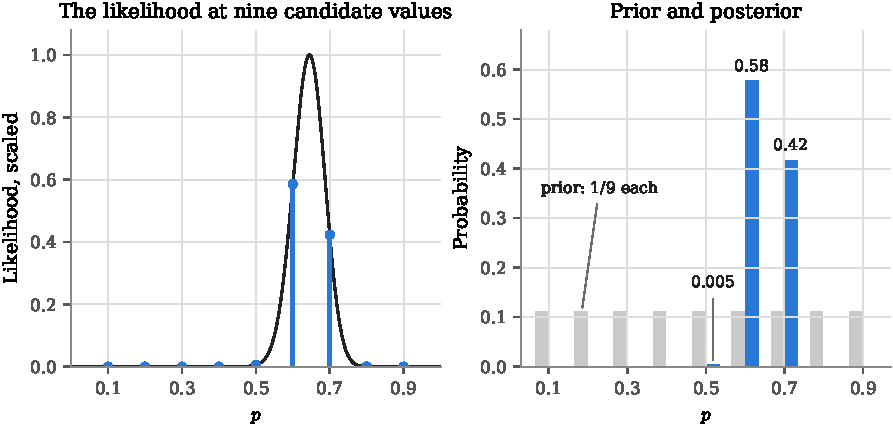
\includegraphics[width=\textwidth]{fig_bayes_grid}
\caption{The kiss data and a prior of $\frac19$ on each of $p = 0.1, 0.2, \ldots, 0.9$. Left: the likelihood $p^{80}(1 - p)^{44}$ scaled to maximum $1$ (black) and its values at the nine candidates (blue). Right: prior (gray) and posterior (blue).}
\label{fig:bayesgrid}
\end{figure}

For a parameter that varies continuously, sums become integrals.

\begin{definition}[Prior and posterior]
\label{def:posterior}
Let $(E, (\Pr_\theta)_{\theta \in \Theta})$ be a statistical model for $\Xton$ with likelihood $L_n(x_1, \ldots, x_n; \theta)$ (\cref{def:likelihood-discrete,def:likelihood-continuous}), and write $\mathbf{x} = (x_1, \ldots, x_n)$. A \textbf{prior} is a probability distribution on $\Theta$ with density $\pi$, or with PMF $\pi$ when $\Theta$ is finite or countable (this $\pi$ is unrelated to the mixture weight of \cref{ch:models,ch:likelihood}). The \textbf{Bayesian model} takes $\theta$ random with distribution $\pi$ and, given $\theta$, the observations i.i.d.\ $\Pr_\theta$. The \textbf{posterior} is the conditional distribution of $\theta$ given $X_1 = x_1, \ldots, X_n = x_n$, with density (or PMF)
\[
\pi(\theta \mid \mathbf{x}) = \frac{L_n(\mathbf{x}; \theta)\,\pi(\theta)}{m(\mathbf{x})}, \qquad m(\mathbf{x}) = \int_\Theta L_n(\mathbf{x}; t)\,\pi(t)\,\mathrm{d}t,
\]
defined whenever $0 < m(\mathbf{x}) < \infty$, with a sum in place of the integral when $\Theta$ is finite or countable. The denominator $m(\mathbf{x})$ is the \textbf{marginal likelihood} of the data.
\end{definition}

\begin{inwords}
\textbf{In words.} Posterior is likelihood times prior, rescaled to total probability $1$. Both are read as functions of $\theta$ with the data held fixed, and the marginal likelihood is the rescaling constant: the probability, or density, that the model and the prior together gave the data before they were seen.
\par\smallskip
\textbf{For the kiss data.} The likelihood is $L_n = p^{80}(1 - p)^{44}$, and with the flat prior $\pi(p) = 1$ on $(0, 1)$ the posterior density is $p^{80}(1 - p)^{44}/m$, where $m = \int_0^1 t^{80}(1 - t)^{44}\,\mathrm{d}t$. It is the black curve on the left of \cref{fig:bayesgrid}, rescaled to be a density.
\end{inwords}

The condition $0 < m(\mathbf{x}) < \infty$ rules out two things: data that every allowed $\theta$ calls impossible, where $m(\mathbf{x}) = 0$, and a likelihood so large over some values of $\theta$ that the integral diverges, which cannot happen for discrete data, since then $L_n \leq 1$ and so $m(\mathbf{x}) \leq 1$.
The condition holds in every example of this chapter.
The formula is the definition of a conditional density.
The joint density of the parameter and the data is $\pi(\theta)L_n(\mathbf{x}; \theta)$, the density of $\theta$ times the density of the data given $\theta$; the density of the data alone is this joint density integrated over $\theta$, which is $m(\mathbf{x})$; and a conditional density is a joint density divided by the density of what is conditioned on, the continuous version of $\Pr(A \mid B) = \Pr(A \cap B)/\Pr(B)$.
The same formula covers four cases: a parameter that is discrete or continuous, and data that are discrete or continuous.
For discrete data $L_n$ is a product of PMFs and for continuous data a product of densities; for a discrete parameter $m$ is a sum over $\Theta$ and for a continuous one an integral. (With discrete data and a continuous parameter the joint distribution is a PMF in the data and a density in $\theta$.)

Since $m(\mathbf{x})$ does not depend on $\theta$, it never needs computing to find the shape of the posterior.
A nonnegative function with a finite, nonzero integral is proportional to exactly one density, so it is enough to compute $L_n(\mathbf{x}; \theta)\pi(\theta)$, drop every factor that does not involve $\theta$, and recognize what is left.
The symbol $\propto$, `is proportional to as a function of $\theta$', records this:
\[
\pi(\theta \mid \mathbf{x}) \propto L_n(\mathbf{x}; \theta)\,\pi(\theta).
\]

\begin{pitfall}[a prior of zero cannot be undone]
Where $\pi(\theta) = 0$, the product $L_n\pi$ is $0$, so the posterior is $0$ there whatever the data say.
In the grid of \cref{fig:bayesgrid}, the value $0.645$ had prior probability $0$, and the posterior puts nearly all its weight on its two neighbors, $0.6$ and $0.7$.
A prior uniform on $[0.3, 0.8]$ would rule out every $p$ above $0.8$ for good, even if every couple turned right.
A prior should give some probability to every value that is not impossible.
\end{pitfall}

\section{The Beta prior for a proportion}
\label{sec:bayes-beta}

A grid works, but a family of densities on $(0, 1)$ that matches the shape of the likelihood does better.

\begin{definition}[The Beta distribution]
\label{def:beta}
For $a, b > 0$, the \textbf{Beta distribution} $\Betad(a, b)$ has density
\[
f(p) = \frac{p^{a-1}(1 - p)^{b-1}}{B(a, b)}, \qquad 0 < p < 1, \qquad B(a, b) = \int_0^1 t^{a-1}(1 - t)^{b-1}\,\mathrm{d}t = \frac{\Gamma(a)\Gamma(b)}{\Gamma(a + b)},
\]
where $\Gamma(a) = \int_0^\infty t^{a-1}e^{-t}\,\mathrm{d}t$, so that $\Gamma(k) = (k - 1)!$ for $k = 1, 2, 3, \ldots$. Its mean is $a/(a + b)$, its variance $ab/\big((a + b)^2(a + b + 1)\big)$, and, when $a, b > 1$, its mode is $(a - 1)/(a + b - 2)$ (\cref{ex:bayes-beta-moments}). $\Betad(1, 1)$ is $\Unif(0, 1)$.
\end{definition}

\begin{inwords}
\textbf{In words.} A flexible family on $(0, 1)$: a larger $a$ pulls the mass toward $1$, a larger $b$ toward $0$, and $a + b$ sets how concentrated it is.
\par\smallskip
\textbf{For the kiss data.} $\Betad(1, 1)$ is the flat prior. $\Betad(33, 33)$ has mean $\frac12$ and puts $90\%$ of its probability between $0.4$ and $0.6$: the prior of a skeptic who doubts a strong preference either way.
\end{inwords}

\begin{theorem}[Beta prior, Bernoulli data]
\label{thm:beta-bernoulli}
Let $p \sim \Betad(a, b)$ and, given $p$, let $\Xton$ be i.i.d.\ $\Bern(p)$, with $S = \sum_i X_i$. The posterior is $\Betad(a + S, b + n - S)$.
\end{theorem}

\coreproof{Multiply the prior by the likelihood and keep only what depends on $p$: what is left has the shape of a Beta density, with each exponent raised by a count.}
\begin{proof}
By \cref{def:posterior},
\[
\pi(p \mid \mathbf{x}) \propto p^S(1 - p)^{n - S} \cdot \frac{p^{a-1}(1 - p)^{b-1}}{B(a, b)} \propto p^{a + S - 1}(1 - p)^{b + n - S - 1}, \qquad 0 < p < 1.
\]
Up to a constant this is the $\Betad(a + S, b + n - S)$ density, and since both integrate to $1$ the constant is $1$.
\end{proof}

\begin{intuition}[the prior as imaginary couples]
The parameters tell the story: updating adds the $S$ right turns to $a$ and the $n - S$ left turns to $b$, so in the posterior $a$ and $b$ play the part of right and left turns seen before the study.
The posterior mean is
\[
\frac{a + S}{a + b + n} = w\,\frac{a}{a + b} + (1 - w)\,\frac{S}{n}, \qquad w = \frac{a + b}{a + b + n},
\]
a weighted average of the prior mean and the sample proportion, with the prior weighted by its $a + b$ imaginary couples against the $n$ real ones.
For the kiss data the flat prior counts as $2$ imaginary couples in the posterior mean (its density, $p^0(1 - p)^0$, adds nothing to the likelihood), weight $w = 2/126 = 0.016$, and the posterior mean is $81/126 = 0.643$; $\Betad(10, 10)$ is $20$ couples, $w = 0.139$, mean $90/144 = 0.625$; the skeptic's $\Betad(33, 33)$ is $66$ couples, $w = 0.347$, mean $113/190 = 0.595$.
As $n$ grows with the prior fixed, $w$ falls like $1/n$.
\end{intuition}

\Cref{fig:bayesbeta} draws the three priors and their posteriors.
The flat prior's posterior, $\Betad(81, 45)$, is the likelihood made into a density, with standard deviation $0.043$.
The skeptic's posterior, $\Betad(113, 77)$, is pulled a third of the way back toward $\frac12$, yet even the skeptic now puts probability $0.996$ on $p > \frac12$. The $124$ couples persuade someone who started $90\%$ sure that any preference was weak that couples do prefer the right, though not that the preference is strong: the skeptic still puts $0.56$ on $p < 0.6$.

\begin{figure}[htbp]
\centering
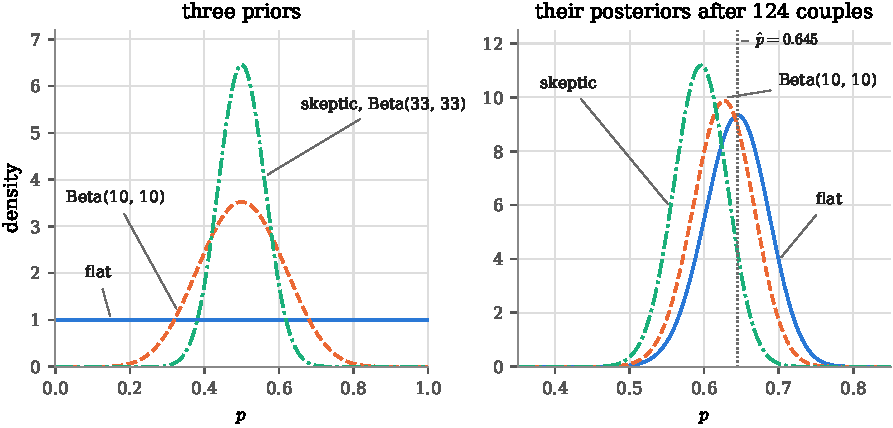
\includegraphics[width=\textwidth]{fig_bayes_beta}
\caption{Left: the priors $\Betad(1, 1)$ (blue), $\Betad(10, 10)$ (orange, dashed) and the skeptic's $\Betad(33, 33)$ (aqua, dash-dot). Right: their posteriors after $80$ right turns among $124$ couples, and $\hat{p} = 0.645$ (dotted).}
\label{fig:bayesbeta}
\end{figure}

The shrinkage estimator $(n\bar{R}_n + 10)/(n + 20)$ of \cref{sec:est-risk}, which pulled the estimate toward $\frac12$ `as if $20$ extra coin flips had come up half heads', is the posterior mean under the $\Betad(10, 10)$ prior: $90/144 = 0.625$ for the kiss data.
The imaginary flips are the prior's $a + b = 20$ couples.
\Cref{ch:estimators} found that it has lower risk than $\bar{R}_n$ when $p$ is near $\frac12$ and higher risk far from it, which in Bayesian terms says that it does best where its prior puts the weight.

\begin{bridge}[the plus-four estimate]
The plus-four interval of \cref{sec:ci-coverage}, taught in some introductory courses, adds two successes and two failures and is centered at $\tilde{p} = (S + 2)/(n + 4)$ in place of $\hat{p}$.
The estimate $\tilde{p}$ is the posterior mean under the $\Betad(2, 2)$ prior. For the kiss data it is $82/128 = 0.641$.
\end{bridge}

\begin{definition}[Conjugate prior]
\label{def:conjugate}
A family of priors is \textbf{conjugate} for a statistical model if, for every prior in the family and every sample, the posterior is again in the family.
\end{definition}

\begin{inwords}
\textbf{In words.} With a conjugate prior, updating changes the parameters of the prior and nothing else, so the posterior is a formula instead of an integral to compute.
\par\smallskip
\textbf{For the kiss data.} The Beta family is conjugate for Bernoulli data (\cref{thm:beta-bernoulli}): updating adds the number of right turns to $a$ and the number of left turns to $b$.
\end{inwords}

\begin{sanitycheck}[Where must the posterior mean land?]
Between the prior mean and the sample proportion, by the weighted average above, and closer to whichever stands for more couples.
A posterior mean outside $[0.5, 0.645]$ for a prior with mean $\frac12$ and the kiss data signals an arithmetic error.
The skeptic's $0.595$ passes: $0.347 \times 0.5 + 0.653 \times 0.645 = 0.595$.
\end{sanitycheck}

\section{Rates and means: two more conjugate pairs}
\label{sec:bayes-conjugate}

A rate can be any positive number and a mean any real number, so neither fits a prior on $(0, 1)$.
For a rate the conjugate family is the Gamma.

\begin{definition}[The Gamma distribution]
\label{def:gamma}
For $\alpha, \beta > 0$, the \textbf{Gamma distribution} $\Gammad(\alpha, \beta)$, with shape $\alpha$ and rate $\beta$, has density
\[
f(\lambda) = \frac{\beta^\alpha\lambda^{\alpha - 1}e^{-\beta\lambda}}{\Gamma(\alpha)}, \qquad \lambda > 0,
\]
with mean $\alpha/\beta$ and variance $\alpha/\beta^2$. $\Gammad(1, \beta)$ is $\Expo(\beta)$.
\end{definition}

\begin{inwords}
\textbf{In words.} A flexible family on $(0, \infty)$, the natural home for a rate. Its mean $\alpha/\beta$ reads as $\alpha$ events in a time $\beta$.
\par\smallskip
\textbf{For the kiss data.} The kiss proportion lives in $(0, 1)$, so its prior is a Beta, not a Gamma; the Gamma is for the subway rate $\lambda$, trains per minute, which can be any positive number.
\end{inwords}

\begin{proposition}[Gamma prior, exponential data]
\label{prop:gamma-expo}
Let $\lambda \sim \Gammad(\alpha, \beta)$ and, given $\lambda$, let $T_1, \ldots, T_n$ be i.i.d.\ $\Expo(\lambda)$. The posterior is $\Gammad\big(\alpha + n, \beta + \sum_i T_i\big)$.
\end{proposition}

\optionalproof{The same recognition as for the Beta: the likelihood $\lambda^n e^{-\lambda\sum T_i}$ has the shape of a Gamma density in $\lambda$.}
\begin{proof}
$\pi(\lambda \mid \mathbf{t}) \propto \lambda^n e^{-\lambda\sum_i t_i} \cdot \lambda^{\alpha - 1}e^{-\beta\lambda} = \lambda^{\alpha + n - 1}e^{-(\beta + \sum_i t_i)\lambda}$ for $\lambda > 0$, the shape of the $\Gammad(\alpha + n, \beta + \sum_i t_i)$ density.
\end{proof}

In the posterior's parameters the prior again acts as imaginary data, here $\alpha$ waits lasting $\beta$ minutes in total.
For the subway, suppose the timetable promises a train every $5$ minutes, and take a prior with mean $0.2$ trains per minute that counts as $30$ waits: $\Gammad(30, 150)$.
The $64$ observed waits total $64 \times 6.23 = 398.7$ minutes, so the posterior is $\Gammad(94, 548.7)$, with mean $94/548.7 = 0.171$ and standard deviation $\sqrt{94}/548.7 = 0.018$.
The maximum likelihood estimate is $1/6.23 = 0.161$. The reciprocal of the posterior mean, $548.7/94 = 5.84$ minutes per train, is the average of the timetable's $5$ and the observed $6.23$, weighted by $30$ imaginary waits and $64$ real ones.

\begin{proposition}[Gaussian prior, Gaussian data with known variance]
\label{prop:normal-normal}
Let $\mu \sim \Gauss(\mu_0, \sigma_0^2)$ and, given $\mu$, let $\Xton$ be i.i.d.\ $\Gauss(\mu, \sigma^2)$ with $\sigma^2$ known. The posterior is $\Gauss(\mu_n, \sigma_n^2)$ with
\[
\frac{1}{\sigma_n^2} = \frac{1}{\sigma_0^2} + \frac{n}{\sigma^2}, \qquad \mu_n = \sigma_n^2\Big(\frac{\mu_0}{\sigma_0^2} + \frac{n\bar{x}_n}{\sigma^2}\Big).
\]
\end{proposition}

\optionalproof{Multiply the two Gaussian shapes; the exponent is a quadratic in $\mu$, and completing the square names its center and spread.}
\begin{proof}
Using $\sum_i(x_i - \mu)^2 = \sum_i(x_i - \bar{x}_n)^2 + n(\bar{x}_n - \mu)^2$ and dropping factors free of $\mu$,
\[
\pi(\mu \mid \mathbf{x}) \propto \exp\Big(-\frac{n(\mu - \bar{x}_n)^2}{2\sigma^2} - \frac{(\mu - \mu_0)^2}{2\sigma_0^2}\Big) \propto \exp\Big(-\frac{\mu^2}{2}\Big(\frac{n}{\sigma^2} + \frac{1}{\sigma_0^2}\Big) + \mu\Big(\frac{n\bar{x}_n}{\sigma^2} + \frac{\mu_0}{\sigma_0^2}\Big)\Big).
\]
Since $-\frac{\mu^2}{2\sigma_n^2} + \frac{\mu\mu_n}{\sigma_n^2} = -\frac{(\mu - \mu_n)^2}{2\sigma_n^2} + \frac{\mu_n^2}{2\sigma_n^2}$, the last expression is proportional to $\exp\big(-(\mu - \mu_n)^2/(2\sigma_n^2)\big)$, the shape of the $\Gauss(\mu_n, \sigma_n^2)$ density.
\end{proof}

The reciprocal of a variance is a \textbf{precision}, and the proposition says that precisions add: the prior contributes $1/\sigma_0^2$, each observation $1/\sigma^2$, and the posterior mean is the average of $\mu_0$ and $\bar{x}_n$ weighted by their precisions.
The prior counts as $\sigma^2/\sigma_0^2$ observations.
The same calculation works when the observations have different known variances $\sigma_i^2$: each $x_i$ is weighted by $1/\sigma_i^2$, and the prior mean enters as one more observation with variance $\sigma_0^2$.

\Cref{ch:t-test} asked whether the mean wind speed $\mu$ at a home is above $10$ miles per hour, from $12$ monthly measurements with mean $14.3$ and standard deviation $4.7$.
Take $\sigma = 4.7$ as known, and a prior centered at $11$, a regional average, with standard deviation $2$.
The prior counts as $4.7^2/2^2 = 5.5$ months of data, so the posterior mean is $(5.5 \times 11 + 12 \times 14.3)/17.5 = 13.26$ and the posterior standard deviation is $4.7/\sqrt{17.5} = 1.12$.
Where the $t$-test of \cref{ch:t-test} rejected $\mu \leq 10$, the posterior gives a probability: $\Pr(\mu > 10 \mid \text{data}) = 1 - \Phi\big((10 - 13.26)/1.12\big) = 0.998$.
(Treating $\sigma$ as unknown needs a prior for $\sigma$ too. With $\sigma$ independent of $\mu$ and a prior density proportional to $1/\sigma$, a common choice that \cref{ch:jeffreys} explains, the probability is $0.991$. That density has an infinite integral, so it is not a probability distribution and \cref{def:posterior} does not cover it; \cref{ch:jeffreys} says why the posterior is still a proper distribution.)
\Cref{fig:bayesconj} draws both examples, and in both the posterior lies between the prior and the likelihood and is narrower than either; on the right, the area under the posterior to the right of the gray line at $10$ is the $0.998$ above.

\begin{figure}[htbp]
\centering
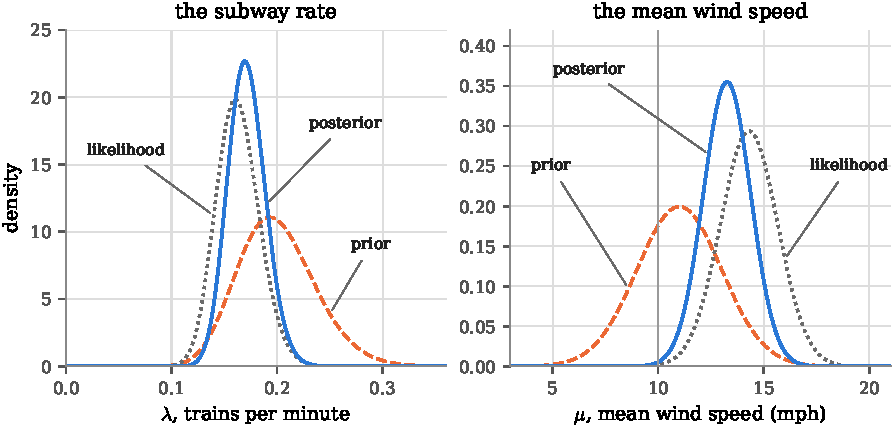
\includegraphics[width=\textwidth]{fig_bayes_conjugate}
\caption{Prior (orange, dashed), likelihood scaled to a density (gray, dotted) and posterior (blue). Left: the subway rate, prior $\Gammad(30, 150)$, posterior $\Gammad(94, 548.7)$. Right: the mean wind speed, prior $\Gauss(11, 2^2)$, posterior $\Gauss(13.26, 1.12^2)$; gray line at $10$.}
\label{fig:bayesconj}
\end{figure}

\begin{center}
\small
\begin{tabular}{@{}lll@{}}
\toprule
model for the data & conjugate prior & posterior \\
\midrule
$\Bern(p)$ & $p \sim \Betad(a, b)$ & $\Betad\big(a + \sum X_i, b + n - \sum X_i\big)$ \\
$\Pois(\lambda)$ & $\lambda \sim \Gammad(\alpha, \beta)$ & $\Gammad\big(\alpha + \sum X_i, \beta + n\big)$ (\cref{ex:bayes-siblings}) \\
$\Expo(\lambda)$ & $\lambda \sim \Gammad(\alpha, \beta)$ & $\Gammad\big(\alpha + n, \beta + \sum X_i\big)$ \\
$\Gauss(\mu, \sigma^2)$, $\sigma^2$ known & $\mu \sim \Gauss(\mu_0, \sigma_0^2)$ & $\Gauss(\mu_n, \sigma_n^2)$ of \cref{prop:normal-normal} \\
$\Gauss(0, v)$ & $v \sim$ Inverse Gamma$(a, b)$ & Inverse Gamma$\big(a + \frac{n}{2}, b + \frac12\sum X_i^2\big)$ (\cref{ex:bayes-invgamma}) \\
\bottomrule
\end{tabular}
\end{center}

(The Inverse Gamma is the distribution of $1/V$ for $V \sim \Gammad(a, b)$.)
Without a conjugate prior the posterior is still defined by the same formula, and only the computation changes.
With one or two parameters a grid like \cref{fig:bayesgrid} with a fine mesh is enough.
With many parameters the posterior is explored by simulating draws from it, with methods called Markov chain Monte Carlo, which are beyond this book.

\section{One observation at a time}
\label{sec:bayes-sequential}

Does it matter whether the data arrive all at once or one couple at a time?
It does not.

\begin{proposition}[Updating in stages]
\label{prop:bayes-stages}
For data i.i.d.\ given $\theta$ and any $m < n$, the posterior given $x_1, \ldots, x_n$ is the posterior obtained by using $\pi(\theta \mid x_1, \ldots, x_m)$ as the prior and $x_{m+1}, \ldots, x_n$ as the data.
\end{proposition}

\optionalproof{The likelihood of all the data is the product of the likelihoods of the two batches.}
\begin{proof}
$L_n(x_1, \ldots, x_n; \theta) = L_m(x_1, \ldots, x_m; \theta)\,L_{n-m}(x_{m+1}, \ldots, x_n; \theta)$ (\cref{ch:likelihood}), so
\begin{align*}
\pi(\theta \mid x_1, \ldots, x_n) &\propto L_{n-m}(x_{m+1}, \ldots, x_n; \theta)\,\big[L_m(x_1, \ldots, x_m; \theta)\,\pi(\theta)\big] \\
&\propto L_{n-m}(x_{m+1}, \ldots, x_n; \theta)\,\pi(\theta \mid x_1, \ldots, x_m). \qedhere
\end{align*}
\end{proof}

Yesterday's posterior is today's prior. Applying the proposition repeatedly feeds the data in one observation at a time, and the order does not matter, since the likelihood is a product of one factor per observation.
\Cref{fig:bayessequential} does it for the kiss data with the flat prior, with the $124$ outcomes in a random order, since the study does not report the order.
The first couple turned left, and the posterior $\Betad(1, 2)$ already has mean $\frac13$; after $10$ couples, $5$ of them right, the posterior mean is $\frac12$ and the middle $95\%$ of the posterior runs from $0.23$ to $0.77$; after $40$ couples it runs from $0.42$ to $0.72$, and after all $124$ from $0.558$ to $0.724$, which is the solve interval of \cref{ch:confidence-intervals} to three decimals (\cref{sec:bayes-bvm} explains why the two nearly agree).
Early on, each couple moves the posterior visibly; by the end, a single couple moves the mean by $0.003$ if it turns right and by $0.005$ if it turns left.

\begin{figure}[htbp]
\centering
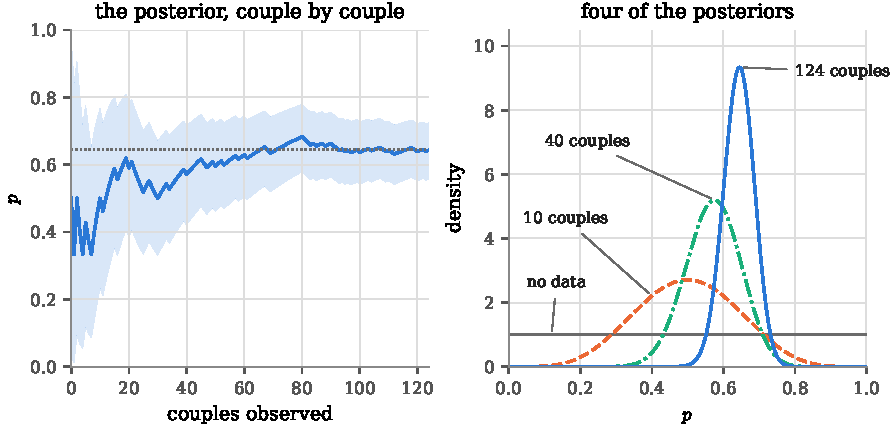
\includegraphics[width=\textwidth]{fig_bayes_sequential}
\caption{Kiss data, one couple at a time, flat prior. Left: posterior mean (blue), middle $95\%$ (shaded), $0.645$ (dotted). Right: posteriors after $0$ (gray), $10$ (orange, dashed), $40$ (aqua, dash-dot) and $124$ (blue) couples.}
\label{fig:bayessequential}
\end{figure}

\section{Summarizing the posterior}
\label{sec:bayes-summaries}

The posterior is the whole answer, and a report still needs numbers.
Three of them describe where it sits.

\begin{definition}[Posterior mean, median and mode]
\label{def:bayes-estimators}
The \textbf{posterior mean} $\E[\theta \mid \mathbf{x}] = \int_\Theta \theta\,\pi(\theta \mid \mathbf{x})\,\mathrm{d}\theta$ is also called the \textbf{Bayes estimator} for squared error. The \textbf{posterior median} is a median of the posterior distribution. The \textbf{maximum a posteriori} (MAP) estimate is a value of $\theta$ that maximizes $\pi(\theta \mid \mathbf{x})$, the mode of the posterior.
\end{definition}

\begin{inwords}
\textbf{In words.} The center of mass, the halfway point and the peak of the posterior. For a symmetric posterior with one peak they coincide; for a skewed one they spread out, usually in the order mode, median, mean, toward the long tail.
\par\smallskip
\textbf{For the kiss data.} With the flat prior the posterior is $\Betad(81, 45)$: mean $81/126 = 0.643$, median $0.644$, mode $80/124 = 0.645$, which is $\hat{p}$.
\end{inwords}

Why the mean?
Because it is the best single number under squared error, by the same identity as the bias--variance decomposition of \cref{ch:estimators}.

\begin{proposition}[The posterior mean minimizes squared error]
\label{prop:posterior-mean}
For a posterior with finite variance and every number $c$,
\[
\E\big[(\theta - c)^2 \mid \mathbf{x}\big] = \var(\theta \mid \mathbf{x}) + \big(\E[\theta \mid \mathbf{x}] - c\big)^2.
\]
So the posterior mean minimizes the posterior expected squared error, and the minimum is the posterior variance.
\end{proposition}

\optionalproof{The bias--variance identity of \cref{thm:bias-variance}, with the posterior in place of the sampling distribution and $c$ in place of the true value: the cross term averages to zero.}
\begin{proof}
Write $\bar\theta = \E[\theta \mid \mathbf{x}]$. Then $(\theta - c)^2 = (\theta - \bar\theta)^2 + 2(\theta - \bar\theta)(\bar\theta - c) + (\bar\theta - c)^2$. Take the posterior expectation of each term: the first gives $\var(\theta \mid \mathbf{x})$; in the second, $\bar\theta - c$ is a number and $\E[\theta - \bar\theta \mid \mathbf{x}] = 0$; the third is a number. The first term does not involve $c$, and the last is smallest, $0$, at $c = \bar\theta$.
\end{proof}

The same reasoning with absolute error picks the posterior median: \cref{prop:median-min}, applied to the posterior distribution, says the median minimizes $\E[\abs{\theta - c} \mid \mathbf{x}]$ (its hypotheses, a continuous density with a finite mean, hold for the Beta posteriors with both parameters above $1$ and for the Gamma and Gaussian posteriors here).
The mode answers a different question.
Taking logarithms,
\[
\log\pi(\theta \mid \mathbf{x}) = \ell_n(\theta) + \log\pi(\theta) - \log m(\mathbf{x}),
\]
so the MAP estimate maximizes the log-likelihood plus $\log\pi(\theta)$, which is very negative where the prior is small and so works as a penalty.
With a flat prior the penalty is constant and the MAP estimate is the maximum likelihood estimator; with a Gaussian prior $\Gauss(\mu_0, \sigma_0^2)$ it is $-(\theta - \mu_0)^2/(2\sigma_0^2)$ plus a constant, a quadratic penalty that pulls toward $\mu_0$ (in regression the same penalty is called ridge).

\begin{pitfall}[the MAP estimate depends on the parameterization]
The maximum likelihood estimator follows any one-to-one change of parameter (\cref{prop:mle-invariance}); the MAP estimate does not: a density changes shape when its variable is transformed. If $\psi = g(p)$ with $g$ increasing, then $\Pr(\psi \leq t) = \Pr(p \leq g^{-1}(t))$, and differentiating in $t$ shows that the density of $\psi$ is the density of $p$ times $\mathrm{d}p/\mathrm{d}\psi$.
With the flat prior, the MAP estimate of $p$ for the kiss data is $0.645$.
The log-odds $\psi = \log\big(p/(1 - p)\big)$ has posterior density $\pi(p \mid \mathbf{x})\,p(1 - p) \propto p^{81}(1 - p)^{45}$, written in terms of $p$, which peaks at $p = 81/126 = 0.643$ (\cref{ex:bayes-map}).
The two MAP estimates describe different values of $p$.
The posterior median follows every increasing change of parameter, since it is defined by probabilities.
\end{pitfall}

The posterior also predicts.
The probability that the next couple turns right, given the data, averages $p$ over the posterior:
\[
\Pr(X_{n+1} = 1 \mid \mathbf{x}) = \int_0^1 p\,\pi(p \mid \mathbf{x})\,\mathrm{d}p = \E[p \mid \mathbf{x}] = \frac{a + S}{a + b + n}.
\]
With the flat prior this is $(S + 1)/(n + 2)$, Laplace's rule of succession: $81/126 = 0.643$ for the kiss data, close to the plug-in $\hat{p} = 0.645$.
The two differ when data are few: after $3$ right turns in $3$ couples the plug-in answer is $1$, a certainty that a fourth will turn right, and Laplace's rule gives $0.8$.
Laplace's $0.8$ is the plug-in $1$ pulled toward the prior mean $\frac12$ by the two imaginary couples: $0.8 = \frac25 \times \frac12 + \frac35 \times 1$.

\section{Probabilities of intervals and of hypotheses}
\label{sec:bayes-hypotheses}

\Cref{ch:confidence-intervals} called `$\Pr(p \in [0.56, 0.73]) = 0.95$' a Bayesian statement and said this chapter would say what it costs.
The posterior gives such probabilities directly.
For the kiss data, $\Pr(0.56 \leq p \leq 0.73 \mid \text{data})$ is $0.955$ with the flat prior, $0.941$ with $\Betad(10, 10)$ and $0.835$ with the skeptic's prior.
The cost is the prior: the probability belongs to the prior and the data together, and a reader with a different prior gets a different number.
With the flat prior it comes out near the confidence level $0.95$ ($0.952$ for the plug-in interval $[0.561, 0.729]$ itself; rounding it out to $[0.56, 0.73]$ gives $0.955$), and \cref{sec:bayes-bvm} explains why.
The question \cref{ch:likelihood} could not answer, the probability that $p$ is between $0.6$ and $0.7$, now has an answer: $0.75$ with the flat prior.

A one-sided hypothesis gets a probability the same way.
With the flat prior, $\Pr(p \leq \frac12 \mid \text{data}) = 0.0006$, the same number as the one-sided $p$-value of \cref{ch:tests-foundations} by the Gaussian approximation (the exact Binomial $p$-value is $0.0008$; \cref{ex:bayes-tail} explains the near agreement).
The numbers agree; the questions do not.
The $p$-value is the probability of data this extreme if $p = \frac12$; the posterior probability is the probability that $p \leq \frac12$ given the data.

A point hypothesis such as $H_0: p = \frac12$ is different, and \cref{ch:tests-foundations} promised a different number for it.
Under a continuous prior a single value has probability $0$, before and after the data, so a prior that takes $H_0$ seriously must put a lump of probability on $p = \frac12$.
Take probability $\frac12$ on $p = \frac12$ and spread the other $\frac12$ uniformly over $(0, 1)$.
This prior has neither a density nor a PMF, so \cref{def:posterior} does not cover it, but Bayes' rule for the two events $H_0: p = \frac12$ and $H_1: p \neq \frac12$ does.
Write $m_0$ and $m_1$ for the probability of the data under $H_0$ and under $H_1$; then $m(\mathbf{x}) = m_0\Pr(H_0) + m_1\Pr(H_1)$, $\Pr(H_j \mid \mathbf{x}) = m_j\Pr(H_j)/m(\mathbf{x})$ for $j = 0, 1$, and dividing the two gives the odds form,
\[
\frac{\Pr(H_0 \mid \mathbf{x})}{\Pr(H_1 \mid \mathbf{x})} = \frac{m_0}{m_1} \cdot \frac{\Pr(H_0)}{\Pr(H_1)},
\]
where $m_0 = 2^{-124} = 4.7 \times 10^{-38}$ and $m_1 = \int_0^1 p^{80}(1 - p)^{44}\,\mathrm{d}p = 1.0 \times 10^{-36}$, the probability of the data averaged over the uniform prior: the area under the sequence likelihood that \cref{ch:likelihood} said meant nothing as an area, and that means something here.
The ratio $B_{01} = m_0/m_1$ is the \textbf{Bayes factor}; here it is $0.0465$, the prior odds are $1$, and so $\Pr(H_0 \mid \mathbf{x}) = 0.0465/1.0465 = 0.044$.
Among $1{,}000$ studies that saw $80$ right turns, in a world where no preference and a uniformly spread preference were equally likely beforehand, about $44$ had no preference.
The two-sided $p$-value was $0.0012$, about $36$ times smaller.
The data favor a preference by a factor of $1/B_{01} = 21$; the likelihood ratio of \cref{ch:wald-lrt}, $e^{10.60/2} = 200$, is about nine times larger, since it compares $H_0$ with the single best value $\hat{p}$, while the Bayes factor compares it with the average over every $p$, including values the data rule out.

The gap grows with $n$.
Keep the two-sided $p$-value at $0.0012$, so that the standardized statistic stays $3.23$, and let the number of couples grow, with the same prior:
\begin{center}
\small
\begin{tabular}{@{}lrrrrr@{}}
\toprule
couples $n$ & $124$ & $1{,}240$ & $12{,}400$ & $124{,}000$ & $1{,}240{,}000$ \\
right turns & $80$ & $677$ & $6{,}380$ & $62{,}569$ & $621{,}800$ \\
$\Pr(H_0 \mid \text{data})$ & $0.04$ & $0.13$ & $0.32$ & $0.60$ & $0.83$ \\
\bottomrule
\end{tabular}
\end{center}
At a fixed $p$-value, a larger sample is stronger evidence for the point null, since a true preference would have produced a larger standardized statistic in a larger sample.
Lindley (\textit{Biometrika}, 1957) pointed out this divergence, now called Lindley's paradox; Berger and Sellke (\textit{Journal of the American Statistical Association}, 1987) showed that, for a Gaussian mean, at a $p$-value of $0.05$ the posterior probability of a point null with prior probability $\frac12$ is at least $0.29$ for every prior on the alternative that is symmetric about the null value with a single peak there, and at least $0.128$ for every prior whatsoever.

\section{When the data outweigh the prior}
\label{sec:bayes-bvm}

The priors of \cref{fig:bayesbeta} disagree, and their posteriors disagree less.
With more data they would disagree less still.

\recall{The Law of Large Numbers (\cref{thm:wlln}): for i.i.d.\ random variables with mean $\mu$ and finite variance, $\bar{X}_n \convp \mu$. Chebyshev's inequality \toolkit{sec:math-inequalities}: $\Pr(\abs{Y - \E[Y]} \geq t) \leq \var(Y)/t^2$ for any random variable $Y$ with finite variance and any $t > 0$.}

\begin{theorem}[The prior washes out]
\label{thm:prior-washout}
Let $a, b > 0$, and let $\Xton$ be i.i.d.\ $\Bern(p^*)$, where $p^*$ is the fixed true value. For the posterior from the prior $\Betad(a, b)$, which depends on the data and is therefore random:
\begin{enumerate}[nosep]
\item the posterior mean converges to $p^*$ in probability;
\item for every $\varepsilon > 0$, the posterior probability $\Pr(\abs{p - p^*} < \varepsilon \mid X_1, \ldots, X_n)$ converges to $1$ in probability.
\end{enumerate}
\end{theorem}

\coreproof{The weight on the prior mean is $(a + b)/(a + b + n)$, which goes to $0$, and the sample proportion goes to $p^*$; the posterior variance is at most $1/(4n)$, so the posterior piles up at its mean.}
\begin{proof}
(1) Fix $\varepsilon > 0$, let $S = \sum_i X_i$, and write $\bar{p}_n$ for the posterior mean. By the weighted average of \cref{sec:bayes-beta}, $\bar{p}_n - S/n = w_n\big(a/(a + b) - S/n\big)$ with $w_n = (a + b)/(a + b + n)$, which is at most $w_n$ in absolute value since both $a/(a + b)$ and $S/n$ lie in $[0, 1]$. So $\abs{\bar{p}_n - p^*} \leq w_n + \abs{S/n - p^*}$. Once $w_n < \varepsilon/2$, the event $\abs{\bar{p}_n - p^*} \geq \varepsilon$ forces $\abs{S/n - p^*} \geq \varepsilon/2$, whose probability tends to $0$ by the Law of Large Numbers.

(2) Write $a_n = a + S$ and $b_n = b + n - S$. The posterior variance is $a_nb_n/\big((a_n + b_n)^2(a_n + b_n + 1)\big)$, and $a_nb_n \leq (a_n + b_n)^2/4$, so it is at most $1/\big(4(a + b + n + 1)\big)$. By Chebyshev's inequality applied to the posterior distribution, the posterior probability that $p$ is at least $\varepsilon/2$ from $\bar{p}_n$ is at most $c_n = 1/\big(\varepsilon^2(a + b + n + 1)\big)$. If $p$ is within $\varepsilon/2$ of $\bar{p}_n$ and $\bar{p}_n$ is within $\varepsilon/2$ of $p^*$, then $\abs{p - p^*} < \varepsilon$. So on the event $E_n$ that $\bar{p}_n$ is within $\varepsilon/2$ of $p^*$, $Y_n = \Pr(\abs{p - p^*} < \varepsilon \mid X_1, \ldots, X_n) \geq 1 - c_n$. Given $\eta > 0$, once $c_n < \eta$ the event $Y_n \leq 1 - \eta$ lies outside $E_n$, so $\Pr(\abs{Y_n - 1} \geq \eta) \leq \Pr(E_n^c) \to 0$ by (1).
\end{proof}

\Cref{fig:bayesbvm} draws it.
At $124$ couples the three posterior means of \cref{fig:bayesbeta} spread over $0.048$, about one posterior standard deviation; with ten times as many couples in the same proportion, $800$ of $1{,}240$, they spread over $0.007$, half a standard deviation of $0.014$, and the three posteriors nearly coincide with a single Gaussian centered at $\hat{p}$ with the standard error $\sqrt{\hat{p}(1 - \hat{p})/n}$ of \cref{ch:confidence-intervals}.
That Gaussian is the general limit.

\begin{figure}[htbp]
\centering
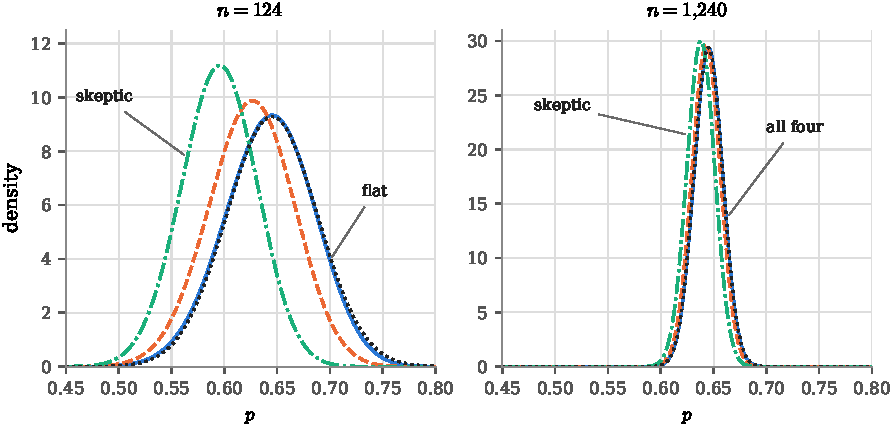
\includegraphics[width=\textwidth]{fig_bayes_bvm}
\caption{Posteriors from the flat prior (blue), $\Betad(10, 10)$ (orange, dashed) and the skeptic's $\Betad(33, 33)$ (aqua, dash-dot), with $\Gauss\big(\hat{p}, \hat{p}(1 - \hat{p})/n\big)$ (black, dotted). Left: $80$ right turns in $124$ couples. Right: $800$ in $1{,}240$.}
\label{fig:bayesbvm}
\end{figure}

\recall{Asymptotic normality of the maximum likelihood estimator (\cref{thm:mle-normal}): under the regularity conditions of \cref{sec:mle-regularity}, with $\theta^*$ in the interior of $\Theta$ and $I(\theta^*) > 0$, $\sqrt{n}(\hat{\theta}_n - \theta^*) \convd \Gauss\big(0, 1/I(\theta^*)\big)$.}

\begin{theorem}[Bernstein--von Mises]
\label{thm:bvm}
Let $\Xton \iid \Pr_{\theta^*}$ in a model satisfying the regularity conditions of \cref{sec:mle-regularity}, with $\theta^*$ in the interior of $\Theta$ and $I(\theta^*) > 0$, let $\hat{\theta}_n$ be the maximum likelihood estimator, and suppose the data separate $\theta^*$ from distant values: for every $\varepsilon > 0$ there is a $\delta > 0$ such that, with probability tending to $1$, $\frac1n\big(\ell_n(\theta) - \ell_n(\theta^*)\big) \leq -\delta$ for every $\theta$ with $\abs{\theta - \theta^*} \geq \varepsilon$ (this holds for the models of this chapter). Let the prior have a density that is continuous and positive at $\theta^*$. Then the total variation distance (\cref{ch:distances}) between the posterior distribution of $\sqrt{n}(\theta - \hat{\theta}_n)$, with $\theta$ random and $\hat{\theta}_n$ the number computed from the data, and $\Gauss\big(0, 1/I(\theta^*)\big)$ converges to $0$ in probability under $\Pr_{\theta^*}$. Informally, for large $n$ the posterior is approximately $\Gauss\big(\hat{\theta}_n, 1/(nI(\hat{\theta}_n))\big)$, for every such prior.
\end{theorem}

This theorem is stated without proof; its proof needs more than this book develops. It is named for Bernstein (1917) and von Mises (1931), though Laplace had already found it for a proportion with a flat prior; its modern form is due to Le Cam (1953).
The reason it holds is visible in the log-posterior, $\ell_n(\theta) + \log\pi(\theta)$ up to a constant.
The log-likelihood grows with $n$, and near its peak it is a parabola whose curvature is about $nI(\theta^*)$ (\cref{ch:mle-properties}); the log-prior stays the same size, and over the width of about $1/\sqrt{nI(\theta^*)}$ where the likelihood matters it is nearly constant, which is why the prior must be continuous and positive at $\theta^*$.
So for large $n$ the log-posterior is that parabola, and a density whose logarithm is a parabola is Gaussian.
\Cref{thm:mle-normal} and \cref{thm:bvm} read the same parabola from two sides: the first describes how the estimate $\hat{\theta}_n$ scatters around the fixed $\theta^*$, the second how the posterior spreads around the fixed $\hat{\theta}_n$, with the same variance $1/(nI)$.
That is why the flat-prior probability of the $95\%$ confidence interval came out near $0.95$, and why Bayesian and frequentist intervals nearly coincide in large samples.

\section{What comes next}
\label{sec:bayes-next}

Every posterior in this chapter came from a prior someone chose.
\Cref{ch:jeffreys} asks what to use when there is nothing to put in a prior: flat priors and their dependence on the parameterization, improper priors, whose density has an infinite integral and so cannot be rescaled to integrate to $1$, and Jeffreys' prior, built from the Fisher information so that it does not depend on the parameterization.
It then builds Bayesian confidence regions, intervals with a stated posterior probability, and compares them with the intervals of \cref{ch:confidence-intervals}, using the Bernstein--von Mises theorem.

\section{Summary}
\label{sec:bayes-summary}

\begin{itemize}[nosep]
\item Bayesian model: a prior $\pi$ on $\Theta$, and the data i.i.d.\ $\Pr_\theta$ given $\theta$. Posterior: $\pi(\theta \mid \mathbf{x}) \propto L_n(\mathbf{x}; \theta)\pi(\theta)$, rescaled by the marginal likelihood $m(\mathbf{x})$. A parameter value with prior probability $0$ keeps posterior probability $0$.
\item Grid: nine candidate values of the kiss proportion; the posterior puts $0.58$ on $0.6$ and $0.42$ on $0.7$.
\item Conjugate pairs: Beta prior and Bernoulli data give $\Betad(a + S, b + n - S)$; Gamma and exponential give $\Gammad(\alpha + n, \beta + \sum T_i)$; Gaussian and Gaussian give precisions that add. The prior acts as imaginary data: $a + b$ couples, $\alpha$ waits, $\sigma^2/\sigma_0^2$ observations. Kiss posterior means: $0.643$ (flat), $0.625$ ($\Betad(10, 10)$, the shrinkage estimator), $0.595$ (skeptic).
\item Updating in stages, or one observation at a time in any order, gives the same posterior.
\item Posterior mean: best under squared error, with the posterior variance as its error. Median: best under absolute error. MAP: maximizes the log-likelihood plus $\log\pi$, depends on the parameterization. The predictive probability of the next success is the posterior mean, Laplace's $(S + 1)/(n + 2)$ with a flat prior.
\item Interval and one-sided probabilities depend on the prior ($0.955$, $0.941$, $0.835$ for $[0.56, 0.73]$). A point null needs prior mass; for the kiss data its posterior probability is $0.044$ against a $p$-value of $0.0012$, and at a fixed $p$-value it grows with $n$ (Lindley).
\item The prior washes out: with Beta priors the posterior concentrates at $p^*$; in general (Bernstein--von Mises) the posterior is approximately $\Gauss\big(\hat{\theta}_n, 1/(nI(\hat{\theta}_n))\big)$.
\end{itemize}

\section{Exercises}
\label{sec:bayes-exercises}

\begin{exercise}
\label{ex:bayes-beta-moments}
Let $P \sim \Betad(a, b)$. (a) Using $B(a, b) = \Gamma(a)\Gamma(b)/\Gamma(a + b)$ and $\Gamma(x + 1) = x\Gamma(x)$, show that $\E[P] = a/(a + b)$ and $\E[P^2] = a(a + 1)/\big((a + b)(a + b + 1)\big)$, and deduce the variance. (b) Show that for $a, b > 1$ the density is largest at $(a - 1)/(a + b - 2)$.
\end{exercise}
\begin{solution}
(a) $\E[P] = \int_0^1 p \cdot p^{a-1}(1 - p)^{b-1}\,\mathrm{d}p/B(a, b) = B(a + 1, b)/B(a, b) = \frac{\Gamma(a + 1)\Gamma(a + b)}{\Gamma(a)\Gamma(a + b + 1)} = \frac{a}{a + b}$. Likewise $\E[P^2] = B(a + 2, b)/B(a, b) = \frac{a(a + 1)}{(a + b)(a + b + 1)}$. So $\var(P) = \frac{a(a + 1)}{(a + b)(a + b + 1)} - \frac{a^2}{(a + b)^2} = \frac{a\big[(a + 1)(a + b) - a(a + b + 1)\big]}{(a + b)^2(a + b + 1)} = \frac{ab}{(a + b)^2(a + b + 1)}$, since $(a + 1)(a + b) - a(a + b + 1) = b$. (b) The log-density is $(a - 1)\log p + (b - 1)\log(1 - p)$ plus a constant, with derivative $(a - 1)/p - (b - 1)/(1 - p)$, which is $0$ at $p = (a - 1)/(a + b - 2)$; the second derivative $-(a - 1)/p^2 - (b - 1)/(1 - p)^2$ is negative, so this is the maximum.
\end{solution}

\begin{exercise}
\label{ex:bayes-flat-marginal}
(a) With the flat prior on $p$, show that the number of successes $S$ in $n$ Bernoulli trials has $\Pr(S = s) = 1/(n + 1)$ for every $s = 0, 1, \ldots, n$, using $B(s + 1, n - s + 1) = s!\,(n - s)!/(n + 1)!$. (b) For the kiss data, compute $m_1 = \int_0^1 p^{80}(1 - p)^{44}\,\mathrm{d}p$ in terms of a binomial coefficient, and check the Bayes factor $B_{01} = 0.0465$ of \cref{sec:bayes-hypotheses}, given that $\binom{124}{80}2^{-124} = 0.000372$.
\end{exercise}
\begin{solution}
(a) $\Pr(S = s) = \int_0^1 \binom{n}{s}p^s(1 - p)^{n-s}\,\mathrm{d}p = \binom{n}{s}B(s + 1, n - s + 1) = \frac{n!}{s!\,(n - s)!}\cdot\frac{s!\,(n - s)!}{(n + 1)!} = \frac{1}{n + 1}$. Before any data, every count is equally likely, which is how Bayes himself chose the flat prior in 1763. (b) $m_1 = B(81, 45) = 80!\,44!/125! = 1/\big(125\binom{124}{80}\big)$, so $B_{01} = 2^{-124}/m_1 = 125\binom{124}{80}2^{-124} = 125 \times 0.000372 = 0.0465$.
\end{solution}

\begin{exercise}
\label{ex:bayes-drug}
In the drug trial of \cref{ch:kiss}, earlier studies showed the drug to be about $80\%$ effective. (a) Express this as a $\Betad(40, 10)$ prior: what is its mean, and how many patients does it count as? (b) After $78$ cures in $100$ patients, find the posterior, its mean and its standard deviation, and the weight on the prior mean. (c) Compute $\Pr(p > 0.7 \mid \text{data})$ approximately with a Gaussian approximation to the posterior.
\end{exercise}
\begin{solution}
(a) Mean $40/50 = 0.8$; it counts as $50$ patients, $40$ cured. (b) $\Betad(118, 32)$: mean $118/150 = 0.787$, standard deviation $\sqrt{118 \times 32/(150^2 \times 151)} = 0.033$; the weight on the prior mean is $50/150 = \frac13$, and $0.787 = \frac13 \times 0.8 + \frac23 \times 0.78$. (c) $\Pr(p > 0.7) \approx 1 - \Phi\big((0.7 - 0.787)/0.033\big) = 1 - \Phi(-2.6) = 0.995$ (the exact Beta value is $0.992$).
\end{solution}

\begin{exercise}
\label{ex:bayes-siblings}
(a) Show that the Gamma family is conjugate for Poisson data: if $\lambda \sim \Gammad(\alpha, \beta)$ and, given $\lambda$, $\Xton \iid \Pois(\lambda)$, the posterior is $\Gammad(\alpha + \sum_i X_i, \beta + n)$. (b) In the siblings data of \cref{ch:models}, the $24$ values of $X - 1$ add up to $24$. With the prior $\Gammad(2, 2)$, find the posterior mean and standard deviation of $\lambda$ and compare with the maximum likelihood estimate.
\end{exercise}
\begin{solution}
(a) $\pi(\lambda \mid \mathbf{x}) \propto \prod_i e^{-\lambda}\lambda^{x_i} \cdot \lambda^{\alpha - 1}e^{-\beta\lambda} = \lambda^{\alpha + \sum x_i - 1}e^{-(\beta + n)\lambda}$, the shape of $\Gammad(\alpha + \sum x_i, \beta + n)$. (b) $\Gammad(26, 26)$: mean $1.0$, standard deviation $\sqrt{26}/26 = 0.196$. The maximum likelihood estimate is the sample mean, $1.0$; the prior, with mean $1$ and worth $2$ observations, agrees with the data and only narrows the posterior.
\end{solution}

\begin{exercise}
\label{ex:bayes-geometric}
Let $X_1, \ldots, X_n$ be i.i.d.\ geometric given $p$, with $\Pr(X = x) = (1 - p)^{x-1}p$ for $x = 1, 2, \ldots$ (the trial on which the first success occurs), and let $p \sim \Betad(a, b)$. Find the posterior and the posterior mean.
\end{exercise}
\begin{solution}
$\pi(p \mid \mathbf{x}) \propto \prod_i(1 - p)^{x_i - 1}p \cdot p^{a-1}(1 - p)^{b-1} = p^{a + n - 1}(1 - p)^{b + \sum x_i - n - 1}$, so the posterior is $\Betad\big(a + n, b + \sum_i x_i - n\big)$, with mean $(a + n)/(a + b + \sum_i x_i)$. The prior again counts as data: $a$ successes and $b$ failures.
\end{solution}

\begin{exercise}
\label{ex:bayes-invgamma}
Let $\Xton \iid \Gauss(0, v)$ given $v$, and give $v$ the Inverse Gamma prior with density $\pi(v) = \frac{b^a}{\Gamma(a)}v^{-a-1}e^{-b/v}$, $v > 0$, whose mean is $b/(a - 1)$ for $a > 1$. (a) Show that the posterior is Inverse Gamma with parameters $a + n/2$ and $b + \frac12\sum_i X_i^2$. (b) Find the posterior mean and its limit as $a$ and $b$ tend to $0$ (for $n \geq 3$). Is it the maximum likelihood estimate $\frac1n\sum_i X_i^2$?
\end{exercise}
\begin{solution}
(a) $\pi(v \mid \mathbf{x}) \propto \prod_i v^{-1/2}e^{-x_i^2/(2v)} \cdot v^{-a-1}e^{-b/v} = v^{-(a + n/2) - 1}e^{-(b + \sum x_i^2/2)/v}$, the shape of the Inverse Gamma with parameters $a + n/2$ and $b + \frac12\sum_i x_i^2$. (b) The posterior mean is $\big(b + \frac12\sum_i x_i^2\big)/(a + n/2 - 1)$, which tends to $\sum_i x_i^2/(n - 2)$, not the maximum likelihood estimate $\frac1n\sum_i x_i^2$. (The posterior mode, $\big(b + \frac12\sum_i x_i^2\big)/(a + n/2 + 1)$, tends to $\sum_i x_i^2/(n + 2)$; neither summary of this posterior is the maximum likelihood estimate.)
\end{solution}

\begin{exercise}
\label{ex:bayes-tail}
(a) Show that if $S$ of $n$ trials are successes and the prior is flat, then $\Pr(p \leq x \mid \text{data}) = \Pr\big(\Bin(n + 1, x) \geq S + 1\big)$ for $0 < x < 1$. (Hint: the $(S + 1)$th smallest of $n + 1$ independent $\Unif(0, 1)$ variables has the $\Betad(S + 1, n - S + 1)$ distribution.) (b) For the kiss data, compare $\Pr(p \leq \frac12 \mid \text{data}) = \Pr(\Bin(125, \frac12) \geq 81)$ with the exact one-sided $p$-value $\Pr(\Bin(124, \frac12) \geq 80)$, which are $0.00060$ and $0.00078$.
\end{exercise}
\begin{solution}
(a) The posterior is $\Betad(S + 1, n - S + 1)$, the distribution of the $(S + 1)$th smallest of $n + 1$ independent uniforms, whose density is $\frac{(n + 1)!}{S!\,(n - S)!}u^S(1 - u)^{n - S}$. That order statistic is at most $x$ exactly when at least $S + 1$ of the $n + 1$ uniforms are at most $x$, and the number of uniforms at most $x$ is $\Bin(n + 1, x)$. (b) The posterior probability uses one more trial and one more success than the $p$-value: $\Pr(\Bin(125, \frac12) \geq 81)$ against $\Pr(\Bin(124, \frac12) \geq 80)$. The two tail probabilities are of the same size, $0.00060$ and $0.00078$, which is why the posterior probability and the one-sided $p$-value nearly agree, though they answer different questions.
\end{solution}

\begin{exercise}
\label{ex:bayes-map}
With the flat prior on $p$ and the kiss data, (a) find the posterior density of the log-odds $\psi = \log\big(p/(1 - p)\big)$, using $\mathrm{d}p/\mathrm{d}\psi = p(1 - p)$, and show that it peaks where $p = 81/126$; (b) explain why the MAP estimate of $\psi$, transformed back, is not the MAP estimate of $p$, while the posterior median of $\psi$, transformed back, is the posterior median of $p$.
\end{exercise}
\begin{solution}
(a) A density of $p$ becomes a density of $\psi$ when multiplied by $\mathrm{d}p/\mathrm{d}\psi = p(1 - p)$, so the posterior of $\psi$ is proportional to $p^{80}(1 - p)^{44}\cdot p(1 - p) = p^{81}(1 - p)^{45}$, written in terms of $p$. As $p$ increases with $\psi$, this is largest where $p^{81}(1 - p)^{45}$ is, at $p = 81/126 = 0.643$, that is $\psi = \log(81/45) = 0.588$. (b) The factor $p(1 - p)$ changes where the density peaks, so the modes of the two densities correspond to different values of $p$: $0.645$ and $0.643$. The median is defined by probabilities, $\Pr(p \leq m) = \frac12$, and an increasing map preserves them: $\Pr(\psi \leq \log(m/(1 - m))) = \Pr(p \leq m) = \frac12$.
\end{solution}

\begin{exercise}
\label{ex:bayes-predictive}
With the flat prior and the kiss data, find the probability that the next $10$ couples all turn right, $\E[p^{10} \mid \text{data}]$, as a product of $10$ fractions, and compare it with the plug-in answer $\hat{p}^{10}$.
\end{exercise}
\begin{solution}
Given $p$ the probability is $p^{10}$, so the predictive probability is $\E[p^{10} \mid \text{data}] = B(91, 45)/B(81, 45) = \prod_{j=0}^{9}\frac{81 + j}{126 + j} = 0.0145$, against $0.645^{10} = 0.0125$. By Jensen's inequality \toolkit{sec:math-convex}, $\E[p^{10} \mid \text{data}] \geq (\E[p \mid \text{data}])^{10} = 0.643^{10} = 0.0121$: values of $p$ above the mean raise $p^{10}$ more than values below it lower it. The bound alone is below $\hat{p}^{10}$, since the posterior mean is below $\hat{p}$; the exact $0.0145$ shows that the spread of the posterior adds enough to pass $\hat{p}^{10}$.
\end{solution}

\chapter{Jeffreys Priors and Bayesian Intervals}
\label{ch:jeffreys}

\begin{chaptergoals}
\begin{itemize}[nosep]
\item What a prior for `knowing nothing' can be, and why the flat prior gives a different answer on each scale a parameter can be written on: the proportion $p$ against its log-odds, a rate against a mean wait.
\item Improper priors, whose densities have an infinite integral: when they still give a proper posterior, when they give none, and why they cannot be the prior for the parameter that a point null fixes.
\item Jeffreys' prior, built from the Fisher information so that changing the parameterization changes nothing: $\Betad(\frac12, \frac12)$ for the kiss data, $1/\lambda$ for the subway rate, $1/\sigma$ for a scale. Why it puts equal mass on what the data can tell apart.
\item Bayesian confidence regions, equal-tailed and highest-density, and what their $95\%$ means. When they coincide with the intervals of \cref{ch:confidence-intervals,ch:t-test} exactly (the subway's exact interval, the $t$-interval) and when only for large $n$ (Bernstein--von Mises).
\end{itemize}
\Cref{ch:bayes-intro} turned a prior and the likelihood into a posterior. This chapter asks which prior to use when there is nothing to put in one, and what the posterior's intervals mean.
\end{chaptergoals}

\section{A prior for knowing nothing}
\label{sec:jeff-flat}

Every posterior in \cref{ch:bayes-intro} started from a prior somebody chose: a timetable's promise for the subway, a regional average for the wind turbine, a skeptic's $90\%$ belief for the kiss data.
Often there is nothing of the sort to write down, or the point of the analysis is to report what the data say on their own.
The oldest answer is to give every value of the parameter the same density.
Bayes (1763) did this for a proportion, and Laplace made it a rule, later called the principle of insufficient reason: with no reason to prefer one value, prefer none.
For the kiss data the flat prior gives the posterior $\Betad(81, 45)$ of \cref{thm:beta-bernoulli}, with mean $0.643$ and middle $95\%$ from $0.558$ to $0.724$.

The trouble is that `the same density for every value' depends on how the values are written.
The kiss proportion $p$ can just as well be described by its log-odds, $\psi = \log(p/(1-p))$, the scale on which logistic regression works (\cref{ch:glm-links}), and someone who knows nothing about $p$ knows nothing about $\psi$ either.
But a flat density for $p$ is not flat for $\psi$.
To find the density of $\psi$, write its CDF and differentiate \toolkit{sec:math-density}: for a strictly increasing smooth map $\psi = g(p)$, $\Pr(\psi \leq u) = \Pr(p \leq g^{-1}(u))$, and the derivative in $u$ is the density of $p$ at $g^{-1}(u)$ times the derivative of $g^{-1}$.
In general, for a smooth one-to-one map $\varphi = g(\theta)$,
\begin{equation}
\label{eq:jeff-change}
\pi_\varphi(\varphi) = \pi_\theta(\theta)\,\abs*{\frac{\mathrm{d}\theta}{\mathrm{d}\varphi}}, \qquad \theta = g^{-1}(\varphi),
\end{equation}
where the absolute value covers decreasing maps.
For the log-odds, $p = e^\psi/(1 + e^\psi)$ and $\mathrm{d}p/\mathrm{d}\psi = p(1-p)$, so the flat prior on $p$ becomes the density $p(1-p) = e^\psi/(1 + e^\psi)^2$ on $\psi$: the logistic density, peaked at $\psi = 0$, which is $p = \frac12$.
It is far from ignorant about $\psi$: it puts probability $0.90$ on $\abs{\psi} \leq 2.94$, which is the event $0.05 \leq p \leq 0.95$.
Run the other way, a flat prior on $\psi$ becomes the density $1/(p(1-p))$ on $p$, which piles up at $0$ and at $1$.

\Cref{fig:jeffscales} draws this, together with the prior this chapter ends up recommending.
On the left, on the scale of $p$, the flat prior is the blue line.
On the right, on the scale of $\psi$, the same prior is the blue bell, while the flat rule applied to $\psi$ directly gives the gray line: two people who both claim to know nothing about the kiss data, one thinking in $p$ and one in $\psi$, start from different priors and end with different posteriors.
The orange curves are Jeffreys' prior of \cref{sec:jeff-prior}, a U on the left and a wider bell on the right.
The orange dots on the right were computed on $\psi$ directly, by Jeffreys' rule, and they land on the orange curve: that rule gives one answer on both scales.

\begin{figure}[htbp]
\centering
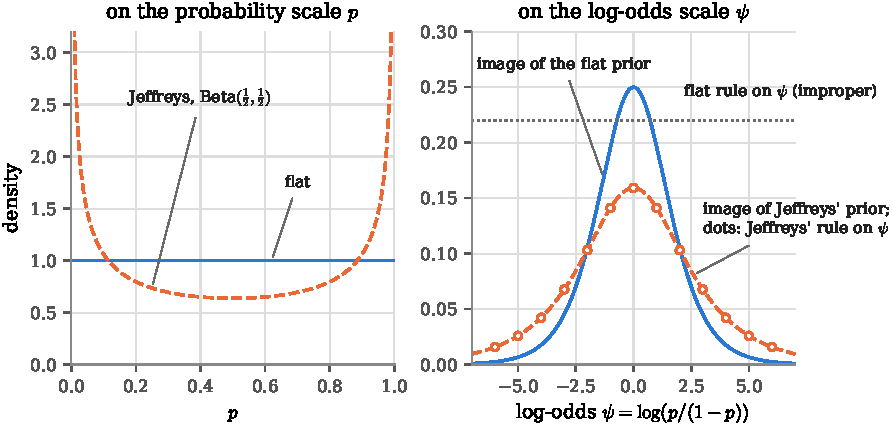
\includegraphics[width=\textwidth]{fig_jeffreys_scales}
\caption{Two priors for the kiss proportion. Left, on $p$: flat (blue) and Jeffreys' $\Betad(\frac12, \frac12)$ (orange, dashed). Right, on the log-odds $\psi$: their images (same colors), the flat rule on $\psi$ (gray dotted, height arbitrary) and Jeffreys' rule on $\psi$ (orange dots).}
\label{fig:jeffscales}
\end{figure}

The subway gives a second example.
Its rate $\lambda$, in trains per minute, and its mean wait $\beta = 1/\lambda$, in minutes per train, are two descriptions of one parameter.
A flat prior on $\lambda$ is the density $1$ on $(0, \infty)$; a flat prior on $\beta$ becomes, by \cref{eq:jeff-change} with $\abs{\mathrm{d}\beta/\mathrm{d}\lambda} = 1/\lambda^2$, the density $1/\lambda^2$ on $\lambda$.
The $64$ waits total $398.7$ minutes, so the likelihood is $\lambda^{64}e^{-398.7\lambda}$ (\cref{ch:likelihood}), and the two posteriors are $\Gammad(65, 398.7)$ and $\Gammad(63, 398.7)$, with means $0.163$ and $0.158$ trains per minute and middle $95\%$ intervals $[0.126, 0.205]$ and $[0.121, 0.199]$.
Neither prior has a finite integral, which \cref{sec:jeff-improper} takes up, yet both posteriors are ordinary Gamma distributions.
At $n = 64$ the two posterior means differ by a quarter of a posterior standard deviation ($0.005$ against $0.020$), a difference produced by nothing but the choice between `rate' and `wait'.

\begin{pitfall}[`uninformative' is not a property of a prior alone]
A prior that is flat for $p$ is informative about $\psi$, about $p^2$ and about every other nonlinear function of $p$, and no density is flat on every scale at once.
`I used a flat prior' says nothing until it says flat \textit{in what}.
\Cref{ch:bayes-intro} met the same problem from the other side: the posterior mode moved from $0.645$ to $0.643$ when the kiss data were described by their log-odds (\cref{ex:bayes-map}) because a mode is where a density peaks, and densities change under a change of variables.
\end{pitfall}

\section{Improper priors}
\label{sec:jeff-improper}

The flat prior on the subway rate gives every $\lambda > 0$ the same density, and $\int_0^\infty 1\,\mathrm{d}\lambda = \infty$, so no rescaling makes it a probability distribution and \cref{def:posterior}, which asks for one, does not cover it.
Yet the posterior it produced, $\Gammad(65, 398.7)$, is an ordinary distribution.
Bayes' formula uses the prior only through the product $L_n\pi$ and its integral, and those can be finite when the integral of $\pi$ is not.

\begin{definition}[Improper prior]
\label{def:improper-prior}
An \textbf{improper prior} on $\Theta$ is a nonnegative function $\pi$ on $\Theta$ with $\int_\Theta \pi(\theta)\,\mathrm{d}\theta = \infty$. For data $\mathbf{x}$ with
\[
0 < m(\mathbf{x}) = \int_\Theta L_n(\mathbf{x}; t)\,\pi(t)\,\mathrm{d}t < \infty,
\]
its \textbf{posterior} is $\pi(\theta \mid \mathbf{x}) = L_n(\mathbf{x}; \theta)\,\pi(\theta)/m(\mathbf{x})$, a probability density on $\Theta$. A prior with a finite integral, rescaled to integrate to $1$, is called \textbf{proper}.
\end{definition}

\begin{inwords}
\textbf{In words.} An improper prior is a weighting of the parameter values whose total weight is infinite, so it is not a distribution. It is used only through Bayes' formula: when likelihood times prior has a finite integral, the posterior is a genuine distribution, and when it does not, there is no posterior. Multiplying an improper prior by a constant changes nothing, since the constant cancels.
\par\smallskip
\textbf{For the kiss data.} The flat prior on the log-odds, $\pi(p) = 1/(p(1-p))$ on $(0, 1)$, is improper: its integral diverges at both ends. Times the likelihood $p^{80}(1-p)^{44}$ it gives $p^{79}(1-p)^{43}$, which has a finite integral, so the posterior is $\Betad(80, 44)$, with mean $80/124 = 0.645$, the sample proportion.
\end{inwords}

This prior is known as Haldane's prior, after J. B. S. Haldane (\textit{Proceedings of the Cambridge Philosophical Society}, 1932).
Where improper priors come from is easiest to see for a Gaussian mean with $\sigma$ known.
There \cref{prop:normal-normal} turned the prior $\Gauss(\mu_0, \sigma_0^2)$ into a posterior with precision $1/\sigma_0^2 + n/\sigma^2$, whose mean is the precision-weighted average of $\mu_0$ and $\bar{x}$.

\begin{intuition}[an improper prior is the limit of wider and wider proper ones]
Let the prior's standard deviation $\sigma_0$ grow.
The prior flattens toward the constant $0$, which is no density at all, but the posterior settles down: its precision tends to $n/\sigma^2$ and its mean to $\bar{x}$, so the posterior tends to $\Gauss(\bar{x}, \sigma^2/n)$.
That limit is what the improper flat prior $\pi(\mu) = 1$ gives in one step, since the likelihood is $\exp(-n(\mu - \bar{x})^2/(2\sigma^2))$ times a factor free of $\mu$, already a Gaussian shape in $\mu$.
For the wind turbine with $\sigma = 4.7$ treated as known, the prior centered at $11$ with $\sigma_0 = 2$ gave posterior mean $13.26$; with $\sigma_0 = 10$ the mean is $14.24$, and in the limit it is $\bar{x} = 14.3$, with standard deviation $4.7/\sqrt{12} = 1.36$.
An improper prior is shorthand for `a prior so wide that its exact width does not matter'.
\end{intuition}

The condition $m(\mathbf{x}) < \infty$ in \cref{def:improper-prior} is the price of that shorthand, and it can fail.

\begin{pitfall}[an improper prior can give no posterior]
Under Haldane's prior, suppose all $n$ couples had turned right.
Then $L_n\pi = p^{n-1}(1-p)^{-1}$, whose integral diverges at $p = 1$, and there is no posterior at all.
The formula still produces a function, and normalizing it numerically on a grid even produces a picture, but the picture depends on where the grid stops.
With a proper prior and discrete data this cannot happen, since then $m(\mathbf{x}) \leq 1$.
The results of \cref{ch:bayes-intro} that assume a prior distribution, \cref{thm:bvm} among them, do not apply as stated to an improper prior; for the improper priors of this chapter the Gaussian limit can be checked directly, since their posteriors are Gamma, Beta, Gaussian and $t$ distributions.
\end{pitfall}

Estimation and intervals tolerate improper priors because the arbitrary constant in front of the prior cancels between numerator and denominator.
One calculation of \cref{ch:bayes-intro} has no denominator to cancel it.

\begin{pitfall}[no improper prior for the parameter a point null fixes]
\Cref{sec:bayes-hypotheses} compared $H_0: p = \frac12$ with $H_1: p \neq \frac12$ through the Bayes factor $B_{01} = m_0/m_1$, where $m_1$ averages the likelihood over the prior on the alternative.
If that prior is improper, it is defined only up to a constant $c$, and $c$ multiplies $m_1$ but not $m_0$, which is computed at the single value $p = \frac12$: the Bayes factor, and $\Pr(H_0 \mid \mathbf{x})$ with it, can be made anything.
With Haldane's prior on the alternative, for instance, $B_{01}$ is $0.011$ for $c = 1$ and $0.000011$ for $c = 1{,}000$ (\cref{ex:jeff-bayes-factor}).
For testing, Jeffreys himself used proper priors for the parameter under test, such as a Cauchy prior for a Gaussian mean, and kept the improper $1/\sigma$ only for the $\sigma$ that both hypotheses share, whose constant cancels between $m_0$ and $m_1$.
\end{pitfall}

\section{Jeffreys' prior}
\label{sec:jeff-prior}

The flat prior failed because `constant density' is a rule that produces a different prior on each scale it is applied to.
Harold Jeffreys (\textit{Proceedings of the Royal Society A}, 1946) asked for a rule that does not: apply it on the scale of $\theta$ and carry the result to $\varphi = g(\theta)$ by \cref{eq:jeff-change}, or apply it on the scale of $\varphi$ directly, and get the same prior either way.
A fixed formula in $\theta$ cannot do this, since it ignores the factor $\abs{\mathrm{d}\theta/\mathrm{d}\varphi}$ that every change of variables puts on a density.
The rule has to be built from something attached to the model that changes with the parameterization in step with densities, and the Fisher information is such a thing.

\recall{The Fisher information of one observation (\cref{def:fisher}, \cref{thm:fisher-curvature}): for a model satisfying the regularity conditions of \cref{sec:mle-regularity}, $I(\theta) = \E_\theta[\ell'(\theta)^2] = -\E_\theta[\ell''(\theta)]$, where $\ell$ is the log-likelihood of one observation. A large $I(\theta)$ means one observation pins $\theta$ down well: the maximum likelihood estimator has asymptotic variance $1/I(\theta)$, so its standard error is about $1/\sqrt{nI(\theta)}$ (\cref{thm:mle-normal}).}

\begin{lemma}[Fisher information under a change of parameter]
\label{lem:fisher-reparam}
Let $\varphi = g(\theta)$ with $g$ smooth and one-to-one and $g' \neq 0$, and write $I_\theta$ and $I_\varphi$ for the Fisher information of one observation in the two parameterizations. Then
\[
I_\varphi(\varphi) = I_\theta(\theta)\Big(\frac{\mathrm{d}\theta}{\mathrm{d}\varphi}\Big)^2, \qquad \theta = g^{-1}(\varphi).
\]
\end{lemma}

\optionalproof{By the chain rule the score in $\varphi$ is the score in $\theta$ times the number $\mathrm{d}\theta/\mathrm{d}\varphi$, and a constant factor comes out of a variance squared.}
\begin{proof}
The model is the same, only the labels of its members change: the observation's density at the member labeled $\varphi$ is $p_{g^{-1}(\varphi)}(x)$. So the log-likelihood in $\varphi$ is $\tilde{\ell}(\varphi) = \ell(g^{-1}(\varphi))$, and by the chain rule $\tilde{\ell}'(\varphi) = \ell'(\theta)\,\mathrm{d}\theta/\mathrm{d}\varphi$ with $\theta = g^{-1}(\varphi)$. The factor $\mathrm{d}\theta/\mathrm{d}\varphi$ is a number, not a random variable, so $\var(\tilde{\ell}'(\varphi)) = (\mathrm{d}\theta/\mathrm{d}\varphi)^2\var(\ell'(\theta))$, which is the claim.
\end{proof}

\Cref{ex:mle-reparam} checked the lemma for the subway: $I = 1/\lambda^2$ for the rate and $1/\beta^2$ for the mean wait.
Which function of the information should the prior be?
Try a power, $\pi(\theta) \propto I_\theta(\theta)^a$.
Applied on the scale of $\theta$ and carried to $\varphi$ by \cref{eq:jeff-change}, it gives $I_\theta(\theta)^a\abs{\mathrm{d}\theta/\mathrm{d}\varphi}$.
Applied on the scale of $\varphi$ directly, it gives, by \cref{lem:fisher-reparam}, $I_\varphi(\varphi)^a = I_\theta(\theta)^a\abs{\mathrm{d}\theta/\mathrm{d}\varphi}^{2a}$.
The two are proportional for every change of variables only if $\abs{\mathrm{d}\theta/\mathrm{d}\varphi}^{2a - 1}$ is constant whatever $g$ is, and that forces $2a = 1$.

\begin{definition}[Jeffreys' prior]
\label{def:jeffreys}
For a one-parameter model with Fisher information $I(\theta)$, \textbf{Jeffreys' prior} is
\[
\pi_J(\theta) \propto \sqrt{I(\theta)},
\]
proper or improper according to whether $\int_\Theta \sqrt{I(\theta)}\,\mathrm{d}\theta$ is finite. For $\theta \in \real^d$ with Fisher information matrix $I(\theta)$, it is $\pi_J(\theta) \propto \sqrt{\det I(\theta)}$.
\end{definition}

\begin{inwords}
\textbf{In words.} Take the information one observation carries about $\theta$, take its square root, and use that as the prior density, up to a constant. The prior depends on the model, through $I$, and on nothing else: not on the data, not on anyone's beliefs. Using the information of all $n$ observations, $nI(\theta)$, gives the same prior, since the factor $\sqrt{n}$ is a constant.
\par\smallskip
\textbf{For the kiss data.} $I(p) = 1/(p(1-p))$ (\cref{sec:mle-fisher-examples}), so $\pi_J(p) \propto p^{-1/2}(1-p)^{-1/2}$: the $\Betad(\frac12, \frac12)$ density, which is proper, with constant $1/\pi$. The posterior is $\Betad(80.5, 44.5)$, with mean $80.5/125 = 0.644$ and middle $95\%$ from $0.558$ to $0.725$, where the flat prior gave $0.643$ and $[0.558, 0.724]$.
\end{inwords}

\begin{theorem}[Jeffreys' prior does not depend on the parameterization]
\label{thm:jeffreys-invariant}
Let $\varphi = g(\theta)$ with $g$ smooth and one-to-one and $g' \neq 0$. If $\theta$ has the prior $\pi_J^\theta \propto \sqrt{I_\theta}$, then the prior that \cref{eq:jeff-change} gives $\varphi$ is proportional to $\sqrt{I_\varphi(\varphi)}$, which is Jeffreys' prior for the model written in terms of $\varphi$. The same holds in $\real^d$, with $\sqrt{\det I}$ and the determinant of the matrix of partial derivatives.
\end{theorem}

\coreproof{The factor that a change of variables puts on a density is exactly the factor by which the square root of the information changes.}
\begin{proof}
By \cref{eq:jeff-change} and \cref{lem:fisher-reparam},
\[
\pi_J^\theta(\theta)\abs*{\frac{\mathrm{d}\theta}{\mathrm{d}\varphi}} \propto \sqrt{I_\theta(\theta)}\,\abs*{\frac{\mathrm{d}\theta}{\mathrm{d}\varphi}} = \sqrt{I_\theta(\theta)\Big(\frac{\mathrm{d}\theta}{\mathrm{d}\varphi}\Big)^2} = \sqrt{I_\varphi(\varphi)}.
\]
In $\real^d$, write $J$ for the $d \times d$ matrix of partial derivatives $\partial\theta_i/\partial\varphi_j$. The chain rule makes the score in $\varphi$ equal to $J^\top$ times the score in $\theta$, so $I_\varphi = J^\top I_\theta J$ and $\det I_\varphi = (\det J)^2\det I_\theta$. The density of $\varphi$ is the density of $\theta$ times $\abs{\det J}$ (the substitution rule of multivariable calculus, whose linear case is the change of variables formula of \toolkit{sec:math-gaussvec}: near each point the map from $\varphi$ to $\theta$ is, up to a shift and a negligible error, the linear map $J$, which multiplies small volumes by $\abs{\det J}$), and $\sqrt{\det I_\theta}\,\abs{\det J} = \sqrt{\det I_\varphi}$.
\end{proof}

\begin{worked}[the kiss data on the log-odds scale]
On $\psi = \log(p/(1-p))$, $\mathrm{d}p/\mathrm{d}\psi = p(1-p)$, so \cref{lem:fisher-reparam} gives $I_\psi(\psi) = \frac{1}{p(1-p)}\,p^2(1-p)^2 = p(1-p)$, and Jeffreys' rule applied on $\psi$ gives $\pi_J(\psi) \propto \sqrt{p(1-p)}$, with $p = e^\psi/(1 + e^\psi)$.
Carrying $\Betad(\frac12, \frac12)$ over by \cref{eq:jeff-change} instead gives $\frac{1}{\pi\sqrt{p(1-p)}}\,p(1-p) = \sqrt{p(1-p)}/\pi$: the same function, now with its constant.
In terms of $\psi$ it is $1/(2\pi\cosh(\psi/2))$, the orange curve on the right of \cref{fig:jeffscales}, and the orange dots there are $\sqrt{I_\psi}/\pi$ at whole numbers $\psi$.
The flat rule has no such property: applied on $p$ and carried over it gives the logistic density $p(1-p)$, and applied on $\psi$ it gives a constant.
\end{worked}

Why the square root of the information, beyond the algebra?
The information measures how finely the data can tell neighboring values of $\theta$ apart, and Jeffreys' prior turns out to give every distinguishable stretch of the parameter the same share.

\begin{intuition}[equal mass for what the data can tell apart]
Near a value $\theta$, the $95\%$ interval of \cref{ch:confidence-intervals} has half-width about $1.96/\sqrt{nI(\theta)}$: values closer than that are hard to tell apart with $n$ observations, and values much farther apart are easy.
Where $I(\theta)$ is large these intervals are narrow and many of them fit into a unit of $\theta$; where it is small they are wide.
Jeffreys' prior gives each of them the same mass: its density $\sqrt{I(\theta)}$ times the width $3.92/\sqrt{nI(\theta)}$ is $3.92/\sqrt{n}$, whatever $\theta$ is.
For the kiss model the binomial pins $p$ down tightly near $0$ and $1$, where $p(1-p)$ is small, and loosely near $\frac12$, so the U of $\Betad(\frac12, \frac12)$ is the shape that gives every distinguishable interval the same share.
\Cref{fig:jeffequalmass} shows five such intervals at $n = 124$: narrow under the tall ends of the U, wide under its low middle, and each with Jeffreys mass between $0.113$ and $0.116$ (the approximation $3.92/(\pi\sqrt{124})$, with the constant $1/\pi$, gives $0.112$).
\end{intuition}

\begin{figure}[htbp]
\centering
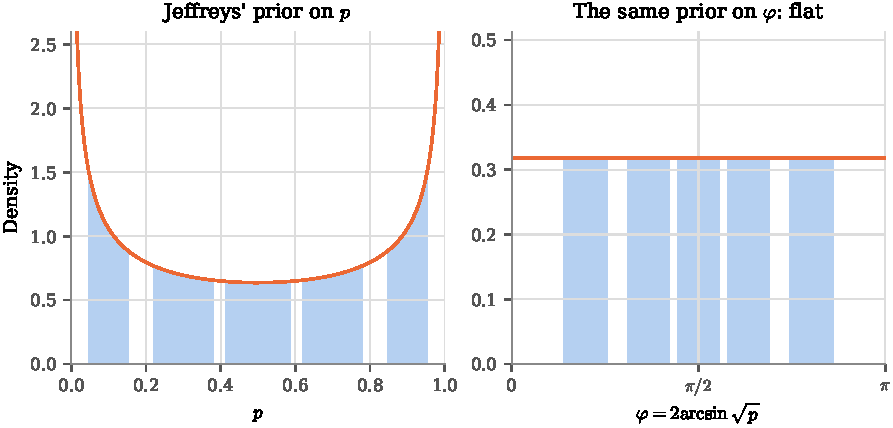
\includegraphics[width=\textwidth]{fig_jeffreys_equal_mass}
\caption{Jeffreys' prior for the kiss proportion (orange) with five bands $p_0 \pm 1.96\sqrt{p_0(1-p_0)/124}$, for $p_0 = 0.1, 0.3, 0.5, 0.7, 0.9$ (blue). Left: on $p$. Right: on $\varphi = 2\arcsin\sqrt{p}$, where the prior is flat.}
\label{fig:jeffequalmass}
\end{figure}

On the right of \cref{fig:jeffequalmass} the same bands are drawn on the scale $\varphi = 2\arcsin\sqrt{p}$, where they all have nearly the same width and the prior is flat.
That is not a coincidence: every one-parameter model has a scale on which its Jeffreys prior is flat.

\begin{proposition}[Jeffreys' prior is flat where the information is constant]
\label{prop:jeffreys-stabilizing}
In a one-parameter model satisfying the regularity conditions of \cref{sec:mle-regularity}, with $\Theta$ an interval and $I(\theta)$ continuous and positive on it, let $\varphi(\theta) = \int_{\theta_0}^\theta \sqrt{I(t)}\,\mathrm{d}t$ for a fixed $\theta_0 \in \Theta$. Then $I_\varphi \equiv 1$, Jeffreys' prior is flat in $\varphi$, and the maximum likelihood estimator satisfies $\sqrt{n}\big(\varphi(\hat{\theta}_n) - \varphi(\theta)\big) \convd \Gauss(0, 1)$ under $\Pr_\theta$ for every $\theta$ in the interior of $\Theta$: $\varphi$ is a variance-stabilizing transformation.
\end{proposition}

\recall{The delta method (\cref{thm:delta}): if $\sqrt{n}(Z_n - \theta) \convd \Gauss(0, \tau^2)$ and $g$ is continuously differentiable at $\theta$, then $\sqrt{n}\big(g(Z_n) - g(\theta)\big) \convd \Gauss\big(0, g'(\theta)^2\tau^2\big)$.}

\optionalproof{\Cref{lem:fisher-reparam} with $\mathrm{d}\varphi/\mathrm{d}\theta = \sqrt{I(\theta)}$, then the delta method.}
\begin{proof}
By the fundamental theorem of calculus, $\mathrm{d}\varphi/\mathrm{d}\theta = \sqrt{I(\theta)} > 0$, so $\varphi$ is strictly increasing, and \cref{lem:fisher-reparam} gives $I_\varphi = I_\theta(\mathrm{d}\theta/\mathrm{d}\varphi)^2 = I_\theta/I_\theta = 1$. Jeffreys' prior in $\varphi$ is then proportional to $\sqrt{1}$, a constant. By \cref{thm:mle-normal}, $\sqrt{n}(\hat{\theta}_n - \theta) \convd \Gauss(0, 1/I(\theta))$, and the delta method with $g = \varphi$, whose derivative $\sqrt{I}$ is continuous, gives the asymptotic variance $I(\theta) \cdot 1/I(\theta) = 1$.
\end{proof}

For the Bernoulli, $\int \mathrm{d}p/\sqrt{p(1-p)} = 2\arcsin\sqrt{p}$, which is why $\Betad(\frac12, \frac12)$ is also called the arcsine distribution.
For the Poisson, $I(\lambda) = 1/\lambda$ and $\varphi = 2\sqrt{\lambda}$.
For the exponential rate, $I(\lambda) = 1/\lambda^2$ and $\varphi = \log\lambda$: Jeffreys' prior $1/\lambda$ is flat in $\log\lambda$, and since $\log\beta = -\log\lambda$ it is flat in the log of the mean wait too.
So for the subway, where the flat prior on the rate and the flat prior on the wait disagreed (\cref{sec:jeff-flat}), Jeffreys' rule gives one answer: the prior $1/\lambda$ for the rate is the prior $1/\beta$ for the wait, and the posterior is $\Gammad(64, 398.7)$, between the two flat answers, with posterior mean $64/398.7 = 0.1605$, the maximum likelihood estimate.

\begin{bridge}[the arcsine and square-root transformations]
Applied courses in experimental design traditionally transform proportions by $\arcsin\sqrt{\hat{p}}$ and counts by $\sqrt{x}$ before comparing groups, so that every group has about the same variance whatever its mean.
These are the transformations of \cref{prop:jeffreys-stabilizing} for the Bernoulli and Poisson models, up to the factor $2$.
On those scales the Fisher information is constant, the standard error of the transformed estimate is $1/\sqrt{n}$ whatever the parameter, and Jeffreys' prior is flat.
For the kiss data, $2\arcsin\sqrt{0.645} = 1.865$ with standard error $1/\sqrt{124} = 0.090$, and the interval $1.865 \pm 1.96 \times 0.090$, mapped back to $p$, is $[0.559, 0.727]$, close to the Jeffreys posterior interval $[0.558, 0.725]$.
\end{bridge}

The table collects Jeffreys' prior for the book's one-parameter families, with the posterior after $n$ observations whose sum is $S$.
Only the first prior is proper, and each posterior is proper: for the Bernoulli always, for the Poisson, the exponential and the Gaussian mean once $n \geq 1$, and for the Gaussian scale once $n \geq 1$ and not every $x_i$ equals $\mu$.

\begin{center}
\small
\begin{tabular}{@{}llll@{}}
\toprule
model & $I$ & Jeffreys' prior & posterior \\
\midrule
$\Bern(p)$ & $1/(p(1-p))$ & $\Betad(\frac12, \frac12)$ & $\Betad(S + \frac12, n - S + \frac12)$ \\[2pt]
$\Pois(\lambda)$ & $1/\lambda$ & $\lambda^{-1/2}$, improper & $\Gammad(S + \frac12, n)$ \\[2pt]
$\Expo(\lambda)$ & $1/\lambda^2$ & $1/\lambda$, improper & $\Gammad(n, S)$ \\[2pt]
$\Gauss(\mu, \sigma^2)$, $\sigma$ known & $1/\sigma^2$ & $1$, improper & $\Gauss(\bar{x}, \sigma^2/n)$ \\[2pt]
$\Gauss(\mu, \sigma^2)$, $\mu$ known, in $\sigma$ & $2/\sigma^2$ & $1/\sigma$, improper & $\sum_i(x_i - \mu)^2/\sigma^2 \sim \chi^2_n$ \\
\bottomrule
\end{tabular}
\end{center}

\section{Several parameters: a Gaussian with unknown variance}
\label{sec:jeff-several}

\Cref{ch:bayes-intro} needed a prior for the wind turbine's $\sigma$ when it was unknown, used a density proportional to $1/\sigma$, independent of $\mu$, and promised this chapter would explain it.
The last row of the table is the explanation: $1/\sigma$ is Jeffreys' prior for $\sigma$ when $\mu$ is known, flat in $\log\sigma$.
With both parameters unknown, \cref{def:jeffreys} asks for the information matrix.
\Cref{sec:mle-fisher-examples} computed it for $(\mu, \sigma^2)$, and the matrix rule $I_\varphi = J^\top I_\theta J$ from the proof of \cref{thm:jeffreys-invariant}, with $J$ diagonal and $\mathrm{d}\sigma^2/\mathrm{d}\sigma = 2\sigma$, turns its entry $1/(2\sigma^4)$ into $(2\sigma)^2/(2\sigma^4) = 2/\sigma^2$:
\[
I(\mu, \sigma) = \begin{pmatrix} 1/\sigma^2 & 0 \\ 0 & 2/\sigma^2 \end{pmatrix}, \qquad \sqrt{\det I(\mu, \sigma)} = \frac{\sqrt{2}}{\sigma^2}.
\]
So Jeffreys' rule applied to $(\mu, \sigma)$ together gives the prior $1/\sigma^2$, not $1/\sigma$.
Jeffreys himself noticed the difference and recommended treating a location and a scale separately, each with its own one-parameter rule: flat in $\mu$, times $1/\sigma$.
The next result shows what the extra factor of $1/\sigma$ does.

\begin{proposition}[The posterior of a Gaussian mean with unknown variance]
\label{prop:jeff-t-posterior}
Given $(\mu, \sigma)$, let $\Xton$ be i.i.d.\ $\Gauss(\mu, \sigma^2)$, with $n \geq 2$, and let $\bar{x}$ and $s > 0$ be the observed sample mean and sample standard deviation. Take the improper prior $\pi(\mu, \sigma) = \sigma^{-k}$ on $\real \times (0, \infty)$, with $k = 1$ or $k = 2$. Then the posterior is proper, and the posterior distribution of $\mu$, with $\bar{x}$ and $s$ fixed, is given by
\[
\frac{\mu - \bar{x}}{s/\sqrt{n}} \sim t_{n-1} \quad (k = 1), \qquad \frac{\mu - \bar{x}}{s\sqrt{(n-1)/n}\big/\sqrt{n}} \sim t_n \quad (k = 2).
\]
\end{proposition}

\coreproof{Write the likelihood with $\sum_i(x_i - \mu)^2 = (n-1)s^2 + n(\bar{x} - \mu)^2$, integrate $\sigma$ out with a Gamma integral, and recognize Student's $t$ density in what is left.}
\begin{proof}
Adding and subtracting $\bar{x}$ inside the square, the cross term vanishes, and $A(\mu) = \sum_i(x_i - \mu)^2 = (n-1)s^2 + n(\bar{x} - \mu)^2$. The likelihood is $(2\pi)^{-n/2}\sigma^{-n}\exp(-A(\mu)/(2\sigma^2))$, so the posterior is proportional to $\sigma^{-(n+k)}\exp(-A(\mu)/(2\sigma^2))$. For fixed $\mu$, substitute $u = A(\mu)/(2\sigma^2)$, so that $\sigma = (A(\mu)/(2u))^{1/2}$ and $\mathrm{d}\sigma = -\frac12(A(\mu)/2)^{1/2}u^{-3/2}\,\mathrm{d}u$:
\begin{align*}
\int_0^\infty \sigma^{-(n+k)}e^{-A(\mu)/(2\sigma^2)}\,\mathrm{d}\sigma &= \frac12\Big(\frac{A(\mu)}{2}\Big)^{-(n+k-1)/2}\int_0^\infty u^{(n+k-3)/2}e^{-u}\,\mathrm{d}u \\
&= \frac12\Big(\frac{A(\mu)}{2}\Big)^{-(n+k-1)/2}\Gamma\Big(\frac{n+k-1}{2}\Big),
\end{align*}
finite since $n + k - 1 \geq 2$. So the posterior density of $\mu$ is proportional to $A(\mu)^{-(n+k-1)/2}$ and, after dividing $A(\mu)$ by the constant $(n-1)s^2$, to
\[
\Big(1 + \frac{t^2}{n-1}\Big)^{-(n+k-1)/2}, \qquad t = \frac{\mu - \bar{x}}{s/\sqrt{n}}.
\]
For $k = 1$ the exponent is $-((n-1) + 1)/2$, and this is the $t_{n-1}$ density of \cref{prop:student-props} in the variable $t$, without its constant. For $k = 2$ the exponent is $-(n+1)/2$; with $t' = t\sqrt{n/(n-1)}$ the ratio $t^2/(n-1)$ becomes $t'^2/n$, and this is the $t_n$ density in $t'$. Both are integrable in $\mu$, so the posterior is proper.
\end{proof}

For the wind turbine, $n = 12$, $\bar{x} = 14.3$ and $s = 4.7$.
With the prior $1/\sigma$ the posterior of $\mu$ is $14.3 + (4.7/\sqrt{12})\,t_{11}$.
Its middle $95\%$ is $14.3 \pm 2.20 \times 1.357 = [11.3, 17.3]$, the $t$-interval of \cref{ch:t-test} to the digit, and $\Pr(\mu > 10 \mid \text{data}) = \Pr(t_{11} > -3.17) = 0.9955$, which is one minus the $t$-test's one-sided $p$-value, $0.0045$.
With the prior $1/\sigma^2$ the posterior is narrower, $[11.5, 17.1]$, with $\Pr(\mu > 10 \mid \text{data}) = 0.9969$.
Read as a frequentist procedure, that narrower interval covers the true $\mu$ only $93.9\%$ of the time at $n = 12$ (\cref{ex:jeff-joint}), since it pairs $t_n$ quantiles with a scale that has $t_{n-1}$ behind it.
The product of the one-parameter rules reproduces the $t$ pivot exactly, the joint rule does not, and that is the usual reason for preferring $1/\sigma$; it is also the prior \cref{ch:bayes-intro} used.
The same Gamma integral shows why the posterior there was proper, although that chapter kept the prior $\Gauss(11, 2^2)$ for $\mu$: integrating $\sigma$ out leaves that Gaussian density times $A(\mu)^{-n/2}$, which is at most $((n-1)s^2)^{-n/2}$ since $A(\mu) \geq (n-1)s^2 > 0$, so the product is integrable; the $0.991$ found there is $\Pr(\mu > 10)$ under that posterior.

\Cref{fig:jefftreadings} draws the coincidence.
On the left, before the data and supposing $\mu = 10$, the standardized mean $\sqrt{12}(\bar{X}_{12} - 10)/S$ has the $t_{11}$ distribution, and the area beyond the observed $3.17$ is the $p$-value $0.0045$.
On the right, after the data, the posterior of $\mu$ is the same $t_{11}$ shape, centered at $14.3$ and scaled by $1.357$, and the area below $10$ is the same $0.0045$, now a probability for $\mu$.
The blue area is the $95\%$ $t$-interval, which here is also a region with posterior probability $0.95$.
One distribution answers both questions because the quantity $\sqrt{n}(\bar{x} - \mu)/s$ has the $t_{n-1}$ distribution in both readings: over repeated samples with $\mu$ fixed, and over $\mu$ with the sample fixed.

\begin{figure}[htbp]
\centering
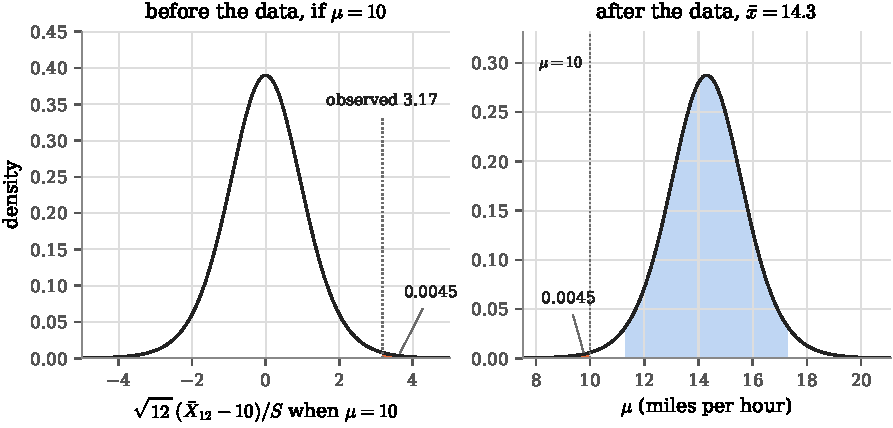
\includegraphics[width=\textwidth]{fig_jeffreys_t_two_readings}
\caption{One $t_{11}$ density read two ways, for the wind turbine. Left: the standardized mean when $\mu = 10$; orange, the area above the observed $3.17$. Right: the posterior of $\mu$ under the prior $1/\sigma$; orange, the area below $10$; blue, the $95\%$ $t$-interval.}
\label{fig:jefftreadings}
\end{figure}

\begin{bridge}[the $t$-interval is also a Bayesian interval]
An introductory course computes $\bar{x} \pm t^*s/\sqrt{n}$ and warns that `there is a $95\%$ probability that $\mu$ is in the interval' is the wrong sentence, since $\mu$ is fixed and the interval is random.
Under the prior flat in $\mu$ times $1/\sigma$, \cref{prop:jeff-t-posterior} makes that sentence true, with the same numbers: the probability is a posterior probability, conditional on the data, and it holds under this prior, not under every prior.
The $z$-interval with $\sigma$ known has the same double reading under the flat prior on $\mu$, whose posterior is $\Gauss(\bar{x}, \sigma^2/n)$.
\end{bridge}

\section{Bayesian confidence regions}
\label{sec:jeff-regions}

A posterior answers `where is $\theta$?' with a whole distribution.
A region that holds most of that distribution is the Bayesian counterpart of a confidence interval, and there is more than one way to choose it.

\begin{definition}[Bayesian confidence region]
\label{def:bayes-region}
Let $\alpha \in (0, 1)$, and let the posterior have a density. A \textbf{Bayesian confidence region of level $1 - \alpha$} is a set $R(\mathbf{x}) \subseteq \Theta$, computed from the data, with posterior probability $\Pr(\theta \in R(\mathbf{x}) \mid \mathbf{x}) = 1 - \alpha$. For a real parameter, the \textbf{equal-tailed} region is the interval from the point with posterior probability $\alpha/2$ below it to the point with posterior probability $\alpha/2$ above it. The \textbf{highest posterior density} region is $\{\theta : \pi(\theta \mid \mathbf{x}) \geq c\}$, with $c$ chosen so that its posterior probability is $1 - \alpha$.
\end{definition}

\begin{inwords}
\textbf{In words.} A region that holds $95\%$ of the posterior. The equal-tailed one cuts $2.5\%$ off each end; the highest-density one keeps the most probable values, those where the posterior density is above some height. Most texts call these credible regions, or credible intervals. This book calls $1 - \alpha$ the level, as for the confidence intervals of \cref{ch:confidence-intervals}, although some texts call $\alpha$ the level of a Bayesian region.
\par\smallskip
\textbf{For the kiss data.} Under Jeffreys' prior the posterior is $\Betad(80.5, 44.5)$. Its equal-tailed $95\%$ region is $[0.558, 0.725]$ and its highest-density region is $[0.560, 0.727]$, slightly to the right, toward the posterior's mode $0.646$: the posterior has a longer tail to the left.
\end{inwords}

The two kinds of region promise different things.
The highest-density region is the shortest region with the stated probability; the equal-tailed region follows the parameter through any monotone change of scale.

\begin{proposition}[The highest-density region is the shortest]
\label{prop:hpd-shortest}
Let the posterior have a density $f$ on $\real$, and let $H = \{\theta : f(\theta) \geq c\}$, with $c > 0$, have posterior probability $1 - \alpha$. Every set $R$ with posterior probability at least $1 - \alpha$ is at least as long as $H$.
\end{proposition}

\optionalproof{Compare the parts where $R$ and $H$ differ: the part only in $H$ has density at least $c$ and the part only in $R$ at most $c$, so $R$ needs at least as much length to hold at least as much probability.}
\begin{proof}
Write $\abs{A}$ for the length of a set $A$ and $P(A)$ for its posterior probability. Since $P(R) \geq P(H)$ and the two share $R \cap H$, $P(R \setminus H) \geq P(H \setminus R)$. On $R \setminus H$ the density is below $c$, so $P(R \setminus H) \leq c\abs{R \setminus H}$; on $H \setminus R$ it is at least $c$, so $P(H \setminus R) \geq c\abs{H \setminus R}$. Hence $c\abs{R \setminus H} \geq c\abs{H \setminus R}$, and dividing by $c$ and adding $\abs{R \cap H}$ to both sides gives $\abs{R} \geq \abs{H}$.
\end{proof}

The equal-tailed region has the other property.
If $\varphi = g(\theta)$ with $g$ increasing, the point with posterior probability $\alpha/2$ below it for $\varphi$ is $g$ of the corresponding point for $\theta$, so the equal-tailed region for $\varphi$ is the image of the one for $\theta$.
The highest-density region has no such guarantee, since the posterior density of $\varphi$ carries the factor $\abs{\mathrm{d}\theta/\mathrm{d}\varphi}$ of \cref{eq:jeff-change}, which changes which values count as most probable.

The wind turbine's $\sigma$ shows the difference.
Under the prior flat in $\mu$ times $1/\sigma$, integrating $\mu$ out of $\sigma^{-(n+1)}\exp(-A(\mu)/(2\sigma^2))$ leaves the posterior $\sigma^{-n}\exp(-(n-1)s^2/(2\sigma^2))$ for $\sigma$, since $A(\mu) = (n-1)s^2 + n(\mu - \bar{x})^2$ and the Gaussian integral $\int \exp(-n(\mu - \bar{x})^2/(2\sigma^2))\,\mathrm{d}\mu = \sigma\sqrt{2\pi/n}$ contributes one factor of $\sigma$.
The change of variables $v = (n-1)s^2/\sigma^2$, with $\sigma = s\sqrt{(n-1)/v}$ and $\abs{\mathrm{d}\sigma/\mathrm{d}v} \propto v^{-3/2}$, turns this into a density proportional to $v^{n/2}e^{-v/2}v^{-3/2} = v^{(n-1)/2 - 1}e^{-v/2}$, the $\chi^2_{n-1}$ density of \cref{prop:chisq-props}: $(n-1)s^2/\sigma^2$, with $\sigma$ random and $s$ fixed, has the $\chi^2_{n-1}$ distribution.
That is the distribution Cochran's theorem (\cref{thm:cochran}) gives $(n-1)S^2/\sigma^2$ over repeated samples, so here too the equal-tailed region coincides with the frequentist interval built from that pivot: $[3.33, 7.98]$ for $\sigma$ and, squared, $[11.1, 63.7]$ for $\sigma^2$.
The highest-density regions are $[3.08, 7.45]$ for $\sigma$ and $[8.5, 53.9]$ for $\sigma^2$, each shorter than the equal-tailed region on its own scale.
But the square of the first is $[9.5, 55.5]$, not the second: shortest on the scale of $\sigma$ and shortest on the scale of $\sigma^2$ are different requirements.
\Cref{fig:jeffhpd} shows both scales.

\begin{figure}[htbp]
\centering
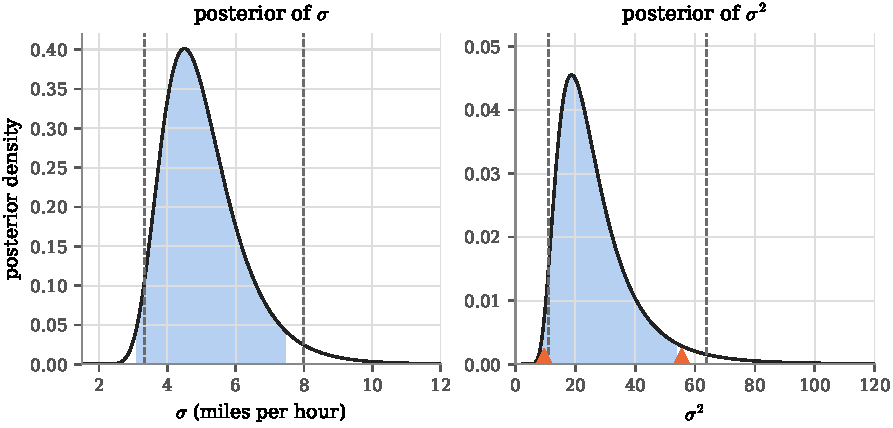
\includegraphics[width=\textwidth]{fig_jeffreys_hpd}
\caption{Posterior of the wind turbine's $\sigma$ (left) and $\sigma^2$ (right) under the prior $1/\sigma$. Blue: the $95\%$ highest-density regions. Gray dashed: the equal-tailed regions. Orange triangles: the squares of the endpoints of the left highest-density region.}
\label{fig:jeffhpd}
\end{figure}

\begin{pitfall}[the shortest region depends on the scale]
`The $95\%$ highest-density interval' is not a property of the posterior alone: it also depends on whether length is measured in $\sigma$ or in $\sigma^2$, in $p$ or in $\psi$.
When the parameterization is a matter of convention, report the equal-tailed region, which follows the parameter through every monotone change of scale, or say on which scale the highest-density region was computed.
\end{pitfall}

The subway shows the same exact coincidence for a rate.
Under Jeffreys' prior its posterior is $\Gammad(64, 398.7)$, whose $2.5\%$ and $97.5\%$ points are $49.29/398.7 = 0.124$ and $80.60/398.7 = 0.202$, where $49.29$ and $80.60$ are the corresponding points of $\Gammad(64, 1)$.
That is exactly the interval of \cref{ex:ci-gamma}, built from the pivot $\lambda\sum_i T_i \sim \Gammad(64, 1)$.
Again one distribution is read twice: over repeated samples with $\lambda$ fixed, $\lambda\sum_i T_i$ is $\Gammad(64, 1)$; over $\lambda$ with the sample fixed, the posterior $\Gammad(64, 398.7)$ makes $398.7\lambda$ a $\Gammad(64, 1)$ variable.
The two sentences come apart only in what they are about.
`Of $1{,}000$ subway studies of $64$ waits each, the interval computed from each covers the true rate in about $950$' is a statement about the procedure.
`Given these $64$ waits and Jeffreys' prior, the rate lies in $[0.124, 0.202]$ with probability $0.95$' is a statement about $\lambda$: the first of the three readings that \cref{sec:ci-meaning} ruled out for a confidence interval, true here under a prior.

\begin{sanitycheck}[Should the posterior mean wait be $1/0.1605$?]
Under Jeffreys' prior the posterior mean of the rate is $64/398.7 = 0.1605$, the maximum likelihood estimate, so it is tempting to call $1/0.1605 = 6.23$ minutes the posterior mean of the wait.
It is not: the wait $\beta = 1/\lambda$ has posterior mean $\E[1/\lambda \mid \text{data}] = 398.7/63 = 6.33$ minutes, larger, as Jensen's inequality says it must be, since $1/\lambda$ is convex \toolkit{sec:math-convex}.
Means do not follow a nonlinear change of scale, but quantiles do: the posterior median of the rate is $0.1597$, and the posterior median of the wait is $1/0.1597 = 6.26$ minutes.
\end{sanitycheck}

\section{When the two kinds of interval agree}
\label{sec:jeff-agree}

The exact coincidences of the last two sections, the $z$- and $t$-intervals, the chi-squared interval for $\sigma$ and the subway's Gamma interval, all come from location and scale families with the matching improper prior, flat for a location and $1/\text{scale}$ for a scale: there the posterior distribution of the pivot equals its sampling distribution.
In other models the two kinds of interval agree only approximately, and the Bernstein--von Mises theorem says how.

\recall{The Bernstein--von Mises theorem (\cref{thm:bvm}): for i.i.d.\ data from a model satisfying the regularity conditions of \cref{sec:mle-regularity}, with $\theta^*$ in the interior of $\Theta$, $I(\theta^*) > 0$, data that separate $\theta^*$ from distant values, and a prior density continuous and positive at $\theta^*$, the posterior distribution of $\sqrt{n}(\theta - \hat{\theta}_n)$ approaches $\Gauss(0, 1/I(\theta^*))$ in total variation, in probability. Slutsky's theorem (\cref{thm:slutsky}): if $X_n \convd X$ and $Y_n \convp c$ for a constant $c$, then $X_n + Y_n \convd X + c$.}

Closeness in total variation makes every posterior probability, and so every posterior quantile of $\sqrt{n}(\theta - \hat{\theta}_n)$, close to the Gaussian one.
So the equal-tailed region of level $1 - \alpha$ is $\hat{\theta}_n \pm q_{\alpha/2}/\sqrt{nI(\theta^*)}$ up to an error that is negligible next to $1/\sqrt{n}$.
It covers $\theta^*$ exactly when $\sqrt{n}(\hat{\theta}_n - \theta^*)$ lies between $-q_{\alpha/2}/\sqrt{I(\theta^*)}$ and $q_{\alpha/2}/\sqrt{I(\theta^*)}$, each moved by a term that converges to $0$ in probability, so by \cref{thm:mle-normal} and Slutsky's theorem, applied at each end, the Bayesian region has asymptotic coverage $1 - \alpha$, the same as the plug-in interval $\hat{\theta}_n \pm q_{\alpha/2}/\sqrt{nI(\hat{\theta}_n)}$ of \cref{ch:mle-properties}, whatever the prior, as long as its density is continuous and positive at $\theta^*$.
With an improper prior the same can be checked in each example of this chapter, whose posteriors are explicit.
For the kiss data the priors of this chapter give $95\%$ regions within $0.003$ of each other and of the solve interval of \cref{ch:confidence-intervals}, $[0.558, 0.724]$: flat $[0.558, 0.724]$, Jeffreys $[0.558, 0.725]$, Haldane $[0.559, 0.727]$.

How fast the agreement comes depends on the prior, and for one-sided bounds Jeffreys' prior is special.
For a one-parameter model with continuous data, Welch and Peers (\textit{Journal of the Royal Statistical Society B}, 1963) showed that the posterior's one-sided bounds have frequentist coverage $1 - \alpha$ up to an error of order $1/n$ when the prior is Jeffreys', and of order only $1/\sqrt{n}$ for other smooth priors.
In an equal-tailed region the two errors of order $1/\sqrt{n}$ cancel, so its coverage error is of order $1/n$ under any smooth prior.
These results are stated without proof; their proof needs more than this book develops, and nothing later depends on them.
For a proportion no interval has coverage exactly $1 - \alpha$ at every $p$, since the data are discrete, but the Jeffreys interval, the equal-tailed region of $\Betad(S + \frac12, n - S + \frac12)$, comes close.
At $p = 0.645$ and $n = 124$ its coverage is $0.952$, the same as the solve interval's, where the plug-in interval has $0.939$.
At $n = 20$, averaged over $p$ from $0.01$ to $0.99$, the coverage is $0.951$ for the Jeffreys interval, $0.954$ for the solve interval and $0.861$ for the plug-in interval.
\Cref{fig:jeffcoverage} draws the solve and Jeffreys intervals at $n = 20$: both oscillate around $0.95$, the solve interval dropping lowest at the very ends ($0.84$ just below $p = 0.009$) and the Jeffreys interval at $p = 0.12$ and $0.88$ ($0.89$).
Of $1{,}000$ studies of $20$ couples, the Jeffreys interval covers the true $p$ in about $951$ on average over $p$, the plug-in interval in about $861$.
Brown, Cai and DasGupta (\textit{Statistical Science}, 2001) recommend the solve (Wilson) interval or the Jeffreys interval for small $n$, the latter modified when $S$ is $0$, $1$, $n - 1$ or $n$: as defined here, the interval for $S = 0$ starts above $0$ (at $0.000024$ when $n = 20$), so its coverage is $0$ for $p$ closer to $0$ than that.

\begin{figure}[htbp]
\centering
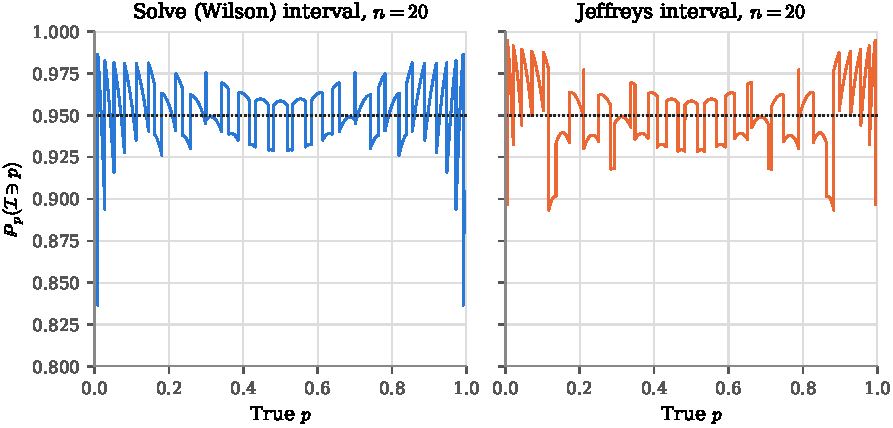
\includegraphics[width=\textwidth]{fig_jeffreys_coverage}
\caption{Exact coverage $\Pr_p(\mathcal{I} \ni p)$ of two $95\%$ intervals for a proportion at $n = 20$, against the true $p$: left, the solve (Wilson) interval (blue); right, the equal-tailed Jeffreys interval (orange). Dotted: the nominal $0.95$.}
\label{fig:jeffcoverage}
\end{figure}

The agreement has limits, and \cref{ch:bayes-intro} has already shown two.
With an informative prior and moderate $n$ the regions differ: the skeptic's prior gave the interval $[0.56, 0.73]$ posterior probability $0.835$, not $0.95$.
For a point null the answers differ at every $n$: a prior with a lump of probability at $p = \frac12$ has no density, so the Bernstein--von Mises theorem does not apply, and $\Pr(H_0 \mid \mathbf{x}) = 0.044$ stood against a $p$-value of $0.0012$.

\section{What comes next}
\label{sec:jeff-next}

This chapter ends Part VII.
Part VIII returns to the frequentist methods of the earlier parts and applies them to a model with a predictor, the linear regression model of \cref{ch:regression-uni}, where least squares, the method that led Gauss to the distribution named after him (\cref{ch:gaussian}), is the estimator.
The Bayesian reading carries over: with Gaussian errors, the least squares estimate is the posterior mode under a flat prior on the coefficients, and with a Gaussian prior centered at zero the posterior mode is the ridge estimate that \cref{ch:bayes-intro} mentioned.

\section{Summary}
\label{sec:jeff-summary}

\begin{itemize}[nosep]
\item A flat prior is flat on one scale only. By the change of variables formula $\pi_\varphi = \pi_\theta\abs{\mathrm{d}\theta/\mathrm{d}\varphi}$, flat in $p$ is the logistic density in the log-odds, and flat in the subway's mean wait is $1/\lambda^2$ in terms of the rate; at $n = 64$ the two flat answers for the subway differ by a quarter of a posterior standard deviation.
\item An improper prior has an infinite integral. It gives a posterior when $0 < \int L_n\pi < \infty$, and none otherwise (Haldane's prior when every couple turns right). It can be read as the limit of wider and wider proper priors, and its arbitrary constant cancels in estimation but makes the Bayes factor arbitrary when it is the prior for the parameter that a point null fixes.
\item Fisher information changes with the parameterization as $I_\varphi = I_\theta(\mathrm{d}\theta/\mathrm{d}\varphi)^2$, so Jeffreys' prior $\pi_J \propto \sqrt{I}$, or $\sqrt{\det I}$ in several dimensions, is the same prior whichever parameterization it is computed in. It gives equal mass to intervals the data can just tell apart, and it is flat on the variance-stabilizing scale $\int\sqrt{I}$: $2\arcsin\sqrt{p}$, $2\sqrt{\lambda}$, $\log\lambda$.
\item Jeffreys' priors: $\Betad(\frac12, \frac12)$ for a proportion (kiss posterior mean $0.644$), $\lambda^{-1/2}$ for a Poisson mean, $1/\lambda$ for a rate (subway posterior mean $0.1605$, the maximum likelihood estimate), flat for a Gaussian mean, $1/\sigma$ for a scale. For a Gaussian with both parameters unknown the joint rule gives $1/\sigma^2$, and the product of the separate rules, $1/\sigma$, is the one that reproduces the $t$-interval.
\item A Bayesian confidence region of level $1 - \alpha$ has posterior probability $1 - \alpha$. The highest-density region is the shortest; the equal-tailed region follows the parameter through any monotone change of scale, and the highest-density region does not.
\item With the matching improper prior, Bayesian regions equal frequentist intervals exactly in location and scale families: the $z$- and $t$-intervals, the chi-squared interval for $\sigma$, the subway's exact $[0.124, 0.202]$. Elsewhere they agree as $n$ grows (Bernstein--von Mises); for one-sided bounds the agreement is fastest under Jeffreys' prior (Welch and Peers), and the Jeffreys interval for a proportion covers about $95\%$ of the time on average over $p$ even at $n = 20$.
\end{itemize}

\section{Exercises}
\label{sec:jeff-exercises}

\begin{exercise}
\label{ex:jeff-poisson}
(a) Show that Jeffreys' prior for the Poisson mean is $\lambda^{-1/2}$, that it is improper, and that after $n \geq 1$ observations with sum $S$ the posterior is $\Gammad(S + \frac12, n)$. (b) The siblings data of \cref{ch:models} have $24$ values of $X - 1$ adding up to $24$. Find the posterior mean of $\lambda$ under Jeffreys' prior and under the flat prior $\pi(\lambda) = 1$, and compare with the maximum likelihood estimate.
\end{exercise}
\begin{solution}
(a) $I(\lambda) = 1/\lambda$ (\cref{sec:mle-fisher-examples}), so $\pi_J(\lambda) \propto \lambda^{-1/2}$, and $\int_0^M \lambda^{-1/2}\,\mathrm{d}\lambda = 2\sqrt{M} \to \infty$: improper. The likelihood is proportional to $\lambda^{S}e^{-n\lambda}$, so the posterior is proportional to $\lambda^{S - 1/2}e^{-n\lambda}$, the $\Gammad(S + \frac12, n)$ density, whose integral is finite for every $S \geq 0$ once $n \geq 1$. (b) Jeffreys: $\Gammad(24.5, 24)$, mean $24.5/24 = 1.021$. Flat: $\Gammad(25, 24)$, mean $25/24 = 1.042$. The maximum likelihood estimate is $24/24 = 1$. Jeffreys' prior adds half a count to $S$ and the flat prior a whole count.
\end{solution}

\begin{exercise}
\label{ex:jeff-geometric}
A geometric observation counts the trials up to and including the first success, $\Pr_p(X = x) = p(1-p)^{x-1}$ for $x = 1, 2, \ldots$, with $\E_p[X] = 1/p$. (a) Show that $I(p) = 1/(p^2(1-p))$, so Jeffreys' prior is $p^{-1}(1-p)^{-1/2}$, and that it is improper. (b) Suppose an observer watched kissing couples until the first right turn, five times over, needing $1$, $2$, $1$, $1$ and $3$ couples. Show that Jeffreys' posterior is $\Betad(5, 3.5)$ and find its mean. (c) The same eight couples, read as eight Bernoulli trials with five right turns, have a likelihood proportional to the same function of $p$. What is Jeffreys' posterior mean for them, and what does the difference say about Jeffreys' prior?
\end{exercise}
\begin{solution}
(a) $\ell(p) = \log p + (X - 1)\log(1-p)$, so $\ell''(p) = -1/p^2 - (X - 1)/(1-p)^2$, and with $\E_p[X - 1] = (1-p)/p$, $I(p) = 1/p^2 + 1/(p(1-p)) = (1 - p + p)/(p^2(1-p)) = 1/(p^2(1-p))$. So $\pi_J(p) \propto p^{-1}(1-p)^{-1/2}$, whose integral diverges at $p = 0$ like $\int \mathrm{d}p/p$. (b) The likelihood of $n = 5$ observations with sum $8$ is $p^5(1-p)^{8-5}$, and times the prior it is $p^4(1-p)^{2.5}$: the $\Betad(5, 3.5)$ density, with mean $5/8.5 = 0.588$. (c) Jeffreys' prior for Bernoulli trials is $\Betad(\frac12, \frac12)$, and the posterior is $\Betad(5.5, 3.5)$, with mean $5.5/9 = 0.611$. The likelihoods are the same, but the priors differ because the Fisher information depends on how the data were collected, not only on the likelihood they produced: Jeffreys' prior depends on the sampling plan.
\end{solution}

\begin{exercise}
\label{ex:jeff-scale}
Let $\Xton \iid \Gauss(\mu, v)$ with $\mu$ known, parameterized by the variance $v = \sigma^2$. (a) Show that Jeffreys' prior for $v$ is proportional to $1/v$. (b) Show that carrying the prior $1/\sigma$ on $\sigma$ to $v$ by \cref{eq:jeff-change} gives $1/v$ up to a constant, as \cref{thm:jeffreys-invariant} says it must. (c) Show that the prior $1/\sigma$ is the flat prior on $\log\sigma$, and that rescaling, $\sigma' = c\sigma$ for a constant $c > 0$, such as a change from miles to kilometers per hour, leaves it in the same form.
\end{exercise}
\begin{solution}
(a) By \cref{sec:mle-fisher-examples}, the information for the variance is $1/(2v^2)$, and its square root is $1/(\sqrt{2}\,v) \propto 1/v$. (b) $\sigma = \sqrt{v}$ and $\mathrm{d}\sigma/\mathrm{d}v = 1/(2\sqrt{v})$, so the prior on $v$ is $\frac{1}{\sqrt{v}} \cdot \frac{1}{2\sqrt{v}} = \frac{1}{2v} \propto \frac1v$. (c) With $\eta = \log\sigma$, $\mathrm{d}\eta/\mathrm{d}\sigma = 1/\sigma$, so a constant density in $\eta$ is $1/\sigma$ in $\sigma$ by \cref{eq:jeff-change}. Under $\sigma' = c\sigma$, $\mathrm{d}\sigma/\mathrm{d}\sigma' = 1/c$ and $\pi(\sigma') = \frac{1}{\sigma'/c} \cdot \frac1c = \frac{1}{\sigma'}$, the same form.
\end{solution}

\begin{exercise}
\label{ex:jeff-haldane}
(a) Show that under Haldane's prior $\pi(p) = 1/(p(1-p))$ the posterior after $S$ successes in $n$ trials is $\Betad(S, n - S)$ when $0 < S < n$, and that its mean is the sample proportion. (b) Show that there is no posterior when $S = 0$, and that under Jeffreys' prior there is one for every $S$. (c) Give the posterior means of $p$ for the kiss data under the flat, Jeffreys and Haldane priors, and say which way each prior pulls the estimate.
\end{exercise}
\begin{solution}
(a) $L_n\pi = p^S(1-p)^{n-S}/(p(1-p)) = p^{S-1}(1-p)^{n-S-1}$, integrable when $S \geq 1$ and $n - S \geq 1$; it is the $\Betad(S, n - S)$ density, with mean $S/n$. (b) With $S = 0$, $L_n\pi = p^{-1}(1-p)^{n-1}$, whose integral diverges at $p = 0$ like $\int \mathrm{d}p/p$, so $m(\mathbf{x}) = \infty$. Under Jeffreys' prior the posterior is $\Betad(S + \frac12, n - S + \frac12)$, both of whose parameters are at least $\frac12$ for every $S$. (c) Flat: $81/126 = 0.643$; Jeffreys: $80.5/125 = 0.644$; Haldane: $80/124 = 0.645$. The flat prior adds one imaginary success and one failure and pulls toward $\frac12$ the most, Jeffreys' prior adds half of each, and Haldane's adds none.
\end{solution}

\begin{exercise}
\label{ex:jeff-subway-wait}
For the subway, under each of the three priors of this chapter for the rate (flat in $\lambda$, Jeffreys' $1/\lambda$, flat in the wait $\beta$), the posterior of $\lambda$ is $\Gammad(a, 398.7)$ with $a = 65$, $64$ and $63$. (a) Show that the posterior mean of the wait $\beta = 1/\lambda$ is $398.7/(a - 1)$, and compute it for the three priors. (b) The $95\%$ equal-tailed regions for $\lambda$ are $[0.1258, 0.2050]$, $[0.1236, 0.2022]$ and $[0.1214, 0.1994]$. Give the equal-tailed regions for $\beta$ without further computation. (c) Which prior makes the posterior mean of $\beta$ equal to the maximum likelihood estimate $6.23$, and which makes the posterior mean of $\lambda$ equal to $1/6.23$?
\end{exercise}
\begin{solution}
(a) $\E[1/\lambda] = \int_0^\infty \frac1\lambda\,\frac{b^a}{\Gamma(a)}\lambda^{a-1}e^{-b\lambda}\,\mathrm{d}\lambda = \frac{b^a}{\Gamma(a)}\cdot\frac{\Gamma(a-1)}{b^{a-1}} = \frac{b}{a-1}$, using $\Gamma(a) = (a-1)\Gamma(a-1)$. With $b = 398.7$: $6.23$, $6.33$ and $6.43$ minutes. (b) The map $\lambda \mapsto 1/\lambda$ is decreasing, so the equal-tailed region for $\beta$ is $[1/U, 1/L]$: $[4.88, 7.95]$, $[4.95, 8.09]$ and $[5.02, 8.24]$ minutes. (c) The flat prior on $\lambda$ ($a = 65$) gives posterior mean wait $398.7/64 = 6.23$; Jeffreys' prior ($a = 64$) gives posterior mean rate $64/398.7 = 0.1605 = 1/6.23$. No prior makes both means equal to the maximum likelihood estimates, since $\E[1/\lambda] > 1/\E[\lambda]$.
\end{solution}

\begin{exercise}
\label{ex:jeff-joint}
Under the prior $1/\sigma^2$ of \cref{prop:jeff-t-posterior}, the $95\%$ equal-tailed region for $\mu$ is $\bar{x} \pm q_{0.025}(t_n)\sqrt{(n-1)/n}\,s/\sqrt{n}$. (a) Show that, read as a confidence interval, its coverage is $\Pr(\abs{T} \leq q_{0.025}(t_n)\sqrt{(n-1)/n})$ with $T \sim t_{n-1}$, whatever $\mu$ and $\sigma$ are. (b) Evaluate it at $n = 5$, given $q_{0.025}(t_5) = 2.5706$ and $\Pr(\abs{t_4} \leq 2.299) = 0.917$. (c) What is the coverage of the region under the prior $1/\sigma$?
\end{exercise}
\begin{solution}
(a) The interval contains $\mu$ exactly when $\abs{\sqrt{n}(\bar{X}_n - \mu)/S} \leq q_{0.025}(t_n)\sqrt{(n-1)/n}$, and by \cref{thm:t-pivot} the left side is $\abs{T}$ with $T \sim t_{n-1}$ for every $\mu$ and $\sigma$. (b) $2.5706 \times \sqrt{4/5} = 2.299$, so the coverage is $0.917$, against the nominal $0.95$; at $n = 12$ it is $0.939$. (c) Exactly $0.95$: under $1/\sigma$ the region is $\bar{x} \pm q_{0.025}(t_{n-1})s/\sqrt{n}$, the $t$-interval.
\end{solution}

\begin{exercise}
\label{ex:jeff-bayes-factor}
Test $H_0: p = \frac12$ against $H_1: p \neq \frac12$ for the kiss data, with prior probability $\frac12$ on each, as in \cref{sec:bayes-hypotheses}, but with Haldane's prior $c/(p(1-p))$ on $H_1$. (a) Show that $m_1 = c\,B(80, 44)$, where $B(a, b) = \int_0^1 p^{a-1}(1-p)^{b-1}\,\mathrm{d}p$. (b) Given $B(80, 44) = 4.45 \times 10^{-36}$ and $m_0 = 2^{-124} = 4.70 \times 10^{-38}$, compute $B_{01}$ and $\Pr(H_0 \mid \mathbf{x})$ for $c = 1$ and for $c = 1{,}000$. (c) Why does the constant not matter when the same prior is used to estimate $p$?
\end{exercise}
\begin{solution}
(a) $m_1 = \int_0^1 p^{80}(1-p)^{44}\,\frac{c}{p(1-p)}\,\mathrm{d}p = c\int_0^1 p^{79}(1-p)^{43}\,\mathrm{d}p = c\,B(80, 44)$. (b) $c = 1$: $B_{01} = 4.70 \times 10^{-38}/(4.45 \times 10^{-36}) = 0.0106$ and $\Pr(H_0 \mid \mathbf{x}) = 0.0106/1.0106 = 0.0105$. $c = 1{,}000$: $B_{01} = 1.06 \times 10^{-5}$ and $\Pr(H_0 \mid \mathbf{x}) = 1.06 \times 10^{-5}$. Nothing in the data or the model picks $c$. (c) The posterior under $H_1$ is $c\,p^{79}(1-p)^{43}/(c\,B(80, 44))$, and $c$ cancels.
\end{solution}

\begin{exercise}
\label{ex:jeff-symmetric}
(a) Show that if a posterior density on $\real$ is symmetric about a point $m$ and decreases as $\abs{\theta - m}$ grows, its highest-density and equal-tailed regions of every level coincide. (b) Which posteriors of this chapter are of that kind, and which are not?
\end{exercise}
\begin{solution}
(a) The set where the density is at least $c$ is an interval $[m - h, m + h]$, symmetric about $m$, and by symmetry it leaves the same posterior probability $\alpha/2$ outside it on each side. So the highest-density region with probability $1 - \alpha$ is the equal-tailed one. (b) The posterior $\Gauss(\bar{x}, \sigma^2/n)$ of a Gaussian mean and the $t$ posteriors of \cref{prop:jeff-t-posterior} are of that kind. The Beta posteriors of the kiss data, the Gamma posteriors of the subway and the posteriors of $\sigma$ and $\sigma^2$ are skewed, and there the two regions differ.
\end{solution}

\begin{exercise}
\label{ex:jeff-location}
Let $X$ have density $f(x - \theta)$, with $f$ a known density on $\real$ (a location family), and take the improper prior $\pi(\theta) = 1$. (a) Show that the posterior density of $\theta$ given $X = x$ is $f(x - \theta)$. (b) Let $u(x)$ be the posterior's upper bound of level $1 - \alpha$: $\Pr(\theta \leq u(x) \mid x) = 1 - \alpha$. Show that $\Pr_\theta(\theta \leq u(X)) = 1 - \alpha$ for every $\theta$: the Bayesian bound has exact frequentist coverage.
\end{exercise}
\begin{solution}
(a) $L(x; \theta)\pi(\theta) = f(x - \theta)$, and $\int f(x - \theta)\,\mathrm{d}\theta = \int f(w)\,\mathrm{d}w = 1$, so $m(x) = 1$ and the posterior is $f(x - \theta)$. (b) Given $x$, $\theta = x - W$ with $W$ having density $f$, so $\theta \leq u(x)$ exactly when $W \geq x - u(x)$. The posterior condition says $\Pr(W \geq x - u(x)) = 1 - \alpha$, so $x - u(x) = w$, the point with probability $\alpha$ below it under $f$, the same for every $x$, and $u(x) = x - w$. Under $\Pr_\theta$, $X = \theta + W'$ with $W'$ having density $f$, and $\theta \leq X - w$ exactly when $W' \geq w$, which has probability $1 - \alpha$.
\end{solution}

\begin{exercise}
\label{ex:jeff-drug}
In the drug trial of \cref{ch:kiss}, $78$ of $100$ patients were cured. (a) Give Jeffreys' posterior, its mean and its $95\%$ equal-tailed region, given that the $2.5\%$ and $97.5\%$ points of the posterior are $0.692$ and $0.852$. (b) Compute the arcsine interval $2\arcsin\sqrt{\hat{p}} \pm 1.96/\sqrt{n}$, mapped back to $p$, and compare with (a), with the solve interval $[0.689, 0.850]$ of \cref{eq:wilson} and with the plug-in interval $[0.699, 0.861]$ of \cref{ch:kiss}.
\end{exercise}
\begin{solution}
(a) $\Betad(78.5, 22.5)$, with mean $78.5/101 = 0.777$ and $95\%$ region $[0.692, 0.852]$. (b) $2\arcsin\sqrt{0.78} = 2.165$ and $1.96/\sqrt{100} = 0.196$, so $\varphi \in [1.969, 2.361]$, and $p = \sin^2(\varphi/2)$ gives $[0.694, 0.855]$. The Jeffreys, arcsine and solve intervals agree to within about $0.005$ and all sit to the left of the plug-in interval, which is symmetric about $0.78$ although the binomial is skewed this close to $1$.
\end{solution}


\partintro{Least squares as a statistical model. One predictor first (\cref{ch:regression-uni}), then the matrix form with several, and the inference that comes with Gaussian errors (\cref{ch:regression-multi}), where the identifiability of \cref{ch:models} returns as the rank of the design matrix.}
\part{Linear Regression}
\chapter{Univariate Linear Regression}
\label{ch:regression-uni}

% Not yet written. Source material: notes ch. Univariate Linear Regression; unit 7 slides

\chapter{Multivariate Linear Regression and Inference}
\label{ch:regression-multi}

\begin{chaptergoals}
\begin{itemize}[nosep]
\item Several predictors at once: the model $Y = X\beta + \epsilon$ with a design matrix $X$, which also covers polynomials, $0/1$ variables and the previous eruption's wait and duration for Old Faithful.
\item Least squares in matrix form, $\hat{\beta} = (X^\top X)^{-1}X^\top Y$, and what it is: the projection of the response vector onto the space spanned by the columns of $X$. Full rank as identifiability.
\item With Gaussian errors: the distribution of $\hat{\beta}$, the residual variance on $n - p$ degrees of freedom by the general form of Cochran's theorem, the exact $t$-test for one coefficient and the $F$-test for several, which is the likelihood ratio test. Bonferroni as the alternative.
\item Why a coefficient depends on which other predictors are in the model, and why two predictors can matter together when neither does alone.
\item Ridge in matrix form, large samples without Gaussian errors, and what a fitted model does and does not show.
\end{itemize}
\Cref{ch:regression-uni} fit one line; this chapter fits a plane, or a hyperplane, with the same arithmetic written in matrices, and the exact $t$ of that chapter becomes a $t$ and an $F$.
\end{chaptergoals}

\section{Several predictors at once}
\label{sec:mreg-model}

Chapter \ref{ch:regression-uni} ended with the remark that Old Faithful's next wait might depend not only on the eruption just ended but on the eruption before it.
Most responses are like that.
The example that runs through this chapter is older and smaller.
A plant oxidizes ammonia to nitric acid, and some of the ammonia escapes up the stack unconverted.
Brownlee (\textit{Statistical Theory and Methodology in Science and Engineering}, 1965) reported, for $21$ days of operation, the stack loss, ten times the percentage of ammonia lost, together with three things the operators could watch: the air flow into the plant, the temperature of the cooling water, and the concentration of the circulating acid (coded, so that $89$ means $58.9\%$).
The data are in the table, and \cref{fig:mregpredictors} plots the loss against each of the three; the question is how the loss depends on the three together.

\begin{center}
\small
\setlength{\tabcolsep}{3.1pt}
\begin{tabular}{@{}lrrrrrrrrrrrrrrrrrrrrr@{}}
\toprule
day & 1 & 2 & 3 & 4 & 5 & 6 & 7 & 8 & 9 & 10 & 11 & 12 & 13 & 14 & 15 & 16 & 17 & 18 & 19 & 20 & 21 \\
\midrule
air flow & 80 & 80 & 75 & 62 & 62 & 62 & 62 & 62 & 58 & 58 & 58 & 58 & 58 & 58 & 50 & 50 & 50 & 50 & 50 & 56 & 70 \\
water temperature & 27 & 27 & 25 & 24 & 22 & 23 & 24 & 24 & 23 & 18 & 18 & 17 & 18 & 19 & 18 & 18 & 19 & 19 & 20 & 20 & 20 \\
acid concentration & 89 & 88 & 90 & 87 & 87 & 87 & 93 & 93 & 87 & 80 & 89 & 88 & 82 & 93 & 89 & 86 & 72 & 79 & 80 & 82 & 91 \\
stack loss & 42 & 37 & 37 & 28 & 18 & 18 & 19 & 20 & 15 & 14 & 14 & 13 & 11 & 12 & 8 & 7 & 8 & 8 & 9 & 15 & 15 \\
\bottomrule
\end{tabular}
\end{center}

\begin{figure}[htbp]
\centering
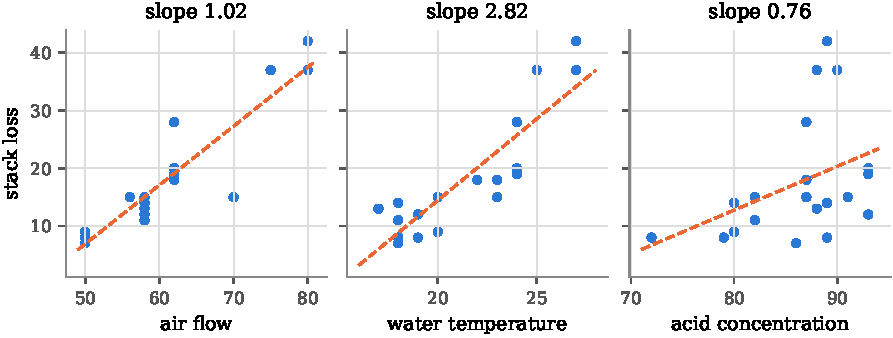
\includegraphics[width=\textwidth]{fig_mreg_predictors}
\caption{The stack loss data, $21$ days: the loss against the air flow, the cooling water temperature and the acid concentration, each with the least squares line of the loss on that predictor alone (orange, dashed).}
\label{fig:mregpredictors}
\end{figure}

With one predictor the model was $Y_i = a + bx_i + \epsilon_i$.
With three it is $Y_i = \beta_1 + \beta_2 x_{i2} + \beta_3 x_{i3} + \beta_4 x_{i4} + \epsilon_i$, and the natural way to write $n$ such equations is as one equation between vectors.

\begin{definition}[Linear regression model with several predictors]
\label{def:mreg-model}
Let $X$ be an $n \times p$ matrix of fixed numbers, the \textbf{design matrix}, whose row $i$ is $x_i^\top = (x_{i1}, \ldots, x_{ip})$, the $p$ predictor values of observation $i$; usually $x_{i1} = 1$ for every $i$, so that $\beta_1$ is the intercept.
The \textbf{linear regression model} says
\[
Y = X\beta + \epsilon, \qquad \text{that is,} \qquad Y_i = x_i^\top\beta + \epsilon_i, \quad i = 1, \ldots, n,
\]
for an unknown $\beta \in \real^p$, where $Y = (Y_1, \ldots, Y_n)^\top$ and the errors $\epsilon = (\epsilon_1, \ldots, \epsilon_n)^\top$ have mean $0$, a common variance $\sigma^2$ and no correlation: $\E[\epsilon] = 0$ and $\cov(\epsilon) = \sigma^2 I_n$.
The \textbf{Gaussian linear model} assumes moreover $\epsilon \sim \Gauss_n(0, \sigma^2 I_n)$, that is, $\epsilon_1, \ldots, \epsilon_n \iid \Gauss(0, \sigma^2)$.
\end{definition}

\begin{inwords}
Each response is a weighted sum of its predictor values, with the same weights $\beta$ for every observation, plus an error that behaves like every other error. The design matrix holds the data on the predictors, one row per observation and one column per predictor, and $X\beta$ is the vector of the $n$ means $\E[Y_i]$. The model of \cref{ch:regression-uni} is the case $p = 2$, with columns $(1, \ldots, 1)^\top$ and $(x_1, \ldots, x_n)^\top$ and $\beta = (a, b)^\top$.

\textbf{For the kiss data.} With no predictor the design matrix is the single column $(1, \ldots, 1)^\top$, $p = 1$, and $Y = X\beta + \epsilon$ says $R_i = p + \epsilon_i$: every couple has the same mean. A design with two columns, a column of ones and a column of $0$s and $1$s marking the couples observed in one of two cities, say, would let the mean differ between the cities, as the aspirin design of \cref{ex:reg-aspirin} let the heart-attack rate differ between the groups.
\end{inwords}

For the stack loss data, $n = 21$, $p = 4$, and row $1$ of $X$ is $(1, 80, 27, 89)$.
The model is linear in $\beta$, not necessarily in the measured variables, which is what makes it so general.
For Old Faithful, a design with columns $1$, $x_i$ and $x_i^2$ fits a parabola to the waits, and $x_i^2$ is simply a third column of numbers; a design with columns $1$, the duration and the previous wait lets the previous wait in; and a column of $0$s and $1$s, like the aspirin column of \cref{ex:reg-aspirin}, lets two groups have different means.
Treating the $x_i$ as fixed, and reading observational data through the conditional distribution of $Y$ given $X$, is as in \cref{sec:reg-model}.

\begin{remark}[The random-design version]
\Cref{ch:models} wrote the regression model with rows $x_i$ drawn from $\Gauss_d(0, I_d)$ and errors of variance $1$, as an example of a parametric model with $\Theta = \real^d$.
Condition on the drawn rows and that model is the Gaussian linear model of this chapter with $\sigma^2 = 1$ known; this chapter's $\Theta = \real^p \times (0, \infty)$ adds the unknown variance.
Every level and coverage statement below holds given the rows, and so, by the tower-property argument of \cref{sec:reg-model}, unconditionally as well; the distributions and moments themselves, such as $\cov(\hat{\beta}) = \sigma^2(X^\top X)^{-1}$, are statements given the rows.
\end{remark}

\section{Least squares in matrix form}
\label{sec:mreg-lse}

With one predictor, least squares minimized a sum of squared vertical distances.
In vector form that sum is the squared length of $Y - X\beta$, and minimizing a length is a problem in geometry.

\begin{definition}[Least squares estimator]
\label{def:mreg-lse}
The \textbf{least squares estimator} $\hat{\beta}$ minimizes the sum of squared errors
\[
\norm{Y - X\beta}^2 = \sum_{i=1}^n (Y_i - x_i^\top\beta)^2
\]
over $\beta \in \real^p$; the \textbf{fitted values} are $\hat{Y} = X\hat{\beta}$ and the \textbf{residuals} are $e = Y - \hat{Y}$.
\end{definition}

\begin{inwords}
Least squares picks, among all vectors of the form $X\beta$ (the column space of $X$ \toolkit{sec:math-matrices}), the one closest to the response vector $Y$ in ordinary Euclidean distance. The residuals are what is left over, observation by observation.

\textbf{For the kiss data.} With the single column of ones, $\norm{Y - X\beta}^2 = \sum_i (R_i - \beta)^2$ is smallest at $\beta = \bar{R}_n = 0.645$; the fitted vector is $0.645$ in every coordinate and the residuals are $0.355$ and $-0.645$ as in \cref{ch:regression-uni}.
\end{inwords}

The one-predictor theorem of \cref{ch:regression-uni} needed the $x_i$ not to be all equal.
The general condition is that the columns of $X$ be linearly independent: no column is a combination of the others, so that $X\beta = X\beta'$ only when $\beta = \beta'$, which is the statement that $X$ has rank $p$ \toolkit{sec:math-matrices}.

\begin{theorem}[The least squares estimator and the projection]
\label{thm:mreg-lse}
If $X$ has rank $p$, then $X^\top X$ is invertible and the least squares estimator is unique,
\[
\hat{\beta} = (X^\top X)^{-1}X^\top Y.
\]
The fitted vector is $\hat{Y} = PY$, with $P = X(X^\top X)^{-1}X^\top$ the matrix of the orthogonal projection onto the column space of $X$, and the residual vector $e = (I - P)Y$ is perpendicular to every column of $X$: $X^\top e = 0$.
\end{theorem}
\coreproof{The closest point to $Y$ in a subspace is the foot of the perpendicular, and the residual is perpendicular to the subspace. Perpendicular to every column means $X^\top(Y - X\hat{\beta}) = 0$, which are $p$ linear equations in $\hat{\beta}$ with the invertible matrix $X^\top X$.}
\begin{proof}
If $X^\top Xa = 0$ then $a^\top X^\top Xa = \norm{Xa}^2 = 0$, so $Xa = 0$ and, the columns being independent, $a = 0$: $X^\top X$ is invertible.
Let $\hat{\beta} = (X^\top X)^{-1}X^\top Y$ and $e = Y - X\hat{\beta}$.
Then $X^\top e = X^\top Y - X^\top X(X^\top X)^{-1}X^\top Y = 0$: the residual is perpendicular to the columns of $X$, hence to every vector $Xb$ in the column space.
For any $\beta$, write $Y - X\beta = e + X(\hat{\beta} - \beta)$, a sum of two perpendicular vectors, so by Pythagoras
\[
\norm{Y - X\beta}^2 = \norm{e}^2 + \norm{X(\hat{\beta} - \beta)}^2 \geq \norm{e}^2,
\]
with equality only when $X(\hat{\beta} - \beta) = 0$, that is, $\beta = \hat{\beta}$.
So $\hat{\beta}$ is the unique minimizer.
The matrix $P$ satisfies $P^\top = P$ and $P^2 = X(X^\top X)^{-1}X^\top X(X^\top X)^{-1}X^\top = P$, it fixes every vector in the column space ($PXb = Xb$) and sends every vector perpendicular to the columns to $0$, which is what the orthogonal projection does \toolkit{sec:math-matrices}; and $X\hat{\beta} = PY$ by the formula for $\hat{\beta}$.
\end{proof}

\Cref{fig:mregprojection} draws the theorem: the column space of $X$ as a plane through the origin, the response $Y$ as a vector above it, the fitted vector as the foot of the perpendicular from $Y$ to the plane, and the residual as the perpendicular itself.
Least squares is nothing but this picture, in $n$ dimensions.
The $p$ equations $X^\top e = 0$ are the \textbf{normal equations}; for the design with a column of ones and one predictor they are the two of \cref{thm:lse}, $\sum_i e_i = 0$ and $\sum_i x_ie_i = 0$.

\begin{figure}[htbp]
\centering
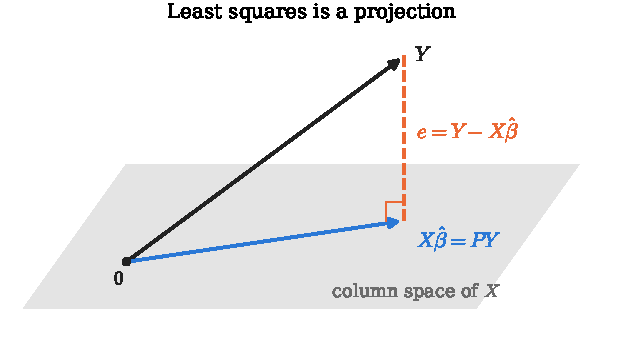
\includegraphics[width=0.62\textwidth]{fig_mreg_projection}
\caption{Least squares as a projection: the column space of $X$ (gray), the response vector $Y$ (black), the fitted vector $X\hat{\beta}$ (blue), the foot of the perpendicular from $Y$, and the residual $e$ (orange, dashed).}
\label{fig:mregprojection}
\end{figure}

\begin{worked}[the stack loss fit]
For the $21$ days, solving the normal equations gives
\[
\hat{\beta} = (-39.92,\ 0.716,\ 1.295,\ -0.152)^\top:
\]
in words, with the air flow, the water temperature and the acid concentration,
\[
\text{predicted loss} = -39.92 + 0.716\,(\text{air}) + 1.295\,(\text{water}) - 0.152\,(\text{acid}).
\]
Each unit of air flow adds $0.72$ to the loss when the other two are held fixed, each degree of water temperature adds $1.3$, and each unit of acid concentration subtracts $0.15$. The residual sum of squares is $\norm{e}^2 = 178.8$, against $\sum_i (Y_i - \bar{Y})^2 = 2{,}069.2$ for the constant fit, so the three predictors account for $1 - 178.8/2{,}069.2 = 91\%$ of the variation in the loss. \Cref{fig:mregstackloss} plots the observed losses against the fitted ones and the residuals against the fitted values; day $21$, with air flow $70$ and a loss of only $15$, is the worst-fitted day, with residual $-7.2$.
\end{worked}

\begin{figure}[htbp]
\centering
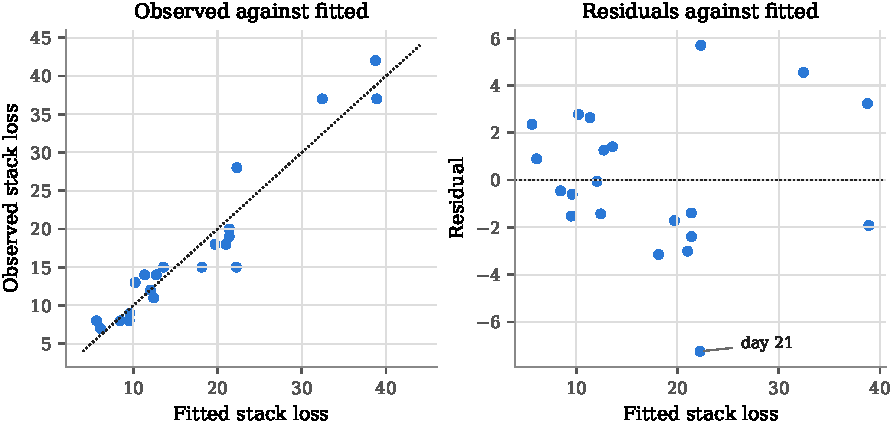
\includegraphics[width=\textwidth]{fig_mreg_stackloss}
\caption{The stack loss fit. Left: observed stack loss against the fitted values of the three-predictor model, with the line $y = x$ (dotted). Right: the residuals against the fitted values; day $21$ is the lowest point.}
\label{fig:mregstackloss}
\end{figure}

The coefficient $0.716$ is not the slope of the loss on the air flow alone, which \cref{fig:mregpredictors} drew, and the difference is the first thing to understand about a multiple regression.

\begin{sanitycheck}[A coefficient on its own, and in company]
Regress the loss on the air flow alone and the slope is $1.02$, not $0.72$. Both are right: $1.02$ is the change in loss per unit of air flow when the water temperature and the acid are left to vary as they did, and on these days warmer water went with higher air flow (correlation $0.78$), so the air flow alone gets credit for the water's effect as well. The multiple regression coefficient $0.72$ is the change per unit of air flow with the other two held fixed.
\end{sanitycheck}

When the columns of $X$ are dependent, the least squares problem still has a solution, the projection $PY$ onto the column space, but infinitely many $\beta$ produce it.

\needspace{12\baselineskip}
\begin{pitfall}[collinearity is non-identifiability]
If one column is a combination of the others, say $x_{i3} = 2x_{i2}$ for every $i$, then $X\beta = X\beta'$ whenever $\beta'$ moves weight from $\beta_2$ to $\beta_3$ in the ratio $2 : 1$. The distribution of $Y$ depends on $\beta$ only through $X\beta$, so two different parameters give the same distribution: the parameter is not identifiable, in the sense of \cref{ch:models}, and no data can tell $\beta$ from $\beta'$. Software reports it by dropping a column. A milder form appears when the columns are nearly dependent (\cref{sec:mreg-ttest}): $\hat{\beta}$ exists but has a large variance in the direction where the columns almost cancel.
\end{pitfall}

\section{The Gaussian linear model}
\label{sec:mreg-gaussian}

Everything \cref{ch:regression-uni} proved for one predictor holds for $p$, with $(X^\top X)^{-1}$ where $1/S_{xx}$ was.
The tool is the general form of Cochran's theorem, promised in \cref{ch:t-test}.

\begin{proposition}[Cochran's theorem, general form]
\label{prop:cochran-general}
Let $\epsilon \sim \Gauss_n(0, \sigma^2I_n)$, and let $\real^n$ be split into mutually perpendicular subspaces $S_1, \ldots, S_m$ of dimensions $d_1 + \cdots + d_m = n$, with orthogonal projections $P_1, \ldots, P_m$.
Then $\norm{P_1\epsilon}^2/\sigma^2, \ldots, \norm{P_m\epsilon}^2/\sigma^2$ are independent, with $\norm{P_j\epsilon}^2/\sigma^2 \sim \chi^2_{d_j}$.
\end{proposition}
\coreproof{Rotate to an orthonormal basis adapted to the subspaces, $d_1$ vectors spanning $S_1$, then $d_2$ spanning $S_2$, and so on. The rotated coordinates are independent $\Gauss(0, \sigma^2)$, and each $\norm{P_j\epsilon}^2$ is the sum of the squares of its own block of them.}
\begin{proof}
Choose an orthonormal basis of each $S_j$ and put them together: since the subspaces are perpendicular and their dimensions add to $n$, these are $n$ orthonormal vectors, and orthonormal vectors are linearly independent (dotting $\sum_k c_ku_k = 0$ with $u_j$ gives $c_j = 0$), so they are an orthonormal basis $u_1, \ldots, u_n$ of $\real^n$.
Let $Q$ be the orthogonal matrix with rows $u_k^\top$ and $Z = Q\epsilon$, so $Z_k = u_k^\top\epsilon$ and $\epsilon = \sum_k Z_ku_k$; by rotation invariance \toolkit{sec:math-gaussvec}, $Z_1, \ldots, Z_n$ are i.i.d.\ $\Gauss(0, \sigma^2)$.
The projection $P_j$ keeps the terms of $\sum_k Z_ku_k$ whose $u_k$ lie in $S_j$ and kills the rest, so $\norm{P_j\epsilon}^2$ is the sum of $Z_k^2$ over the $d_j$ indices of that block.
The blocks are disjoint, so the $m$ sums are independent, and each divided by $\sigma^2$ is a sum of $d_j$ squared independent standard Gaussians.
\end{proof}

\Cref{thm:cochran} is the case $m = 2$ with $S_1$ the line through $(1, \ldots, 1)$; the proofs below use $m = 2$ and $m = 3$ with the column space of $X$ in place of the line.

\begin{theorem}[Least squares with $p$ predictors]
\label{thm:mreg-exact}
In the linear regression model with $X$ of rank $p$ and $n > p$:
\begin{enumerate}[nosep]
\item $\E[\hat{\beta}] = \beta$ and $\cov(\hat{\beta}) = \sigma^2(X^\top X)^{-1}$, so the quadratic risk is $\E\norm{\hat{\beta} - \beta}^2 = \sigma^2\,\mathrm{tr}\big((X^\top X)^{-1}\big)$;
\item $\E\norm{e}^2 = (n - p)\sigma^2$, so $\hat{\sigma}^2 = \norm{e}^2/(n - p)$ is an unbiased estimator of $\sigma^2$.
\end{enumerate}
In the Gaussian linear model, moreover:
\begin{enumerate}[nosep]
\setcounter{enumi}{2}
\item $\hat{\beta} \sim \Gauss_p\big(\beta, \sigma^2(X^\top X)^{-1}\big)$, and the maximum likelihood estimators are $\hat{\beta}$ and $\norm{e}^2/n$;
\item $(n - p)\hat{\sigma}^2/\sigma^2 \sim \chi^2_{n-p}$, independent of $\hat{\beta}$;
\item for each $j$, with $\gamma_j$ the $j$th diagonal entry of $(X^\top X)^{-1}$,
\[
\frac{\hat{\beta}_j - \beta_j}{\hat{\sigma}\sqrt{\gamma_j}} \sim t_{n-p}.
\]
\end{enumerate}
\end{theorem}
\coreproof{$\hat{\beta} - \beta$ is a fixed matrix times the error vector, which gives the mean and covariance at once. For the residuals, rotate the errors so that the first $p$ axes span the column space: the fit absorbs those $p$ coordinates and the residual is the other $n - p$, which is \cref{prop:cochran-general} with the column space and its orthogonal complement.}
\recall{The chi-squared distribution (\cref{def:chisq}): a sum of $k$ squared independent standard Gaussians is $\chi^2_k$. Student's distribution (\cref{def:student}): if $Z \sim \Gauss(0, 1)$ and $V \sim \chi^2_k$ are independent, $Z/\sqrt{V/k} \sim t_k$. A Gaussian vector (\cref{sec:math-gaussquad}): if $W \sim \Gauss_n(0, \sigma^2 I_n)$ and $B$ is a $p \times n$ matrix of rank $p$, then $BW \sim \Gauss_p(0, \sigma^2 BB^\top)$.}
\begin{proof}
Substituting $Y = X\beta + \epsilon$ into the formula for $\hat{\beta}$,
\[
\hat{\beta} = (X^\top X)^{-1}X^\top(X\beta + \epsilon) = \beta + B\epsilon, \qquad B = (X^\top X)^{-1}X^\top,
\]
so $\E[\hat{\beta}] = \beta$ and $\cov(\hat{\beta}) = B\,\cov(\epsilon)\,B^\top = \sigma^2(X^\top X)^{-1}X^\top X(X^\top X)^{-1} = \sigma^2(X^\top X)^{-1}$ \toolkit{sec:math-gaussquad}.
The risk is $\E\norm{\hat{\beta} - \beta}^2 = \sum_j \var(\hat{\beta}_j)$, the sum of the diagonal entries of the covariance matrix, which is (1).

For (2), rotate.
By Gram--Schmidt \toolkit{sec:math-gaussvec} there is an orthonormal basis $u_1, \ldots, u_n$ of $\real^n$ whose first $p$ vectors span the column space of $X$; let $Q$ be the orthogonal matrix with rows $u_k^\top$ and set $Z = Q\epsilon$, so $Z_k = u_k^\top\epsilon$ and $\epsilon = \sum_k Z_ku_k$.
The $Z_k$ have mean $0$, variance $\sigma^2$ and are uncorrelated, since $\E[Z_jZ_k] = u_j^\top\cov(\epsilon)u_k = \sigma^2u_j^\top u_k$.
The projection $P$ fixes $u_1, \ldots, u_p$ and kills $u_{p+1}, \ldots, u_n$, so
\[
e = (I - P)Y = (I - P)(X\beta + \epsilon) = (I - P)\epsilon = \sum_{k=p+1}^n Z_ku_k, \qquad \norm{e}^2 = Z_{p+1}^2 + \cdots + Z_n^2,
\]
whose mean is $(n - p)\sigma^2$.
Likewise $\hat{\beta} - \beta = B\epsilon = B\sum_{k \leq p} Z_ku_k$, since $Bu_k = (X^\top X)^{-1}X^\top u_k = 0$ for $k > p$ ($u_k$ is perpendicular to the columns): $\hat{\beta}$ is a function of $Z_1, \ldots, Z_p$ alone.

With Gaussian errors, $Z/\sigma = Q(\epsilon/\sigma)$ has i.i.d.\ $\Gauss(0, 1)$ coordinates by rotation invariance \toolkit{sec:math-gaussvec}.
Then $\hat{\beta} = \beta + B\epsilon$ is Gaussian with the covariance of (1), since $B$ has rank $p$ (its $p$ rows are independent because $BX = I_p$); the log-likelihood is $-\frac{n}{2}\log(2\pi\sigma^2) - \norm{Y - X\beta}^2/(2\sigma^2)$, largest in $\beta$ where the sum of squares is smallest, so the maximum likelihood estimator of $\beta$ is $\hat{\beta}$, and then, as in \cref{prop:lse-mle}, its derivative in $\sigma^2$ at $\hat{\beta}$ is $-n/(2\sigma^2) + \norm{e}^2/(2\sigma^4)$, zero at $\sigma^2 = \norm{e}^2/n$: this is (3).
$(n - p)\hat{\sigma}^2/\sigma^2 = \sum_{k > p}(Z_k/\sigma)^2$ is $\chi^2_{n-p}$ by \cref{prop:cochran-general} with $S_1$ the column space and $S_2$ its orthogonal complement, and it is a function of $Z_{p+1}, \ldots, Z_n$ while $\hat{\beta}$ is a function of $Z_1, \ldots, Z_p$, so the two are independent: this is (4).
Finally $(\hat{\beta}_j - \beta_j)/(\sigma\sqrt{\gamma_j})$ is a standard Gaussian, independent of the $\chi^2_{n-p}$ variable of (4); dividing by $\sqrt{\hat{\sigma}^2/\sigma^2}$ gives $t_{n-p}$, which is (5).
\end{proof}

The fit takes $p$ dimensions and the residual the other $n - p$, which is why the divisor is $n - p$: $n - 1$ for a mean, $n - 2$ for a line, $17$ for the stack loss fit.

\begin{worked}[standard errors for the stack loss coefficients]
$\hat{\sigma} = \sqrt{178.8/17} = 3.24$, and the diagonal of $(X^\top X)^{-1}$ is $(13.45, 0.00173, 0.0129, 0.00232)$, so the standard errors $\hat{\sigma}\sqrt{\gamma_j}$ are $11.9$, $0.135$, $0.368$ and $0.156$. The $95\%$ confidence interval for the air flow coefficient is $0.716 \pm 2.110 \times 0.135 = [0.43, 1.00]$, with $q_{0.025}(t_{17}) = 2.110$; for the water temperature, $[0.52, 2.07]$; for the acid, $[-0.48, 0.18]$, which contains $0$. The quadratic risk of $\hat{\beta}$ is $\sigma^2 \times 13.47$, almost all of it from the intercept, whose variance is large because the predictors are far from $0$: air flow averages $60$, so the height of the fitted plane at air flow $0$ is an extrapolation.
\end{worked}

\section{One coefficient at a time}
\label{sec:mreg-ttest}

Part (5) of \cref{thm:mreg-exact} gives the test of \cref{ch:regression-uni} for every coefficient.
In the Gaussian linear model, the test of $H_0: \beta_j = 0$ against $H_1: \beta_j \neq 0$ that rejects when
\[
\abs{T_j} > q_{\alpha/2}(t_{n-p}), \qquad T_j = \frac{\hat{\beta}_j}{\hat{\sigma}\sqrt{\gamma_j}},
\]
has level exactly $\alpha$.
Its null hypothesis says that predictor $j$ adds nothing to a model that already contains the other $p - 1$.

\begin{worked}[which predictors matter for the stack loss]
$T = 5.31$ for the air flow and $3.52$ for the water temperature, both beyond $2.110$, with $p$-values $0.0001$ and $0.003$; $T = -0.97$ for the acid concentration, $p$-value $0.34$. Given the air flow and the water temperature, the acid concentration adds nothing that $21$ days can detect. Dropping it gives the fit $-50.36 + 0.671\,(\text{air flow}) + 1.295\,(\text{water temperature})$, with residual sum of squares $188.8$ against $178.8$.
\end{worked}

The sanity check of \cref{sec:mreg-lse} already showed that a coefficient depends on the company it keeps.
Old Faithful shows something stronger: two predictors can each look useless on its own and be useful together.

\begin{worked}[the previous eruption]
Fit, for the $271$ eruptions that have a predecessor, the wait on the duration and the previous wait: the previous wait's coefficient is $-0.058$ with $T = -1.82$, $p$-value $0.07$. Fit the wait on the duration and the previous duration instead: $T = 0.62$. Each, added alone to the line of \cref{ch:regression-uni}, falls short of $q_{0.025}(t_{268}) = 1.969$. Now add both: the coefficients are $-0.283$ for the previous wait ($T = -4.75$) and $3.12$ for the previous duration ($T = 4.40$), both far past the threshold, and $\hat{\sigma}$ drops from $5.91$ to $5.69$. The reason is that the previous wait and the previous duration have correlation $0.90$ (long eruptions are followed by long waits), so each stands in for the other when it is alone, and what the pair uses is the previous wait's excess over what the previous duration predicts for it: $-0.283\,(\text{previous wait}) + 3.12\,(\text{previous duration}) = -0.283\,(\text{previous wait} - 11.0 \times \text{previous duration})$, so given the previous duration, a longer previous wait means a shorter wait now.
\end{worked}

\begin{figure}[htbp]
\centering
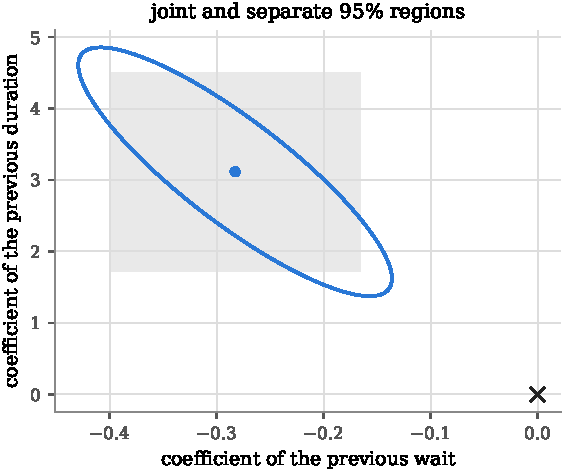
\includegraphics[width=0.52\textwidth]{fig_mreg_ellipse}
\caption{Old Faithful, the model with the duration, the previous wait and the previous duration: the joint $95\%$ confidence ellipse for the last two coefficients (blue), the two separate $95\%$ intervals (gray rectangle), the estimates (dot) and the origin (cross).}
\label{fig:mregellipse}
\end{figure}

\Cref{fig:mregellipse} draws the joint $95\%$ confidence region for the two coefficients in the full model, the ellipse $\{b : (\hat{b} - b)^\top C^{-1}(\hat{b} - b) \leq 2q_{0.05}(F_{2, 267})\}$ with $C$ the $2 \times 2$ block of $\hat{\sigma}^2(X^\top X)^{-1}$ (\cref{ex:mreg-ellipse}), together with the two separate intervals.
The ellipse is long and tilted, from upper left to lower right. Raise the previous wait's coefficient by $t$, lower the previous duration's by $11t$ and the intercept by $33t$, and the fitted values barely move, since the previous wait is close to $33 + 11 \times$ the previous duration, so the three columns nearly cancel in that combination; the data leave it loose, and it is the long axis of the ellipse. The combination along the short axis, $11$ times the previous wait's coefficient plus the previous duration's, is pinned down far better than either coefficient alone: its standard error is $0.37$, against $0.71$ for the previous duration's coefficient.
It is a mild form of the collinearity pitfall.
The origin lies far outside the ellipse, so the pair is clearly needed, and \cref{sec:mreg-ftest} gives the test that says so in one number.

\begin{pitfall}[what a coefficient does not say]
$\beta_j$ is the change in $\E[Y]$ per unit of predictor $j$ with the others held fixed, in a model containing exactly those others. It is not the effect of changing predictor $j$: the stack loss plant was observed, not manipulated, and the days with high air flow may have differed in ways the three columns do not record. A regression shows how the response moves with the predictors in the data; an experiment that sets the predictors, as the Physicians' Health Study of \cref{ex:reg-aspirin} assigned aspirin by randomization, is what shows what changing them does.
\end{pitfall}

\section{Several coefficients at once: the \texorpdfstring{$F$}{F}-test}
\label{sec:mreg-ftest}

`Does the acid concentration matter?' is one coefficient; `do the water temperature and the acid concentration matter, given the air flow?' is two.
Testing them one at a time at level $\alpha$ each does not give a test of level $\alpha$ for the pair, as \cref{ch:t-test} explained for many tests at once, and the previous worked example shows the stakes: there, both single tests failed and the pair was decisive.
The right test compares the fit with the predictors in question to the fit without them.

Let $X_0$ consist of the first $p - k$ columns of $X$, the predictors not under test, and let $\norm{e_0}^2$ be the residual sum of squares of the least squares fit with $X_0$ alone; it is at least $\norm{e}^2$, since the smaller model is a special case of the larger.

\begin{theorem}[The $F$-test]
\label{thm:mreg-ftest}
In the Gaussian linear model with $X$ of rank $p$, test $H_0: \beta_{p-k+1} = \cdots = \beta_p = 0$ against the alternative that at least one of them is not $0$.
Under $H_0$,
\[
F = \frac{(\norm{e_0}^2 - \norm{e}^2)/k}{\norm{e}^2/(n - p)} \sim F_{k, n-p},
\]
the $F$ distribution of \cref{ch:t-test}, so the test that rejects when $F > q_\alpha(F_{k, n-p})$ has level exactly $\alpha$.
It is the likelihood ratio test of \cref{ch:wald-lrt}: $T^{\mathrm{LR}}_n = n\log(\norm{e_0}^2/\norm{e}^2)$, an increasing function of $F$.
For $k = 1$, $F = T_p^2$, and the $F$-test is the two-sided $t$-test.
\end{theorem}
\coreproof{Split the error vector along three orthogonal subspaces: the column space of $X_0$, the part of the column space of $X$ perpendicular to it ($k$ dimensions), and the residual space ($n - p$ dimensions). Under $H_0$ the numerator is the squared length of the middle piece and the denominator that of the last; Cochran makes them independent chi-squareds.}
\begin{proof}
Let $P_0$ be the projection onto the column space of $X_0$ and $P$ onto that of $X$; the first space is inside the second, so $PP_0 = P_0$ and $P - P_0$ is the projection onto the part of the column space of $X$ perpendicular to the column space of $X_0$, a subspace of dimension $p - (p - k) = k$ \toolkit{sec:math-matrices}.
Then $e_0 = (I - P_0)Y$, $e = (I - P)Y$, and since $(I - P_0) = (P - P_0) + (I - P)$ with the two pieces perpendicular, Pythagoras gives
\[
\norm{e_0}^2 - \norm{e}^2 = \norm{(P - P_0)Y}^2.
\]
Under $H_0$, $X\beta = X_0\beta_0$ lies in the column space of $X_0$, so $(P - P_0)X\beta = 0$ and $(I - P)X\beta = 0$: both pieces are the same projections of $\epsilon$ alone.
Choose the orthonormal basis of the proof of \cref{thm:mreg-exact} so that $u_1, \ldots, u_{p-k}$ span the column space of $X_0$ and $u_1, \ldots, u_p$ that of $X$ (Gram--Schmidt applied to the columns of $X_0$ first, then the rest).
With $Z = Q\epsilon$ as before, $\norm{(P - P_0)\epsilon}^2 = Z_{p-k+1}^2 + \cdots + Z_p^2$ and $\norm{(I - P)\epsilon}^2 = Z_{p+1}^2 + \cdots + Z_n^2$: by \cref{prop:cochran-general} with the three subspaces, these are $\sigma^2$ times independent $\chi^2_k$ and $\chi^2_{n-p}$ variables, and the ratio of each to its degrees of freedom is $F_{k, n-p}$ by \cref{ch:t-test}'s definition.

For the likelihood ratio, the maximized log-likelihood of a Gaussian linear model is, by (3) of \cref{thm:mreg-exact}, $-\frac{n}{2}\log(2\pi\hat{\sigma}^2_{\mathrm{MLE}}) - \frac{n}{2}$ with $\hat{\sigma}^2_{\mathrm{MLE}} = \norm{e}^2/n$; the difference of the two models' maxima, times $2$, is $n\log(\norm{e_0}^2/\norm{e}^2) = n\log(1 + kF/(n - p))$, increasing in $F$.
For $k = 1$ the $k$-dimensional piece is one coordinate, $Z_p = u_p^\top\epsilon$, and under $H_0$, $\hat{\beta}_p = \sqrt{\gamma_p}\,Z_p$ (\cref{ex:mreg-t-f}), so $F = Z_p^2/\hat{\sigma}^2 = \hat{\beta}_p^2/(\gamma_p\hat{\sigma}^2) = T_p^2$; \cref{ex:mreg-t-f} shows that $F = T_p^2$ holds whether or not $H_0$ is true.
\end{proof}

\begin{worked}[two $F$-tests for the stack loss]
Do the three predictors together do anything? With $X_0$ the column of ones, $\norm{e_0}^2 = 2{,}069.2$, so
\[
F = \frac{(2{,}069.2 - 178.8)/3}{178.8/17} = \frac{630.1}{10.52} = 59.9
\]
on $(3, 17)$ degrees of freedom, against $q_{0.05}(F_{3, 17}) = 3.20$: $p$-value $3 \times 10^{-9}$. Do the water temperature and the acid add anything to the air flow? The fit on the air flow alone has $\norm{e_0}^2 = 319.1$, so $F = (319.1 - 178.8)/2 \div 10.52 = 70.2/10.52 = 6.67$ on $(2, 17)$ against $3.59$: $p$-value $0.007$, so of $1{,}000$ plants on which the water and the acid did nothing, about $7$ would give an $F$ this large. For Old Faithful, adding the previous wait and the previous duration to the duration gives $F = 11.5$ on $(2, 267)$, $p$-value $2 \times 10^{-5}$, where the two single $t$-tests found nothing.
\end{worked}

Any $k$ independent linear constraints on $\beta$, such as $\beta_2 = \beta_3$, take this form after a change of columns (with columns $x_2 + x_3$ and $x_3$ in place of $x_2$ and $x_3$, the coefficients are $\beta_2$ and $\beta_3 - \beta_2$), so the $F$-test covers the implicit hypotheses of \cref{ch:wald-lrt} as well.
Wilks' theorem (\cref{ch:wald-lrt}) would make $T^{\mathrm{LR}}_n$ approximately $\chi^2_k$; here Cochran's theorem makes $F$ exactly $F_{k, n-p}$, and as $n \to \infty$ with $k$ fixed, $kF \convd \chi^2_k$ (\cref{ex:mreg-f-chisq}), so the two agree in the limit.

\begin{bridge}[the ANOVA table and $R^2$]
Regression output's analysis-of-variance table is the first $F$-test above: the regression sum of squares $\norm{e_0}^2 - \norm{e}^2 = \sum_i (\hat{Y}_i - \bar{Y})^2$ on $p - 1$ degrees of freedom, the residual sum of squares on $n - p$, their mean squares, and their ratio $F$. Its $R^2 = 1 - \norm{e}^2/\norm{e_0}^2$ is the share of $\sum_i (Y_i - \bar{Y})^2$ that the fit accounts for ($0.914$ for the stack loss), and $F = \frac{R^2/(p - 1)}{(1 - R^2)/(n - p)}$ is the same number read off $R^2$. Adding a column never lowers $R^2$, since the larger model contains the smaller, which is why a high $R^2$ with many predictors proves little and the $F$-test, which charges each added column its degree of freedom, is the honest comparison.
\end{bridge}

\begin{remark}[Bonferroni's test]
An alternative to the $F$-test rejects $H_0$ when any one of the $k$ single tests rejects at level $\alpha/k$: by the union bound of \cref{prop:bonferroni}, its level is at most $\alpha$. For the water temperature and the acid, $\alpha/2 = 0.025$ gives the threshold $q_{0.0125}(t_{17}) = 2.458$, and $T = 3.52$ for the water rejects. Bonferroni does not need the $k$ tests to come from one model or one data set, and when it rejects it says which hypothesis failed, which the $F$-test does not; its price is the conservative level, and a case like Old Faithful's two predictors, where each single $T$ is small in its own smaller model, is exactly where it can miss what the $F$-test sees.
\end{remark}

\section{Ridge in matrix form}
\label{sec:mreg-ridge}

\Cref{ch:regression-uni} shrank one slope toward $0$ by adding a Gaussian prior; with $p$ coefficients the same prior on each gives the matrix form.
Under the Gaussian linear model with $\sigma^2$ known and the prior $\beta \sim \Gauss_p(0, \tau^2 I_p)$, the log posterior density is, up to a constant,
\[
-\frac{1}{2\sigma^2}\norm{Y - X\beta}^2 - \frac{1}{2\tau^2}\norm{\beta}^2,
\]
whose gradient in $\beta$ \toolkit{sec:math-multivar} is $\sigma^{-2}(X^\top Y - X^\top X\beta) - \tau^{-2}\beta$, zero at the \textbf{ridge estimator}
\[
\tilde{\beta}_\lambda = (X^\top X + \lambda I_p)^{-1}X^\top Y, \qquad \lambda = \frac{\sigma^2}{\tau^2},
\]
which minimizes $\norm{Y - X\beta}^2 + \lambda\norm{\beta}^2$.

\begin{figure}[htbp]
\centering
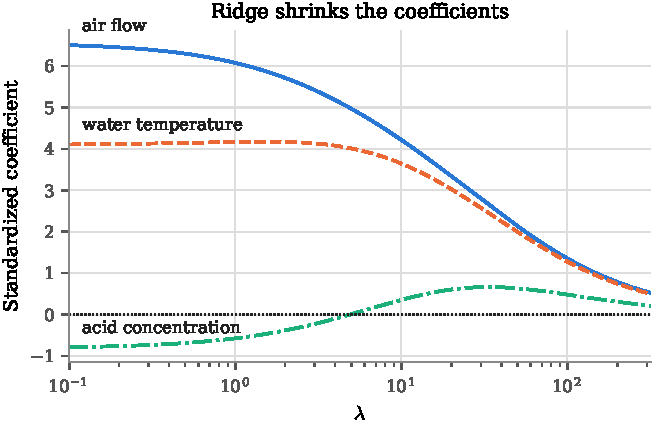
\includegraphics[width=0.72\textwidth]{fig_mreg_ridge}
\caption{Ridge on the stack loss data with standardized predictors: the coefficients of the air flow (blue), the water temperature (orange, dashed) and the acid concentration (aqua, dash-dot) against $\lambda$ on a logarithmic axis.}
\label{fig:mregridge}
\end{figure}

Since $a^\top(X^\top X + \lambda I)a = \norm{Xa}^2 + \lambda\norm{a}^2 > 0$ for $a \neq 0$ and $\lambda > 0$, the matrix is invertible whatever the rank of $X$: ridge has a unique answer even for collinear columns, where least squares has infinitely many, and a steady one when they are nearly collinear.
In practice the intercept is left out of the penalty and the predictors are standardized first, so that one $\lambda$ treats them alike.
\Cref{fig:mregridge} does this for the stack loss data: as $\lambda$ grows the three standardized coefficients leave their least squares values $(6.56, 4.09, -0.82)$, the air flow's and the water temperature's shrinking toward $0$ and the acid's, whose sign is not even determined by the data, crossing $0$ near $\lambda = 5$ before it too heads to $0$.
Choosing $\lambda$ is choosing $\tau$, the prior spread of the coefficients, and \cref{ex:reg-ridge} showed why a small positive $\lambda$ lowers the risk whatever $\beta$ is.

\section{Without Gaussian errors, and checking the model}
\label{sec:mreg-robust}

Nothing in parts (1) and (2) of \cref{thm:mreg-exact} needed Gaussian errors, and the large-sample theory of \cref{thm:lse-asymptotic} extends to $p$ predictors by the same route, with vectors in place of numbers.

\begin{theorem}[Least squares with $p$ predictors, without Gaussian errors]
\label{thm:mreg-asymptotic}
Let $(x_1, Y_1), (x_2, Y_2), \ldots$ be i.i.d.\ copies of $(x, Y) \in \real^p \times \real$ with finite fourth moments, let $M = \E[xx^\top]$ be positive definite, let $\beta^*$ minimize $\E[(Y - x^\top\beta)^2]$ and $\epsilon = Y - x^\top\beta^*$, and let $V = \E[\epsilon^2xx^\top]$ be positive definite.
Then $\hat{\beta} \convp \beta^*$ and
\[
\sqrt{n}(\hat{\beta} - \beta^*) \convd \Gauss_p(0, M^{-1}VM^{-1}).
\]
If $\E[\epsilon^2 \mid x] = \sigma^2$, then $M^{-1}VM^{-1} = \sigma^2M^{-1}$, $\hat{\sigma}^2 \convp \sigma^2$, and each $T_j$ of \cref{sec:mreg-ttest} converges in distribution to $\Gauss(0, 1)$ under $\beta_j^* = 0$.
\end{theorem}
\optionalproof{The one-predictor proof with matrices: $\hat{\beta} - \beta^* = (\frac1n X^\top X)^{-1}\frac1n X^\top\epsilon$, the Law of Large Numbers for the first factor and the vector Central Limit Theorem for the second.}
\recall{The Law of Large Numbers (\cref{thm:wlln}) for each entry of an average of i.i.d.\ matrices with finite variances; the continuous mapping theorem (\cref{thm:cmt}) for the inverse, continuous at an invertible matrix; the Central Limit Theorem for vectors (the vector-versions remark of \cref{ch:limit-tools}): for i.i.d.\ vectors $W_i$ with mean $0$ and positive definite covariance $V$, $\sqrt{n}\,\bar{W}_n \convd \Gauss_p(0, V)$; Slutsky's theorem (\cref{thm:slutsky}), as \cref{ch:wald-lrt} uses it for vectors: if $A_n \convp A$, a fixed matrix, and $W_n \convd W$, then $(A_n - A)W_n \convp 0$ entry by entry and $A_nW_n \convd AW$.}
\begin{proof}
The minimizer $\beta^*$ solves $\E[x(Y - x^\top\beta)] = 0$, since the gradient of $\E[(Y - x^\top\beta)^2]$ is $-2\E[x(Y - x^\top\beta)] = -2(\E[xY] - M\beta)$, so $\beta^* = M^{-1}\E[xY]$ and $\E[x\epsilon] = 0$.
Writing $Y_i = x_i^\top\beta^* + \epsilon_i$ in the formula for $\hat{\beta}$,
\[
\hat{\beta} - \beta^* = \Big(\frac1n\sum_i x_ix_i^\top\Big)^{-1}\frac1n\sum_i x_i\epsilon_i.
\]
By the Law of Large Numbers, entry by entry, $\frac1n\sum_i x_ix_i^\top \convp M$ (finite fourth moments make the variances finite), so $X^\top X$ is invertible, and $\hat{\beta}$ defined, with probability tending to $1$; the inverse is continuous at $M$, so the first factor converges in probability to $M^{-1}$. The second is an average of i.i.d.\ vectors $W_i = x_i\epsilon_i$ with mean $0$ and covariance $V$, which is finite since $\epsilon$, a linear combination of $Y$ and the entries of $x$, has a finite fourth moment and $\epsilon^2\abs{x_jx_k} \leq \frac12(\epsilon^4 + x_j^2x_k^2)$; so it converges in probability to $0$, and $\sqrt{n}$ times it converges in distribution to $\Gauss_p(0, V)$.
Slutsky's theorem gives $\hat{\beta} \convp \beta^*$ and $\sqrt{n}(\hat{\beta} - \beta^*) \convd M^{-1}\Gauss_p(0, V) = \Gauss_p(0, M^{-1}VM^{-1})$, by the linear-map rule for Gaussian vectors \toolkit{sec:math-gaussquad}.
If $\E[\epsilon^2 \mid x] = \sigma^2$, then $V = \E[xx^\top\E[\epsilon^2 \mid x]] = \sigma^2M$ by taking out what is known and the tower property \toolkit{sec:math-condexp}, and $M^{-1}VM^{-1} = \sigma^2M^{-1}$.
For $\hat{\sigma}^2$, $e = \epsilon - X(\hat{\beta} - \beta^*)$ and $X^\top e = 0$ give $\norm{e}^2 = \norm{\epsilon}^2 - \norm{X(\hat{\beta} - \beta^*)}^2$, and $\frac1n\norm{X(\hat{\beta} - \beta^*)}^2 = (\hat{\beta} - \beta^*)^\top\frac1n X^\top X(\hat{\beta} - \beta^*) \convp 0$, so $\hat{\sigma}^2 = \frac{n}{n-p}\cdot\frac1n\norm{e}^2 \convp \E[\epsilon^2] = \sigma^2$, by the Law of Large Numbers for the $\epsilon_i^2$, whose variance is finite by the fourth moments.
Then $T_j = \sqrt{n}\hat{\beta}_j\big/\big(\hat{\sigma}\sqrt{n\gamma_j}\big)$, where $n\gamma_j$, the $j$th diagonal entry of $(\frac1n X^\top X)^{-1}$, converges in probability to that of $M^{-1}$, and Slutsky's theorem finishes it.
\end{proof}

So the $t$-tests and intervals keep their level for large $n$ whatever the errors' distribution, as long as the scatter is the same everywhere; when it is not, the sandwich $M^{-1}VM^{-1}$, estimated by plugging in $\frac1n\sum_i x_ix_i^\top$ and $\frac1n\sum_i e_i^2x_ix_i^\top$, gives the robust standard errors of \cref{ch:mom-mestimation}'s bridge, the $p$-predictor form of the one in \cref{ch:regression-uni}; as there, the consistency of the plug-in estimate is stated and not proved.
The $F$-test survives the same way: $kF \convd \chi^2_k$ under $H_0$ for constant scatter (\cref{ex:mreg-f-chisq}).

What the theory cannot do is tell you whether the model is any good, and the residuals are the place to look.
In the Gaussian linear model the residuals are the projection $(I - P)\epsilon$ of the errors, so they should look like mean-zero noise with no pattern against the fitted values or against any predictor: a curve in such a plot says that the mean is not linear, a fan says that the scatter changes with the mean.
The right of \cref{fig:mregstackloss} shows neither for the stack loss, apart from day $21$.
Whether the errors are Gaussian can be tested with the residuals in place of the errors: the Lilliefors test of \cref{ch:ks} on the $21$ stack loss residuals gives $D = 0.107$ against a $5\%$ threshold of $0.19$, no evidence against normality, with two caveats: the threshold is approximate, since the residuals are correlated and their variances differ (\cref{ex:mreg-projection}), and $n = 21$ has little power (\cref{sec:ks-lilliefors}).
For the exactness of the $t$- and $F$-tests at $n = 21$ that is what matters. At $n = 271$ Old Faithful's whole-minute waits are covered by \cref{thm:mreg-asymptotic}, but its rows are not independent, and in the model with the previous wait as a predictor they cannot be: the previous wait is the response of the row before. The $t$ and $F$ statistics for that model are the ones the Gaussian linear model prescribes, and large-sample theory for such lagged designs, which this book does not develop, supports them approximately, as the remarks of \cref{sec:reg-inference} did for consecutive eruptions.

\section{What comes next}
\label{sec:mreg-next}

This chapter closes Part VIII.
The response has been a number whose mean is linear in the predictors and whose scatter is the same everywhere.
For the kiss data's $0$s and $1$s, or for counts, neither holds: a mean that is a probability cannot be a line in the predictors without leaving $[0, 1]$, and the variance $p(1 - p)$ moves with the mean.
Part IX keeps the linear predictor $x^\top\beta$ and changes what it is linked to: \cref{ch:exp-families} describes the distributions for which this works, the exponential families, and \cref{ch:glm-links} links their means to $x^\top\beta$ through a function such as the log-odds of \cref{ch:jeffreys}, with maximum likelihood, now without a closed form, doing the fitting.

\section{Summary}
\label{sec:mreg-summary}

\begin{itemize}[nosep]
\item $Y = X\beta + \epsilon$ with an $n \times p$ design matrix, $\E[\epsilon] = 0$, $\cov(\epsilon) = \sigma^2I_n$; polynomials, $0/1$ variables and lagged values are columns like any other. Full rank of $X$ is identifiability; collinearity is its failure.
\item $\hat{\beta} = (X^\top X)^{-1}X^\top Y$ is unique when $X$ has rank $p$; $X\hat{\beta} = PY$ is the projection of $Y$ onto the column space, $e \perp$ every column (the normal equations $X^\top e = 0$). Stack loss: $-39.92 + 0.716\,\text{air} + 1.295\,\text{water} - 0.152\,\text{acid}$, $R^2 = 0.914$.
\item $\E[\hat{\beta}] = \beta$, $\cov(\hat{\beta}) = \sigma^2(X^\top X)^{-1}$, risk $\sigma^2\,\mathrm{tr}((X^\top X)^{-1})$; $\hat{\sigma}^2 = \norm{e}^2/(n - p)$ is unbiased. Gaussian errors: $\hat{\beta} \sim \Gauss_p(\beta, \sigma^2(X^\top X)^{-1})$ is the MLE, $(n - p)\hat{\sigma}^2/\sigma^2 \sim \chi^2_{n-p}$ independent of $\hat{\beta}$ (Cochran, general form), $(\hat{\beta}_j - \beta_j)/(\hat{\sigma}\sqrt{\gamma_j}) \sim t_{n-p}$.
\item One coefficient: $T_j = \hat{\beta}_j/(\hat{\sigma}\sqrt{\gamma_j})$ against $q_{\alpha/2}(t_{n-p})$; stack loss $T = 5.31, 3.52, -0.97$. A coefficient is a statement about a model: the air flow's $1.02$ alone, $0.72$ with the others; Old Faithful's previous wait and previous duration, useless alone and decisive together.
\item Several coefficients: $F = \frac{(\norm{e_0}^2 - \norm{e}^2)/k}{\norm{e}^2/(n - p)} \sim F_{k, n-p}$ under $H_0$, the likelihood ratio test made exact; $F = T^2$ for $k = 1$; stack loss $59.9$ on $(3, 17)$ and $6.67$ on $(2, 17)$; Old Faithful $11.5$ on $(2, 267)$. Bonferroni, $\alpha/k$ per test, has level at most $\alpha$ and says which hypothesis failed.
\item Ridge: $(X^\top X + \lambda I)^{-1}X^\top Y$, the posterior mode under $\beta \sim \Gauss_p(0, \tau^2I)$, $\lambda = \sigma^2/\tau^2$; defined for every $X$.
\item Without Gaussian errors, for i.i.d.\ rows: $\sqrt{n}(\hat{\beta} - \beta^*) \convd \Gauss_p(0, M^{-1}VM^{-1})$, which is $\sigma^2M^{-1}$ for constant scatter; the sandwich otherwise. Check the residuals against the fitted values, and their normality with Lilliefors.
\end{itemize}

\section{Exercises}
\label{sec:mreg-exercises}

\begin{exercise}
\label{ex:mreg-onepred}
Take $X$ with columns $(1, \ldots, 1)^\top$ and $(x_1, \ldots, x_n)^\top$. (a) Compute $X^\top X$, $X^\top Y$ and $(X^\top X)^{-1}$, and show that $\hat{\beta} = (X^\top X)^{-1}X^\top Y$ is the pair $(\hat{a}, \hat{b})$ of \cref{thm:lse}. (b) Show that $\sigma^2(X^\top X)^{-1}$ is the covariance matrix of \cref{prop:lse-moments}.
\end{exercise}
\begin{solution}
(a) $X^\top X = \begin{pmatrix} n & \sum_i x_i \\ \sum_i x_i & \sum_i x_i^2\end{pmatrix}$, $X^\top Y = (\sum_i Y_i, \sum_i x_iY_i)^\top$, and $\det(X^\top X) = n\sum_i x_i^2 - (\sum_i x_i)^2 = nS_{xx}$, so $(X^\top X)^{-1} = \frac{1}{nS_{xx}}\begin{pmatrix} \sum_i x_i^2 & -n\bar{x} \\ -n\bar{x} & n\end{pmatrix}$. The second row gives
\[
\hat{b} = \frac{n\sum_i x_iY_i - n\bar{x}\sum_i Y_i}{nS_{xx}} = \frac{S_{xy}}{S_{xx}}, \qquad \hat{a} = \frac{\sum_i x_i^2\sum_i Y_i - n\bar{x}\sum_i x_iY_i}{nS_{xx}} = \bar{Y} - \hat{b}\bar{x},
\]
the second after writing $\sum_i x_i^2 = S_{xx} + n\bar{x}^2$. (b) $\sigma^2$ times the entries: $\var(\hat{b}) = \sigma^2/S_{xx}$, $\var(\hat{a}) = \sigma^2\sum_i x_i^2/(nS_{xx}) = \sigma^2(1/n + \bar{x}^2/S_{xx})$, $\cov(\hat{a}, \hat{b}) = -\sigma^2\bar{x}/S_{xx}$.
\end{solution}

\begin{exercise}
\label{ex:mreg-groups}
Two groups. Let $X$ have a column of ones and a column $z$ of $0$s and $1$s, with $n_1$ ones and $n_0 = n - n_1$ zeros. (a) Compute $(X^\top X)^{-1}$ and show that $\hat{\beta} = (\bar{Y}_0, \bar{Y}_1 - \bar{Y}_0)^\top$. (b) Show that $\gamma_2 = 1/n_0 + 1/n_1$, so that $T_2$ is the pooled two-sample $t$ statistic of \cref{thm:pooled-t} and the $t$-test for $\beta_2 = 0$ is the pooled $t$-test. (c) In the aspirin study, $n_0 = 11{,}034$ and $n_1 = 11{,}037$; verify $\gamma_2$ and the standard error $0.00154$ of \cref{ex:reg-aspirin}.
\end{exercise}
\begin{solution}
(a) $X^\top X = \begin{pmatrix} n & n_1 \\ n_1 & n_1\end{pmatrix}$, with inverse $\frac{1}{nn_1 - n_1^2}\begin{pmatrix} n_1 & -n_1 \\ -n_1 & n\end{pmatrix} = \frac{1}{n_0}\begin{pmatrix} 1 & -1 \\ -1 & n/n_1\end{pmatrix}$, and $X^\top Y = (n_0\bar{Y}_0 + n_1\bar{Y}_1, n_1\bar{Y}_1)^\top$, giving $\hat{\beta}_1 = \bar{Y}_0$ and $\hat{\beta}_2 = \bar{Y}_1 - \bar{Y}_0$. (b) $\gamma_2 = n/(n_0n_1) = 1/n_0 + 1/n_1$, and $\hat{\sigma}^2$ is the pooled variance (the residuals are the deviations within each group, on $n - 2$ degrees of freedom), so $T_2 = (\bar{Y}_1 - \bar{Y}_0)/(\hat{\sigma}\sqrt{1/n_0 + 1/n_1})$. (c) $\gamma_2 = 1/11{,}034 + 1/11{,}037 = 1.8124 \times 10^{-4}$, and with $\hat{\sigma}^2 = 0.01309$ the standard error is $\sqrt{0.01309 \times 1.8124 \times 10^{-4}} = 0.00154$.
\end{solution}

\begin{exercise}
\label{ex:mreg-projection}
Let $P = X(X^\top X)^{-1}X^\top$ with $X$ of rank $p$. (a) Show that $\mathrm{tr}(P) = p$ and $\mathrm{tr}(I - P) = n - p$, using $\mathrm{tr}(AB) = \mathrm{tr}(BA)$. (b) Deduce $\E\norm{e}^2 = (n - p)\sigma^2$ directly from $e = (I - P)\epsilon$ and $\E[\epsilon\epsilon^\top] = \sigma^2I$, without the rotation. (c) The diagonal entry $P_{ii}$ is called the leverage of observation $i$; show that $\var(e_i) = \sigma^2(1 - P_{ii})$, so a high-leverage observation has a small residual however badly it fits. For the stack loss data the largest leverage is $0.41$, on day $17$, and $\mathrm{tr}(P) = 4$.
\end{exercise}
\begin{solution}
(a) $\mathrm{tr}(P) = \mathrm{tr}\big((X^\top X)^{-1}X^\top X\big) = \mathrm{tr}(I_p) = p$, and $\mathrm{tr}(I_n - P) = n - p$. (b) $\norm{e}^2 = \epsilon^\top(I - P)^\top(I - P)\epsilon = \epsilon^\top(I - P)\epsilon = \mathrm{tr}\big((I - P)\epsilon\epsilon^\top\big)$, whose expectation is $\mathrm{tr}\big((I - P)\sigma^2I\big) = (n - p)\sigma^2$. (c) $\cov(e) = (I - P)\sigma^2I(I - P)^\top = \sigma^2(I - P)$, so $\var(e_i) = \sigma^2(1 - P_{ii})$; as $P_{ii} \to 1$ the residual's variance vanishes, so the fit passes near the observation whatever its value.
\end{solution}

\begin{exercise}
\label{ex:mreg-t-f}
For $k = 1$ in \cref{thm:mreg-ftest}, show that $\norm{e_0}^2 - \norm{e}^2 = \hat{\beta}_p^2/\gamma_p$, so that $F = T_p^2$. (Write $u_p$, the last basis vector of the proof, as $(I - P_0)x_p/\norm{(I - P_0)x_p}$ with $x_p$ the last column of $X$, and use $\hat{\beta}_p = u_p^\top Y/\norm{(I - P_0)x_p}$ and $\gamma_p = 1/\norm{(I - P_0)x_p}^2$; the last two follow from writing the fit of the full model as the fit of $X_0$ plus the fit of the residual of $x_p$ on $X_0$.)
\end{exercise}
\begin{solution}
Let $w = (I - P_0)x_p$, the part of the last column perpendicular to the column space of $X_0$; $w \neq 0$ since $X$ has full rank, and the column space of $X$ is spanned by the columns of $X_0$ together with $w$, with $w$ perpendicular to the first. So $P = P_0 + ww^\top/\norm{w}^2$ and $(P - P_0)Y = (w^\top Y/\norm{w}^2)w$, whose squared length is $(w^\top Y)^2/\norm{w}^2$. The coefficient of $x_p$ in the full fit is the coefficient of $w$ in $PY$, since replacing $x_p$ by $w$ only reparameterizes the $X_0$ coefficients: $\hat{\beta}_p = w^\top Y/\norm{w}^2$, and its variance $\sigma^2\gamma_p$ is $\sigma^2\norm{w}^2/\norm{w}^4 = \sigma^2/\norm{w}^2$. Hence $\norm{e_0}^2 - \norm{e}^2 = \hat{\beta}_p^2\norm{w}^2 = \hat{\beta}_p^2/\gamma_p$ and $F = \hat{\beta}_p^2/(\hat{\sigma}^2\gamma_p) = T_p^2$. For the stack loss acid coefficient, $(188.8 - 178.8)/10.52 = 0.95 = (-0.973)^2$.
\end{solution}

\begin{exercise}
\label{ex:mreg-f-chisq}
(a) Show that if $V \sim \chi^2_k$ and $W_n \sim \chi^2_{n-p}$ are independent, then $k\,\frac{V/k}{W_n/(n - p)} \convd \chi^2_k$ as $n \to \infty$ with $k$ and $p$ fixed. (b) Explain why, under the hypotheses of \cref{thm:mreg-asymptotic} with constant scatter and $H_0$ true, $kF \convd \chi^2_k$ even without Gaussian errors. (Write $\norm{e_0}^2 - \norm{e}^2$ as a quadratic form in $\sqrt{n}(\hat{\beta} - \beta^*)$'s last $k$ coordinates.)
\end{exercise}
\begin{solution}
(a) $W_n/(n - p)$ is the mean of $n - p$ i.i.d.\ $\chi^2_1$ variables, which converges in probability to $1$ by the Law of Large Numbers, so $kF = V/(W_n/(n - p)) \convd V$ by Slutsky's theorem. (b) Let $X_1$ be the last $k$ columns of $X$, $\hat{\beta}_{(k)}$ their coefficients and $C_{(k)}$ the matching block of $(X^\top X)^{-1}$, and let $W = (I - P_0)X_1$, the parts of those columns perpendicular to the column space of $X_0$; $W$ has rank $k$ since $X$ has rank $p$, and $X_1 = X_0A + W$ for some matrix $A$. As in the previous exercise the column space of $X$ is that of $X_0$ plus that of $W$, perpendicular to each other, so $P = P_0 + W(W^\top W)^{-1}W^\top$; and $X\beta = X_0(\beta_0 + A\beta_{(k)}) + W\beta_{(k)}$ shows that $\hat{\beta}_{(k)} = (W^\top W)^{-1}W^\top Y$, with covariance $\sigma^2(W^\top W)^{-1}$, so $C_{(k)} = (W^\top W)^{-1}$. Hence $\norm{e_0}^2 - \norm{e}^2 = \norm{(P - P_0)Y}^2 = Y^\top W(W^\top W)^{-1}W^\top Y = \hat{\beta}_{(k)}^\top C_{(k)}^{-1}\hat{\beta}_{(k)}$. Under $H_0$, $\sqrt{n}\hat{\beta}_{(k)} \convd \Gauss_k(0, \sigma^2 M^{-1}_{(k)})$ and $nC_{(k)} \convp M^{-1}_{(k)}$ by \cref{thm:mreg-asymptotic}, so the quadratic form converges in distribution to $\sigma^2\chi^2_k$ by \cref{lem:gauss-quadform} and the continuous mapping theorem; dividing by $\hat{\sigma}^2 \convp \sigma^2$ gives $kF \convd \chi^2_k$.
\end{solution}

\begin{exercise}
\label{ex:mreg-ellipse}
Joint confidence region. In the Gaussian linear model let $\hat{\beta}_{(k)}$ and $C_{(k)}$ be as in the previous exercise, and let $\hat{C}_{(k)} = \hat{\sigma}^2C_{(k)}$. Show that $(\hat{\beta}_{(k)} - \beta_{(k)})^\top\hat{C}_{(k)}^{-1}(\hat{\beta}_{(k)} - \beta_{(k)})/k \sim F_{k, n-p}$, so that the ellipsoid $\{b : (\hat{\beta}_{(k)} - b)^\top\hat{C}_{(k)}^{-1}(\hat{\beta}_{(k)} - b) \leq k\,q_\alpha(F_{k, n-p})\}$ is a confidence region of level $1 - \alpha$ for $\beta_{(k)}$. This is the ellipse of \cref{fig:mregellipse}, with $k = 2$ and $2q_{0.05}(F_{2, 267}) = 6.06$.
\end{exercise}
\begin{solution}
$\hat{\beta}_{(k)} \sim \Gauss_k(\beta_{(k)}, \sigma^2C_{(k)})$ by the linear-map rule, so by \cref{lem:gauss-quadform} the quadratic form $(\hat{\beta}_{(k)} - \beta_{(k)})^\top(\sigma^2C_{(k)})^{-1}(\hat{\beta}_{(k)} - \beta_{(k)})$ is $\chi^2_k$, independent of $(n - p)\hat{\sigma}^2/\sigma^2 \sim \chi^2_{n-p}$ by \cref{thm:mreg-exact}. Replacing $\sigma^2$ by $\hat{\sigma}^2$ multiplies the quadratic form by $\sigma^2/\hat{\sigma}^2$, so the quantity in the exercise is $(\chi^2_k/k)/(\chi^2_{n-p}/(n - p))$ with independent numerator and denominator: $F_{k, n-p}$. The ellipsoid contains $\beta_{(k)}$ exactly when this statistic is at most $q_\alpha(F_{k, n-p})$, which has probability $1 - \alpha$.
\end{solution}

\begin{exercise}
\label{ex:mreg-quadratic}
Polynomial regression. For Old Faithful, fitting the waits on $1$, $x$ and $x^2$ gives $\hat{\beta} = (17.20, 22.21, -1.766)^\top$ with $T = -3.74$ for the squared term and residual sum of squares $8{,}976.7$, against $9{,}443.4$ for the line. (a) Compute the $F$ statistic for the squared term and check that it equals $T^2$. (b) The fitted parabola's slope at $x$ is $22.21 - 3.53x$; evaluate it at $2$ and at $4.5$ minutes and relate the numbers to the residual plot of \cref{fig:reglsfit}. (c) Why is this still a linear regression?
\end{exercise}
\begin{solution}
(a) $F = (9{,}443.4 - 8{,}976.7)/1 \div 8{,}976.7/269 = 466.7/33.37 = 13.99 = (-3.74)^2$. (b) $15.1$ minutes per minute at $2$ minutes and $6.3$ at $4.5$: the waits rise faster than the line for short eruptions and more slowly for long ones, which is the bend in the bin means of \cref{fig:reglsfit}. (c) The model is linear in the coefficients: $x^2$ is a column of numbers computed from the durations, and $Y = X\beta + \epsilon$ with that column is \cref{def:mreg-model}.
\end{solution}

\begin{exercise}
\label{ex:mreg-gm}
Gauss--Markov in general. In the linear regression model with $X$ of rank $p$, let $\tilde{\beta} = AY$ be any estimator that is linear in $Y$ and unbiased for every $\beta$. (a) Show that $AX = I_p$. (b) Write $A = (X^\top X)^{-1}X^\top + D$ and show that $DX = 0$. (c) Show that $\cov(\tilde{\beta}) = \sigma^2(X^\top X)^{-1} + \sigma^2DD^\top$, so that every coordinate of $\hat{\beta}$ has the smallest variance among linear unbiased estimators.
\end{exercise}
\begin{solution}
(a) $\E[AY] = AX\beta$ equals $\beta$ for every $\beta$ only if $AX = I_p$. (b) $DX = AX - (X^\top X)^{-1}X^\top X = I_p - I_p = 0$. (c) $\cov(AY) = \sigma^2AA^\top$, and $AA^\top = (X^\top X)^{-1}X^\top X(X^\top X)^{-1} + (X^\top X)^{-1}X^\top D^\top + DX(X^\top X)^{-1} + DD^\top$; the two middle terms vanish since $DX = 0$ and $(DX)^\top = X^\top D^\top = 0$. The diagonal of $DD^\top$ is $\sum_k D_{jk}^2 \geq 0$, so $\var(\tilde{\beta}_j) \geq \var(\hat{\beta}_j)$ for each $j$; this is \cref{prop:gauss-markov} for every coordinate at once.
\end{solution}

\begin{exercise}
\label{ex:mreg-ridge-bias}
For the ridge estimator with $X$ of rank $p$, (a) show that $\E[\tilde{\beta}_\lambda] = (X^\top X + \lambda I)^{-1}X^\top X\beta$, so it is biased for $\lambda > 0$, and that $\cov(\tilde{\beta}_\lambda) = \sigma^2(X^\top X + \lambda I)^{-1}X^\top X(X^\top X + \lambda I)^{-1}$; (b) when $X^\top X = cI_p$ (orthogonal columns of equal length), show that $\tilde{\beta}_\lambda = \frac{c}{c + \lambda}\hat{\beta}$, the one-predictor shrinkage of \cref{sec:reg-gauss} applied to every coordinate.
\end{exercise}
\begin{solution}
(a) $\tilde{\beta}_\lambda = (X^\top X + \lambda I)^{-1}X^\top(X\beta + \epsilon)$; the expectation is the first term and the covariance is $(X^\top X + \lambda I)^{-1}X^\top\,\sigma^2I\,X(X^\top X + \lambda I)^{-1}$. (b) $(cI + \lambda I)^{-1}X^\top Y = \frac{1}{c + \lambda}X^\top Y$ and $\hat{\beta} = \frac1cX^\top Y$, so $\tilde{\beta}_\lambda = \frac{c}{c + \lambda}\hat{\beta}$, which is the factor $S_{xx}/(S_{xx} + \lambda)$ with $c$ in place of $S_{xx}$.
\end{solution}

\begin{exercise}
\label{ex:mreg-kiss}
The kiss data as a regression. (a) With $X$ the column of ones, compute $(X^\top X)^{-1}$, $\hat{\beta}$, $P$ and $\mathrm{tr}(P)$. (b) Suppose the $124$ couples had been observed in two cities, $60$ in the first with $36$ right turns and $64$ in the second with $44$, and add the city as a $0/1$ column. Compute $\hat{\beta}$, $\norm{e}^2$, $\hat{\sigma}^2$ and $T_2$, and say what the test of $\beta_2 = 0$ asks. (c) Which assumption of the Gaussian linear model fails, and what makes the test usable anyway?
\end{exercise}
\begin{solution}
(a) $X^\top X = 124$, $(X^\top X)^{-1} = 1/124$, $\hat{\beta} = \bar{R}_n = 0.645$, $P$ is the matrix with every entry $1/124$, whose trace is $1$. (b) By \cref{ex:mreg-groups}, $\hat{\beta} = (36/60, 44/64 - 36/60)^\top = (0.600, 0.0875)^\top$; $\norm{e}^2 = 36(0.4)^2 + 24(0.6)^2 + 44(0.3125)^2 + 20(0.6875)^2 = 5.76 + 8.64 + 4.30 + 9.45 = 28.15$, $\hat{\sigma}^2 = 28.15/122 = 0.2307$, $\gamma_2 = 1/60 + 1/64 = 0.03229$, and $T_2 = 0.0875/\sqrt{0.2307 \times 0.03229} = 1.01$: no evidence that the proportion turning right differs between the cities. (c) The errors take two values, so they are not Gaussian, and their variance $p(1 - p)$ differs slightly between the cities ($0.240$ and $0.215$). With the couples modeled as i.i.d.\ draws whose city is recorded, \cref{thm:mreg-asymptotic} applies without its constant-scatter condition, and the robust standard error, here the unpooled $\sqrt{0.240/60 + 0.215/64} = 0.0858$, makes the test asymptotically valid; it is within $1\%$ of the pooled $\hat{\sigma}\sqrt{\gamma_2} = 0.0863$, as in \cref{ex:reg-aspirin}.
\end{solution}


\partintro{Regression for responses that are not Gaussian. Exponential families (\cref{ch:exp-families}) are the distributions the method works for; link functions and the fitting algorithm (\cref{ch:glm-links}) connect them to a linear predictor, with maximum likelihood doing the estimation as in Part IV.}
\part{Generalized Linear Models}
\chapter{Exponential Families}
\label{ch:exp-families}

% Not yet written. Source material: notes ch. Generalized Linear Models (exponential family, canonical form); unit 8 slides

\chapter[Link Functions and Fitting]{Generalized Linear Models: Link Functions and Fitting}
\label{ch:glm-links}

% Not yet written. Source material: unit 8 slides (nothing in the notes)


\partintro{The book's one chapter of unsupervised statistics: finding the directions in which multivariate data vary most, through the eigenvectors of the sample covariance matrix, and what the Law of Large Numbers says about them (\cref{ch:pca}).}
\part{Principal Component Analysis}
\chapter{Principal Component Analysis}
\label{ch:pca}

\begin{chaptergoals}
\begin{itemize}[nosep]
\item A sample of vectors as a cloud of points in $\real^d$: its mean vector and covariance matrix, and the sample variance of the cloud in a direction $u$, which is $u^\top Su$.
\item The direction of greatest spread is the first eigenvector of $S$, the next the second, and so on: the principal directions, proved from the spectral theorem.
\item Principal component analysis as the best flat picture of the cloud: the projection onto the first $k$ principal directions loses less than any other $k$-dimensional projection, and the eigenvalues say how much.
\item What the sample covariance estimates: $S \convp \Sigma$ entry by entry by the Law of Large Numbers, and the sample directions converge to the population's by the continuous mapping theorem. The units pitfall, and what happens when $d$ is not small against $n$.
\end{itemize}
Every chapter so far had one variable to explain or one parameter to estimate. This last chapter looks at many variables at once with no one of them singled out, and asks only in which directions they vary together.
\end{chaptergoals}

\section{A cloud of points}
\label{sec:pca-cloud}

The Old Faithful record of \cref{ch:regression-uni} has two numbers per eruption, its duration and the wait to the next one; the stack loss record of \cref{ch:regression-multi} has four per day.
Regression picked one of them as the response.
Drop that choice: each observation is a point $X_i \in \real^d$, the sample is a cloud of $n$ points, and the question is the cloud's shape.

\begin{definition}[Mean vector and covariance matrix]
\label{def:covmatrix}
Let $X = (X^{(1)}, \ldots, X^{(d)})^\top$ be a random vector with $\E[\norm{X}^2] < \infty$.
Its \textbf{mean vector} is $\E[X] = (\E[X^{(1)}], \ldots, \E[X^{(d)}])^\top$ and its \textbf{covariance matrix} is the $d \times d$ matrix
\[
\Sigma = \E\big[(X - \E[X])(X - \E[X])^\top\big], \qquad \Sigma_{jk} = \cov(X^{(j)}, X^{(k)}),
\]
with the variances on the diagonal.
For a sample $X_1, \ldots, X_n$ the \textbf{sample mean vector} is $\bar{X} = \frac1n\sum_i X_i$ and the \textbf{sample covariance matrix} is
\[
S = \frac1n\sum_{i=1}^n (X_i - \bar{X})(X_i - \bar{X})^\top,
\]
whose $(j, k)$ entry is the sample covariance of the $j$th and $k$th coordinates, with divisor $n$.
\end{definition}

\begin{inwords}
The mean vector is the center of the cloud and the covariance matrix its shape: each diagonal entry is the spread along one axis, each off-diagonal entry says whether two coordinates move together. The sample versions are the same averages over the points. With $\mathbf{X}$ the $n \times d$ matrix whose rows are the $X_i^\top$ (the design matrix of \cref{ch:regression-multi}, in bold here because $X$ is the random vector), $\bar{X} = \frac1n\mathbf{X}^\top\mathbf{1}$ and $S = \frac1n\mathbf{X}^\top H\mathbf{X}$ with $H = I - \frac1n\mathbf{1}\mathbf{1}^\top$ the projection that removes the column means.

\textbf{For the kiss data.} With $d = 1$ the vector is the single $0/1$ variable $R_i$, the mean vector is $\hat{p} = 0.645$ and the covariance matrix is the one number $\hat{p}(1 - \hat{p}) = 0.229$, the sample variance with divisor $n$ (\cref{ch:estimators}). For Old Faithful, $d = 2$: the mean vector is $(3.49, 70.9)$ and
\[
S = \begin{pmatrix} 1.30 & 13.9 \\ 13.9 & 184.1 \end{pmatrix},
\]
a duration variance of $1.30$ minutes squared, a waiting variance of $184$, and a covariance of $13.9$, which is the correlation $r = 0.90$ of \cref{ch:regression-uni} times the two standard deviations.
\end{inwords}

The one fact about $S$ the chapter runs on is what it says about a direction.

\begin{proposition}[Variance in a direction]
\label{prop:pca-direction}
For any $u \in \real^d$, $u^\top\Sigma u = \var(u^\top X)$, and $u^\top Su$ is the sample variance, with divisor $n$, of the $n$ numbers $u^\top X_1, \ldots, u^\top X_n$.
Both matrices are symmetric and positive semidefinite.
If $u^\top Su = 0$ then every $X_i$ lies in the hyperplane $\{x : u^\top x = u^\top\bar{X}\}$.
\end{proposition}
\optionalproof{Pull the fixed vector $u$ out of the expectation or the average: $u^\top(X - \E X)(X - \E X)^\top u = (u^\top(X - \E X))^2$.}
\begin{proof}
$u^\top\Sigma u = \E[u^\top(X - \E[X])(X - \E[X])^\top u] = \E[(u^\top X - u^\top\E[X])^2] = \var(u^\top X)$, since $u^\top\E[X] = \E[u^\top X]$; likewise $u^\top Su = \frac1n\sum_i(u^\top X_i - u^\top\bar{X})^2$, and $u^\top\bar{X}$ is the mean of the $u^\top X_i$.
A variance is non-negative, so both matrices are positive semidefinite, and they are symmetric because $\cov(X^{(j)}, X^{(k)}) = \cov(X^{(k)}, X^{(j)})$.
If the sample variance of the $u^\top X_i$ is $0$ they all equal their mean $u^\top\bar{X}$.
\end{proof}

For a unit vector $u$, the $u^\top X_i$ are the coordinates of the points along the axis through the origin in direction $u$, so $u^\top Su$ is how far the cloud spreads along that axis, and the proposition turns a question about the cloud into a question about one matrix.
\Cref{fig:pcadirection} plots $u^\top Su$ against the angle of $u$ for the Old Faithful cloud after each variable has been standardized (write $Z_i$ for the standardized $X_i$, with coordinates $z_{i1}, z_{i2}$: each coordinate is centered and divided by its standard deviation, so that $S$ becomes the correlation matrix, with $1$s on the diagonal and $r = 0.90$ off it): the spread is $1 + 0.90\sin 2t$ at angle $t$, largest along the diagonal at $45^\circ$, where it is $1.90$, and smallest at $135^\circ$, where it is $0.10$, with the two extremes at right angles.
Which directions those are, and why they are perpendicular, is the subject of the next section.

\begin{figure}[htbp]
\centering
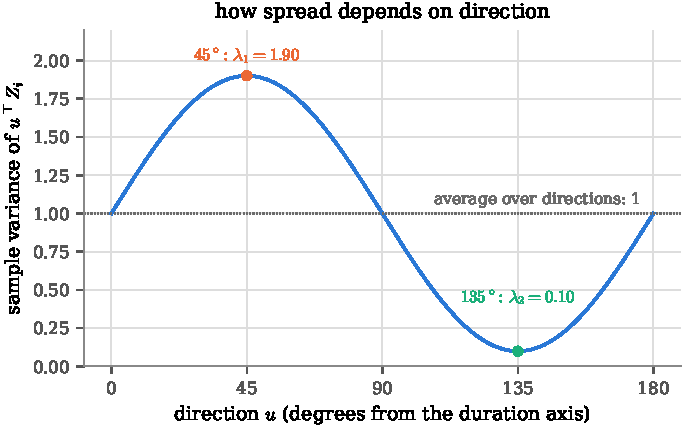
\includegraphics[width=0.78\textwidth]{fig_pca_direction}
\caption{The sample variance of $u^\top Z_i$ for the standardized Old Faithful data against the angle of the unit vector $u$: $1 + 0.90\sin 2t$, with its maximum $1.90$ at $45^\circ$ and its minimum $0.10$ at $135^\circ$.}
\label{fig:pcadirection}
\end{figure}

\section{The principal directions}
\label{sec:pca-directions}

$S$ is symmetric, so the spectral theorem \toolkit{sec:math-eigen} writes it as
\[
S = PDP^\top = \sum_{j=1}^d \lambda_jv_jv_j^\top, \qquad \lambda_1 \geq \lambda_2 \geq \cdots \geq \lambda_d \geq 0,
\]
with $P = (v_1, \ldots, v_d)$ orthogonal, so the $v_j$ are orthonormal, and the eigenvalues non-negative because $S$ is positive semidefinite.
The theorem of this chapter says the eigenvectors are the directions the cloud spreads along and the eigenvalues are the spreads.

\begin{theorem}[Principal directions]
\label{thm:pca-directions}
Let $S = PDP^\top$ as above. Then:
\begin{enumerate}[nosep]
\item $v_1$ maximizes $u^\top Su$ over unit vectors $u$, and the maximum is $\lambda_1$;
\item for $j = 2, \ldots, d$, $v_j$ maximizes $u^\top Su$ over unit vectors perpendicular to $v_1, \ldots, v_{j-1}$, and the maximum is $\lambda_j$;
\item the sample covariance matrix of the rotated points $P^\top X_i$ is $D$: the coordinates along the $v_j$ have sample variances $\lambda_j$ and sample covariances $0$; and $\sum_j\lambda_j = \mathrm{tr}(S)$, the sum of the $d$ sample variances.
\end{enumerate}
\end{theorem}
\coreproof{In the eigenvector coordinates $c = P^\top u$, the quadratic form is $\sum_j\lambda_jc_j^2$ with $\sum_jc_j^2 = 1$: a weighted average of the eigenvalues, largest when all the weight sits on the largest one. Perpendicularity to the first $j - 1$ eigenvectors sets their coordinates to zero, and the same argument runs on the rest.}
\begin{proof}
For a unit vector $u$ put $c = P^\top u$, so $u = Pc$ and $\norm{c}^2 = c^\top P^\top Pc = \norm{u}^2 = 1$.
Then $u^\top Su = c^\top P^\top PDP^\top Pc = c^\top Dc = \sum_j\lambda_jc_j^2 \leq \lambda_1\sum_jc_j^2 = \lambda_1$, with equality when $c = e_1$, that is, $u = v_1$: this is (1).
If $u$ is perpendicular to $v_1, \ldots, v_{j-1}$ then $c_1 = \cdots = c_{j-1} = 0$, since $c_k = v_k^\top u$, so $u^\top Su = \sum_{k \geq j}\lambda_kc_k^2 \leq \lambda_j$, with equality at $u = v_j$: this is (2).
For (3), the rotated points have mean $P^\top\bar{X}$ and sample covariance $\frac1n\sum_iP^\top(X_i - \bar{X})(X_i - \bar{X})^\top P = P^\top SP = D$; and $\mathrm{tr}(S) = \mathrm{tr}(PDP^\top) = \mathrm{tr}(DP^\top P) = \mathrm{tr}(D)$.
\end{proof}

\begin{definition}[Principal directions and components]
\label{def:pca}
The eigenvectors $v_1, \ldots, v_d$ of $S$, ordered by decreasing eigenvalue, are the sample's \textbf{principal directions}; the numbers $v_j^\top(X_i - \bar{X})$, $i = 1, \ldots, n$, are its $j$th \textbf{principal component} (or \textbf{scores}); and $\lambda_j/\mathrm{tr}(S)$ is the \textbf{proportion of the variance explained} by the $j$th component.
\end{definition}

\begin{inwords}
Rotate the axes so that the first points along the cloud's longest extent, the second along the longest extent perpendicular to it, and so on. In the new axes the coordinates are uncorrelated, their variances are the eigenvalues, and the total variance is the same as before, since a rotation does not change distances. The scores are the coordinates of each point in the new axes, measured from the center.

\textbf{For the kiss data.} With one variable there is one direction and nothing to rotate. For the standardized Old Faithful data (\cref{fig:pcacloud}), $v_1 = (0.71, 0.71)$ and $v_2 = (-0.71, 0.71)$ with $\lambda_1 = 1.90$ and $\lambda_2 = 0.10$: the first component is $(z_{i1} + z_{i2})/\sqrt2$, an eruption's size on the two measures combined, and carries $1.90/2 = 95\%$ of the variance; the second is $(z_{i2} - z_{i1})/\sqrt2$, how far the standardized wait sits above the standardized duration, and carries $5\%$.
\end{inwords}

\begin{figure}[htbp]
\centering
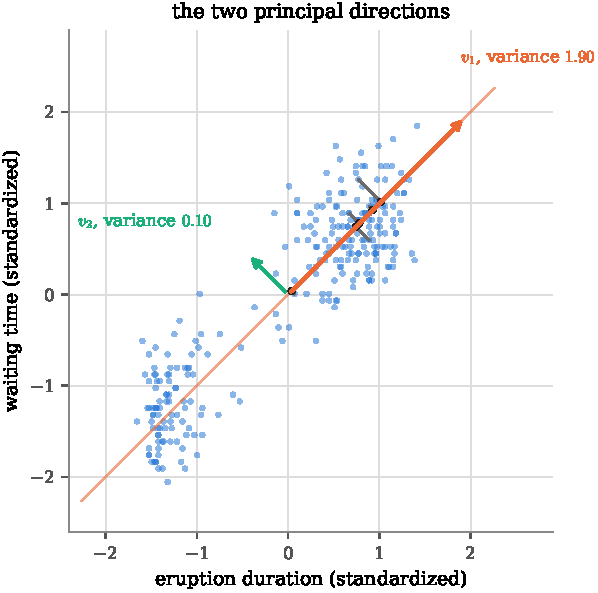
\includegraphics[width=0.6\textwidth]{fig_pca_cloud}
\caption{The standardized Old Faithful cloud with the line along its first principal direction, the two principal directions from the mean, each drawn with length $2\sqrt{\lambda_j}$, and five points of the upper cluster projected onto the first (gray segments, black dots).}
\label{fig:pcacloud}
\end{figure}

A correlation matrix with $1$s on the diagonal and $r$ off it always has eigenvectors $(1, 1)/\sqrt2$ and $(-1, 1)/\sqrt2$ with eigenvalues $1 + r$ and $1 - r$ (\cref{ex:pca-twobytwo}), so for two standardized variables the principal directions are the two diagonals whatever the data, the rising one first when $r > 0$, and only the eigenvalues carry information.
With more variables the directions are no longer fixed in advance, and they are what the method is for.
The method is Pearson's (1901), who found the line and the plane of closest fit to a cloud of points, which is \cref{thm:pca-projection} below; Hotelling (1933) named the principal components and tied them to the eigenvectors of the covariance matrix.

\begin{pitfall}[units decide the directions]
$u^\top Su$ is a variance, in the units of $u^\top X$, and changing the unit of one coordinate changes the eigenvectors, not just the eigenvalues. \Cref{fig:pcaunits} shows Old Faithful in its raw units, duration in minutes with variance $1.30$ and waiting in minutes with variance $184$: the first principal direction is tilted $86^\circ$ toward the waiting axis and explains $99.9\%$ of the variance, which says only that $184$ is much larger than $1.30$. Measure the duration in seconds instead and the picture tilts the other way. When the coordinates are measured in different units, or in the same unit on very different scales, standardize them first; the analysis is then of the correlation matrix, and the first direction is the one along which the standardized variables move together most. When the coordinates share a unit and their scales mean something, as with $d$ measurements of the same kind, the raw covariance matrix is the right object.
\end{pitfall}

\begin{figure}[htbp]
\centering
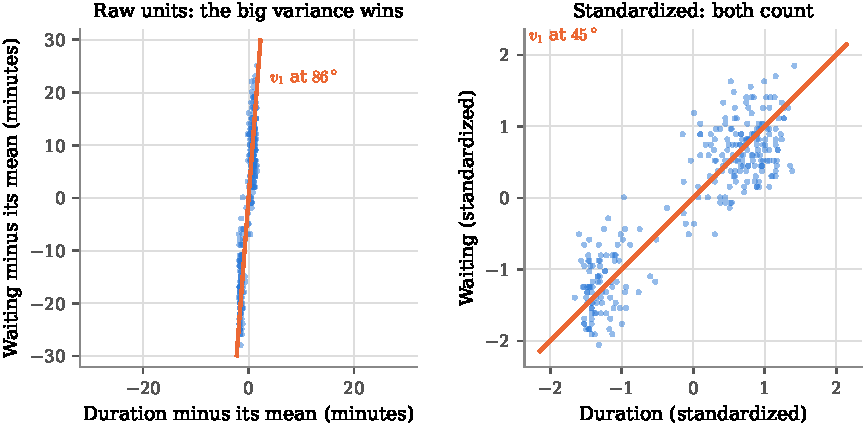
\includegraphics[width=\textwidth]{fig_pca_units}
\caption{Old Faithful with both axes in minutes (left, equal scales) and standardized (right). The first principal direction (orange) follows the variable with the larger variance on the left and the diagonal on the right.}
\label{fig:pcaunits}
\end{figure}

\section{The best flat picture}
\label{sec:pca-projection}

A cloud in $\real^d$ with $d > 3$ cannot be drawn.
Principal component analysis draws it anyway, by projecting it onto the plane (or the line, or a $k$-dimensional subspace) along which it is most spread out, and the point of the next theorem is that the plane which keeps the most variance is also the plane which loses the least distance.

\begin{theorem}[Projection onto the first $k$ principal directions]
\label{thm:pca-projection}
Let $S = PDP^\top$ as above, let $1 \leq k < d$, and for an orthonormal $u_1, \ldots, u_k$ let $Q$ be the projection onto their span, $Qx = \sum_{j \leq k}(u_j^\top x)u_j$.
Over all such choices, the sum of squared distances from the centered points to their projections,
\[
\sum_{i=1}^n\norm{(X_i - \bar{X}) - Q(X_i - \bar{X})}^2 = n\Big(\mathrm{tr}(S) - \sum_{j=1}^k u_j^\top Su_j\Big),
\]
is smallest when $u_1, \ldots, u_k$ span the same subspace as $v_1, \ldots, v_k$, and its minimum is $n(\lambda_{k+1} + \cdots + \lambda_d)$.
The projected cloud then has total variance (the sum of its $k$ sample variances) $\lambda_1 + \cdots + \lambda_k$, a proportion $(\lambda_1 + \cdots + \lambda_k)/\mathrm{tr}(S)$ of $\mathrm{tr}(S)$, the cloud's total.
\end{theorem}
\coreproof{Pythagoras splits each centered point's squared length into the part along the subspace and the part lost; summing, the lost part is the total variance minus the variance kept, $\sum_{j \leq k}u_j^\top Su_j$. Keeping the most is choosing $k$ orthonormal directions whose quadratic forms add up to the most, and in eigenvector coordinates that sum is $\sum_j\lambda_jw_j$ with weights $w_j \in [0, 1]$ adding up to $k$, which is largest with the weight on the $k$ largest eigenvalues.}
\begin{proof}
Write $Y_i = X_i - \bar{X}$.
Since $Q$ is an orthogonal projection, $\norm{Y_i}^2 = \norm{QY_i}^2 + \norm{Y_i - QY_i}^2$ \toolkit{sec:math-matrices}, and $\norm{QY_i}^2 = \sum_{j \leq k}(u_j^\top Y_i)^2$ by orthonormality.
Summing over $i$ and dividing by $n$, $\frac1n\sum_i\norm{Y_i}^2 = \mathrm{tr}(S)$ (the sum of the $d$ sample variances) and $\frac1n\sum_i(u_j^\top Y_i)^2 = u_j^\top Su_j$ (\cref{prop:pca-direction}, the $u_j^\top Y_i$ having mean $0$), which gives the displayed identity.
It remains to maximize $\sum_{j \leq k}u_j^\top Su_j$.
Put $c_j = P^\top u_j$, orthonormal since $P$ is orthogonal, so that $u_j^\top Su_j = \sum_m\lambda_mc_{jm}^2$ and
\[
\sum_{j=1}^k u_j^\top Su_j = \sum_{m=1}^d\lambda_mw_m, \qquad w_m = \sum_{j=1}^k c_{jm}^2.
\]
Each $w_m \leq 1$, since $c_{1m}, \ldots, c_{km}$ are the $m$th coordinates of $k$ orthonormal vectors, which extend to an orthonormal basis of $\real^d$, whose $m$th coordinates have squares summing to $1$ \toolkit{sec:math-gaussvec}; and $\sum_mw_m = \sum_j\norm{c_j}^2 = k$.
A sum $\sum_m\lambda_mw_m$ with $\lambda_1 \geq \cdots \geq \lambda_d$, $0 \leq w_m \leq 1$ and $\sum_mw_m = k$ is at most $\lambda_1 + \cdots + \lambda_k$: moving weight from any $m > k$ to any $m' \leq k$ with $w_{m'} < 1$ cannot decrease it, and when no such move is left the weights are $1$ on $m \leq k$ and $0$ after.
The bound is attained by $u_j = v_j$, where $c_j = e_j$; and any orthonormal $u_1, \ldots, u_k$ spanning the same subspace give the same projection $Q$, hence the same loss.
\end{proof}

\begin{inwords}
Among all flat pictures of dimension $k$, the one drawn on the first $k$ principal directions is the one in which the points move least from where they were, and what it loses is exactly the sum of the eigenvalues it leaves out. The proportion of the variance explained says how much of the cloud's variance the picture keeps.

\textbf{For the kiss data.} With $d = 1$ there is nothing to project. The standardized Old Faithful cloud projected onto $v_1$ (\cref{fig:pcacloud}) keeps $95\%$ of its variance, and the squared distances the points move add up to $n\lambda_2 = 272 \times 0.10 = 27$.
\end{inwords}

In practice the analysis runs in three steps: center the data (and standardize them unless the units agree), compute the eigenvectors and eigenvalues of $S$, and choose $k$.
The choice of $k$ is a judgment with two common guides.
The \textbf{scree plot} draws $\lambda_j$ against $j$ and stops where the fall flattens, the eigenvalues past that point being read as noise; the \textbf{proportion explained} chooses the smallest $k$ with $(\lambda_1 + \cdots + \lambda_k)/\mathrm{tr}(S)$ above a threshold such as $0.9$.
For a picture, $k$ is $2$ or $3$ whatever the eigenvalues say.

\begin{worked}[the stack loss data in four dimensions]
The $21$ days of \cref{ch:regression-multi} have four measurements each, air flow, water temperature, acid concentration and stack loss, in different units, so the analysis is of the correlation matrix, whose off-diagonal entries are $0.78$ (air, water), $0.50$ (air, acid), $0.92$ (air, loss), $0.39$ (water, acid), $0.88$ (water, loss) and $0.40$ (acid, loss). Its eigenvalues are $3.00$, $0.73$, $0.22$ and $0.05$, which explain $75\%$, $18\%$, $5\%$ and $1\%$ of the variance (\cref{fig:pcascree}): two components keep $93\%$. The first direction is $v_1 = (0.55, 0.52, 0.35, 0.55)$, close to an equal-weight average of the four standardized variables, an overall `how hard the plant was running' score, on which days $1$ to $3$ sit far to the right and days $17$ to $19$ far to the left. The second, $v_2 = (-0.08, -0.26, 0.93, -0.26)$, is the acid concentration against everything else: acid is the variable least tied to the other three (its correlations are $0.39$ to $0.50$), and the second component separates days by it, day $14$ at the top and day $17$ at the bottom. The regression of \cref{ch:regression-multi} explained the loss by the other three; the first component says the three and the loss mostly rise and fall together.
\end{worked}

\begin{figure}[htbp]
\centering
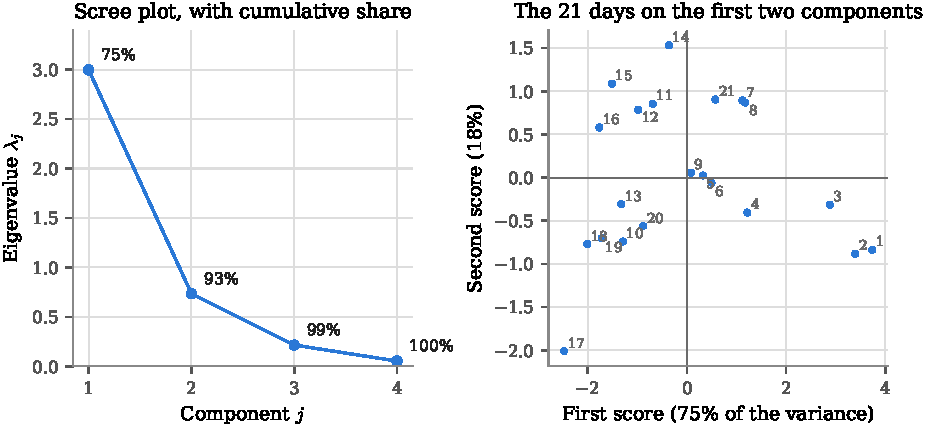
\includegraphics[width=\textwidth]{fig_pca_scree}
\caption{Stack loss, four standardized variables. Left: the scree plot of the eigenvalues $3.00$, $0.73$, $0.22$, $0.05$ with the cumulative share explained. Right: the $21$ days on their first two principal components, numbered.}
\label{fig:pcascree}
\end{figure}

\section{What the sample directions estimate}
\label{sec:pca-estimation}

Everything so far was a description of $n$ points, with no model behind it, and principal component analysis is used in that spirit on clouds that are not random at all.
When the $X_i$ are i.i.d.\ copies of a random vector $X$, the sample quantities estimate population ones, and the book's limit theorems say in what sense.

\begin{theorem}[Consistency of the sample covariance and its eigenvectors]
\label{thm:pca-consistent}
Let $X_1, X_2, \ldots$ be i.i.d.\ copies of $X \in \real^d$ with $\E[\norm{X}^4] < \infty$, mean $m$ and covariance matrix $\Sigma$, with eigenvalues $\lambda_1^* \geq \cdots \geq \lambda_d^*$ and orthonormal eigenvectors $v_1^*, \ldots, v_d^*$.
Then:
\begin{enumerate}[nosep]
\item $\bar{X} \convp m$ and $S \convp \Sigma$, entry by entry;
\item each sample eigenvalue converges: $\lambda_j \convp \lambda_j^*$ for $j = 1, \ldots, d$;
\item if $\lambda_j^*$ differs from both its neighbors, $\lambda_{j-1}^* > \lambda_j^* > \lambda_{j+1}^*$ (only the second inequality when $j = 1$, only the first when $j = d$), the sample direction converges to the population direction: with the signs chosen so that $v_j^\top v_j^* \geq 0$, $v_j \convp v_j^*$.
\end{enumerate}
\end{theorem}
\coreproof{Each entry of $S$ is an average of products of coordinates minus a product of averages, so the Law of Large Numbers and the continuous mapping theorem give (1); the eigenvalues, and the eigenvector lines where the eigenvalue is isolated, are continuous functions of the matrix, so the continuous mapping theorem gives (2) and (3).}
\recall{The Law of Large Numbers (\cref{thm:wlln}): for i.i.d.\ $Z_i$ with $\var(Z_i) < \infty$, $\frac1n\sum_iZ_i \convp \E[Z_i]$. The continuous mapping theorem (\cref{thm:cmt}): if $Y_n \convp y$ and $f$ is continuous, then $f(Y_n) \convp f(y)$; it holds for a vector $Y_n \convp y$ and a continuous $f$ of several variables, since continuity of $f$ at $y$ gives a $\delta$ with $\norm{f(z) - f(y)} \leq \epsilon$ whenever $\norm{z - y} \leq \delta$, so $\Pr(\norm{f(Y_n) - f(y)} > \epsilon) \leq \Pr(\norm{Y_n - y} > \delta) \to 0$; and a vector converges in probability as soon as each of its $q$ coordinates does, since $\Pr(\norm{Y_n - y} > \epsilon) \leq \sum_{j=1}^q\Pr(\abs{Y_n^{(j)} - y_j} > \epsilon/\sqrt{q})$.}
\begin{proof}
Write $S = \frac1n\sum_iX_iX_i^\top - \bar{X}\bar{X}^\top$ (expand the square in \cref{def:covmatrix}).
The $(j, k)$ entry of the first term is the average of the i.i.d.\ products $X_i^{(j)}X_i^{(k)}$, whose variance is finite by the fourth-moment assumption, so it converges in probability to $\E[X^{(j)}X^{(k)}]$; and $\bar{X}^{(j)} \convp m_j$ by the Law of Large Numbers with the second moments finite.
Since the vector of all $d + d^2$ quantities then converges in probability (each coordinate does), and $(a, b) \mapsto a - bb^\top$ is continuous, the continuous mapping theorem gives $S \convp \E[XX^\top] - mm^\top = \Sigma$ entry by entry, which is (1).
The map from a symmetric matrix to its $j$th largest eigenvalue is continuous \toolkit{sec:math-eigen}, so (2) follows from (1) by the continuous mapping theorem; and where $\lambda_j^*$ is isolated from its neighbors, the map to the unit eigenvector with the sign fixed by $v_j^\top v_j^* \geq 0$ is continuous at $\Sigma$, which gives (3) (the map need only be continuous where the limit lives, as \cref{ch:limit-tools} notes).
\end{proof}

The condition in (3) is not decoration: when two population eigenvalues are equal, any direction in the plane they span is an eigenvector, and the sample direction wanders in that plane however large $n$ is.
For the standardized Old Faithful data, the gap $1.90$ against $0.10$ is wide, and the sample directions are the population's diagonals in any case.
There is a Central Limit Theorem to go with the Law: for Gaussian data, $\sqrt{n}(\lambda_j - \lambda_j^*) \convd \Gauss(0, 2\lambda_j^{*2})$ when $\lambda_j^*$ is isolated (Anderson, 1963), so a sample eigenvalue has a standard error of about $\lambda_j\sqrt{2/n}$; it is stated here and not proved, and nothing depends on it.

\begin{pitfall}[many variables, few observations]
The theorem lets $n$ grow with $d$ fixed. When $d$ is comparable to $n$, or larger, $S$ is a poor estimate of $\Sigma$ even though each of its entries is consistent: with $d > n$ the cloud spans at most $n - 1$ dimensions, $S$ has rank at most $n - 1$, and at least $d - n + 1$ of its eigenvalues are exactly $0$ whatever $\Sigma$ is. The largest sample eigenvalue is then biased upward and the smallest downward, and the first sample direction can be far from $v_1^*$ even when the gap below $\lambda_1^*$ is wide. Gene expression data, with thousands of genes measured on hundreds of people, are the standard case. The remedies assume something about $\Sigma$: that it has low rank, so that only the first $k$ sample components are kept and the rest treated as noise, or that $v_1^*$ has few nonzero coordinates (sparse principal components), both outside this book.
\end{pitfall}

\section{Where the book ends}
\label{sec:pca-end}

The book began with $124$ couples and one proportion, and it ends with $21$ days and a four-by-four matrix, but the tools did not change.
A model says what the data could have been; an estimator is a function of the data; the Law of Large Numbers says it settles down, the Central Limit Theorem says how, and Slutsky, the continuous mapping theorem and the delta method carry those two facts to every estimator built from averages, which is nearly all of them.
Maximum likelihood turned those tools into a method, with the Fisher information as its yardstick; tests and intervals were the same calculation read two ways; the Bayesian chapters put a prior on the parameter and found, in large samples, the same answers; regression and its generalizations put a linear predictor behind the mean; and this chapter dropped the response and kept the covariance.
What comes after, in the next book of the series, is the same tools, the theorems of \cref{ch:lln,ch:clt,ch:limit-tools}, applied to harder models.

\section{Summary}
\label{sec:pca-summary}

\begin{itemize}[nosep]
\item A sample of vectors is a cloud in $\real^d$ with mean vector $\bar{X}$ and sample covariance matrix $S = \frac1n\sum_i(X_i - \bar{X})(X_i - \bar{X})^\top$; $u^\top Su$ is the cloud's variance along $u$. Old Faithful: variances $1.30$ and $184$, covariance $13.9$, correlation $0.90$.
\item Spectral theorem: $S = PDP^\top$ with orthonormal eigenvectors and eigenvalues $\lambda_1 \geq \cdots \geq \lambda_d \geq 0$. The eigenvectors are the principal directions: $v_1$ maximizes $u^\top Su$ with value $\lambda_1$, $v_j$ does so among directions perpendicular to the earlier ones, the rotated coordinates are uncorrelated with variances $\lambda_j$, and $\sum_j\lambda_j = \mathrm{tr}(S)$.
\item Projecting onto the first $k$ principal directions loses $n(\lambda_{k+1} + \cdots + \lambda_d)$ in squared distance, less than any other $k$-dimensional projection, and keeps the proportion $(\lambda_1 + \cdots + \lambda_k)/\mathrm{tr}(S)$ of the variance. Choose $k$ by the scree plot or a proportion threshold. Stack loss: $75\%$, $93\%$, $99\%$, with an overall-activity first direction and an acid-against-the-rest second.
\item Standardize when the units differ: in raw minutes Old Faithful's first direction is at $86^\circ$ and explains $99.9\%$, which only reports the ratio of two variances.
\item With i.i.d.\ data and fourth moments, $S \convp \Sigma$ entry by entry (LLN and CMT), the eigenvalues converge, and each eigenvector converges where its eigenvalue is isolated. For Gaussian data $\sqrt{n}(\lambda_j - \lambda_j^*) \convd \Gauss(0, 2\lambda_j^{*2})$ (stated). With $d$ near or above $n$ the sample eigenvalues are badly biased and extra assumptions are needed.
\end{itemize}

\section{Exercises}
\label{sec:pca-exercises}

\begin{exercise}
\label{ex:pca-twobytwo}
(a) Show that $\begin{pmatrix} 1 & r \\ r & 1\end{pmatrix}$ has eigenvectors $(1, 1)/\sqrt2$ and $(-1, 1)/\sqrt2$ with eigenvalues $1 + r$ and $1 - r$, and check the Old Faithful values $1.90$ and $0.10$. (b) Show that for the unit vector $u = (\cos t, \sin t)$, $u^\top Su = 1 + r\sin 2t$, the curve of \cref{fig:pcadirection}, and find its average over $t$. (c) For a general $2 \times 2$ covariance matrix $\begin{pmatrix} a & c \\ c & b\end{pmatrix}$, show that the first principal direction makes the angle $\frac12\arctan\big(2c/(a - b)\big)$ with the first axis (when $a > b$; when $a < b$ the maximum is at the other root of $\tan 2t = 2c/(a - b)$, $90^\circ$ away), and compute it for Old Faithful's raw $S$.
\end{exercise}
\begin{solution}
(a) $\begin{pmatrix} 1 & r \\ r & 1\end{pmatrix}\begin{pmatrix} 1 \\ 1\end{pmatrix} = (1 + r)\begin{pmatrix} 1 \\ 1\end{pmatrix}$ and likewise $(1 - r)$ for $(-1, 1)$; with $r = 0.90$, $1.90$ and $0.10$. (b) $u^\top Su = \cos^2t + \sin^2t + 2r\sin t\cos t = 1 + r\sin 2t$; its average over a full turn is $1$, the average of the eigenvalues, that is, $\mathrm{tr}(S)/d$. (c) $u^\top Su = a\cos^2t + b\sin^2t + 2c\sin t\cos t = \frac{a + b}{2} + \frac{a - b}{2}\cos 2t + c\sin 2t$, whose derivative in $t$ vanishes when $\tan 2t = 2c/(a - b)$. For Old Faithful $a < b$, and $2 \times 13.9/(1.30 - 184.1) = -0.152$ gives $2t = -8.6^\circ$ for the minimum and $2t = 180^\circ - 8.6^\circ$ for the maximum, so $t = 85.7^\circ$, the $86^\circ$ of \cref{fig:pcaunits}.
\end{solution}

\begin{exercise}
\label{ex:pca-projector}
Let $H = I - \frac1n\mathbf{1}\mathbf{1}^\top$ with $\mathbf{1} \in \real^n$ the vector of ones. Show that $H$ is symmetric with $H^2 = H$, say onto which subspace it projects, and verify $S = \frac1n\mathbf{X}^\top H\mathbf{X}$ for the $n \times d$ data matrix $\mathbf{X}$.
\end{exercise}
\begin{solution}
$H^\top = H$ is clear, and $H^2 = I - \frac2n\mathbf{1}\mathbf{1}^\top + \frac{1}{n^2}\mathbf{1}(\mathbf{1}^\top\mathbf{1})\mathbf{1}^\top = I - \frac1n\mathbf{1}\mathbf{1}^\top = H$ since $\mathbf{1}^\top\mathbf{1} = n$. $H\mathbf{1} = 0$ and $Hv = v$ for $v \perp \mathbf{1}$, so $H$ projects onto the vectors with coordinates summing to $0$, the orthogonal complement of the line through $\mathbf{1}$ (the residual projection of \cref{ch:regression-multi} for the intercept-only model). $H\mathbf{X}$ subtracts each column's mean from the column, so its rows are $(X_i - \bar{X})^\top$, and $\frac1n\mathbf{X}^\top H\mathbf{X} = \frac1n(H\mathbf{X})^\top(H\mathbf{X}) = \frac1n\sum_i(X_i - \bar{X})(X_i - \bar{X})^\top = S$, using $H^\top H = H$.
\end{solution}

\begin{exercise}
\label{ex:pca-scores}
Show that the principal components are uncorrelated: for $j \neq k$ the sample covariance of the scores $v_j^\top(X_i - \bar{X})$ and $v_k^\top(X_i - \bar{X})$ is $v_j^\top Sv_k = 0$. Then show that the $n \times d$ matrix of scores is $H\mathbf{X}P$ and that its columns have squared lengths $n\lambda_j$.
\end{exercise}
\begin{solution}
The scores have mean $0$, so their sample covariance is $\frac1n\sum_iv_j^\top(X_i - \bar{X})(X_i - \bar{X})^\top v_k = v_j^\top Sv_k = v_j^\top\lambda_kv_k = 0$ by orthonormality. The score matrix has $(i, j)$ entry $(X_i - \bar{X})^\top v_j$, which is the $(i, j)$ entry of $H\mathbf{X}P$; the $j$th column's squared length is $\sum_i(v_j^\top(X_i - \bar{X}))^2 = nv_j^\top Sv_j = n\lambda_j$.
\end{solution}

\begin{exercise}
\label{ex:pca-reconstruct}
With $P_k = (v_1, \ldots, v_k)$, the reconstruction of $X_i$ from its first $k$ scores is $\hat{X}_i = \bar{X} + P_kP_k^\top(X_i - \bar{X})$. (a) Show that $\frac1n\sum_i\norm{X_i - \hat{X}_i}^2 = \lambda_{k+1} + \cdots + \lambda_d$. (b) For the stack loss data, what fraction of the standardized cloud's squared size does a two-component reconstruction lose, and how many days' worth of squared distance is that?
\end{exercise}
\begin{solution}
(a) $P_kP_k^\top$ is the projection onto the span of $v_1, \ldots, v_k$, so by \cref{thm:pca-projection} with $u_j = v_j$ the sum of squared distances is $n(\lambda_{k+1} + \cdots + \lambda_d)$. (b) $(0.215 + 0.053)/4 = 6.7\%$; the squared distances lost add up to $21 \times 0.268 = 5.6$, against a total squared size $21 \times 4 = 84$.
\end{solution}

\begin{exercise}
\label{ex:pca-gaussian}
Let $X \sim \Gauss_d(m, \Sigma)$ with $\Sigma = PDP^\top$ positive definite. (a) Show that the population components $v_j^{*\top}(X - m)$ are independent $\Gauss(0, \lambda_j^*)$. (b) Show that the contours of the density of $X$ are the ellipsoids $(x - m)^\top\Sigma^{-1}(x - m) = c$, whose axes are the eigenvectors with half-lengths proportional to $\sqrt{\lambda_j^*}$: the principal directions are the axes of the Gaussian's ellipse, as in the confidence ellipse of \cref{ch:regression-multi}.
\end{exercise}
\begin{solution}
(a) $P^\top(X - m)$ is Gaussian with mean $0$ and covariance $P^\top\Sigma P = D$ \toolkit{sec:math-gaussvec}; a Gaussian vector with diagonal covariance has independent coordinates, with variances the diagonal entries. (b) The density is proportional to $\exp(-\frac12(x - m)^\top\Sigma^{-1}(x - m))$, and $\Sigma^{-1} = PD^{-1}P^\top$, so with $z = P^\top(x - m)$ the exponent is $-\frac12\sum_jz_j^2/\lambda_j^*$: a level set $\sum_jz_j^2/\lambda_j^* = c$ is an ellipsoid in the eigenvector coordinates with semi-axes $\sqrt{c\lambda_j^*}$ along $v_j^*$.
\end{solution}

\begin{exercise}
\label{ex:pca-variance-of-S}
In \cref{thm:pca-consistent}, where exactly is the fourth-moment assumption used, and what would fail without it? Show by an example with $d = 1$ that $S$ can be consistent for $\Sigma$ when only $\E[X^2] < \infty$ holds, so that the assumption is a convenience of the proof rather than a necessity.
\end{exercise}
\begin{solution}
It makes $\var(X^{(j)}X^{(k)}) \leq \E[(X^{(j)})^2(X^{(k)})^2] \leq \E[\norm{X}^4] < \infty$, which is the finite-variance hypothesis of \cref{thm:wlln} for the averages $\frac1n\sum_iX_i^{(j)}X_i^{(k)}$; without it that theorem does not apply. With $d = 1$ and $\E[X^2] < \infty$, $\frac1n\sum_iX_i^2$ is an average of i.i.d.\ variables with finite mean, which the Strong Law (\cref{thm:slln}, needing only a finite mean; almost sure convergence implies convergence in probability, \cref{app:modes}) covers without a variance, so $\frac1n\sum_iX_i^2 \convp \E[X^2]$, $\bar{X} \convp m$, and $S = \frac1n\sum_iX_i^2 - \bar{X}^2 \convp \var(X)$ by the continuous mapping theorem; the same argument works entrywise for any $d$, since $\E\abs{X^{(j)}X^{(k)}} \leq \sqrt{\E[(X^{(j)})^2]\,\E[(X^{(k)})^2]} < \infty$ by the Cauchy--Schwarz inequality, so the fourth moment is only what the book's weak law asks for.
\end{solution}

\begin{exercise}
\label{ex:pca-equal}
Let $\Sigma = I_2$, so that every direction is a population eigenvector with eigenvalue $1$. Explain why the first sample principal direction has no limit as $n \to \infty$, even though $S \convp I_2$, and why this is consistent with \cref{thm:pca-consistent}. What does a scree plot look like in this case?
\end{exercise}
\begin{solution}
$S - I_2$ is a small symmetric matrix of random sign, and the first eigenvector of $S$ is the first eigenvector of $S - I_2$ (adding $I_2$ shifts every eigenvalue by $1$ and changes no eigenvector), whose direction depends on which way the random perturbation happens to point and does not settle down. The theorem's (3) requires $\lambda_1^* > \lambda_2^*$, which fails here; (1) and (2) hold, and both sample eigenvalues converge to $1$. The scree plot is nearly flat, two eigenvalues a little above and below $1$, which is the plot's way of saying there is no preferred direction.
\end{solution}

\begin{exercise}
\label{ex:pca-regression}
Principal components and regression. (a) Show that regressing the first score $v_1^\top(X_i - \bar{X})$ on the second by least squares through the origin gives slope $0$. (b) For the standardized Old Faithful data, the regression of waiting on duration has slope $r = 0.90$ (\cref{ch:regression-uni}), while the first principal direction is the $45^\circ$ line with slope $1$. Explain why the two lines differ, and which one minimizes which distance.
\end{exercise}
\begin{solution}
(a) The slope is the sample covariance of the two scores over the variance of the second, and the covariance is $0$ by \cref{ex:pca-scores}. (b) Least squares minimizes the sum of squared vertical distances, from each point to the line along the waiting axis, and gives the regression line of \cref{ch:regression-uni}, whose slope $r < 1$ is the regression toward the mean of that chapter; the first principal direction minimizes the sum of squared perpendicular distances (\cref{thm:pca-projection} with $k = 1$), and treats the two variables alike, which for standardized variables with positive correlation always gives the diagonal. The regression line is the right one for predicting waiting from duration; the principal direction is the right one for describing the cloud.
\end{solution}


\appendix
\part*{Appendices}
\addcontentsline{toc}{part}{Appendices}
\chapter{Mathematical Toolkit}
\label{app:math}

This appendix collects the mathematical habits the book uses: not statistics, but the handful of ideas from calculus, sets and probability that the proofs lean on.
Each entry says what the idea is in plain words, draws it, and names the first place in the book that needs it.
When a chapter marks a step with `(toolkit \ref{sec:math-mvt})', this is where to come.
Nothing here is needed to state a result; everything here is needed to follow a proof.
Later chapters will add entries of their own (vectors and matrices for regression, the chi-squared family for tests) at the end.

\section{Limits of sequences of numbers}
\label{sec:math-limits}

A sequence of numbers $x_1, x_2, x_3, \ldots$ \textbf{converges} to $x$ if the terms eventually stay as close to $x$ as you like.
The definition makes `as close as you like' and `eventually' precise:
\[
\text{for every } \epsilon > 0 \text{ there is an index } N \text{ such that } \abs{x_n - x} < \epsilon \text{ for all } n \geq N.
\]
Read it as a game with an opponent.
The opponent names a tolerance $\epsilon$, any positive number, however small.
You must answer with an index $N$ past which every term of the sequence is within $\epsilon$ of $x$.
If you can always answer, the sequence converges.
The order of the two moves is the whole content: $\epsilon$ is chosen first and $N$ is allowed to depend on it, which is why a smaller $\epsilon$ is usually met with a larger $N$ (\cref{fig:tk-epsilon}).
Writing the moves in the other order (`there is an $N$ that works for every $\epsilon$') would say the sequence is eventually \textit{equal} to $x$, a much stronger and usually false statement.
The left of \cref{fig:tk-epsilon} plays the game for $x_n = 2 + (-1)^n/\sqrt{n}$ with two tolerances: for $\epsilon = 0.3$ every term past $N = 12$ is inside the band, and for $\epsilon = 0.1$ you need $N = 101$ (at $n = 100$ the term sits exactly on the band's edge, and the definition asks for strictly inside).
The right draws the index that works as a function of the tolerance; it climbs as $\epsilon$ shrinks, and convergence means the staircase is defined for every $\epsilon > 0$, however small.

\begin{figure}[htbp]
\centering
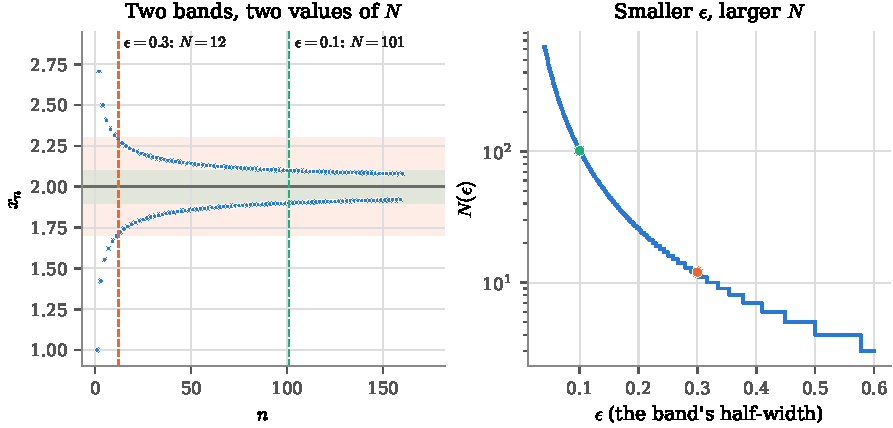
\includegraphics[width=\textwidth]{fig_tk_epsilon_n}
\caption{The $\epsilon$-$N$ definition as a game. Left: the sequence $x_n = 2 + (-1)^n/\sqrt{n}$ with the bands $2 \pm 0.3$ and $2 \pm 0.1$. Right: the smallest index $N$ that works, as a function of the tolerance $\epsilon$.}
\label{fig:tk-epsilon}
\end{figure}

\textbf{Where the book uses it.} \Cref{sec:conv-why} starts from this definition and explains why it cannot be applied directly to random variables; \cref{def:convp} keeps its shape but applies it to the \textit{probabilities} $\Pr(\abs{X_n - X} \geq \epsilon)$, which are ordinary numbers.
Every `$\to 0$' in a proof of convergence in probability is this definition applied to a sequence of numbers.

\textbf{Limits inside an expectation.} One further fact is used in the uniform law of large numbers of \cref{sec:proof-ulln} and, for an integral in place of an expectation, in \cref{ch:exp-families}: if random variables $W_r$ converge to $0$ as $r \to 0$ for every outcome, and all of them are bounded by one fixed random variable $G$ with $\E[G] < \infty$, then $\E[W_r] \to 0$ as well. This is the dominated convergence theorem. The bound is what makes it true: without it, a $W_r$ that is huge on a set of tiny probability can have an expectation that refuses to go to $0$ even though $W_r$ itself goes to $0$ at every outcome.

\section{Supremum and infimum}
\label{sec:math-sup}

The \textbf{maximum} of a set of numbers is its largest member.
Some sets have none: $\{1 - \frac{1}{n} : n = 1, 2, \ldots\}$ climbs toward $1$ and never reaches it.
The \textbf{supremum}, written $\sup$, is the least upper bound: the smallest number that no member exceeds.
For that set the supremum is $1$, which is not a member.
When a maximum exists it equals the supremum; the supremum exists more often, which is why proofs prefer it.
The \textbf{infimum}, $\inf$, is the greatest lower bound, and the same remarks apply with `minimum'.
\Cref{fig:tk-sup} shows both cases.
On the left, the set $\{1 - 1/n\}$ has no largest element, but $1$ is its least upper bound.
On the right, $x e^{-x}$ on $[0, 4]$ attains its supremum at $x = 1$ and its infimum at $x = 0$, so there $\sup = \max$ and $\inf = \min$; a continuous function on a closed, bounded interval always attains both. The same holds on any closed, bounded set in $\real^d$, such as a closed ball (the extreme value theorem).

\begin{figure}[htbp]
\centering
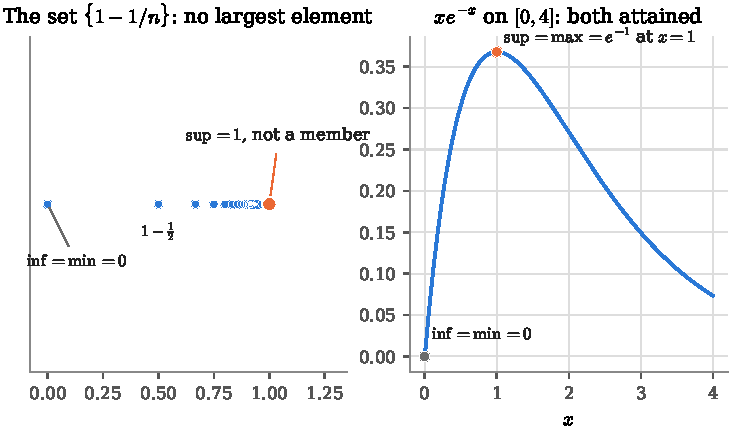
\includegraphics[width=\textwidth]{fig_tk_sup}
\caption{Left: the set $\{1 - 1/n : n = 1, 2, \ldots\}$ and its supremum $1$. Right: the function $x e^{-x}$ on $[0, 4]$.}
\label{fig:tk-sup}
\end{figure}

\textbf{Where the book uses it.} The conservative confidence interval of \cref{sec:ci-three-solutions} replaces $\sqrt{p(1-p)}$ by its supremum over $p \in (0,1)$, which is $\frac12$ and is attained; the subway version has $\sup_\lambda \lambda = \infty$, which is why no conservative interval exists there. \Cref{ch:estimators} mentions that a statistic may be defined through a $\sup$ or $\inf$; the maximum of a sample, $\max_i X_i$, is a maximum of finitely many numbers and causes no trouble. The proofs of consistency in \cref{thm:mle-consistent,thm:gof-family} use the extreme value theorem on a closed, bounded set of parameters.

\section{Sets, maps and one-to-one}
\label{sec:math-maps}

A \textbf{map} (or function) $f$ from a set $A$ to a set $B$ assigns to each element of $A$ exactly one element of $B$.
Its \textbf{image} is the set of elements of $B$ that are actually hit.
The map is \textbf{injective} (one-to-one) if different inputs always give different outputs: $a_1 \neq a_2$ implies $f(a_1) \neq f(a_2)$, or, turned around, $f(a_1) = f(a_2)$ implies $a_1 = a_2$.
An injective map can be undone: from the output you can recover the input.
For a function of one real variable the test is visual, the horizontal-line test of \cref{fig:tk-injective}: if some horizontal line crosses the graph twice, two inputs share an output and the map is not injective.
On the left of the figure, $\lambda \mapsto e^{-5\lambda}$ is strictly decreasing, so every height is hit once and $\lambda$ can be read off the output; this is the map of the censored-exponential example of \cref{ex:censored-expo}.
On the right, $x \mapsto x^2$ on $[-2, 2]$ hits the height $1$ twice, so the input cannot be recovered from the output.
A strictly increasing or strictly decreasing function always passes the test.

\begin{figure}[htbp]
\centering
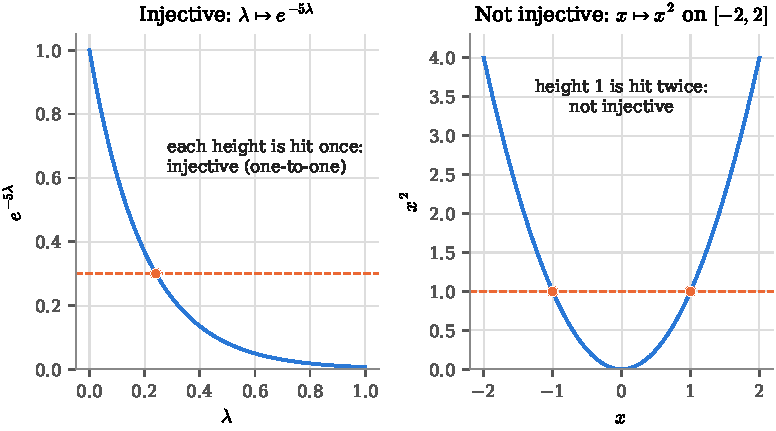
\includegraphics[width=\textwidth]{fig_tk_injective}
\caption{The horizontal-line test. Left: $\lambda \mapsto e^{-5\lambda}$, the map of the censored-exponential example of \cref{ex:censored-expo}. Right: $x \mapsto x^2$ on $[-2, 2]$.}
\label{fig:tk-injective}
\end{figure}

A \textbf{partition} of a set is a way of cutting it into pieces that do not overlap and together cover everything; any map partitions its domain into the sets of inputs that share an output.

\textbf{Where the book uses it.} Identifiability (\cref{def:identifiable}) is exactly the statement that the map $\theta \mapsto \Pr_\theta$ is injective; every identifiability argument in \cref{ch:models} is a horizontal-line test on that map. A statistic partitions the sample space (\cref{sec:est-reduction}).

\section{Indicator functions}
\label{sec:math-indicator}

The \textbf{indicator} of an event or a condition is the function that is $1$ when the condition holds and $0$ when it does not: $\ind(x \geq 5)$ is $0$ for $x < 5$ and $1$ from $5$ on.
It is the simplest random variable there is, a coin that comes up $1$ with probability $\Pr(\text{condition})$, and its expectation is that probability:
\[
\E[\ind(X \geq 5)] = 1 \cdot \Pr(X \geq 5) + 0 \cdot \Pr(X < 5) = \Pr(X \geq 5).
\]
That one line, \textit{the expectation of an indicator is a probability}, is how probabilities enter computations that are written with expectations, and how a sum of indicators becomes a count (the number of couples turning right is $\sum_i \ind(R_i = 1)$).
\Cref{fig:tk-indicator} draws the two sides of the line: on the left the indicator $\ind(x \geq 5)$, a step from $0$ to $1$; on the right, for $X \sim \Expo(0.16)$, its expectation as the shaded probability $\Pr(X \geq 5) = e^{-5 \times 0.16} = 0.45$.

\begin{figure}[htbp]
\centering
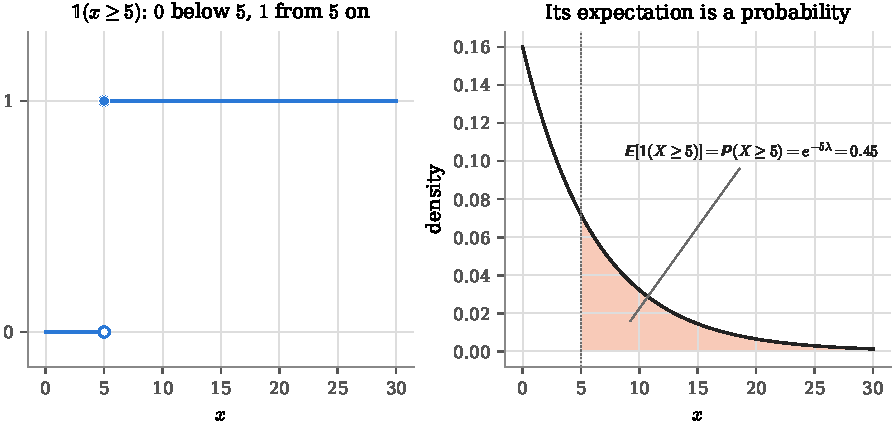
\includegraphics[width=\textwidth]{fig_tk_indicator}
\caption{Left: the indicator $\ind(x \geq 5)$ as a function of $x$. Right: the density of $X \sim \Expo(0.16)$, with the probability $\Pr(X \geq 5)$ shaded.}
\label{fig:tk-indicator}
\end{figure}

\textbf{Where the book uses it.} The CDF of a constant is a step function (\cref{ex:unif-shrinking}); the censored observations of \cref{ch:models} are indicators of the unobserved variable; the Strong Law in \cref{app:modes} counts failures with a sum of indicators; Markov's inequality below is proved with one.

\section{Random variables as functions, and `almost surely'}
\label{sec:math-rv}

A \textbf{random variable} is a function from the sample space (the set of possible outcomes of an experiment) to the real line.
\Cref{fig:tk-rv} draws the simplest case: the $36$ outcomes of two dice, and the function $X = $ `the sum'.
The probability $\Pr(X = 7)$ is the probability of the set of outcomes that $X$ sends to $7$: six of the $36$, so $\Pr(X = 7) = 6/36$ on the right of the figure.
Two random variables on the same sample space, say the sum $X$ and the larger die $Y$, are two functions of the \textit{same} outcome, which is what gives meaning to $X - Y$ and to `$X$ and $Y$ are close': you compare them outcome by outcome.
This is the viewpoint \cref{sec:conv-why} needs for a sequence of random variables, which is a sequence of functions on one sample space.

\begin{figure}[htbp]
\centering
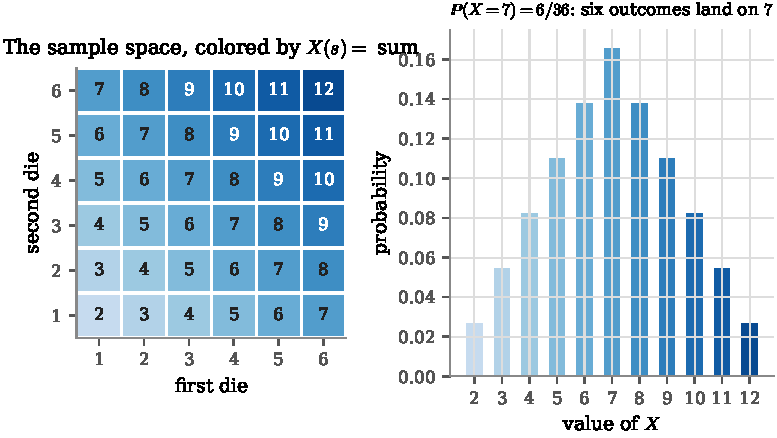
\includegraphics[width=\textwidth]{fig_tk_rv_function}
\caption{A random variable as a function on the sample space. Left: the $36$ outcomes of two dice, each colored by the value the function $X = $ `sum' assigns it. Right: the distribution of $X$ on the real line.}
\label{fig:tk-rv}
\end{figure}

Three phrases from probability theory appear in the book and mean less than they sound.
\begin{itemize}[nosep]
\item \textbf{Almost surely} means `with probability one'. A continuous random variable equals any particular number with probability zero, so `$X \neq 5$ almost surely' is true even though the outcome $X = 5$ is not impossible; the set of outcomes where a statement fails is allowed to be nonempty as long as it has probability zero. The book uses it in Hoeffding's inequality (`bounded almost surely': the probability of landing outside $[a, b]$ is zero) and in \cref{app:modes}.
\item \textbf{Measurable} (a measurable function, a measurable sample space) is the technical condition that makes probabilities of the relevant events well defined. Every function you can write down with formulas, limits, sums and integrals is measurable; the usual rule of thumb, that anything you can compute from the data is a statistic, is correct in practice. The book never needs more.
\item A \textbf{probability measure} (or distribution) assigns a probability to every event. A PMF or PDF is a recipe for one: sum or integrate it over the event. The two determine each other, and the book writes down families of distributions through their PMFs and PDFs (\cref{def:statmodel}).
\end{itemize}

\section{Densities, CDFs and quantiles}
\label{sec:math-density}

For a continuous random variable, \textbf{probability is area}: $\Pr(a \leq X \leq b)$ is the area under the density $f$ between $a$ and $b$.
The \textbf{CDF} $F(x) = \Pr(X \leq x)$ is the area accumulated up to $x$, so $\Pr(a \leq X \leq b) = F(b) - F(a)$, and $F$ is the antiderivative of $f$: $f = F'$.
The \textbf{quantile} reads the CDF backwards: given a probability $u$, the quantile is the $x$ with $F(x) = u$; the book's $q_\alpha$ is the case $u = 1 - \alpha$, indexed by the probability \textit{above} the cutoff.
\Cref{fig:tk-density} draws the three on one example, the standard Gaussian.
At the top, the shaded area under the density between $a = -1$ and $b = 1$ is $\Pr(a \leq X \leq b) = 0.683$.
At the bottom, the same probability is the rise of the CDF from $F(a)$ to $F(b)$, and reading the CDF sideways at $0.95$ gives the quantile $q_{0.05} = 1.645$ of \cref{sec:gauss-quantiles}.
The same three ideas work for a discrete random variable with sums in place of integrals: the PMF is the list of probabilities, the CDF the running total, and the CDF jumps at each possible value instead of rising smoothly.

\begin{figure}[htbp]
\centering
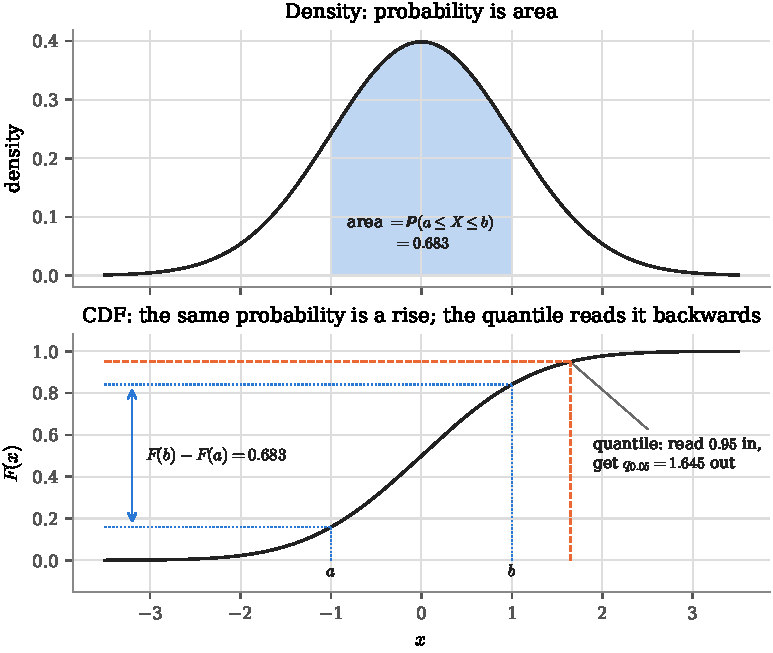
\includegraphics[width=0.78\textwidth]{fig_tk_density_cdf}
\caption{Density, CDF and quantile for $\Gauss(0,1)$. Top: the density, with the area between $a = -1$ and $b = 1$ shaded. Bottom: the CDF, with the rise from $F(a)$ to $F(b)$ and the quantile $q_{0.05}$ marked.}
\label{fig:tk-density}
\end{figure}

\textbf{Where the book uses it.} Convergence in distribution (\cref{def:convd}) compares CDFs, and the jumps of a discrete CDF are why only continuity points count. Every probability in \cref{ch:gaussian} is a CDF lookup. The density of a transformed variable, such as $aX + b$ or $X^2$, is found by writing its CDF and differentiating (\cref{sec:gauss-properties}, \cref{ch:models}).

\section{Three inequalities}
\label{sec:math-inequalities}

\textbf{The triangle inequality:} $\abs{x + y} \leq \abs{x} + \abs{y}$, and so $\abs{x - z} \leq \abs{x - y} + \abs{y - z}$: a detour through $y$ is never shorter than the direct distance.
Proofs use it to split an error into two pieces, for instance $\abs{T_n - \mu} \leq \abs{T_n - \E[T_n]} + \abs{\E[T_n] - \mu}$ in \cref{prop:shrinking-variance}: if the total is at least $\epsilon$, one of the two pieces is at least $\epsilon/2$.

\textbf{Markov's inequality:} if $Y \geq 0$ then $\Pr(Y \geq a) \leq \E[Y]/a$ for every $a > 0$.
The picture (\cref{fig:tk-inequalities}, left) is the proof: the step function $a \cdot \ind(Y \geq a)$ never exceeds $Y$, so its expectation, $a \Pr(Y \geq a)$, is at most $\E[Y]$.
A non-negative variable with a small mean is rarely large.

\textbf{Chebyshev's inequality:} for any random variable with finite variance, $\Pr(\abs{T - \E[T]} \geq \epsilon) \leq \var(T)/\epsilon^2$.
It is Markov's inequality applied to $Y = (T - \E[T])^2$ with $a = \epsilon^2$.
In standard-deviation units it says $\Pr(\abs{T - \E[T]} \geq k \sigma) \leq 1/k^2$ for every distribution whatsoever, which is both its strength (universal) and its weakness (loose: for a Gaussian the true two-standard-deviation tail is $0.046$, the bound says $0.25$).
The right of \cref{fig:tk-inequalities} draws the bound $1/k^2$ against the exact tail probabilities of a Gaussian and of an $\Expo(1)$ variable: the bound holds for every distribution and is far from tight for these two.

\begin{figure}[htbp]
\centering
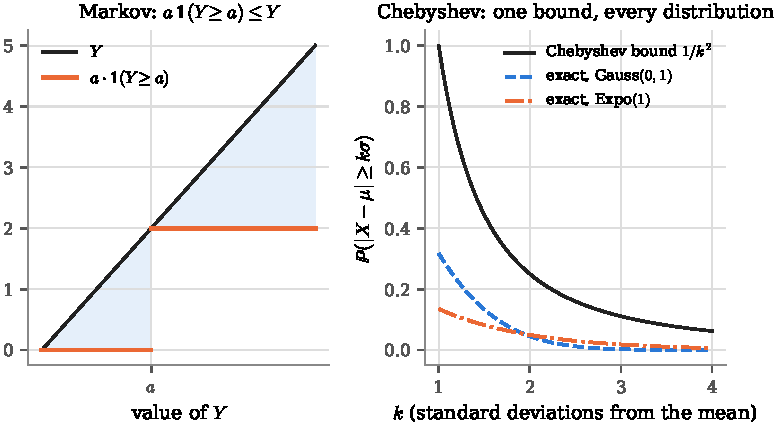
\includegraphics[width=\textwidth]{fig_tk_inequalities}
\caption{Left: $Y$ and the step function $a \cdot \ind(Y \geq a)$. Right: Chebyshev's bound $1/k^2$ against the exact probabilities $\Pr(\abs{T - \E[T]} \geq k\sigma)$ for a Gaussian $T$ and for $T \sim \Expo(1)$.}
\label{fig:tk-inequalities}
\end{figure}

\textbf{Where the book uses it.} The Law of Large Numbers (\cref{thm:wlln}) is Chebyshev's inequality with $n \to \infty$; the shrinking-variance criterion is the same with the triangle inequality in front; convergence in mean implies convergence in probability by Markov (\cref{app:modes}); Hoeffding's inequality (\cref{thm:hoeffding}) is the sharper cousin for bounded variables.

\section{Convex functions}
\label{sec:math-convex}

A function is \textbf{convex} if the chord joining any two points of its graph lies on or above the graph, and \textbf{concave} if every chord lies on or below (\cref{fig:tk-convex}).
For a function with a second derivative, convex means $g'' \geq 0$ (the slope keeps increasing) and concave means $g'' \leq 0$.
$x^2$, $e^x$ and $1/x$ on $(0, \infty)$ are convex; $\log x$ and $\sqrt{x}$ are concave; $\sin x$ is neither.
Averaging interacts with convexity in one direction only: for convex $g$, the average of $g$ over two points is at least $g$ of their average, which is the chord sitting above the curve at its midpoint.

\begin{figure}[htbp]
\centering
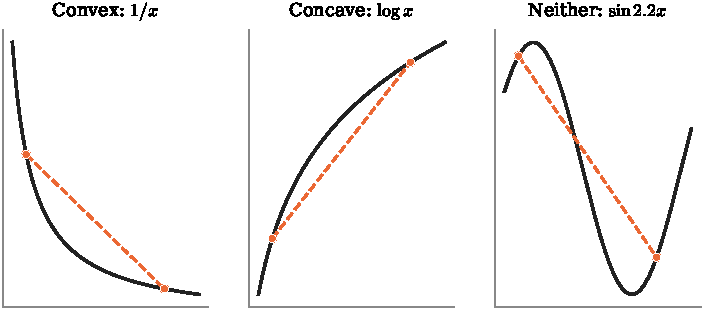
\includegraphics[width=\textwidth]{fig_tk_convex}
\caption{Convex: chords above the graph. Concave: chords below. Neither: a chord can cross the graph.}
\label{fig:tk-convex}
\end{figure}

\textbf{Where the book uses it.} Jensen's inequality (\cref{thm:jensen}) is the chord statement with the two-point average replaced by an expectation; it explains why $1/\bar{T}_n$ overestimates $\lambda$ and why $\sqrt{\cdot}$ of an unbiased estimator is biased (\cref{ch:estimators}). The quadratic in the solve interval of \cref{ch:confidence-intervals} is convex, which is why the inequality holds between its roots. Likelihoods in Part IV are maximized by finding where a concave function's slope is zero.

\section{Tangent lines, the mean value theorem and Taylor's expansion}
\label{sec:math-mvt}

The derivative $g'(\theta)$ is the slope of the tangent line to the graph of $g$ at $\theta$, and the tangent line $g(\theta) + g'(\theta)(x - \theta)$ is the best straight-line stand-in for $g$ near $\theta$.
Two facts make this precise.

\textbf{The mean value theorem.}
For a smooth $g$ and any $a < b$ there is a point $c$ between them where the tangent is parallel to the chord:
\[
g(b) - g(a) = g'(c) \, (b - a) \quad \text{for some } c \in (a, b).
\]
The change in $g$ over an interval equals the slope somewhere inside the interval times the interval's length: on the left of \cref{fig:tk-mvt}, the tangent at $c$ is parallel to the chord from $a$ to $b$.
You never learn where $c$ is, and you never need to: in the delta method it is squeezed between two points that converge to $\theta$, so $g'(c)$ converges to $g'(\theta)$.

\textbf{The first-order Taylor expansion.}
Near $\theta$,
\[
g(x) = g(\theta) + g'(\theta)(x - \theta) + \text{(an error of order } (x - \theta)^2),
\]
so on a window of width $h$ around $\theta$ the tangent line is wrong by about $h^2$, which is negligible compared with the $h$-sized changes along the line.
The right of \cref{fig:tk-mvt} draws this for $g(x) = 1/x$: the shaded error is tiny on the window $\theta \pm \sigma/\sqrt{n}$ where an estimator lives, which is why the delta method can treat $g$ as linear there.
Adding the next term, $\frac12 g''(\theta)(x - \theta)^2$, gives the second-order expansion, and it too has an exact form with an unknown in-between point, \textbf{Taylor's theorem with the Lagrange remainder}: for a twice differentiable $g$,
\[
g(b) = g(a) + g'(a)(b - a) + \tfrac12 g''(c)(b - a)^2 \quad \text{for some } c \text{ between } a \text{ and } b.
\]
At a maximum, where $g'(a) = 0$, it says that the drop from the top to $b$ is exactly half a squared distance times a curvature taken somewhere in between, which is the step behind the likelihood ratio test.
The pattern continues: for a $g$ with $k + 1$ derivatives, $g(x) = \sum_{i=0}^{k} \frac{1}{i!}g^{(i)}(\theta)(x - \theta)^i + (\text{an error of order } (x - \theta)^{k+1})$, where $g^{(i)}$ is the $i$th derivative and $g^{(0)} = g$.

\begin{figure}[htbp]
\centering
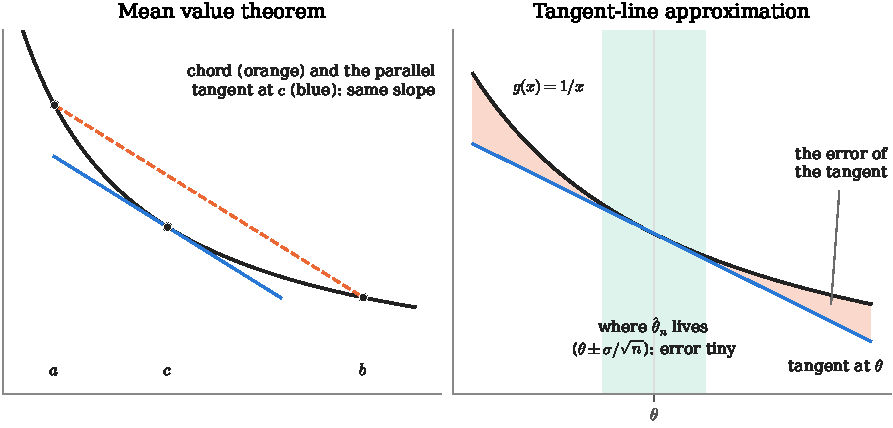
\includegraphics[width=\textwidth]{fig_tk_mvt_taylor}
\caption{Left: the mean value theorem, with the chord from $a$ to $b$ (orange) and the parallel tangent at $c$ (blue). Right: $g(x) = 1/x$ and its tangent line at $\theta$, with the error between them shaded over the window $\theta \pm \sigma/\sqrt{n}$.}
\label{fig:tk-mvt}
\end{figure}

\textbf{Where the book uses it.} The delta method (\cref{thm:delta}) is the mean value theorem followed by Slutsky's theorem; its intuition box is the tangent-line picture. The second-order expansion is behind the remark on $g'(\theta) = 0$ in \cref{sec:delta-method}, and Taylor's theorem with the Lagrange remainder proves Wilks' theorem in \cref{ch:wald-lrt}. \Cref{ex:gof-taylor} uses the terms of order three and four to compare $G^2$ with Pearson's statistic.

\section{Exponentials and logarithms}
\label{sec:math-explog}

Two facts about $e$ recur.
First, $(1 - x/n)^n \to e^{-x}$ as $n \to \infty$; the left of \cref{fig:tk-explog} shows the curves for $n = 1, 2, 5, 20$ climbing toward $e^{-x}$, each drawn up to $x = n$, where it reaches $0$. More generally $(1 + a/n)^n \to e^{a}$.
It is the step that turns the finite-$n$ formula in the maximum-of-uniforms proof (\cref{ex:max-unif}) into an exponential limit, and it reappears whenever a product of $n$ nearly-equal factors is pushed to the limit.
Second, the logarithm turns multiplication into addition, $\log(ab) = \log a + \log b$: on the right of \cref{fig:tk-explog}, equal ratios along the axis become equal steps up the curve, so a product becomes a sum.
A likelihood is a product of $n$ densities, a number so small it underflows a computer for moderate $n$; its logarithm is a sum of $n$ ordinary terms, and a sum of $n$ terms is what the Law of Large Numbers and the Central Limit Theorem know how to handle.
That is the entire reason Part IV works with log-likelihoods.
Because $\log$ is strictly increasing, maximizing the likelihood and maximizing the log-likelihood give the same answer.

\begin{figure}[htbp]
\centering
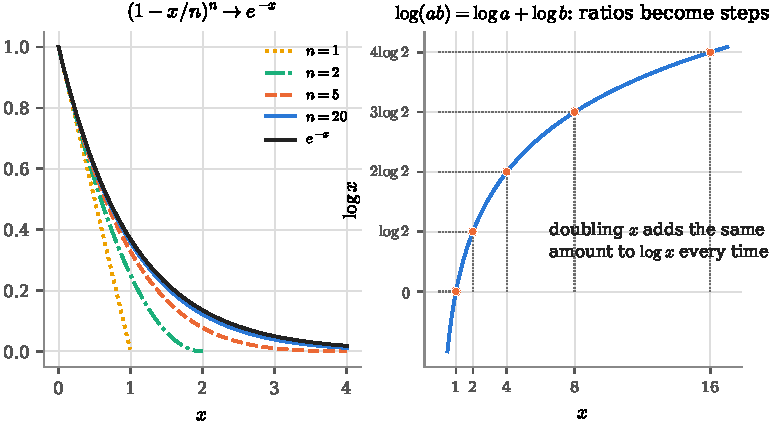
\includegraphics[width=\textwidth]{fig_tk_exp_log}
\caption{Left: $(1 - x/n)^n$ for $n = 1, 2, 5, 20$, each drawn up to $x = n$, and the limit $e^{-x}$. Right: the graph of the logarithm.}
\label{fig:tk-explog}
\end{figure}

\section{Orders of magnitude: how fast is `fast'}
\label{sec:math-rates}

The book keeps saying that an error is `of order $1/\sqrt{n}$', that a bound `goes to zero like $1/n$', or `exponentially fast'.
These are statements about how a quantity scales with $n$, ignoring constants.
\Cref{fig:tk-rates} draws the three rates that matter here on ordinary axes and on log-log axes, where a power law $n^{-c}$ is a straight line of slope $-c$ and an exponential bends away below every power law.
On ordinary axes the three look alike at first; on log-log axes $1/\sqrt{n}$ and $1/n$ are straight lines whose slopes are the exponents, and the exponential drops away below both.
Practical translation of each rate:
\begin{itemize}[nosep]
\item $1/\sqrt{n}$: four times the data halves the error; a hundred times the data buys one decimal place. This is the rate of every estimator built from an average and of every confidence interval in this book.
\item $1/n$: twice the data halves the error. Chebyshev's bound and the maximum-of-uniforms example have this rate; so does the bias of $1/\bar{T}_n$ in \cref{ch:estimators}, which is why the bias is swamped by the $1/\sqrt{n}$ standard error.
\item $e^{-cn}$: each fixed addition to $n$ multiplies the error by the same factor below $1$. Hoeffding's bound has this rate, which is why it overtakes Chebyshev's for large $n$ (\cref{fig:bounds}).
\end{itemize}

\begin{figure}[htbp]
\centering
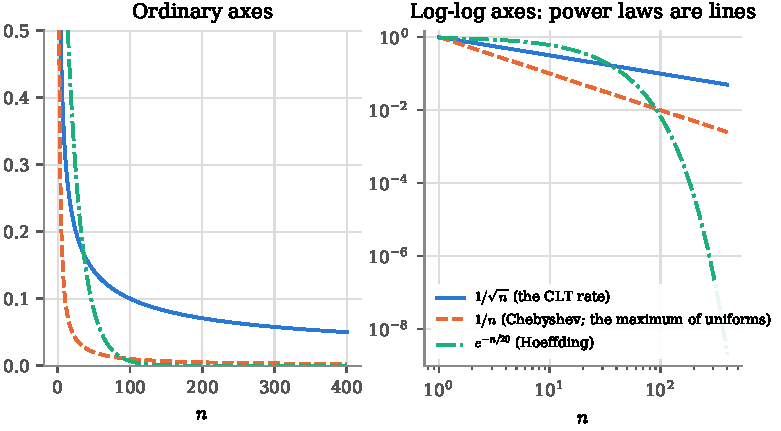
\includegraphics[width=\textwidth]{fig_tk_rates}
\caption{Three rates of decay, $1/\sqrt{n}$, $1/n$ and an exponential. Left: on ordinary axes. Right: on log-log axes.}
\label{fig:tk-rates}
\end{figure}

\section{Functions of several variables: gradient and Hessian}
\label{sec:math-multivar}

A parameter with several coordinates, like $(\mu, \sigma^2)$ for a Gaussian, turns a log-likelihood into a function of several variables, and maximizing it needs the several-variable versions of the derivative and the second derivative.

\textbf{Partial derivatives and the gradient.}
For $h(a, b)$, the partial derivative $\partial h/\partial a$ is the ordinary derivative in $a$ with $b$ held fixed: the slope of the surface walking in the $a$ direction.
The \textbf{gradient} collects them in a vector, $\nabla h = (\partial h/\partial a, \partial h/\partial b)$.
It points in the direction in which $h$ climbs fastest, it is perpendicular to the contour line through its point, and its length is the steepness of the climb.
On the left of \cref{fig:tk-gradient}, for the concave function $-(a^2 + ab + b^2)$, each arrow points uphill, perpendicular to the contour through its base, and the arrows shrink to nothing at the top, the one point where the gradient is $0$.
At the top of a hill the surface is flat in every direction, so the gradient is the zero vector: $\nabla h = 0$ is the first-order condition, one equation per coordinate.

\textbf{The Hessian and the second-derivative test.}
The \textbf{Hessian} is the matrix of second partial derivatives,
\[
\nabla^2 h = \begin{pmatrix} \partial^2 h/\partial a^2 & \partial^2 h/\partial a\,\partial b \\ \partial^2 h/\partial b\,\partial a & \partial^2 h/\partial b^2 \end{pmatrix},
\]
which is symmetric for the smooth functions of this book.
A zero gradient alone does not certify a maximum: the saddle $h(a, b) = a^2 - b^2$ has $\nabla h = 0$ at the origin, which is a minimum along $a$ and a maximum along $b$ (\cref{fig:tk-gradient}, right).
The second-derivative test settles it.
A symmetric matrix $H$ is \textbf{negative definite} if $u^\top H u < 0$ for every nonzero vector $u$: the function curves down in every direction.
If at a point where $\nabla h = 0$ the Hessian is negative definite, the point is a local maximum.
For a $2 \times 2$ Hessian, negative definite means the top-left entry is negative and the determinant is positive.
For the saddle the Hessian is $\begin{pmatrix} 2 & 0 \\ 0 & -2 \end{pmatrix}$, whose determinant is $-4$: not negative definite.
For $h(a, b) = -(a^2 + ab + b^2)$ it is $\begin{pmatrix} -2 & -1 \\ -1 & -2 \end{pmatrix}$, top-left $-2 < 0$, determinant $3 > 0$: negative definite, and the origin is the maximum.

\textbf{Concave in several variables.}
Along the line $\theta + tu$, the function $t \mapsto h(\theta + tu)$ has first derivative $\nabla h(\theta + tu)^\top u$ and second derivative $u^\top \nabla^2 h(\theta + tu)\, u$, by the chain rule.
Suppose the Hessian is negative definite at every point of a domain that contains the segment between any two of its points. Then the second derivative along every line is negative, so every slice through the function, in every direction, is strictly concave in one variable. If $\nabla h(\hat{\theta}) = 0$, the slice from $\hat{\theta}$ toward any other point $\theta$ has zero slope at $\hat{\theta}$, so by the one-variable result (\cref{prop:concave-max}) it is highest there: $h(\theta) < h(\hat{\theta})$. A point with zero gradient, if there is one, is the unique maximizer, exactly as in one variable.

\begin{figure}[htbp]
\centering
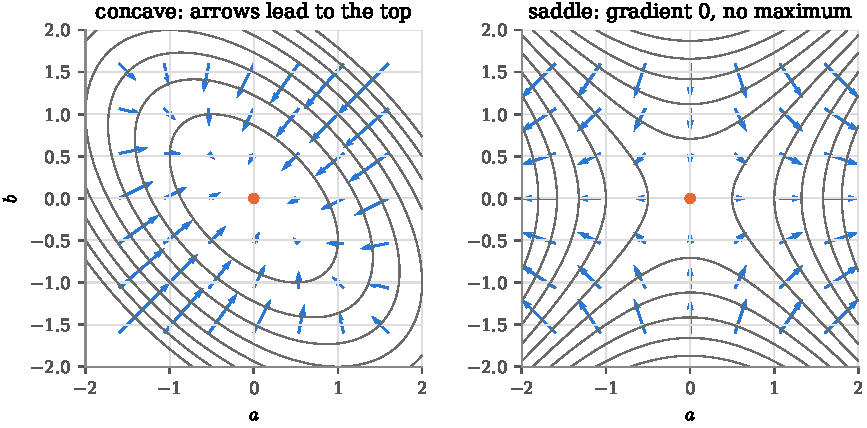
\includegraphics[width=\textwidth]{fig_tk_gradient}
\caption{Left: contours of $h(a, b) = -(a^2 + ab + b^2)$, with the gradient drawn as an arrow at a grid of points. Right: the saddle $h(a, b) = a^2 - b^2$.}
\label{fig:tk-gradient}
\end{figure}

\textbf{Where the book uses it.} The Gaussian maximum likelihood estimator (\cref{sec:lik-families}) is found by a two-step argument, and its Hessian at the maximum is negative definite; the EM algorithm (\cref{sec:lik-em}) maximizes in five coordinates; \cref{ch:mle-properties} turns the Hessian of the log-likelihood into the Fisher information matrix.

\section{Vectors of independent Gaussians and rotations}
\label{sec:math-gaussvec}

Cochran's theorem (\cref{thm:cochran}) rests on one fact: a vector of independent standard Gaussians looks the same after any rotation of the axes.
Three pieces of calculus and linear algebra make it precise.

\textbf{Joint densities.}
If $Z_1, \ldots, Z_n$ are independent continuous random variables with densities $f_1, \ldots, f_n$, the vector $Z = (Z_1, \ldots, Z_n)$ has the joint density $f(z) = f_1(z_1)\cdots f_n(z_n)$ on $\real^n$: the probability that $Z$ lands in a region is the integral of $f$ over it, and the product form is what independence means for densities.
Conversely, if a joint density factors as a product of a function of $z_1$ alone, a function of $z_2$ alone and so on, the coordinates are independent, each with the density its factor gives after normalizing.
For i.i.d.\ standard Gaussians,
\[
f(z) = \prod_{i=1}^n \frac{1}{\sqrt{2\pi}}e^{-z_i^2/2} = (2\pi)^{-n/2}\exp\Big(-\frac{\norm{z}^2}{2}\Big), \qquad \norm{z}^2 = z_1^2 + \cdots + z_n^2.
\]
The density depends on $z$ only through its length $\norm{z}$, so it is the same at every point of a sphere around the origin: the cloud of draws is round (\cref{fig:gaussrotation}).

\textbf{Orthogonal matrices.}
An $n \times n$ matrix $Q$ is \textbf{orthogonal} if $Q^\top Q = I$, which says that its columns are unit vectors perpendicular to each other: an orthonormal basis of $\real^n$ written as a matrix. Since $Q$ is square, $Q^\top Q = I$ makes $Q^\top$ the inverse of $Q$, so $QQ^\top = I$ as well: the rows are orthonormal too, and $Q^\top$ is itself orthogonal.
Multiplying by $Q$ rotates (and possibly reflects) the axes.
Two consequences: $Q$ preserves lengths, $\norm{Qz}^2 = (Qz)^\top(Qz) = z^\top Q^\top Q z = \norm{z}^2$, and $\det Q = \pm 1$, since $\det(Q^\top Q) = (\det Q)^2 = 1$.
Any unit vector $u_1$ can be made the first row of an orthogonal matrix: extend it to a basis of $\real^n$ and run the Gram--Schmidt process, which subtracts from each new vector its components along the previous ones and normalizes, producing an orthonormal basis $u_1, \ldots, u_n$ that keeps $u_1$ as it is; the same process keeps any orthonormal $u_1, \ldots, u_k$ as the first $k$ rows.
The proof of \cref{thm:cochran} uses $u_1 = (1, \ldots, 1)/\sqrt{n}$.

\textbf{Change of variables for a linear map.}
If $Z$ has density $f$ on $\real^n$ and $A$ is an invertible $n \times n$ matrix, then $Y = AZ$ has density
\[
f_Y(y) = \frac{f(A^{-1}y)}{\abs{\det A}}.
\]
This is the substitution rule of multivariable calculus: a linear map multiplies every volume by $\abs{\det A}$, so the probability $f(z)\,\mathrm{d}z$ of a small box around $z$ is spread over a box of volume $\abs{\det A}\,\mathrm{d}z$ around $y = Az$.
For $n = 1$ it is the familiar $f_Y(y) = f(y/a)/\abs{a}$ for $Y = aZ$, the affine property of \cref{ch:gaussian}.

\textbf{Rotation invariance.}
Put the three together.
Let $Z$ have i.i.d.\ $\Gauss(0,1)$ coordinates and $Q$ be orthogonal, and set $Y = QZ$.
Then $A^{-1} = Q^{-1} = Q^\top$, $\abs{\det Q} = 1$, and $\norm{Q^\top y} = \norm{y}$, so
\[
f_Y(y) = (2\pi)^{-n/2}\exp\Big(-\frac{\norm{Q^\top y}^2}{2}\Big) = (2\pi)^{-n/2}\exp\Big(-\frac{\norm{y}^2}{2}\Big) = \prod_{i=1}^n \frac{1}{\sqrt{2\pi}}e^{-y_i^2/2}.
\]
The density of $Y$ is the same product, so $Y_1, \ldots, Y_n$ are again i.i.d.\ $\Gauss(0,1)$, and $\norm{Y} = \norm{Z}$.
In words: rotate a round Gaussian cloud and you get the same round Gaussian cloud, with the new coordinates as independent as the old ones.
\Cref{ex:t-cochran-two} does the computation by hand for $n = 2$ and the $45^\circ$ rotation.

\textbf{Where the book uses it.} \Cref{thm:cochran} rotates the standardized data so that one coordinate is $\sqrt{n}\bar{Z}_n$ and the others carry the deviations; \cref{thm:pearson} rotates the standardized deviations of the counts with an orthogonal matrix whose first row is $(\sqrt{p^0_1}, \ldots, \sqrt{p^0_K})$, the direction in which those deviations cannot move; \cref{thm:reg-exact} rotates the errors of a regression with the first two axes along $(1, \ldots, 1)$ and along the centered explanatory values; \cref{ch:regression-multi} uses the same rotation with the regressors' subspace in place of the line through $(1, \ldots, 1)$.

\section{Gaussian vectors with a covariance matrix}
\label{sec:math-gaussquad}

The limits in \cref{ch:mle-properties,ch:mom-mestimation,ch:wald-lrt} are Gaussian vectors whose coordinates have different variances and are correlated.
This entry says what such a vector is, building on the round Gaussian cloud of the previous entry, and proves the facts the book uses about it.

\textbf{Covariance matrices.}
For a random vector $Z = (Z_1, \ldots, Z_d)$ with finite variances, the covariance matrix $\cov(Z)$ has entries $\cov(Z_j, Z_k)$, with the variances on the diagonal.
For a matrix $B$, $\cov(BZ) = B\,\cov(Z)\,B^\top$: each entry is the covariance of two linear combinations of the $Z_j$, expanded term by term.
A covariance matrix $\Sigma$ is symmetric, and $a^\top\Sigma a = \var(a^\top Z) \geq 0$ for every vector $a$.
It is \textbf{positive definite} when $a^\top\Sigma a > 0$ for every $a \neq 0$, that is, when no nonzero linear combination of the coordinates is constant; a positive definite matrix is invertible, since $\Sigma a = 0$ would give $a^\top\Sigma a = 0$.
Conversely, an invertible covariance matrix is positive definite.
If $a^\top\Sigma a = \var(a^\top Z) = 0$, then $a^\top Z$ is constant, so $(\Sigma a)_j = \cov(Z_j, a^\top Z) = 0$ for every $j$; that is, $\Sigma a = 0$, and invertibility forces $a = 0$.
The inverse of a positive definite matrix is positive definite too: for $a \neq 0$, $b = \Sigma^{-1}a$ is not $0$, and $a^\top\Sigma^{-1}a = b^\top\Sigma b > 0$.
The Fisher information matrix is the covariance matrix of the score (\cref{def:fisher}), so when it is invertible it is positive definite, and so is its inverse.

\textbf{Definition.}
Let $m \in \real^d$ and let $\Sigma$ be a symmetric positive definite $d \times d$ matrix.
A random vector $Z$ has the \textbf{Gaussian distribution} $\Gauss_d(m, \Sigma)$ if it has the distribution of $m + AW$, where $W$ has $d$ independent $\Gauss(0, 1)$ coordinates and $A$ is an invertible $d \times d$ matrix with $AA^\top = \Sigma$.
The definition concerns only the distribution of $Z$, which is all that a limit in distribution, such as the one in the Central Limit Theorem, delivers.
Such an $A$ exists for every positive definite $\Sigma$; one choice is the lower-triangular matrix of the Cholesky factorization, a standard result of linear algebra, and for $d = 2$ it is explicit: for $\Sigma = \begin{pmatrix} a & b \\ b & c\end{pmatrix}$, $A = \begin{pmatrix} \sqrt{a} & 0 \\ b/\sqrt{a} & \sqrt{c - b^2/a}\end{pmatrix}$.
$\cov(Z) = A\,\cov(W)A^\top = AA^\top = \Sigma$, and every nonzero linear combination $a^\top Z$ has the distribution of $a^\top m + (A^\top a)^\top W$, a sum of independent Gaussians plus a constant, so it is $\Gauss(a^\top m, a^\top\Sigma a)$ by the sum rule and the affine property of \cref{ch:gaussian}.
That is the description of $\Gauss_d$ used in the recall lines of \cref{ch:mom-mestimation}.
(Conversely, a vector all of whose linear combinations are Gaussian, with positive definite covariance matrix, has this form; the proof uses characteristic functions, which this book does not develop, and nothing in the book needs it.)

\textbf{The distribution depends on $A$ only through $\Sigma$.}
By the change of variables formula of the previous entry, with $f$ the density of $W$,
\[
f_Z(z) = \frac{f\big(A^{-1}(z - m)\big)}{\abs{\det A}} = \frac{1}{(2\pi)^{d/2}\abs{\det A}}\exp\Big(-\tfrac12\norm{A^{-1}(z - m)}^2\Big).
\]
Now $\norm{A^{-1}(z - m)}^2 = (z - m)^\top(A^{-1})^\top A^{-1}(z - m) = (z - m)^\top(AA^\top)^{-1}(z - m)$, and $\abs{\det A} = \sqrt{\det(AA^\top)}$, so
\[
f_Z(z) = \frac{1}{(2\pi)^{d/2}\sqrt{\det\Sigma}}\exp\Big(-\tfrac12(z - m)^\top\Sigma^{-1}(z - m)\Big),
\]
a formula with only $m$ and $\Sigma$ in it: two choices of $A$ with the same $AA^\top$ give the same distribution.
For $d = 1$ it is the Gaussian density of \cref{ch:gaussian}.
The contours of the density are the ellipses $(z - m)^\top\Sigma^{-1}(z - m) = \text{constant}$, drawn in \cref{fig:gaussquad}.

\textbf{Linear maps.}
If $Z \sim \Gauss_d(m, \Sigma)$ and $B$ is a $k \times d$ matrix of rank $k$ (its rows are linearly independent), then $BZ \sim \Gauss_k(Bm, B\Sigma B^\top)$.
To see it, note that $BZ$ has the distribution of $Bm + CW$ with $C = BA$, a $k \times d$ matrix of rank $k$, since $A$ is invertible.
Run the Gram--Schmidt process on the rows of $C$ to get orthonormal vectors $q_1, \ldots, q_k$ spanning the same space, and let $Q_1$ be the $k \times d$ matrix with these rows.
Each row of $C$ is a combination of $q_1, \ldots, q_k$, so $C = LQ_1$ with $L = CQ_1^\top$, a $k \times k$ matrix; it is invertible, since $k = \mathrm{rank}\,C = \mathrm{rank}(LQ_1) \leq \mathrm{rank}\,L$.
Extend $q_1, \ldots, q_k$ to a basis of $\real^d$ and continue the Gram--Schmidt process, as in the previous entry, to get an orthogonal matrix $Q$ whose first $k$ rows are $q_1, \ldots, q_k$.
By rotation invariance $QW$ has independent standard Gaussian coordinates, and $W' = Q_1W$ is its first $k$ of them.
So $BZ$ has the distribution of $Bm + LW'$, with $L$ invertible and $LL^\top = LQ_1Q_1^\top L^\top = CC^\top = B\Sigma B^\top$, which is the definition.

\textbf{The quadratic form.}
If $Z \sim \Gauss_d(m, \Sigma)$, then $(Z - m)^\top\Sigma^{-1}(Z - m)$ has the distribution of $W^\top A^\top(AA^\top)^{-1}AW = W^\top W$, which is $\chi^2_d$ (\cref{lem:gauss-quadform}): the squared distance from the center in units of the noise, which \cref{fig:gaussquad} draws.

\textbf{Where the book uses it.} The multivariate CLT and the asymptotic normality of estimators with several coordinates (\cref{ch:limit-tools,ch:mle-properties,ch:mom-mestimation}) have $\Gauss_d$ limits when their covariance matrices are positive definite. The quadratic form gives the chi-squared limits of Wald's, the likelihood ratio and the score tests (\cref{ch:wald-lrt}), and the linear-map rule gives the common limit of all three with nuisance parameters (\cref{thm:three-nuisance}). The vector of counts in \cref{ch:gof}, whose coordinates add up to $n$, has a covariance matrix that is not positive definite; that chapter rotates the standardized deviations of the counts so that the direction in which they cannot move is one coordinate and sets it aside (\cref{thm:pearson}), and for the three tests drops one category (\cref{sec:gof-score}); either way the covariance matrix that remains is positive definite.

\section{Conditional distributions and conditional expectation}
\label{sec:math-condexp}

For a pair $(X, Y)$ with a joint density $h(x, y)$, the \textbf{marginal density} of $X$ is $h(x) = \int h(x, y)\,\mathrm{d}y$, and wherever $h(x) > 0$ the \textbf{conditional density} of $Y$ given $X = x$ is
\[
h(y \mid x) = \frac{h(x, y)}{h(x)}:
\]
the slice of the joint density along the vertical line at $x$, rescaled so that it integrates to $1$.
For discrete pairs, PMFs replace densities and sums replace integrals: $\Pr(Y = y \mid X = x) = \Pr(X = x, Y = y)/\Pr(X = x)$.
The \textbf{conditional expectation} $\E[Y \mid X = x] = \int y\,h(y \mid x)\,\mathrm{d}y$ is the mean of that slice, one number for each $x$.
\Cref{fig:tk-condexp} draws the simplest case: two dice, $X$ the first and $Y$ the sum. Given $X = x$, the sum is $x + d$ with $d = 1, \ldots, 6$ equally likely, so $\E[Y \mid X = x] = x + 3.5$.

\begin{figure}[htbp]
\centering
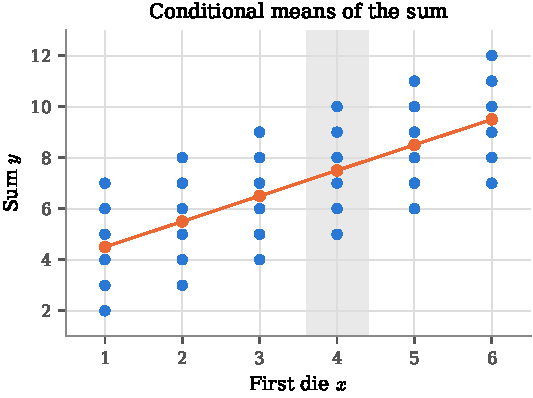
\includegraphics[width=0.6\textwidth]{fig_tk_condexp}
\caption{Two dice: the $36$ equally likely outcomes as points (first die, sum), and the conditional means of the sum given the first die (orange); the shaded column holds the six outcomes with first die $4$.}
\label{fig:tk-condexp}
\end{figure}

Writing $f(x) = \E[Y \mid X = x]$, the random variable $f(X)$, the conditional mean evaluated at the observed $X$, is written $\E[Y \mid X]$. Three facts handle it.
\begin{itemize}[nosep]
\item \textbf{The tower property}: $\E\big[\E[Y \mid X]\big] = \E[Y]$. For densities, $\E[f(X)] = \int f(x)h(x)\,\mathrm{d}x = \iint y\,h(y \mid x)h(x)\,\mathrm{d}y\,\mathrm{d}x = \iint y\,h(x, y)\,\mathrm{d}y\,\mathrm{d}x = \E[Y]$. For the dice, the average of $x + 3.5$ over $x = 1, \ldots, 6$ is $7$, the mean of the sum.
\item \textbf{Taking out what is known}: $\E[g(X)Y \mid X] = g(X)\E[Y \mid X]$ for any function $g$ with $\E\abs{g(X)Y} < \infty$: once $X = x$ is fixed, $g(x)$ is a constant and comes out of the mean of the slice. With the tower property, $\E[g(X)Y] = \E\big[g(X)\E[Y \mid X]\big]$.
\item \textbf{Conditional variance}: $\var(Y \mid X = x) = \E[Y^2 \mid X = x] - \big(\E[Y \mid X = x]\big)^2$ is the variance of the slice, so it is non-negative; hence $\E[Y \mid X]^2 \leq \E[Y^2 \mid X]$, and by the tower property $\E\big[\E[Y \mid X]^2\big] \leq \E[Y^2]$.
\end{itemize}

\textbf{Where the book uses it.} The posterior of \cref{ch:bayes-intro} is a conditional density of the parameter given the data; the regression function of \cref{ch:regression-uni} is a conditional expectation, and the proof that it is the best predictor (\cref{thm:best-predictor}) uses all three facts.

\section{Matrices, rank and projections}
\label{sec:math-matrices}

\Cref{ch:regression-multi} writes $n$ regression equations as one, $Y = X\beta + \epsilon$, and solves them by geometry.
This entry collects the linear algebra that takes.

\textbf{Vectors and matrices.}
A vector $v \in \real^n$ is a column of $n$ numbers; $v^\top$ is the same numbers as a row, so $u^\top v = \sum_i u_iv_i$ is a number, the inner product, and $\norm{v}^2 = v^\top v$ is the squared length.
Two vectors are \textbf{perpendicular} (orthogonal) when $u^\top v = 0$, and then $\norm{u + v}^2 = \norm{u}^2 + \norm{v}^2$ (Pythagoras: the cross term $2u^\top v$ vanishes).
An $n \times p$ matrix $X$ sends $\beta \in \real^p$ to $X\beta \in \real^n$, which is the combination $\beta_1x_{(1)} + \cdots + \beta_px_{(p)}$ of the columns of $X$ with the entries of $\beta$ as weights.
The transpose rule $(AB)^\top = B^\top A^\top$ and the inverse rule $(AB)^{-1} = B^{-1}A^{-1}$ hold whenever the products and inverses exist; the \textbf{trace} $\mathrm{tr}(A)$ of a square matrix is the sum of its diagonal entries, $\mathrm{tr}(AB) = \mathrm{tr}(BA)$ whenever both products are square, and $\mathrm{tr}$ is linear, so it passes through expectations.

\textbf{Column space and rank.}
The \textbf{column space} of $X$ is the set of all vectors $X\beta$, a subspace of $\real^n$ (closed under sums and multiples).
The columns are \textbf{linearly independent} when $X\beta = 0$ only for $\beta = 0$, that is, when no column is a combination of the others; then every vector in the column space is $X\beta$ for exactly one $\beta$, and the column space has dimension $p$.
The \textbf{rank} of $X$ is the dimension of its column space, so `rank $p$' with $p \leq n$ means the columns are independent.
Independent columns make $X^\top X$ invertible: $X^\top Xa = 0$ gives $a^\top X^\top Xa = \norm{Xa}^2 = 0$, so $Xa = 0$ and $a = 0$.

\textbf{Orthogonal projection.}
Let $S$ be a subspace of $\real^n$ of dimension $d$. The Gram--Schmidt process of \cref{sec:math-gaussvec}, fed a basis of $S$ and then vectors completing it to a basis of $\real^n$, gives an orthonormal basis $u_1, \ldots, u_n$ of $\real^n$ whose first $d$ vectors span $S$; fed a basis of a smaller subspace $S_0 \subset S$ first, it gives one adapted to the chain $S_0 \subset S \subset \real^n$.
Every $y$ then splits as $y = s + r$ with $s = \sum_{k \leq d}(u_k^\top y)u_k \in S$ and $r = \sum_{k > d}(u_k^\top y)u_k$ perpendicular to every vector of $S$, and uniquely, since two such splits would differ by a vector of $S$ perpendicular to $S$, which is $0$; $s$ is the \textbf{orthogonal projection} of $y$ onto $S$, and it is the point of $S$ closest to $y$, since for any $s' \in S$, $\norm{y - s'}^2 = \norm{r}^2 + \norm{s - s'}^2 \geq \norm{r}^2$ by Pythagoras.
\Cref{fig:tk-projection} draws the case of a line.
The map $y \mapsto s$ is linear, so it is a matrix $P$, with $P^2 = P$ (projecting twice changes nothing) and $P^\top = P$; for $S$ the column space of a rank-$p$ matrix $X$, the condition that $y - Py$ be perpendicular to every column reads $X^\top(y - Xb) = 0$, whose solution $b = (X^\top X)^{-1}X^\top y$ gives
\[
P = X(X^\top X)^{-1}X^\top, \qquad \mathrm{tr}(P) = \mathrm{tr}\big((X^\top X)^{-1}X^\top X\big) = p.
\]
$I - P$ is the projection onto the \textbf{orthogonal complement} of $S$, the vectors perpendicular to $S$, a subspace of dimension $n - p$.
In the adapted basis, $P = \sum_{k \leq d}u_ku_k^\top$, so if $S_0 \subset S$ are nested subspaces of dimensions $d_0 \leq d$ with projections $P_0 = \sum_{k \leq d_0}u_ku_k^\top$ and $P$, then $PP_0 = P_0$, and $P - P_0 = \sum_{d_0 < k \leq d}u_ku_k^\top$ is the projection onto the span of $u_{d_0+1}, \ldots, u_d$, the part of $S$ perpendicular to $S_0$, of dimension $d - d_0$.

\begin{figure}[htbp]
\centering
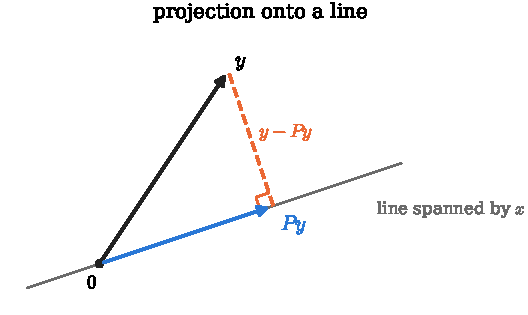
\includegraphics[width=0.5\textwidth]{fig_tk_projection}
\caption{Orthogonal projection onto a line: the vector $y$ (black), the line spanned by $x$ (gray), the projection $Py$ (blue) and the residual $y - Py$ (orange, dashed), perpendicular to the line.}
\label{fig:tk-projection}
\end{figure}

\textbf{Where the book uses it.} Least squares is the projection of the response onto the column space of the design matrix (\cref{thm:mreg-lse}); the residual sum of squares has $n - p$ degrees of freedom because $I - P$ projects onto an $(n - p)$-dimensional space (\cref{thm:mreg-exact}); the $F$-test splits the column space into nested pieces (\cref{thm:mreg-ftest}); and full rank is the identifiability of the regression model (\cref{ch:models}).

\section{To be added with later chapters}
\label{sec:math-later}

Eigenvalues and eigenvectors (for \cref{ch:pca}).

\chapter{The Modes of Convergence in Full}
\label{app:modes}

\Cref{ch:lln,ch:clt} used two modes of convergence, in probability and in distribution: the Law of Large Numbers lives in the first and the Central Limit Theorem in the second.
There is a third, almost sure convergence, and a fourth, convergence in mean; all four can be ranked by strength.
Nothing later in the book is proved with the two extra modes, which is why they're here rather than in the main sequence; where a later chapter mentions almost sure convergence, as \cref{ch:limit-tools,ch:estimators} do, the in-probability version is the one in use.
This appendix is for orientation, and for the reader who wants to know what the Strong Law of Large Numbers actually says.

\section{Intuition for the three main modes}
\label{sec:conv-intuition}

\begin{enumerate}
\item \textbf{Convergence in probability:}
Imagine you have a sequence of r.v.s (like a sequence of coin flips or dice rolls).
If this sequence converges in probability to a specific value, it means that as you progress through the sequence, the probability of the r.v.s being `close' to that specific value tends to 1.
In other words, with enough trials you can make it as likely as you please that the result is close to the value the sequence is converging to.

\item \textbf{Almost sure convergence (convergence almost surely):}
Almost sure convergence is a stronger notion than convergence in probability.
If a sequence of r.v.s converges almost surely to a value, it means that the probability of the sequence eventually staying close to that value is 1.
More concretely, if you were to run the experiment and watch the whole infinite sequence unfold, the sequence you see converges, in the plain calculus sense, with probability 1.
Almost sure convergence implies convergence in probability, but not conversely.
Given that a sequence of r.v.s converging almost surely means that it converges to the value with probability 1, this mode of convergence is the closest analog to convergence of sequences of numbers as studied in calculus; it's a deterministic understanding of convergence applied one outcome at a time.

\item \textbf{Convergence in distribution:}
Convergence in distribution is a weaker notion compared to the previous two.
It doesn't focus on the actual values of the random variables but rather on their distribution.
If a sequence of r.v.s converges in distribution to an r.v., it means that the shape of the distribution of the sequence becomes increasingly similar to the distribution of the limiting r.v.
In simpler terms, the probabilities of the sequence falling within certain ranges will approximate the probabilities of the limiting variable falling within the same ranges.
\end{enumerate}

The modes come in the order the book uses them. Convergence in probability first since the Law of Large Numbers lives there and it's where estimators are shown to work; convergence in distribution second since the Central Limit Theorem lives there and it's where confidence intervals and tests come from; and almost sure convergence last since the Strong Law is worth stating on its own account and is never needed again.

\section{Convergence almost surely}
\label{sec:conv-as}

Like convergence in probability, convergence almost surely involves a limiting process between random variables, say $X_n$ and $X$, that live on the same sample space.
Unlike convergence in probability, though, the limiting process for almost sure convergence is located \textit{within} the probability measure.
Compare the two definitions side by side:
\begin{align*}
\text{in probability:} \qquad & \lim_{n \to \infty} \Pr \left( \abs{X_n - X} \geq \epsilon \right) = 0 \quad \text{for every } \epsilon > 0, \\
\text{almost surely:} \qquad & \Pr \left( \lim_{n \to \infty} X_n = X \right) = 1.
\end{align*}

In the first, you compute a probability for each $n$ and then take a limit of numbers.
In the second, you fix an outcome $s$ of the experiment, which fixes the entire sequence of numbers $X_1(s), X_2(s), \ldots$, ask whether that sequence of numbers converges to the number $X(s)$ in the calculus sense, and then ask for the probability of the set of outcomes for which the answer is yes.

\begin{definition}[Convergence almost surely]
\label{def:convas}
Let $(X_n)_{n \geq 1}$ be a sequence of r.v.s defined on a sample space $S$.
The sequence \textbf{converges almost surely} to an r.v.\ $X$ if:
\[
\Pr \left( \left\{ s \in S : \lim_{n \to \infty} X_n(s) = X(s) \right\} \right) = 1.
\]
If $(X_n)_{n \geq 1}$ converges almost surely to the r.v.\ $X$, this is denoted by $X_n \convas X$.
\end{definition}

\begin{inwords}
\textbf{In words.} Run the experiment once and watch the whole infinite sequence of numbers it produces; with probability one, that sequence converges in the plain calculus sense \toolkit{sec:math-limits}. The set of runs where it fails is allowed to be nonempty, as long as it has probability zero \toolkit{sec:math-rv}.
\par\smallskip
\textbf{For the kiss data.} Keep observing couples forever and keep updating the running proportion; the Strong Law says the running proportion settles on $p$ and stays there, for all but a probability-zero set of infinite runs.
\end{inwords}

`Almost surely' is probability's phrase for `with probability 1'.
The set of outcomes on which the sequence fails to converge is allowed to be nonempty, as long as it has probability $0$.

\begin{example}
\label{ex:as-uniform-power}
Let $U \sim \text{Unif}([0, 1])$ and define $X_n = U + U^n$.
For every outcome with $U \in [0, 1)$, $U^n \to 0$ as $n \to \infty$, so $X_n \to U$.
For the outcome $U = 1$ the sequence is constant at $2$ and does not converge to $U = 1$.
But $\Pr(U = 1) = 0$, so $\Pr(X_n \to U) = \Pr(U \in [0,1)) = 1$ and $X_n \convas U$.
This is the sense in which `almost' is used: convergence can fail on a set of outcomes, provided that set has probability zero.
\end{example}

\subsection{The Strong Law of Large Numbers (SLLN)}

\begin{theorem}[Strong Law of Large Numbers]
\label{thm:slln}
Let $X_1, X_2, \ldots$ be i.i.d.\ r.v.s with $\E\abs{X_i} < \infty$ and $\E[X_i] = \mu$.
Then:
\[
\bar{X}_n \convas \mu.
\]
\end{theorem}

Two things are notable about the statement.
First, it requires only a finite mean, not a finite variance; the Weak Law was proved in \cref{ch:lln} using Chebyshev's inequality, which needs the variance, but the conclusion of both laws holds under the weaker assumption.
Second, the conclusion is about sample paths: run the experiment once, forever, and the sequence of running averages you record converges to $\mu$, with probability one.
\Cref{fig:sllnpaths} shows six such paths for a fair coin.
The two laws are often written together as
\[
\bar{X}_n \convasp \mu,
\]
allowing whichever one is convenient to be used; for everything in this book the Weak Law of \cref{ch:lln} is enough.

\begin{figure}[htbp]
\centering
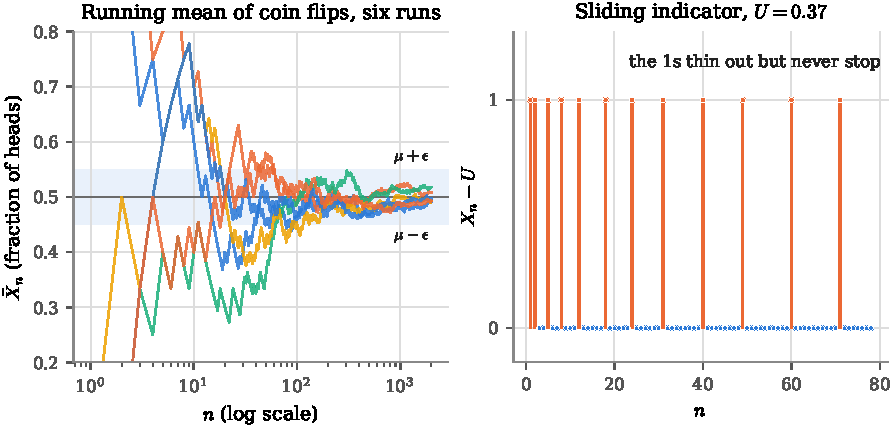
\includegraphics[width=\textwidth]{fig_slln_paths}
\caption{Left: six realizations of the running proportion of heads in a fair coin, on a logarithmic $n$ axis. Each path wanders early, enters the band $\mu \pm 0.05$ and, as the Strong Law says, stays there; with probability one every path eventually does this. Right: one outcome of the sliding-indicator sequence of \cref{ex:sliding}, which converges in probability but not almost surely. For this outcome ($U = 0.37$) the value $1$ keeps recurring, at ever longer intervals, forever.}
\label{fig:sllnpaths}
\end{figure}

\subsection{Convergence almost surely versus convergence in probability}

While the Weak Law of Large Numbers illustrates convergence in probability and the Strong Law of Large Numbers shows convergence almost surely, what's the difference between the two?
The following provides some intuition on the distinction between these two modes of convergence.

Suppose you have some device that improves over time.
So every time you use the device the probability of it failing is less than before.

Convergence in probability says that the chance of failure goes to zero as the number of usages goes to infinity.
So after using the device a large number of times, you can be very confident of it working correctly; it still might fail, but that's very unlikely.

On the other hand, convergence almost surely is a bit stronger.
It says that the total number of failures is \textit{finite}.
That is, if you count the number of failures as the number of usages goes to infinity, you will get a finite number.
The impact of this is as follows: As you use the device more and more, you will, after some finite number of usages, exhaust all failures.
From then on the device will work perfectly.
You don't actually know when you have exhausted all failures, so from a purely practical point of view, there isn't much difference between the two modes of convergence.

It's a good thing that the Strong Law of Large Numbers exists, as opposed to just the Weak Law.
For example, a scientific experiment is justified in taking averages: after obtaining enough data, you can get arbitrarily close to the true average, and there will be only finitely many failures (however improbable) in the averaging process, after which the average stays close.

Here is what `failures (however improbable) in the averaging process' means.
Choose some $\delta > 0$ arbitrarily small.
You obtain $n$ estimates $\Xton$ of some other quantity that has some `true' value, say $\mu$.
You compute the average:
\[
S_n = \frac{1}{n} \sum_{i = 1}^n X_i.
\]

As you obtain more data ($n$ increases) you can compute $S_n$ for $n=1,2,\ldots$.
The Weak Law says (under some assumptions about the $X_n$) that the probability $\Pr( \abs{S_n - \mu } > \delta ) \to 0$, as $n$ goes to $\infty$.
The Strong Law says that the number of times that $\abs{S_n - \mu }$ is larger than $\delta$ is finite (with probability 1).
That is, if we define the indicator function $\ind(\abs{S_n - \mu } > \delta )$ that returns one when $\abs{S_n - \mu } > \delta$ and zero otherwise, then
$\ds \sum_{n=1}^{\infty} \ind(\abs{S_n - \mu } > \delta )$ is finite.
This gives you considerable confidence in the value of $S_n$ because it guarantees, with probability 1, the existence of some finite $n_0$ such that $\abs{S_n - \mu } \leq \delta$ for all $n > n_0$.
That is, the average never fails for $n > n_0$.
Note that the Weak Law gives no such guarantee: it says failures become rare, not that they stop.

The following example, from Casella and Berger, is the standard illustration of a sequence for which failures become rare but never stop.

\begin{example}[The sliding indicator]
\label{ex:sliding}
Let $U \sim \text{Unif}([0,1])$ and define
\begin{align*}
X_1 &= U + \ind(U \in [0, 1]), \\
X_2 &= U + \ind(U \in [0, \tfrac12]), \qquad X_3 = U + \ind(U \in [\tfrac12, 1]), \\
X_4 &= U + \ind(U \in [0, \tfrac13]), \qquad X_5 = U + \ind(U \in [\tfrac13, \tfrac23]), \qquad X_6 = U + \ind(U \in [\tfrac23, 1]), \\
&\ \ \vdots
\end{align*}
so the indicator's interval slides across $[0,1]$ in blocks, and the intervals in the $m$-th block have length $1/m$.
Each $X_n$ equals either $U$ or $U + 1$.
\textit{Convergence in probability holds:} for any $0 < \epsilon < 1$, $\Pr(\abs{X_n - U} \geq \epsilon) = \Pr(U \in [a_n, b_n]) = b_n - a_n$, the length of the $n$-th interval, which goes to zero.
So $X_n \convp U$.
\textit{Almost sure convergence fails:} fix any outcome $U = u$.
In every block, exactly one interval (or two, at a shared endpoint) contains $u$, so $X_n(u) - u$ equals $1$ at least once in every block, forever.
The sequence of numbers $X_n(u)$ therefore takes the value $u + 1$ infinitely often and cannot converge to $u$.
This happens for every outcome, so $\Pr(X_n \to U) = 0$, the opposite of what almost sure convergence requires.
The right panel of \cref{fig:sllnpaths} shows one outcome.
\end{example}

In the device analogy, the sliding indicator is a device whose failures get rarer and rarer but never run out.

\section{Convergence in mean}
\label{sec:conv-mean}

There's a fourth mode, which this book needs only in passing but which you've already used: the shrinking-variance criterion of \cref{prop:shrinking-variance} is a statement about it.

\begin{definition}[Convergence in $r$-th mean]
\label{def:convr}
For $r \geq 1$, a sequence $(X_n)_{n \geq 1}$ \textbf{converges in $r$-th mean} (or in $L^r$) to $X$, written $X_n \convr{r} X$, if
\[
\lim_{n \to \infty} \E \left[ \abs{X_n - X}^r \right] = 0.
\]
The case $r = 2$ is called convergence in mean square (or quadratic mean).
\end{definition}

\begin{inwords}
\textbf{In words.} The average size of the error, measured by its $r$-th power, goes to zero. For $r = 2$ this is `the quadratic risk goes to zero'.
\par\smallskip
\textbf{For the kiss data.} $\E[(\bar{R}_n - p)^2] = p(1-p)/n \to 0$, so $\bar{R}_n \to p$ in mean square; by Markov's inequality \toolkit{sec:math-inequalities} that implies convergence in probability, which is the shrinking-variance criterion of \cref{ch:lln} again.
\end{inwords}

Convergence in mean square to a constant $\mu$ is exactly the condition $\E[(X_n - \mu)^2] \to 0$, and since $\E[(X_n - \mu)^2] = \var(X_n) + (\E[X_n] - \mu)^2$ (variance plus squared bias, the identity behind the quadratic risk of \cref{ch:estimators}), it holds if and only if $\E[X_n] \to \mu$ and $\var(X_n) \to 0$.
Convergence in $r$-th mean implies convergence in probability, by Markov's inequality applied to $\abs{X_n - X}^r$:
\[
\Pr(\abs{X_n - X} \geq \epsilon) = \Pr(\abs{X_n - X}^r \geq \epsilon^r) \leq \frac{\E \abs{X_n - X}^r}{\epsilon^r} \to 0.
\]
Neither convergence in mean nor almost sure convergence implies the other.

\section{The hierarchy of convergence types}
\label{sec:conv-hierarchy}

A sequence of r.v.s might converge for one type of convergence, but not for another.
Some convergence types are `stronger' than others by which it's meant that if Type A convergence is stronger than Type B convergence, then Type A convergence implies Type B convergence.
In \cref{fig:hierarchy}, the stronger types of convergence are given at the top and as you move to the bottom the type of convergence becomes weaker.
By way of example, if a sequence of r.v.s converges in probability, then it converges in distribution as well.

\begin{figure}[htbp]
\centering
\begin{tikzpicture}[
  node distance=1.0cm and 1.6cm,
  mode/.style={draw, rounded corners=2pt, minimum width=3.6cm, minimum height=0.9cm, align=center, font=\small, fill=gray!5},
  imp/.style={-{Latex[length=2.5mm]}, thick},
  lbl/.style={font=\scriptsize, fill=white, inner sep=1pt}
]
  \node[mode] (as) {almost surely\\ $X_n \convas X$};
  \node[mode, right=of as] (lr) {in $r$-th mean\\ $X_n \convr{r} X$};
  \node[mode, below=of $(as)!0.5!(lr)$] (p) {in probability\\ $X_n \convp X$};
  \node[mode, below=of p] (d) {in distribution\\ $X_n \convd X$};
  \draw[imp] (as) -- (p);
  \draw[imp] (lr) -- (p);
  \draw[imp] (p) -- (d);
  \draw[imp, dashed, boxorange!80!black] (d.east) to[bend right=50] node[lbl, right] {only if $X$ is a constant} (p.east);
  \node[font=\scriptsize, left=0.2cm of p, align=right, text=gray] {strong};
  \node[font=\scriptsize, left=0.2cm of d, align=right, text=gray] {weak};
\end{tikzpicture}
\caption{The hierarchy. Solid arrows are implications that always hold; no solid arrow reverses. The dashed arrow is the one partial converse that matters: convergence in distribution to a \textit{constant} is the same as convergence in probability to it. Almost sure convergence and convergence in mean don't imply each other.}
\label{fig:hierarchy}
\end{figure}

Why does this hierarchy exist? Let's focus on the 3 main modes of convergence.
Consider the following points:
\begin{itemize}
\item \textbf{Almost sure convergence:} If a sequence of r.v.s converges almost surely to an r.v., it means that the probability of the sequence eventually staying close to the limiting r.v.\ is 1.
This is the strongest form of convergence because it tells us that the individual values of the r.v.s in the sequence will eventually be close to the limiting r.v.\ with probability 1.
Since the sequence eventually stays within $\epsilon$ of the limit, the probability of being more than $\epsilon$ away at time $n$ must go to zero, which is convergence in probability.

\item \textbf{Convergence in probability:} If a sequence of r.v.s converges in probability to an r.v., it means that for any given $\epsilon > 0$, the probability of the difference between the random variables in the sequence and the limiting r.v.\ being greater than $\epsilon$ goes to 0 as the sequence progresses.
This is weaker than almost sure convergence because it only tells us about the probability of the r.v.s being close to the limiting r.v.\ at each $n$ separately, not that they will eventually be close with probability 1.
The sliding indicator of \cref{ex:sliding} is the example of the gap.

\item \textbf{Convergence in distribution:} If a sequence of r.v.s converges in distribution to an r.v., it means that the cumulative distribution functions (CDFs) of the r.v.s in the sequence converge pointwise to the CDF of the limiting r.v.
This is the weakest form of convergence because it only tells us about the behavior of the distribution of the r.v.s, not about the individual values or their probabilities of being close to the limiting r.v.
If $X_n$ is close to $X$ with high probability then their CDFs must be close, which is why convergence in probability implies convergence in distribution; the $X_n = -Z$ example in the pitfall box of \cref{sec:conv-dist} shows the converse fails.
\end{itemize}


The dashed arrow in \cref{fig:hierarchy} is \cref{prop:convd-constant}: convergence in distribution to a constant is convergence in probability to it.


\section{Summary}
\label{sec:modes-summary}

\begin{center}
\small
\begin{tabular}{@{}>{\raggedright\arraybackslash}p{1.45in}>{\raggedright\arraybackslash}p{2.2in}>{\raggedright\arraybackslash}p{2.3in}@{}}
\toprule
Mode & Definition & Where it's used in this book \\
\midrule
almost surely, $X_n \convas X$ & $\Pr(X_n \to X) = 1$ & Strong Law of Large Numbers \\[4pt]
in probability, $X_n \convp X$ & $\Pr(\abs{X_n - X} \geq \epsilon) \to 0$ for every $\epsilon > 0$ & Weak LLN; consistency of estimators; the constant in Slutsky's theorem \\[4pt]
in distribution, $X_n \convd X$ & $F_{X_n}(x) \to F_X(x)$ at every continuity point of $F_X$ & CLT; confidence intervals; test statistics \\[4pt]
in $r$-th mean, $X_n \convr{r} X$ & $\E\abs{X_n - X}^r \to 0$ & shrinking-variance criterion ($r = 2$); quadratic risk \\
\bottomrule
\end{tabular}
\end{center}

\section{Exercise}

\begin{exercise}
Is the following statement correct? `If $(T_n)_{n \geq 1}$ converges in probability, then it also converges almost surely.'
\end{exercise}
\begin{solution}
No. The sliding indicator of \cref{ex:sliding} converges in probability to $U$ and almost surely to nothing.
\end{solution}

\chapter{Supplementary Proofs}
\label{app:proofs}

Some results are stated in a chapter because they explain something there, but nothing later in the book depends on them.
Their proofs are collected here so the chapters can keep moving.
Each section says where the result is stated and confirms that no later argument uses it.

\section{Pinsker's inequality}
\label{sec:proof-pinsker}

\Cref{thm:pinsker} in \cref{ch:distances} states that for any distributions $\Pr$ and $\Qr$ on the same sample space,
\[
\TV(\Pr, \Qr) \leq \sqrt{\tfrac12 \KL(\Pr, \Qr)}.
\]
It is there to say that a fit that is good in KL is good for every probability computed from it.
\textbf{Nothing later in the book depends on it}: no theorem, proof or exercise after \cref{ch:distances} uses Pinsker's inequality, and you can skip this section without losing anything.

\optionalproof{Two steps. First prove the inequality for two Bernoulli distributions, by calculus in one variable. Then show that collapsing $\Pr$ and $\Qr$ to `in the event $A^\star$ or not' turns them into two Bernoullis with the same total variation and no larger KL divergence. The second step uses the same tangent-line bound $-\log y \geq 1 - y$ as the proof that KL is nonnegative (\cref{prop:kl-properties}).}

\subsection*{Step 1: two Bernoulli distributions}

\begin{lemma}
\label{lem:pinsker-bern}
For $p, q \in (0, 1)$,
\[
\KL(\Bern(p), \Bern(q)) = p \log\frac{p}{q} + (1 - p)\log\frac{1 - p}{1 - q} \geq 2(p - q)^2.
\]
The inequality also holds for $p \in [0, 1]$ and $q \in (0, 1)$, with the convention $0 \log 0 = 0$.
\end{lemma}

\optionalproof{Fix $p$, treat the gap between the two sides as a function of $q$, and show by its derivative that it is smallest, and equal to $0$, at $q = p$.}
\begin{proof}
Fix $p$ and look at the gap as a function of $q$:
\[
g(q) = p \log\frac{p}{q} + (1 - p)\log\frac{1 - p}{1 - q} - 2(p - q)^2.
\]
At $q = p$ both terms are $0$, so $g(p) = 0$.
Differentiate in $q$:
\[
g'(q) = -\frac{p}{q} + \frac{1 - p}{1 - q} + 4(p - q).
\]
The first two terms combine over the common denominator $q(1 - q)$: $-p(1 - q) + (1 - p)q = q - p$. So
\[
g'(q) = \frac{q - p}{q(1 - q)} - 4(q - p) = (q - p)\left( \frac{1}{q(1 - q)} - 4 \right).
\]
The product $q(1 - q)$ is at most $\frac14$, since $\frac14 - q(1 - q) = (q - \frac12)^2 \geq 0$ (it is the variance of one Bernoulli observation, largest for a fair coin).
So $1/(q(1 - q)) \geq 4$ and the bracket is never negative.
The sign of $g'(q)$ is therefore the sign of $q - p$: $g$ decreases until $q = p$ and increases after.
Its smallest value is $g(p) = 0$, so $g(q) \geq 0$ for every $q$.
\end{proof}

\Cref{fig:pinsker} draws the lemma.
The divergence curve sits above the parabola $2(p - q)^2$ and touches it only at $q = p$.
Near $q = p$ the two are close: the divergence is approximately $(p - q)^2/(2p(1 - p))$ (\cref{sec:dist-kl}), and $1/(2p(1-p)) \geq 2$, with equality only for $p = \frac12$.
The parabola $2(p-q)^2$ is the divergence's own parabola for the hardest case, the fair coin, and every other Bernoulli curves up faster.

\begin{figure}[htbp]
\centering
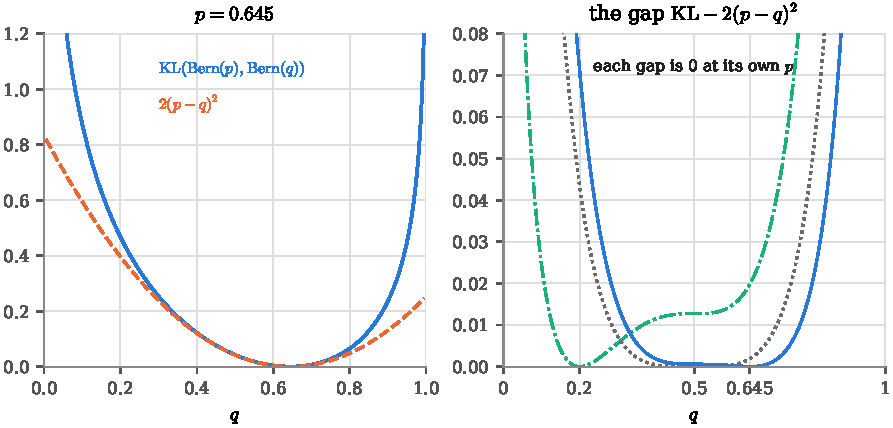
\includegraphics[width=\textwidth]{fig_pinsker}
\caption{The Bernoulli case of Pinsker's inequality. Left: with $p = 0.645$, $\KL(\Bern(p), \Bern(q))$ (blue) lies above $2(p - q)^2$ (orange, dashed) and touches it only at $q = p$. Right: the gap between the two for $p = 0.2$ (aqua, dash-dot), $0.5$ (gray, dotted) and $0.645$ (blue, solid); each gap is $0$ at $q = p$ and positive elsewhere.}
\label{fig:pinsker}
\end{figure}

For the kiss data, $p = 80/124$ and $q = \frac12$: $\KL = 0.0428$ and $2(p - q)^2 = 2 \times 0.1452^2 = 0.0422$.
Taking square roots, $\abs{p - q} = 0.1452 \leq \sqrt{0.0428/2} = 0.1462$.
Since $\TV(\Bern(p), \Bern(q)) = \abs{p - q}$, the lemma is Pinsker's inequality for Bernoulli distributions.

\subsection*{Step 2: reducing any pair of distributions to two Bernoullis}

\begin{lemma}[The log-sum inequality]
\label{lem:log-sum}
For nonnegative numbers $a_1, \ldots, a_k$ and nonnegative numbers $b_1, \ldots, b_k$ with $b_i > 0$ whenever $a_i > 0$, and with $a = \sum_i a_i > 0$ and $b = \sum_i b_i$,
\[
\sum_{i=1}^k a_i \log\frac{a_i}{b_i} \geq a \log\frac{a}{b},
\]
with the convention $0 \log 0 = 0$.
The same holds with the sums replaced by integrals over a region.
\end{lemma}

\optionalproof{Rewrite the difference of the two sides as a weighted average of $-\log$ of ratios and apply the tangent-line bound $-\log y \geq 1 - y$ to each.}
\begin{proof}
Only the terms with $a_i > 0$ contribute on the left. For those, write
\[
\sum_{i: a_i > 0} a_i \log\frac{a_i}{b_i} - a\log\frac{a}{b} = \sum_{i: a_i > 0} a_i \log\left( \frac{a_i}{b_i} \cdot \frac{b}{a} \right) = \sum_{i: a_i > 0} a_i \left[ -\log\left( \frac{b_i}{a_i} \cdot \frac{a}{b} \right) \right],
\]
using $\sum_{i: a_i > 0} a_i = a$ to bring $a\log(a/b)$ inside the sum.
Apply $-\log y \geq 1 - y$ to each bracket:
\[
\geq \sum_{i: a_i > 0} a_i \left( 1 - \frac{b_i}{a_i}\cdot\frac{a}{b} \right) = a - \frac{a}{b}\sum_{i: a_i > 0} b_i \geq a - \frac{a}{b} \cdot b = 0.
\]
The last step uses that the $b_i$ with $a_i > 0$ add up to at most $b$.
For integrals the same lines go through with $\int$ in place of $\sum$.
\end{proof}

In words: lumping several outcomes into one can only lower the divergence.
If you record only whether an outcome fell in a set, and not which outcome it was, the evidence it carries cannot go up.

\optionalproof{Collapse both distributions to the indicator of $A^\star$: total variation is unchanged, KL can only fall (\cref{lem:log-sum}), and for the two resulting Bernoullis \cref{lem:pinsker-bern} applies.}
\begin{proof}[Proof of \cref{thm:pinsker}]
If $\KL(\Pr, \Qr) = +\infty$ there is nothing to prove, so assume it is finite; then $q(x) > 0$ wherever $p(x) > 0$.
Let $A^\star = \{x : p(x) > q(x)\}$, and write $a = \Pr(A^\star)$, $b = \Qr(A^\star)$.
By \cref{prop:tv-area}, $\TV(\Pr, \Qr) = a - b$. If $a = b$, $\TV = 0$ and there is nothing to prove, so assume $a > b$; then $0 < a$ and $b < 1$.

Split the sum (or integral) defining $\KL(\Pr, \Qr)$ into the part over $A^\star$ and the part over its complement, and apply \cref{lem:log-sum} to each part, with $a_i = p(x)$ and $b_i = q(x)$:
\[
\KL(\Pr, \Qr) = \sum_{x \in A^\star} p(x)\log\frac{p(x)}{q(x)} + \sum_{x \notin A^\star} p(x)\log\frac{p(x)}{q(x)} \geq a\log\frac{a}{b} + (1 - a)\log\frac{1 - a}{1 - b}.
\]
(If a part has total $\Pr$-probability $0$, it contributes $0$ on both sides.)
The right-hand side is $\KL(\Bern(a), \Bern(b))$, the divergence between the two distributions of the indicator $\ind\{X \in A^\star\}$.
By \cref{lem:pinsker-bern} (in the extended form for $a \in [0, 1]$; if $b = 0$ the divergence on the right is $+\infty$, which contradicts the finite left side, so $b \in (0, 1)$),
\[
\KL(\Pr, \Qr) \geq \KL(\Bern(a), \Bern(b)) \geq 2(a - b)^2 = 2\,\TV(\Pr, \Qr)^2.
\]
Divide by $2$ and take square roots.
\end{proof}

\begin{intuition}[why the proof works]
Total variation is decided by one event, $A^\star$, where $\Pr$ beats $\Qr$.
Throw away everything about an outcome except whether it fell in $A^\star$.
That leaves a coin, with probability $a$ under $\Pr$ and $b$ under $\Qr$, and the same total variation $a - b$.
Lumping can only lower KL, so the coin's KL is at most the original one.
And for coins, the lemma says KL is at least twice the squared total variation.
\end{intuition}

\section{Each step of the EM algorithm raises the likelihood}
\label{sec:proof-em}

\Cref{sec:lik-em} in \cref{ch:likelihood} states that one E step followed by one M step never lowers the log-likelihood of a mixture.
It explains the climbing curves of \cref{fig:emfaithful}.
\textbf{Nothing later in the book depends on it.}

\optionalproof{Split the log-likelihood of the observed data into two pieces: the quantity the M step maximizes, minus a term that measures how well the parameter predicts the hidden labels. The M step raises the first piece. The second piece can only fall away from its value at the current parameter, by an amount that is a KL divergence and so is never negative.}

\begin{proof}
Write $\theta$ for all five parameters, $\theta_t$ for the current values and $\theta_{t+1}$ for the values after one E step and one M step.
For observation $i$, with hidden label $z \in \{0, 1\}$, let $p_\theta(x_i, z)$ be the joint probability (density in $x_i$) of the observation and the label, $p_\theta(x_i) = \sum_z p_\theta(x_i, z)$ the mixture density, and $p_\theta(z \mid x_i) = p_\theta(x_i, z)/p_\theta(x_i)$ the conditional probability of the label.
Write $q_i(z) = p_{\theta_t}(z \mid x_i)$ for the current weights: $q_i(1) = w_i$ and $q_i(0) = 1 - w_i$.

For any $\theta$ and each $z$, $\log p_\theta(x_i) = \log p_\theta(x_i, z) - \log p_\theta(z \mid x_i)$. Average this over $z$ with the weights $q_i(z)$, which add up to $1$, and add over $i$:
\[
\ell_n(\theta) = \underbrace{\sum_{i=1}^n\sum_z q_i(z)\log p_\theta(x_i, z)}_{Q(\theta)} \; - \; \underbrace{\sum_{i=1}^n\sum_z q_i(z)\log p_\theta(z \mid x_i)}_{H(\theta)}.
\]
$Q(\theta)$ is the complete-data log-likelihood with each label replaced by its weight, which is exactly what the M step maximizes over all five parameters (\cref{ex:lik-em-mstep}), so $Q(\theta_{t+1}) \geq Q(\theta_t)$.
This holds for the sum over $i$, not observation by observation: a step can lower the density of some observations while raising the total.
For the second term,
\[
H(\theta_t) - H(\theta) = \sum_{i=1}^n \sum_z q_i(z)\log\frac{p_{\theta_t}(z \mid x_i)}{p_\theta(z \mid x_i)} = \sum_{i=1}^n \KL\big(p_{\theta_t}(\cdot \mid x_i),\, p_\theta(\cdot \mid x_i)\big) \geq 0
\]
by \cref{prop:kl-properties}, term by term, since $q_i = p_{\theta_t}(\cdot \mid x_i)$.
So $H(\theta_{t+1}) \leq H(\theta_t)$, and
\[
\ell_n(\theta_{t+1}) - \ell_n(\theta_t) = \big(Q(\theta_{t+1}) - Q(\theta_t)\big) + \big(H(\theta_t) - H(\theta_{t+1})\big) \geq 0.
\]
\end{proof}

Ascent says nothing about where the climb ends: EM stops where the gradient of $\ell_n$ is $0$, which can be a local maximum or a saddle point.


\backmatter
\Closesolutionfile{ans}
\chapter{Solutions to the Exercises}
\Readsolutionfile{ans}

\end{document}
